\documentclass[twoside]{book}

% Packages required by doxygen
\usepackage{fixltx2e}
\usepackage{calc}
\usepackage{doxygen}
\usepackage[export]{adjustbox} % also loads graphicx
\usepackage{graphicx}
\usepackage[utf8]{inputenc}
\usepackage{makeidx}
\usepackage{multicol}
\usepackage{multirow}
\PassOptionsToPackage{warn}{textcomp}
\usepackage{textcomp}
\usepackage[nointegrals]{wasysym}
\usepackage[table]{xcolor}

% Font selection
\usepackage[T1]{fontenc}
\usepackage[scaled=.90]{helvet}
\usepackage{courier}
\usepackage{amssymb}
\usepackage{sectsty}
\renewcommand{\familydefault}{\sfdefault}
\allsectionsfont{%
  \fontseries{bc}\selectfont%
  \color{darkgray}%
}
\renewcommand{\DoxyLabelFont}{%
  \fontseries{bc}\selectfont%
  \color{darkgray}%
}
\newcommand{\+}{\discretionary{\mbox{\scriptsize$\hookleftarrow$}}{}{}}

% Page & text layout
\usepackage{geometry}
\geometry{%
  a4paper,%
  top=2.5cm,%
  bottom=2.5cm,%
  left=2.5cm,%
  right=2.5cm%
}
\tolerance=750
\hfuzz=15pt
\hbadness=750
\setlength{\emergencystretch}{15pt}
\setlength{\parindent}{0cm}
\setlength{\parskip}{3ex plus 2ex minus 2ex}
\makeatletter
\renewcommand{\paragraph}{%
  \@startsection{paragraph}{4}{0ex}{-1.0ex}{1.0ex}{%
    \normalfont\normalsize\bfseries\SS@parafont%
  }%
}
\renewcommand{\subparagraph}{%
  \@startsection{subparagraph}{5}{0ex}{-1.0ex}{1.0ex}{%
    \normalfont\normalsize\bfseries\SS@subparafont%
  }%
}
\makeatother

% Headers & footers
\usepackage{fancyhdr}
\pagestyle{fancyplain}
\fancyhead[LE]{\fancyplain{}{\bfseries\thepage}}
\fancyhead[CE]{\fancyplain{}{}}
\fancyhead[RE]{\fancyplain{}{\bfseries\leftmark}}
\fancyhead[LO]{\fancyplain{}{\bfseries\rightmark}}
\fancyhead[CO]{\fancyplain{}{}}
\fancyhead[RO]{\fancyplain{}{\bfseries\thepage}}
\fancyfoot[LE]{\fancyplain{}{}}
\fancyfoot[CE]{\fancyplain{}{}}
\fancyfoot[RE]{\fancyplain{}{\bfseries\scriptsize Generated by Doxygen }}
\fancyfoot[LO]{\fancyplain{}{\bfseries\scriptsize Generated by Doxygen }}
\fancyfoot[CO]{\fancyplain{}{}}
\fancyfoot[RO]{\fancyplain{}{}}
\renewcommand{\footrulewidth}{0.4pt}
\renewcommand{\chaptermark}[1]{%
  \markboth{#1}{}%
}
\renewcommand{\sectionmark}[1]{%
  \markright{\thesection\ #1}%
}

% Indices & bibliography
\usepackage{natbib}
\usepackage[titles]{tocloft}
\setcounter{tocdepth}{3}
\setcounter{secnumdepth}{5}
\makeindex

% Hyperlinks (required, but should be loaded last)
\usepackage{ifpdf}
\ifpdf
  \usepackage[pdftex,pagebackref=true]{hyperref}
\else
  \usepackage[ps2pdf,pagebackref=true]{hyperref}
\fi
\hypersetup{%
  colorlinks=true,%
  linkcolor=blue,%
  citecolor=blue,%
  unicode%
}

% Custom commands
\newcommand{\clearemptydoublepage}{%
  \newpage{\pagestyle{empty}\cleardoublepage}%
}

\usepackage{caption}
\captionsetup{labelsep=space,justification=centering,font={bf},singlelinecheck=off,skip=4pt,position=top}

%===== C O N T E N T S =====

\begin{document}

% Titlepage & ToC
\hypersetup{pageanchor=false,
             bookmarksnumbered=true,
             pdfencoding=unicode
            }
\pagenumbering{alph}
\begin{titlepage}
\vspace*{7cm}
\begin{center}%
{\Large My Project }\\
\vspace*{1cm}
{\large Generated by Doxygen 1.8.14}\\
\end{center}
\end{titlepage}
\clearemptydoublepage
\pagenumbering{roman}
\tableofcontents
\clearemptydoublepage
\pagenumbering{arabic}
\hypersetup{pageanchor=true}

%--- Begin generated contents ---
\chapter{Todo List}
\label{todo}
\Hypertarget{todo}

\begin{DoxyRefList}
\item[\label{todo__todo000002}%
\Hypertarget{todo__todo000002}%
Member \mbox{\hyperlink{classInsuranceStorageToROF_a4a50c4b15aba302fe1e928fb0cc66d32}{Insurance\+Storage\+To\+R\+OF\+:\+:calculate\+Short\+Term\+R\+O\+F\+Table}} (int week, const vector$<$ Utility $\ast$$>$ \&utilities, const int \&n\+\_\+utilities)]This is mostly a copy and paste from \mbox{\hyperlink{ContinuityModelROF_8cpp}{Continuity\+Model\+R\+O\+F.\+cpp}}, so although I\textquotesingle{}m now on a fix this should be done in a better way at some point.  
\item[\label{todo__todo000001}%
\Hypertarget{todo__todo000001}%
Member \mbox{\hyperlink{classMasterDataCollector_afabd59af08d3ee5dec1a6710a1966e8e}{Master\+Data\+Collector\+:\+:print\+N\+E\+T\+C\+D\+F\+Utilities}} (string file\+\_\+name)]Net\+C\+DF file being saved with hardly any compression. Someone who knows more about Net\+C\+DF may be able to improve compression, which would be great given the amount of output that can be generated in one run.  
\item[\label{todo__todo000005}%
\Hypertarget{todo__todo000005}%
Member \mbox{\hyperlink{classPaperTestProblem_a6db78df74d40f69a750b164caaca75c7}{Paper\+Test\+Problem\+:\+:function\+Evaluation}} (double $\ast$vars, double $\ast$objs, double $\ast$consts) override]test and edit  
\item[\label{todo__todo000003}%
\Hypertarget{todo__todo000003}%
Member \mbox{\hyperlink{classRestrictions_aec6f37bfaec7d6e22e82945289fd9acc}{Restrictions\+:\+:Restrictions}} (const int id, const vector$<$ double $>$ \&stage\+\_\+multipliers, const vector$<$ double $>$ \&stage\+\_\+triggers)]set lower R\+OF threshold for utilities to lift restrictions. 

implement drought surcharges.  
\item[\label{todo__todo000007}%
\Hypertarget{todo__todo000007}%
Member \mbox{\hyperlink{classSimulation_aa9ad48555e93d646d68c0df7a87e2356}{Simulation\+:\+:operator=}} (const \mbox{\hyperlink{classSimulation}{Simulation}} \&simulation)]implement assignment constructor.  
\item[\label{todo__todo000004}%
\Hypertarget{todo__todo000004}%
Member \mbox{\hyperlink{classTransfers_a40555bc28e085d0e119a9f039317c79f}{Transfers\+:\+:Transfers}} (const int id, const int source\+\_\+utility\+\_\+id, int transfer\+\_\+water\+\_\+source\+\_\+id, const double source\+\_\+treatment\+\_\+buffer, const vector$<$ int $>$ \&buyers\+\_\+ids, const vector$<$ double $>$ \&pipe\+\_\+transfer\+\_\+capacities, const vector$<$ double $>$ \&buyers\+\_\+transfer\+\_\+triggers, const \mbox{\hyperlink{classGraph}{Graph}} utilities\+\_\+graph, vector$<$ double $>$ conveyance\+\_\+costs, vector$<$ int $>$ pipe\+\_\+owner)]add the possibility of two or more sources. 

add the possibility of having a pipe belong to a utility not in the transfer agreement. This can be accomplished now by adding utility to transfer agreement and set its risk of failure to 1.\+1 or more. 

calculation and charge of wheeling fees.  
\item[\label{todo__todo000006}%
\Hypertarget{todo__todo000006}%
Member \mbox{\hyperlink{classTriangle_a9e95039d098fd61cce1a830b85ed7004}{Triangle\+:\+:function\+Evaluation}} (double $\ast$vars, double $\ast$objs, double $\ast$consts) override]check for solutions in which a utility does not have an allocation on Jordan Lake (or any generic lake) but still pay for joint treatment infrastructure). 
\end{DoxyRefList}
\chapter{Hierarchical Index}
\section{Class Hierarchy}
This inheritance list is sorted roughly, but not completely, alphabetically\+:\begin{DoxyCompactList}
\item \contentsline{section}{Bond}{\pageref{classBond}}{}
\begin{DoxyCompactList}
\item \contentsline{section}{Balloon\+Payment\+Bond}{\pageref{classBalloonPaymentBond}}{}
\item \contentsline{section}{Floating\+Interest\+Balloon\+Payment\+Bond}{\pageref{classFloatingInterestBalloonPaymentBond}}{}
\item \contentsline{section}{Level\+Debt\+Service\+Bond}{\pageref{classLevelDebtServiceBond}}{}
\end{DoxyCompactList}
\item \contentsline{section}{by\+\_\+xreal}{\pageref{structby__xreal}}{}
\item \contentsline{section}{Catchment}{\pageref{classCatchment}}{}
\begin{DoxyCompactList}
\item \contentsline{section}{Evaporation\+Series}{\pageref{classEvaporationSeries}}{}
\end{DoxyCompactList}
\item \contentsline{section}{Continuity\+Model}{\pageref{classContinuityModel}}{}
\begin{DoxyCompactList}
\item \contentsline{section}{Continuity\+Model\+Realization}{\pageref{classContinuityModelRealization}}{}
\item \contentsline{section}{Continuity\+Model\+R\+OF}{\pageref{classContinuityModelROF}}{}
\begin{DoxyCompactList}
\item \contentsline{section}{Insurance\+Storage\+To\+R\+OF}{\pageref{classInsuranceStorageToROF}}{}
\end{DoxyCompactList}
\end{DoxyCompactList}
\item \contentsline{section}{Control\+Rules}{\pageref{classControlRules}}{}
\begin{DoxyCompactList}
\item \contentsline{section}{Data\+Series}{\pageref{classDataSeries}}{}
\item \contentsline{section}{Wwtp\+Discharge\+Rule}{\pageref{classWwtpDischargeRule}}{}
\end{DoxyCompactList}
\item \contentsline{section}{Data\+Collector}{\pageref{classDataCollector}}{}
\begin{DoxyCompactList}
\item \contentsline{section}{Empty\+Data\+Collector}{\pageref{classEmptyDataCollector}}{}
\item \contentsline{section}{Intake\+Data\+Collector}{\pageref{classIntakeDataCollector}}{}
\item \contentsline{section}{Reservoir\+Data\+Collector}{\pageref{classReservoirDataCollector}}{}
\begin{DoxyCompactList}
\item \contentsline{section}{Allocated\+Reservoir\+Data\+Collector}{\pageref{classAllocatedReservoirDataCollector}}{}
\item \contentsline{section}{Quary\+Data\+Collector}{\pageref{classQuaryDataCollector}}{}
\end{DoxyCompactList}
\item \contentsline{section}{Restrictions\+Data\+Collector}{\pageref{classRestrictionsDataCollector}}{}
\item \contentsline{section}{Transfers\+Data\+Collector}{\pageref{classTransfersDataCollector}}{}
\item \contentsline{section}{Utilities\+Data\+Collector}{\pageref{classUtilitiesDataCollector}}{}
\item \contentsline{section}{Water\+Reuse\+Data\+Collector}{\pageref{classWaterReuseDataCollector}}{}
\end{DoxyCompactList}
\item \contentsline{section}{Drought\+Mitigation\+Policy}{\pageref{classDroughtMitigationPolicy}}{}
\begin{DoxyCompactList}
\item \contentsline{section}{Insurance\+Storage\+To\+R\+OF}{\pageref{classInsuranceStorageToROF}}{}
\item \contentsline{section}{Restrictions}{\pageref{classRestrictions}}{}
\item \contentsline{section}{Transfers}{\pageref{classTransfers}}{}
\end{DoxyCompactList}
\item \contentsline{section}{Graph}{\pageref{classGraph}}{}
\item \contentsline{section}{infra\+Rank}{\pageref{structinfraRank}}{}
\item \contentsline{section}{Infrastructure\+Manager}{\pageref{classInfrastructureManager}}{}
\item \contentsline{section}{Master\+Data\+Collector}{\pageref{classMasterDataCollector}}{}
\item \contentsline{section}{Matrix$<$ T $>$}{\pageref{classMatrix}}{}
\item \contentsline{section}{Matrix2D$<$ T $>$}{\pageref{classMatrix2D}}{}
\item \contentsline{section}{Matrix3D$<$ T $>$}{\pageref{classMatrix3D}}{}
\item \contentsline{section}{Matrix$<$ double $>$}{\pageref{classMatrix}}{}
\item \contentsline{section}{Min\+Env\+Flow\+Control}{\pageref{classMinEnvFlowControl}}{}
\begin{DoxyCompactList}
\item \contentsline{section}{Falls\+Lake\+Min\+Env\+Flow\+Control}{\pageref{classFallsLakeMinEnvFlowControl}}{}
\item \contentsline{section}{Fixed\+Min\+Env\+Flow\+Control}{\pageref{classFixedMinEnvFlowControl}}{}
\item \contentsline{section}{Inflow\+Min\+Env\+Flow\+Control}{\pageref{classInflowMinEnvFlowControl}}{}
\item \contentsline{section}{Jordan\+Lake\+Min\+Env\+Flow\+Control}{\pageref{classJordanLakeMinEnvFlowControl}}{}
\item \contentsline{section}{Seasonal\+Min\+Env\+Flow\+Control}{\pageref{classSeasonalMinEnvFlowControl}}{}
\item \contentsline{section}{Storage\+Min\+Env\+Flow\+Control}{\pageref{classStorageMinEnvFlowControl}}{}
\end{DoxyCompactList}
\item \contentsline{section}{Min\+Environ\+Flow\+Control}{\pageref{classMinEnvironFlowControl}}{}
\item \contentsline{section}{Objectives\+Calculator}{\pageref{classObjectivesCalculator}}{}
\item \contentsline{section}{Problem}{\pageref{classProblem}}{}
\begin{DoxyCompactList}
\item \contentsline{section}{Paper\+Test\+Problem}{\pageref{classPaperTestProblem}}{}
\item \contentsline{section}{Triangle}{\pageref{classTriangle}}{}
\end{DoxyCompactList}
\item \contentsline{section}{Simulation}{\pageref{classSimulation}}{}
\item \contentsline{section}{Utility}{\pageref{classUtility}}{}
\item \contentsline{section}{Utils}{\pageref{classUtils}}{}
\item \contentsline{section}{Vector$<$ T $>$}{\pageref{classVector}}{}
\item \contentsline{section}{Vector$<$ double $>$}{\pageref{classVector}}{}
\item \contentsline{section}{Water\+Source}{\pageref{classWaterSource}}{}
\begin{DoxyCompactList}
\item \contentsline{section}{Intake}{\pageref{classIntake}}{}
\item \contentsline{section}{Relocation}{\pageref{classRelocation}}{}
\item \contentsline{section}{Reservoir}{\pageref{classReservoir}}{}
\begin{DoxyCompactList}
\item \contentsline{section}{Allocated\+Reservoir}{\pageref{classAllocatedReservoir}}{}
\item \contentsline{section}{Quarry}{\pageref{classQuarry}}{}
\end{DoxyCompactList}
\item \contentsline{section}{Reservoir\+Expansion}{\pageref{classReservoirExpansion}}{}
\item \contentsline{section}{Sequential\+Joint\+Treatment\+Expansion}{\pageref{classSequentialJointTreatmentExpansion}}{}
\item \contentsline{section}{Water\+Reuse}{\pageref{classWaterReuse}}{}
\end{DoxyCompactList}
\end{DoxyCompactList}

\chapter{Class Index}
\section{Class List}
Here are the classes, structs, unions and interfaces with brief descriptions\+:\begin{DoxyCompactList}
\item\contentsline{section}{\mbox{\hyperlink{classAllocatedIntake}{Allocated\+Intake}} \\*The {\ttfamily \mbox{\hyperlink{classAllocatedIntake}{Allocated\+Intake}}} is a subclass of the main {\ttfamily \mbox{\hyperlink{classWaterSource}{Water\+Source}}} class that represents a raw water intake from upstream catchments with allocations associated to utilities }{\pageref{classAllocatedIntake}}{}
\item\contentsline{section}{\mbox{\hyperlink{classAllocatedIntakeDataCollector}{Allocated\+Intake\+Data\+Collector}} \\*The {\ttfamily \mbox{\hyperlink{classAllocatedIntakeDataCollector}{Allocated\+Intake\+Data\+Collector}}} class is a subclass of the {\ttfamily \mbox{\hyperlink{classDataCollector}{Data\+Collector}}} class that implements the data collection of allocated intake objects }{\pageref{classAllocatedIntakeDataCollector}}{}
\item\contentsline{section}{\mbox{\hyperlink{classAllocatedIntakeExpansion}{Allocated\+Intake\+Expansion}} \\*The {\ttfamily \mbox{\hyperlink{classAllocatedIntakeExpansion}{Allocated\+Intake\+Expansion}}} is a subclass of the main {\ttfamily \mbox{\hyperlink{classWaterSource}{Water\+Source}}} class that represents a raw water intake from upstream catchments with allocations associated to utilities }{\pageref{classAllocatedIntakeExpansion}}{}
\item\contentsline{section}{\mbox{\hyperlink{classAllocatedReservoir}{Allocated\+Reservoir}} \\*The {\ttfamily \mbox{\hyperlink{classAllocatedReservoir}{Allocated\+Reservoir}}} is a subclass of the {\ttfamily \mbox{\hyperlink{classReservoir}{Reservoir}}} class, which in turn is a subclass of the main {\ttfamily \mbox{\hyperlink{classWaterSource}{Water\+Source}}} class. It represents a reservoir with allocations associated to utilities }{\pageref{classAllocatedReservoir}}{}
\item\contentsline{section}{\mbox{\hyperlink{classAllocatedReservoirDataCollector}{Allocated\+Reservoir\+Data\+Collector}} \\*The {\ttfamily \mbox{\hyperlink{classAllocatedReservoirDataCollector}{Allocated\+Reservoir\+Data\+Collector}}} class is a subclass of the {\ttfamily \mbox{\hyperlink{classReservoirDataCollector}{Reservoir\+Data\+Collector}}} class, which in turn is a subclass of the main {\ttfamily \mbox{\hyperlink{classDataCollector}{Data\+Collector}}} class. It implements the data collection of allocated reservoir objects }{\pageref{classAllocatedReservoirDataCollector}}{}
\item\contentsline{section}{\mbox{\hyperlink{classArray}{Array}} \\*This class defines templates for representing a 2D vector }{\pageref{classArray}}{}
\item\contentsline{section}{\mbox{\hyperlink{classBalloonPaymentBond}{Balloon\+Payment\+Bond}} \\*The {\ttfamily \mbox{\hyperlink{classBalloonPaymentBond}{Balloon\+Payment\+Bond}}} class is a subclass of the main {\ttfamily \mbox{\hyperlink{classBond}{Bond}}} class. This class that represents a balloon bond that pays interest for a number of years and then pays the face value of the bond plus the last interest payment }{\pageref{classBalloonPaymentBond}}{}
\item\contentsline{section}{\mbox{\hyperlink{classBond}{Bond}} \\*The {\ttfamily \mbox{\hyperlink{classBond}{Bond}}} class represents a financial instrument that allows the issuer to borrow money from investors. Created by bernardo on 4/12/18 }{\pageref{classBond}}{}
\item\contentsline{section}{\mbox{\hyperlink{structby__xreal}{by\+\_\+xreal}} \\*A struct that intializes a boolean operator to compare the \mbox{\hyperlink{structinfraRank}{infra\+Rank}} of two infrastructure objects }{\pageref{structby__xreal}}{}
\item\contentsline{section}{\mbox{\hyperlink{classCatchment}{Catchment}} \\*This class defines a catchment object }{\pageref{classCatchment}}{}
\item\contentsline{section}{\mbox{\hyperlink{classConstants}{Constants}} \\*This class is defined in a header-\/only file that contains the default value of the constants used throughout the model. Update this file to change the default values of the constants }{\pageref{classConstants}}{}
\item\contentsline{section}{\mbox{\hyperlink{classContinuityModel}{Continuity\+Model}} \\*The main {\ttfamily \mbox{\hyperlink{classContinuityModel}{Continuity\+Model}}} class for the \mbox{\hyperlink{classTriangle}{Triangle}} Model that enforces continuity in the water distribution system }{\pageref{classContinuityModel}}{}
\item\contentsline{section}{\mbox{\hyperlink{classContinuityModelRealization}{Continuity\+Model\+Realization}} \\*The {\ttfamily \mbox{\hyperlink{classContinuityModelRealization}{Continuity\+Model\+Realization}}} subclass extends the {\ttfamily \mbox{\hyperlink{classContinuityModel}{Continuity\+Model}}} class to include the implementation of drought mitigation policies and the setting of short-\/term and long-\/term risks of failure }{\pageref{classContinuityModelRealization}}{}
\item\contentsline{section}{\mbox{\hyperlink{classContinuityModelROF}{Continuity\+Model\+R\+OF}} \\*The {\ttfamily \mbox{\hyperlink{classContinuityModelROF}{Continuity\+Model\+R\+OF}}} subclass extends the {\ttfamily \mbox{\hyperlink{classContinuityModel}{Continuity\+Model}}} class to include the implementation long-\/ and short-\/term R\+OF calculations for utilities }{\pageref{classContinuityModelROF}}{}
\item\contentsline{section}{\mbox{\hyperlink{classControlRules}{Control\+Rules}} \\*This class is a header-\/only abstract class that defines the interface for control rules }{\pageref{classControlRules}}{}
\item\contentsline{section}{\mbox{\hyperlink{classDataCollector}{Data\+Collector}} \\*The {\ttfamily \mbox{\hyperlink{classDataCollector}{Data\+Collector}}} class is an abstract class that defines the interface for collecting data in the \mbox{\hyperlink{classTriangle}{Triangle}} Model. Created by bernardoct on 8/25/17 }{\pageref{classDataCollector}}{}
\item\contentsline{section}{\mbox{\hyperlink{classDataSeries}{Data\+Series}} \\*The \mbox{\hyperlink{classDataSeries}{Data\+Series}} subclass that extends the \mbox{\hyperlink{classControlRules}{Control\+Rules}} class by providing detailed representation for a series of data points }{\pageref{classDataSeries}}{}
\item\contentsline{section}{\mbox{\hyperlink{classDroughtMitigationPolicy}{Drought\+Mitigation\+Policy}} \\*The {\ttfamily \mbox{\hyperlink{classDroughtMitigationPolicy}{Drought\+Mitigation\+Policy}}} class is an abstract class that defines the interface for drought mitigation policies. Created by bernardo on 2/6/17 }{\pageref{classDroughtMitigationPolicy}}{}
\item\contentsline{section}{\mbox{\hyperlink{classEmptyDataCollector}{Empty\+Data\+Collector}} \\*The {\ttfamily \mbox{\hyperlink{classEmptyDataCollector}{Empty\+Data\+Collector}}} class is a subclass of the {\ttfamily \mbox{\hyperlink{classEmptyDataCollector}{Empty\+Data\+Collector}}} class that implements default data collection behavior }{\pageref{classEmptyDataCollector}}{}
\item\contentsline{section}{\mbox{\hyperlink{classEvaporationSeries}{Evaporation\+Series}} \\*This class is a subclass of the main {\ttfamily \mbox{\hyperlink{classCatchment}{Catchment}}} class and represents a series of evaporation data over time }{\pageref{classEvaporationSeries}}{}
\item\contentsline{section}{\mbox{\hyperlink{classFallsLakeMinEnvFlowControl}{Falls\+Lake\+Min\+Env\+Flow\+Control}} }{\pageref{classFallsLakeMinEnvFlowControl}}{}
\item\contentsline{section}{\mbox{\hyperlink{classFixedJointWTP}{Fixed\+Joint\+W\+TP}} \\*The {\ttfamily \mbox{\hyperlink{classFixedJointWTP}{Fixed\+Joint\+W\+TP}}} is a subclass of the {\ttfamily \mbox{\hyperlink{classJointWTP}{Joint\+W\+TP}}} class, which in turn is a subclass of the main {\ttfamily \mbox{\hyperlink{classWaterSource}{Water\+Source}}} class. This subclass represents the Joint W\+TP with fixed treatment capacity allocations to utilities }{\pageref{classFixedJointWTP}}{}
\item\contentsline{section}{\mbox{\hyperlink{classFixedMinEnvFlowControl}{Fixed\+Min\+Env\+Flow\+Control}} \\*This class is a subclass of the main {\ttfamily \mbox{\hyperlink{classMinEnvFlowControl}{Min\+Env\+Flow\+Control}}} class and represents a water source with fixed minimum environmental flow control }{\pageref{classFixedMinEnvFlowControl}}{}
\item\contentsline{section}{\mbox{\hyperlink{classFloatingInterestBalloonPaymentBond}{Floating\+Interest\+Balloon\+Payment\+Bond}} \\*The {\ttfamily \mbox{\hyperlink{classFloatingInterestBalloonPaymentBond}{Floating\+Interest\+Balloon\+Payment\+Bond}}} class is a subclass of the main {\ttfamily \mbox{\hyperlink{classBond}{Bond}}} class. This class that represents a floating interest balloon payment bond that pays interest at a variable, market-\/benchmarked rate for a number of years and then pays the face value of the bond plus the last interest payment }{\pageref{classFloatingInterestBalloonPaymentBond}}{}
\item\contentsline{section}{\mbox{\hyperlink{classGraph}{Graph}} \\*A C++ program to print topological sorting of a graph using indegrees }{\pageref{classGraph}}{}
\item\contentsline{section}{\mbox{\hyperlink{classInflowMinEnvFlowControl}{Inflow\+Min\+Env\+Flow\+Control}} \\*This class is a subclass of the main {\ttfamily \mbox{\hyperlink{classMinEnvFlowControl}{Min\+Env\+Flow\+Control}}} class and represents inflow water sources with minimum environmental flow control }{\pageref{classInflowMinEnvFlowControl}}{}
\item\contentsline{section}{\mbox{\hyperlink{structinfraRank}{infra\+Rank}} \\*A struct that calls the \mbox{\hyperlink{structinfraRank}{infra\+Rank}} function to store the ID and realization of an infrastructure }{\pageref{structinfraRank}}{}
\item\contentsline{section}{\mbox{\hyperlink{classInfrastructureManager}{Infrastructure\+Manager}} \\*The {\ttfamily \mbox{\hyperlink{classInfrastructureManager}{Infrastructure\+Manager}}} class manages the construction, sequencing, and financial aspects of infrastructure projects }{\pageref{classInfrastructureManager}}{}
\item\contentsline{section}{\mbox{\hyperlink{classInsuranceStorageToROF}{Insurance\+Storage\+To\+R\+OF}} \\*The {\ttfamily \mbox{\hyperlink{classInsuranceStorageToROF}{Insurance\+Storage\+To\+R\+OF}}} class is a subclass of the {\ttfamily \mbox{\hyperlink{classDroughtMitigationPolicy}{Drought\+Mitigation\+Policy}}} and {\ttfamily \mbox{\hyperlink{classContinuityModelROF}{Continuity\+Model\+R\+OF}}} classes that implements drought insurance policies based on storage-\/to-\/\+R\+OF triggers }{\pageref{classInsuranceStorageToROF}}{}
\item\contentsline{section}{\mbox{\hyperlink{classIntake}{Intake}} \\*The {\ttfamily \mbox{\hyperlink{classIntake}{Intake}}} is a subclass of the main {\ttfamily \mbox{\hyperlink{classWaterSource}{Water\+Source}}} class that represents a pipeline that draws water from a surface water source }{\pageref{classIntake}}{}
\item\contentsline{section}{\mbox{\hyperlink{classIntakeDataCollector}{Intake\+Data\+Collector}} \\*The {\ttfamily \mbox{\hyperlink{classIntakeDataCollector}{Intake\+Data\+Collector}}} class is a subclass of the {\ttfamily \mbox{\hyperlink{classDataCollector}{Data\+Collector}}} class that implements the data collection of intake objects }{\pageref{classIntakeDataCollector}}{}
\item\contentsline{section}{\mbox{\hyperlink{classIntakeExpansion}{Intake\+Expansion}} \\*The {\ttfamily \mbox{\hyperlink{classIntakeExpansion}{Intake\+Expansion}}} is a subclass of the main {\ttfamily \mbox{\hyperlink{classWaterSource}{Water\+Source}}} class that represents a pipeline scheduled for expansion }{\pageref{classIntakeExpansion}}{}
\item\contentsline{section}{\mbox{\hyperlink{classJointWTP}{Joint\+W\+TP}} \\*The {\ttfamily \mbox{\hyperlink{classJointWTP}{Joint\+W\+TP}}} is a subclass of the main {\ttfamily \mbox{\hyperlink{classWaterSource}{Water\+Source}}} class. This subclass represents the joint Jordan Lake Water Treatment Plant }{\pageref{classJointWTP}}{}
\item\contentsline{section}{\mbox{\hyperlink{classJointWTPDataCollector}{Joint\+W\+T\+P\+Data\+Collector}} \\*The {\ttfamily \mbox{\hyperlink{classJointWTPDataCollector}{Joint\+W\+T\+P\+Data\+Collector}}} class is a subclass of the {\ttfamily \mbox{\hyperlink{classDataCollector}{Data\+Collector}}} class that implements the data collection of joint W\+TP objects }{\pageref{classJointWTPDataCollector}}{}
\item\contentsline{section}{\mbox{\hyperlink{classJordanLakeMinEnvFlowControl}{Jordan\+Lake\+Min\+Env\+Flow\+Control}} }{\pageref{classJordanLakeMinEnvFlowControl}}{}
\item\contentsline{section}{\mbox{\hyperlink{classLevelDebtServiceBond}{Level\+Debt\+Service\+Bond}} \\*The {\ttfamily \mbox{\hyperlink{classLevelDebtServiceBond}{Level\+Debt\+Service\+Bond}}} class is a subclass of the main {\ttfamily \mbox{\hyperlink{classBond}{Bond}}} class. This class represents a bond where the total amount of interest paid each year remains relatively constant }{\pageref{classLevelDebtServiceBond}}{}
\item\contentsline{section}{\mbox{\hyperlink{classMasterDataCollector}{Master\+Data\+Collector}} \\*The {\ttfamily \mbox{\hyperlink{classMasterDataCollector}{Master\+Data\+Collector}}} class implements the data collection of all \mbox{\hyperlink{classWaterSource}{Water\+Source}}, \mbox{\hyperlink{classUtility}{Utility}}, and \mbox{\hyperlink{classBond}{Bond}} objects across multiple hydroclimatic realizations }{\pageref{classMasterDataCollector}}{}
\item\contentsline{section}{\mbox{\hyperlink{classMatrices}{Matrices}} \\*This class defines a 2D and 3D matrix classes that are used to store data in the model. This is a header-\/only file }{\pageref{classMatrices}}{}
\item\contentsline{section}{\mbox{\hyperlink{classMatrix}{Matrix$<$ T $>$}} }{\pageref{classMatrix}}{}
\item\contentsline{section}{\mbox{\hyperlink{classMatrix2D}{Matrix2\+D$<$ T $>$}} }{\pageref{classMatrix2D}}{}
\item\contentsline{section}{\mbox{\hyperlink{classMatrix3D}{Matrix3\+D$<$ T $>$}} }{\pageref{classMatrix3D}}{}
\item\contentsline{section}{\mbox{\hyperlink{classMinEnvFlowControl}{Min\+Env\+Flow\+Control}} \\*This class is a defines the control rules for minimum environmental flow }{\pageref{classMinEnvFlowControl}}{}
\item\contentsline{section}{\mbox{\hyperlink{classMinEnvironFlowControl}{Min\+Environ\+Flow\+Control}} }{\pageref{classMinEnvironFlowControl}}{}
\item\contentsline{section}{\mbox{\hyperlink{classObjectivesCalculator}{Objectives\+Calculator}} \\*Calculates the objectives of the model based on the data collected during the simulation }{\pageref{classObjectivesCalculator}}{}
\item\contentsline{section}{\mbox{\hyperlink{classPaperTestProblem}{Paper\+Test\+Problem}} \\*The {\ttfamily \mbox{\hyperlink{classPaperTestProblem}{Paper\+Test\+Problem}}} class is a subclass of the main {\ttfamily \mbox{\hyperlink{classProblem}{Problem}}} class. This class represents the three-\/utility Sedento Valley test case water management and planning problem }{\pageref{classPaperTestProblem}}{}
\item\contentsline{section}{\mbox{\hyperlink{classProblem}{Problem}} \\*The {\ttfamily \mbox{\hyperlink{classProblem}{Problem}}} class represents the basic structure of a water management and planning problem }{\pageref{classProblem}}{}
\item\contentsline{section}{\mbox{\hyperlink{classQuadProg}{Quad\+Prog}} \\*This class provides a C++ interface to the Quadratic Programming solver Quad\+Prog++ }{\pageref{classQuadProg}}{}
\item\contentsline{section}{\mbox{\hyperlink{classQuarry}{Quarry}} \\*The {\ttfamily \mbox{\hyperlink{classQuarry}{Quarry}}} is a subclass of the {\ttfamily \mbox{\hyperlink{classReservoir}{Reservoir}}} class, which in turn is a subclass of the main {\ttfamily \mbox{\hyperlink{classWaterSource}{Water\+Source}}} class. It represents a quarry reservoir that diverts water from upstream catchments }{\pageref{classQuarry}}{}
\item\contentsline{section}{\mbox{\hyperlink{classQuaryDataCollector}{Quary\+Data\+Collector}} \\*The {\ttfamily \mbox{\hyperlink{classQuaryDataCollector}{Quary\+Data\+Collector}}} class is a subclass of the {\ttfamily \mbox{\hyperlink{classReservoirDataCollector}{Reservoir\+Data\+Collector}}} class, which in turn is a subclass of the main {\ttfamily \mbox{\hyperlink{classDataCollector}{Data\+Collector}}} class. It implements the data collection of quarry objects. F\+I\+X\+ME\+: Needs to be renamed to {\ttfamily Quarry\+Data\+Collector} }{\pageref{classQuaryDataCollector}}{}
\item\contentsline{section}{\mbox{\hyperlink{classRelocation}{Relocation}} \\*This subclass of {\ttfamily \mbox{\hyperlink{classWaterSource}{Water\+Source}}} represents a relocation (reallocation) of water between utilities. This subclass does not have any water directly routed through it. Continuity equations therefore do not apply to it. It can only change allocated fractions in the reservoir/water source it is assigned to }{\pageref{classRelocation}}{}
\item\contentsline{section}{\mbox{\hyperlink{classReservoir}{Reservoir}} \\*The {\ttfamily \mbox{\hyperlink{classReservoir}{Reservoir}}} class is a subclass of the main {\ttfamily \mbox{\hyperlink{classWaterSource}{Water\+Source}}} class. It represents a general reservoir object with a fixed or variable storage area curve }{\pageref{classReservoir}}{}
\item\contentsline{section}{\mbox{\hyperlink{classReservoirDataCollector}{Reservoir\+Data\+Collector}} \\*The {\ttfamily \mbox{\hyperlink{classReservoirDataCollector}{Reservoir\+Data\+Collector}}} class is a subclass of the {\ttfamily \mbox{\hyperlink{classDataCollector}{Data\+Collector}}} class that implements the data collection of \mbox{\hyperlink{classReservoir}{Reservoir}} objects }{\pageref{classReservoirDataCollector}}{}
\item\contentsline{section}{\mbox{\hyperlink{classReservoirExpansion}{Reservoir\+Expansion}} \\*The {\ttfamily \mbox{\hyperlink{classReservoirExpansion}{Reservoir\+Expansion}}} class is a subclass of the main {\ttfamily \mbox{\hyperlink{classWaterSource}{Water\+Source}}} class. It represents a general reservoir object scheduled for expansion }{\pageref{classReservoirExpansion}}{}
\item\contentsline{section}{\mbox{\hyperlink{classRestrictions}{Restrictions}} }{\pageref{classRestrictions}}{}
\item\contentsline{section}{\mbox{\hyperlink{classRestrictionsDataCollector}{Restrictions\+Data\+Collector}} \\*The {\ttfamily \mbox{\hyperlink{classRestrictionsDataCollector}{Restrictions\+Data\+Collector}}} class is a subclass of the {\ttfamily \mbox{\hyperlink{classDataCollector}{Data\+Collector}}} class that implements the data collection of water use restrictions }{\pageref{classRestrictionsDataCollector}}{}
\item\contentsline{section}{\mbox{\hyperlink{classSeasonalMinEnvFlowControl}{Seasonal\+Min\+Env\+Flow\+Control}} \\*This class is a subclass of the main {\ttfamily \mbox{\hyperlink{classMinEnvFlowControl}{Min\+Env\+Flow\+Control}}} class and represents water sources with seasonal minimum environmental flow control }{\pageref{classSeasonalMinEnvFlowControl}}{}
\item\contentsline{section}{\mbox{\hyperlink{classSequentialJointTreatmentExpansion}{Sequential\+Joint\+Treatment\+Expansion}} \\*The {\ttfamily \mbox{\hyperlink{classSequentialJointTreatmentExpansion}{Sequential\+Joint\+Treatment\+Expansion}}} class is a subclass of the main {\ttfamily \mbox{\hyperlink{classWaterSource}{Water\+Source}}} class. It represents the Joint W\+TP with a scheduled expansion sequence }{\pageref{classSequentialJointTreatmentExpansion}}{}
\item\contentsline{section}{\mbox{\hyperlink{classSimulation}{Simulation}} \\*The {\ttfamily \mbox{\hyperlink{classSimulation}{Simulation}}} class represents the main simulation object that implements the simulation process }{\pageref{classSimulation}}{}
\item\contentsline{section}{\mbox{\hyperlink{classSolutions}{Solutions}} \\*This class is defined in a header-\/only file that contains the default value pre-\/defined solutions for the Research \mbox{\hyperlink{classTriangle}{Triangle}} problem }{\pageref{classSolutions}}{}
\item\contentsline{section}{\mbox{\hyperlink{classStorageMinEnvFlowControl}{Storage\+Min\+Env\+Flow\+Control}} \\*This class is a subclass of the main {\ttfamily \mbox{\hyperlink{classMinEnvFlowControl}{Min\+Env\+Flow\+Control}}} class and represents storage water sources with minimum environmental flow control }{\pageref{classStorageMinEnvFlowControl}}{}
\item\contentsline{section}{\mbox{\hyperlink{classTransfers}{Transfers}} \\*The {\ttfamily \mbox{\hyperlink{classTransfers}{Transfers}}} class is a subclass of the {\ttfamily \mbox{\hyperlink{classDroughtMitigationPolicy}{Drought\+Mitigation\+Policy}}} class that implements treated water transfers based on risk of failure (R\+OF) triggers }{\pageref{classTransfers}}{}
\item\contentsline{section}{\mbox{\hyperlink{classTransfersDataCollector}{Transfers\+Data\+Collector}} \\*The {\ttfamily \mbox{\hyperlink{classTransfersDataCollector}{Transfers\+Data\+Collector}}} class is a subclass of the {\ttfamily \mbox{\hyperlink{classDataCollector}{Data\+Collector}}} class that implements the data collection of treated water transfers }{\pageref{classTransfersDataCollector}}{}
\item\contentsline{section}{\mbox{\hyperlink{classTriangle}{Triangle}} \\*The {\ttfamily \mbox{\hyperlink{classTriangle}{Triangle}}} class is a subclass of the main {\ttfamily \mbox{\hyperlink{classProblem}{Problem}}} class. This class represents the six-\/utility North Carolina Research \mbox{\hyperlink{classTriangle}{Triangle}} water management and planning problem }{\pageref{classTriangle}}{}
\item\contentsline{section}{\mbox{\hyperlink{classUtilitiesDataCollector}{Utilities\+Data\+Collector}} \\*The {\ttfamily \mbox{\hyperlink{classUtilitiesDataCollector}{Utilities\+Data\+Collector}}} class is a subclass of the {\ttfamily \mbox{\hyperlink{classDataCollector}{Data\+Collector}}} class that implements the data collection of \mbox{\hyperlink{classUtility}{Utility}} objects. It is the main subclass that results in the Utilities\textquotesingle{} output C\+SV files }{\pageref{classUtilitiesDataCollector}}{}
\item\contentsline{section}{\mbox{\hyperlink{classUtility}{Utility}} \\*The {\ttfamily \mbox{\hyperlink{classUtility}{Utility}}} class manages the water supply, demand, financial, and R\+OF aspects of a utility. It also handles all its connected water sources }{\pageref{classUtility}}{}
\item\contentsline{section}{\mbox{\hyperlink{classUtils}{Utils}} \\*Defines a set of utility functions that are used throughout the model }{\pageref{classUtils}}{}
\item\contentsline{section}{\mbox{\hyperlink{classVariableDebtServiceBond}{Variable\+Debt\+Service\+Bond}} \\*The {\ttfamily \mbox{\hyperlink{classVariableDebtServiceBond}{Variable\+Debt\+Service\+Bond}}} class is a subclass of the main {\ttfamily \mbox{\hyperlink{classBond}{Bond}}} class. This class represents a bond (typically a municipal bond) where the floating coupon payments are adjusted at specified intervals. This bond is associated with a specific water source }{\pageref{classVariableDebtServiceBond}}{}
\item\contentsline{section}{\mbox{\hyperlink{classVariableJointWTP}{Variable\+Joint\+W\+TP}} \\*The {\ttfamily \mbox{\hyperlink{classVariableJointWTP}{Variable\+Joint\+W\+TP}}} class is a subclass of \mbox{\hyperlink{classJointWTP}{Joint\+W\+TP}}, which in turn is a subclass of the main {\ttfamily \mbox{\hyperlink{classWaterSource}{Water\+Source}}} class. It allows for variable allocations of treatment capacity to utilities }{\pageref{classVariableJointWTP}}{}
\item\contentsline{section}{\mbox{\hyperlink{classVector}{Vector$<$ T $>$}} }{\pageref{classVector}}{}
\item\contentsline{section}{\mbox{\hyperlink{classWaterReuse}{Water\+Reuse}} \\*The {\ttfamily \mbox{\hyperlink{classWaterReuse}{Water\+Reuse}}} class is a subclass of the main {\ttfamily \mbox{\hyperlink{classWaterSource}{Water\+Source}}} class. It represents the a water reuse project as a potential new water source }{\pageref{classWaterReuse}}{}
\item\contentsline{section}{\mbox{\hyperlink{classWaterReuseDataCollector}{Water\+Reuse\+Data\+Collector}} \\*The {\ttfamily \mbox{\hyperlink{classWaterReuseDataCollector}{Water\+Reuse\+Data\+Collector}}} class is a subclass of the {\ttfamily \mbox{\hyperlink{classDataCollector}{Data\+Collector}}} class that implements the data collection of \mbox{\hyperlink{classWaterSource}{Water\+Source}} objects. It is the main subclass that results in the \mbox{\hyperlink{classWaterSource}{Water\+Source}}\textquotesingle{}s output C\+SV files }{\pageref{classWaterReuseDataCollector}}{}
\item\contentsline{section}{\mbox{\hyperlink{classWaterSource}{Water\+Source}} \\*This class defines the main {\ttfamily \mbox{\hyperlink{classWaterSource}{Water\+Source}}} object that provides basic representation of a general water source for a utility }{\pageref{classWaterSource}}{}
\item\contentsline{section}{\mbox{\hyperlink{classWwtpDischargeRule}{Wwtp\+Discharge\+Rule}} \\*This class is a subclass of the main {\ttfamily \mbox{\hyperlink{classControlRules}{Control\+Rules}}} class and represents the discharge rules for a wastewater treatment plant (W\+W\+TP) }{\pageref{classWwtpDischargeRule}}{}
\end{DoxyCompactList}

\chapter{File Index}
\section{File List}
Here is a list of all files with brief descriptions\+:\begin{DoxyCompactList}
\item\contentsline{section}{/home/fs02/pmr82\+\_\+0001/lbl59/\+Water\+Paths-\/doc/src/\+Continuity\+Models/\mbox{\hyperlink{ContinuityModelRealization_8h}{Continuity\+Model\+Realization.\+h}} }{\pageref{ContinuityModelRealization_8h}}{}
\item\contentsline{section}{/home/fs02/pmr82\+\_\+0001/lbl59/\+Water\+Paths-\/doc/src/\+Continuity\+Models/\mbox{\hyperlink{ContinuityModelROF_8h}{Continuity\+Model\+R\+O\+F.\+h}} }{\pageref{ContinuityModelROF_8h}}{}
\item\contentsline{section}{/home/fs02/pmr82\+\_\+0001/lbl59/\+Water\+Paths-\/doc/src/\+Continuity\+Models/\+Base/\mbox{\hyperlink{ContinuityModel_8h}{Continuity\+Model.\+h}} }{\pageref{ContinuityModel_8h}}{}
\item\contentsline{section}{/home/fs02/pmr82\+\_\+0001/lbl59/\+Water\+Paths-\/doc/src/\+Problem/\mbox{\hyperlink{PaperTestProblem_8h}{Paper\+Test\+Problem.\+h}} }{\pageref{PaperTestProblem_8h}}{}
\item\contentsline{section}{/home/fs02/pmr82\+\_\+0001/lbl59/\+Water\+Paths-\/doc/src/\+Problem/\mbox{\hyperlink{Triangle_8h}{Triangle.\+h}} }{\pageref{Triangle_8h}}{}
\item\contentsline{section}{/home/fs02/pmr82\+\_\+0001/lbl59/\+Water\+Paths-\/doc/src/\+Problem/\+Base/\mbox{\hyperlink{Problem_8h}{Problem.\+h}} }{\pageref{Problem_8h}}{}
\item\contentsline{section}{/home/fs02/pmr82\+\_\+0001/lbl59/\+Water\+Paths-\/doc/src/\+Simulation/\mbox{\hyperlink{Simulation_8h}{Simulation.\+h}} }{\pageref{Simulation_8h}}{}
\item\contentsline{section}{/home/fs02/pmr82\+\_\+0001/lbl59/\+Water\+Paths-\/doc/src/\+System\+Components/\mbox{\hyperlink{Catchment_8h}{Catchment.\+h}} }{\pageref{Catchment_8h}}{}
\item\contentsline{section}{/home/fs02/pmr82\+\_\+0001/lbl59/\+Water\+Paths-\/doc/src/\+System\+Components/\+Bonds/\mbox{\hyperlink{BalloonPaymentBond_8h}{Balloon\+Payment\+Bond.\+h}} }{\pageref{BalloonPaymentBond_8h}}{}
\item\contentsline{section}{/home/fs02/pmr82\+\_\+0001/lbl59/\+Water\+Paths-\/doc/src/\+System\+Components/\+Bonds/\mbox{\hyperlink{FloatingInterestBalloonPaymentBond_8h}{Floating\+Interest\+Balloon\+Payment\+Bond.\+h}} }{\pageref{FloatingInterestBalloonPaymentBond_8h}}{}
\item\contentsline{section}{/home/fs02/pmr82\+\_\+0001/lbl59/\+Water\+Paths-\/doc/src/\+System\+Components/\+Bonds/\mbox{\hyperlink{LevelDebtServiceBond_8h}{Level\+Debt\+Service\+Bond.\+h}} }{\pageref{LevelDebtServiceBond_8h}}{}
\item\contentsline{section}{/home/fs02/pmr82\+\_\+0001/lbl59/\+Water\+Paths-\/doc/src/\+System\+Components/\+Bonds/\mbox{\hyperlink{VariableDebtServiceBond_8h}{Variable\+Debt\+Service\+Bond.\+h}} }{\pageref{VariableDebtServiceBond_8h}}{}
\item\contentsline{section}{/home/fs02/pmr82\+\_\+0001/lbl59/\+Water\+Paths-\/doc/src/\+System\+Components/\+Bonds/\+Base/\mbox{\hyperlink{Bond_8h}{Bond.\+h}} }{\pageref{Bond_8h}}{}
\item\contentsline{section}{/home/fs02/pmr82\+\_\+0001/lbl59/\+Water\+Paths-\/doc/src/\+System\+Components/\+Utility/\mbox{\hyperlink{InfrastructureManager_8h}{Infrastructure\+Manager.\+h}} }{\pageref{InfrastructureManager_8h}}{}
\item\contentsline{section}{/home/fs02/pmr82\+\_\+0001/lbl59/\+Water\+Paths-\/doc/src/\+System\+Components/\+Utility/\mbox{\hyperlink{Utility_8h}{Utility.\+h}} }{\pageref{Utility_8h}}{}
\item\contentsline{section}{/home/fs02/pmr82\+\_\+0001/lbl59/\+Water\+Paths-\/doc/src/\+System\+Components/\+Water\+Sources/\mbox{\hyperlink{AllocatedIntake_8h}{Allocated\+Intake.\+h}} }{\pageref{AllocatedIntake_8h}}{}
\item\contentsline{section}{/home/fs02/pmr82\+\_\+0001/lbl59/\+Water\+Paths-\/doc/src/\+System\+Components/\+Water\+Sources/\mbox{\hyperlink{AllocatedIntakeExpansion_8h}{Allocated\+Intake\+Expansion.\+h}} }{\pageref{AllocatedIntakeExpansion_8h}}{}
\item\contentsline{section}{/home/fs02/pmr82\+\_\+0001/lbl59/\+Water\+Paths-\/doc/src/\+System\+Components/\+Water\+Sources/\mbox{\hyperlink{AllocatedReservoir_8h}{Allocated\+Reservoir.\+h}} }{\pageref{AllocatedReservoir_8h}}{}
\item\contentsline{section}{/home/fs02/pmr82\+\_\+0001/lbl59/\+Water\+Paths-\/doc/src/\+System\+Components/\+Water\+Sources/\mbox{\hyperlink{FixedJointWTP_8h}{Fixed\+Joint\+W\+T\+P.\+h}} }{\pageref{FixedJointWTP_8h}}{}
\item\contentsline{section}{/home/fs02/pmr82\+\_\+0001/lbl59/\+Water\+Paths-\/doc/src/\+System\+Components/\+Water\+Sources/\mbox{\hyperlink{Intake_8h}{Intake.\+h}} }{\pageref{Intake_8h}}{}
\item\contentsline{section}{/home/fs02/pmr82\+\_\+0001/lbl59/\+Water\+Paths-\/doc/src/\+System\+Components/\+Water\+Sources/\mbox{\hyperlink{IntakeExpansion_8h}{Intake\+Expansion.\+h}} }{\pageref{IntakeExpansion_8h}}{}
\item\contentsline{section}{/home/fs02/pmr82\+\_\+0001/lbl59/\+Water\+Paths-\/doc/src/\+System\+Components/\+Water\+Sources/\mbox{\hyperlink{JointWTP_8h}{Joint\+W\+T\+P.\+h}} }{\pageref{JointWTP_8h}}{}
\item\contentsline{section}{/home/fs02/pmr82\+\_\+0001/lbl59/\+Water\+Paths-\/doc/src/\+System\+Components/\+Water\+Sources/\mbox{\hyperlink{Quarry_8h}{Quarry.\+h}} }{\pageref{Quarry_8h}}{}
\item\contentsline{section}{/home/fs02/pmr82\+\_\+0001/lbl59/\+Water\+Paths-\/doc/src/\+System\+Components/\+Water\+Sources/\mbox{\hyperlink{Relocation_8h}{Relocation.\+h}} }{\pageref{Relocation_8h}}{}
\item\contentsline{section}{/home/fs02/pmr82\+\_\+0001/lbl59/\+Water\+Paths-\/doc/src/\+System\+Components/\+Water\+Sources/\mbox{\hyperlink{Reservoir_8h}{Reservoir.\+h}} }{\pageref{Reservoir_8h}}{}
\item\contentsline{section}{/home/fs02/pmr82\+\_\+0001/lbl59/\+Water\+Paths-\/doc/src/\+System\+Components/\+Water\+Sources/\mbox{\hyperlink{ReservoirExpansion_8h}{Reservoir\+Expansion.\+h}} }{\pageref{ReservoirExpansion_8h}}{}
\item\contentsline{section}{/home/fs02/pmr82\+\_\+0001/lbl59/\+Water\+Paths-\/doc/src/\+System\+Components/\+Water\+Sources/\mbox{\hyperlink{SequentialJointTreatmentExpansion_8h}{Sequential\+Joint\+Treatment\+Expansion.\+h}} }{\pageref{SequentialJointTreatmentExpansion_8h}}{}
\item\contentsline{section}{/home/fs02/pmr82\+\_\+0001/lbl59/\+Water\+Paths-\/doc/src/\+System\+Components/\+Water\+Sources/\mbox{\hyperlink{VariableJointWTP_8h}{Variable\+Joint\+W\+T\+P.\+h}} }{\pageref{VariableJointWTP_8h}}{}
\item\contentsline{section}{/home/fs02/pmr82\+\_\+0001/lbl59/\+Water\+Paths-\/doc/src/\+System\+Components/\+Water\+Sources/\mbox{\hyperlink{WaterReuse_8h}{Water\+Reuse.\+h}} }{\pageref{WaterReuse_8h}}{}
\item\contentsline{section}{/home/fs02/pmr82\+\_\+0001/lbl59/\+Water\+Paths-\/doc/src/\+System\+Components/\+Water\+Sources/\+Base/\mbox{\hyperlink{WaterSource_8h}{Water\+Source.\+h}} }{\pageref{WaterSource_8h}}{}
\end{DoxyCompactList}

\chapter{Class Documentation}
\hypertarget{classAllocatedIntake}{}\section{Allocated\+Intake Class Reference}
\label{classAllocatedIntake}\index{Allocated\+Intake@{Allocated\+Intake}}


The {\ttfamily \mbox{\hyperlink{classAllocatedIntake}{Allocated\+Intake}}} is a subclass of the main {\ttfamily \mbox{\hyperlink{classWaterSource}{Water\+Source}}} class that represents a raw water intake from upstream catchments with allocations associated to utilities.  




{\ttfamily \#include $<$Allocated\+Intake.\+h$>$}

Inheritance diagram for Allocated\+Intake\+:\begin{figure}[H]
\begin{center}
\leavevmode
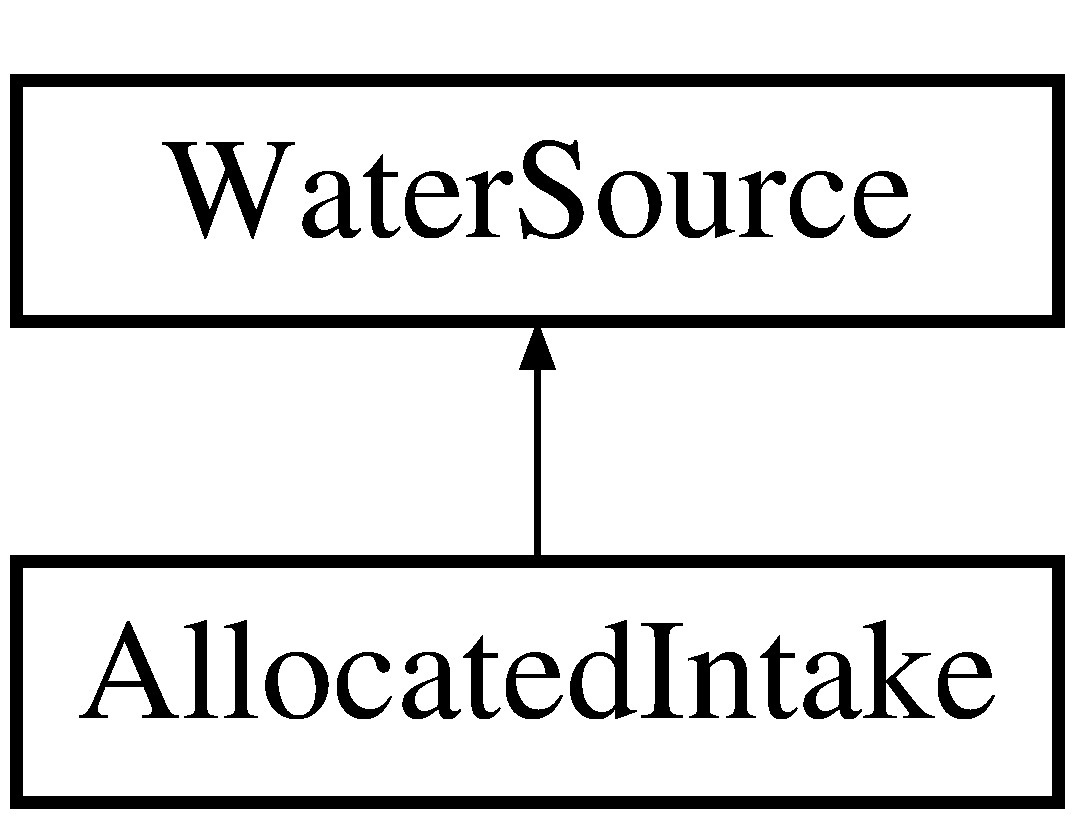
\includegraphics[height=2.000000cm]{classAllocatedIntake}
\end{center}
\end{figure}
\subsection*{Public Member Functions}
\begin{DoxyCompactItemize}
\item 
\mbox{\hyperlink{classAllocatedIntake_a06653dc837c927a68ab809234d78f505}{Allocated\+Intake}} (const char $\ast$\mbox{\hyperlink{classWaterSource_a846ea74c5b453d014f594d41fee8c765}{name}}, const int \mbox{\hyperlink{classWaterSource_a6eafe5dfefd317877d1244e8a7c6e742}{id}}, const vector$<$ \mbox{\hyperlink{classCatchment}{Catchment}} $\ast$$>$ \&\mbox{\hyperlink{classWaterSource_a8c18c34f23f8a06685c1d12f462ed830}{catchments}}, vector$<$ int $>$ connected\+\_\+sources, vector$<$ int $>$ \&partner\+\_\+utilities, const double total\+\_\+raw\+\_\+water\+\_\+capacity, vector$<$ double $>$ \&raw\+\_\+water\+\_\+capacity\+\_\+allocation\+\_\+fractions, const double \mbox{\hyperlink{classWaterSource_a2fdfd5ff7d103e71108cf2a31babaccb}{total\+\_\+treatment\+\_\+capacity}}, vector$<$ double $>$ \&treatment\+\_\+capacity\+\_\+allocation\+\_\+fractions)
\begin{DoxyCompactList}\small\item\em Constructor for creating an {\ttfamily \mbox{\hyperlink{classAllocatedIntake}{Allocated\+Intake}}} object. \end{DoxyCompactList}\item 
\mbox{\hyperlink{classAllocatedIntake_a39f2cd728b88fa1503bbe32a9165f654}{Allocated\+Intake}} (const \mbox{\hyperlink{classAllocatedIntake}{Allocated\+Intake}} \&intake)
\begin{DoxyCompactList}\small\item\em Copy constructor for creating a new {\ttfamily \mbox{\hyperlink{classAllocatedIntake}{Allocated\+Intake}}} object by copying another {\ttfamily \mbox{\hyperlink{classAllocatedIntake}{Allocated\+Intake}}} object. \end{DoxyCompactList}\item 
\mbox{\hyperlink{classAllocatedIntake}{Allocated\+Intake}} \& \mbox{\hyperlink{classAllocatedIntake_a86afa1536bf7ee7945f2c567c43ffb6b}{operator=}} (const \mbox{\hyperlink{classAllocatedIntake}{Allocated\+Intake}} \&intake)
\begin{DoxyCompactList}\small\item\em Assignment operator for copying the contents of one {\ttfamily \mbox{\hyperlink{classAllocatedIntake}{Allocated\+Intake}}} object to another. \end{DoxyCompactList}\item 
\mbox{\hyperlink{classAllocatedIntake_ada2f6552b83f4f11611bcd7bcb27fc37}{$\sim$\+Allocated\+Intake}} () override
\begin{DoxyCompactList}\small\item\em Destructor for the {\ttfamily \mbox{\hyperlink{classAllocatedIntake}{Allocated\+Intake}}} class. \end{DoxyCompactList}\item 
void \mbox{\hyperlink{classAllocatedIntake_a92c562dddb4f6434c8ad766c03b2cf5c}{apply\+Continuity}} (int week, double upstream\+\_\+source\+\_\+min\+\_\+env\+\_\+flow, double \mbox{\hyperlink{classWaterSource_aeb5a2d2d83383a70ca20f3e94635a9c7}{wastewater\+\_\+inflow}}, vector$<$ double $>$ \&demand) override
\begin{DoxyCompactList}\small\item\em Applies the continuity equation to update water availability, demand, and allocations for the current time step. \end{DoxyCompactList}\item 
void \mbox{\hyperlink{classAllocatedIntake_afc73ae38f23417cfbece54c4c3d4ccc9}{set\+Realization}} (unsigned long r, vector$<$ double $>$ \&rdm\+\_\+factors) override
\begin{DoxyCompactList}\small\item\em Sets the realization for the {\ttfamily \mbox{\hyperlink{classAllocatedIntake}{Allocated\+Intake}}} object and updates water demand and availability. \end{DoxyCompactList}\item 
double \mbox{\hyperlink{classAllocatedIntake_abbea26f2adac6c9f9e3bdcdf1aead55d}{get\+Priority\+Source\+Potential\+Volume}} (int utility\+\_\+id) const override
\begin{DoxyCompactList}\small\item\em Calculates the priority source potential volume for a given utility. \end{DoxyCompactList}\item 
vector$<$ double $>$ \mbox{\hyperlink{classAllocatedIntake_a5efc6423bff0adb8c493d3c9983915ef}{get\+Allocated\+Demands}} () const
\begin{DoxyCompactList}\small\item\em Retrieves the allocated demands for all utilities. \end{DoxyCompactList}\item 
void \mbox{\hyperlink{classAllocatedIntake_a32a52eb269d4de861cc844633eceefb0}{add\+Capacity}} (double \mbox{\hyperlink{classWaterSource_a2ec257b415b248214a8bce7fc5267723}{capacity}}, int utility\+\_\+id)
\begin{DoxyCompactList}\small\item\em Adds capacity to the {\ttfamily \mbox{\hyperlink{classAllocatedIntake}{Allocated\+Intake}}} object and updates utility allocations. \end{DoxyCompactList}\item 
void \mbox{\hyperlink{classAllocatedIntake_ae16939ed474e15b9c68edcbf61696231}{add\+Treatment\+Capacity}} (const double added\+\_\+treatment\+\_\+capacity, int utility\+\_\+id)
\begin{DoxyCompactList}\small\item\em Adds treatment capacity to the {\ttfamily \mbox{\hyperlink{classAllocatedIntake}{Allocated\+Intake}}} object and updates utility allocations. \end{DoxyCompactList}\item 
double \mbox{\hyperlink{classAllocatedIntake_a9c6161b8dd13b6ea70a9dafbb72afc91}{get\+Available\+Allocated\+Volume}} (int utility\+\_\+id) override
\begin{DoxyCompactList}\small\item\em Retrieves the available allocated volume for a specific utility. \end{DoxyCompactList}\end{DoxyCompactItemize}
\subsection*{Public Attributes}
\begin{DoxyCompactItemize}
\item 
double \mbox{\hyperlink{classAllocatedIntake_acf0824f3602cf6e9aa5c4423cb04f078}{next\+\_\+upstream\+\_\+catchment\+\_\+inflow}} = 0
\begin{DoxyCompactList}\small\item\em The inflow from the adjacent upstream catchment. \end{DoxyCompactList}\item 
vector$<$ double $>$ \mbox{\hyperlink{classAllocatedIntake_aab00f81a712fe2ecff1f69d0bb53d92a}{allocated\+\_\+demands}}
\begin{DoxyCompactList}\small\item\em The demands allocated to each utility to be fulfiled by this intake. \end{DoxyCompactList}\end{DoxyCompactItemize}
\subsection*{Additional Inherited Members}


\subsection{Detailed Description}
The {\ttfamily \mbox{\hyperlink{classAllocatedIntake}{Allocated\+Intake}}} is a subclass of the main {\ttfamily \mbox{\hyperlink{classWaterSource}{Water\+Source}}} class that represents a raw water intake from upstream catchments with allocations associated to utilities. 

Created by dgorelic on 3/2/2020. 

\subsection{Constructor \& Destructor Documentation}
\mbox{\Hypertarget{classAllocatedIntake_a06653dc837c927a68ab809234d78f505}\label{classAllocatedIntake_a06653dc837c927a68ab809234d78f505}} 
\index{Allocated\+Intake@{Allocated\+Intake}!Allocated\+Intake@{Allocated\+Intake}}
\index{Allocated\+Intake@{Allocated\+Intake}!Allocated\+Intake@{Allocated\+Intake}}
\subsubsection{\texorpdfstring{Allocated\+Intake()}{AllocatedIntake()}\hspace{0.1cm}{\footnotesize\ttfamily [1/2]}}
{\footnotesize\ttfamily Allocated\+Intake\+::\+Allocated\+Intake (\begin{DoxyParamCaption}\item[{const char $\ast$}]{name,  }\item[{const int}]{id,  }\item[{const vector$<$ \mbox{\hyperlink{classCatchment}{Catchment}} $\ast$$>$ \&}]{catchments,  }\item[{vector$<$ int $>$}]{connected\+\_\+sources,  }\item[{vector$<$ int $>$ \&}]{partner\+\_\+utilities,  }\item[{const double}]{total\+\_\+raw\+\_\+water\+\_\+capacity,  }\item[{vector$<$ double $>$ \&}]{raw\+\_\+water\+\_\+capacity\+\_\+allocation\+\_\+fractions,  }\item[{const double}]{total\+\_\+treatment\+\_\+capacity,  }\item[{vector$<$ double $>$ \&}]{treatment\+\_\+capacity\+\_\+allocation\+\_\+fractions }\end{DoxyParamCaption})}



Constructor for creating an {\ttfamily \mbox{\hyperlink{classAllocatedIntake}{Allocated\+Intake}}} object. 

This constructor initializes an {\ttfamily \mbox{\hyperlink{classAllocatedIntake}{Allocated\+Intake}}} object, which represents a intake that has allocated raw water and treatment capacities, as well as associated utilities and catchments. It initializes various properties by invoking the base class constructor ({\ttfamily \mbox{\hyperlink{classWaterSource}{Water\+Source}}}) and setting additional member variables such as {\ttfamily allocated\+\_\+demands}.


\begin{DoxyParams}{Parameters}
{\em name} & The name of the intake. \\
\hline
{\em id} & The unique identifier for the intake. \\
\hline
{\em catchments} & A vector of pointers to the catchments associated with this intake. \\
\hline
{\em connected\+\_\+sources} & A vector of I\+Ds for the connected sources of the intake. \\
\hline
{\em partner\+\_\+utilities} & A vector of I\+Ds for the partner utilities associated with this intake. \\
\hline
{\em total\+\_\+raw\+\_\+water\+\_\+capacity} & The total raw water capacity of the intake. \\
\hline
{\em raw\+\_\+water\+\_\+capacity\+\_\+allocation\+\_\+fractions} & A vector of fractions representing the allocation of raw water capacity to different utilities. \\
\hline
{\em total\+\_\+treatment\+\_\+capacity} & The total treatment capacity of the intake. \\
\hline
{\em treatment\+\_\+capacity\+\_\+allocation\+\_\+fractions} & A vector of fractions representing the allocation of treatment capacity to different utilities.\\
\hline
\end{DoxyParams}
\begin{DoxyReturn}{Returns}
A fully constructed {\ttfamily \mbox{\hyperlink{classAllocatedIntake}{Allocated\+Intake}}} object. 
\end{DoxyReturn}
\mbox{\Hypertarget{classAllocatedIntake_a39f2cd728b88fa1503bbe32a9165f654}\label{classAllocatedIntake_a39f2cd728b88fa1503bbe32a9165f654}} 
\index{Allocated\+Intake@{Allocated\+Intake}!Allocated\+Intake@{Allocated\+Intake}}
\index{Allocated\+Intake@{Allocated\+Intake}!Allocated\+Intake@{Allocated\+Intake}}
\subsubsection{\texorpdfstring{Allocated\+Intake()}{AllocatedIntake()}\hspace{0.1cm}{\footnotesize\ttfamily [2/2]}}
{\footnotesize\ttfamily Allocated\+Intake\+::\+Allocated\+Intake (\begin{DoxyParamCaption}\item[{const \mbox{\hyperlink{classAllocatedIntake}{Allocated\+Intake}} \&}]{intake }\end{DoxyParamCaption})}



Copy constructor for creating a new {\ttfamily \mbox{\hyperlink{classAllocatedIntake}{Allocated\+Intake}}} object by copying another {\ttfamily \mbox{\hyperlink{classAllocatedIntake}{Allocated\+Intake}}} object. 

This constructor initializes a new {\ttfamily \mbox{\hyperlink{classAllocatedIntake}{Allocated\+Intake}}} object by copying the values from an existing {\ttfamily \mbox{\hyperlink{classAllocatedIntake}{Allocated\+Intake}}} object. It delegates the initialization of the base class ({\ttfamily \mbox{\hyperlink{classWaterSource}{Water\+Source}}}) to the base class copy constructor and copies the {\ttfamily allocated\+\_\+demands} vector from the intake object.


\begin{DoxyParams}{Parameters}
{\em intake} & The {\ttfamily \mbox{\hyperlink{classAllocatedIntake}{Allocated\+Intake}}} object to copy from.\\
\hline
\end{DoxyParams}
\begin{DoxyReturn}{Returns}
A new {\ttfamily \mbox{\hyperlink{classAllocatedIntake}{Allocated\+Intake}}} object that is a copy of the provided {\ttfamily intake} object. 
\end{DoxyReturn}
\mbox{\Hypertarget{classAllocatedIntake_ada2f6552b83f4f11611bcd7bcb27fc37}\label{classAllocatedIntake_ada2f6552b83f4f11611bcd7bcb27fc37}} 
\index{Allocated\+Intake@{Allocated\+Intake}!````~Allocated\+Intake@{$\sim$\+Allocated\+Intake}}
\index{````~Allocated\+Intake@{$\sim$\+Allocated\+Intake}!Allocated\+Intake@{Allocated\+Intake}}
\subsubsection{\texorpdfstring{$\sim$\+Allocated\+Intake()}{~AllocatedIntake()}}
{\footnotesize\ttfamily Allocated\+Intake\+::$\sim$\+Allocated\+Intake (\begin{DoxyParamCaption}{ }\end{DoxyParamCaption})\hspace{0.3cm}{\ttfamily [override]}}



Destructor for the {\ttfamily \mbox{\hyperlink{classAllocatedIntake}{Allocated\+Intake}}} class. 

This destructor is responsible for cleaning up the resources used by the {\ttfamily \mbox{\hyperlink{classAllocatedIntake}{Allocated\+Intake}}} object. It clears the {\ttfamily catchments} vector to free any associated memory when the object is destroyed.

This destructor overrides the base class destructor ({\ttfamily \mbox{\hyperlink{classWaterSource}{Water\+Source}}}) to ensure proper cleanup.

\begin{DoxyReturn}{Returns}
void 
\end{DoxyReturn}


\subsection{Member Function Documentation}
\mbox{\Hypertarget{classAllocatedIntake_a32a52eb269d4de861cc844633eceefb0}\label{classAllocatedIntake_a32a52eb269d4de861cc844633eceefb0}} 
\index{Allocated\+Intake@{Allocated\+Intake}!add\+Capacity@{add\+Capacity}}
\index{add\+Capacity@{add\+Capacity}!Allocated\+Intake@{Allocated\+Intake}}
\subsubsection{\texorpdfstring{add\+Capacity()}{addCapacity()}}
{\footnotesize\ttfamily void Allocated\+Intake\+::add\+Capacity (\begin{DoxyParamCaption}\item[{double}]{capacity,  }\item[{int}]{utility\+\_\+id }\end{DoxyParamCaption})\hspace{0.3cm}{\ttfamily [virtual]}}



Adds capacity to the {\ttfamily \mbox{\hyperlink{classAllocatedIntake}{Allocated\+Intake}}} object and updates utility allocations. 

This function adds the specified capacity to both the total capacity of the {\ttfamily \mbox{\hyperlink{classAllocatedIntake}{Allocated\+Intake}}} object and the allocated capacity for a specific utility. It also ensures that the allocation fractions for all utilities are updated to reflect the new capacity.


\begin{DoxyParams}{Parameters}
{\em capacity} & The amount of capacity to add to the {\ttfamily \mbox{\hyperlink{classAllocatedIntake}{Allocated\+Intake}}}. \\
\hline
{\em utility\+\_\+id} & The ID of the utility for which the capacity is being added.\\
\hline
\end{DoxyParams}
\begin{DoxyReturn}{Returns}
void 
\end{DoxyReturn}


Reimplemented from \mbox{\hyperlink{classWaterSource_ab869abb3d3dde1875e933482bedc3ae3}{Water\+Source}}.

\mbox{\Hypertarget{classAllocatedIntake_ae16939ed474e15b9c68edcbf61696231}\label{classAllocatedIntake_ae16939ed474e15b9c68edcbf61696231}} 
\index{Allocated\+Intake@{Allocated\+Intake}!add\+Treatment\+Capacity@{add\+Treatment\+Capacity}}
\index{add\+Treatment\+Capacity@{add\+Treatment\+Capacity}!Allocated\+Intake@{Allocated\+Intake}}
\subsubsection{\texorpdfstring{add\+Treatment\+Capacity()}{addTreatmentCapacity()}}
{\footnotesize\ttfamily void Allocated\+Intake\+::add\+Treatment\+Capacity (\begin{DoxyParamCaption}\item[{const double}]{added\+\_\+treatment\+\_\+capacity,  }\item[{int}]{utility\+\_\+id }\end{DoxyParamCaption})\hspace{0.3cm}{\ttfamily [virtual]}}



Adds treatment capacity to the {\ttfamily \mbox{\hyperlink{classAllocatedIntake}{Allocated\+Intake}}} object and updates utility allocations. 

This function adds the specified treatment capacity to both the total treatment capacity of the {\ttfamily \mbox{\hyperlink{classAllocatedIntake}{Allocated\+Intake}}} object and the allocated treatment capacity for a specific utility. It also ensures that the allocation fractions for all utilities are updated to reflect the new treatment capacity.


\begin{DoxyParams}{Parameters}
{\em added\+\_\+treatment\+\_\+capacity} & The amount of treatment capacity to add to the {\ttfamily \mbox{\hyperlink{classAllocatedIntake}{Allocated\+Intake}}}. \\
\hline
{\em utility\+\_\+id} & The ID of the utility for which the treatment capacity is being added.\\
\hline
\end{DoxyParams}
\begin{DoxyReturn}{Returns}
void 
\end{DoxyReturn}


Reimplemented from \mbox{\hyperlink{classWaterSource_ac2bc1a09fce3a3201d62a73052b27b0b}{Water\+Source}}.

\mbox{\Hypertarget{classAllocatedIntake_a92c562dddb4f6434c8ad766c03b2cf5c}\label{classAllocatedIntake_a92c562dddb4f6434c8ad766c03b2cf5c}} 
\index{Allocated\+Intake@{Allocated\+Intake}!apply\+Continuity@{apply\+Continuity}}
\index{apply\+Continuity@{apply\+Continuity}!Allocated\+Intake@{Allocated\+Intake}}
\subsubsection{\texorpdfstring{apply\+Continuity()}{applyContinuity()}}
{\footnotesize\ttfamily void Allocated\+Intake\+::apply\+Continuity (\begin{DoxyParamCaption}\item[{int}]{week,  }\item[{double}]{upstream\+\_\+source\+\_\+min\+\_\+env\+\_\+flow,  }\item[{double}]{wastewater\+\_\+inflow,  }\item[{vector$<$ double $>$ \&}]{demand }\end{DoxyParamCaption})\hspace{0.3cm}{\ttfamily [override]}, {\ttfamily [virtual]}}



Applies the continuity equation to update water availability, demand, and allocations for the current time step. 

This function updates various properties related to water inflow, outflow, and demand based on the continuity equation. It computes the total upstream inflows, allocates available volumes to utilities based on their allocations, and updates the outflows and demands for the current week.

This function overrides the base class method {\ttfamily apply\+Continuity} to provide specific implementation for {\ttfamily \mbox{\hyperlink{classAllocatedIntake}{Allocated\+Intake}}}.


\begin{DoxyParams}{Parameters}
{\em week} & The current week for which the continuity equation is being applied. \\
\hline
{\em upstream\+\_\+source\+\_\+min\+\_\+env\+\_\+flow} & The minimum environmental flow from upstream sources. \\
\hline
{\em wastewater\+\_\+inflow} & The inflow of wastewater. \\
\hline
{\em demand} & A fraction of supply allocated to demands from each utility.\\
\hline
\end{DoxyParams}
\begin{DoxyReturn}{Returns}
void 
\end{DoxyReturn}


Implements \mbox{\hyperlink{classWaterSource_ac070445379fe706f65b977dade4f3fbc}{Water\+Source}}.

\mbox{\Hypertarget{classAllocatedIntake_a5efc6423bff0adb8c493d3c9983915ef}\label{classAllocatedIntake_a5efc6423bff0adb8c493d3c9983915ef}} 
\index{Allocated\+Intake@{Allocated\+Intake}!get\+Allocated\+Demands@{get\+Allocated\+Demands}}
\index{get\+Allocated\+Demands@{get\+Allocated\+Demands}!Allocated\+Intake@{Allocated\+Intake}}
\subsubsection{\texorpdfstring{get\+Allocated\+Demands()}{getAllocatedDemands()}}
{\footnotesize\ttfamily vector$<$double$>$ Allocated\+Intake\+::get\+Allocated\+Demands (\begin{DoxyParamCaption}{ }\end{DoxyParamCaption}) const}



Retrieves the allocated demands for all utilities. 

This function returns a vector containing the allocated demands for all utilities associated with the {\ttfamily \mbox{\hyperlink{classAllocatedIntake}{Allocated\+Intake}}} object. The demands are represented by the {\ttfamily allocated\+\_\+demands} vector, which is updated based on the current inflows and allocations.

\begin{DoxyReturn}{Returns}
A vector of {\ttfamily double} representing the allocated demands for each utility. 
\end{DoxyReturn}
\mbox{\Hypertarget{classAllocatedIntake_a9c6161b8dd13b6ea70a9dafbb72afc91}\label{classAllocatedIntake_a9c6161b8dd13b6ea70a9dafbb72afc91}} 
\index{Allocated\+Intake@{Allocated\+Intake}!get\+Available\+Allocated\+Volume@{get\+Available\+Allocated\+Volume}}
\index{get\+Available\+Allocated\+Volume@{get\+Available\+Allocated\+Volume}!Allocated\+Intake@{Allocated\+Intake}}
\subsubsection{\texorpdfstring{get\+Available\+Allocated\+Volume()}{getAvailableAllocatedVolume()}}
{\footnotesize\ttfamily double Allocated\+Intake\+::get\+Available\+Allocated\+Volume (\begin{DoxyParamCaption}\item[{int}]{utility\+\_\+id }\end{DoxyParamCaption})\hspace{0.3cm}{\ttfamily [override]}, {\ttfamily [virtual]}}



Retrieves the available allocated volume for a specific utility. 

This function returns the available allocated volume for a given utility. The available volume is determined based on the current allocation and environmental conditions. This function overrides the base class method {\ttfamily get\+Available\+Allocated\+Volume} to provide specific implementation for {\ttfamily \mbox{\hyperlink{classAllocatedIntake}{Allocated\+Intake}}}.


\begin{DoxyParams}{Parameters}
{\em utility\+\_\+id} & The ID of the utility for which the available allocated volume is being retrieved.\\
\hline
\end{DoxyParams}
\begin{DoxyReturn}{Returns}
The available allocated volume for the specified utility. 
\end{DoxyReturn}


Reimplemented from \mbox{\hyperlink{classWaterSource_ad4667296dc6b6dabc36b871529ca2749}{Water\+Source}}.

\mbox{\Hypertarget{classAllocatedIntake_abbea26f2adac6c9f9e3bdcdf1aead55d}\label{classAllocatedIntake_abbea26f2adac6c9f9e3bdcdf1aead55d}} 
\index{Allocated\+Intake@{Allocated\+Intake}!get\+Priority\+Source\+Potential\+Volume@{get\+Priority\+Source\+Potential\+Volume}}
\index{get\+Priority\+Source\+Potential\+Volume@{get\+Priority\+Source\+Potential\+Volume}!Allocated\+Intake@{Allocated\+Intake}}
\subsubsection{\texorpdfstring{get\+Priority\+Source\+Potential\+Volume()}{getPrioritySourcePotentialVolume()}}
{\footnotesize\ttfamily double Allocated\+Intake\+::get\+Priority\+Source\+Potential\+Volume (\begin{DoxyParamCaption}\item[{int}]{utility\+\_\+id }\end{DoxyParamCaption}) const\hspace{0.3cm}{\ttfamily [override]}, {\ttfamily [virtual]}}



Calculates the priority source potential volume for a given utility. 

This function calculates the potential volume of water available to a utility based on its allocated treatment capacity, current demand, environmental requirements, and upstream catchment inflow. The result is the maximum available volume that can be allocated to the utility, considering the constraints set by treatment capacities and environmental flows.

This function overrides the base class method {\ttfamily get\+Priority\+Source\+Potential\+Volume} to provide specific implementation for {\ttfamily \mbox{\hyperlink{classAllocatedIntake}{Allocated\+Intake}}}.


\begin{DoxyParams}{Parameters}
{\em utility\+\_\+id} & The ID of the utility for which the priority source potential volume is being calculated.\\
\hline
\end{DoxyParams}
\begin{DoxyReturn}{Returns}
The calculated priority source potential volume for the specified utility. 
\end{DoxyReturn}


Reimplemented from \mbox{\hyperlink{classWaterSource_a00a432eba75eaae7195338a8514ac853}{Water\+Source}}.

\mbox{\Hypertarget{classAllocatedIntake_a86afa1536bf7ee7945f2c567c43ffb6b}\label{classAllocatedIntake_a86afa1536bf7ee7945f2c567c43ffb6b}} 
\index{Allocated\+Intake@{Allocated\+Intake}!operator=@{operator=}}
\index{operator=@{operator=}!Allocated\+Intake@{Allocated\+Intake}}
\subsubsection{\texorpdfstring{operator=()}{operator=()}}
{\footnotesize\ttfamily \mbox{\hyperlink{classAllocatedIntake}{Allocated\+Intake}}\& Allocated\+Intake\+::operator= (\begin{DoxyParamCaption}\item[{const \mbox{\hyperlink{classAllocatedIntake}{Allocated\+Intake}} \&}]{intake }\end{DoxyParamCaption})}



Assignment operator for copying the contents of one {\ttfamily \mbox{\hyperlink{classAllocatedIntake}{Allocated\+Intake}}} object to another. 

This operator allows for the assignment of one {\ttfamily \mbox{\hyperlink{classAllocatedIntake}{Allocated\+Intake}}} object to another, copying the values of the base class ({\ttfamily \mbox{\hyperlink{classWaterSource}{Water\+Source}}}) and the {\ttfamily allocated\+\_\+demands} vector from the source object to the target object.


\begin{DoxyParams}{Parameters}
{\em intake} & The {\ttfamily \mbox{\hyperlink{classAllocatedIntake}{Allocated\+Intake}}} object to assign from.\\
\hline
\end{DoxyParams}
\begin{DoxyReturn}{Returns}
A reference to the target {\ttfamily \mbox{\hyperlink{classAllocatedIntake}{Allocated\+Intake}}} object ({\ttfamily $\ast$this}). 
\end{DoxyReturn}
\mbox{\Hypertarget{classAllocatedIntake_afc73ae38f23417cfbece54c4c3d4ccc9}\label{classAllocatedIntake_afc73ae38f23417cfbece54c4c3d4ccc9}} 
\index{Allocated\+Intake@{Allocated\+Intake}!set\+Realization@{set\+Realization}}
\index{set\+Realization@{set\+Realization}!Allocated\+Intake@{Allocated\+Intake}}
\subsubsection{\texorpdfstring{set\+Realization()}{setRealization()}}
{\footnotesize\ttfamily void Allocated\+Intake\+::set\+Realization (\begin{DoxyParamCaption}\item[{unsigned long}]{r,  }\item[{vector$<$ double $>$ \&}]{rdm\+\_\+factors }\end{DoxyParamCaption})\hspace{0.3cm}{\ttfamily [override]}, {\ttfamily [virtual]}}



Sets the realization for the {\ttfamily \mbox{\hyperlink{classAllocatedIntake}{Allocated\+Intake}}} object and updates water demand and availability. 

This function sets the realization for the {\ttfamily \mbox{\hyperlink{classAllocatedIntake}{Allocated\+Intake}}} object by calling the base class\textquotesingle{}s {\ttfamily set\+Realization} method. It then updates the total demand and available volume based on the current upstream catchment inflow and the minimum environmental outflow.

This function overrides the base class method {\ttfamily set\+Realization} to provide specific implementation for {\ttfamily \mbox{\hyperlink{classAllocatedIntake}{Allocated\+Intake}}}.


\begin{DoxyParams}{Parameters}
{\em r} & The realization index (e.\+g., representing a specific scenario or time step). \\
\hline
{\em rdm\+\_\+factors} & A vector of random distribution factors used in the realization process.\\
\hline
\end{DoxyParams}
\begin{DoxyReturn}{Returns}
void 
\end{DoxyReturn}


Reimplemented from \mbox{\hyperlink{classWaterSource_a634904c510b16de6d7c057fed6d6e625}{Water\+Source}}.



\subsection{Member Data Documentation}
\mbox{\Hypertarget{classAllocatedIntake_aab00f81a712fe2ecff1f69d0bb53d92a}\label{classAllocatedIntake_aab00f81a712fe2ecff1f69d0bb53d92a}} 
\index{Allocated\+Intake@{Allocated\+Intake}!allocated\+\_\+demands@{allocated\+\_\+demands}}
\index{allocated\+\_\+demands@{allocated\+\_\+demands}!Allocated\+Intake@{Allocated\+Intake}}
\subsubsection{\texorpdfstring{allocated\+\_\+demands}{allocated\_demands}}
{\footnotesize\ttfamily vector$<$double$>$ Allocated\+Intake\+::allocated\+\_\+demands}



The demands allocated to each utility to be fulfiled by this intake. 

\mbox{\Hypertarget{classAllocatedIntake_acf0824f3602cf6e9aa5c4423cb04f078}\label{classAllocatedIntake_acf0824f3602cf6e9aa5c4423cb04f078}} 
\index{Allocated\+Intake@{Allocated\+Intake}!next\+\_\+upstream\+\_\+catchment\+\_\+inflow@{next\+\_\+upstream\+\_\+catchment\+\_\+inflow}}
\index{next\+\_\+upstream\+\_\+catchment\+\_\+inflow@{next\+\_\+upstream\+\_\+catchment\+\_\+inflow}!Allocated\+Intake@{Allocated\+Intake}}
\subsubsection{\texorpdfstring{next\+\_\+upstream\+\_\+catchment\+\_\+inflow}{next\_upstream\_catchment\_inflow}}
{\footnotesize\ttfamily double Allocated\+Intake\+::next\+\_\+upstream\+\_\+catchment\+\_\+inflow = 0}



The inflow from the adjacent upstream catchment. 



The documentation for this class was generated from the following file\+:\begin{DoxyCompactItemize}
\item 
src/\+System\+Components/\+Water\+Sources/\mbox{\hyperlink{AllocatedIntake_8h}{Allocated\+Intake.\+h}}\end{DoxyCompactItemize}

\hypertarget{classAllocatedIntakeExpansion}{}\section{Allocated\+Intake\+Expansion Class Reference}
\label{classAllocatedIntakeExpansion}\index{Allocated\+Intake\+Expansion@{Allocated\+Intake\+Expansion}}


The {\ttfamily \mbox{\hyperlink{classAllocatedIntakeExpansion}{Allocated\+Intake\+Expansion}}} is a subclass of the main {\ttfamily \mbox{\hyperlink{classWaterSource}{Water\+Source}}} class that represents a raw water intake from upstream catchments with allocations associated to utilities.  




{\ttfamily \#include $<$Allocated\+Intake\+Expansion.\+h$>$}

Inheritance diagram for Allocated\+Intake\+Expansion\+:\begin{figure}[H]
\begin{center}
\leavevmode
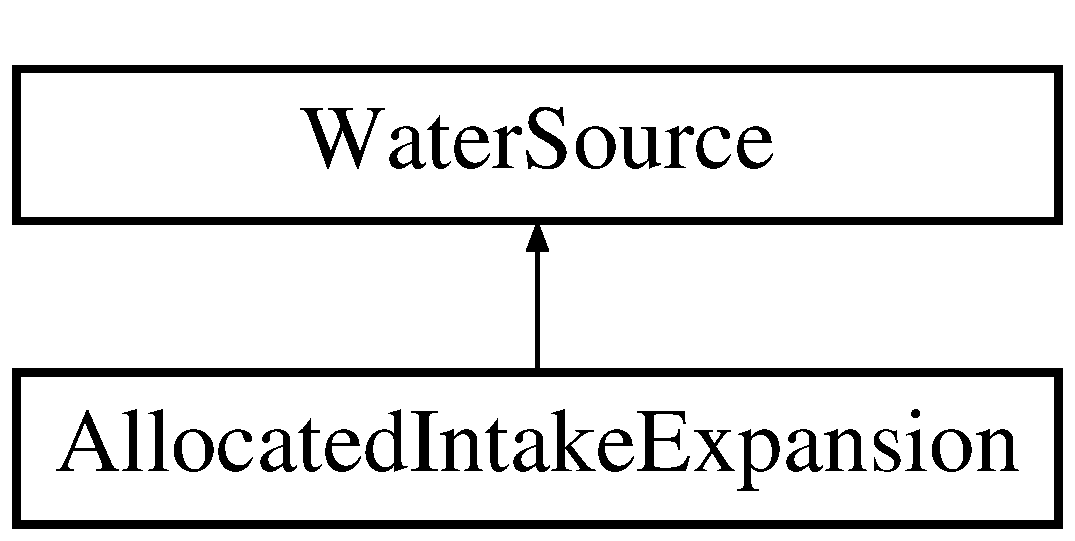
\includegraphics[height=2.000000cm]{classAllocatedIntakeExpansion}
\end{center}
\end{figure}
\subsection*{Public Member Functions}
\begin{DoxyCompactItemize}
\item 
\mbox{\hyperlink{classAllocatedIntakeExpansion_a4ed3330e33441d67d3b0c8bbb243d6c2}{Allocated\+Intake\+Expansion}} (const char $\ast$\mbox{\hyperlink{classWaterSource_a846ea74c5b453d014f594d41fee8c765}{name}}, const int \mbox{\hyperlink{classWaterSource_a6eafe5dfefd317877d1244e8a7c6e742}{id}}, const unsigned int \mbox{\hyperlink{classAllocatedIntakeExpansion_a725ce7276ef9158da9fa7e2b1e217b14}{parent\+\_\+intake\+\_\+\+ID}}, const double total\+\_\+supply\+\_\+capacity\+\_\+added, double total\+\_\+treatment\+\_\+capacity\+\_\+added, vector$<$ int $>$ \&partner\+\_\+utility\+\_\+ids, vector$<$ double $>$ \&supply\+\_\+capacity\+\_\+allocations\+\_\+added, vector$<$ double $>$ \&treatment\+\_\+capacity\+\_\+allocations\+\_\+added, const vector$<$ double $>$ \&construction\+\_\+time\+\_\+range, vector$<$ int $>$ connected\+\_\+sources, double permitting\+\_\+period, vector$<$ \mbox{\hyperlink{classBond}{Bond}} $\ast$$>$ \&\mbox{\hyperlink{classWaterSource_a413b094e11bdce62f4d82e5bb9e4706e}{bonds}})
\begin{DoxyCompactList}\small\item\em Constructor for creating an {\ttfamily \mbox{\hyperlink{classAllocatedIntakeExpansion}{Allocated\+Intake\+Expansion}}} object. \end{DoxyCompactList}\item 
\mbox{\hyperlink{classAllocatedIntakeExpansion_a5789688f1a053b4f3201470aedece0cc}{Allocated\+Intake\+Expansion}} (const \mbox{\hyperlink{classAllocatedIntakeExpansion}{Allocated\+Intake\+Expansion}} \&intake\+\_\+expansion)
\begin{DoxyCompactList}\small\item\em Copy constructor for creating a copy of an {\ttfamily \mbox{\hyperlink{classAllocatedIntakeExpansion}{Allocated\+Intake\+Expansion}}} object. \end{DoxyCompactList}\item 
\mbox{\hyperlink{classAllocatedIntakeExpansion}{Allocated\+Intake\+Expansion}} \& \mbox{\hyperlink{classAllocatedIntakeExpansion_a3c695346b66343278a51c3df50866acb}{operator=}} (const \mbox{\hyperlink{classAllocatedIntakeExpansion}{Allocated\+Intake\+Expansion}} \&intake\+\_\+expansion)
\begin{DoxyCompactList}\small\item\em Assignment operator for copying an {\ttfamily \mbox{\hyperlink{classAllocatedIntakeExpansion}{Allocated\+Intake\+Expansion}}} object. \end{DoxyCompactList}\item 
void \mbox{\hyperlink{classAllocatedIntakeExpansion_a67185ec779549c32b289666663232bc4}{apply\+Continuity}} (int week, double \mbox{\hyperlink{classWaterSource_a7a69b2e9b6030f1035e6cf44d2918ee5}{upstream\+\_\+source\+\_\+inflow}}, double wastewater\+\_\+discharge, vector$<$ double $>$ \&demand\+\_\+outflow) override
\begin{DoxyCompactList}\small\item\em Applies continuity for the intake expansion, updating the available flow and demand outflows. \end{DoxyCompactList}\item 
double \mbox{\hyperlink{classAllocatedIntakeExpansion_a6cd2dabeb1dc1e0417082c032620ce51}{get\+Allocated\+Capacity}} (int utility\+\_\+id) override
\begin{DoxyCompactList}\small\item\em Retrieves the allocated supply capacity for a specific utility. \end{DoxyCompactList}\item 
double \mbox{\hyperlink{classAllocatedIntakeExpansion_a20fb863c5e0bce30c10d1791b037a57a}{get\+Allocated\+Treatment\+Capacity}} (int utility\+\_\+id) const override
\begin{DoxyCompactList}\small\item\em Retrieves the allocated treatment capacity for a specific utility. \end{DoxyCompactList}\item 
\mbox{\hyperlink{classBond}{Bond}} \& \mbox{\hyperlink{classAllocatedIntakeExpansion_a3091edd0793cf2bd4e01fc178ae72ffb}{get\+Bond}} (int utility\+\_\+id) override
\begin{DoxyCompactList}\small\item\em Retrieves the bond associated with a specific utility. \end{DoxyCompactList}\end{DoxyCompactItemize}
\subsection*{Public Attributes}
\begin{DoxyCompactItemize}
\item 
const unsigned int \mbox{\hyperlink{classAllocatedIntakeExpansion_a725ce7276ef9158da9fa7e2b1e217b14}{parent\+\_\+intake\+\_\+\+ID}}
\begin{DoxyCompactList}\small\item\em The water source ID of the parent intake object. \end{DoxyCompactList}\item 
const vector$<$ double $>$ \mbox{\hyperlink{classAllocatedIntakeExpansion_ad788b8373f3e8c9eb2a910c370e91f7c}{supply\+\_\+capacity\+\_\+added}}
\begin{DoxyCompactList}\small\item\em A vector of the supply capacity added to the intake for each utility with allocation to this intake. \end{DoxyCompactList}\item 
const vector$<$ double $>$ \mbox{\hyperlink{classAllocatedIntakeExpansion_a22f6d50982db1cf862e81672612abdb9}{treatment\+\_\+capacity\+\_\+added}}
\begin{DoxyCompactList}\small\item\em A vector of the treatment capacity added to the intake for each utility with allocation to this intake. \end{DoxyCompactList}\end{DoxyCompactItemize}
\subsection*{Additional Inherited Members}


\subsection{Detailed Description}
The {\ttfamily \mbox{\hyperlink{classAllocatedIntakeExpansion}{Allocated\+Intake\+Expansion}}} is a subclass of the main {\ttfamily \mbox{\hyperlink{classWaterSource}{Water\+Source}}} class that represents a raw water intake from upstream catchments with allocations associated to utilities. 

Created by dgorelic on 3/2/2020. 

\subsection{Constructor \& Destructor Documentation}
\mbox{\Hypertarget{classAllocatedIntakeExpansion_a4ed3330e33441d67d3b0c8bbb243d6c2}\label{classAllocatedIntakeExpansion_a4ed3330e33441d67d3b0c8bbb243d6c2}} 
\index{Allocated\+Intake\+Expansion@{Allocated\+Intake\+Expansion}!Allocated\+Intake\+Expansion@{Allocated\+Intake\+Expansion}}
\index{Allocated\+Intake\+Expansion@{Allocated\+Intake\+Expansion}!Allocated\+Intake\+Expansion@{Allocated\+Intake\+Expansion}}
\subsubsection{\texorpdfstring{Allocated\+Intake\+Expansion()}{AllocatedIntakeExpansion()}\hspace{0.1cm}{\footnotesize\ttfamily [1/2]}}
{\footnotesize\ttfamily Allocated\+Intake\+Expansion\+::\+Allocated\+Intake\+Expansion (\begin{DoxyParamCaption}\item[{const char $\ast$}]{name,  }\item[{const int}]{id,  }\item[{const unsigned int}]{parent\+\_\+intake\+\_\+\+ID,  }\item[{const double}]{total\+\_\+supply\+\_\+capacity\+\_\+added,  }\item[{double}]{total\+\_\+treatment\+\_\+capacity\+\_\+added,  }\item[{vector$<$ int $>$ \&}]{partner\+\_\+utility\+\_\+ids,  }\item[{vector$<$ double $>$ \&}]{supply\+\_\+capacity\+\_\+allocations\+\_\+added,  }\item[{vector$<$ double $>$ \&}]{treatment\+\_\+capacity\+\_\+allocations\+\_\+added,  }\item[{const vector$<$ double $>$ \&}]{construction\+\_\+time\+\_\+range,  }\item[{vector$<$ int $>$}]{connected\+\_\+sources,  }\item[{double}]{permitting\+\_\+period,  }\item[{vector$<$ \mbox{\hyperlink{classBond}{Bond}} $\ast$$>$ \&}]{bonds }\end{DoxyParamCaption})}



Constructor for creating an {\ttfamily \mbox{\hyperlink{classAllocatedIntakeExpansion}{Allocated\+Intake\+Expansion}}} object. 

This constructor initializes an {\ttfamily \mbox{\hyperlink{classAllocatedIntakeExpansion}{Allocated\+Intake\+Expansion}}} object by calling the base class\textquotesingle{}s {\ttfamily \mbox{\hyperlink{classWaterSource}{Water\+Source}}} constructor and setting additional specific attributes for the expansion, such as supply and treatment capacities, construction time range, and partner utilities. It also stores the parent intake ID and updates the relevant capacities for the expansion.


\begin{DoxyParams}{Parameters}
{\em name} & The name of the intake expansion. \\
\hline
{\em id} & The unique identifier for the intake expansion. \\
\hline
{\em parent\+\_\+intake\+\_\+\+ID} & The ID of the parent intake to which this expansion is associated. \\
\hline
{\em total\+\_\+supply\+\_\+capacity\+\_\+added} & The total additional supply capacity for the expansion. \\
\hline
{\em total\+\_\+treatment\+\_\+capacity\+\_\+added} & The total additional treatment capacity for the expansion. \\
\hline
{\em partner\+\_\+utility\+\_\+ids} & A vector of I\+Ds representing the utilities involved with this expansion. \\
\hline
{\em supply\+\_\+capacity\+\_\+allocations\+\_\+added} & A vector of allocation fractions for the added supply capacity. \\
\hline
{\em treatment\+\_\+capacity\+\_\+allocations\+\_\+added} & A vector of allocation fractions for the added treatment capacity. \\
\hline
{\em construction\+\_\+time\+\_\+range} & A vector containing the range of possible construction times for the expansion. \\
\hline
{\em connected\+\_\+sources} & A vector of water source I\+Ds connected to the intake expansion. \\
\hline
{\em permitting\+\_\+period} & The permitting period for the expansion. \\
\hline
{\em bonds} & A vector of {\ttfamily \mbox{\hyperlink{classBond}{Bond}}} objects associated with the intake expansion.\\
\hline
\end{DoxyParams}
\begin{DoxyReturn}{Returns}
An {\ttfamily \mbox{\hyperlink{classAllocatedIntakeExpansion}{Allocated\+Intake\+Expansion}}} object initialized with the provided parameters. 
\end{DoxyReturn}
\mbox{\Hypertarget{classAllocatedIntakeExpansion_a5789688f1a053b4f3201470aedece0cc}\label{classAllocatedIntakeExpansion_a5789688f1a053b4f3201470aedece0cc}} 
\index{Allocated\+Intake\+Expansion@{Allocated\+Intake\+Expansion}!Allocated\+Intake\+Expansion@{Allocated\+Intake\+Expansion}}
\index{Allocated\+Intake\+Expansion@{Allocated\+Intake\+Expansion}!Allocated\+Intake\+Expansion@{Allocated\+Intake\+Expansion}}
\subsubsection{\texorpdfstring{Allocated\+Intake\+Expansion()}{AllocatedIntakeExpansion()}\hspace{0.1cm}{\footnotesize\ttfamily [2/2]}}
{\footnotesize\ttfamily Allocated\+Intake\+Expansion\+::\+Allocated\+Intake\+Expansion (\begin{DoxyParamCaption}\item[{const \mbox{\hyperlink{classAllocatedIntakeExpansion}{Allocated\+Intake\+Expansion}} \&}]{intake\+\_\+expansion }\end{DoxyParamCaption})}



Copy constructor for creating a copy of an {\ttfamily \mbox{\hyperlink{classAllocatedIntakeExpansion}{Allocated\+Intake\+Expansion}}} object. 

This constructor creates a new {\ttfamily \mbox{\hyperlink{classAllocatedIntakeExpansion}{Allocated\+Intake\+Expansion}}} object by copying the values from another {\ttfamily \mbox{\hyperlink{classAllocatedIntakeExpansion}{Allocated\+Intake\+Expansion}}} object. It calls the base class\textquotesingle{}s copy constructor to copy common attributes and also copies the specific attributes related to the intake expansion, such as the {\ttfamily parent\+\_\+intake\+\_\+\+ID}, {\ttfamily supply\+\_\+capacity\+\_\+added}, and {\ttfamily treatment\+\_\+capacity\+\_\+added}.


\begin{DoxyParams}{Parameters}
{\em intake\+\_\+expansion} & The {\ttfamily \mbox{\hyperlink{classAllocatedIntakeExpansion}{Allocated\+Intake\+Expansion}}} object to copy.\\
\hline
\end{DoxyParams}
\begin{DoxyReturn}{Returns}
A new {\ttfamily \mbox{\hyperlink{classAllocatedIntakeExpansion}{Allocated\+Intake\+Expansion}}} object that is a copy of the provided {\ttfamily intake\+\_\+expansion}. 
\end{DoxyReturn}


\subsection{Member Function Documentation}
\mbox{\Hypertarget{classAllocatedIntakeExpansion_a67185ec779549c32b289666663232bc4}\label{classAllocatedIntakeExpansion_a67185ec779549c32b289666663232bc4}} 
\index{Allocated\+Intake\+Expansion@{Allocated\+Intake\+Expansion}!apply\+Continuity@{apply\+Continuity}}
\index{apply\+Continuity@{apply\+Continuity}!Allocated\+Intake\+Expansion@{Allocated\+Intake\+Expansion}}
\subsubsection{\texorpdfstring{apply\+Continuity()}{applyContinuity()}}
{\footnotesize\ttfamily void Allocated\+Intake\+Expansion\+::apply\+Continuity (\begin{DoxyParamCaption}\item[{int}]{week,  }\item[{double}]{upstream\+\_\+source\+\_\+inflow,  }\item[{double}]{wastewater\+\_\+discharge,  }\item[{vector$<$ double $>$ \&}]{demand\+\_\+outflow }\end{DoxyParamCaption})\hspace{0.3cm}{\ttfamily [override]}, {\ttfamily [virtual]}}



Applies continuity for the intake expansion, updating the available flow and demand outflows. 

This function computes the continuity for the intake expansion based on the current week’s inflows, wastewater discharge, and the demand outflows. It updates the relevant internal variables to ensure the system’s water balance is maintained. This function does not have a specific implementation in this subclass, inheriting its behavior from the base class.


\begin{DoxyParams}{Parameters}
{\em week} & The week for which the continuity is being applied. \\
\hline
{\em upstream\+\_\+source\+\_\+inflow} & The inflow into the intake from the upstream source. \\
\hline
{\em wastewater\+\_\+discharge} & The volume of wasterwater discharged by the intake. \\
\hline
{\em demand\+\_\+outflow} & A vector containing the demand outflows for each associated utility.\\
\hline
\end{DoxyParams}
\begin{DoxyReturn}{Returns}
None 
\end{DoxyReturn}


Implements \mbox{\hyperlink{classWaterSource_ac070445379fe706f65b977dade4f3fbc}{Water\+Source}}.

\mbox{\Hypertarget{classAllocatedIntakeExpansion_a6cd2dabeb1dc1e0417082c032620ce51}\label{classAllocatedIntakeExpansion_a6cd2dabeb1dc1e0417082c032620ce51}} 
\index{Allocated\+Intake\+Expansion@{Allocated\+Intake\+Expansion}!get\+Allocated\+Capacity@{get\+Allocated\+Capacity}}
\index{get\+Allocated\+Capacity@{get\+Allocated\+Capacity}!Allocated\+Intake\+Expansion@{Allocated\+Intake\+Expansion}}
\subsubsection{\texorpdfstring{get\+Allocated\+Capacity()}{getAllocatedCapacity()}}
{\footnotesize\ttfamily double Allocated\+Intake\+Expansion\+::get\+Allocated\+Capacity (\begin{DoxyParamCaption}\item[{int}]{utility\+\_\+id }\end{DoxyParamCaption})\hspace{0.3cm}{\ttfamily [override]}, {\ttfamily [virtual]}}



Retrieves the allocated supply capacity for a specific utility. 

This function locates the utility within the allocation list and returns the allocated supply capacity for the given utility. This function overrides the base class implementation to handle the specific allocation structure of the intake expansion.


\begin{DoxyParams}{Parameters}
{\em utility\+\_\+id} & The ID of the utility whose allocated supply capacity is being requested.\\
\hline
\end{DoxyParams}
\begin{DoxyReturn}{Returns}
The allocated supply capacity for the specified utility.
\end{DoxyReturn}

\begin{DoxyExceptions}{Exceptions}
{\em logic\+\_\+error} & If the utility ID cannot be found in the allocation list. \\
\hline
\end{DoxyExceptions}


Reimplemented from \mbox{\hyperlink{classWaterSource_ad218f2a603d7ebce268d800e0249a74c}{Water\+Source}}.

\mbox{\Hypertarget{classAllocatedIntakeExpansion_a20fb863c5e0bce30c10d1791b037a57a}\label{classAllocatedIntakeExpansion_a20fb863c5e0bce30c10d1791b037a57a}} 
\index{Allocated\+Intake\+Expansion@{Allocated\+Intake\+Expansion}!get\+Allocated\+Treatment\+Capacity@{get\+Allocated\+Treatment\+Capacity}}
\index{get\+Allocated\+Treatment\+Capacity@{get\+Allocated\+Treatment\+Capacity}!Allocated\+Intake\+Expansion@{Allocated\+Intake\+Expansion}}
\subsubsection{\texorpdfstring{get\+Allocated\+Treatment\+Capacity()}{getAllocatedTreatmentCapacity()}}
{\footnotesize\ttfamily double Allocated\+Intake\+Expansion\+::get\+Allocated\+Treatment\+Capacity (\begin{DoxyParamCaption}\item[{int}]{utility\+\_\+id }\end{DoxyParamCaption}) const\hspace{0.3cm}{\ttfamily [override]}, {\ttfamily [virtual]}}



Retrieves the allocated treatment capacity for a specific utility. 

This function locates the utility within the allocation list and returns the allocated treatment capacity for the given utility. If the utility ID cannot be found, a logic error is thrown. This function overrides the base class implementation to handle the specific allocation structure of the intake expansion.


\begin{DoxyParams}{Parameters}
{\em utility\+\_\+id} & The ID of the utility whose allocated treatment capacity is being requested.\\
\hline
\end{DoxyParams}
\begin{DoxyReturn}{Returns}
The allocated treatment capacity for the specified utility.
\end{DoxyReturn}

\begin{DoxyExceptions}{Exceptions}
{\em logic\+\_\+error} & If the utility ID cannot be found in the allocation list. \\
\hline
\end{DoxyExceptions}


Reimplemented from \mbox{\hyperlink{classWaterSource_ab98528c4d2e6ecd14cb2c813b1d445c6}{Water\+Source}}.

\mbox{\Hypertarget{classAllocatedIntakeExpansion_a3091edd0793cf2bd4e01fc178ae72ffb}\label{classAllocatedIntakeExpansion_a3091edd0793cf2bd4e01fc178ae72ffb}} 
\index{Allocated\+Intake\+Expansion@{Allocated\+Intake\+Expansion}!get\+Bond@{get\+Bond}}
\index{get\+Bond@{get\+Bond}!Allocated\+Intake\+Expansion@{Allocated\+Intake\+Expansion}}
\subsubsection{\texorpdfstring{get\+Bond()}{getBond()}}
{\footnotesize\ttfamily \mbox{\hyperlink{classBond}{Bond}}\& Allocated\+Intake\+Expansion\+::get\+Bond (\begin{DoxyParamCaption}\item[{int}]{utility\+\_\+id }\end{DoxyParamCaption})\hspace{0.3cm}{\ttfamily [override]}, {\ttfamily [virtual]}}



Retrieves the bond associated with a specific utility. 

This function locates the utility within the allocation list and retrieves the corresponding bond object. If the utility ID cannot be found, a logic error is thrown. This function overrides the base class implementation to handle the specific allocation structure of the intake expansion.


\begin{DoxyParams}{Parameters}
{\em utility\+\_\+id} & The ID of the utility whose bond is being requested.\\
\hline
\end{DoxyParams}
\begin{DoxyReturn}{Returns}
A reference to the {\ttfamily \mbox{\hyperlink{classBond}{Bond}}} object associated with the specified utility.
\end{DoxyReturn}

\begin{DoxyExceptions}{Exceptions}
{\em logic\+\_\+error} & If the utility ID cannot be found in the allocation list or if no bond is associated with the utility. \\
\hline
\end{DoxyExceptions}


Reimplemented from \mbox{\hyperlink{classWaterSource_acacef71453819480c5438ae5b433e66b}{Water\+Source}}.

\mbox{\Hypertarget{classAllocatedIntakeExpansion_a3c695346b66343278a51c3df50866acb}\label{classAllocatedIntakeExpansion_a3c695346b66343278a51c3df50866acb}} 
\index{Allocated\+Intake\+Expansion@{Allocated\+Intake\+Expansion}!operator=@{operator=}}
\index{operator=@{operator=}!Allocated\+Intake\+Expansion@{Allocated\+Intake\+Expansion}}
\subsubsection{\texorpdfstring{operator=()}{operator=()}}
{\footnotesize\ttfamily \mbox{\hyperlink{classAllocatedIntakeExpansion}{Allocated\+Intake\+Expansion}}\& Allocated\+Intake\+Expansion\+::operator= (\begin{DoxyParamCaption}\item[{const \mbox{\hyperlink{classAllocatedIntakeExpansion}{Allocated\+Intake\+Expansion}} \&}]{intake\+\_\+expansion }\end{DoxyParamCaption})}



Assignment operator for copying an {\ttfamily \mbox{\hyperlink{classAllocatedIntakeExpansion}{Allocated\+Intake\+Expansion}}} object. 

This operator assigns the values from one {\ttfamily \mbox{\hyperlink{classAllocatedIntakeExpansion}{Allocated\+Intake\+Expansion}}} object to another, ensuring that all attributes are copied. It calls the base class\textquotesingle{}s assignment operator to copy common attributes and handles the assignment of specific attributes related to the intake expansion.


\begin{DoxyParams}{Parameters}
{\em intake\+\_\+expansion} & The {\ttfamily \mbox{\hyperlink{classAllocatedIntakeExpansion}{Allocated\+Intake\+Expansion}}} object to assign to the current object.\\
\hline
\end{DoxyParams}
\begin{DoxyReturn}{Returns}
A reference to the current {\ttfamily \mbox{\hyperlink{classAllocatedIntakeExpansion}{Allocated\+Intake\+Expansion}}} object after the assignment. 
\end{DoxyReturn}


\subsection{Member Data Documentation}
\mbox{\Hypertarget{classAllocatedIntakeExpansion_a725ce7276ef9158da9fa7e2b1e217b14}\label{classAllocatedIntakeExpansion_a725ce7276ef9158da9fa7e2b1e217b14}} 
\index{Allocated\+Intake\+Expansion@{Allocated\+Intake\+Expansion}!parent\+\_\+intake\+\_\+\+ID@{parent\+\_\+intake\+\_\+\+ID}}
\index{parent\+\_\+intake\+\_\+\+ID@{parent\+\_\+intake\+\_\+\+ID}!Allocated\+Intake\+Expansion@{Allocated\+Intake\+Expansion}}
\subsubsection{\texorpdfstring{parent\+\_\+intake\+\_\+\+ID}{parent\_intake\_ID}}
{\footnotesize\ttfamily const unsigned int Allocated\+Intake\+Expansion\+::parent\+\_\+intake\+\_\+\+ID}



The water source ID of the parent intake object. 

\mbox{\Hypertarget{classAllocatedIntakeExpansion_ad788b8373f3e8c9eb2a910c370e91f7c}\label{classAllocatedIntakeExpansion_ad788b8373f3e8c9eb2a910c370e91f7c}} 
\index{Allocated\+Intake\+Expansion@{Allocated\+Intake\+Expansion}!supply\+\_\+capacity\+\_\+added@{supply\+\_\+capacity\+\_\+added}}
\index{supply\+\_\+capacity\+\_\+added@{supply\+\_\+capacity\+\_\+added}!Allocated\+Intake\+Expansion@{Allocated\+Intake\+Expansion}}
\subsubsection{\texorpdfstring{supply\+\_\+capacity\+\_\+added}{supply\_capacity\_added}}
{\footnotesize\ttfamily const vector$<$double$>$ Allocated\+Intake\+Expansion\+::supply\+\_\+capacity\+\_\+added}



A vector of the supply capacity added to the intake for each utility with allocation to this intake. 

\mbox{\Hypertarget{classAllocatedIntakeExpansion_a22f6d50982db1cf862e81672612abdb9}\label{classAllocatedIntakeExpansion_a22f6d50982db1cf862e81672612abdb9}} 
\index{Allocated\+Intake\+Expansion@{Allocated\+Intake\+Expansion}!treatment\+\_\+capacity\+\_\+added@{treatment\+\_\+capacity\+\_\+added}}
\index{treatment\+\_\+capacity\+\_\+added@{treatment\+\_\+capacity\+\_\+added}!Allocated\+Intake\+Expansion@{Allocated\+Intake\+Expansion}}
\subsubsection{\texorpdfstring{treatment\+\_\+capacity\+\_\+added}{treatment\_capacity\_added}}
{\footnotesize\ttfamily const vector$<$double$>$ Allocated\+Intake\+Expansion\+::treatment\+\_\+capacity\+\_\+added}



A vector of the treatment capacity added to the intake for each utility with allocation to this intake. 



The documentation for this class was generated from the following file\+:\begin{DoxyCompactItemize}
\item 
src/\+System\+Components/\+Water\+Sources/\mbox{\hyperlink{AllocatedIntakeExpansion_8h}{Allocated\+Intake\+Expansion.\+h}}\end{DoxyCompactItemize}

\hypertarget{classAllocatedReservoir}{}\section{Allocated\+Reservoir Class Reference}
\label{classAllocatedReservoir}\index{Allocated\+Reservoir@{Allocated\+Reservoir}}


{\ttfamily \#include $<$Allocated\+Reservoir.\+h$>$}

Inheritance diagram for Allocated\+Reservoir\+:\begin{figure}[H]
\begin{center}
\leavevmode
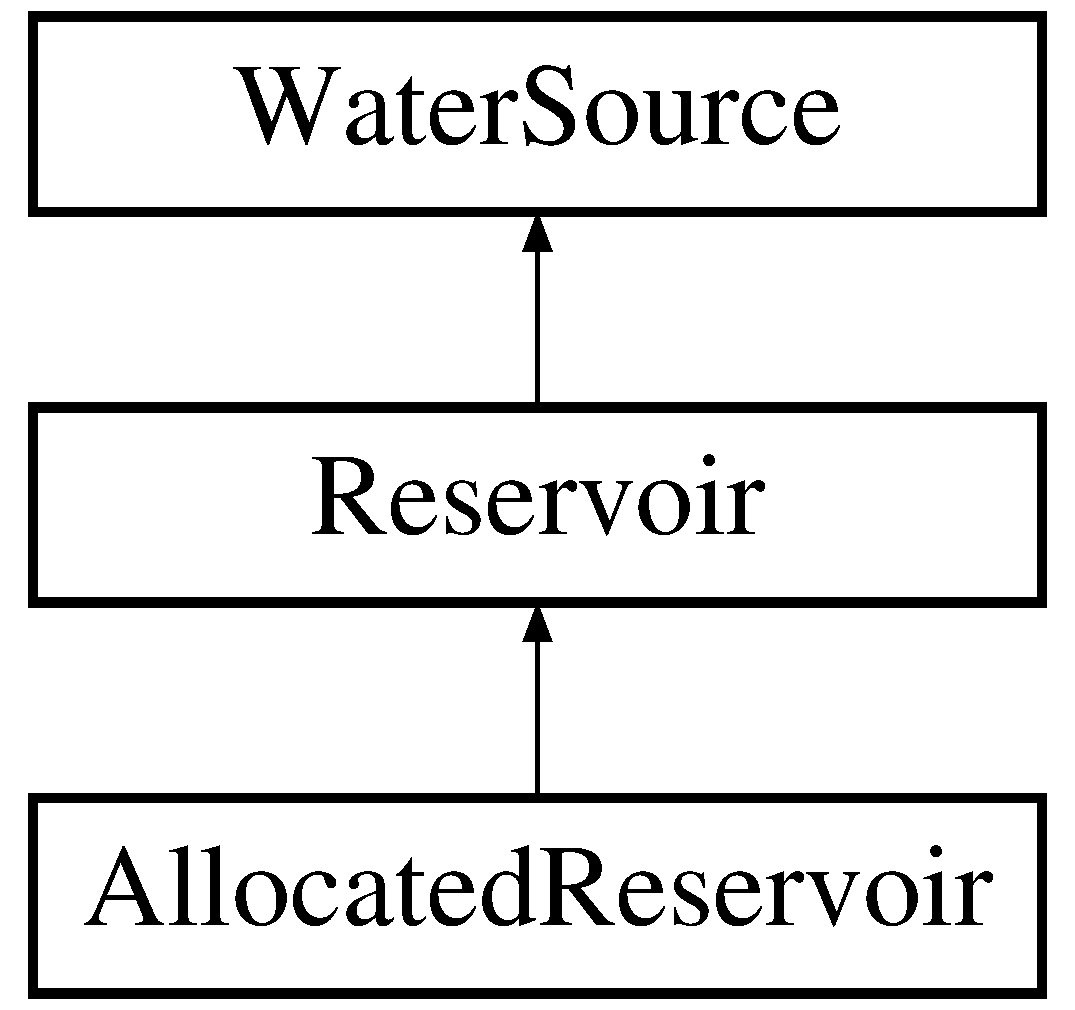
\includegraphics[height=3.000000cm]{classAllocatedReservoir}
\end{center}
\end{figure}
\subsection*{Public Member Functions}
\begin{DoxyCompactItemize}
\item 
\mbox{\hyperlink{classAllocatedReservoir_a0b2d620a1d1fe9a9fe053269f35a9a70}{Allocated\+Reservoir}} (const char $\ast$\mbox{\hyperlink{classWaterSource_a846ea74c5b453d014f594d41fee8c765}{name}}, const int \mbox{\hyperlink{classWaterSource_a6eafe5dfefd317877d1244e8a7c6e742}{id}}, const vector$<$ \mbox{\hyperlink{classCatchment}{Catchment}} $\ast$$>$ \&\mbox{\hyperlink{classWaterSource_a8c18c34f23f8a06685c1d12f462ed830}{catchments}}, const double \mbox{\hyperlink{classWaterSource_a2ec257b415b248214a8bce7fc5267723}{capacity}}, const double max\+\_\+treatment\+\_\+capacity, \mbox{\hyperlink{classEvaporationSeries}{Evaporation\+Series}} \&\mbox{\hyperlink{classReservoir_a2d2d9b302c13703309bb798d24136810}{evaporation\+\_\+series}}, \mbox{\hyperlink{classDataSeries}{Data\+Series}} $\ast$\mbox{\hyperlink{classReservoir_a46bd5b750963dfa9a57b247fd77ab8ff}{storage\+\_\+area\+\_\+curve}}, vector$<$ int $>$ $\ast$\mbox{\hyperlink{classWaterSource_ac345583fc2d0f7e1db31ee40244d7ace}{utilities\+\_\+with\+\_\+allocations}}, vector$<$ double $>$ $\ast$\mbox{\hyperlink{classWaterSource_a2f6655a80c4847fe039987255d9d998c}{allocated\+\_\+fractions}}, vector$<$ double $>$ $\ast$\mbox{\hyperlink{classWaterSource_aa73fe10cfc6579b2fb79529e1dde5140}{allocated\+\_\+treatment\+\_\+fractions}})
\item 
\mbox{\hyperlink{classAllocatedReservoir_a22794afc1f06d13fc3099015a2250b0d}{Allocated\+Reservoir}} (const char $\ast$\mbox{\hyperlink{classWaterSource_a846ea74c5b453d014f594d41fee8c765}{name}}, const int \mbox{\hyperlink{classWaterSource_a6eafe5dfefd317877d1244e8a7c6e742}{id}}, const vector$<$ \mbox{\hyperlink{classCatchment}{Catchment}} $\ast$$>$ \&\mbox{\hyperlink{classWaterSource_a8c18c34f23f8a06685c1d12f462ed830}{catchments}}, const double \mbox{\hyperlink{classWaterSource_a2ec257b415b248214a8bce7fc5267723}{capacity}}, const double max\+\_\+treatment\+\_\+capacity, \mbox{\hyperlink{classEvaporationSeries}{Evaporation\+Series}} \&\mbox{\hyperlink{classReservoir_a2d2d9b302c13703309bb798d24136810}{evaporation\+\_\+series}}, \mbox{\hyperlink{classDataSeries}{Data\+Series}} $\ast$\mbox{\hyperlink{classReservoir_a46bd5b750963dfa9a57b247fd77ab8ff}{storage\+\_\+area\+\_\+curve}}, const vector$<$ double $>$ \&construction\+\_\+time\+\_\+range, double permitting\+\_\+period, \mbox{\hyperlink{classBond}{Bond}} \&bond, vector$<$ int $>$ $\ast$\mbox{\hyperlink{classWaterSource_ac345583fc2d0f7e1db31ee40244d7ace}{utilities\+\_\+with\+\_\+allocations}}, vector$<$ double $>$ $\ast$\mbox{\hyperlink{classWaterSource_a2f6655a80c4847fe039987255d9d998c}{allocated\+\_\+fractions}}, vector$<$ double $>$ $\ast$\mbox{\hyperlink{classWaterSource_aa73fe10cfc6579b2fb79529e1dde5140}{allocated\+\_\+treatment\+\_\+fractions}})
\item 
\mbox{\hyperlink{classAllocatedReservoir_a17a60d40d936b1a68459d0bd9578aada}{Allocated\+Reservoir}} (const char $\ast$\mbox{\hyperlink{classWaterSource_a846ea74c5b453d014f594d41fee8c765}{name}}, const int \mbox{\hyperlink{classWaterSource_a6eafe5dfefd317877d1244e8a7c6e742}{id}}, const vector$<$ \mbox{\hyperlink{classCatchment}{Catchment}} $\ast$$>$ \&\mbox{\hyperlink{classWaterSource_a8c18c34f23f8a06685c1d12f462ed830}{catchments}}, const double \mbox{\hyperlink{classWaterSource_a2ec257b415b248214a8bce7fc5267723}{capacity}}, const double max\+\_\+treatment\+\_\+capacity, \mbox{\hyperlink{classEvaporationSeries}{Evaporation\+Series}} \&\mbox{\hyperlink{classReservoir_a2d2d9b302c13703309bb798d24136810}{evaporation\+\_\+series}}, double storage\+\_\+area, vector$<$ int $>$ $\ast$\mbox{\hyperlink{classWaterSource_ac345583fc2d0f7e1db31ee40244d7ace}{utilities\+\_\+with\+\_\+allocations}}, vector$<$ double $>$ $\ast$\mbox{\hyperlink{classWaterSource_a2f6655a80c4847fe039987255d9d998c}{allocated\+\_\+fractions}}, vector$<$ double $>$ $\ast$\mbox{\hyperlink{classWaterSource_aa73fe10cfc6579b2fb79529e1dde5140}{allocated\+\_\+treatment\+\_\+fractions}})
\item 
\mbox{\hyperlink{classAllocatedReservoir_a44ac982717a21a0b24bb3019d07ffe89}{Allocated\+Reservoir}} (const char $\ast$\mbox{\hyperlink{classWaterSource_a846ea74c5b453d014f594d41fee8c765}{name}}, const int \mbox{\hyperlink{classWaterSource_a6eafe5dfefd317877d1244e8a7c6e742}{id}}, const vector$<$ \mbox{\hyperlink{classCatchment}{Catchment}} $\ast$$>$ \&\mbox{\hyperlink{classWaterSource_a8c18c34f23f8a06685c1d12f462ed830}{catchments}}, const double \mbox{\hyperlink{classWaterSource_a2ec257b415b248214a8bce7fc5267723}{capacity}}, const double max\+\_\+treatment\+\_\+capacity, \mbox{\hyperlink{classEvaporationSeries}{Evaporation\+Series}} \&\mbox{\hyperlink{classReservoir_a2d2d9b302c13703309bb798d24136810}{evaporation\+\_\+series}}, double storage\+\_\+area, const vector$<$ double $>$ \&construction\+\_\+time\+\_\+range, double permitting\+\_\+period, \mbox{\hyperlink{classBond}{Bond}} \&bond, vector$<$ int $>$ $\ast$\mbox{\hyperlink{classWaterSource_ac345583fc2d0f7e1db31ee40244d7ace}{utilities\+\_\+with\+\_\+allocations}}, vector$<$ double $>$ $\ast$\mbox{\hyperlink{classWaterSource_a2f6655a80c4847fe039987255d9d998c}{allocated\+\_\+fractions}}, vector$<$ double $>$ $\ast$\mbox{\hyperlink{classWaterSource_aa73fe10cfc6579b2fb79529e1dde5140}{allocated\+\_\+treatment\+\_\+fractions}})
\item 
\mbox{\hyperlink{classAllocatedReservoir}{Allocated\+Reservoir}} \& \mbox{\hyperlink{classAllocatedReservoir_a83551e53169014906ce7380005efb4f8}{operator=}} (const \mbox{\hyperlink{classAllocatedReservoir}{Allocated\+Reservoir}} \&allocated\+\_\+reservoir)
\item 
\mbox{\hyperlink{classAllocatedReservoir_a59098eb446ada7a23e914543f3c419c0}{Allocated\+Reservoir}} (const \mbox{\hyperlink{classAllocatedReservoir}{Allocated\+Reservoir}} \&allocated\+\_\+reservoir)
\item 
\mbox{\hyperlink{classAllocatedReservoir_a3fc9aaca619a97d338449384e579900c}{$\sim$\+Allocated\+Reservoir}} ()
\item 
void \mbox{\hyperlink{classAllocatedReservoir_aa5a3683ac3a1e7a778627332c6a7fff7}{apply\+Continuity}} (int week, double \mbox{\hyperlink{classWaterSource_a7a69b2e9b6030f1035e6cf44d2918ee5}{upstream\+\_\+source\+\_\+inflow}}, double \mbox{\hyperlink{classWaterSource_aeb5a2d2d83383a70ca20f3e94635a9c7}{wastewater\+\_\+inflow}}, vector$<$ double $>$ \&demand\+\_\+outflow) override
\item 
void \mbox{\hyperlink{classAllocatedReservoir_aea294cbca1e1630a1307072632d14b05}{set\+Full}} () override
\item 
double \mbox{\hyperlink{classAllocatedReservoir_ae161ebfc285aa69cb8b7f4fe20ee7a2e}{get\+Available\+Allocated\+Volume}} (int utility\+\_\+id) override
\item 
void \mbox{\hyperlink{classAllocatedReservoir_a3a9b7ce2e1d42cc373095cfd40ef2ae2}{remove\+Water}} (int allocation\+\_\+id, double volume) override
\item 
double \mbox{\hyperlink{classAllocatedReservoir_a8b9b38494fa23f0bea78134c82644bf1}{get\+Allocated\+Capacity}} (int utility\+\_\+id) override
\item 
double \mbox{\hyperlink{classAllocatedReservoir_a731381982c9245b0bf24db4082dc74c1}{get\+Allocated\+Fraction}} (int utility\+\_\+id) override
\item 
void \mbox{\hyperlink{classAllocatedReservoir_ab4cd10b1a9b421309844bcec42899b70}{add\+Capacity}} (double \mbox{\hyperlink{classWaterSource_a2ec257b415b248214a8bce7fc5267723}{capacity}}) override
\item 
void \mbox{\hyperlink{classAllocatedReservoir_ab781bee3253277f1dcfa4c12756d9d6f}{add\+Treatment\+Capacity}} (const double added\+\_\+plant\+\_\+treatment\+\_\+capacity, int utility\+\_\+id) override
\item 
double \mbox{\hyperlink{classAllocatedReservoir_aba81b93e1aa1154ce411248903fabde6}{get\+Allocated\+Treatment\+Capacity}} (int utility\+\_\+id) const override
\item 
double \mbox{\hyperlink{classAllocatedReservoir_a114e9cde6a106b786ca0ed39283cbbed}{get\+Supply\+Allocated\+Fraction}} (int utility\+\_\+id) override
\item 
bool \mbox{\hyperlink{classAllocatedReservoir_a9d025365aa42dfff13a0aac8ea7863fa}{mass\+\_\+balance\+\_\+with\+\_\+wq\+\_\+pool}} (double net\+\_\+inflow, vector$<$ double $>$ \&demand\+\_\+outflow)
\item 
bool \mbox{\hyperlink{classAllocatedReservoir_ac719b30d5a83ba19ea722449ce9580e1}{mass\+\_\+balance\+\_\+without\+\_\+wq\+\_\+pool}} (double net\+\_\+inflow, vector$<$ double $>$ \&demand\+\_\+outflow)
\item 
void \mbox{\hyperlink{classAllocatedReservoir_a739d93f7981f597a3db0a3d613304b8e}{set\+Online}} () override
\end{DoxyCompactItemize}
\subsection*{Protected Attributes}
\begin{DoxyCompactItemize}
\item 
const bool \mbox{\hyperlink{classAllocatedReservoir_af6a1924f60de19b7f77781af0419c39b}{has\+\_\+water\+\_\+quality\+\_\+pool}}
\item 
double \mbox{\hyperlink{classAllocatedReservoir_ae34d7123ff096d676609e32ba4b83e47}{continuity\+\_\+error}}
\end{DoxyCompactItemize}
\subsection*{Additional Inherited Members}


\subsection{Constructor \& Destructor Documentation}
\mbox{\Hypertarget{classAllocatedReservoir_a0b2d620a1d1fe9a9fe053269f35a9a70}\label{classAllocatedReservoir_a0b2d620a1d1fe9a9fe053269f35a9a70}} 
\index{Allocated\+Reservoir@{Allocated\+Reservoir}!Allocated\+Reservoir@{Allocated\+Reservoir}}
\index{Allocated\+Reservoir@{Allocated\+Reservoir}!Allocated\+Reservoir@{Allocated\+Reservoir}}
\subsubsection{\texorpdfstring{Allocated\+Reservoir()}{AllocatedReservoir()}\hspace{0.1cm}{\footnotesize\ttfamily [1/5]}}
{\footnotesize\ttfamily Allocated\+Reservoir\+::\+Allocated\+Reservoir (\begin{DoxyParamCaption}\item[{const char $\ast$}]{name,  }\item[{const int}]{id,  }\item[{const vector$<$ \mbox{\hyperlink{classCatchment}{Catchment}} $\ast$$>$ \&}]{catchments,  }\item[{const double}]{capacity,  }\item[{const double}]{max\+\_\+treatment\+\_\+capacity,  }\item[{\mbox{\hyperlink{classEvaporationSeries}{Evaporation\+Series}} \&}]{evaporation\+\_\+series,  }\item[{\mbox{\hyperlink{classDataSeries}{Data\+Series}} $\ast$}]{storage\+\_\+area\+\_\+curve,  }\item[{vector$<$ int $>$ $\ast$}]{utilities\+\_\+with\+\_\+allocations,  }\item[{vector$<$ double $>$ $\ast$}]{allocated\+\_\+fractions,  }\item[{vector$<$ double $>$ $\ast$}]{allocated\+\_\+treatment\+\_\+fractions }\end{DoxyParamCaption})}

\mbox{\Hypertarget{classAllocatedReservoir_a22794afc1f06d13fc3099015a2250b0d}\label{classAllocatedReservoir_a22794afc1f06d13fc3099015a2250b0d}} 
\index{Allocated\+Reservoir@{Allocated\+Reservoir}!Allocated\+Reservoir@{Allocated\+Reservoir}}
\index{Allocated\+Reservoir@{Allocated\+Reservoir}!Allocated\+Reservoir@{Allocated\+Reservoir}}
\subsubsection{\texorpdfstring{Allocated\+Reservoir()}{AllocatedReservoir()}\hspace{0.1cm}{\footnotesize\ttfamily [2/5]}}
{\footnotesize\ttfamily Allocated\+Reservoir\+::\+Allocated\+Reservoir (\begin{DoxyParamCaption}\item[{const char $\ast$}]{name,  }\item[{const int}]{id,  }\item[{const vector$<$ \mbox{\hyperlink{classCatchment}{Catchment}} $\ast$$>$ \&}]{catchments,  }\item[{const double}]{capacity,  }\item[{const double}]{max\+\_\+treatment\+\_\+capacity,  }\item[{\mbox{\hyperlink{classEvaporationSeries}{Evaporation\+Series}} \&}]{evaporation\+\_\+series,  }\item[{\mbox{\hyperlink{classDataSeries}{Data\+Series}} $\ast$}]{storage\+\_\+area\+\_\+curve,  }\item[{const vector$<$ double $>$ \&}]{construction\+\_\+time\+\_\+range,  }\item[{double}]{permitting\+\_\+period,  }\item[{\mbox{\hyperlink{classBond}{Bond}} \&}]{bond,  }\item[{vector$<$ int $>$ $\ast$}]{utilities\+\_\+with\+\_\+allocations,  }\item[{vector$<$ double $>$ $\ast$}]{allocated\+\_\+fractions,  }\item[{vector$<$ double $>$ $\ast$}]{allocated\+\_\+treatment\+\_\+fractions }\end{DoxyParamCaption})}

\mbox{\Hypertarget{classAllocatedReservoir_a17a60d40d936b1a68459d0bd9578aada}\label{classAllocatedReservoir_a17a60d40d936b1a68459d0bd9578aada}} 
\index{Allocated\+Reservoir@{Allocated\+Reservoir}!Allocated\+Reservoir@{Allocated\+Reservoir}}
\index{Allocated\+Reservoir@{Allocated\+Reservoir}!Allocated\+Reservoir@{Allocated\+Reservoir}}
\subsubsection{\texorpdfstring{Allocated\+Reservoir()}{AllocatedReservoir()}\hspace{0.1cm}{\footnotesize\ttfamily [3/5]}}
{\footnotesize\ttfamily Allocated\+Reservoir\+::\+Allocated\+Reservoir (\begin{DoxyParamCaption}\item[{const char $\ast$}]{name,  }\item[{const int}]{id,  }\item[{const vector$<$ \mbox{\hyperlink{classCatchment}{Catchment}} $\ast$$>$ \&}]{catchments,  }\item[{const double}]{capacity,  }\item[{const double}]{max\+\_\+treatment\+\_\+capacity,  }\item[{\mbox{\hyperlink{classEvaporationSeries}{Evaporation\+Series}} \&}]{evaporation\+\_\+series,  }\item[{double}]{storage\+\_\+area,  }\item[{vector$<$ int $>$ $\ast$}]{utilities\+\_\+with\+\_\+allocations,  }\item[{vector$<$ double $>$ $\ast$}]{allocated\+\_\+fractions,  }\item[{vector$<$ double $>$ $\ast$}]{allocated\+\_\+treatment\+\_\+fractions }\end{DoxyParamCaption})}

\mbox{\Hypertarget{classAllocatedReservoir_a44ac982717a21a0b24bb3019d07ffe89}\label{classAllocatedReservoir_a44ac982717a21a0b24bb3019d07ffe89}} 
\index{Allocated\+Reservoir@{Allocated\+Reservoir}!Allocated\+Reservoir@{Allocated\+Reservoir}}
\index{Allocated\+Reservoir@{Allocated\+Reservoir}!Allocated\+Reservoir@{Allocated\+Reservoir}}
\subsubsection{\texorpdfstring{Allocated\+Reservoir()}{AllocatedReservoir()}\hspace{0.1cm}{\footnotesize\ttfamily [4/5]}}
{\footnotesize\ttfamily Allocated\+Reservoir\+::\+Allocated\+Reservoir (\begin{DoxyParamCaption}\item[{const char $\ast$}]{name,  }\item[{const int}]{id,  }\item[{const vector$<$ \mbox{\hyperlink{classCatchment}{Catchment}} $\ast$$>$ \&}]{catchments,  }\item[{const double}]{capacity,  }\item[{const double}]{max\+\_\+treatment\+\_\+capacity,  }\item[{\mbox{\hyperlink{classEvaporationSeries}{Evaporation\+Series}} \&}]{evaporation\+\_\+series,  }\item[{double}]{storage\+\_\+area,  }\item[{const vector$<$ double $>$ \&}]{construction\+\_\+time\+\_\+range,  }\item[{double}]{permitting\+\_\+period,  }\item[{\mbox{\hyperlink{classBond}{Bond}} \&}]{bond,  }\item[{vector$<$ int $>$ $\ast$}]{utilities\+\_\+with\+\_\+allocations,  }\item[{vector$<$ double $>$ $\ast$}]{allocated\+\_\+fractions,  }\item[{vector$<$ double $>$ $\ast$}]{allocated\+\_\+treatment\+\_\+fractions }\end{DoxyParamCaption})}

\mbox{\Hypertarget{classAllocatedReservoir_a59098eb446ada7a23e914543f3c419c0}\label{classAllocatedReservoir_a59098eb446ada7a23e914543f3c419c0}} 
\index{Allocated\+Reservoir@{Allocated\+Reservoir}!Allocated\+Reservoir@{Allocated\+Reservoir}}
\index{Allocated\+Reservoir@{Allocated\+Reservoir}!Allocated\+Reservoir@{Allocated\+Reservoir}}
\subsubsection{\texorpdfstring{Allocated\+Reservoir()}{AllocatedReservoir()}\hspace{0.1cm}{\footnotesize\ttfamily [5/5]}}
{\footnotesize\ttfamily Allocated\+Reservoir\+::\+Allocated\+Reservoir (\begin{DoxyParamCaption}\item[{const \mbox{\hyperlink{classAllocatedReservoir}{Allocated\+Reservoir}} \&}]{allocated\+\_\+reservoir }\end{DoxyParamCaption})}

\mbox{\Hypertarget{classAllocatedReservoir_a3fc9aaca619a97d338449384e579900c}\label{classAllocatedReservoir_a3fc9aaca619a97d338449384e579900c}} 
\index{Allocated\+Reservoir@{Allocated\+Reservoir}!````~Allocated\+Reservoir@{$\sim$\+Allocated\+Reservoir}}
\index{````~Allocated\+Reservoir@{$\sim$\+Allocated\+Reservoir}!Allocated\+Reservoir@{Allocated\+Reservoir}}
\subsubsection{\texorpdfstring{$\sim$\+Allocated\+Reservoir()}{~AllocatedReservoir()}}
{\footnotesize\ttfamily Allocated\+Reservoir\+::$\sim$\+Allocated\+Reservoir (\begin{DoxyParamCaption}{ }\end{DoxyParamCaption})\hspace{0.3cm}{\ttfamily [default]}}



\subsection{Member Function Documentation}
\mbox{\Hypertarget{classAllocatedReservoir_ab4cd10b1a9b421309844bcec42899b70}\label{classAllocatedReservoir_ab4cd10b1a9b421309844bcec42899b70}} 
\index{Allocated\+Reservoir@{Allocated\+Reservoir}!add\+Capacity@{add\+Capacity}}
\index{add\+Capacity@{add\+Capacity}!Allocated\+Reservoir@{Allocated\+Reservoir}}
\subsubsection{\texorpdfstring{add\+Capacity()}{addCapacity()}}
{\footnotesize\ttfamily void Allocated\+Reservoir\+::add\+Capacity (\begin{DoxyParamCaption}\item[{double}]{capacity }\end{DoxyParamCaption})\hspace{0.3cm}{\ttfamily [override]}, {\ttfamily [virtual]}}



Reimplemented from \mbox{\hyperlink{classWaterSource_abffedb6e58620b1b1d6f3c4b4480d3a0}{Water\+Source}}.

\mbox{\Hypertarget{classAllocatedReservoir_ab781bee3253277f1dcfa4c12756d9d6f}\label{classAllocatedReservoir_ab781bee3253277f1dcfa4c12756d9d6f}} 
\index{Allocated\+Reservoir@{Allocated\+Reservoir}!add\+Treatment\+Capacity@{add\+Treatment\+Capacity}}
\index{add\+Treatment\+Capacity@{add\+Treatment\+Capacity}!Allocated\+Reservoir@{Allocated\+Reservoir}}
\subsubsection{\texorpdfstring{add\+Treatment\+Capacity()}{addTreatmentCapacity()}}
{\footnotesize\ttfamily void Allocated\+Reservoir\+::add\+Treatment\+Capacity (\begin{DoxyParamCaption}\item[{const double}]{added\+\_\+plant\+\_\+treatment\+\_\+capacity,  }\item[{int}]{utility\+\_\+id }\end{DoxyParamCaption})\hspace{0.3cm}{\ttfamily [override]}, {\ttfamily [virtual]}}

Addes treatment capacity to a source. The specification of both the total treatment capacity of the new plant and the fraction of the treatment capacity allocated to a given utility allow for joint treatment plants. To have one utility only building an exclusive plant, the fraction will be 1. 
\begin{DoxyParams}{Parameters}
{\em added\+\_\+plant\+\_\+treatment\+\_\+capacity} & \\
\hline
{\em allocated\+\_\+fraction\+\_\+of\+\_\+total\+\_\+capacity} & \\
\hline
{\em utility\+\_\+id} & \\
\hline
\end{DoxyParams}
Add capacity to respective treatment allocation.

Update treatment allocation fractions based on new allocated amounts and new total treatment capacity. 

Reimplemented from \mbox{\hyperlink{classWaterSource_a210818957f088da4046597d0f1a1340f}{Water\+Source}}.

\mbox{\Hypertarget{classAllocatedReservoir_aa5a3683ac3a1e7a778627332c6a7fff7}\label{classAllocatedReservoir_aa5a3683ac3a1e7a778627332c6a7fff7}} 
\index{Allocated\+Reservoir@{Allocated\+Reservoir}!apply\+Continuity@{apply\+Continuity}}
\index{apply\+Continuity@{apply\+Continuity}!Allocated\+Reservoir@{Allocated\+Reservoir}}
\subsubsection{\texorpdfstring{apply\+Continuity()}{applyContinuity()}}
{\footnotesize\ttfamily void Allocated\+Reservoir\+::apply\+Continuity (\begin{DoxyParamCaption}\item[{int}]{week,  }\item[{double}]{upstream\+\_\+source\+\_\+inflow,  }\item[{double}]{wastewater\+\_\+inflow,  }\item[{vector$<$ double $>$ \&}]{demand\+\_\+outflow }\end{DoxyParamCaption})\hspace{0.3cm}{\ttfamily [override]}, {\ttfamily [virtual]}}

Constrain outflow to what is available on water quality pool.

Calculate total runoff inflow reaching reservoir from its watershed.

Calculates water lost through evaporation.

Calculate new stored volume and outflow based on continuity.

Check if spillage is needed and, if so, correct stored volume and calculate spillage and set all allocations to full. Otherwise, distributed inflows and outflows among respective allocations. ~\newline
~\newline
~\newline
~\newline
~\newline
~\newline
~\newline
~\newline
~\newline
~\newline
~\newline
 Water exceeding allocated capacities.

Volume of water that entered the reservoir and stayed until being used or released. ~\newline
~\newline
~\newline
~\newline
~\newline
~\newline
~\newline
~\newline
~\newline
 Split among utilities any allocated volume exceeding a giver utility\textquotesingle{}s maximum allocated capacity. ~\newline
~\newline
~\newline
~\newline
~\newline
~\newline
~\newline
~\newline
 Calculate combined excess allocation and combined allocation fraction. ~\newline
~\newline
~\newline
~\newline
~\newline
~\newline
~\newline
 Calculation of amount exceeding all individual allocations

Redistribute combined excess among utilities based on their allocation fractions. If one is exceeded, roll \char`\"{}second order\char`\"{} excess down to the next utility. ~\newline
~\newline
~\newline
~\newline
~\newline
 Redistribute excess based on allocations fractions.

Check if redistribution of excesses didn\textquotesingle{}t make an allocation exceed its capacity. ~\newline
~\newline
~\newline
 If there was too much water added to an allocation, redistribute it. ~\newline
~\newline
 If there\textquotesingle{}s still an excess but all allocations are at capacity, release the rest as environmental flows. ~\newline
 Sanity checking from now on. 

Implements \mbox{\hyperlink{classWaterSource_ac070445379fe706f65b977dade4f3fbc}{Water\+Source}}.

\mbox{\Hypertarget{classAllocatedReservoir_a8b9b38494fa23f0bea78134c82644bf1}\label{classAllocatedReservoir_a8b9b38494fa23f0bea78134c82644bf1}} 
\index{Allocated\+Reservoir@{Allocated\+Reservoir}!get\+Allocated\+Capacity@{get\+Allocated\+Capacity}}
\index{get\+Allocated\+Capacity@{get\+Allocated\+Capacity}!Allocated\+Reservoir@{Allocated\+Reservoir}}
\subsubsection{\texorpdfstring{get\+Allocated\+Capacity()}{getAllocatedCapacity()}}
{\footnotesize\ttfamily double Allocated\+Reservoir\+::get\+Allocated\+Capacity (\begin{DoxyParamCaption}\item[{int}]{utility\+\_\+id }\end{DoxyParamCaption})\hspace{0.3cm}{\ttfamily [override]}, {\ttfamily [virtual]}}

Most sources will not have different allocations, so by default this function will return the total capacity. If a source is to have multiple allocations, this function must be overriden to make sure it returns the right value. 
\begin{DoxyParams}{Parameters}
{\em utility\+\_\+id} & \\
\hline
\end{DoxyParams}
\begin{DoxyReturn}{Returns}

\end{DoxyReturn}


Reimplemented from \mbox{\hyperlink{classWaterSource_a44102a0eafdaebd86f0ed8dabb313733}{Water\+Source}}.

\mbox{\Hypertarget{classAllocatedReservoir_a731381982c9245b0bf24db4082dc74c1}\label{classAllocatedReservoir_a731381982c9245b0bf24db4082dc74c1}} 
\index{Allocated\+Reservoir@{Allocated\+Reservoir}!get\+Allocated\+Fraction@{get\+Allocated\+Fraction}}
\index{get\+Allocated\+Fraction@{get\+Allocated\+Fraction}!Allocated\+Reservoir@{Allocated\+Reservoir}}
\subsubsection{\texorpdfstring{get\+Allocated\+Fraction()}{getAllocatedFraction()}}
{\footnotesize\ttfamily double Allocated\+Reservoir\+::get\+Allocated\+Fraction (\begin{DoxyParamCaption}\item[{int}]{utility\+\_\+id }\end{DoxyParamCaption})\hspace{0.3cm}{\ttfamily [override]}, {\ttfamily [virtual]}}



Reimplemented from \mbox{\hyperlink{classWaterSource_a1843ada21b8e7500d80a5a7db10621b3}{Water\+Source}}.

\mbox{\Hypertarget{classAllocatedReservoir_aba81b93e1aa1154ce411248903fabde6}\label{classAllocatedReservoir_aba81b93e1aa1154ce411248903fabde6}} 
\index{Allocated\+Reservoir@{Allocated\+Reservoir}!get\+Allocated\+Treatment\+Capacity@{get\+Allocated\+Treatment\+Capacity}}
\index{get\+Allocated\+Treatment\+Capacity@{get\+Allocated\+Treatment\+Capacity}!Allocated\+Reservoir@{Allocated\+Reservoir}}
\subsubsection{\texorpdfstring{get\+Allocated\+Treatment\+Capacity()}{getAllocatedTreatmentCapacity()}}
{\footnotesize\ttfamily double Allocated\+Reservoir\+::get\+Allocated\+Treatment\+Capacity (\begin{DoxyParamCaption}\item[{int}]{utility\+\_\+id }\end{DoxyParamCaption}) const\hspace{0.3cm}{\ttfamily [override]}, {\ttfamily [virtual]}}



Reimplemented from \mbox{\hyperlink{classWaterSource_ab3ba86d2a3e864e435ba2b88cceea555}{Water\+Source}}.

\mbox{\Hypertarget{classAllocatedReservoir_ae161ebfc285aa69cb8b7f4fe20ee7a2e}\label{classAllocatedReservoir_ae161ebfc285aa69cb8b7f4fe20ee7a2e}} 
\index{Allocated\+Reservoir@{Allocated\+Reservoir}!get\+Available\+Allocated\+Volume@{get\+Available\+Allocated\+Volume}}
\index{get\+Available\+Allocated\+Volume@{get\+Available\+Allocated\+Volume}!Allocated\+Reservoir@{Allocated\+Reservoir}}
\subsubsection{\texorpdfstring{get\+Available\+Allocated\+Volume()}{getAvailableAllocatedVolume()}}
{\footnotesize\ttfamily double Allocated\+Reservoir\+::get\+Available\+Allocated\+Volume (\begin{DoxyParamCaption}\item[{int}]{utility\+\_\+id }\end{DoxyParamCaption})\hspace{0.3cm}{\ttfamily [override]}, {\ttfamily [virtual]}}

If creating a new water source that can be allocated to different utilities, this function must be overwritten to\+: return available\+\_\+allocated\+\_\+volumes\mbox{[}utility\+\_\+id\mbox{]}; 
\begin{DoxyParams}{Parameters}
{\em utility\+\_\+id} & \\
\hline
\end{DoxyParams}
\begin{DoxyReturn}{Returns}

\end{DoxyReturn}


Reimplemented from \mbox{\hyperlink{classWaterSource_a42c687a3be3d88ba38dbea668c8d35cf}{Water\+Source}}.

\mbox{\Hypertarget{classAllocatedReservoir_a114e9cde6a106b786ca0ed39283cbbed}\label{classAllocatedReservoir_a114e9cde6a106b786ca0ed39283cbbed}} 
\index{Allocated\+Reservoir@{Allocated\+Reservoir}!get\+Supply\+Allocated\+Fraction@{get\+Supply\+Allocated\+Fraction}}
\index{get\+Supply\+Allocated\+Fraction@{get\+Supply\+Allocated\+Fraction}!Allocated\+Reservoir@{Allocated\+Reservoir}}
\subsubsection{\texorpdfstring{get\+Supply\+Allocated\+Fraction()}{getSupplyAllocatedFraction()}}
{\footnotesize\ttfamily double Allocated\+Reservoir\+::get\+Supply\+Allocated\+Fraction (\begin{DoxyParamCaption}\item[{int}]{utility\+\_\+id }\end{DoxyParamCaption})\hspace{0.3cm}{\ttfamily [override]}, {\ttfamily [virtual]}}



Reimplemented from \mbox{\hyperlink{classWaterSource_a71cb8bd481bbce0089aa78dcd1c3309a}{Water\+Source}}.

\mbox{\Hypertarget{classAllocatedReservoir_a9d025365aa42dfff13a0aac8ea7863fa}\label{classAllocatedReservoir_a9d025365aa42dfff13a0aac8ea7863fa}} 
\index{Allocated\+Reservoir@{Allocated\+Reservoir}!mass\+\_\+balance\+\_\+with\+\_\+wq\+\_\+pool@{mass\+\_\+balance\+\_\+with\+\_\+wq\+\_\+pool}}
\index{mass\+\_\+balance\+\_\+with\+\_\+wq\+\_\+pool@{mass\+\_\+balance\+\_\+with\+\_\+wq\+\_\+pool}!Allocated\+Reservoir@{Allocated\+Reservoir}}
\subsubsection{\texorpdfstring{mass\+\_\+balance\+\_\+with\+\_\+wq\+\_\+pool()}{mass\_balance\_with\_wq\_pool()}}
{\footnotesize\ttfamily bool Allocated\+Reservoir\+::mass\+\_\+balance\+\_\+with\+\_\+wq\+\_\+pool (\begin{DoxyParamCaption}\item[{double}]{net\+\_\+inflow,  }\item[{vector$<$ double $>$ \&}]{demand\+\_\+outflow }\end{DoxyParamCaption})}

Split inflows and evaporation among allocations and subtract demands. ~\newline
~\newline
~\newline
~\newline
~\newline
 Flag the occurrence of an allocation exceeding its capacity

If allocated volume gets negative for any utility, charge that consumption (basically evaporation) to the water quality pool. Improvements can be made to this, but it may make code significantly slower.

the water quality pool has no demand but provides the minimum environmental flows. ~\newline
~\newline
 Flag the occurrence of an allocation exceeding its capacity

Get water from water quality pool for supply. Check continuity for errors. \mbox{\Hypertarget{classAllocatedReservoir_ac719b30d5a83ba19ea722449ce9580e1}\label{classAllocatedReservoir_ac719b30d5a83ba19ea722449ce9580e1}} 
\index{Allocated\+Reservoir@{Allocated\+Reservoir}!mass\+\_\+balance\+\_\+without\+\_\+wq\+\_\+pool@{mass\+\_\+balance\+\_\+without\+\_\+wq\+\_\+pool}}
\index{mass\+\_\+balance\+\_\+without\+\_\+wq\+\_\+pool@{mass\+\_\+balance\+\_\+without\+\_\+wq\+\_\+pool}!Allocated\+Reservoir@{Allocated\+Reservoir}}
\subsubsection{\texorpdfstring{mass\+\_\+balance\+\_\+without\+\_\+wq\+\_\+pool()}{mass\_balance\_without\_wq\_pool()}}
{\footnotesize\ttfamily bool Allocated\+Reservoir\+::mass\+\_\+balance\+\_\+without\+\_\+wq\+\_\+pool (\begin{DoxyParamCaption}\item[{double}]{net\+\_\+inflow,  }\item[{vector$<$ double $>$ \&}]{demand\+\_\+outflow }\end{DoxyParamCaption})}

Split inflows, min environmental outflows and evaporation among allocations and subtract demands. ~\newline
 Flag the occurrence of an allocation exceeding its capacity \mbox{\Hypertarget{classAllocatedReservoir_a83551e53169014906ce7380005efb4f8}\label{classAllocatedReservoir_a83551e53169014906ce7380005efb4f8}} 
\index{Allocated\+Reservoir@{Allocated\+Reservoir}!operator=@{operator=}}
\index{operator=@{operator=}!Allocated\+Reservoir@{Allocated\+Reservoir}}
\subsubsection{\texorpdfstring{operator=()}{operator=()}}
{\footnotesize\ttfamily \mbox{\hyperlink{classAllocatedReservoir}{Allocated\+Reservoir}} \& Allocated\+Reservoir\+::operator= (\begin{DoxyParamCaption}\item[{const \mbox{\hyperlink{classAllocatedReservoir}{Allocated\+Reservoir}} \&}]{allocated\+\_\+reservoir }\end{DoxyParamCaption})}

Copy assignment operator 
\begin{DoxyParams}{Parameters}
{\em allocated\+\_\+reservoir} & \\
\hline
\end{DoxyParams}
\begin{DoxyReturn}{Returns}

\end{DoxyReturn}
\mbox{\Hypertarget{classAllocatedReservoir_a3a9b7ce2e1d42cc373095cfd40ef2ae2}\label{classAllocatedReservoir_a3a9b7ce2e1d42cc373095cfd40ef2ae2}} 
\index{Allocated\+Reservoir@{Allocated\+Reservoir}!remove\+Water@{remove\+Water}}
\index{remove\+Water@{remove\+Water}!Allocated\+Reservoir@{Allocated\+Reservoir}}
\subsubsection{\texorpdfstring{remove\+Water()}{removeWater()}}
{\footnotesize\ttfamily void Allocated\+Reservoir\+::remove\+Water (\begin{DoxyParamCaption}\item[{int}]{allocation\+\_\+id,  }\item[{double}]{volume }\end{DoxyParamCaption})\hspace{0.3cm}{\ttfamily [override]}, {\ttfamily [virtual]}}

If creating a new water source that can be allocated to different utilities, this function must be overwritten to\+: available\+\_\+allocated\+\_\+volumes\mbox{[}allocation\+\_\+id\mbox{]} -\/= volume; available\+\_\+volume -\/= volume; demand += volume; 
\begin{DoxyParams}{Parameters}
{\em utility\+\_\+id} & \\
\hline
\end{DoxyParams}
\begin{DoxyReturn}{Returns}

\end{DoxyReturn}


Reimplemented from \mbox{\hyperlink{classWaterSource_ab697c3a0765d445f72533f6a5f139bd9}{Water\+Source}}.

\mbox{\Hypertarget{classAllocatedReservoir_aea294cbca1e1630a1307072632d14b05}\label{classAllocatedReservoir_aea294cbca1e1630a1307072632d14b05}} 
\index{Allocated\+Reservoir@{Allocated\+Reservoir}!set\+Full@{set\+Full}}
\index{set\+Full@{set\+Full}!Allocated\+Reservoir@{Allocated\+Reservoir}}
\subsubsection{\texorpdfstring{set\+Full()}{setFull()}}
{\footnotesize\ttfamily void Allocated\+Reservoir\+::set\+Full (\begin{DoxyParamCaption}{ }\end{DoxyParamCaption})\hspace{0.3cm}{\ttfamily [override]}, {\ttfamily [virtual]}}



Reimplemented from \mbox{\hyperlink{classWaterSource_a5f8007eb1ae604cfaa67ebb4c0c46eb1}{Water\+Source}}.

\mbox{\Hypertarget{classAllocatedReservoir_a739d93f7981f597a3db0a3d613304b8e}\label{classAllocatedReservoir_a739d93f7981f597a3db0a3d613304b8e}} 
\index{Allocated\+Reservoir@{Allocated\+Reservoir}!set\+Online@{set\+Online}}
\index{set\+Online@{set\+Online}!Allocated\+Reservoir@{Allocated\+Reservoir}}
\subsubsection{\texorpdfstring{set\+Online()}{setOnline()}}
{\footnotesize\ttfamily void Allocated\+Reservoir\+::set\+Online (\begin{DoxyParamCaption}{ }\end{DoxyParamCaption})\hspace{0.3cm}{\ttfamily [override]}, {\ttfamily [virtual]}}

start empty and gradually fill as inflows start coming in.

set all allocated volumes to zero 

Reimplemented from \mbox{\hyperlink{classWaterSource_ab3396e2915db91a6c82e0f29c7889df4}{Water\+Source}}.



\subsection{Member Data Documentation}
\mbox{\Hypertarget{classAllocatedReservoir_ae34d7123ff096d676609e32ba4b83e47}\label{classAllocatedReservoir_ae34d7123ff096d676609e32ba4b83e47}} 
\index{Allocated\+Reservoir@{Allocated\+Reservoir}!continuity\+\_\+error@{continuity\+\_\+error}}
\index{continuity\+\_\+error@{continuity\+\_\+error}!Allocated\+Reservoir@{Allocated\+Reservoir}}
\subsubsection{\texorpdfstring{continuity\+\_\+error}{continuity\_error}}
{\footnotesize\ttfamily double Allocated\+Reservoir\+::continuity\+\_\+error\hspace{0.3cm}{\ttfamily [protected]}}

\mbox{\Hypertarget{classAllocatedReservoir_af6a1924f60de19b7f77781af0419c39b}\label{classAllocatedReservoir_af6a1924f60de19b7f77781af0419c39b}} 
\index{Allocated\+Reservoir@{Allocated\+Reservoir}!has\+\_\+water\+\_\+quality\+\_\+pool@{has\+\_\+water\+\_\+quality\+\_\+pool}}
\index{has\+\_\+water\+\_\+quality\+\_\+pool@{has\+\_\+water\+\_\+quality\+\_\+pool}!Allocated\+Reservoir@{Allocated\+Reservoir}}
\subsubsection{\texorpdfstring{has\+\_\+water\+\_\+quality\+\_\+pool}{has\_water\_quality\_pool}}
{\footnotesize\ttfamily const bool Allocated\+Reservoir\+::has\+\_\+water\+\_\+quality\+\_\+pool\hspace{0.3cm}{\ttfamily [protected]}}



The documentation for this class was generated from the following files\+:\begin{DoxyCompactItemize}
\item 
src/\+System\+Components/\+Water\+Sources/\mbox{\hyperlink{AllocatedReservoir_8h}{Allocated\+Reservoir.\+h}}\item 
src/\+System\+Components/\+Water\+Sources/\mbox{\hyperlink{AllocatedReservoir_8cpp}{Allocated\+Reservoir.\+cpp}}\end{DoxyCompactItemize}

\hypertarget{classBalloonPaymentBond}{}\section{Balloon\+Payment\+Bond Class Reference}
\label{classBalloonPaymentBond}\index{Balloon\+Payment\+Bond@{Balloon\+Payment\+Bond}}


The {\ttfamily \mbox{\hyperlink{classBalloonPaymentBond}{Balloon\+Payment\+Bond}}} class is a subclass of the main {\ttfamily \mbox{\hyperlink{classBond}{Bond}}} class. This class that represents a balloon bond that pays interest for a number of years and then pays the face value of the bond plus the last interest payment.  




{\ttfamily \#include $<$Balloon\+Payment\+Bond.\+h$>$}

Inheritance diagram for Balloon\+Payment\+Bond\+:\begin{figure}[H]
\begin{center}
\leavevmode
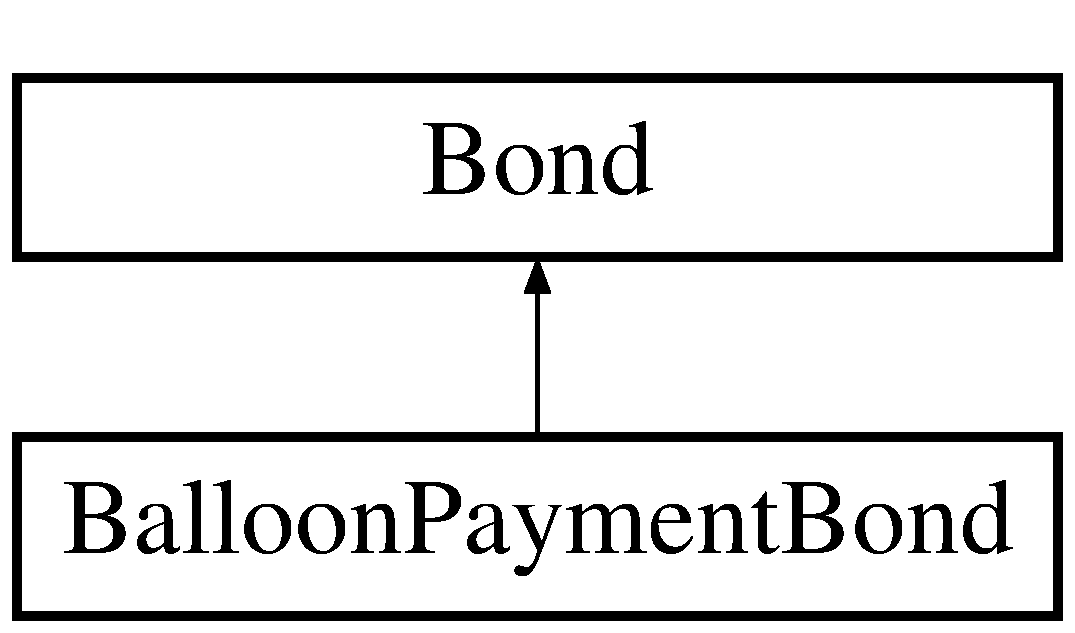
\includegraphics[height=2.000000cm]{classBalloonPaymentBond}
\end{center}
\end{figure}
\subsection*{Public Member Functions}
\begin{DoxyCompactItemize}
\item 
\mbox{\hyperlink{classBalloonPaymentBond_a03b25124896e67f851a35721c37705fe}{Balloon\+Payment\+Bond}} (const int \mbox{\hyperlink{classBond_a7f75bcafbc16676ad6dbafbf40afae4a}{id}}, const double \mbox{\hyperlink{classBond_ad98df7d28b398e620286f95ee085439b}{cost\+\_\+of\+\_\+capital}}, const int \mbox{\hyperlink{classBond_a4a227b6de2eeada118d82ab1633b1db8}{n\+\_\+payments}}, const double \mbox{\hyperlink{classBond_a5f66785534e24caa43d9f730130a6463}{coupon\+\_\+rate}}, vector$<$ int $>$ \mbox{\hyperlink{classBond_ae8dd46fcbf95c993460ffe4ea1f52739}{pay\+\_\+on\+\_\+weeks}})
\begin{DoxyCompactList}\small\item\em Constructs a \mbox{\hyperlink{classBalloonPaymentBond}{Balloon\+Payment\+Bond}} object with specified attributes. This function initializes a balloon payment bond with the provided parameters. \end{DoxyCompactList}\item 
\mbox{\hyperlink{classBalloonPaymentBond_afc8bb53b6642dac9811414b447279e5b}{Balloon\+Payment\+Bond}} (const int \mbox{\hyperlink{classBond_a7f75bcafbc16676ad6dbafbf40afae4a}{id}}, const double \mbox{\hyperlink{classBond_ad98df7d28b398e620286f95ee085439b}{cost\+\_\+of\+\_\+capital}}, const int \mbox{\hyperlink{classBond_a4a227b6de2eeada118d82ab1633b1db8}{n\+\_\+payments}}, const double \mbox{\hyperlink{classBond_a5f66785534e24caa43d9f730130a6463}{coupon\+\_\+rate}}, vector$<$ int $>$ \mbox{\hyperlink{classBond_ae8dd46fcbf95c993460ffe4ea1f52739}{pay\+\_\+on\+\_\+weeks}}, const int begin\+\_\+repayment\+\_\+after\+\_\+n\+\_\+years)
\begin{DoxyCompactList}\small\item\em Constructs a \mbox{\hyperlink{classBalloonPaymentBond}{Balloon\+Payment\+Bond}} object with specified attributes, including the repayment start time. This function initializes a balloon payment bond with the provided parameters, including the number of payments and repayment start time. \end{DoxyCompactList}\item 
double \mbox{\hyperlink{classBalloonPaymentBond_a8648a2ae688f90a3b2e6689711c22b9d}{get\+Debt\+Service}} (int week) override
\begin{DoxyCompactList}\small\item\em Calculates the debt service for a balloon payment bond at a specific week. This function determines whether a payment is due based on the current week and the bond\textquotesingle{}s payment schedule. It returns the debt service, which includes interest payments for the period and the principal payment for the final period. \end{DoxyCompactList}\item 
double \mbox{\hyperlink{classBalloonPaymentBond_ae038863f7a3408c2c8cd503d8e789f2d}{get\+Present\+Value\+Debt\+Service}} (int week, double discount\+\_\+rate) override
\begin{DoxyCompactList}\small\item\em Calculates the present value of the balloon payment bond\textquotesingle{}s debt service for a specific week. This function computes the present value of the bond\textquotesingle{}s debt service based on the interest payments, the principal payment (if due), and the discount rate. \end{DoxyCompactList}\item 
double \mbox{\hyperlink{classBalloonPaymentBond_abbfaae70e003f057ec842d3889138345}{get\+Net\+Present\+Value\+At\+Issuance}} (double yearly\+\_\+discount\+\_\+rate, int week) const override
\begin{DoxyCompactList}\small\item\em Calculates the net present value (N\+PV) of the balloon payment bond at issuance. This function computes the N\+PV of the bond based on the interest payments and the discount rate. The N\+PV is calculated using the bond\textquotesingle{}s payment schedule, adjusting for the time until repayment begins. \end{DoxyCompactList}\item 
void \mbox{\hyperlink{classBalloonPaymentBond_af22552acd74b08dbb1d308cc5e45344c}{issue\+Bond}} (int week, int construction\+\_\+time, double bond\+\_\+term\+\_\+multiplier, double bond\+\_\+interest\+\_\+rate\+\_\+multiplier) override
\begin{DoxyCompactList}\small\item\em Issues the balloon payment bond, initializing the bond parameters and setting the interest payments. This function sets up the bond\textquotesingle{}s issuance details, including adjusting the interest payments based on the bond\textquotesingle{}s parameters. \end{DoxyCompactList}\end{DoxyCompactItemize}
\subsection*{Additional Inherited Members}


\subsection{Detailed Description}
The {\ttfamily \mbox{\hyperlink{classBalloonPaymentBond}{Balloon\+Payment\+Bond}}} class is a subclass of the main {\ttfamily \mbox{\hyperlink{classBond}{Bond}}} class. This class that represents a balloon bond that pays interest for a number of years and then pays the face value of the bond plus the last interest payment. 

Created by bernardo on 4/17/18. 

\subsection{Constructor \& Destructor Documentation}
\mbox{\Hypertarget{classBalloonPaymentBond_a03b25124896e67f851a35721c37705fe}\label{classBalloonPaymentBond_a03b25124896e67f851a35721c37705fe}} 
\index{Balloon\+Payment\+Bond@{Balloon\+Payment\+Bond}!Balloon\+Payment\+Bond@{Balloon\+Payment\+Bond}}
\index{Balloon\+Payment\+Bond@{Balloon\+Payment\+Bond}!Balloon\+Payment\+Bond@{Balloon\+Payment\+Bond}}
\subsubsection{\texorpdfstring{Balloon\+Payment\+Bond()}{BalloonPaymentBond()}\hspace{0.1cm}{\footnotesize\ttfamily [1/2]}}
{\footnotesize\ttfamily Balloon\+Payment\+Bond\+::\+Balloon\+Payment\+Bond (\begin{DoxyParamCaption}\item[{const int}]{id,  }\item[{const double}]{cost\+\_\+of\+\_\+capital,  }\item[{const int}]{n\+\_\+payments,  }\item[{const double}]{coupon\+\_\+rate,  }\item[{vector$<$ int $>$}]{pay\+\_\+on\+\_\+weeks }\end{DoxyParamCaption})}



Constructs a \mbox{\hyperlink{classBalloonPaymentBond}{Balloon\+Payment\+Bond}} object with specified attributes. This function initializes a balloon payment bond with the provided parameters. 


\begin{DoxyParams}{Parameters}
{\em id} & The unique identifier for the bond. \\
\hline
{\em cost\+\_\+of\+\_\+capital} & The cost of capital associated with the bond. Must be non-\/negative. \\
\hline
{\em n\+\_\+payments} & The total number of payments for the bond. \\
\hline
{\em coupon\+\_\+rate} & The fixed coupon rate for the bond. \\
\hline
{\em pay\+\_\+on\+\_\+weeks} & A vector specifying the weeks when payments are due.\\
\hline
\end{DoxyParams}
\begin{DoxyReturn}{Returns}
None 
\end{DoxyReturn}
\mbox{\Hypertarget{classBalloonPaymentBond_afc8bb53b6642dac9811414b447279e5b}\label{classBalloonPaymentBond_afc8bb53b6642dac9811414b447279e5b}} 
\index{Balloon\+Payment\+Bond@{Balloon\+Payment\+Bond}!Balloon\+Payment\+Bond@{Balloon\+Payment\+Bond}}
\index{Balloon\+Payment\+Bond@{Balloon\+Payment\+Bond}!Balloon\+Payment\+Bond@{Balloon\+Payment\+Bond}}
\subsubsection{\texorpdfstring{Balloon\+Payment\+Bond()}{BalloonPaymentBond()}\hspace{0.1cm}{\footnotesize\ttfamily [2/2]}}
{\footnotesize\ttfamily Balloon\+Payment\+Bond\+::\+Balloon\+Payment\+Bond (\begin{DoxyParamCaption}\item[{const int}]{id,  }\item[{const double}]{cost\+\_\+of\+\_\+capital,  }\item[{const int}]{n\+\_\+payments,  }\item[{const double}]{coupon\+\_\+rate,  }\item[{vector$<$ int $>$}]{pay\+\_\+on\+\_\+weeks,  }\item[{const int}]{begin\+\_\+repayment\+\_\+after\+\_\+n\+\_\+years }\end{DoxyParamCaption})}



Constructs a \mbox{\hyperlink{classBalloonPaymentBond}{Balloon\+Payment\+Bond}} object with specified attributes, including the repayment start time. This function initializes a balloon payment bond with the provided parameters, including the number of payments and repayment start time. 


\begin{DoxyParams}{Parameters}
{\em id} & The unique identifier for the bond. \\
\hline
{\em cost\+\_\+of\+\_\+capital} & The cost of capital associated with the bond. Must be non-\/negative. \\
\hline
{\em n\+\_\+payments} & The total number of payments for the bond. \\
\hline
{\em coupon\+\_\+rate} & The fixed coupon rate for the bond. \\
\hline
{\em pay\+\_\+on\+\_\+weeks} & A vector specifying the weeks when payments are due. \\
\hline
{\em begin\+\_\+repayment\+\_\+after\+\_\+n\+\_\+years} & The number of years after which repayment should begin. A value of {\ttfamily N\+O\+NE} indicates no specific start time.\\
\hline
\end{DoxyParams}
\begin{DoxyReturn}{Returns}
None 
\end{DoxyReturn}


\subsection{Member Function Documentation}
\mbox{\Hypertarget{classBalloonPaymentBond_a8648a2ae688f90a3b2e6689711c22b9d}\label{classBalloonPaymentBond_a8648a2ae688f90a3b2e6689711c22b9d}} 
\index{Balloon\+Payment\+Bond@{Balloon\+Payment\+Bond}!get\+Debt\+Service@{get\+Debt\+Service}}
\index{get\+Debt\+Service@{get\+Debt\+Service}!Balloon\+Payment\+Bond@{Balloon\+Payment\+Bond}}
\subsubsection{\texorpdfstring{get\+Debt\+Service()}{getDebtService()}}
{\footnotesize\ttfamily double Balloon\+Payment\+Bond\+::get\+Debt\+Service (\begin{DoxyParamCaption}\item[{int}]{week }\end{DoxyParamCaption})\hspace{0.3cm}{\ttfamily [override]}, {\ttfamily [virtual]}}



Calculates the debt service for a balloon payment bond at a specific week. This function determines whether a payment is due based on the current week and the bond\textquotesingle{}s payment schedule. It returns the debt service, which includes interest payments for the period and the principal payment for the final period. 


\begin{DoxyParams}{Parameters}
{\em week} & The current week for which to calculate the debt service.\\
\hline
\end{DoxyParams}
\begin{DoxyReturn}{Returns}
double The debt service for the given week, including interest payments and principal payment if due. 
\end{DoxyReturn}


Implements \mbox{\hyperlink{classBond_a98d8ecaf4b36319674ebd220598996bc}{Bond}}.

\mbox{\Hypertarget{classBalloonPaymentBond_abbfaae70e003f057ec842d3889138345}\label{classBalloonPaymentBond_abbfaae70e003f057ec842d3889138345}} 
\index{Balloon\+Payment\+Bond@{Balloon\+Payment\+Bond}!get\+Net\+Present\+Value\+At\+Issuance@{get\+Net\+Present\+Value\+At\+Issuance}}
\index{get\+Net\+Present\+Value\+At\+Issuance@{get\+Net\+Present\+Value\+At\+Issuance}!Balloon\+Payment\+Bond@{Balloon\+Payment\+Bond}}
\subsubsection{\texorpdfstring{get\+Net\+Present\+Value\+At\+Issuance()}{getNetPresentValueAtIssuance()}}
{\footnotesize\ttfamily double Balloon\+Payment\+Bond\+::get\+Net\+Present\+Value\+At\+Issuance (\begin{DoxyParamCaption}\item[{double}]{yearly\+\_\+discount\+\_\+rate,  }\item[{int}]{week }\end{DoxyParamCaption}) const\hspace{0.3cm}{\ttfamily [override]}, {\ttfamily [virtual]}}



Calculates the net present value (N\+PV) of the balloon payment bond at issuance. This function computes the N\+PV of the bond based on the interest payments and the discount rate. The N\+PV is calculated using the bond\textquotesingle{}s payment schedule, adjusting for the time until repayment begins. 


\begin{DoxyParams}{Parameters}
{\em yearly\+\_\+discount\+\_\+rate} & The annual discount rate used to calculate the present value of future payments. \\
\hline
{\em week} & The week of the year to calculate the N\+PV for, typically the week the bond is issued.\\
\hline
\end{DoxyParams}
\begin{DoxyReturn}{Returns}
double The net present value at issuance of the balloon payment bond. 
\end{DoxyReturn}


Implements \mbox{\hyperlink{classBond_a5997278813deb16aa5d01bbca8ecc7b2}{Bond}}.

\mbox{\Hypertarget{classBalloonPaymentBond_ae038863f7a3408c2c8cd503d8e789f2d}\label{classBalloonPaymentBond_ae038863f7a3408c2c8cd503d8e789f2d}} 
\index{Balloon\+Payment\+Bond@{Balloon\+Payment\+Bond}!get\+Present\+Value\+Debt\+Service@{get\+Present\+Value\+Debt\+Service}}
\index{get\+Present\+Value\+Debt\+Service@{get\+Present\+Value\+Debt\+Service}!Balloon\+Payment\+Bond@{Balloon\+Payment\+Bond}}
\subsubsection{\texorpdfstring{get\+Present\+Value\+Debt\+Service()}{getPresentValueDebtService()}}
{\footnotesize\ttfamily double Balloon\+Payment\+Bond\+::get\+Present\+Value\+Debt\+Service (\begin{DoxyParamCaption}\item[{int}]{week,  }\item[{double}]{discount\+\_\+rate }\end{DoxyParamCaption})\hspace{0.3cm}{\ttfamily [override]}, {\ttfamily [virtual]}}



Calculates the present value of the balloon payment bond\textquotesingle{}s debt service for a specific week. This function computes the present value of the bond\textquotesingle{}s debt service based on the interest payments, the principal payment (if due), and the discount rate. 


\begin{DoxyParams}{Parameters}
{\em week} & The current week to calculate the present value of the debt service for. \\
\hline
{\em discount\+\_\+rate} & The discount rate used to calculate the present value of the future payments.\\
\hline
\end{DoxyParams}
\begin{DoxyReturn}{Returns}
double The present value of the debt service for the given week. 
\end{DoxyReturn}


Implements \mbox{\hyperlink{classBond_a322d4ab0c0c72824ac4df5df80f14d24}{Bond}}.

\mbox{\Hypertarget{classBalloonPaymentBond_af22552acd74b08dbb1d308cc5e45344c}\label{classBalloonPaymentBond_af22552acd74b08dbb1d308cc5e45344c}} 
\index{Balloon\+Payment\+Bond@{Balloon\+Payment\+Bond}!issue\+Bond@{issue\+Bond}}
\index{issue\+Bond@{issue\+Bond}!Balloon\+Payment\+Bond@{Balloon\+Payment\+Bond}}
\subsubsection{\texorpdfstring{issue\+Bond()}{issueBond()}}
{\footnotesize\ttfamily void Balloon\+Payment\+Bond\+::issue\+Bond (\begin{DoxyParamCaption}\item[{int}]{week,  }\item[{int}]{construction\+\_\+time,  }\item[{double}]{bond\+\_\+term\+\_\+multiplier,  }\item[{double}]{bond\+\_\+interest\+\_\+rate\+\_\+multiplier }\end{DoxyParamCaption})\hspace{0.3cm}{\ttfamily [override]}, {\ttfamily [virtual]}}



Issues the balloon payment bond, initializing the bond parameters and setting the interest payments. This function sets up the bond\textquotesingle{}s issuance details, including adjusting the interest payments based on the bond\textquotesingle{}s parameters. 


\begin{DoxyParams}{Parameters}
{\em week} & The week in which the bond is being issued. \\
\hline
{\em construction\+\_\+time} & The time it takes to complete the construction associated with the bond, in weeks. \\
\hline
{\em bond\+\_\+term\+\_\+multiplier} & A multiplier for adjusting the term length of the bond. \\
\hline
{\em bond\+\_\+interest\+\_\+rate\+\_\+multiplier} & A multiplier for adjusting the bond\textquotesingle{}s interest rate.\\
\hline
\end{DoxyParams}
\begin{DoxyReturn}{Returns}
None 
\end{DoxyReturn}


Reimplemented from \mbox{\hyperlink{classBond_a726edbe3ea7047ebc7246585943763e3}{Bond}}.



The documentation for this class was generated from the following file\+:\begin{DoxyCompactItemize}
\item 
/home/fs02/pmr82\+\_\+0001/lbl59/\+Water\+Paths-\/doc/src/\+System\+Components/\+Bonds/\mbox{\hyperlink{BalloonPaymentBond_8h}{Balloon\+Payment\+Bond.\+h}}\end{DoxyCompactItemize}

\hypertarget{classBond}{}\section{Bond Class Reference}
\label{classBond}\index{Bond@{Bond}}


{\ttfamily \#include $<$Bond.\+h$>$}

Inheritance diagram for Bond\+:\begin{figure}[H]
\begin{center}
\leavevmode
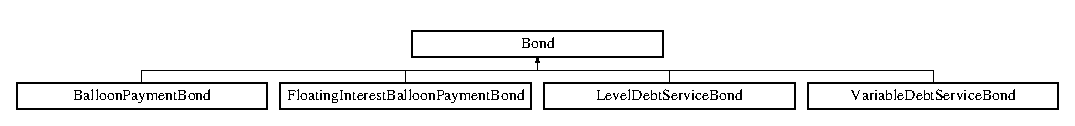
\includegraphics[height=1.244444cm]{classBond}
\end{center}
\end{figure}
\subsection*{Public Member Functions}
\begin{DoxyCompactItemize}
\item 
\mbox{\hyperlink{classBond_ac2ed54d795433c9c6a4236629553fb83}{Bond}} (const int \mbox{\hyperlink{classBond_a7f75bcafbc16676ad6dbafbf40afae4a}{id}}, const double \mbox{\hyperlink{classBond_ad98df7d28b398e620286f95ee085439b}{cost\+\_\+of\+\_\+capital}}, const int \mbox{\hyperlink{classBond_a4a227b6de2eeada118d82ab1633b1db8}{n\+\_\+payments}}, vector$<$ int $>$ \mbox{\hyperlink{classBond_ae8dd46fcbf95c993460ffe4ea1f52739}{pay\+\_\+on\+\_\+weeks}}, const int \mbox{\hyperlink{classBond_a48da24878beedd71cbaa990cea860667}{type}}, bool begin\+\_\+repayment\+\_\+at\+\_\+issuance=false)
\begin{DoxyCompactList}\small\item\em Constructs a \mbox{\hyperlink{classBond}{Bond}} object with specified attributes. This function initializes a bond and validates its cost of capital. \end{DoxyCompactList}\item 
\mbox{\hyperlink{classBond_a8758b7ef325a779eeee87eb91947ce58}{Bond}} (const int \mbox{\hyperlink{classBond_a7f75bcafbc16676ad6dbafbf40afae4a}{id}}, const double \mbox{\hyperlink{classBond_ad98df7d28b398e620286f95ee085439b}{cost\+\_\+of\+\_\+capital}}, const int \mbox{\hyperlink{classBond_a4a227b6de2eeada118d82ab1633b1db8}{n\+\_\+payments}}, vector$<$ int $>$ \mbox{\hyperlink{classBond_ae8dd46fcbf95c993460ffe4ea1f52739}{pay\+\_\+on\+\_\+weeks}}, const double \mbox{\hyperlink{classBond_a5f66785534e24caa43d9f730130a6463}{coupon\+\_\+rate}}, const int \mbox{\hyperlink{classBond_a48da24878beedd71cbaa990cea860667}{type}}, bool begin\+\_\+repayment\+\_\+at\+\_\+issuance=false)
\begin{DoxyCompactList}\small\item\em Constructs a \mbox{\hyperlink{classBond}{Bond}} object with specified attributes. This function initializes a bond with a coupon rate and validates its cost of capital. \end{DoxyCompactList}\item 
\mbox{\hyperlink{classBond_a5b809c10637a30a2b24ed01609d68711}{Bond}} ()
\begin{DoxyCompactList}\small\item\em Constructs a default \mbox{\hyperlink{classBond}{Bond}} object with uninitialized values. This function initializes a \mbox{\hyperlink{classBond}{Bond}} object with placeholder values. \end{DoxyCompactList}\item 
virtual \mbox{\hyperlink{classBond_acd301f8d3b4f29e1f797f98d3a2a0b80}{$\sim$\+Bond}} ()
\begin{DoxyCompactList}\small\item\em Destroys the \mbox{\hyperlink{classBond}{Bond}} object. This function cleans up resources used by the \mbox{\hyperlink{classBond}{Bond}} object. \end{DoxyCompactList}\item 
\mbox{\hyperlink{classBond_acaa8874ed5e81057eeb7dc55fb6b5373}{Bond}} (const \mbox{\hyperlink{classBond}{Bond}} \&)=default
\item 
virtual double \mbox{\hyperlink{classBond_a98d8ecaf4b36319674ebd220598996bc}{get\+Debt\+Service}} (int week)=0
\begin{DoxyCompactList}\small\item\em Gets the debt service for the bond. This function is intended to be overridden in derived classes and is not meant to be called directly on the base {\ttfamily \mbox{\hyperlink{classBond}{Bond}}} class. \end{DoxyCompactList}\item 
virtual double \mbox{\hyperlink{classBond_a322d4ab0c0c72824ac4df5df80f14d24}{get\+Present\+Value\+Debt\+Service}} (int week, double discount\+\_\+rate)=0
\begin{DoxyCompactList}\small\item\em Get the Present Value Debt Service object. This function is intended to be overridden in derived classes and is not meant to be called directly on the base {\ttfamily \mbox{\hyperlink{classBond}{Bond}}} class. \end{DoxyCompactList}\item 
virtual void \mbox{\hyperlink{classBond_aff7fc4e1edcf199fb592d22c765b854e}{set\+Debt\+Service}} (double updated\+\_\+allocated\+\_\+fraction\+\_\+of\+\_\+annual\+\_\+debt\+\_\+service)
\begin{DoxyCompactList}\small\item\em Sets the debt service for the bond. This function is intended to be overridden in derived classes and is not meant to be called directly on the base {\ttfamily \mbox{\hyperlink{classBond}{Bond}}} class. \end{DoxyCompactList}\item 
virtual int \mbox{\hyperlink{classBond_a8190ab6482e6a9481afca4840147527e}{get\+Water\+Source\+ID}} ()
\begin{DoxyCompactList}\small\item\em Returns the bond\textquotesingle{}s unique identifier. This function retrieves the {\ttfamily id} of the bond, which serves as its water source ID. \end{DoxyCompactList}\item 
virtual double \mbox{\hyperlink{classBond_a5997278813deb16aa5d01bbca8ecc7b2}{get\+Net\+Present\+Value\+At\+Issuance}} (double discount\+\_\+rate, int week) const =0
\item 
virtual void \mbox{\hyperlink{classBond_a726edbe3ea7047ebc7246585943763e3}{issue\+Bond}} (int week, int construction\+\_\+time, double bond\+\_\+term\+\_\+multiplier, double bond\+\_\+interest\+\_\+rate\+\_\+multiplier)
\begin{DoxyCompactList}\small\item\em Issues a bond and adjusts its parameters based on given multipliers. This function sets the repayment start date and modifies bond parameters upon issuance. \end{DoxyCompactList}\item 
virtual void \mbox{\hyperlink{classBond_aadfa02c42f31c590cee31a455bdda0b2}{set\+Realization\+Water\+Source}} (unsigned long r, vector$<$ double $>$ \&rdm\+\_\+factors)
\begin{DoxyCompactList}\small\item\em Adjusts the bond\textquotesingle{}s cost of capital based on a realization factor. This function modifies the bond\textquotesingle{}s cost of capital using a random factor. \end{DoxyCompactList}\item 
bool \mbox{\hyperlink{classBond_a6342f3dd3295771b71ac1fcc3b666a42}{is\+Issued}} () const
\begin{DoxyCompactList}\small\item\em Checks if the bond has been issued. This function returns whether the bond has been marked as issued. \end{DoxyCompactList}\item 
void \mbox{\hyperlink{classBond_a573de514b0044cec6a76bb63b098b40a}{set\+Issued}} ()
\begin{DoxyCompactList}\small\item\em Marks the bond as issued. This function sets the {\ttfamily issued} status of the bond to {\ttfamily true}. \end{DoxyCompactList}\item 
double \mbox{\hyperlink{classBond_aa3773136ec3327a88226859ea950a7b3}{get\+Cost\+Of\+Capital}} ()
\begin{DoxyCompactList}\small\item\em Returns the cost of capital required to issue the bond. This function retrieves the {\ttfamily cost\+\_\+of\+\_\+capital} of the bond. \end{DoxyCompactList}\item 
void \mbox{\hyperlink{classBond_ad4e613d485dd3f1de25c8faf21faec35}{adjust\+Cost\+Of\+Capital}} (double reduction)
\begin{DoxyCompactList}\small\item\em Adjusts the bond\textquotesingle{}s cost of capital by a specified reduction. This function decreases the bond\textquotesingle{}s {\ttfamily cost\+\_\+of\+\_\+capital} by the given reduction value. \end{DoxyCompactList}\end{DoxyCompactItemize}
\subsection*{Public Attributes}
\begin{DoxyCompactItemize}
\item 
const int \mbox{\hyperlink{classBond_a48da24878beedd71cbaa990cea860667}{type}}
\begin{DoxyCompactList}\small\item\em The type of bond. \end{DoxyCompactList}\item 
const vector$<$ int $>$ \mbox{\hyperlink{classBond_ae8dd46fcbf95c993460ffe4ea1f52739}{pay\+\_\+on\+\_\+weeks}}
\begin{DoxyCompactList}\small\item\em A vector specifying the weeks when payments are due. \end{DoxyCompactList}\item 
const int \mbox{\hyperlink{classBond_a7f75bcafbc16676ad6dbafbf40afae4a}{id}}
\begin{DoxyCompactList}\small\item\em The unique identifier of the bond. \end{DoxyCompactList}\end{DoxyCompactItemize}
\subsection*{Protected Attributes}
\begin{DoxyCompactItemize}
\item 
int \mbox{\hyperlink{classBond_a30d48d158cbbd9c7b4bfa0012c89590a}{week\+\_\+issued}}
\begin{DoxyCompactList}\small\item\em The week the bond was issued. \end{DoxyCompactList}\item 
double \mbox{\hyperlink{classBond_ad98df7d28b398e620286f95ee085439b}{cost\+\_\+of\+\_\+capital}}
\begin{DoxyCompactList}\small\item\em The cost of capital for the bond. \end{DoxyCompactList}\item 
double \mbox{\hyperlink{classBond_a5f66785534e24caa43d9f730130a6463}{coupon\+\_\+rate}}
\begin{DoxyCompactList}\small\item\em The fixed interest rate paid to bondholders each year, as a percentage of the bond\textquotesingle{}s face value. \end{DoxyCompactList}\item 
int \mbox{\hyperlink{classBond_a4a227b6de2eeada118d82ab1633b1db8}{n\+\_\+payments}}
\begin{DoxyCompactList}\small\item\em The number of payments to be made on the bond. \end{DoxyCompactList}\item 
int \mbox{\hyperlink{classBond_a8d808753f9708e841dfceca72a110737}{begin\+\_\+repayment\+\_\+after\+\_\+n\+\_\+years}} = N\+O\+N\+\_\+\+I\+N\+I\+T\+I\+A\+L\+I\+Z\+ED
\begin{DoxyCompactList}\small\item\em The number of years after issuance that the bond will start being repaid. \end{DoxyCompactList}\end{DoxyCompactItemize}


\subsection{Constructor \& Destructor Documentation}
\mbox{\Hypertarget{classBond_ac2ed54d795433c9c6a4236629553fb83}\label{classBond_ac2ed54d795433c9c6a4236629553fb83}} 
\index{Bond@{Bond}!Bond@{Bond}}
\index{Bond@{Bond}!Bond@{Bond}}
\subsubsection{\texorpdfstring{Bond()}{Bond()}\hspace{0.1cm}{\footnotesize\ttfamily [1/4]}}
{\footnotesize\ttfamily Bond\+::\+Bond (\begin{DoxyParamCaption}\item[{const int}]{id,  }\item[{const double}]{cost\+\_\+of\+\_\+capital,  }\item[{const int}]{n\+\_\+payments,  }\item[{vector$<$ int $>$}]{pay\+\_\+on\+\_\+weeks,  }\item[{const int}]{type,  }\item[{bool}]{begin\+\_\+repayment\+\_\+at\+\_\+issuance = {\ttfamily false} }\end{DoxyParamCaption})}



Constructs a \mbox{\hyperlink{classBond}{Bond}} object with specified attributes. This function initializes a bond and validates its cost of capital. 


\begin{DoxyParams}{Parameters}
{\em id} & The unique identifier for the bond. \\
\hline
{\em cost\+\_\+of\+\_\+capital} & The cost of capital associated with the bond. Must be non-\/negative. \\
\hline
{\em n\+\_\+payments} & The total number of payments for the bond. \\
\hline
{\em pay\+\_\+on\+\_\+weeks} & A vector specifying the weeks when payments are due. \\
\hline
{\em type} & The type of bond. \\
\hline
{\em begin\+\_\+repayment\+\_\+at\+\_\+issuance} & Boolean indicating whether repayment starts immediately upon issuance.\\
\hline
\end{DoxyParams}

\begin{DoxyExceptions}{Exceptions}
{\em std\+::invalid\+\_\+argument} & If {\ttfamily cost\+\_\+of\+\_\+capital} is NaN or negative. \\
\hline
\end{DoxyExceptions}
\mbox{\Hypertarget{classBond_a8758b7ef325a779eeee87eb91947ce58}\label{classBond_a8758b7ef325a779eeee87eb91947ce58}} 
\index{Bond@{Bond}!Bond@{Bond}}
\index{Bond@{Bond}!Bond@{Bond}}
\subsubsection{\texorpdfstring{Bond()}{Bond()}\hspace{0.1cm}{\footnotesize\ttfamily [2/4]}}
{\footnotesize\ttfamily Bond\+::\+Bond (\begin{DoxyParamCaption}\item[{const int}]{id,  }\item[{const double}]{cost\+\_\+of\+\_\+capital,  }\item[{const int}]{n\+\_\+payments,  }\item[{vector$<$ int $>$}]{pay\+\_\+on\+\_\+weeks,  }\item[{const double}]{coupon\+\_\+rate,  }\item[{const int}]{type,  }\item[{bool}]{begin\+\_\+repayment\+\_\+at\+\_\+issuance = {\ttfamily false} }\end{DoxyParamCaption})}



Constructs a \mbox{\hyperlink{classBond}{Bond}} object with specified attributes. This function initializes a bond with a coupon rate and validates its cost of capital. 


\begin{DoxyParams}{Parameters}
{\em id} & The unique identifier for the bond. \\
\hline
{\em cost\+\_\+of\+\_\+capital} & The cost of capital associated with the bond. Must be non-\/negative. \\
\hline
{\em n\+\_\+payments} & The total number of payments for the bond. \\
\hline
{\em pay\+\_\+on\+\_\+weeks} & A vector specifying the weeks when payments are due. \\
\hline
{\em coupon\+\_\+rate} & The fixed interest rate paid to bondholders each year associated with the bond. \\
\hline
{\em type} & The type identifier for the bond. \\
\hline
{\em begin\+\_\+repayment\+\_\+at\+\_\+issuance} & Boolean indicating whether repayment starts immediately upon issuance.\\
\hline
\end{DoxyParams}

\begin{DoxyExceptions}{Exceptions}
{\em std\+::invalid\+\_\+argument} & If {\ttfamily cost\+\_\+of\+\_\+capital} is NaN or negative. \\
\hline
\end{DoxyExceptions}
\mbox{\Hypertarget{classBond_a5b809c10637a30a2b24ed01609d68711}\label{classBond_a5b809c10637a30a2b24ed01609d68711}} 
\index{Bond@{Bond}!Bond@{Bond}}
\index{Bond@{Bond}!Bond@{Bond}}
\subsubsection{\texorpdfstring{Bond()}{Bond()}\hspace{0.1cm}{\footnotesize\ttfamily [3/4]}}
{\footnotesize\ttfamily Bond\+::\+Bond (\begin{DoxyParamCaption}{ }\end{DoxyParamCaption})}



Constructs a default \mbox{\hyperlink{classBond}{Bond}} object with uninitialized values. This function initializes a \mbox{\hyperlink{classBond}{Bond}} object with placeholder values. 

\mbox{\Hypertarget{classBond_acd301f8d3b4f29e1f797f98d3a2a0b80}\label{classBond_acd301f8d3b4f29e1f797f98d3a2a0b80}} 
\index{Bond@{Bond}!````~Bond@{$\sim$\+Bond}}
\index{````~Bond@{$\sim$\+Bond}!Bond@{Bond}}
\subsubsection{\texorpdfstring{$\sim$\+Bond()}{~Bond()}}
{\footnotesize\ttfamily virtual Bond\+::$\sim$\+Bond (\begin{DoxyParamCaption}{ }\end{DoxyParamCaption})\hspace{0.3cm}{\ttfamily [virtual]}}



Destroys the \mbox{\hyperlink{classBond}{Bond}} object. This function cleans up resources used by the \mbox{\hyperlink{classBond}{Bond}} object. 

\mbox{\Hypertarget{classBond_acaa8874ed5e81057eeb7dc55fb6b5373}\label{classBond_acaa8874ed5e81057eeb7dc55fb6b5373}} 
\index{Bond@{Bond}!Bond@{Bond}}
\index{Bond@{Bond}!Bond@{Bond}}
\subsubsection{\texorpdfstring{Bond()}{Bond()}\hspace{0.1cm}{\footnotesize\ttfamily [4/4]}}
{\footnotesize\ttfamily Bond\+::\+Bond (\begin{DoxyParamCaption}\item[{const \mbox{\hyperlink{classBond}{Bond}} \&}]{ }\end{DoxyParamCaption})\hspace{0.3cm}{\ttfamily [default]}}



\subsection{Member Function Documentation}
\mbox{\Hypertarget{classBond_ad4e613d485dd3f1de25c8faf21faec35}\label{classBond_ad4e613d485dd3f1de25c8faf21faec35}} 
\index{Bond@{Bond}!adjust\+Cost\+Of\+Capital@{adjust\+Cost\+Of\+Capital}}
\index{adjust\+Cost\+Of\+Capital@{adjust\+Cost\+Of\+Capital}!Bond@{Bond}}
\subsubsection{\texorpdfstring{adjust\+Cost\+Of\+Capital()}{adjustCostOfCapital()}}
{\footnotesize\ttfamily void Bond\+::adjust\+Cost\+Of\+Capital (\begin{DoxyParamCaption}\item[{double}]{reduction }\end{DoxyParamCaption})}



Adjusts the bond\textquotesingle{}s cost of capital by a specified reduction. This function decreases the bond\textquotesingle{}s {\ttfamily cost\+\_\+of\+\_\+capital} by the given reduction value. 


\begin{DoxyParams}{Parameters}
{\em reduction} & The amount by which to reduce the bond\textquotesingle{}s {\ttfamily cost\+\_\+of\+\_\+capital}.\\
\hline
\end{DoxyParams}
\begin{DoxyReturn}{Returns}
None
\end{DoxyReturn}

\begin{DoxyExceptions}{Exceptions}
{\em std\+::logic\+\_\+error} & If the adjusted {\ttfamily cost\+\_\+of\+\_\+capital} becomes negative. \\
\hline
\end{DoxyExceptions}
\mbox{\Hypertarget{classBond_aa3773136ec3327a88226859ea950a7b3}\label{classBond_aa3773136ec3327a88226859ea950a7b3}} 
\index{Bond@{Bond}!get\+Cost\+Of\+Capital@{get\+Cost\+Of\+Capital}}
\index{get\+Cost\+Of\+Capital@{get\+Cost\+Of\+Capital}!Bond@{Bond}}
\subsubsection{\texorpdfstring{get\+Cost\+Of\+Capital()}{getCostOfCapital()}}
{\footnotesize\ttfamily double Bond\+::get\+Cost\+Of\+Capital (\begin{DoxyParamCaption}{ }\end{DoxyParamCaption})}



Returns the cost of capital required to issue the bond. This function retrieves the {\ttfamily cost\+\_\+of\+\_\+capital} of the bond. 


\begin{DoxyParams}{Parameters}
{\em None} & \\
\hline
\end{DoxyParams}
\begin{DoxyReturn}{Returns}
double The cost of capital ({\ttfamily cost\+\_\+of\+\_\+capital}) of the bond. 
\end{DoxyReturn}
\mbox{\Hypertarget{classBond_a98d8ecaf4b36319674ebd220598996bc}\label{classBond_a98d8ecaf4b36319674ebd220598996bc}} 
\index{Bond@{Bond}!get\+Debt\+Service@{get\+Debt\+Service}}
\index{get\+Debt\+Service@{get\+Debt\+Service}!Bond@{Bond}}
\subsubsection{\texorpdfstring{get\+Debt\+Service()}{getDebtService()}}
{\footnotesize\ttfamily virtual double Bond\+::get\+Debt\+Service (\begin{DoxyParamCaption}\item[{int}]{week }\end{DoxyParamCaption})\hspace{0.3cm}{\ttfamily [pure virtual]}}



Gets the debt service for the bond. This function is intended to be overridden in derived classes and is not meant to be called directly on the base {\ttfamily \mbox{\hyperlink{classBond}{Bond}}} class. 


\begin{DoxyParams}{Parameters}
{\em week} & The week for which to calculate total remaining value of the debt service (accounting for inflation). \\
\hline
\end{DoxyParams}
\begin{DoxyReturn}{Returns}
double The debt service for the bond. 
\end{DoxyReturn}


Implemented in \mbox{\hyperlink{classVariableDebtServiceBond_a575a9a41df38e005ba0a1cff3eb2b921}{Variable\+Debt\+Service\+Bond}}, \mbox{\hyperlink{classBalloonPaymentBond_a8648a2ae688f90a3b2e6689711c22b9d}{Balloon\+Payment\+Bond}}, \mbox{\hyperlink{classFloatingInterestBalloonPaymentBond_a0009a0b12e0ebeb15952561513ddc901}{Floating\+Interest\+Balloon\+Payment\+Bond}}, and \mbox{\hyperlink{classLevelDebtServiceBond_adcb3bd3c34b0cbb7b013f387ddd8b7f5}{Level\+Debt\+Service\+Bond}}.

\mbox{\Hypertarget{classBond_a5997278813deb16aa5d01bbca8ecc7b2}\label{classBond_a5997278813deb16aa5d01bbca8ecc7b2}} 
\index{Bond@{Bond}!get\+Net\+Present\+Value\+At\+Issuance@{get\+Net\+Present\+Value\+At\+Issuance}}
\index{get\+Net\+Present\+Value\+At\+Issuance@{get\+Net\+Present\+Value\+At\+Issuance}!Bond@{Bond}}
\subsubsection{\texorpdfstring{get\+Net\+Present\+Value\+At\+Issuance()}{getNetPresentValueAtIssuance()}}
{\footnotesize\ttfamily virtual double Bond\+::get\+Net\+Present\+Value\+At\+Issuance (\begin{DoxyParamCaption}\item[{double}]{discount\+\_\+rate,  }\item[{int}]{week }\end{DoxyParamCaption}) const\hspace{0.3cm}{\ttfamily [pure virtual]}}



Implemented in \mbox{\hyperlink{classVariableDebtServiceBond_a8cc7ee442d788b91b8c00e6bed07644d}{Variable\+Debt\+Service\+Bond}}, \mbox{\hyperlink{classBalloonPaymentBond_abbfaae70e003f057ec842d3889138345}{Balloon\+Payment\+Bond}}, \mbox{\hyperlink{classFloatingInterestBalloonPaymentBond_a90205e26e09eef1227f8c0671ca4fce2}{Floating\+Interest\+Balloon\+Payment\+Bond}}, and \mbox{\hyperlink{classLevelDebtServiceBond_a0f5820c3e76b8b908dbe153a8291d96a}{Level\+Debt\+Service\+Bond}}.

\mbox{\Hypertarget{classBond_a322d4ab0c0c72824ac4df5df80f14d24}\label{classBond_a322d4ab0c0c72824ac4df5df80f14d24}} 
\index{Bond@{Bond}!get\+Present\+Value\+Debt\+Service@{get\+Present\+Value\+Debt\+Service}}
\index{get\+Present\+Value\+Debt\+Service@{get\+Present\+Value\+Debt\+Service}!Bond@{Bond}}
\subsubsection{\texorpdfstring{get\+Present\+Value\+Debt\+Service()}{getPresentValueDebtService()}}
{\footnotesize\ttfamily virtual double Bond\+::get\+Present\+Value\+Debt\+Service (\begin{DoxyParamCaption}\item[{int}]{week,  }\item[{double}]{discount\+\_\+rate }\end{DoxyParamCaption})\hspace{0.3cm}{\ttfamily [pure virtual]}}



Get the Present Value Debt Service object. This function is intended to be overridden in derived classes and is not meant to be called directly on the base {\ttfamily \mbox{\hyperlink{classBond}{Bond}}} class. 


\begin{DoxyParams}{Parameters}
{\em week} & The week for which to calculate the present value of debt service. \\
\hline
{\em discount\+\_\+rate} & The discount rate to use in the calculation. \\
\hline
\end{DoxyParams}
\begin{DoxyReturn}{Returns}
double The present value of the debt service. 
\end{DoxyReturn}


Implemented in \mbox{\hyperlink{classVariableDebtServiceBond_aa5ad4fcc7c65154105388b332ae98198}{Variable\+Debt\+Service\+Bond}}, \mbox{\hyperlink{classBalloonPaymentBond_ae038863f7a3408c2c8cd503d8e789f2d}{Balloon\+Payment\+Bond}}, \mbox{\hyperlink{classFloatingInterestBalloonPaymentBond_a91b2fef92f90049a3ba13bcd27c0eff2}{Floating\+Interest\+Balloon\+Payment\+Bond}}, and \mbox{\hyperlink{classLevelDebtServiceBond_a37801ecfc13ae1b6e05b4330398a7582}{Level\+Debt\+Service\+Bond}}.

\mbox{\Hypertarget{classBond_a8190ab6482e6a9481afca4840147527e}\label{classBond_a8190ab6482e6a9481afca4840147527e}} 
\index{Bond@{Bond}!get\+Water\+Source\+ID@{get\+Water\+Source\+ID}}
\index{get\+Water\+Source\+ID@{get\+Water\+Source\+ID}!Bond@{Bond}}
\subsubsection{\texorpdfstring{get\+Water\+Source\+I\+D()}{getWaterSourceID()}}
{\footnotesize\ttfamily virtual int Bond\+::get\+Water\+Source\+ID (\begin{DoxyParamCaption}{ }\end{DoxyParamCaption})\hspace{0.3cm}{\ttfamily [virtual]}}



Returns the bond\textquotesingle{}s unique identifier. This function retrieves the {\ttfamily id} of the bond, which serves as its water source ID. 


\begin{DoxyParams}{Parameters}
{\em None} & \\
\hline
\end{DoxyParams}
\begin{DoxyReturn}{Returns}
int The unique identifier ({\ttfamily id}) of the bond. 
\end{DoxyReturn}


Reimplemented in \mbox{\hyperlink{classVariableDebtServiceBond_a3edee29f26e8ac74f9767770c6a951c9}{Variable\+Debt\+Service\+Bond}}.

\mbox{\Hypertarget{classBond_a6342f3dd3295771b71ac1fcc3b666a42}\label{classBond_a6342f3dd3295771b71ac1fcc3b666a42}} 
\index{Bond@{Bond}!is\+Issued@{is\+Issued}}
\index{is\+Issued@{is\+Issued}!Bond@{Bond}}
\subsubsection{\texorpdfstring{is\+Issued()}{isIssued()}}
{\footnotesize\ttfamily bool Bond\+::is\+Issued (\begin{DoxyParamCaption}{ }\end{DoxyParamCaption}) const}



Checks if the bond has been issued. This function returns whether the bond has been marked as issued. 


\begin{DoxyParams}{Parameters}
{\em None} & \\
\hline
\end{DoxyParams}
\begin{DoxyReturn}{Returns}
bool {\ttfamily true} if the bond has been issued; {\ttfamily false} otherwise. 
\end{DoxyReturn}
\mbox{\Hypertarget{classBond_a726edbe3ea7047ebc7246585943763e3}\label{classBond_a726edbe3ea7047ebc7246585943763e3}} 
\index{Bond@{Bond}!issue\+Bond@{issue\+Bond}}
\index{issue\+Bond@{issue\+Bond}!Bond@{Bond}}
\subsubsection{\texorpdfstring{issue\+Bond()}{issueBond()}}
{\footnotesize\ttfamily virtual void Bond\+::issue\+Bond (\begin{DoxyParamCaption}\item[{int}]{week,  }\item[{int}]{construction\+\_\+time,  }\item[{double}]{bond\+\_\+term\+\_\+multiplier,  }\item[{double}]{bond\+\_\+interest\+\_\+rate\+\_\+multiplier }\end{DoxyParamCaption})\hspace{0.3cm}{\ttfamily [virtual]}}



Issues a bond and adjusts its parameters based on given multipliers. This function sets the repayment start date and modifies bond parameters upon issuance. 


\begin{DoxyParams}{Parameters}
{\em week} & The week when the bond is issued. \\
\hline
{\em construction\+\_\+time} & The duration of construction in weeks, used to calculate the repayment start date. \\
\hline
{\em bond\+\_\+term\+\_\+multiplier} & A multiplier to adjust the total number of payments. \\
\hline
{\em bond\+\_\+interest\+\_\+rate\+\_\+multiplier} & A multiplier to adjust the bond\textquotesingle{}s coupon rate.\\
\hline
\end{DoxyParams}
\begin{DoxyReturn}{Returns}
None
\end{DoxyReturn}
\begin{DoxySeeAlso}{See also}
\mbox{\hyperlink{classBond_a573de514b0044cec6a76bb63b098b40a}{Bond\+::set\+Issued}} 
\end{DoxySeeAlso}


Reimplemented in \mbox{\hyperlink{classVariableDebtServiceBond_a7d91921482f01d9bb37dba6e6d085771}{Variable\+Debt\+Service\+Bond}}, \mbox{\hyperlink{classBalloonPaymentBond_af22552acd74b08dbb1d308cc5e45344c}{Balloon\+Payment\+Bond}}, \mbox{\hyperlink{classFloatingInterestBalloonPaymentBond_a4cf110f320c92f5eca9aed952e0b527a}{Floating\+Interest\+Balloon\+Payment\+Bond}}, and \mbox{\hyperlink{classLevelDebtServiceBond_a51a54a1a25be105b168bf86489aee417}{Level\+Debt\+Service\+Bond}}.

\mbox{\Hypertarget{classBond_aff7fc4e1edcf199fb592d22c765b854e}\label{classBond_aff7fc4e1edcf199fb592d22c765b854e}} 
\index{Bond@{Bond}!set\+Debt\+Service@{set\+Debt\+Service}}
\index{set\+Debt\+Service@{set\+Debt\+Service}!Bond@{Bond}}
\subsubsection{\texorpdfstring{set\+Debt\+Service()}{setDebtService()}}
{\footnotesize\ttfamily virtual void Bond\+::set\+Debt\+Service (\begin{DoxyParamCaption}\item[{double}]{updated\+\_\+allocated\+\_\+fraction\+\_\+of\+\_\+annual\+\_\+debt\+\_\+service }\end{DoxyParamCaption})\hspace{0.3cm}{\ttfamily [virtual]}}



Sets the debt service for the bond. This function is intended to be overridden in derived classes and is not meant to be called directly on the base {\ttfamily \mbox{\hyperlink{classBond}{Bond}}} class. 


\begin{DoxyParams}{Parameters}
{\em updated\+\_\+allocated\+\_\+fraction\+\_\+of\+\_\+annual\+\_\+debt\+\_\+service} & The updated fraction of the annual debt service allocation.\\
\hline
\end{DoxyParams}
\begin{DoxyReturn}{Returns}
None
\end{DoxyReturn}

\begin{DoxyExceptions}{Exceptions}
{\em std\+::logic\+\_\+error} & Always throws an exception when called on the base {\ttfamily \mbox{\hyperlink{classBond}{Bond}}} class. \\
\hline
\end{DoxyExceptions}


Reimplemented in \mbox{\hyperlink{classVariableDebtServiceBond_a692563150053b280f6e1ef23fd47c117}{Variable\+Debt\+Service\+Bond}}.

\mbox{\Hypertarget{classBond_a573de514b0044cec6a76bb63b098b40a}\label{classBond_a573de514b0044cec6a76bb63b098b40a}} 
\index{Bond@{Bond}!set\+Issued@{set\+Issued}}
\index{set\+Issued@{set\+Issued}!Bond@{Bond}}
\subsubsection{\texorpdfstring{set\+Issued()}{setIssued()}}
{\footnotesize\ttfamily void Bond\+::set\+Issued (\begin{DoxyParamCaption}{ }\end{DoxyParamCaption})}



Marks the bond as issued. This function sets the {\ttfamily issued} status of the bond to {\ttfamily true}. 


\begin{DoxyParams}{Parameters}
{\em None} & \\
\hline
\end{DoxyParams}
\begin{DoxyReturn}{Returns}
None 
\end{DoxyReturn}
\mbox{\Hypertarget{classBond_aadfa02c42f31c590cee31a455bdda0b2}\label{classBond_aadfa02c42f31c590cee31a455bdda0b2}} 
\index{Bond@{Bond}!set\+Realization\+Water\+Source@{set\+Realization\+Water\+Source}}
\index{set\+Realization\+Water\+Source@{set\+Realization\+Water\+Source}!Bond@{Bond}}
\subsubsection{\texorpdfstring{set\+Realization\+Water\+Source()}{setRealizationWaterSource()}}
{\footnotesize\ttfamily virtual void Bond\+::set\+Realization\+Water\+Source (\begin{DoxyParamCaption}\item[{unsigned long}]{r,  }\item[{vector$<$ double $>$ \&}]{rdm\+\_\+factors }\end{DoxyParamCaption})\hspace{0.3cm}{\ttfamily [virtual]}}



Adjusts the bond\textquotesingle{}s cost of capital based on a realization factor. This function modifies the bond\textquotesingle{}s cost of capital using a random factor. 


\begin{DoxyParams}{Parameters}
{\em r} & An unsigned long integer representing the realization identifier (not used in the function logic). \\
\hline
{\em rdm\+\_\+factors} & A vector of random factors used to adjust the bond\textquotesingle{}s cost of capital. The first element is used.\\
\hline
\end{DoxyParams}
\begin{DoxyReturn}{Returns}
None
\end{DoxyReturn}

\begin{DoxyExceptions}{Exceptions}
{\em std\+::out\+\_\+of\+\_\+range} & If {\ttfamily rdm\+\_\+factors} is empty or does not contain at least one element.\\
\hline
\end{DoxyExceptions}
\begin{DoxySeeAlso}{See also}
\mbox{\hyperlink{classBond_a726edbe3ea7047ebc7246585943763e3}{Bond\+::issue\+Bond}} 
\end{DoxySeeAlso}


\subsection{Member Data Documentation}
\mbox{\Hypertarget{classBond_a8d808753f9708e841dfceca72a110737}\label{classBond_a8d808753f9708e841dfceca72a110737}} 
\index{Bond@{Bond}!begin\+\_\+repayment\+\_\+after\+\_\+n\+\_\+years@{begin\+\_\+repayment\+\_\+after\+\_\+n\+\_\+years}}
\index{begin\+\_\+repayment\+\_\+after\+\_\+n\+\_\+years@{begin\+\_\+repayment\+\_\+after\+\_\+n\+\_\+years}!Bond@{Bond}}
\subsubsection{\texorpdfstring{begin\+\_\+repayment\+\_\+after\+\_\+n\+\_\+years}{begin\_repayment\_after\_n\_years}}
{\footnotesize\ttfamily int Bond\+::begin\+\_\+repayment\+\_\+after\+\_\+n\+\_\+years = N\+O\+N\+\_\+\+I\+N\+I\+T\+I\+A\+L\+I\+Z\+ED\hspace{0.3cm}{\ttfamily [protected]}}



The number of years after issuance that the bond will start being repaid. 

\mbox{\Hypertarget{classBond_ad98df7d28b398e620286f95ee085439b}\label{classBond_ad98df7d28b398e620286f95ee085439b}} 
\index{Bond@{Bond}!cost\+\_\+of\+\_\+capital@{cost\+\_\+of\+\_\+capital}}
\index{cost\+\_\+of\+\_\+capital@{cost\+\_\+of\+\_\+capital}!Bond@{Bond}}
\subsubsection{\texorpdfstring{cost\+\_\+of\+\_\+capital}{cost\_of\_capital}}
{\footnotesize\ttfamily double Bond\+::cost\+\_\+of\+\_\+capital\hspace{0.3cm}{\ttfamily [protected]}}



The cost of capital for the bond. 

\mbox{\Hypertarget{classBond_a5f66785534e24caa43d9f730130a6463}\label{classBond_a5f66785534e24caa43d9f730130a6463}} 
\index{Bond@{Bond}!coupon\+\_\+rate@{coupon\+\_\+rate}}
\index{coupon\+\_\+rate@{coupon\+\_\+rate}!Bond@{Bond}}
\subsubsection{\texorpdfstring{coupon\+\_\+rate}{coupon\_rate}}
{\footnotesize\ttfamily double Bond\+::coupon\+\_\+rate\hspace{0.3cm}{\ttfamily [protected]}}



The fixed interest rate paid to bondholders each year, as a percentage of the bond\textquotesingle{}s face value. 

\mbox{\Hypertarget{classBond_a7f75bcafbc16676ad6dbafbf40afae4a}\label{classBond_a7f75bcafbc16676ad6dbafbf40afae4a}} 
\index{Bond@{Bond}!id@{id}}
\index{id@{id}!Bond@{Bond}}
\subsubsection{\texorpdfstring{id}{id}}
{\footnotesize\ttfamily const int Bond\+::id}



The unique identifier of the bond. 

\mbox{\Hypertarget{classBond_a4a227b6de2eeada118d82ab1633b1db8}\label{classBond_a4a227b6de2eeada118d82ab1633b1db8}} 
\index{Bond@{Bond}!n\+\_\+payments@{n\+\_\+payments}}
\index{n\+\_\+payments@{n\+\_\+payments}!Bond@{Bond}}
\subsubsection{\texorpdfstring{n\+\_\+payments}{n\_payments}}
{\footnotesize\ttfamily int Bond\+::n\+\_\+payments\hspace{0.3cm}{\ttfamily [protected]}}



The number of payments to be made on the bond. 

\mbox{\Hypertarget{classBond_ae8dd46fcbf95c993460ffe4ea1f52739}\label{classBond_ae8dd46fcbf95c993460ffe4ea1f52739}} 
\index{Bond@{Bond}!pay\+\_\+on\+\_\+weeks@{pay\+\_\+on\+\_\+weeks}}
\index{pay\+\_\+on\+\_\+weeks@{pay\+\_\+on\+\_\+weeks}!Bond@{Bond}}
\subsubsection{\texorpdfstring{pay\+\_\+on\+\_\+weeks}{pay\_on\_weeks}}
{\footnotesize\ttfamily const vector$<$int$>$ Bond\+::pay\+\_\+on\+\_\+weeks}



A vector specifying the weeks when payments are due. 

\mbox{\Hypertarget{classBond_a48da24878beedd71cbaa990cea860667}\label{classBond_a48da24878beedd71cbaa990cea860667}} 
\index{Bond@{Bond}!type@{type}}
\index{type@{type}!Bond@{Bond}}
\subsubsection{\texorpdfstring{type}{type}}
{\footnotesize\ttfamily const int Bond\+::type}



The type of bond. 

\mbox{\Hypertarget{classBond_a30d48d158cbbd9c7b4bfa0012c89590a}\label{classBond_a30d48d158cbbd9c7b4bfa0012c89590a}} 
\index{Bond@{Bond}!week\+\_\+issued@{week\+\_\+issued}}
\index{week\+\_\+issued@{week\+\_\+issued}!Bond@{Bond}}
\subsubsection{\texorpdfstring{week\+\_\+issued}{week\_issued}}
{\footnotesize\ttfamily int Bond\+::week\+\_\+issued\hspace{0.3cm}{\ttfamily [protected]}}



The week the bond was issued. 



The documentation for this class was generated from the following file\+:\begin{DoxyCompactItemize}
\item 
/home/fs02/pmr82\+\_\+0001/lbl59/\+Water\+Paths-\/doc/src/\+System\+Components/\+Bonds/\+Base/\mbox{\hyperlink{Bond_8h}{Bond.\+h}}\end{DoxyCompactItemize}

\hypertarget{structby__xreal}{}\section{by\+\_\+xreal Struct Reference}
\label{structby__xreal}\index{by\+\_\+xreal@{by\+\_\+xreal}}


{\ttfamily \#include $<$Problem.\+h$>$}

\subsection*{Public Member Functions}
\begin{DoxyCompactItemize}
\item 
bool \mbox{\hyperlink{structby__xreal_a89543fd1eb21d028c20e4cd01a239b71_a89543fd1eb21d028c20e4cd01a239b71}{operator()}} (const \mbox{\hyperlink{structinfraRank}{infra\+Rank}} \&ir1, const \mbox{\hyperlink{structinfraRank}{infra\+Rank}} \&ir2)
\end{DoxyCompactItemize}


\subsection{Member Function Documentation}
\mbox{\Hypertarget{structby__xreal_a89543fd1eb21d028c20e4cd01a239b71_a89543fd1eb21d028c20e4cd01a239b71}\label{structby__xreal_a89543fd1eb21d028c20e4cd01a239b71_a89543fd1eb21d028c20e4cd01a239b71}} 
\index{by\+\_\+xreal@{by\+\_\+xreal}!operator()@{operator()}}
\index{operator()@{operator()}!by\+\_\+xreal@{by\+\_\+xreal}}
\subsubsection{\texorpdfstring{operator()()}{operator()()}}
{\footnotesize\ttfamily bool by\+\_\+xreal\+::operator() (\begin{DoxyParamCaption}\item[{const \mbox{\hyperlink{structinfraRank}{infra\+Rank}} \&}]{ir1,  }\item[{const \mbox{\hyperlink{structinfraRank}{infra\+Rank}} \&}]{ir2 }\end{DoxyParamCaption})\hspace{0.3cm}{\ttfamily [inline]}}



The documentation for this struct was generated from the following file\+:\begin{DoxyCompactItemize}
\item 
src/\+Problem/\+Base/\mbox{\hyperlink{Problem_8h}{Problem.\+h}}\end{DoxyCompactItemize}

\hypertarget{classCatchment}{}\section{Catchment Class Reference}
\label{classCatchment}\index{Catchment@{Catchment}}


This class defines a catchment object.  




{\ttfamily \#include $<$Catchment.\+h$>$}

Inheritance diagram for Catchment\+:\begin{figure}[H]
\begin{center}
\leavevmode
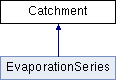
\includegraphics[height=2.000000cm]{classCatchment}
\end{center}
\end{figure}
\subsection*{Public Member Functions}
\begin{DoxyCompactItemize}
\item 
\mbox{\hyperlink{classCatchment_aafdee6ee868a8892314672abb119e60f}{Catchment}} (vector$<$ vector$<$ double $>$$>$ $\ast$\mbox{\hyperlink{classCatchment_a579ccda86831f286c19c76354e7125c3}{streamflows\+\_\+all}}, int \mbox{\hyperlink{classCatchment_a2d4994220f63b876348b4ce4892bc6d3}{series\+\_\+length}})
\begin{DoxyCompactList}\small\item\em Constructor for a new \mbox{\hyperlink{classCatchment}{Catchment}} object. \end{DoxyCompactList}\item 
\mbox{\hyperlink{classCatchment_ae311c4b2d857a8b5abc01f5317b04df2}{Catchment}} (const \mbox{\hyperlink{classCatchment}{Catchment}} \&catchment)
\begin{DoxyCompactList}\small\item\em Copy constructor for a \mbox{\hyperlink{classCatchment}{Catchment}} object. This constructor does not copy the parent pointer. Set parent to false to distinguish between a parent \mbox{\hyperlink{classCatchment}{Catchment}} and those created as copies. Initializes a new instance of \mbox{\hyperlink{classCatchment}{Catchment}} with data copied from the original \mbox{\hyperlink{classCatchment}{Catchment}} object. \end{DoxyCompactList}\item 
virtual \mbox{\hyperlink{classCatchment_ad12bc6d64d4bd5133ac1086a52e240b3}{$\sim$\+Catchment}} ()
\begin{DoxyCompactList}\small\item\em Destructor for a \mbox{\hyperlink{classCatchment}{Catchment}} object. \end{DoxyCompactList}\item 
\mbox{\hyperlink{classCatchment}{Catchment}} \& \mbox{\hyperlink{classCatchment_a5abab52eab9c05164f76e46954833989}{operator=}} (const \mbox{\hyperlink{classCatchment}{Catchment}} \&catchment)
\begin{DoxyCompactList}\small\item\em Copy assignment operator. \end{DoxyCompactList}\item 
double \mbox{\hyperlink{classCatchment_af4e8206ffab5c901e5e4cdd6136f73a1}{get\+Streamflow}} (int week)
\begin{DoxyCompactList}\small\item\em Gets streamflow for a given week A\+F\+T\+ER the first delta\+\_\+week weeks used to calculate the R\+O\+Fs. This function assures that the number of past inflows used for R\+OF calculations are reserved in the beginning of the time series for R\+OF calculations. \end{DoxyCompactList}\item 
virtual void \mbox{\hyperlink{classCatchment_ad76654af47dcd69bcb795c1c152409cc}{set\+Realization}} (unsigned long r, vector$<$ double $>$ \&rdm\+\_\+factors)
\begin{DoxyCompactList}\small\item\em Sets the 1D vector time series corresponding to realization index and eliminate reference to the full 2D comprehensive streamflow data set. \end{DoxyCompactList}\end{DoxyCompactItemize}
\subsection*{Protected Attributes}
\begin{DoxyCompactItemize}
\item 
vector$<$ vector$<$ double $>$ $>$ $\ast$ \mbox{\hyperlink{classCatchment_a579ccda86831f286c19c76354e7125c3}{streamflows\+\_\+all}}
\begin{DoxyCompactList}\small\item\em A pointer to a 2D vector containing all combined historical and synthetic streamflow realizations. \end{DoxyCompactList}\item 
vector$<$ double $>$ \mbox{\hyperlink{classCatchment_aaf04c295ecd6b666fa1439d3d5bc072a}{streamflows\+\_\+realization}}
\begin{DoxyCompactList}\small\item\em A 1D vector containing the streamflows for a specific realization for the catchment. \end{DoxyCompactList}\item 
int \mbox{\hyperlink{classCatchment_a2d4994220f63b876348b4ce4892bc6d3}{series\+\_\+length}}
\begin{DoxyCompactList}\small\item\em An integer representing the length of the streamflow time series. It should be longer than W\+E\+E\+K\+S\+\_\+\+I\+N\+\_\+\+Y\+E\+AR $\ast$ N\+U\+M\+B\+E\+R\+\_\+\+R\+E\+A\+L\+I\+Z\+A\+T\+I\+O\+N\+S\+\_\+\+R\+OF. \end{DoxyCompactList}\item 
bool \mbox{\hyperlink{classCatchment_a472ff6892f90d94b8c4dba53c462dedf}{parent}} = true
\begin{DoxyCompactList}\small\item\em A boolean indicating whether this catchment is a parent catchment or not. Parent catchments are catchments (I\+N\+S\+E\+RT D\+E\+S\+C\+R\+I\+P\+T\+I\+ON H\+E\+RE). \end{DoxyCompactList}\item 
int \mbox{\hyperlink{classCatchment_a20548a9d03f0d39f297cb15b3c0433ad}{delta\+\_\+week}}
\begin{DoxyCompactList}\small\item\em An integer indicating the number of weeks to skip in the beginning of the time series to identify the correct week for the start of a given realization. This is the number of weeks of historical data used to calculate the R\+O\+Fs. Should take on the value of W\+E\+E\+K\+S\+\_\+\+I\+N\+\_\+\+Y\+E\+AR $\ast$ N\+U\+M\+B\+E\+R\+\_\+\+R\+E\+A\+L\+I\+Z\+A\+T\+I\+O\+N\+S\+\_\+\+R\+OF. \end{DoxyCompactList}\end{DoxyCompactItemize}


\subsection{Detailed Description}
This class defines a catchment object. 

Created by bernardo on 1/13/17. 

\subsection{Constructor \& Destructor Documentation}
\mbox{\Hypertarget{classCatchment_aafdee6ee868a8892314672abb119e60f}\label{classCatchment_aafdee6ee868a8892314672abb119e60f}} 
\index{Catchment@{Catchment}!Catchment@{Catchment}}
\index{Catchment@{Catchment}!Catchment@{Catchment}}
\subsubsection{\texorpdfstring{Catchment()}{Catchment()}\hspace{0.1cm}{\footnotesize\ttfamily [1/2]}}
{\footnotesize\ttfamily Catchment\+::\+Catchment (\begin{DoxyParamCaption}\item[{vector$<$ vector$<$ double $>$$>$ $\ast$}]{streamflows\+\_\+all,  }\item[{int}]{series\+\_\+length }\end{DoxyParamCaption})}



Constructor for a new \mbox{\hyperlink{classCatchment}{Catchment}} object. 


\begin{DoxyParams}{Parameters}
{\em streamflows\+\_\+all} & A 2D vector containing all combined historical and synthetic streamflow realizations. \\
\hline
{\em series\+\_\+length} & An integer representing the length of the streamflow time series. \\
\hline
\end{DoxyParams}
\mbox{\Hypertarget{classCatchment_ae311c4b2d857a8b5abc01f5317b04df2}\label{classCatchment_ae311c4b2d857a8b5abc01f5317b04df2}} 
\index{Catchment@{Catchment}!Catchment@{Catchment}}
\index{Catchment@{Catchment}!Catchment@{Catchment}}
\subsubsection{\texorpdfstring{Catchment()}{Catchment()}\hspace{0.1cm}{\footnotesize\ttfamily [2/2]}}
{\footnotesize\ttfamily Catchment\+::\+Catchment (\begin{DoxyParamCaption}\item[{const \mbox{\hyperlink{classCatchment}{Catchment}} \&}]{catchment }\end{DoxyParamCaption})}



Copy constructor for a \mbox{\hyperlink{classCatchment}{Catchment}} object. This constructor does not copy the parent pointer. Set parent to false to distinguish between a parent \mbox{\hyperlink{classCatchment}{Catchment}} and those created as copies. Initializes a new instance of \mbox{\hyperlink{classCatchment}{Catchment}} with data copied from the original \mbox{\hyperlink{classCatchment}{Catchment}} object. 


\begin{DoxyParams}{Parameters}
{\em catchment} & A \mbox{\hyperlink{classCatchment}{Catchment}} object. \\
\hline
\end{DoxyParams}
\mbox{\Hypertarget{classCatchment_ad12bc6d64d4bd5133ac1086a52e240b3}\label{classCatchment_ad12bc6d64d4bd5133ac1086a52e240b3}} 
\index{Catchment@{Catchment}!````~Catchment@{$\sim$\+Catchment}}
\index{````~Catchment@{$\sim$\+Catchment}!Catchment@{Catchment}}
\subsubsection{\texorpdfstring{$\sim$\+Catchment()}{~Catchment()}}
{\footnotesize\ttfamily virtual Catchment\+::$\sim$\+Catchment (\begin{DoxyParamCaption}{ }\end{DoxyParamCaption})\hspace{0.3cm}{\ttfamily [virtual]}}



Destructor for a \mbox{\hyperlink{classCatchment}{Catchment}} object. 



\subsection{Member Function Documentation}
\mbox{\Hypertarget{classCatchment_af4e8206ffab5c901e5e4cdd6136f73a1}\label{classCatchment_af4e8206ffab5c901e5e4cdd6136f73a1}} 
\index{Catchment@{Catchment}!get\+Streamflow@{get\+Streamflow}}
\index{get\+Streamflow@{get\+Streamflow}!Catchment@{Catchment}}
\subsubsection{\texorpdfstring{get\+Streamflow()}{getStreamflow()}}
{\footnotesize\ttfamily double Catchment\+::get\+Streamflow (\begin{DoxyParamCaption}\item[{int}]{week }\end{DoxyParamCaption})}



Gets streamflow for a given week A\+F\+T\+ER the first delta\+\_\+week weeks used to calculate the R\+O\+Fs. This function assures that the number of past inflows used for R\+OF calculations are reserved in the beginning of the time series for R\+OF calculations. 


\begin{DoxyParams}{Parameters}
{\em week} & An integer representing the week of the entire streamflow time series. \\
\hline
\end{DoxyParams}
\begin{DoxyReturn}{Returns}
A double representing the streamflow for the given week. 
\end{DoxyReturn}
\mbox{\Hypertarget{classCatchment_a5abab52eab9c05164f76e46954833989}\label{classCatchment_a5abab52eab9c05164f76e46954833989}} 
\index{Catchment@{Catchment}!operator=@{operator=}}
\index{operator=@{operator=}!Catchment@{Catchment}}
\subsubsection{\texorpdfstring{operator=()}{operator=()}}
{\footnotesize\ttfamily \mbox{\hyperlink{classCatchment}{Catchment}}\& Catchment\+::operator= (\begin{DoxyParamCaption}\item[{const \mbox{\hyperlink{classCatchment}{Catchment}} \&}]{catchment }\end{DoxyParamCaption})}



Copy assignment operator. 


\begin{DoxyParams}{Parameters}
{\em catchment} & \\
\hline
\end{DoxyParams}
\mbox{\Hypertarget{classCatchment_ad76654af47dcd69bcb795c1c152409cc}\label{classCatchment_ad76654af47dcd69bcb795c1c152409cc}} 
\index{Catchment@{Catchment}!set\+Realization@{set\+Realization}}
\index{set\+Realization@{set\+Realization}!Catchment@{Catchment}}
\subsubsection{\texorpdfstring{set\+Realization()}{setRealization()}}
{\footnotesize\ttfamily virtual void Catchment\+::set\+Realization (\begin{DoxyParamCaption}\item[{unsigned long}]{r,  }\item[{vector$<$ double $>$ \&}]{rdm\+\_\+factors }\end{DoxyParamCaption})\hspace{0.3cm}{\ttfamily [virtual]}}



Sets the 1D vector time series corresponding to realization index and eliminate reference to the full 2D comprehensive streamflow data set. 


\begin{DoxyParams}{Parameters}
{\em r} & An unsigned long integer representing the realization index. \\
\hline
{\em rdm\+\_\+factors} & A reference to a vector of doubles representing the random factors used to generate the streamflow realization (U\+N\+U\+S\+ED). \\
\hline
\end{DoxyParams}


Reimplemented in \mbox{\hyperlink{classEvaporationSeries_a4985ac4c81ec111657861e5750b24c0e}{Evaporation\+Series}}.



\subsection{Member Data Documentation}
\mbox{\Hypertarget{classCatchment_a20548a9d03f0d39f297cb15b3c0433ad}\label{classCatchment_a20548a9d03f0d39f297cb15b3c0433ad}} 
\index{Catchment@{Catchment}!delta\+\_\+week@{delta\+\_\+week}}
\index{delta\+\_\+week@{delta\+\_\+week}!Catchment@{Catchment}}
\subsubsection{\texorpdfstring{delta\+\_\+week}{delta\_week}}
{\footnotesize\ttfamily int Catchment\+::delta\+\_\+week\hspace{0.3cm}{\ttfamily [protected]}}

{\bfseries Initial value\+:}
\begin{DoxyCode}
= (int) std::round(
            \mbox{\hyperlink{classConstants_a19e84af3cbc6e1318beb22408c2a1f2f}{Constants::WEEKS\_IN\_YEAR}} * 
      \mbox{\hyperlink{classConstants_ad6b1922ee031afa4b93176968d060fdf}{Constants::NUMBER\_REALIZATIONS\_ROF}})
\end{DoxyCode}


An integer indicating the number of weeks to skip in the beginning of the time series to identify the correct week for the start of a given realization. This is the number of weeks of historical data used to calculate the R\+O\+Fs. Should take on the value of W\+E\+E\+K\+S\+\_\+\+I\+N\+\_\+\+Y\+E\+AR $\ast$ N\+U\+M\+B\+E\+R\+\_\+\+R\+E\+A\+L\+I\+Z\+A\+T\+I\+O\+N\+S\+\_\+\+R\+OF. 

\mbox{\Hypertarget{classCatchment_a472ff6892f90d94b8c4dba53c462dedf}\label{classCatchment_a472ff6892f90d94b8c4dba53c462dedf}} 
\index{Catchment@{Catchment}!parent@{parent}}
\index{parent@{parent}!Catchment@{Catchment}}
\subsubsection{\texorpdfstring{parent}{parent}}
{\footnotesize\ttfamily bool Catchment\+::parent = true\hspace{0.3cm}{\ttfamily [protected]}}



A boolean indicating whether this catchment is a parent catchment or not. Parent catchments are catchments (I\+N\+S\+E\+RT D\+E\+S\+C\+R\+I\+P\+T\+I\+ON H\+E\+RE). 

\mbox{\Hypertarget{classCatchment_a2d4994220f63b876348b4ce4892bc6d3}\label{classCatchment_a2d4994220f63b876348b4ce4892bc6d3}} 
\index{Catchment@{Catchment}!series\+\_\+length@{series\+\_\+length}}
\index{series\+\_\+length@{series\+\_\+length}!Catchment@{Catchment}}
\subsubsection{\texorpdfstring{series\+\_\+length}{series\_length}}
{\footnotesize\ttfamily int Catchment\+::series\+\_\+length\hspace{0.3cm}{\ttfamily [protected]}}



An integer representing the length of the streamflow time series. It should be longer than W\+E\+E\+K\+S\+\_\+\+I\+N\+\_\+\+Y\+E\+AR $\ast$ N\+U\+M\+B\+E\+R\+\_\+\+R\+E\+A\+L\+I\+Z\+A\+T\+I\+O\+N\+S\+\_\+\+R\+OF. 

\mbox{\Hypertarget{classCatchment_a579ccda86831f286c19c76354e7125c3}\label{classCatchment_a579ccda86831f286c19c76354e7125c3}} 
\index{Catchment@{Catchment}!streamflows\+\_\+all@{streamflows\+\_\+all}}
\index{streamflows\+\_\+all@{streamflows\+\_\+all}!Catchment@{Catchment}}
\subsubsection{\texorpdfstring{streamflows\+\_\+all}{streamflows\_all}}
{\footnotesize\ttfamily vector$<$vector$<$double$>$ $>$$\ast$ Catchment\+::streamflows\+\_\+all\hspace{0.3cm}{\ttfamily [protected]}}



A pointer to a 2D vector containing all combined historical and synthetic streamflow realizations. 

\mbox{\Hypertarget{classCatchment_aaf04c295ecd6b666fa1439d3d5bc072a}\label{classCatchment_aaf04c295ecd6b666fa1439d3d5bc072a}} 
\index{Catchment@{Catchment}!streamflows\+\_\+realization@{streamflows\+\_\+realization}}
\index{streamflows\+\_\+realization@{streamflows\+\_\+realization}!Catchment@{Catchment}}
\subsubsection{\texorpdfstring{streamflows\+\_\+realization}{streamflows\_realization}}
{\footnotesize\ttfamily vector$<$double$>$ Catchment\+::streamflows\+\_\+realization\hspace{0.3cm}{\ttfamily [protected]}}



A 1D vector containing the streamflows for a specific realization for the catchment. 



The documentation for this class was generated from the following file\+:\begin{DoxyCompactItemize}
\item 
/home/fs02/pmr82\+\_\+0001/lbl59/\+Water\+Paths-\/doc/src/\+System\+Components/\mbox{\hyperlink{Catchment_8h}{Catchment.\+h}}\end{DoxyCompactItemize}

\hypertarget{classContinuityModel}{}\section{Continuity\+Model Class Reference}
\label{classContinuityModel}\index{Continuity\+Model@{Continuity\+Model}}


{\ttfamily \#include $<$Continuity\+Model.\+h$>$}

Inheritance diagram for Continuity\+Model\+:\begin{figure}[H]
\begin{center}
\leavevmode
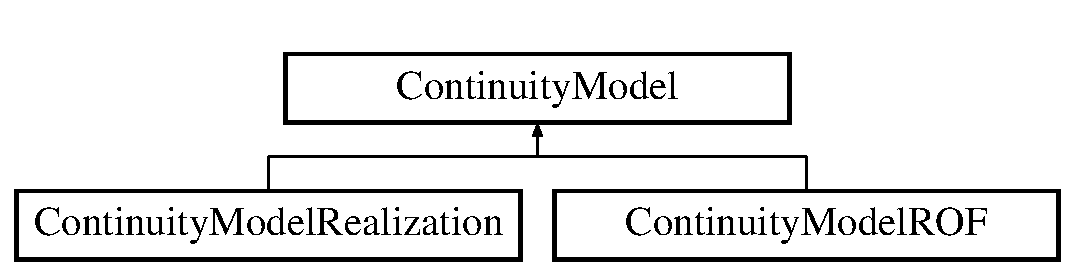
\includegraphics[height=2.000000cm]{classContinuityModel}
\end{center}
\end{figure}
\subsection*{Public Member Functions}
\begin{DoxyCompactItemize}
\item 
\mbox{\hyperlink{classContinuityModel_acadf595deb924bc08c9b702adf223365}{Continuity\+Model}} (vector$<$ \mbox{\hyperlink{classWaterSource}{Water\+Source}} $\ast$$>$ \&water\+\_\+sources, vector$<$ \mbox{\hyperlink{classUtility}{Utility}} $\ast$$>$ \&utilities, vector$<$ Min\+Env\+Flow\+Control $\ast$$>$ \&\mbox{\hyperlink{classContinuityModel_afc991e5c0d144020e49a97751a04b302}{min\+\_\+env\+\_\+flow\+\_\+controls}}, const Graph \&\mbox{\hyperlink{classContinuityModel_a563401588c6fa622f03393909a3522db}{water\+\_\+sources\+\_\+graph}}, const vector$<$ vector$<$ int $>$$>$ \&\mbox{\hyperlink{classContinuityModel_ae8516bcbbf52650190277fc8b06c1843}{water\+\_\+sources\+\_\+to\+\_\+utilities}}, vector$<$ double $>$ \&\mbox{\hyperlink{classContinuityModel_aa4a00b76da6295d2faa11e3dcaea1896}{utilities\+\_\+rdm}}, vector$<$ double $>$ \&\mbox{\hyperlink{classContinuityModel_ab7b8fa93a6f56b328e425e1ead6cfefa}{water\+\_\+sources\+\_\+rdm}}, unsigned long \mbox{\hyperlink{classContinuityModel_a7b6c99bf256f6c6b633ebb78282f43c7}{realization\+\_\+id}})
\begin{DoxyCompactList}\small\item\em Constructs a \mbox{\hyperlink{classContinuityModel}{Continuity\+Model}} object to simulate water flow and demand. \end{DoxyCompactList}\item 
\mbox{\hyperlink{classContinuityModel_a7f46eb1f937b813226ca7fee96e5fd5c}{Continuity\+Model}} (\mbox{\hyperlink{classContinuityModel}{Continuity\+Model}} \&continuity\+\_\+model)
\begin{DoxyCompactList}\small\item\em Copy constructor for a new Continuity Model object. \end{DoxyCompactList}\item 
virtual \mbox{\hyperlink{classContinuityModel_ae901ce342cd6e49c17994e4910873187}{$\sim$\+Continuity\+Model}} ()
\begin{DoxyCompactList}\small\item\em Destructor for \mbox{\hyperlink{classContinuityModel}{Continuity\+Model}} to clean up dynamically allocated resources. \end{DoxyCompactList}\item 
void \mbox{\hyperlink{classContinuityModel_a7c37fec30b6381ded6150df1b1746953}{continuity\+Step}} (int week, int rof\+\_\+realization=-\/1, bool apply\+\_\+demand\+\_\+buffer=false, bool apply\+\_\+demand\+\_\+projection=false)
\begin{DoxyCompactList}\small\item\em Performs a single step of the continuity calculation for water sources and utilities. \end{DoxyCompactList}\item 
void \mbox{\hyperlink{classContinuityModel_a47504c599955b8193ffab3bd0f328144}{set\+Realization}} (unsigned long \mbox{\hyperlink{classContinuityModel_a7b6c99bf256f6c6b633ebb78282f43c7}{realization\+\_\+id}}, vector$<$ double $>$ \&\mbox{\hyperlink{classContinuityModel_aa4a00b76da6295d2faa11e3dcaea1896}{utilities\+\_\+rdm}}, vector$<$ double $>$ \&\mbox{\hyperlink{classContinuityModel_ab7b8fa93a6f56b328e425e1ead6cfefa}{water\+\_\+sources\+\_\+rdm}})
\begin{DoxyCompactList}\small\item\em Sets the realization ID for utilities, water sources, and minimum environmental flow controls. \end{DoxyCompactList}\item 
vector$<$ int $>$ \mbox{\hyperlink{classContinuityModel_a5682041c22910f1b2a79f30ba56a290d}{get\+Online\+Downstream\+Sources}} ()
\begin{DoxyCompactList}\small\item\em Retrieves a list of online downstream water sources for each water source. \end{DoxyCompactList}\item 
const vector$<$ \mbox{\hyperlink{classWaterSource}{Water\+Source}} $\ast$ $>$ \& \mbox{\hyperlink{classContinuityModel_aa0fbc434152c2ca4fc5e9534fa428de7}{get\+Continuity\+\_\+water\+\_\+sources}} () const
\begin{DoxyCompactList}\small\item\em Retrieves the list of water sources in the continuity model. \end{DoxyCompactList}\item 
const vector$<$ \mbox{\hyperlink{classUtility}{Utility}} $\ast$ $>$ \& \mbox{\hyperlink{classContinuityModel_ac95d9ee421dee12258643c4b7e5caa5d}{get\+Continuity\+\_\+utilities}} () const
\begin{DoxyCompactList}\small\item\em Retrieves the list of utilities in the continuity model. \end{DoxyCompactList}\end{DoxyCompactItemize}
\subsection*{Public Attributes}
\begin{DoxyCompactItemize}
\item 
const unsigned long \mbox{\hyperlink{classContinuityModel_a7b6c99bf256f6c6b633ebb78282f43c7}{realization\+\_\+id}}
\begin{DoxyCompactList}\small\item\em An unsigned long integer representing the realization id. \end{DoxyCompactList}\end{DoxyCompactItemize}
\subsection*{Protected Attributes}
\begin{DoxyCompactItemize}
\item 
vector$<$ \mbox{\hyperlink{classWaterSource}{Water\+Source}} $\ast$ $>$ \mbox{\hyperlink{classContinuityModel_a3980284a9dd08bae4e76398d1b0d6f55}{continuity\+\_\+water\+\_\+sources}}
\begin{DoxyCompactList}\small\item\em A vector of \mbox{\hyperlink{classWaterSource}{Water\+Source}} objects representing the water sources in the system. \end{DoxyCompactList}\item 
vector$<$ \mbox{\hyperlink{classUtility}{Utility}} $\ast$ $>$ \mbox{\hyperlink{classContinuityModel_adc77a0214d553a961035ce86c93cf9be}{continuity\+\_\+utilities}}
\begin{DoxyCompactList}\small\item\em A vector of \mbox{\hyperlink{classUtility}{Utility}} objects representing the utilities in the system. \end{DoxyCompactList}\item 
vector$<$ Min\+Env\+Flow\+Control $\ast$ $>$ \mbox{\hyperlink{classContinuityModel_afc991e5c0d144020e49a97751a04b302}{min\+\_\+env\+\_\+flow\+\_\+controls}}
\begin{DoxyCompactList}\small\item\em A vector of Min\+Env\+Flow\+Control objects representing the minimum environmental flow controls in the system. \end{DoxyCompactList}\item 
Graph \mbox{\hyperlink{classContinuityModel_a563401588c6fa622f03393909a3522db}{water\+\_\+sources\+\_\+graph}}
\begin{DoxyCompactList}\small\item\em A bidirectional Graph object representing the connections between the water sources in the system. \end{DoxyCompactList}\item 
vector$<$ vector$<$ int $>$ $>$ \mbox{\hyperlink{classContinuityModel_ae8516bcbbf52650190277fc8b06c1843}{water\+\_\+sources\+\_\+to\+\_\+utilities}}
\begin{DoxyCompactList}\small\item\em A 2D vector of integers representing the water sources supplying each utility, irrespective of their online/offline status. \end{DoxyCompactList}\item 
vector$<$ vector$<$ int $>$ $>$ \mbox{\hyperlink{classContinuityModel_a6d80a7e50e022e2cdb5e912d5b3b5cf0}{water\+\_\+sources\+\_\+online\+\_\+to\+\_\+utilities}}
\begin{DoxyCompactList}\small\item\em A 2D vector of integers representing the water sources supplying each utility that are is already built and functional. \end{DoxyCompactList}\item 
vector$<$ vector$<$ int $>$ $>$ \mbox{\hyperlink{classContinuityModel_a5cf4be0afa886eb09a3e143f54c29044}{utilities\+\_\+to\+\_\+water\+\_\+sources}}
\begin{DoxyCompactList}\small\item\em A 2D vector of integers representing the utilities that draw water from each water source. \end{DoxyCompactList}\item 
vector$<$ int $>$ \mbox{\hyperlink{classContinuityModel_af00ea62ac8e2e398591ff608c2a203ef}{downstream\+\_\+sources}}
\begin{DoxyCompactList}\small\item\em A vector of integers representing the downstream source of each water source. \end{DoxyCompactList}\item 
const vector$<$ int $>$ \mbox{\hyperlink{classContinuityModel_a6605cb6aae0370eb84d2e8bf7d6d651e}{sources\+\_\+topological\+\_\+order}}
\begin{DoxyCompactList}\small\item\em A vector of integers representing the topological order of each water source. \end{DoxyCompactList}\item 
vector$<$ double $>$ \mbox{\hyperlink{classContinuityModel_aadc8d46b2d0cc0a5c6b5ccdf0c5c24d4}{water\+\_\+sources\+\_\+capacities}}
\begin{DoxyCompactList}\small\item\em A vector of doubles representing the capacities of each water source. \end{DoxyCompactList}\item 
vector$<$ double $>$ \mbox{\hyperlink{classContinuityModel_a781786effdf14fefcb2201eb33d9e0c7}{utilities\+\_\+capacities}}
\begin{DoxyCompactList}\small\item\em A vector of doubles representing the capacities of each utility. \end{DoxyCompactList}\item 
vector$<$ vector$<$ double $>$ $>$ \mbox{\hyperlink{classContinuityModel_a1994ed4d99e0583eac5c82a4b26d9728}{demands}}
\begin{DoxyCompactList}\small\item\em A 2D vector of doubles representing the demand timeseries of each utility. \end{DoxyCompactList}\item 
vector$<$ double $>$ \mbox{\hyperlink{classContinuityModel_aa4a00b76da6295d2faa11e3dcaea1896}{utilities\+\_\+rdm}}
\begin{DoxyCompactList}\small\item\em A vector of doubles representing the DU factor multipliers for each utility\textquotesingle{}s water demands. \end{DoxyCompactList}\item 
vector$<$ double $>$ \mbox{\hyperlink{classContinuityModel_ab7b8fa93a6f56b328e425e1ead6cfefa}{water\+\_\+sources\+\_\+rdm}}
\begin{DoxyCompactList}\small\item\em A vector of doubles representing the DU factor multipliers scaling the construction, permitting, and financing aspects of a water source. \end{DoxyCompactList}\item 
const int \mbox{\hyperlink{classContinuityModel_a6df6198ebc99a099df08f4b8ce6b52b9}{n\+\_\+utilities}}
\begin{DoxyCompactList}\small\item\em An integer representing the number of utilities in the system. \end{DoxyCompactList}\item 
const int \mbox{\hyperlink{classContinuityModel_a3c25a0d17579eb0fdad0b18319441460}{n\+\_\+sources}}
\begin{DoxyCompactList}\small\item\em An integer representing the number of water sources in the system. \end{DoxyCompactList}\item 
int \mbox{\hyperlink{classContinuityModel_aee4088e422a0d3723dc7895c96c9ebe3}{delta\+\_\+realization\+\_\+weeks}} \mbox{[}N\+U\+M\+B\+E\+R\+\_\+\+R\+E\+A\+L\+I\+Z\+A\+T\+I\+O\+N\+S\+\_\+\+R\+OF+1\mbox{]}
\begin{DoxyCompactList}\small\item\em An array of integers representing the number of weeks to be added to the current week to get the actual current week of the realization. \end{DoxyCompactList}\end{DoxyCompactItemize}


\subsection{Constructor \& Destructor Documentation}
\mbox{\Hypertarget{classContinuityModel_acadf595deb924bc08c9b702adf223365}\label{classContinuityModel_acadf595deb924bc08c9b702adf223365}} 
\index{Continuity\+Model@{Continuity\+Model}!Continuity\+Model@{Continuity\+Model}}
\index{Continuity\+Model@{Continuity\+Model}!Continuity\+Model@{Continuity\+Model}}
\subsubsection{\texorpdfstring{Continuity\+Model()}{ContinuityModel()}\hspace{0.1cm}{\footnotesize\ttfamily [1/2]}}
{\footnotesize\ttfamily Continuity\+Model\+::\+Continuity\+Model (\begin{DoxyParamCaption}\item[{vector$<$ \mbox{\hyperlink{classWaterSource}{Water\+Source}} $\ast$$>$ \&}]{water\+\_\+sources,  }\item[{vector$<$ \mbox{\hyperlink{classUtility}{Utility}} $\ast$$>$ \&}]{utilities,  }\item[{vector$<$ Min\+Env\+Flow\+Control $\ast$$>$ \&}]{min\+\_\+env\+\_\+flow\+\_\+controls,  }\item[{const Graph \&}]{water\+\_\+sources\+\_\+graph,  }\item[{const vector$<$ vector$<$ int $>$$>$ \&}]{water\+\_\+sources\+\_\+to\+\_\+utilities,  }\item[{vector$<$ double $>$ \&}]{utilities\+\_\+rdm,  }\item[{vector$<$ double $>$ \&}]{water\+\_\+sources\+\_\+rdm,  }\item[{unsigned long}]{realization\+\_\+id }\end{DoxyParamCaption})}



Constructs a \mbox{\hyperlink{classContinuityModel}{Continuity\+Model}} object to simulate water flow and demand. 

This constructor initializes a continuity model, linking water sources, utilities, and minimum environmental flow controls to simulate water distribution and demand over time. It sets up various internal tables and vectors for faster calculations and ensures proper linking of utilities to water sources. Additionally, it handles initialization for various properties like capacities and realization data.


\begin{DoxyParams}{Parameters}
{\em water\+\_\+sources} & A vector of pointers to the water sources in the model. \\
\hline
{\em utilities} & A vector of pointers to the utilities in the model. \\
\hline
{\em min\+\_\+env\+\_\+flow\+\_\+controls} & A vector of pointers to the minimum environmental flow controls. \\
\hline
{\em water\+\_\+sources\+\_\+graph} & A graph representing the water sources and their relationships. \\
\hline
{\em water\+\_\+sources\+\_\+to\+\_\+utilities} & A matrix mapping each utility to the water sources it uses. \\
\hline
{\em utilities\+\_\+rdm} & A vector of randomization factors for the utilities. \\
\hline
{\em water\+\_\+sources\+\_\+rdm} & A vector of randomization factors for the water sources. \\
\hline
{\em realization\+\_\+id} & An identifier for the current realization.\\
\hline
\end{DoxyParams}

\begin{DoxyExceptions}{Exceptions}
{\em invalid\+\_\+argument} & If any of the water sources are not correctly linked to utilities, or if utilities lack storage capacity, an exception is thrown. \\
\hline
\end{DoxyExceptions}
\mbox{\Hypertarget{classContinuityModel_a7f46eb1f937b813226ca7fee96e5fd5c}\label{classContinuityModel_a7f46eb1f937b813226ca7fee96e5fd5c}} 
\index{Continuity\+Model@{Continuity\+Model}!Continuity\+Model@{Continuity\+Model}}
\index{Continuity\+Model@{Continuity\+Model}!Continuity\+Model@{Continuity\+Model}}
\subsubsection{\texorpdfstring{Continuity\+Model()}{ContinuityModel()}\hspace{0.1cm}{\footnotesize\ttfamily [2/2]}}
{\footnotesize\ttfamily Continuity\+Model\+::\+Continuity\+Model (\begin{DoxyParamCaption}\item[{\mbox{\hyperlink{classContinuityModel}{Continuity\+Model}} \&}]{continuity\+\_\+model }\end{DoxyParamCaption})}



Copy constructor for a new Continuity Model object. 


\begin{DoxyParams}{Parameters}
{\em continuity\+\_\+model} & A reference to the \mbox{\hyperlink{classContinuityModel}{Continuity\+Model}} object to be copied.\\
\hline
\end{DoxyParams}
\begin{DoxyReturn}{Returns}
A new \mbox{\hyperlink{classContinuityModel}{Continuity\+Model}} object with the same properties as the original. 
\end{DoxyReturn}
\mbox{\Hypertarget{classContinuityModel_ae901ce342cd6e49c17994e4910873187}\label{classContinuityModel_ae901ce342cd6e49c17994e4910873187}} 
\index{Continuity\+Model@{Continuity\+Model}!````~Continuity\+Model@{$\sim$\+Continuity\+Model}}
\index{````~Continuity\+Model@{$\sim$\+Continuity\+Model}!Continuity\+Model@{Continuity\+Model}}
\subsubsection{\texorpdfstring{$\sim$\+Continuity\+Model()}{~ContinuityModel()}}
{\footnotesize\ttfamily virtual Continuity\+Model\+::$\sim$\+Continuity\+Model (\begin{DoxyParamCaption}{ }\end{DoxyParamCaption})\hspace{0.3cm}{\ttfamily [virtual]}}



Destructor for \mbox{\hyperlink{classContinuityModel}{Continuity\+Model}} to clean up dynamically allocated resources. 

This destructor is responsible for deleting all dynamically allocated objects associated with the \mbox{\hyperlink{classContinuityModel}{Continuity\+Model}} instance, including water sources, utilities, and minimum environmental flow controls. It ensures proper cleanup to avoid memory leaks when the model is no longer needed.

This is a virtual function meant to be overridden by subclasses to ensure proper cleanup of any additional resources they may have allocated. 

\subsection{Member Function Documentation}
\mbox{\Hypertarget{classContinuityModel_a7c37fec30b6381ded6150df1b1746953}\label{classContinuityModel_a7c37fec30b6381ded6150df1b1746953}} 
\index{Continuity\+Model@{Continuity\+Model}!continuity\+Step@{continuity\+Step}}
\index{continuity\+Step@{continuity\+Step}!Continuity\+Model@{Continuity\+Model}}
\subsubsection{\texorpdfstring{continuity\+Step()}{continuityStep()}}
{\footnotesize\ttfamily void Continuity\+Model\+::continuity\+Step (\begin{DoxyParamCaption}\item[{int}]{week,  }\item[{int}]{rof\+\_\+realization = {\ttfamily -\/1},  }\item[{bool}]{apply\+\_\+demand\+\_\+buffer = {\ttfamily false},  }\item[{bool}]{apply\+\_\+demand\+\_\+projection = {\ttfamily false} }\end{DoxyParamCaption})}



Performs a single step of the continuity calculation for water sources and utilities. 

This function performs a mass balance calculation for each water source in the continuity model, updating the available volume and accounting for upstream spillage, wastewater discharges, and demand projections. It also updates the minimum environmental flows and utility storage volumes.


\begin{DoxyParams}{Parameters}
{\em week} & The current week of the simulation. \\
\hline
{\em rof\+\_\+realization} & The realization index for the R\+OF calculation (use {\ttfamily N\+O\+N\+\_\+\+I\+N\+I\+T\+I\+A\+L\+I\+Z\+ED} for a regular simulation). \\
\hline
{\em apply\+\_\+demand\+\_\+buffer} & Flag to indicate whether to apply the demand buffer to the simulation. \\
\hline
{\em apply\+\_\+demand\+\_\+projection} & Flag to indicate whether to apply the demand projection to the simulation.\\
\hline
\end{DoxyParams}
\begin{DoxyReturn}{Returns}
void 
\end{DoxyReturn}
\mbox{\Hypertarget{classContinuityModel_ac95d9ee421dee12258643c4b7e5caa5d}\label{classContinuityModel_ac95d9ee421dee12258643c4b7e5caa5d}} 
\index{Continuity\+Model@{Continuity\+Model}!get\+Continuity\+\_\+utilities@{get\+Continuity\+\_\+utilities}}
\index{get\+Continuity\+\_\+utilities@{get\+Continuity\+\_\+utilities}!Continuity\+Model@{Continuity\+Model}}
\subsubsection{\texorpdfstring{get\+Continuity\+\_\+utilities()}{getContinuity\_utilities()}}
{\footnotesize\ttfamily const vector$<$\mbox{\hyperlink{classUtility}{Utility}} $\ast$$>$\& Continuity\+Model\+::get\+Continuity\+\_\+utilities (\begin{DoxyParamCaption}{ }\end{DoxyParamCaption}) const}



Retrieves the list of utilities in the continuity model. 

This function returns a constant reference to the vector of utilities that are included in the continuity model. The utilities represent all entities that rely on the water sources for their operations in the model\textquotesingle{}s calculations.

\begin{DoxyReturn}{Returns}
A constant reference to the vector of {\ttfamily \mbox{\hyperlink{classUtility}{Utility}}} pointers. 
\end{DoxyReturn}
\mbox{\Hypertarget{classContinuityModel_aa0fbc434152c2ca4fc5e9534fa428de7}\label{classContinuityModel_aa0fbc434152c2ca4fc5e9534fa428de7}} 
\index{Continuity\+Model@{Continuity\+Model}!get\+Continuity\+\_\+water\+\_\+sources@{get\+Continuity\+\_\+water\+\_\+sources}}
\index{get\+Continuity\+\_\+water\+\_\+sources@{get\+Continuity\+\_\+water\+\_\+sources}!Continuity\+Model@{Continuity\+Model}}
\subsubsection{\texorpdfstring{get\+Continuity\+\_\+water\+\_\+sources()}{getContinuity\_water\_sources()}}
{\footnotesize\ttfamily const vector$<$\mbox{\hyperlink{classWaterSource}{Water\+Source}} $\ast$$>$\& Continuity\+Model\+::get\+Continuity\+\_\+water\+\_\+sources (\begin{DoxyParamCaption}{ }\end{DoxyParamCaption}) const}



Retrieves the list of water sources in the continuity model. 

This function returns a constant reference to the vector of water sources that are included in the continuity model. The water sources represent all sources involved in the model\textquotesingle{}s calculations for continuity.

\begin{DoxyReturn}{Returns}
A constant reference to the vector of {\ttfamily \mbox{\hyperlink{classWaterSource}{Water\+Source}}} pointers. 
\end{DoxyReturn}
\mbox{\Hypertarget{classContinuityModel_a5682041c22910f1b2a79f30ba56a290d}\label{classContinuityModel_a5682041c22910f1b2a79f30ba56a290d}} 
\index{Continuity\+Model@{Continuity\+Model}!get\+Online\+Downstream\+Sources@{get\+Online\+Downstream\+Sources}}
\index{get\+Online\+Downstream\+Sources@{get\+Online\+Downstream\+Sources}!Continuity\+Model@{Continuity\+Model}}
\subsubsection{\texorpdfstring{get\+Online\+Downstream\+Sources()}{getOnlineDownstreamSources()}}
{\footnotesize\ttfamily vector$<$int$>$ Continuity\+Model\+::get\+Online\+Downstream\+Sources (\begin{DoxyParamCaption}{ }\end{DoxyParamCaption})}



Retrieves a list of online downstream water sources for each water source. 

This function iterates through the water sources in topological order and identifies the first online downstream source for each water source. The result is a vector where each element represents the first online downstream source for the corresponding water source, or {\ttfamily N\+O\+N\+\_\+\+I\+N\+I\+T\+I\+A\+L\+I\+Z\+ED} if no online downstream source is found.

\begin{DoxyReturn}{Returns}
A vector of integers representing the I\+Ds of the online downstream sources for each water source. 
\end{DoxyReturn}
\mbox{\Hypertarget{classContinuityModel_a47504c599955b8193ffab3bd0f328144}\label{classContinuityModel_a47504c599955b8193ffab3bd0f328144}} 
\index{Continuity\+Model@{Continuity\+Model}!set\+Realization@{set\+Realization}}
\index{set\+Realization@{set\+Realization}!Continuity\+Model@{Continuity\+Model}}
\subsubsection{\texorpdfstring{set\+Realization()}{setRealization()}}
{\footnotesize\ttfamily void Continuity\+Model\+::set\+Realization (\begin{DoxyParamCaption}\item[{unsigned long}]{realization\+\_\+id,  }\item[{vector$<$ double $>$ \&}]{utilities\+\_\+rdm,  }\item[{vector$<$ double $>$ \&}]{water\+\_\+sources\+\_\+rdm }\end{DoxyParamCaption})}



Sets the realization ID for utilities, water sources, and minimum environmental flow controls. 

This function assigns a specific realization ID to each utility, water source, and minimum environmental flow control in the continuity model. This ensures that the correct realization data is used for the simulation.


\begin{DoxyParams}{Parameters}
{\em realization\+\_\+id} & The ID of the realization to be set. \\
\hline
{\em utilities\+\_\+rdm} & A vector containing random demand values for each utility, indexed by utility ID. \\
\hline
{\em water\+\_\+sources\+\_\+rdm} & A vector containing random demand values for each water source, indexed by source ID.\\
\hline
\end{DoxyParams}
\begin{DoxyReturn}{Returns}
void 
\end{DoxyReturn}


\subsection{Member Data Documentation}
\mbox{\Hypertarget{classContinuityModel_adc77a0214d553a961035ce86c93cf9be}\label{classContinuityModel_adc77a0214d553a961035ce86c93cf9be}} 
\index{Continuity\+Model@{Continuity\+Model}!continuity\+\_\+utilities@{continuity\+\_\+utilities}}
\index{continuity\+\_\+utilities@{continuity\+\_\+utilities}!Continuity\+Model@{Continuity\+Model}}
\subsubsection{\texorpdfstring{continuity\+\_\+utilities}{continuity\_utilities}}
{\footnotesize\ttfamily vector$<$\mbox{\hyperlink{classUtility}{Utility}} $\ast$$>$ Continuity\+Model\+::continuity\+\_\+utilities\hspace{0.3cm}{\ttfamily [protected]}}



A vector of \mbox{\hyperlink{classUtility}{Utility}} objects representing the utilities in the system. 

\mbox{\Hypertarget{classContinuityModel_a3980284a9dd08bae4e76398d1b0d6f55}\label{classContinuityModel_a3980284a9dd08bae4e76398d1b0d6f55}} 
\index{Continuity\+Model@{Continuity\+Model}!continuity\+\_\+water\+\_\+sources@{continuity\+\_\+water\+\_\+sources}}
\index{continuity\+\_\+water\+\_\+sources@{continuity\+\_\+water\+\_\+sources}!Continuity\+Model@{Continuity\+Model}}
\subsubsection{\texorpdfstring{continuity\+\_\+water\+\_\+sources}{continuity\_water\_sources}}
{\footnotesize\ttfamily vector$<$\mbox{\hyperlink{classWaterSource}{Water\+Source}} $\ast$$>$ Continuity\+Model\+::continuity\+\_\+water\+\_\+sources\hspace{0.3cm}{\ttfamily [protected]}}



A vector of \mbox{\hyperlink{classWaterSource}{Water\+Source}} objects representing the water sources in the system. 

\mbox{\Hypertarget{classContinuityModel_aee4088e422a0d3723dc7895c96c9ebe3}\label{classContinuityModel_aee4088e422a0d3723dc7895c96c9ebe3}} 
\index{Continuity\+Model@{Continuity\+Model}!delta\+\_\+realization\+\_\+weeks@{delta\+\_\+realization\+\_\+weeks}}
\index{delta\+\_\+realization\+\_\+weeks@{delta\+\_\+realization\+\_\+weeks}!Continuity\+Model@{Continuity\+Model}}
\subsubsection{\texorpdfstring{delta\+\_\+realization\+\_\+weeks}{delta\_realization\_weeks}}
{\footnotesize\ttfamily int Continuity\+Model\+::delta\+\_\+realization\+\_\+weeks\mbox{[}N\+U\+M\+B\+E\+R\+\_\+\+R\+E\+A\+L\+I\+Z\+A\+T\+I\+O\+N\+S\+\_\+\+R\+OF+1\mbox{]}\hspace{0.3cm}{\ttfamily [protected]}}



An array of integers representing the number of weeks to be added to the current week to get the actual current week of the realization. 

\mbox{\Hypertarget{classContinuityModel_a1994ed4d99e0583eac5c82a4b26d9728}\label{classContinuityModel_a1994ed4d99e0583eac5c82a4b26d9728}} 
\index{Continuity\+Model@{Continuity\+Model}!demands@{demands}}
\index{demands@{demands}!Continuity\+Model@{Continuity\+Model}}
\subsubsection{\texorpdfstring{demands}{demands}}
{\footnotesize\ttfamily vector$<$vector$<$double$>$ $>$ Continuity\+Model\+::demands\hspace{0.3cm}{\ttfamily [protected]}}



A 2D vector of doubles representing the demand timeseries of each utility. 

\mbox{\Hypertarget{classContinuityModel_af00ea62ac8e2e398591ff608c2a203ef}\label{classContinuityModel_af00ea62ac8e2e398591ff608c2a203ef}} 
\index{Continuity\+Model@{Continuity\+Model}!downstream\+\_\+sources@{downstream\+\_\+sources}}
\index{downstream\+\_\+sources@{downstream\+\_\+sources}!Continuity\+Model@{Continuity\+Model}}
\subsubsection{\texorpdfstring{downstream\+\_\+sources}{downstream\_sources}}
{\footnotesize\ttfamily vector$<$int$>$ Continuity\+Model\+::downstream\+\_\+sources\hspace{0.3cm}{\ttfamily [protected]}}



A vector of integers representing the downstream source of each water source. 

\mbox{\Hypertarget{classContinuityModel_afc991e5c0d144020e49a97751a04b302}\label{classContinuityModel_afc991e5c0d144020e49a97751a04b302}} 
\index{Continuity\+Model@{Continuity\+Model}!min\+\_\+env\+\_\+flow\+\_\+controls@{min\+\_\+env\+\_\+flow\+\_\+controls}}
\index{min\+\_\+env\+\_\+flow\+\_\+controls@{min\+\_\+env\+\_\+flow\+\_\+controls}!Continuity\+Model@{Continuity\+Model}}
\subsubsection{\texorpdfstring{min\+\_\+env\+\_\+flow\+\_\+controls}{min\_env\_flow\_controls}}
{\footnotesize\ttfamily vector$<$Min\+Env\+Flow\+Control $\ast$$>$ Continuity\+Model\+::min\+\_\+env\+\_\+flow\+\_\+controls\hspace{0.3cm}{\ttfamily [protected]}}



A vector of Min\+Env\+Flow\+Control objects representing the minimum environmental flow controls in the system. 

\mbox{\Hypertarget{classContinuityModel_a3c25a0d17579eb0fdad0b18319441460}\label{classContinuityModel_a3c25a0d17579eb0fdad0b18319441460}} 
\index{Continuity\+Model@{Continuity\+Model}!n\+\_\+sources@{n\+\_\+sources}}
\index{n\+\_\+sources@{n\+\_\+sources}!Continuity\+Model@{Continuity\+Model}}
\subsubsection{\texorpdfstring{n\+\_\+sources}{n\_sources}}
{\footnotesize\ttfamily const int Continuity\+Model\+::n\+\_\+sources\hspace{0.3cm}{\ttfamily [protected]}}



An integer representing the number of water sources in the system. 

\mbox{\Hypertarget{classContinuityModel_a6df6198ebc99a099df08f4b8ce6b52b9}\label{classContinuityModel_a6df6198ebc99a099df08f4b8ce6b52b9}} 
\index{Continuity\+Model@{Continuity\+Model}!n\+\_\+utilities@{n\+\_\+utilities}}
\index{n\+\_\+utilities@{n\+\_\+utilities}!Continuity\+Model@{Continuity\+Model}}
\subsubsection{\texorpdfstring{n\+\_\+utilities}{n\_utilities}}
{\footnotesize\ttfamily const int Continuity\+Model\+::n\+\_\+utilities\hspace{0.3cm}{\ttfamily [protected]}}



An integer representing the number of utilities in the system. 

\mbox{\Hypertarget{classContinuityModel_a7b6c99bf256f6c6b633ebb78282f43c7}\label{classContinuityModel_a7b6c99bf256f6c6b633ebb78282f43c7}} 
\index{Continuity\+Model@{Continuity\+Model}!realization\+\_\+id@{realization\+\_\+id}}
\index{realization\+\_\+id@{realization\+\_\+id}!Continuity\+Model@{Continuity\+Model}}
\subsubsection{\texorpdfstring{realization\+\_\+id}{realization\_id}}
{\footnotesize\ttfamily const unsigned long Continuity\+Model\+::realization\+\_\+id}



An unsigned long integer representing the realization id. 

\mbox{\Hypertarget{classContinuityModel_a6605cb6aae0370eb84d2e8bf7d6d651e}\label{classContinuityModel_a6605cb6aae0370eb84d2e8bf7d6d651e}} 
\index{Continuity\+Model@{Continuity\+Model}!sources\+\_\+topological\+\_\+order@{sources\+\_\+topological\+\_\+order}}
\index{sources\+\_\+topological\+\_\+order@{sources\+\_\+topological\+\_\+order}!Continuity\+Model@{Continuity\+Model}}
\subsubsection{\texorpdfstring{sources\+\_\+topological\+\_\+order}{sources\_topological\_order}}
{\footnotesize\ttfamily const vector$<$int$>$ Continuity\+Model\+::sources\+\_\+topological\+\_\+order\hspace{0.3cm}{\ttfamily [protected]}}



A vector of integers representing the topological order of each water source. 

\mbox{\Hypertarget{classContinuityModel_a781786effdf14fefcb2201eb33d9e0c7}\label{classContinuityModel_a781786effdf14fefcb2201eb33d9e0c7}} 
\index{Continuity\+Model@{Continuity\+Model}!utilities\+\_\+capacities@{utilities\+\_\+capacities}}
\index{utilities\+\_\+capacities@{utilities\+\_\+capacities}!Continuity\+Model@{Continuity\+Model}}
\subsubsection{\texorpdfstring{utilities\+\_\+capacities}{utilities\_capacities}}
{\footnotesize\ttfamily vector$<$double$>$ Continuity\+Model\+::utilities\+\_\+capacities\hspace{0.3cm}{\ttfamily [protected]}}



A vector of doubles representing the capacities of each utility. 

\mbox{\Hypertarget{classContinuityModel_aa4a00b76da6295d2faa11e3dcaea1896}\label{classContinuityModel_aa4a00b76da6295d2faa11e3dcaea1896}} 
\index{Continuity\+Model@{Continuity\+Model}!utilities\+\_\+rdm@{utilities\+\_\+rdm}}
\index{utilities\+\_\+rdm@{utilities\+\_\+rdm}!Continuity\+Model@{Continuity\+Model}}
\subsubsection{\texorpdfstring{utilities\+\_\+rdm}{utilities\_rdm}}
{\footnotesize\ttfamily vector$<$double$>$ Continuity\+Model\+::utilities\+\_\+rdm\hspace{0.3cm}{\ttfamily [protected]}}



A vector of doubles representing the DU factor multipliers for each utility\textquotesingle{}s water demands. 

\mbox{\Hypertarget{classContinuityModel_a5cf4be0afa886eb09a3e143f54c29044}\label{classContinuityModel_a5cf4be0afa886eb09a3e143f54c29044}} 
\index{Continuity\+Model@{Continuity\+Model}!utilities\+\_\+to\+\_\+water\+\_\+sources@{utilities\+\_\+to\+\_\+water\+\_\+sources}}
\index{utilities\+\_\+to\+\_\+water\+\_\+sources@{utilities\+\_\+to\+\_\+water\+\_\+sources}!Continuity\+Model@{Continuity\+Model}}
\subsubsection{\texorpdfstring{utilities\+\_\+to\+\_\+water\+\_\+sources}{utilities\_to\_water\_sources}}
{\footnotesize\ttfamily vector$<$vector$<$int$>$ $>$ Continuity\+Model\+::utilities\+\_\+to\+\_\+water\+\_\+sources\hspace{0.3cm}{\ttfamily [protected]}}



A 2D vector of integers representing the utilities that draw water from each water source. 

\mbox{\Hypertarget{classContinuityModel_aadc8d46b2d0cc0a5c6b5ccdf0c5c24d4}\label{classContinuityModel_aadc8d46b2d0cc0a5c6b5ccdf0c5c24d4}} 
\index{Continuity\+Model@{Continuity\+Model}!water\+\_\+sources\+\_\+capacities@{water\+\_\+sources\+\_\+capacities}}
\index{water\+\_\+sources\+\_\+capacities@{water\+\_\+sources\+\_\+capacities}!Continuity\+Model@{Continuity\+Model}}
\subsubsection{\texorpdfstring{water\+\_\+sources\+\_\+capacities}{water\_sources\_capacities}}
{\footnotesize\ttfamily vector$<$double$>$ Continuity\+Model\+::water\+\_\+sources\+\_\+capacities\hspace{0.3cm}{\ttfamily [protected]}}



A vector of doubles representing the capacities of each water source. 

\mbox{\Hypertarget{classContinuityModel_a563401588c6fa622f03393909a3522db}\label{classContinuityModel_a563401588c6fa622f03393909a3522db}} 
\index{Continuity\+Model@{Continuity\+Model}!water\+\_\+sources\+\_\+graph@{water\+\_\+sources\+\_\+graph}}
\index{water\+\_\+sources\+\_\+graph@{water\+\_\+sources\+\_\+graph}!Continuity\+Model@{Continuity\+Model}}
\subsubsection{\texorpdfstring{water\+\_\+sources\+\_\+graph}{water\_sources\_graph}}
{\footnotesize\ttfamily Graph Continuity\+Model\+::water\+\_\+sources\+\_\+graph\hspace{0.3cm}{\ttfamily [protected]}}



A bidirectional Graph object representing the connections between the water sources in the system. 

\mbox{\Hypertarget{classContinuityModel_a6d80a7e50e022e2cdb5e912d5b3b5cf0}\label{classContinuityModel_a6d80a7e50e022e2cdb5e912d5b3b5cf0}} 
\index{Continuity\+Model@{Continuity\+Model}!water\+\_\+sources\+\_\+online\+\_\+to\+\_\+utilities@{water\+\_\+sources\+\_\+online\+\_\+to\+\_\+utilities}}
\index{water\+\_\+sources\+\_\+online\+\_\+to\+\_\+utilities@{water\+\_\+sources\+\_\+online\+\_\+to\+\_\+utilities}!Continuity\+Model@{Continuity\+Model}}
\subsubsection{\texorpdfstring{water\+\_\+sources\+\_\+online\+\_\+to\+\_\+utilities}{water\_sources\_online\_to\_utilities}}
{\footnotesize\ttfamily vector$<$vector$<$int$>$ $>$ Continuity\+Model\+::water\+\_\+sources\+\_\+online\+\_\+to\+\_\+utilities\hspace{0.3cm}{\ttfamily [protected]}}



A 2D vector of integers representing the water sources supplying each utility that are is already built and functional. 

\mbox{\Hypertarget{classContinuityModel_ab7b8fa93a6f56b328e425e1ead6cfefa}\label{classContinuityModel_ab7b8fa93a6f56b328e425e1ead6cfefa}} 
\index{Continuity\+Model@{Continuity\+Model}!water\+\_\+sources\+\_\+rdm@{water\+\_\+sources\+\_\+rdm}}
\index{water\+\_\+sources\+\_\+rdm@{water\+\_\+sources\+\_\+rdm}!Continuity\+Model@{Continuity\+Model}}
\subsubsection{\texorpdfstring{water\+\_\+sources\+\_\+rdm}{water\_sources\_rdm}}
{\footnotesize\ttfamily vector$<$double$>$ Continuity\+Model\+::water\+\_\+sources\+\_\+rdm\hspace{0.3cm}{\ttfamily [protected]}}



A vector of doubles representing the DU factor multipliers scaling the construction, permitting, and financing aspects of a water source. 

\mbox{\Hypertarget{classContinuityModel_ae8516bcbbf52650190277fc8b06c1843}\label{classContinuityModel_ae8516bcbbf52650190277fc8b06c1843}} 
\index{Continuity\+Model@{Continuity\+Model}!water\+\_\+sources\+\_\+to\+\_\+utilities@{water\+\_\+sources\+\_\+to\+\_\+utilities}}
\index{water\+\_\+sources\+\_\+to\+\_\+utilities@{water\+\_\+sources\+\_\+to\+\_\+utilities}!Continuity\+Model@{Continuity\+Model}}
\subsubsection{\texorpdfstring{water\+\_\+sources\+\_\+to\+\_\+utilities}{water\_sources\_to\_utilities}}
{\footnotesize\ttfamily vector$<$vector$<$int$>$ $>$ Continuity\+Model\+::water\+\_\+sources\+\_\+to\+\_\+utilities\hspace{0.3cm}{\ttfamily [protected]}}



A 2D vector of integers representing the water sources supplying each utility, irrespective of their online/offline status. 



The documentation for this class was generated from the following file\+:\begin{DoxyCompactItemize}
\item 
/home/fs02/pmr82\+\_\+0001/lbl59/\+Water\+Paths-\/doc/src/\+Continuity\+Models/\+Base/\mbox{\hyperlink{ContinuityModel_8h}{Continuity\+Model.\+h}}\end{DoxyCompactItemize}

\hypertarget{classContinuityModelRealization}{}\section{Continuity\+Model\+Realization Class Reference}
\label{classContinuityModelRealization}\index{Continuity\+Model\+Realization@{Continuity\+Model\+Realization}}


{\ttfamily \#include $<$Continuity\+Model\+Realization.\+h$>$}

Inheritance diagram for Continuity\+Model\+Realization\+:\begin{figure}[H]
\begin{center}
\leavevmode
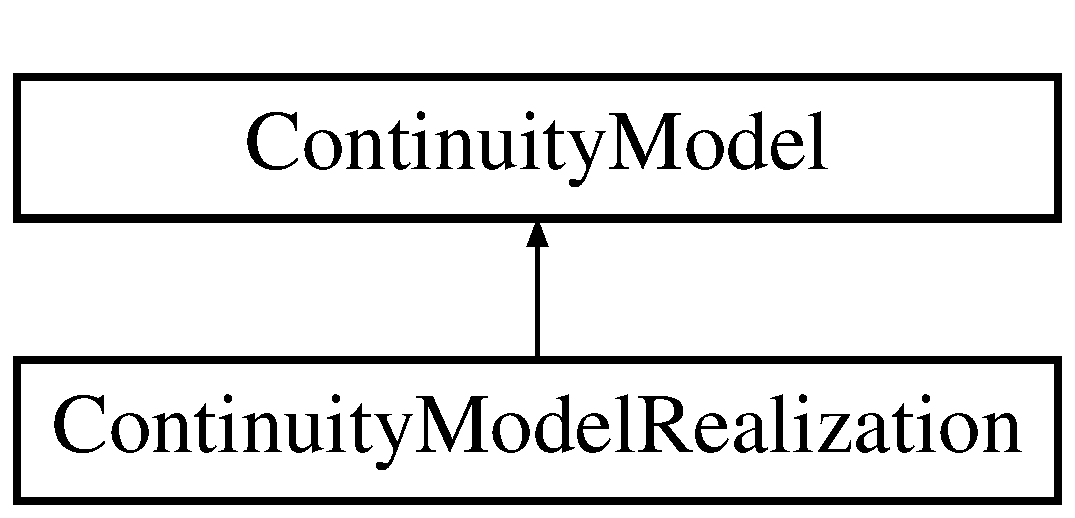
\includegraphics[height=2.000000cm]{classContinuityModelRealization}
\end{center}
\end{figure}
\subsection*{Public Member Functions}
\begin{DoxyCompactItemize}
\item 
\mbox{\hyperlink{classContinuityModelRealization_a641c096ac73586597b3e21a5d516c923}{Continuity\+Model\+Realization}} (vector$<$ \mbox{\hyperlink{classWaterSource}{Water\+Source}} $\ast$$>$ \&water\+\_\+sources, const Graph \&\mbox{\hyperlink{classContinuityModel_a563401588c6fa622f03393909a3522db}{water\+\_\+sources\+\_\+graph}}, const vector$<$ vector$<$ int $>$$>$ \&\mbox{\hyperlink{classContinuityModel_ae8516bcbbf52650190277fc8b06c1843}{water\+\_\+sources\+\_\+to\+\_\+utilities}}, vector$<$ \mbox{\hyperlink{classUtility}{Utility}} $\ast$$>$ \&utilities, const vector$<$ Drought\+Mitigation\+Policy $\ast$$>$ \&\mbox{\hyperlink{classContinuityModelRealization_a757dcf1de115c674fd5adcb040c5f277}{drought\+\_\+mitigation\+\_\+policies}}, vector$<$ Min\+Env\+Flow\+Control $\ast$$>$ \&min\+\_\+env\+\_\+flow\+\_\+control, vector$<$ double $>$ \&\mbox{\hyperlink{classContinuityModel_aa4a00b76da6295d2faa11e3dcaea1896}{utilities\+\_\+rdm}}, vector$<$ double $>$ \&\mbox{\hyperlink{classContinuityModel_ab7b8fa93a6f56b328e425e1ead6cfefa}{water\+\_\+sources\+\_\+rdm}}, vector$<$ double $>$ \&policy\+\_\+rdm, const unsigned int realization\+\_\+index)
\begin{DoxyCompactList}\small\item\em Constructs a \mbox{\hyperlink{classContinuityModelRealization}{Continuity\+Model\+Realization}} object. \end{DoxyCompactList}\item 
\mbox{\hyperlink{classContinuityModelRealization_afd53069e2f9ab96210ff153d16f01269}{$\sim$\+Continuity\+Model\+Realization}} () override
\begin{DoxyCompactList}\small\item\em Destructor for the \mbox{\hyperlink{classContinuityModelRealization}{Continuity\+Model\+Realization}} class. \end{DoxyCompactList}\item 
void \mbox{\hyperlink{classContinuityModelRealization_ae2c40328beb671fa9b10ecc2921b8375}{set\+Short\+Term\+R\+O\+Fs}} (const vector$<$ vector$<$ double $>$$>$ \&risks\+\_\+of\+\_\+failure)
\begin{DoxyCompactList}\small\item\em Sets the short-\/term risks of failure (R\+O\+Fs) for utilities. \end{DoxyCompactList}\item 
void \mbox{\hyperlink{classContinuityModelRealization_a1841f4ca49c150cf5d790f6d42496575}{apply\+Drought\+Mitigation\+Policies}} (int week)
\begin{DoxyCompactList}\small\item\em Applies drought mitigation policies for the given week. \end{DoxyCompactList}\item 
const vector$<$ Drought\+Mitigation\+Policy $\ast$ $>$ \mbox{\hyperlink{classContinuityModelRealization_afadb3e7f51ae7a09948ffc73d7eb7f6b}{get\+Drought\+\_\+mitigation\+\_\+policies}} () const
\begin{DoxyCompactList}\small\item\em Retrieves the drought mitigation policies associated with the continuity model realization. \end{DoxyCompactList}\item 
void \mbox{\hyperlink{classContinuityModelRealization_aa0168985144d26e1613cf20335affedb}{set\+Long\+Term\+R\+O\+Fs}} (const vector$<$ vector$<$ double $>$$>$ \&risks\+\_\+of\+\_\+failure, const int week)
\begin{DoxyCompactList}\small\item\em Sets the long-\/term risks of failure (R\+O\+Fs) for utilities and triggers new infrastructure construction if necessary. \end{DoxyCompactList}\item 
void \mbox{\hyperlink{classContinuityModelRealization_a5b9405156e8cc21c8781ea15ee46c8fe}{set\+Long\+Term\+R\+O\+F\+Demand\+Projection\+Estimate}} (const vector$<$ \mbox{\hyperlink{classUtility}{Utility}} $\ast$$>$ \&rof\+\_\+utilities)
\begin{DoxyCompactList}\small\item\em Updates the demand projection estimates for utilities based on risk of failure (R\+OF) utilities. \end{DoxyCompactList}\item 
void \mbox{\hyperlink{classContinuityModelRealization_ab87c140eaf87266ca81636059e948bb7}{update\+Joint\+W\+T\+P\+Treatment\+Allocations}} (int current\+\_\+week)
\begin{DoxyCompactList}\small\item\em Updates treatment capacity allocations for Joint Water Treatment Plants (W\+T\+Ps) under variable allocation agreements. \end{DoxyCompactList}\end{DoxyCompactItemize}
\subsection*{Private Attributes}
\begin{DoxyCompactItemize}
\item 
vector$<$ Drought\+Mitigation\+Policy $\ast$ $>$ \mbox{\hyperlink{classContinuityModelRealization_a757dcf1de115c674fd5adcb040c5f277}{drought\+\_\+mitigation\+\_\+policies}}
\begin{DoxyCompactList}\small\item\em A vector of pointers to the drought mitigation policies in the system. \end{DoxyCompactList}\end{DoxyCompactItemize}
\subsection*{Additional Inherited Members}


\subsection{Detailed Description}
The \mbox{\hyperlink{classContinuityModelRealization}{Continuity\+Model\+Realization}} class extends the \mbox{\hyperlink{classContinuityModel}{Continuity\+Model}} class to include the implementation of drought mitigation policies and the setting of short-\/term and long-\/term risks of failure.

Created by bernardo on 1/26/17. 

\subsection{Constructor \& Destructor Documentation}
\mbox{\Hypertarget{classContinuityModelRealization_a641c096ac73586597b3e21a5d516c923}\label{classContinuityModelRealization_a641c096ac73586597b3e21a5d516c923}} 
\index{Continuity\+Model\+Realization@{Continuity\+Model\+Realization}!Continuity\+Model\+Realization@{Continuity\+Model\+Realization}}
\index{Continuity\+Model\+Realization@{Continuity\+Model\+Realization}!Continuity\+Model\+Realization@{Continuity\+Model\+Realization}}
\subsubsection{\texorpdfstring{Continuity\+Model\+Realization()}{ContinuityModelRealization()}}
{\footnotesize\ttfamily Continuity\+Model\+Realization\+::\+Continuity\+Model\+Realization (\begin{DoxyParamCaption}\item[{vector$<$ \mbox{\hyperlink{classWaterSource}{Water\+Source}} $\ast$$>$ \&}]{water\+\_\+sources,  }\item[{const Graph \&}]{water\+\_\+sources\+\_\+graph,  }\item[{const vector$<$ vector$<$ int $>$$>$ \&}]{water\+\_\+sources\+\_\+to\+\_\+utilities,  }\item[{vector$<$ \mbox{\hyperlink{classUtility}{Utility}} $\ast$$>$ \&}]{utilities,  }\item[{const vector$<$ Drought\+Mitigation\+Policy $\ast$$>$ \&}]{drought\+\_\+mitigation\+\_\+policies,  }\item[{vector$<$ Min\+Env\+Flow\+Control $\ast$$>$ \&}]{min\+\_\+env\+\_\+flow\+\_\+control,  }\item[{vector$<$ double $>$ \&}]{utilities\+\_\+rdm,  }\item[{vector$<$ double $>$ \&}]{water\+\_\+sources\+\_\+rdm,  }\item[{vector$<$ double $>$ \&}]{policy\+\_\+rdm,  }\item[{const unsigned int}]{realization\+\_\+index }\end{DoxyParamCaption})}



Constructs a \mbox{\hyperlink{classContinuityModelRealization}{Continuity\+Model\+Realization}} object. 

This constructor initializes a {\ttfamily \mbox{\hyperlink{classContinuityModelRealization}{Continuity\+Model\+Realization}}} object, which builds upon the {\ttfamily \mbox{\hyperlink{classContinuityModel}{Continuity\+Model}}} by incorporating drought mitigation policies. It initializes a \mbox{\hyperlink{classContinuityModelRealization}{Continuity\+Model\+Realization}} object by calling the \mbox{\hyperlink{classContinuityModel}{Continuity\+Model}} constructor, adding susytem components to the drought mitigation policies. It also sets the realization for each drought mitigation policy with the provided realization data.


\begin{DoxyParams}{Parameters}
{\em water\+\_\+sources} & A vector of {\ttfamily \mbox{\hyperlink{classWaterSource}{Water\+Source}}} pointers representing the water sources involved in the model. \\
\hline
{\em water\+\_\+sources\+\_\+graph} & A {\ttfamily Graph} representing the relationships and connections between the water sources. \\
\hline
{\em water\+\_\+sources\+\_\+to\+\_\+utilities} & A 2D vector indicating which water sources are connected to which utilities. \\
\hline
{\em utilities} & A vector of {\ttfamily \mbox{\hyperlink{classUtility}{Utility}}} pointers representing the utilities that rely on the water sources. \\
\hline
{\em drought\+\_\+mitigation\+\_\+policies} & A vector of {\ttfamily Drought\+Mitigation\+Policy} pointers, each representing a policy for managing drought conditions. \\
\hline
{\em min\+\_\+env\+\_\+flow\+\_\+control} & A vector of {\ttfamily Min\+Env\+Flow\+Control} pointers used to set minimum environmental flows for water sources. \\
\hline
{\em utilities\+\_\+rdm} & A vector containing random demand values for the utilities in the model. \\
\hline
{\em water\+\_\+sources\+\_\+rdm} & A vector containing random demand values for the water sources in the model. \\
\hline
{\em policy\+\_\+rdm} & A vector containing random demand values for the drought mitigation policies. \\
\hline
{\em realization\+\_\+id} & The realization identifier used to associate a specific realization of the model.\\
\hline
\end{DoxyParams}
\begin{DoxyReturn}{Returns}
A {\ttfamily \mbox{\hyperlink{classContinuityModelRealization}{Continuity\+Model\+Realization}}} object initialized with the provided components and realization. 
\end{DoxyReturn}
\mbox{\Hypertarget{classContinuityModelRealization_afd53069e2f9ab96210ff153d16f01269}\label{classContinuityModelRealization_afd53069e2f9ab96210ff153d16f01269}} 
\index{Continuity\+Model\+Realization@{Continuity\+Model\+Realization}!````~Continuity\+Model\+Realization@{$\sim$\+Continuity\+Model\+Realization}}
\index{````~Continuity\+Model\+Realization@{$\sim$\+Continuity\+Model\+Realization}!Continuity\+Model\+Realization@{Continuity\+Model\+Realization}}
\subsubsection{\texorpdfstring{$\sim$\+Continuity\+Model\+Realization()}{~ContinuityModelRealization()}}
{\footnotesize\ttfamily Continuity\+Model\+Realization\+::$\sim$\+Continuity\+Model\+Realization (\begin{DoxyParamCaption}{ }\end{DoxyParamCaption})\hspace{0.3cm}{\ttfamily [override]}}



Destructor for the \mbox{\hyperlink{classContinuityModelRealization}{Continuity\+Model\+Realization}} class. 

This function releases the memory allocated for drought mitigation policies. It ensures proper cleanup of resources associated with the {\ttfamily \mbox{\hyperlink{classContinuityModelRealization}{Continuity\+Model\+Realization}}} object. 

\subsection{Member Function Documentation}
\mbox{\Hypertarget{classContinuityModelRealization_a1841f4ca49c150cf5d790f6d42496575}\label{classContinuityModelRealization_a1841f4ca49c150cf5d790f6d42496575}} 
\index{Continuity\+Model\+Realization@{Continuity\+Model\+Realization}!apply\+Drought\+Mitigation\+Policies@{apply\+Drought\+Mitigation\+Policies}}
\index{apply\+Drought\+Mitigation\+Policies@{apply\+Drought\+Mitigation\+Policies}!Continuity\+Model\+Realization@{Continuity\+Model\+Realization}}
\subsubsection{\texorpdfstring{apply\+Drought\+Mitigation\+Policies()}{applyDroughtMitigationPolicies()}}
{\footnotesize\ttfamily void Continuity\+Model\+Realization\+::apply\+Drought\+Mitigation\+Policies (\begin{DoxyParamCaption}\item[{int}]{week }\end{DoxyParamCaption})}



Applies drought mitigation policies for the given week. 

This function iterates through all the drought mitigation policies and applies each policy to the system for the specified week.


\begin{DoxyParams}{Parameters}
{\em week} & The current week for which drought mitigation policies are to be applied.\\
\hline
\end{DoxyParams}
\begin{DoxyReturn}{Returns}
void 
\end{DoxyReturn}
\mbox{\Hypertarget{classContinuityModelRealization_afadb3e7f51ae7a09948ffc73d7eb7f6b}\label{classContinuityModelRealization_afadb3e7f51ae7a09948ffc73d7eb7f6b}} 
\index{Continuity\+Model\+Realization@{Continuity\+Model\+Realization}!get\+Drought\+\_\+mitigation\+\_\+policies@{get\+Drought\+\_\+mitigation\+\_\+policies}}
\index{get\+Drought\+\_\+mitigation\+\_\+policies@{get\+Drought\+\_\+mitigation\+\_\+policies}!Continuity\+Model\+Realization@{Continuity\+Model\+Realization}}
\subsubsection{\texorpdfstring{get\+Drought\+\_\+mitigation\+\_\+policies()}{getDrought\_mitigation\_policies()}}
{\footnotesize\ttfamily const vector$<$Drought\+Mitigation\+Policy $\ast$$>$ Continuity\+Model\+Realization\+::get\+Drought\+\_\+mitigation\+\_\+policies (\begin{DoxyParamCaption}{ }\end{DoxyParamCaption}) const}



Retrieves the drought mitigation policies associated with the continuity model realization. 

This function returns a vector containing pointers to all drought mitigation policies in the system.

\begin{DoxyReturn}{Returns}
A {\ttfamily vector} of pointers to {\ttfamily Drought\+Mitigation\+Policy} objects associated with the continuity model realization. 
\end{DoxyReturn}
\mbox{\Hypertarget{classContinuityModelRealization_a5b9405156e8cc21c8781ea15ee46c8fe}\label{classContinuityModelRealization_a5b9405156e8cc21c8781ea15ee46c8fe}} 
\index{Continuity\+Model\+Realization@{Continuity\+Model\+Realization}!set\+Long\+Term\+R\+O\+F\+Demand\+Projection\+Estimate@{set\+Long\+Term\+R\+O\+F\+Demand\+Projection\+Estimate}}
\index{set\+Long\+Term\+R\+O\+F\+Demand\+Projection\+Estimate@{set\+Long\+Term\+R\+O\+F\+Demand\+Projection\+Estimate}!Continuity\+Model\+Realization@{Continuity\+Model\+Realization}}
\subsubsection{\texorpdfstring{set\+Long\+Term\+R\+O\+F\+Demand\+Projection\+Estimate()}{setLongTermROFDemandProjectionEstimate()}}
{\footnotesize\ttfamily void Continuity\+Model\+Realization\+::set\+Long\+Term\+R\+O\+F\+Demand\+Projection\+Estimate (\begin{DoxyParamCaption}\item[{const vector$<$ \mbox{\hyperlink{classUtility}{Utility}} $\ast$$>$ \&}]{rof\+\_\+utilities }\end{DoxyParamCaption})}



Updates the demand projection estimates for utilities based on risk of failure (R\+OF) utilities. 

This function synchronizes the current-\/year demand records and future demand estimates of the {\ttfamily continuity\+\_\+utilities} with the corresponding values from the provided {\ttfamily rof\+\_\+utilities}.


\begin{DoxyParams}{Parameters}
{\em rof\+\_\+utilities} & A vector of utility pointers containing the risk of failure (R\+OF) utilities with up-\/to-\/date demand projection estimates.\\
\hline
\end{DoxyParams}
\begin{DoxyReturn}{Returns}
void 
\end{DoxyReturn}
\mbox{\Hypertarget{classContinuityModelRealization_aa0168985144d26e1613cf20335affedb}\label{classContinuityModelRealization_aa0168985144d26e1613cf20335affedb}} 
\index{Continuity\+Model\+Realization@{Continuity\+Model\+Realization}!set\+Long\+Term\+R\+O\+Fs@{set\+Long\+Term\+R\+O\+Fs}}
\index{set\+Long\+Term\+R\+O\+Fs@{set\+Long\+Term\+R\+O\+Fs}!Continuity\+Model\+Realization@{Continuity\+Model\+Realization}}
\subsubsection{\texorpdfstring{set\+Long\+Term\+R\+O\+Fs()}{setLongTermROFs()}}
{\footnotesize\ttfamily void Continuity\+Model\+Realization\+::set\+Long\+Term\+R\+O\+Fs (\begin{DoxyParamCaption}\item[{const vector$<$ vector$<$ double $>$$>$ \&}]{risks\+\_\+of\+\_\+failure,  }\item[{const int}]{week }\end{DoxyParamCaption})}



Sets the long-\/term risks of failure (R\+O\+Fs) for utilities and triggers new infrastructure construction if necessary. 

This function calculates and updates the long-\/term risks of failure for each utility based on storage and treatment capacities. If the risk exceeds a threshold, it triggers the construction of new infrastructure and ensures consistency across utilities.


\begin{DoxyParams}{Parameters}
{\em risks\+\_\+of\+\_\+failure} & A 2D vector where each row represents a utility and contains two R\+OF values\+:
\begin{DoxyItemize}
\item {\ttfamily risks\+\_\+of\+\_\+failure\mbox{[}u\mbox{]}\mbox{[}0\mbox{]}}\+: Storage risk of failure.
\item {\ttfamily risks\+\_\+of\+\_\+failure\mbox{[}u\mbox{]}\mbox{[}1\mbox{]}}\+: Treatment risk of failure. 
\end{DoxyItemize}\\
\hline
{\em week} & The current simulation week.\\
\hline
\end{DoxyParams}
\begin{DoxyReturn}{Returns}
void 
\end{DoxyReturn}
\mbox{\Hypertarget{classContinuityModelRealization_ae2c40328beb671fa9b10ecc2921b8375}\label{classContinuityModelRealization_ae2c40328beb671fa9b10ecc2921b8375}} 
\index{Continuity\+Model\+Realization@{Continuity\+Model\+Realization}!set\+Short\+Term\+R\+O\+Fs@{set\+Short\+Term\+R\+O\+Fs}}
\index{set\+Short\+Term\+R\+O\+Fs@{set\+Short\+Term\+R\+O\+Fs}!Continuity\+Model\+Realization@{Continuity\+Model\+Realization}}
\subsubsection{\texorpdfstring{set\+Short\+Term\+R\+O\+Fs()}{setShortTermROFs()}}
{\footnotesize\ttfamily void Continuity\+Model\+Realization\+::set\+Short\+Term\+R\+O\+Fs (\begin{DoxyParamCaption}\item[{const vector$<$ vector$<$ double $>$$>$ \&}]{risks\+\_\+of\+\_\+failure }\end{DoxyParamCaption})}



Sets the short-\/term risks of failure (R\+O\+Fs) for utilities. 

This function updates the short-\/term R\+O\+Fs for each utility based on the given risks of failure for storage and treatment capacity. The higher of the two risks is used as the overall R\+OF for the utility, and both individual risks are also recorded.


\begin{DoxyParams}{Parameters}
{\em risks\+\_\+of\+\_\+failure} & A 2D vector where each row corresponds to a utility, and each column contains risks of failure for storage and treatment capacity, respectively.\\
\hline
\end{DoxyParams}
\begin{DoxyReturn}{Returns}
void 
\end{DoxyReturn}
\mbox{\Hypertarget{classContinuityModelRealization_ab87c140eaf87266ca81636059e948bb7}\label{classContinuityModelRealization_ab87c140eaf87266ca81636059e948bb7}} 
\index{Continuity\+Model\+Realization@{Continuity\+Model\+Realization}!update\+Joint\+W\+T\+P\+Treatment\+Allocations@{update\+Joint\+W\+T\+P\+Treatment\+Allocations}}
\index{update\+Joint\+W\+T\+P\+Treatment\+Allocations@{update\+Joint\+W\+T\+P\+Treatment\+Allocations}!Continuity\+Model\+Realization@{Continuity\+Model\+Realization}}
\subsubsection{\texorpdfstring{update\+Joint\+W\+T\+P\+Treatment\+Allocations()}{updateJointWTPTreatmentAllocations()}}
{\footnotesize\ttfamily void Continuity\+Model\+Realization\+::update\+Joint\+W\+T\+P\+Treatment\+Allocations (\begin{DoxyParamCaption}\item[{int}]{current\+\_\+week }\end{DoxyParamCaption})}



Updates treatment capacity allocations for Joint Water Treatment Plants (W\+T\+Ps) under variable allocation agreements. 

This function recalculates treatment capacity allocations for utilities that share a Joint Water Treatment Plant (W\+TP) with variable allocation agreements, adjusting for demand growth or reduction. Allocations are based on the expected growth of each partner until the plant\textquotesingle{}s capacity is reached.


\begin{DoxyParams}{Parameters}
{\em current\+\_\+week} & The current simulation week, used to determine the current year.\\
\hline
\end{DoxyParams}
\begin{DoxyReturn}{Returns}
void 
\end{DoxyReturn}


\subsection{Member Data Documentation}
\mbox{\Hypertarget{classContinuityModelRealization_a757dcf1de115c674fd5adcb040c5f277}\label{classContinuityModelRealization_a757dcf1de115c674fd5adcb040c5f277}} 
\index{Continuity\+Model\+Realization@{Continuity\+Model\+Realization}!drought\+\_\+mitigation\+\_\+policies@{drought\+\_\+mitigation\+\_\+policies}}
\index{drought\+\_\+mitigation\+\_\+policies@{drought\+\_\+mitigation\+\_\+policies}!Continuity\+Model\+Realization@{Continuity\+Model\+Realization}}
\subsubsection{\texorpdfstring{drought\+\_\+mitigation\+\_\+policies}{drought\_mitigation\_policies}}
{\footnotesize\ttfamily vector$<$Drought\+Mitigation\+Policy $\ast$$>$ Continuity\+Model\+Realization\+::drought\+\_\+mitigation\+\_\+policies\hspace{0.3cm}{\ttfamily [private]}}



A vector of pointers to the drought mitigation policies in the system. 



The documentation for this class was generated from the following file\+:\begin{DoxyCompactItemize}
\item 
src/\+Continuity\+Models/\mbox{\hyperlink{ContinuityModelRealization_8h}{Continuity\+Model\+Realization.\+h}}\end{DoxyCompactItemize}

\hypertarget{classContinuityModelROF}{}\section{Continuity\+Model\+R\+OF Class Reference}
\label{classContinuityModelROF}\index{Continuity\+Model\+R\+OF@{Continuity\+Model\+R\+OF}}


{\ttfamily \#include $<$Continuity\+Model\+R\+O\+F.\+h$>$}

Inheritance diagram for Continuity\+Model\+R\+OF\+:\begin{figure}[H]
\begin{center}
\leavevmode
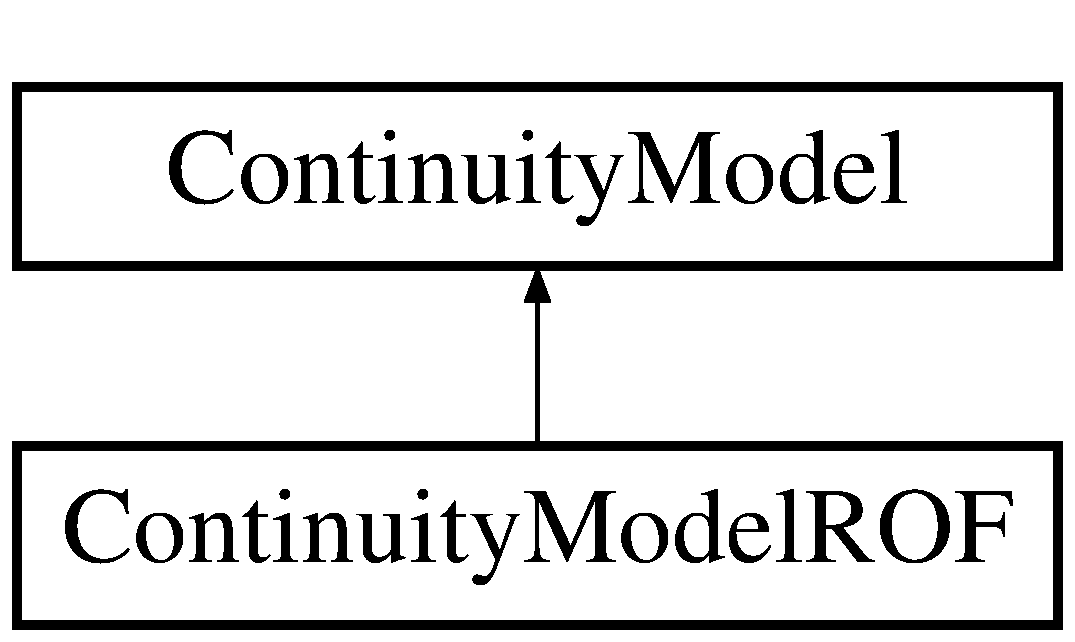
\includegraphics[height=2.000000cm]{classContinuityModelROF}
\end{center}
\end{figure}
\subsection*{Public Member Functions}
\begin{DoxyCompactItemize}
\item 
\mbox{\hyperlink{classContinuityModelROF_a23bd422349e4e2246bd44b2007564fd1}{Continuity\+Model\+R\+OF}} (vector$<$ \mbox{\hyperlink{classWaterSource}{Water\+Source}} $\ast$$>$ water\+\_\+sources, const Graph \&\mbox{\hyperlink{classContinuityModel_a563401588c6fa622f03393909a3522db}{water\+\_\+sources\+\_\+graph}}, const vector$<$ vector$<$ int $>$$>$ \&\mbox{\hyperlink{classContinuityModel_ae8516bcbbf52650190277fc8b06c1843}{water\+\_\+sources\+\_\+to\+\_\+utilities}}, vector$<$ \mbox{\hyperlink{classUtility}{Utility}} $\ast$$>$ utilities, vector$<$ Min\+Env\+Flow\+Control $\ast$$>$ \mbox{\hyperlink{classContinuityModel_afc991e5c0d144020e49a97751a04b302}{min\+\_\+env\+\_\+flow\+\_\+controls}}, vector$<$ double $>$ \&\mbox{\hyperlink{classContinuityModel_aa4a00b76da6295d2faa11e3dcaea1896}{utilities\+\_\+rdm}}, vector$<$ double $>$ \&\mbox{\hyperlink{classContinuityModel_ab7b8fa93a6f56b328e425e1ead6cfefa}{water\+\_\+sources\+\_\+rdm}}, unsigned long total\+\_\+weeks\+\_\+simulation, const int use\+\_\+precomputed\+\_\+rof\+\_\+tables, const unsigned long \mbox{\hyperlink{classContinuityModel_a7b6c99bf256f6c6b633ebb78282f43c7}{realization\+\_\+id}})
\begin{DoxyCompactList}\small\item\em Initializes the \mbox{\hyperlink{classContinuityModelROF}{Continuity\+Model\+R\+OF}} object for simulating risks of failure (R\+OF). \end{DoxyCompactList}\item 
virtual \mbox{\hyperlink{classContinuityModelROF_a4acab850e28a3a41182a19d86a7de709}{$\sim$\+Continuity\+Model\+R\+OF}} ()
\begin{DoxyCompactList}\small\item\em Destructor for the \mbox{\hyperlink{classContinuityModelROF}{Continuity\+Model\+R\+OF}} class. \end{DoxyCompactList}\item 
vector$<$ vector$<$ double $>$ $>$ \mbox{\hyperlink{classContinuityModelROF_a0386963b5914aaaa145de60a2ff1f84e}{calculate\+Short\+Term\+R\+OF}} (int week, int import\+\_\+export\+\_\+rof\+\_\+tables)
\begin{DoxyCompactList}\small\item\em This function calculates the short-\/term risk of failure (R\+OF) for all utilities. \end{DoxyCompactList}\item 
vector$<$ vector$<$ double $>$ $>$ \mbox{\hyperlink{classContinuityModelROF_a975e7566b4c0db6e3731647b6e76b9c8}{calculate\+Short\+Term\+R\+O\+F\+Full\+Calcs}} (int week)
\begin{DoxyCompactList}\small\item\em This function performs a full calculation of the short-\/term risk of failure (R\+OF) for each utility for the given week. \end{DoxyCompactList}\item 
vector$<$ vector$<$ double $>$ $>$ \mbox{\hyperlink{classContinuityModelROF_a48b31e060f1d75e31fa591015f4a1c22}{calculate\+Short\+Term\+R\+O\+F\+Table}} (int week, vector$<$ \mbox{\hyperlink{classUtility}{Utility}} $\ast$$>$ utilities, vector$<$ double $>$ utilities\+\_\+base\+\_\+storage\+\_\+capacity, const vector$<$ Matrix2D$<$ double $>$$>$ \&\mbox{\hyperlink{classContinuityModelROF_ada25d241caf860255ad00097f5e7adb6}{ut\+\_\+storage\+\_\+to\+\_\+rof\+\_\+table}}, vector$<$ double $>$ \mbox{\hyperlink{classContinuityModelROF_a443efa8d5a8bcbb1fea1a0bc929c77cd}{current\+\_\+storage\+\_\+table\+\_\+shift}}, vector$<$ double $>$ \mbox{\hyperlink{classContinuityModelROF_acaebccba4f4ed286c5da02d6c2c90605}{current\+\_\+base\+\_\+storage\+\_\+table\+\_\+shift}}, vector$<$ double $>$ \mbox{\hyperlink{classContinuityModelROF_a1a274033b741e664268515de8e8eb3bc}{current\+\_\+demand\+\_\+ratio\+\_\+buffer}})
\begin{DoxyCompactList}\small\item\em This function calculates the short-\/term risk of failure (R\+OF) for each utility based on the current storage levels and treatment capacity ratios, using a predefined R\+OF table. \end{DoxyCompactList}\item 
vector$<$ vector$<$ double $>$ $>$ \mbox{\hyperlink{classContinuityModelROF_a0b66880fe153cbd0b85a5b416b98e9a6}{calculate\+Long\+Term\+R\+OF}} (int week)
\begin{DoxyCompactList}\small\item\em This function calculates the long-\/term risk of failure (R\+OF) for each utility, considering both storage and treatment capacity, based on projected demand and predefined failure thresholds. \end{DoxyCompactList}\item 
void \mbox{\hyperlink{classContinuityModelROF_acd72d71a29cef49c4de3d111378b76c7}{reset\+Utilities\+And\+Reservoirs}} (int rof\+\_\+type)
\begin{DoxyCompactList}\small\item\em Resets the utilities\textquotesingle{} and reservoirs\textquotesingle{} storage, last release, and combined storage respectively for the specified risk of failure (R\+OF) type. \end{DoxyCompactList}\item 
void \mbox{\hyperlink{classContinuityModelROF_a0c12b5dad97c3783361baad7e53a2634}{connect\+Realization\+Water\+Sources}} (const vector$<$ \mbox{\hyperlink{classWaterSource}{Water\+Source}} $\ast$$>$ \&\mbox{\hyperlink{classContinuityModelROF_a77048d247b8d1f70fbdd31559b4d3337}{realization\+\_\+water\+\_\+sources}})
\begin{DoxyCompactList}\small\item\em Connects this specific realization\textquotesingle{}s water sources to the model by passing the water sources to the R\+OF continuity model for the specific realization it calculated R\+O\+Fs for. \end{DoxyCompactList}\item 
void \mbox{\hyperlink{classContinuityModelROF_abc16c650a854b60dfc42ab2d32ef4b0c}{connect\+Realization\+Utilities}} (const vector$<$ \mbox{\hyperlink{classUtility}{Utility}} $\ast$$>$ \&\mbox{\hyperlink{classContinuityModelROF_a75c6823d8dd37f274ee91ce158088dc4}{realization\+\_\+utilities}})
\begin{DoxyCompactList}\small\item\em Connects the realization utilities to the model by passing in the locations of the utilities of the realization it calculated R\+O\+Fs for. \end{DoxyCompactList}\item 
virtual void \mbox{\hyperlink{classContinuityModelROF_a06cf47a32d6793b0ee912deccf92fc5b}{update\+Online\+Infrastructure}} (int week)
\begin{DoxyCompactList}\small\item\em Updates the online infrastructure for water sources and utilities. \end{DoxyCompactList}\item 
void \mbox{\hyperlink{classContinuityModelROF_a28834584763c3aa27a6f0917aa68926f}{update\+Storage\+To\+R\+O\+F\+Table}} (double storage\+\_\+percent\+\_\+decrement, int week\+\_\+of\+\_\+the\+\_\+year, const double $\ast$to\+\_\+full\+\_\+toposort)
\begin{DoxyCompactList}\small\item\em Updates the approximate storage-\/to-\/\+R\+OF table based on the available water volumes and failure conditions. \end{DoxyCompactList}\item 
void \mbox{\hyperlink{classContinuityModelROF_a4f2b25687bcdeb4a88e22397c84789de}{shift\+Storages}} (double $\ast$available\+\_\+volumes\+\_\+shifted, const double $\ast$delta\+\_\+storage)
\begin{DoxyCompactList}\small\item\em Shifts storage volumes based on delta values. \end{DoxyCompactList}\item 
void \mbox{\hyperlink{classContinuityModelROF_a1bb8362ce39e694937a787805613e106}{print\+R\+O\+F\+Table}} (const string \&folder)
\begin{DoxyCompactList}\small\item\em Prints the R\+OF table to C\+SV files for each utility. \end{DoxyCompactList}\item 
void \mbox{\hyperlink{classContinuityModelROF_a83fc5e19e0f92d12d659c3446b90fa13}{set\+R\+O\+F\+Tables\+And\+Shifts}} (const vector$<$ Matrix2D$<$ double $>$$>$ \&storage\+\_\+to\+\_\+rof\+\_\+table, const vector$<$ vector$<$ double $>$$>$ \&\mbox{\hyperlink{classContinuityModelROF_a1a90c8816944aab36f395e89f7b84c06}{table\+\_\+storage\+\_\+shift}}, const vector$<$ vector$<$ double $>$$>$ \&\mbox{\hyperlink{classContinuityModelROF_a2bc5728653819a0d54a36ffbb1df44a3}{table\+\_\+base\+\_\+storage\+\_\+shift}}, const vector$<$ vector$<$ double $>$$>$ \&\mbox{\hyperlink{classContinuityModelROF_aedb1313e889617d718d2a93d719cb3f1}{treatment\+\_\+demand\+\_\+buffer\+\_\+shift}})
\begin{DoxyCompactList}\small\item\em Sets the R\+OF tables and shifts for the model. \end{DoxyCompactList}\item 
void \mbox{\hyperlink{classContinuityModelROF_a10a8a95f3177d305d3881e654f01d65d}{table\+R\+O\+F\+Exception\+Handler}} (double m, int u, int week)
\begin{DoxyCompactList}\small\item\em Handles exceptions related to R\+OF table extrapolation or errors during R\+OF calculations. \end{DoxyCompactList}\item 
void \mbox{\hyperlink{classContinuityModelROF_a0c46d5905f5d0ae2cf0abd0d4653bbc7}{set\+Initial\+Table\+Tier}} (int week, const int \&utilities, vector$<$ Matrix2D$<$ double $>$$>$ \&vector, int \&tier)
\begin{DoxyCompactList}\small\item\em Sets the initial table tier based on the failure conditions for utilities at a specific week. \end{DoxyCompactList}\item 
void \mbox{\hyperlink{classContinuityModelROF_aa2348a2a5dea751462771ef538243e75}{record\+R\+O\+F\+Storage\+Table}} (vector$<$ Matrix2D$<$ double $>$$>$ \&ut\+\_\+storage\+\_\+to\+\_\+rof\+\_\+rof\+\_\+realization, vector$<$ Matrix2D$<$ double $>$$>$ \&\mbox{\hyperlink{classContinuityModelROF_ada25d241caf860255ad00097f5e7adb6}{ut\+\_\+storage\+\_\+to\+\_\+rof\+\_\+table}}, const int \&\mbox{\hyperlink{classContinuityModel_a6df6198ebc99a099df08f4b8ce6b52b9}{n\+\_\+utilities}}, int \&week, int \&week\+\_\+of\+\_\+the\+\_\+year)
\begin{DoxyCompactList}\small\item\em Records the risk of failure (R\+OF) storage table data for a given utility and week. \end{DoxyCompactList}\item 
void \mbox{\hyperlink{classContinuityModelROF_aa720006d12410fc35b8768eda716c149}{calculate\+Empty\+Volumes}} (vector$<$ \mbox{\hyperlink{classWaterSource}{Water\+Source}} $\ast$$>$ \&\mbox{\hyperlink{classContinuityModelROF_a77048d247b8d1f70fbdd31559b4d3337}{realization\+\_\+water\+\_\+sources}}, double $\ast$to\+\_\+full)
\begin{DoxyCompactList}\small\item\em Calculates the empty volume for each water source. This information is later used for updating the R\+OF tables. \end{DoxyCompactList}\item 
void \mbox{\hyperlink{classContinuityModelROF_a082567cc3a16b971632c14b5a603c692}{update\+Joint\+W\+T\+P\+Treatment\+Allocations}} (const vector$<$ \mbox{\hyperlink{classWaterSource}{Water\+Source}} $\ast$$>$ \&non\+\_\+rof\+\_\+water\+\_\+sources)
\begin{DoxyCompactList}\small\item\em Updates treatment allocations for joint water treatment plants. \end{DoxyCompactList}\item 
void \mbox{\hyperlink{classContinuityModelROF_a360a69a3811c56e8354a64a598228663}{update\+Utility\+Treatment\+Allocations}} (const vector$<$ \mbox{\hyperlink{classUtility}{Utility}} $\ast$$>$ \&non\+\_\+rof\+\_\+utilities)
\begin{DoxyCompactList}\small\item\em Updates treatment capacities for utilities. \end{DoxyCompactList}\item 
vector$<$ Matrix2D$<$ double $>$ $>$ \& \mbox{\hyperlink{classContinuityModelROF_ad798adad5127a2674c5d4a3e8f24302d}{get\+Ut\+\_\+storage\+\_\+to\+\_\+rof\+\_\+table}} ()
\begin{DoxyCompactList}\small\item\em Retrieves the storage-\/to-\/\+R\+OF table. \end{DoxyCompactList}\end{DoxyCompactItemize}
\subsection*{Protected Attributes}
\begin{DoxyCompactItemize}
\item 
int \mbox{\hyperlink{classContinuityModelROF_ad0a8c47eca4ca66b58a2636ab907a4f2}{beginning\+\_\+tier}} = 0
\begin{DoxyCompactList}\small\item\em An integer representing the beginning tier for R\+OF table calculation. \end{DoxyCompactList}\item 
vector$<$ \mbox{\hyperlink{classWaterSource}{Water\+Source}} $\ast$ $>$ \mbox{\hyperlink{classContinuityModelROF_a77048d247b8d1f70fbdd31559b4d3337}{realization\+\_\+water\+\_\+sources}}
\begin{DoxyCompactList}\small\item\em A vector of {\ttfamily \mbox{\hyperlink{classWaterSource}{Water\+Source}}} pointers representing the water sources in the realization. \end{DoxyCompactList}\item 
vector$<$ \mbox{\hyperlink{classUtility}{Utility}} $\ast$ $>$ \mbox{\hyperlink{classContinuityModelROF_a75c6823d8dd37f274ee91ce158088dc4}{realization\+\_\+utilities}}
\begin{DoxyCompactList}\small\item\em A vector of {\ttfamily \mbox{\hyperlink{classUtility}{Utility}}} pointers representing the utilities in the realization. \end{DoxyCompactList}\item 
vector$<$ Matrix2D$<$ double $>$ $>$ \mbox{\hyperlink{classContinuityModelROF_ada25d241caf860255ad00097f5e7adb6}{ut\+\_\+storage\+\_\+to\+\_\+rof\+\_\+table}}
\begin{DoxyCompactList}\small\item\em A vector of {\ttfamily Matrix2D} objects representing the storage-\/to-\/\+R\+OF tables for each utility. \end{DoxyCompactList}\item 
vector$<$ vector$<$ double $>$ $>$ \mbox{\hyperlink{classContinuityModelROF_a1a90c8816944aab36f395e89f7b84c06}{table\+\_\+storage\+\_\+shift}}
\begin{DoxyCompactList}\small\item\em A 2D vector of doubles representing the shifts in storage-\/to-\/\+R\+OF tables for each utility. \end{DoxyCompactList}\item 
vector$<$ vector$<$ double $>$ $>$ \mbox{\hyperlink{classContinuityModelROF_a2bc5728653819a0d54a36ffbb1df44a3}{table\+\_\+base\+\_\+storage\+\_\+shift}}
\begin{DoxyCompactList}\small\item\em A 2D vector of doubles representing the shifts in base storage-\/to-\/\+R\+OF tables for each utility. \end{DoxyCompactList}\item 
vector$<$ vector$<$ double $>$ $>$ \mbox{\hyperlink{classContinuityModelROF_aedb1313e889617d718d2a93d719cb3f1}{treatment\+\_\+demand\+\_\+buffer\+\_\+shift}}
\begin{DoxyCompactList}\small\item\em A 2D vector of doubles representing the shifts in treatment demand buffer for each utility. \end{DoxyCompactList}\item 
vector$<$ double $>$ \mbox{\hyperlink{classContinuityModelROF_a6a429c37f019777325ea4e5b9ad26cae}{utility\+\_\+base\+\_\+storage\+\_\+capacity}}
\begin{DoxyCompactList}\small\item\em A vector of doubles representing the utilities\textquotesingle{} base storage capacities. \end{DoxyCompactList}\item 
vector$<$ double $>$ \mbox{\hyperlink{classContinuityModelROF_a017041335a639ba56cc3e26dea07b514}{utility\+\_\+base\+\_\+delta\+\_\+capacity\+\_\+table}}
\begin{DoxyCompactList}\small\item\em A vector of doubles representing the utilities\textquotesingle{} base delta capacities. \end{DoxyCompactList}\item 
vector$<$ double $>$ \mbox{\hyperlink{classContinuityModelROF_adcaf978b52ba016474952a42856ba373}{current\+\_\+and\+\_\+base\+\_\+storage\+\_\+capacity\+\_\+ratio}}
\begin{DoxyCompactList}\small\item\em A vector of doubles representing the utilities\textquotesingle{} current and base storage capacity ratios. \end{DoxyCompactList}\item 
vector$<$ double $>$ \mbox{\hyperlink{classContinuityModelROF_a443efa8d5a8bcbb1fea1a0bc929c77cd}{current\+\_\+storage\+\_\+table\+\_\+shift}}
\begin{DoxyCompactList}\small\item\em A vector of doubles representing the utilities\textquotesingle{} current storage table shifts. \end{DoxyCompactList}\item 
vector$<$ double $>$ \mbox{\hyperlink{classContinuityModelROF_acaebccba4f4ed286c5da02d6c2c90605}{current\+\_\+base\+\_\+storage\+\_\+table\+\_\+shift}}
\begin{DoxyCompactList}\small\item\em A vector of doubles representing the utilities\textquotesingle{} current base storage table shifts. \end{DoxyCompactList}\item 
vector$<$ double $>$ \mbox{\hyperlink{classContinuityModelROF_a1a274033b741e664268515de8e8eb3bc}{current\+\_\+demand\+\_\+ratio\+\_\+buffer}}
\begin{DoxyCompactList}\small\item\em A vector of doubles representing the utilities\textquotesingle{} current demand ratio buffers. \end{DoxyCompactList}\end{DoxyCompactItemize}
\subsection*{Additional Inherited Members}


\subsection{Constructor \& Destructor Documentation}
\mbox{\Hypertarget{classContinuityModelROF_a23bd422349e4e2246bd44b2007564fd1}\label{classContinuityModelROF_a23bd422349e4e2246bd44b2007564fd1}} 
\index{Continuity\+Model\+R\+OF@{Continuity\+Model\+R\+OF}!Continuity\+Model\+R\+OF@{Continuity\+Model\+R\+OF}}
\index{Continuity\+Model\+R\+OF@{Continuity\+Model\+R\+OF}!Continuity\+Model\+R\+OF@{Continuity\+Model\+R\+OF}}
\subsubsection{\texorpdfstring{Continuity\+Model\+R\+O\+F()}{ContinuityModelROF()}}
{\footnotesize\ttfamily Continuity\+Model\+R\+O\+F\+::\+Continuity\+Model\+R\+OF (\begin{DoxyParamCaption}\item[{vector$<$ \mbox{\hyperlink{classWaterSource}{Water\+Source}} $\ast$$>$}]{water\+\_\+sources,  }\item[{const Graph \&}]{water\+\_\+sources\+\_\+graph,  }\item[{const vector$<$ vector$<$ int $>$$>$ \&}]{water\+\_\+sources\+\_\+to\+\_\+utilities,  }\item[{vector$<$ \mbox{\hyperlink{classUtility}{Utility}} $\ast$$>$}]{utilities,  }\item[{vector$<$ Min\+Env\+Flow\+Control $\ast$$>$}]{min\+\_\+env\+\_\+flow\+\_\+controls,  }\item[{vector$<$ double $>$ \&}]{utilities\+\_\+rdm,  }\item[{vector$<$ double $>$ \&}]{water\+\_\+sources\+\_\+rdm,  }\item[{unsigned long}]{total\+\_\+weeks\+\_\+simulation,  }\item[{const int}]{use\+\_\+precomputed\+\_\+rof\+\_\+tables,  }\item[{const unsigned long}]{realization\+\_\+id }\end{DoxyParamCaption})}



Initializes the \mbox{\hyperlink{classContinuityModelROF}{Continuity\+Model\+R\+OF}} object for simulating risks of failure (R\+OF). 

This constructor sets up the \mbox{\hyperlink{classContinuityModelROF}{Continuity\+Model\+R\+OF}} by initializing storage structures, updating utilities\textquotesingle{} total available volume, and preparing risk-\/of-\/failure (R\+OF) tables or calculations based on pre-\/computed data.


\begin{DoxyParams}{Parameters}
{\em water\+\_\+sources} & Vector of water source objects used in the model. \\
\hline
{\em water\+\_\+sources\+\_\+graph} & Graph representing the topological relationships between water sources. \\
\hline
{\em water\+\_\+sources\+\_\+to\+\_\+utilities} & Mapping of water sources to utilities. \\
\hline
{\em utilities} & Vector of utility objects to manage water demand and allocation. \\
\hline
{\em min\+\_\+env\+\_\+flow\+\_\+controls} & Vector of minimum environmental flow controls. \\
\hline
{\em utilities\+\_\+rdm} & Vector of random deviations for utilities. \\
\hline
{\em water\+\_\+sources\+\_\+rdm} & Vector of random deviations for water sources. \\
\hline
{\em total\+\_\+weeks\+\_\+simulation} & Total number of weeks for the simulation. \\
\hline
{\em use\+\_\+precomputed\+\_\+rof\+\_\+tables} & Indicator for using pre-\/computed R\+OF tables (1\+: use, 0\+: generate dynamically). \\
\hline
{\em realization\+\_\+id} & Unique identifier for the simulation realization. \\
\hline
\end{DoxyParams}
\mbox{\Hypertarget{classContinuityModelROF_a4acab850e28a3a41182a19d86a7de709}\label{classContinuityModelROF_a4acab850e28a3a41182a19d86a7de709}} 
\index{Continuity\+Model\+R\+OF@{Continuity\+Model\+R\+OF}!````~Continuity\+Model\+R\+OF@{$\sim$\+Continuity\+Model\+R\+OF}}
\index{````~Continuity\+Model\+R\+OF@{$\sim$\+Continuity\+Model\+R\+OF}!Continuity\+Model\+R\+OF@{Continuity\+Model\+R\+OF}}
\subsubsection{\texorpdfstring{$\sim$\+Continuity\+Model\+R\+O\+F()}{~ContinuityModelROF()}}
{\footnotesize\ttfamily virtual Continuity\+Model\+R\+O\+F\+::$\sim$\+Continuity\+Model\+R\+OF (\begin{DoxyParamCaption}{ }\end{DoxyParamCaption})\hspace{0.3cm}{\ttfamily [virtual]}}



Destructor for the \mbox{\hyperlink{classContinuityModelROF}{Continuity\+Model\+R\+OF}} class. 

This function cleans up resources allocated during the lifetime of the \mbox{\hyperlink{classContinuityModelROF}{Continuity\+Model\+R\+OF}} object. Specifically, it releases memory associated with dynamically allocated arrays. 

\subsection{Member Function Documentation}
\mbox{\Hypertarget{classContinuityModelROF_aa720006d12410fc35b8768eda716c149}\label{classContinuityModelROF_aa720006d12410fc35b8768eda716c149}} 
\index{Continuity\+Model\+R\+OF@{Continuity\+Model\+R\+OF}!calculate\+Empty\+Volumes@{calculate\+Empty\+Volumes}}
\index{calculate\+Empty\+Volumes@{calculate\+Empty\+Volumes}!Continuity\+Model\+R\+OF@{Continuity\+Model\+R\+OF}}
\subsubsection{\texorpdfstring{calculate\+Empty\+Volumes()}{calculateEmptyVolumes()}}
{\footnotesize\ttfamily void Continuity\+Model\+R\+O\+F\+::calculate\+Empty\+Volumes (\begin{DoxyParamCaption}\item[{vector$<$ \mbox{\hyperlink{classWaterSource}{Water\+Source}} $\ast$$>$ \&}]{realization\+\_\+water\+\_\+sources,  }\item[{double $\ast$}]{to\+\_\+full }\end{DoxyParamCaption})}



Calculates the empty volume for each water source. This information is later used for updating the R\+OF tables. 

This function calculates the empty volume (the volume required to fill a water source to its capacity) for each water source in the {\ttfamily realization\+\_\+water\+\_\+sources} list. The calculation is based on the supply capacity and the available volume for each source. If a water source is offline, the empty volume is set to zero.


\begin{DoxyParams}{Parameters}
{\em realization\+\_\+water\+\_\+sources} & A list of water sources to calculate empty volumes for. \\
\hline
{\em to\+\_\+full} & An array where the empty volume for each water source will be stored.\\
\hline
\end{DoxyParams}
\begin{DoxyReturn}{Returns}
None 
\end{DoxyReturn}
\mbox{\Hypertarget{classContinuityModelROF_a0b66880fe153cbd0b85a5b416b98e9a6}\label{classContinuityModelROF_a0b66880fe153cbd0b85a5b416b98e9a6}} 
\index{Continuity\+Model\+R\+OF@{Continuity\+Model\+R\+OF}!calculate\+Long\+Term\+R\+OF@{calculate\+Long\+Term\+R\+OF}}
\index{calculate\+Long\+Term\+R\+OF@{calculate\+Long\+Term\+R\+OF}!Continuity\+Model\+R\+OF@{Continuity\+Model\+R\+OF}}
\subsubsection{\texorpdfstring{calculate\+Long\+Term\+R\+O\+F()}{calculateLongTermROF()}}
{\footnotesize\ttfamily vector$<$vector$<$double$>$ $>$ Continuity\+Model\+R\+O\+F\+::calculate\+Long\+Term\+R\+OF (\begin{DoxyParamCaption}\item[{int}]{week }\end{DoxyParamCaption})}



This function calculates the long-\/term risk of failure (R\+OF) for each utility, considering both storage and treatment capacity, based on projected demand and predefined failure thresholds. 

The function performs a long-\/term simulation of the utilities\textquotesingle{} storage and treatment capacities over a series of realizations and time steps, calculating the risk of failure for each utility based on storage and treatment conditions.


\begin{DoxyParams}{Parameters}
{\em week} & The current week of the simulation for which the long-\/term R\+OF should be calculated.\\
\hline
\end{DoxyParams}
\begin{DoxyReturn}{Returns}
A 2D vector of doubles representing the risk of failure for each utility\+:
\begin{DoxyItemize}
\item The first row corresponds to the storage-\/related R\+OF.
\item The second row corresponds to the treatment-\/related R\+OF.
\end{DoxyItemize}
\end{DoxyReturn}
\begin{DoxySeeAlso}{See also}
\mbox{\hyperlink{classContinuityModelROF_acd72d71a29cef49c4de3d111378b76c7}{reset\+Utilities\+And\+Reservoirs}}, \mbox{\hyperlink{classContinuityModelROF_a06cf47a32d6793b0ee912deccf92fc5b}{update\+Online\+Infrastructure}} 
\end{DoxySeeAlso}
\mbox{\Hypertarget{classContinuityModelROF_a0386963b5914aaaa145de60a2ff1f84e}\label{classContinuityModelROF_a0386963b5914aaaa145de60a2ff1f84e}} 
\index{Continuity\+Model\+R\+OF@{Continuity\+Model\+R\+OF}!calculate\+Short\+Term\+R\+OF@{calculate\+Short\+Term\+R\+OF}}
\index{calculate\+Short\+Term\+R\+OF@{calculate\+Short\+Term\+R\+OF}!Continuity\+Model\+R\+OF@{Continuity\+Model\+R\+OF}}
\subsubsection{\texorpdfstring{calculate\+Short\+Term\+R\+O\+F()}{calculateShortTermROF()}}
{\footnotesize\ttfamily vector$<$vector$<$double$>$ $>$ Continuity\+Model\+R\+O\+F\+::calculate\+Short\+Term\+R\+OF (\begin{DoxyParamCaption}\item[{int}]{week,  }\item[{int}]{import\+\_\+export\+\_\+rof\+\_\+tables }\end{DoxyParamCaption})}



This function calculates the short-\/term risk of failure (R\+OF) for all utilities. 

Depending on whether precomputed R\+OF tables are imported, the function either performs calculations using the tables or calculates the R\+OF values directly.


\begin{DoxyParams}{Parameters}
{\em week} & The current week in the simulation for which the short-\/term R\+OF is being calculated. \\
\hline
{\em import\+\_\+export\+\_\+rof\+\_\+tables} & Indicator for using precomputed R\+OF tables\+:
\begin{DoxyItemize}
\item I\+M\+P\+O\+R\+T\+\_\+\+R\+O\+F\+\_\+\+T\+A\+B\+L\+ES\+: Use precomputed R\+OF tables.
\item Any other value\+: Perform full calculations for R\+OF.
\end{DoxyItemize}\\
\hline
\end{DoxyParams}
\begin{DoxyReturn}{Returns}
A 2D vector of doubles where each row corresponds to a utility, and columns represent R\+OF values based on different storage or demand conditions. 
\end{DoxyReturn}
\mbox{\Hypertarget{classContinuityModelROF_a975e7566b4c0db6e3731647b6e76b9c8}\label{classContinuityModelROF_a975e7566b4c0db6e3731647b6e76b9c8}} 
\index{Continuity\+Model\+R\+OF@{Continuity\+Model\+R\+OF}!calculate\+Short\+Term\+R\+O\+F\+Full\+Calcs@{calculate\+Short\+Term\+R\+O\+F\+Full\+Calcs}}
\index{calculate\+Short\+Term\+R\+O\+F\+Full\+Calcs@{calculate\+Short\+Term\+R\+O\+F\+Full\+Calcs}!Continuity\+Model\+R\+OF@{Continuity\+Model\+R\+OF}}
\subsubsection{\texorpdfstring{calculate\+Short\+Term\+R\+O\+F\+Full\+Calcs()}{calculateShortTermROFFullCalcs()}}
{\footnotesize\ttfamily vector$<$vector$<$double$>$ $>$ Continuity\+Model\+R\+O\+F\+::calculate\+Short\+Term\+R\+O\+F\+Full\+Calcs (\begin{DoxyParamCaption}\item[{int}]{week }\end{DoxyParamCaption})}



This function performs a full calculation of the short-\/term risk of failure (R\+OF) for each utility for the given week. 

The calculation considers both storage and treatment failure risks over a series of realizations. It simulates the system behavior for multiple years, adjusting for failures based on available storage and treatment capacity.


\begin{DoxyParams}{Parameters}
{\em week} & The current week of the simulation to calculate the short-\/term R\+OF for.\\
\hline
\end{DoxyParams}
\begin{DoxyReturn}{Returns}
A 2D vector of doubles representing the risk of failure for each utility\+:
\begin{DoxyItemize}
\item The first row corresponds to storage-\/related R\+OF.
\item The second row corresponds to treatment-\/related R\+OF.
\end{DoxyItemize}
\end{DoxyReturn}

\begin{DoxyExceptions}{Exceptions}
{\em logic\+\_\+error} & If NaN values are encountered in the R\+OF calculations for storage or treatment.\\
\hline
\end{DoxyExceptions}
\begin{DoxySeeAlso}{See also}
\mbox{\hyperlink{classContinuityModelROF_a28834584763c3aa27a6f0917aa68926f}{update\+Storage\+To\+R\+O\+F\+Table}}, \mbox{\hyperlink{classContinuityModelROF_acd72d71a29cef49c4de3d111378b76c7}{reset\+Utilities\+And\+Reservoirs}}, \mbox{\hyperlink{classContinuityModelROF_a06cf47a32d6793b0ee912deccf92fc5b}{update\+Online\+Infrastructure}}, \mbox{\hyperlink{classContinuityModelROF_a0c46d5905f5d0ae2cf0abd0d4653bbc7}{set\+Initial\+Table\+Tier}}, \mbox{\hyperlink{classContinuityModelROF_aa2348a2a5dea751462771ef538243e75}{record\+R\+O\+F\+Storage\+Table}}, \mbox{\hyperlink{classContinuityModelROF_aa720006d12410fc35b8768eda716c149}{calculate\+Empty\+Volumes}} 
\end{DoxySeeAlso}
\mbox{\Hypertarget{classContinuityModelROF_a48b31e060f1d75e31fa591015f4a1c22}\label{classContinuityModelROF_a48b31e060f1d75e31fa591015f4a1c22}} 
\index{Continuity\+Model\+R\+OF@{Continuity\+Model\+R\+OF}!calculate\+Short\+Term\+R\+O\+F\+Table@{calculate\+Short\+Term\+R\+O\+F\+Table}}
\index{calculate\+Short\+Term\+R\+O\+F\+Table@{calculate\+Short\+Term\+R\+O\+F\+Table}!Continuity\+Model\+R\+OF@{Continuity\+Model\+R\+OF}}
\subsubsection{\texorpdfstring{calculate\+Short\+Term\+R\+O\+F\+Table()}{calculateShortTermROFTable()}}
{\footnotesize\ttfamily vector$<$vector$<$double$>$ $>$ Continuity\+Model\+R\+O\+F\+::calculate\+Short\+Term\+R\+O\+F\+Table (\begin{DoxyParamCaption}\item[{int}]{week,  }\item[{vector$<$ \mbox{\hyperlink{classUtility}{Utility}} $\ast$$>$}]{utilities,  }\item[{vector$<$ double $>$}]{utilities\+\_\+base\+\_\+storage\+\_\+capacity,  }\item[{const vector$<$ Matrix2D$<$ double $>$$>$ \&}]{ut\+\_\+storage\+\_\+to\+\_\+rof\+\_\+table,  }\item[{vector$<$ double $>$}]{current\+\_\+storage\+\_\+table\+\_\+shift,  }\item[{vector$<$ double $>$}]{current\+\_\+base\+\_\+storage\+\_\+table\+\_\+shift,  }\item[{vector$<$ double $>$}]{current\+\_\+demand\+\_\+ratio\+\_\+buffer }\end{DoxyParamCaption})}



This function calculates the short-\/term risk of failure (R\+OF) for each utility based on the current storage levels and treatment capacity ratios, using a predefined R\+OF table. 

The function estimates the risk of failure in both storage and treatment for each utility by comparing the current storage levels against the storage-\/to-\/\+R\+OF table. It also checks if the demand-\/to-\/treatment capacity ratio exceeds a threshold to flag potential treatment failures.


\begin{DoxyParams}{Parameters}
{\em week} & The current week of the simulation for which the short-\/term R\+OF should be calculated. \\
\hline
{\em utilities} & The list of utilities for which the R\+OF will be calculated. \\
\hline
{\em utilities\+\_\+base\+\_\+storage\+\_\+capacity} & The base storage capacities of each utility. \\
\hline
{\em ut\+\_\+storage\+\_\+to\+\_\+rof\+\_\+table} & The precomputed storage-\/to-\/\+R\+OF table for each utility. \\
\hline
{\em current\+\_\+storage\+\_\+table\+\_\+shift} & The current shift applied to the storage table for each utility. \\
\hline
{\em current\+\_\+base\+\_\+storage\+\_\+table\+\_\+shift} & The current shift applied to the base storage table for each utility. \\
\hline
{\em current\+\_\+demand\+\_\+ratio\+\_\+buffer} & The buffer added to the demand-\/to-\/treatment capacity ratio to avoid early failure triggers.\\
\hline
\end{DoxyParams}
\begin{DoxyReturn}{Returns}
A 2D vector of doubles representing the risk of failure for each utility\+:
\begin{DoxyItemize}
\item The first row corresponds to the storage-\/related R\+OF.
\item The second row corresponds to the treatment-\/related R\+OF.
\end{DoxyItemize}
\end{DoxyReturn}
\begin{DoxySeeAlso}{See also}
\mbox{\hyperlink{classContinuityModelROF_a06cf47a32d6793b0ee912deccf92fc5b}{update\+Online\+Infrastructure}} 
\end{DoxySeeAlso}
\mbox{\Hypertarget{classContinuityModelROF_abc16c650a854b60dfc42ab2d32ef4b0c}\label{classContinuityModelROF_abc16c650a854b60dfc42ab2d32ef4b0c}} 
\index{Continuity\+Model\+R\+OF@{Continuity\+Model\+R\+OF}!connect\+Realization\+Utilities@{connect\+Realization\+Utilities}}
\index{connect\+Realization\+Utilities@{connect\+Realization\+Utilities}!Continuity\+Model\+R\+OF@{Continuity\+Model\+R\+OF}}
\subsubsection{\texorpdfstring{connect\+Realization\+Utilities()}{connectRealizationUtilities()}}
{\footnotesize\ttfamily void Continuity\+Model\+R\+O\+F\+::connect\+Realization\+Utilities (\begin{DoxyParamCaption}\item[{const vector$<$ \mbox{\hyperlink{classUtility}{Utility}} $\ast$$>$ \&}]{realization\+\_\+utilities }\end{DoxyParamCaption})}



Connects the realization utilities to the model by passing in the locations of the utilities of the realization it calculated R\+O\+Fs for. 

This function assigns the provided vector of utilities to the realization\textquotesingle{}s utilities. It updates the internal {\ttfamily realization\+\_\+utilities} vector to reflect the current simulation state.


\begin{DoxyParams}{Parameters}
{\em realization\+\_\+utilities} & A vector containing the utilities to be connected to the model.\\
\hline
\end{DoxyParams}
\begin{DoxyReturn}{Returns}
None 
\end{DoxyReturn}
\mbox{\Hypertarget{classContinuityModelROF_a0c12b5dad97c3783361baad7e53a2634}\label{classContinuityModelROF_a0c12b5dad97c3783361baad7e53a2634}} 
\index{Continuity\+Model\+R\+OF@{Continuity\+Model\+R\+OF}!connect\+Realization\+Water\+Sources@{connect\+Realization\+Water\+Sources}}
\index{connect\+Realization\+Water\+Sources@{connect\+Realization\+Water\+Sources}!Continuity\+Model\+R\+OF@{Continuity\+Model\+R\+OF}}
\subsubsection{\texorpdfstring{connect\+Realization\+Water\+Sources()}{connectRealizationWaterSources()}}
{\footnotesize\ttfamily void Continuity\+Model\+R\+O\+F\+::connect\+Realization\+Water\+Sources (\begin{DoxyParamCaption}\item[{const vector$<$ \mbox{\hyperlink{classWaterSource}{Water\+Source}} $\ast$$>$ \&}]{realization\+\_\+water\+\_\+sources }\end{DoxyParamCaption})}



Connects this specific realization\textquotesingle{}s water sources to the model by passing the water sources to the R\+OF continuity model for the specific realization it calculated R\+O\+Fs for. 

This function assigns the provided vector of water sources to the realization\textquotesingle{}s water sources. It updates the internal {\ttfamily realization\+\_\+water\+\_\+sources} vector to reflect the current simulation state.


\begin{DoxyParams}{Parameters}
{\em realization\+\_\+water\+\_\+sources} & A vector containing the one realization\textquotesingle{}s water sources to be connected to the model.\\
\hline
\end{DoxyParams}
\begin{DoxyReturn}{Returns}
None 
\end{DoxyReturn}
\mbox{\Hypertarget{classContinuityModelROF_ad798adad5127a2674c5d4a3e8f24302d}\label{classContinuityModelROF_ad798adad5127a2674c5d4a3e8f24302d}} 
\index{Continuity\+Model\+R\+OF@{Continuity\+Model\+R\+OF}!get\+Ut\+\_\+storage\+\_\+to\+\_\+rof\+\_\+table@{get\+Ut\+\_\+storage\+\_\+to\+\_\+rof\+\_\+table}}
\index{get\+Ut\+\_\+storage\+\_\+to\+\_\+rof\+\_\+table@{get\+Ut\+\_\+storage\+\_\+to\+\_\+rof\+\_\+table}!Continuity\+Model\+R\+OF@{Continuity\+Model\+R\+OF}}
\subsubsection{\texorpdfstring{get\+Ut\+\_\+storage\+\_\+to\+\_\+rof\+\_\+table()}{getUt\_storage\_to\_rof\_table()}}
{\footnotesize\ttfamily vector$<$Matrix2D$<$double$>$ $>$\& Continuity\+Model\+R\+O\+F\+::get\+Ut\+\_\+storage\+\_\+to\+\_\+rof\+\_\+table (\begin{DoxyParamCaption}{ }\end{DoxyParamCaption})}



Retrieves the storage-\/to-\/\+R\+OF table. 

This function returns a reference to the storage-\/to-\/\+R\+OF table, which contains the calculated risk of failure (R\+OF) for each utility at various storage levels.


\begin{DoxyParams}{Parameters}
{\em None} & \\
\hline
\end{DoxyParams}
\begin{DoxyReturn}{Returns}
A reference to the storage-\/to-\/\+R\+OF table ({\ttfamily ut\+\_\+storage\+\_\+to\+\_\+rof\+\_\+table}). 
\end{DoxyReturn}
\mbox{\Hypertarget{classContinuityModelROF_a1bb8362ce39e694937a787805613e106}\label{classContinuityModelROF_a1bb8362ce39e694937a787805613e106}} 
\index{Continuity\+Model\+R\+OF@{Continuity\+Model\+R\+OF}!print\+R\+O\+F\+Table@{print\+R\+O\+F\+Table}}
\index{print\+R\+O\+F\+Table@{print\+R\+O\+F\+Table}!Continuity\+Model\+R\+OF@{Continuity\+Model\+R\+OF}}
\subsubsection{\texorpdfstring{print\+R\+O\+F\+Table()}{printROFTable()}}
{\footnotesize\ttfamily void Continuity\+Model\+R\+O\+F\+::print\+R\+O\+F\+Table (\begin{DoxyParamCaption}\item[{const string \&}]{folder }\end{DoxyParamCaption})}



Prints the R\+OF table to C\+SV files for each utility. 

F\+I\+X\+ME\+: This is where changes from C\+SV to more efficient file formats should be made.

This function generates C\+SV files containing the Risk of Failure (R\+OF) data for each utility. It iterates over the number of utilities and writes the R\+OF table data to a separate file for each utility. The files are saved in the specified folder with filenames indicating the realization ID and the utility index.


\begin{DoxyParams}{Parameters}
{\em folder} & The folder path where the C\+SV files will be saved.\\
\hline
\end{DoxyParams}
\begin{DoxyReturn}{Returns}
None 
\end{DoxyReturn}
\mbox{\Hypertarget{classContinuityModelROF_aa2348a2a5dea751462771ef538243e75}\label{classContinuityModelROF_aa2348a2a5dea751462771ef538243e75}} 
\index{Continuity\+Model\+R\+OF@{Continuity\+Model\+R\+OF}!record\+R\+O\+F\+Storage\+Table@{record\+R\+O\+F\+Storage\+Table}}
\index{record\+R\+O\+F\+Storage\+Table@{record\+R\+O\+F\+Storage\+Table}!Continuity\+Model\+R\+OF@{Continuity\+Model\+R\+OF}}
\subsubsection{\texorpdfstring{record\+R\+O\+F\+Storage\+Table()}{recordROFStorageTable()}}
{\footnotesize\ttfamily void Continuity\+Model\+R\+O\+F\+::record\+R\+O\+F\+Storage\+Table (\begin{DoxyParamCaption}\item[{vector$<$ Matrix2D$<$ double $>$$>$ \&}]{ut\+\_\+storage\+\_\+to\+\_\+rof\+\_\+rof\+\_\+realization,  }\item[{vector$<$ Matrix2D$<$ double $>$$>$ \&}]{ut\+\_\+storage\+\_\+to\+\_\+rof\+\_\+table,  }\item[{const int \&}]{n\+\_\+utilities,  }\item[{int \&}]{week,  }\item[{int \&}]{week\+\_\+of\+\_\+the\+\_\+year }\end{DoxyParamCaption})}



Records the risk of failure (R\+OF) storage table data for a given utility and week. 

This function updates the {\ttfamily ut\+\_\+storage\+\_\+to\+\_\+rof\+\_\+table} by adding R\+OF data for each utility at the specified week. The R\+OF data is retrieved from the corresponding realization table, averaged over all realizations, and then added to the storage table for that week.


\begin{DoxyParams}{Parameters}
{\em ut\+\_\+storage\+\_\+to\+\_\+rof\+\_\+rof\+\_\+realization} & The R\+OF data for all utilities across multiple realizations. \\
\hline
{\em ut\+\_\+storage\+\_\+to\+\_\+rof\+\_\+table} & The storage to R\+OF table to which the data is to be added. \\
\hline
{\em n\+\_\+utilities} & The number of utilities being considered. \\
\hline
{\em week} & The current week in the simulation. \\
\hline
{\em week\+\_\+of\+\_\+the\+\_\+year} & The specific week of the year to record data for.\\
\hline
\end{DoxyParams}
\begin{DoxyReturn}{Returns}
None 
\end{DoxyReturn}
\mbox{\Hypertarget{classContinuityModelROF_acd72d71a29cef49c4de3d111378b76c7}\label{classContinuityModelROF_acd72d71a29cef49c4de3d111378b76c7}} 
\index{Continuity\+Model\+R\+OF@{Continuity\+Model\+R\+OF}!reset\+Utilities\+And\+Reservoirs@{reset\+Utilities\+And\+Reservoirs}}
\index{reset\+Utilities\+And\+Reservoirs@{reset\+Utilities\+And\+Reservoirs}!Continuity\+Model\+R\+OF@{Continuity\+Model\+R\+OF}}
\subsubsection{\texorpdfstring{reset\+Utilities\+And\+Reservoirs()}{resetUtilitiesAndReservoirs()}}
{\footnotesize\ttfamily void Continuity\+Model\+R\+O\+F\+::reset\+Utilities\+And\+Reservoirs (\begin{DoxyParamCaption}\item[{int}]{rof\+\_\+type }\end{DoxyParamCaption})}



Resets the utilities\textquotesingle{} and reservoirs\textquotesingle{} storage, last release, and combined storage respectively for the specified risk of failure (R\+OF) type. 

This function updates the water sources\textquotesingle{} available volumes and outflows based on the current R\+OF type (short-\/term or long-\/term). It also updates the total available volume for each utility.


\begin{DoxyParams}{Parameters}
{\em rof\+\_\+type} & The type of R\+OF being simulated. Can be either\+:
\begin{DoxyItemize}
\item {\ttfamily S\+H\+O\+R\+T\+\_\+\+T\+E\+R\+M\+\_\+\+R\+OF}\+: For resetting to current storage conditions.
\item {\ttfamily L\+O\+N\+G\+\_\+\+T\+E\+R\+M\+\_\+\+R\+OF}\+: For resetting to full capacity conditions.
\end{DoxyItemize}\\
\hline
\end{DoxyParams}
\begin{DoxyReturn}{Returns}
None 
\end{DoxyReturn}
\mbox{\Hypertarget{classContinuityModelROF_a0c46d5905f5d0ae2cf0abd0d4653bbc7}\label{classContinuityModelROF_a0c46d5905f5d0ae2cf0abd0d4653bbc7}} 
\index{Continuity\+Model\+R\+OF@{Continuity\+Model\+R\+OF}!set\+Initial\+Table\+Tier@{set\+Initial\+Table\+Tier}}
\index{set\+Initial\+Table\+Tier@{set\+Initial\+Table\+Tier}!Continuity\+Model\+R\+OF@{Continuity\+Model\+R\+OF}}
\subsubsection{\texorpdfstring{set\+Initial\+Table\+Tier()}{setInitialTableTier()}}
{\footnotesize\ttfamily void Continuity\+Model\+R\+O\+F\+::set\+Initial\+Table\+Tier (\begin{DoxyParamCaption}\item[{int}]{week,  }\item[{const int \&}]{utilities,  }\item[{vector$<$ Matrix2D$<$ double $>$$>$ \&}]{vector,  }\item[{int \&}]{tier }\end{DoxyParamCaption})}



Sets the initial table tier based on the failure conditions for utilities at a specific week. 

This function determines the initial table tier by checking for failures across utilities and adjusting the tier accordingly. It searches through the storage to R\+OF table and identifies the first tier where no failures occurred, setting that as the beginning tier for the simulation.


\begin{DoxyParams}{Parameters}
{\em week} & The current week in the simulation. \\
\hline
{\em n\+\_\+utilities} & The number of utilities to be considered in the table. \\
\hline
{\em ut\+\_\+storage\+\_\+to\+\_\+rof\+\_\+table} & The table containing storage to R\+OF data for utilities. \\
\hline
{\em beginning\+\_\+tier} & The tier to be set as the starting point for the calculations.\\
\hline
\end{DoxyParams}
\begin{DoxyReturn}{Returns}
None 
\end{DoxyReturn}
\mbox{\Hypertarget{classContinuityModelROF_a83fc5e19e0f92d12d659c3446b90fa13}\label{classContinuityModelROF_a83fc5e19e0f92d12d659c3446b90fa13}} 
\index{Continuity\+Model\+R\+OF@{Continuity\+Model\+R\+OF}!set\+R\+O\+F\+Tables\+And\+Shifts@{set\+R\+O\+F\+Tables\+And\+Shifts}}
\index{set\+R\+O\+F\+Tables\+And\+Shifts@{set\+R\+O\+F\+Tables\+And\+Shifts}!Continuity\+Model\+R\+OF@{Continuity\+Model\+R\+OF}}
\subsubsection{\texorpdfstring{set\+R\+O\+F\+Tables\+And\+Shifts()}{setROFTablesAndShifts()}}
{\footnotesize\ttfamily void Continuity\+Model\+R\+O\+F\+::set\+R\+O\+F\+Tables\+And\+Shifts (\begin{DoxyParamCaption}\item[{const vector$<$ Matrix2D$<$ double $>$$>$ \&}]{storage\+\_\+to\+\_\+rof\+\_\+table,  }\item[{const vector$<$ vector$<$ double $>$$>$ \&}]{table\+\_\+storage\+\_\+shift,  }\item[{const vector$<$ vector$<$ double $>$$>$ \&}]{table\+\_\+base\+\_\+storage\+\_\+shift,  }\item[{const vector$<$ vector$<$ double $>$$>$ \&}]{treatment\+\_\+demand\+\_\+buffer\+\_\+shift }\end{DoxyParamCaption})}



Sets the R\+OF tables and shifts for the model. 

This function assigns the provided R\+OF tables and related shift data to the corresponding member variables in the model. The shift data is used for adjusting the storage and demand conditions during the R\+OF calculation processes.


\begin{DoxyParams}{Parameters}
{\em storage\+\_\+to\+\_\+rof\+\_\+table} & The 2D matrix of storage-\/to-\/\+R\+OF data. \\
\hline
{\em table\+\_\+storage\+\_\+shift} & The shift values for the storage table. \\
\hline
{\em table\+\_\+base\+\_\+storage\+\_\+shift} & The shift values for the base storage table. \\
\hline
{\em treatment\+\_\+demand\+\_\+buffer\+\_\+shift} & The shift values for the treatment demand buffer.\\
\hline
\end{DoxyParams}
\begin{DoxyReturn}{Returns}
None 
\end{DoxyReturn}
\mbox{\Hypertarget{classContinuityModelROF_a4f2b25687bcdeb4a88e22397c84789de}\label{classContinuityModelROF_a4f2b25687bcdeb4a88e22397c84789de}} 
\index{Continuity\+Model\+R\+OF@{Continuity\+Model\+R\+OF}!shift\+Storages@{shift\+Storages}}
\index{shift\+Storages@{shift\+Storages}!Continuity\+Model\+R\+OF@{Continuity\+Model\+R\+OF}}
\subsubsection{\texorpdfstring{shift\+Storages()}{shiftStorages()}}
{\footnotesize\ttfamily void Continuity\+Model\+R\+O\+F\+::shift\+Storages (\begin{DoxyParamCaption}\item[{double $\ast$}]{available\+\_\+volumes\+\_\+shifted,  }\item[{const double $\ast$}]{delta\+\_\+storage }\end{DoxyParamCaption})}



Shifts storage volumes based on delta values. 

This function adjusts the storage volumes of water sources according to the given delta values. It handles the spillover of water to downstream sources if a source\textquotesingle{}s storage exceeds its capacity. The function is designed to respect the topological order of sources, ensuring that upstream sources are processed before downstream sources.

F\+I\+X\+ME\+: M\+A\+KE T\+H\+IS M\+O\+RE E\+F\+F\+I\+C\+I\+E\+NT. T\+H\+IS M\+E\+T\+H\+OD IS T\+HE M\+O\+ST E\+X\+P\+E\+N\+S\+I\+VE O\+NE IN T\+HE C\+O\+DE.


\begin{DoxyParams}{Parameters}
{\em available\+\_\+volumes\+\_\+shifted} & A pointer to an array representing the shifted available volumes for each water source. \\
\hline
{\em delta\+\_\+storage} & A pointer to an array of delta values representing the change in storage for each water source.\\
\hline
\end{DoxyParams}
\begin{DoxyReturn}{Returns}
None 
\end{DoxyReturn}
\mbox{\Hypertarget{classContinuityModelROF_a10a8a95f3177d305d3881e654f01d65d}\label{classContinuityModelROF_a10a8a95f3177d305d3881e654f01d65d}} 
\index{Continuity\+Model\+R\+OF@{Continuity\+Model\+R\+OF}!table\+R\+O\+F\+Exception\+Handler@{table\+R\+O\+F\+Exception\+Handler}}
\index{table\+R\+O\+F\+Exception\+Handler@{table\+R\+O\+F\+Exception\+Handler}!Continuity\+Model\+R\+OF@{Continuity\+Model\+R\+OF}}
\subsubsection{\texorpdfstring{table\+R\+O\+F\+Exception\+Handler()}{tableROFExceptionHandler()}}
{\footnotesize\ttfamily void Continuity\+Model\+R\+O\+F\+::table\+R\+O\+F\+Exception\+Handler (\begin{DoxyParamCaption}\item[{double}]{m,  }\item[{int}]{u,  }\item[{int}]{week }\end{DoxyParamCaption})}



Handles exceptions related to R\+OF table extrapolation or errors during R\+OF calculations. 

This function throws an exception if the R\+OF tables need to be extrapolated due to a utility\textquotesingle{}s current capacity exceeding the table\textquotesingle{}s base capacity. If the error is related to table extrapolation, it provides guidance to regenerate tables with adjusted parameters. If the error occurs in a different context, a runtime exception is thrown with the appropriate details.


\begin{DoxyParams}{Parameters}
{\em m} & The ratio of current storage capacity to the base storage capacity. \\
\hline
{\em u} & The index of the utility where the exception occurred. \\
\hline
{\em week} & The current week in the simulation where the error occurred.\\
\hline
\end{DoxyParams}
\begin{DoxyReturn}{Returns}
None
\end{DoxyReturn}

\begin{DoxyExceptions}{Exceptions}
{\em logic\+\_\+error} & If {\ttfamily m} is greater than 1, indicating that the current capacity is greater than the table base capacity. \\
\hline
{\em runtime\+\_\+error} & For other exceptions that occur within a specific week for a utility. \\
\hline
\end{DoxyExceptions}
\mbox{\Hypertarget{classContinuityModelROF_a082567cc3a16b971632c14b5a603c692}\label{classContinuityModelROF_a082567cc3a16b971632c14b5a603c692}} 
\index{Continuity\+Model\+R\+OF@{Continuity\+Model\+R\+OF}!update\+Joint\+W\+T\+P\+Treatment\+Allocations@{update\+Joint\+W\+T\+P\+Treatment\+Allocations}}
\index{update\+Joint\+W\+T\+P\+Treatment\+Allocations@{update\+Joint\+W\+T\+P\+Treatment\+Allocations}!Continuity\+Model\+R\+OF@{Continuity\+Model\+R\+OF}}
\subsubsection{\texorpdfstring{update\+Joint\+W\+T\+P\+Treatment\+Allocations()}{updateJointWTPTreatmentAllocations()}}
{\footnotesize\ttfamily void Continuity\+Model\+R\+O\+F\+::update\+Joint\+W\+T\+P\+Treatment\+Allocations (\begin{DoxyParamCaption}\item[{const vector$<$ \mbox{\hyperlink{classWaterSource}{Water\+Source}} $\ast$$>$ \&}]{non\+\_\+rof\+\_\+water\+\_\+sources }\end{DoxyParamCaption})}



Updates treatment allocations for joint water treatment plants. 

This function updates the treatment allocations for water sources of type {\ttfamily N\+E\+W\+\_\+\+J\+O\+I\+N\+T\+\_\+\+W\+A\+T\+E\+R\+\_\+\+T\+R\+E\+A\+T\+M\+E\+N\+T\+\_\+\+P\+L\+A\+NT} in the {\ttfamily non\+\_\+rof\+\_\+water\+\_\+sources} list. It ensures that the treatment allocations are synchronized between the continuity and realization water sources if the source is online.

F\+I\+X\+ME\+: W\+H\+AT IS T\+HE F\+U\+N\+C\+T\+I\+O\+N\+AL D\+I\+F\+F\+E\+R\+E\+N\+CE B\+E\+T\+W\+E\+EN W\+A\+T\+E\+R\+\_\+\+S\+O\+U\+R\+C\+ES V\+E\+C\+T\+O\+RS H\+E\+RE?


\begin{DoxyParams}{Parameters}
{\em non\+\_\+rof\+\_\+water\+\_\+sources} & A list of non-\/\+R\+OF water sources whose treatment allocations will be updated.\\
\hline
\end{DoxyParams}
\begin{DoxyReturn}{Returns}
None 
\end{DoxyReturn}
\mbox{\Hypertarget{classContinuityModelROF_a06cf47a32d6793b0ee912deccf92fc5b}\label{classContinuityModelROF_a06cf47a32d6793b0ee912deccf92fc5b}} 
\index{Continuity\+Model\+R\+OF@{Continuity\+Model\+R\+OF}!update\+Online\+Infrastructure@{update\+Online\+Infrastructure}}
\index{update\+Online\+Infrastructure@{update\+Online\+Infrastructure}!Continuity\+Model\+R\+OF@{Continuity\+Model\+R\+OF}}
\subsubsection{\texorpdfstring{update\+Online\+Infrastructure()}{updateOnlineInfrastructure()}}
{\footnotesize\ttfamily virtual void Continuity\+Model\+R\+O\+F\+::update\+Online\+Infrastructure (\begin{DoxyParamCaption}\item[{int}]{week }\end{DoxyParamCaption})\hspace{0.3cm}{\ttfamily [virtual]}}



Updates the online infrastructure for water sources and utilities. 

This function checks for any new infrastructure that has become online in the realization model and updates the corresponding infrastructure status in the continuity model (R\+OF model). It updates water sources\textquotesingle{} capacities, utilities\textquotesingle{} storage capacities, and their ratios to status-\/quo capacities. It also updates the list of downstream sources for each source.


\begin{DoxyParams}{Parameters}
{\em week} & The current week number for the simulation.\\
\hline
\end{DoxyParams}
\begin{DoxyReturn}{Returns}
None 
\end{DoxyReturn}
\mbox{\Hypertarget{classContinuityModelROF_a28834584763c3aa27a6f0917aa68926f}\label{classContinuityModelROF_a28834584763c3aa27a6f0917aa68926f}} 
\index{Continuity\+Model\+R\+OF@{Continuity\+Model\+R\+OF}!update\+Storage\+To\+R\+O\+F\+Table@{update\+Storage\+To\+R\+O\+F\+Table}}
\index{update\+Storage\+To\+R\+O\+F\+Table@{update\+Storage\+To\+R\+O\+F\+Table}!Continuity\+Model\+R\+OF@{Continuity\+Model\+R\+OF}}
\subsubsection{\texorpdfstring{update\+Storage\+To\+R\+O\+F\+Table()}{updateStorageToROFTable()}}
{\footnotesize\ttfamily void Continuity\+Model\+R\+O\+F\+::update\+Storage\+To\+R\+O\+F\+Table (\begin{DoxyParamCaption}\item[{double}]{storage\+\_\+percent\+\_\+decrement,  }\item[{int}]{week\+\_\+of\+\_\+the\+\_\+year,  }\item[{const double $\ast$}]{to\+\_\+full\+\_\+toposort }\end{DoxyParamCaption})}



Updates the approximate storage-\/to-\/\+R\+OF table based on the available water volumes and failure conditions. 

This function updates the storage-\/to-\/\+R\+OF table for each week by shifting storage volumes and checking for utility failures at various storage levels. The function reduces storage levels incrementally and records failures for utilities that do not meet the required storage capacity ratio. The process stops once all utilities have failed at a particular storage level.


\begin{DoxyParams}{Parameters}
{\em storage\+\_\+percent\+\_\+decrement} & The percentage decrement to apply to the storage levels. \\
\hline
{\em week\+\_\+of\+\_\+the\+\_\+year} & The week of the year to update the table for. \\
\hline
{\em to\+\_\+full} & Array of available water volumes to full storage capacity for each water source.\\
\hline
\end{DoxyParams}
\begin{DoxyReturn}{Returns}
None
\end{DoxyReturn}
\begin{DoxySeeAlso}{See also}
\mbox{\hyperlink{classContinuityModelROF_a4f2b25687bcdeb4a88e22397c84789de}{shift\+Storages}} 
\end{DoxySeeAlso}
\mbox{\Hypertarget{classContinuityModelROF_a360a69a3811c56e8354a64a598228663}\label{classContinuityModelROF_a360a69a3811c56e8354a64a598228663}} 
\index{Continuity\+Model\+R\+OF@{Continuity\+Model\+R\+OF}!update\+Utility\+Treatment\+Allocations@{update\+Utility\+Treatment\+Allocations}}
\index{update\+Utility\+Treatment\+Allocations@{update\+Utility\+Treatment\+Allocations}!Continuity\+Model\+R\+OF@{Continuity\+Model\+R\+OF}}
\subsubsection{\texorpdfstring{update\+Utility\+Treatment\+Allocations()}{updateUtilityTreatmentAllocations()}}
{\footnotesize\ttfamily void Continuity\+Model\+R\+O\+F\+::update\+Utility\+Treatment\+Allocations (\begin{DoxyParamCaption}\item[{const vector$<$ \mbox{\hyperlink{classUtility}{Utility}} $\ast$$>$ \&}]{non\+\_\+rof\+\_\+utilities }\end{DoxyParamCaption})}



Updates treatment capacities for utilities. 

This function updates the treatment capacities for utilities in the {\ttfamily non\+\_\+rof\+\_\+utilities} list by synchronizing the treatment capacities between the continuity and realization utilities.

F\+I\+X\+ME\+: W\+H\+AT IS T\+HE F\+U\+N\+C\+T\+I\+O\+N\+AL D\+I\+F\+F\+E\+R\+E\+N\+CE B\+E\+T\+W\+E\+EN W\+A\+T\+E\+R\+\_\+\+S\+O\+U\+R\+C\+ES V\+E\+C\+T\+O\+RS H\+E\+RE?


\begin{DoxyParams}{Parameters}
{\em non\+\_\+rof\+\_\+utilities} & A list of non-\/\+R\+OF utilities whose treatment capacities will be updated.\\
\hline
\end{DoxyParams}
\begin{DoxyReturn}{Returns}
None 
\end{DoxyReturn}


\subsection{Member Data Documentation}
\mbox{\Hypertarget{classContinuityModelROF_ad0a8c47eca4ca66b58a2636ab907a4f2}\label{classContinuityModelROF_ad0a8c47eca4ca66b58a2636ab907a4f2}} 
\index{Continuity\+Model\+R\+OF@{Continuity\+Model\+R\+OF}!beginning\+\_\+tier@{beginning\+\_\+tier}}
\index{beginning\+\_\+tier@{beginning\+\_\+tier}!Continuity\+Model\+R\+OF@{Continuity\+Model\+R\+OF}}
\subsubsection{\texorpdfstring{beginning\+\_\+tier}{beginning\_tier}}
{\footnotesize\ttfamily int Continuity\+Model\+R\+O\+F\+::beginning\+\_\+tier = 0\hspace{0.3cm}{\ttfamily [protected]}}



An integer representing the beginning tier for R\+OF table calculation. 

\mbox{\Hypertarget{classContinuityModelROF_adcaf978b52ba016474952a42856ba373}\label{classContinuityModelROF_adcaf978b52ba016474952a42856ba373}} 
\index{Continuity\+Model\+R\+OF@{Continuity\+Model\+R\+OF}!current\+\_\+and\+\_\+base\+\_\+storage\+\_\+capacity\+\_\+ratio@{current\+\_\+and\+\_\+base\+\_\+storage\+\_\+capacity\+\_\+ratio}}
\index{current\+\_\+and\+\_\+base\+\_\+storage\+\_\+capacity\+\_\+ratio@{current\+\_\+and\+\_\+base\+\_\+storage\+\_\+capacity\+\_\+ratio}!Continuity\+Model\+R\+OF@{Continuity\+Model\+R\+OF}}
\subsubsection{\texorpdfstring{current\+\_\+and\+\_\+base\+\_\+storage\+\_\+capacity\+\_\+ratio}{current\_and\_base\_storage\_capacity\_ratio}}
{\footnotesize\ttfamily vector$<$double$>$ Continuity\+Model\+R\+O\+F\+::current\+\_\+and\+\_\+base\+\_\+storage\+\_\+capacity\+\_\+ratio\hspace{0.3cm}{\ttfamily [protected]}}



A vector of doubles representing the utilities\textquotesingle{} current and base storage capacity ratios. 

\mbox{\Hypertarget{classContinuityModelROF_acaebccba4f4ed286c5da02d6c2c90605}\label{classContinuityModelROF_acaebccba4f4ed286c5da02d6c2c90605}} 
\index{Continuity\+Model\+R\+OF@{Continuity\+Model\+R\+OF}!current\+\_\+base\+\_\+storage\+\_\+table\+\_\+shift@{current\+\_\+base\+\_\+storage\+\_\+table\+\_\+shift}}
\index{current\+\_\+base\+\_\+storage\+\_\+table\+\_\+shift@{current\+\_\+base\+\_\+storage\+\_\+table\+\_\+shift}!Continuity\+Model\+R\+OF@{Continuity\+Model\+R\+OF}}
\subsubsection{\texorpdfstring{current\+\_\+base\+\_\+storage\+\_\+table\+\_\+shift}{current\_base\_storage\_table\_shift}}
{\footnotesize\ttfamily vector$<$double$>$ Continuity\+Model\+R\+O\+F\+::current\+\_\+base\+\_\+storage\+\_\+table\+\_\+shift\hspace{0.3cm}{\ttfamily [protected]}}



A vector of doubles representing the utilities\textquotesingle{} current base storage table shifts. 

\mbox{\Hypertarget{classContinuityModelROF_a1a274033b741e664268515de8e8eb3bc}\label{classContinuityModelROF_a1a274033b741e664268515de8e8eb3bc}} 
\index{Continuity\+Model\+R\+OF@{Continuity\+Model\+R\+OF}!current\+\_\+demand\+\_\+ratio\+\_\+buffer@{current\+\_\+demand\+\_\+ratio\+\_\+buffer}}
\index{current\+\_\+demand\+\_\+ratio\+\_\+buffer@{current\+\_\+demand\+\_\+ratio\+\_\+buffer}!Continuity\+Model\+R\+OF@{Continuity\+Model\+R\+OF}}
\subsubsection{\texorpdfstring{current\+\_\+demand\+\_\+ratio\+\_\+buffer}{current\_demand\_ratio\_buffer}}
{\footnotesize\ttfamily vector$<$double$>$ Continuity\+Model\+R\+O\+F\+::current\+\_\+demand\+\_\+ratio\+\_\+buffer\hspace{0.3cm}{\ttfamily [protected]}}



A vector of doubles representing the utilities\textquotesingle{} current demand ratio buffers. 

\mbox{\Hypertarget{classContinuityModelROF_a443efa8d5a8bcbb1fea1a0bc929c77cd}\label{classContinuityModelROF_a443efa8d5a8bcbb1fea1a0bc929c77cd}} 
\index{Continuity\+Model\+R\+OF@{Continuity\+Model\+R\+OF}!current\+\_\+storage\+\_\+table\+\_\+shift@{current\+\_\+storage\+\_\+table\+\_\+shift}}
\index{current\+\_\+storage\+\_\+table\+\_\+shift@{current\+\_\+storage\+\_\+table\+\_\+shift}!Continuity\+Model\+R\+OF@{Continuity\+Model\+R\+OF}}
\subsubsection{\texorpdfstring{current\+\_\+storage\+\_\+table\+\_\+shift}{current\_storage\_table\_shift}}
{\footnotesize\ttfamily vector$<$double$>$ Continuity\+Model\+R\+O\+F\+::current\+\_\+storage\+\_\+table\+\_\+shift\hspace{0.3cm}{\ttfamily [protected]}}



A vector of doubles representing the utilities\textquotesingle{} current storage table shifts. 

\mbox{\Hypertarget{classContinuityModelROF_a75c6823d8dd37f274ee91ce158088dc4}\label{classContinuityModelROF_a75c6823d8dd37f274ee91ce158088dc4}} 
\index{Continuity\+Model\+R\+OF@{Continuity\+Model\+R\+OF}!realization\+\_\+utilities@{realization\+\_\+utilities}}
\index{realization\+\_\+utilities@{realization\+\_\+utilities}!Continuity\+Model\+R\+OF@{Continuity\+Model\+R\+OF}}
\subsubsection{\texorpdfstring{realization\+\_\+utilities}{realization\_utilities}}
{\footnotesize\ttfamily vector$<$\mbox{\hyperlink{classUtility}{Utility}} $\ast$$>$ Continuity\+Model\+R\+O\+F\+::realization\+\_\+utilities\hspace{0.3cm}{\ttfamily [protected]}}



A vector of {\ttfamily \mbox{\hyperlink{classUtility}{Utility}}} pointers representing the utilities in the realization. 

\mbox{\Hypertarget{classContinuityModelROF_a77048d247b8d1f70fbdd31559b4d3337}\label{classContinuityModelROF_a77048d247b8d1f70fbdd31559b4d3337}} 
\index{Continuity\+Model\+R\+OF@{Continuity\+Model\+R\+OF}!realization\+\_\+water\+\_\+sources@{realization\+\_\+water\+\_\+sources}}
\index{realization\+\_\+water\+\_\+sources@{realization\+\_\+water\+\_\+sources}!Continuity\+Model\+R\+OF@{Continuity\+Model\+R\+OF}}
\subsubsection{\texorpdfstring{realization\+\_\+water\+\_\+sources}{realization\_water\_sources}}
{\footnotesize\ttfamily vector$<$\mbox{\hyperlink{classWaterSource}{Water\+Source}} $\ast$$>$ Continuity\+Model\+R\+O\+F\+::realization\+\_\+water\+\_\+sources\hspace{0.3cm}{\ttfamily [protected]}}



A vector of {\ttfamily \mbox{\hyperlink{classWaterSource}{Water\+Source}}} pointers representing the water sources in the realization. 

\mbox{\Hypertarget{classContinuityModelROF_a2bc5728653819a0d54a36ffbb1df44a3}\label{classContinuityModelROF_a2bc5728653819a0d54a36ffbb1df44a3}} 
\index{Continuity\+Model\+R\+OF@{Continuity\+Model\+R\+OF}!table\+\_\+base\+\_\+storage\+\_\+shift@{table\+\_\+base\+\_\+storage\+\_\+shift}}
\index{table\+\_\+base\+\_\+storage\+\_\+shift@{table\+\_\+base\+\_\+storage\+\_\+shift}!Continuity\+Model\+R\+OF@{Continuity\+Model\+R\+OF}}
\subsubsection{\texorpdfstring{table\+\_\+base\+\_\+storage\+\_\+shift}{table\_base\_storage\_shift}}
{\footnotesize\ttfamily vector$<$vector$<$double$>$ $>$ Continuity\+Model\+R\+O\+F\+::table\+\_\+base\+\_\+storage\+\_\+shift\hspace{0.3cm}{\ttfamily [protected]}}



A 2D vector of doubles representing the shifts in base storage-\/to-\/\+R\+OF tables for each utility. 

\mbox{\Hypertarget{classContinuityModelROF_a1a90c8816944aab36f395e89f7b84c06}\label{classContinuityModelROF_a1a90c8816944aab36f395e89f7b84c06}} 
\index{Continuity\+Model\+R\+OF@{Continuity\+Model\+R\+OF}!table\+\_\+storage\+\_\+shift@{table\+\_\+storage\+\_\+shift}}
\index{table\+\_\+storage\+\_\+shift@{table\+\_\+storage\+\_\+shift}!Continuity\+Model\+R\+OF@{Continuity\+Model\+R\+OF}}
\subsubsection{\texorpdfstring{table\+\_\+storage\+\_\+shift}{table\_storage\_shift}}
{\footnotesize\ttfamily vector$<$vector$<$double$>$ $>$ Continuity\+Model\+R\+O\+F\+::table\+\_\+storage\+\_\+shift\hspace{0.3cm}{\ttfamily [protected]}}



A 2D vector of doubles representing the shifts in storage-\/to-\/\+R\+OF tables for each utility. 

\mbox{\Hypertarget{classContinuityModelROF_aedb1313e889617d718d2a93d719cb3f1}\label{classContinuityModelROF_aedb1313e889617d718d2a93d719cb3f1}} 
\index{Continuity\+Model\+R\+OF@{Continuity\+Model\+R\+OF}!treatment\+\_\+demand\+\_\+buffer\+\_\+shift@{treatment\+\_\+demand\+\_\+buffer\+\_\+shift}}
\index{treatment\+\_\+demand\+\_\+buffer\+\_\+shift@{treatment\+\_\+demand\+\_\+buffer\+\_\+shift}!Continuity\+Model\+R\+OF@{Continuity\+Model\+R\+OF}}
\subsubsection{\texorpdfstring{treatment\+\_\+demand\+\_\+buffer\+\_\+shift}{treatment\_demand\_buffer\_shift}}
{\footnotesize\ttfamily vector$<$vector$<$double$>$ $>$ Continuity\+Model\+R\+O\+F\+::treatment\+\_\+demand\+\_\+buffer\+\_\+shift\hspace{0.3cm}{\ttfamily [protected]}}



A 2D vector of doubles representing the shifts in treatment demand buffer for each utility. 

\mbox{\Hypertarget{classContinuityModelROF_ada25d241caf860255ad00097f5e7adb6}\label{classContinuityModelROF_ada25d241caf860255ad00097f5e7adb6}} 
\index{Continuity\+Model\+R\+OF@{Continuity\+Model\+R\+OF}!ut\+\_\+storage\+\_\+to\+\_\+rof\+\_\+table@{ut\+\_\+storage\+\_\+to\+\_\+rof\+\_\+table}}
\index{ut\+\_\+storage\+\_\+to\+\_\+rof\+\_\+table@{ut\+\_\+storage\+\_\+to\+\_\+rof\+\_\+table}!Continuity\+Model\+R\+OF@{Continuity\+Model\+R\+OF}}
\subsubsection{\texorpdfstring{ut\+\_\+storage\+\_\+to\+\_\+rof\+\_\+table}{ut\_storage\_to\_rof\_table}}
{\footnotesize\ttfamily vector$<$Matrix2D$<$double$>$ $>$ Continuity\+Model\+R\+O\+F\+::ut\+\_\+storage\+\_\+to\+\_\+rof\+\_\+table\hspace{0.3cm}{\ttfamily [protected]}}



A vector of {\ttfamily Matrix2D} objects representing the storage-\/to-\/\+R\+OF tables for each utility. 

\mbox{\Hypertarget{classContinuityModelROF_a017041335a639ba56cc3e26dea07b514}\label{classContinuityModelROF_a017041335a639ba56cc3e26dea07b514}} 
\index{Continuity\+Model\+R\+OF@{Continuity\+Model\+R\+OF}!utility\+\_\+base\+\_\+delta\+\_\+capacity\+\_\+table@{utility\+\_\+base\+\_\+delta\+\_\+capacity\+\_\+table}}
\index{utility\+\_\+base\+\_\+delta\+\_\+capacity\+\_\+table@{utility\+\_\+base\+\_\+delta\+\_\+capacity\+\_\+table}!Continuity\+Model\+R\+OF@{Continuity\+Model\+R\+OF}}
\subsubsection{\texorpdfstring{utility\+\_\+base\+\_\+delta\+\_\+capacity\+\_\+table}{utility\_base\_delta\_capacity\_table}}
{\footnotesize\ttfamily vector$<$double$>$ Continuity\+Model\+R\+O\+F\+::utility\+\_\+base\+\_\+delta\+\_\+capacity\+\_\+table\hspace{0.3cm}{\ttfamily [protected]}}



A vector of doubles representing the utilities\textquotesingle{} base delta capacities. 

\mbox{\Hypertarget{classContinuityModelROF_a6a429c37f019777325ea4e5b9ad26cae}\label{classContinuityModelROF_a6a429c37f019777325ea4e5b9ad26cae}} 
\index{Continuity\+Model\+R\+OF@{Continuity\+Model\+R\+OF}!utility\+\_\+base\+\_\+storage\+\_\+capacity@{utility\+\_\+base\+\_\+storage\+\_\+capacity}}
\index{utility\+\_\+base\+\_\+storage\+\_\+capacity@{utility\+\_\+base\+\_\+storage\+\_\+capacity}!Continuity\+Model\+R\+OF@{Continuity\+Model\+R\+OF}}
\subsubsection{\texorpdfstring{utility\+\_\+base\+\_\+storage\+\_\+capacity}{utility\_base\_storage\_capacity}}
{\footnotesize\ttfamily vector$<$double$>$ Continuity\+Model\+R\+O\+F\+::utility\+\_\+base\+\_\+storage\+\_\+capacity\hspace{0.3cm}{\ttfamily [protected]}}



A vector of doubles representing the utilities\textquotesingle{} base storage capacities. 



The documentation for this class was generated from the following file\+:\begin{DoxyCompactItemize}
\item 
/home/fs02/pmr82\+\_\+0001/lbl59/\+Water\+Paths-\/doc/src/\+Continuity\+Models/\mbox{\hyperlink{ContinuityModelROF_8h}{Continuity\+Model\+R\+O\+F.\+h}}\end{DoxyCompactItemize}

\hypertarget{classFixedJointWTP}{}\section{Fixed\+Joint\+W\+TP Class Reference}
\label{classFixedJointWTP}\index{Fixed\+Joint\+W\+TP@{Fixed\+Joint\+W\+TP}}


The {\ttfamily \mbox{\hyperlink{classFixedJointWTP}{Fixed\+Joint\+W\+TP}}} is a subclass of the {\ttfamily \mbox{\hyperlink{classJointWTP}{Joint\+W\+TP}}} class, which in turn is a subclass of the main {\ttfamily \mbox{\hyperlink{classWaterSource}{Water\+Source}}} class. This subclass represents the Joint W\+TP with fixed treatment capacity allocations to utilities.  




{\ttfamily \#include $<$Fixed\+Joint\+W\+T\+P.\+h$>$}

Inheritance diagram for Fixed\+Joint\+W\+TP\+:\begin{figure}[H]
\begin{center}
\leavevmode
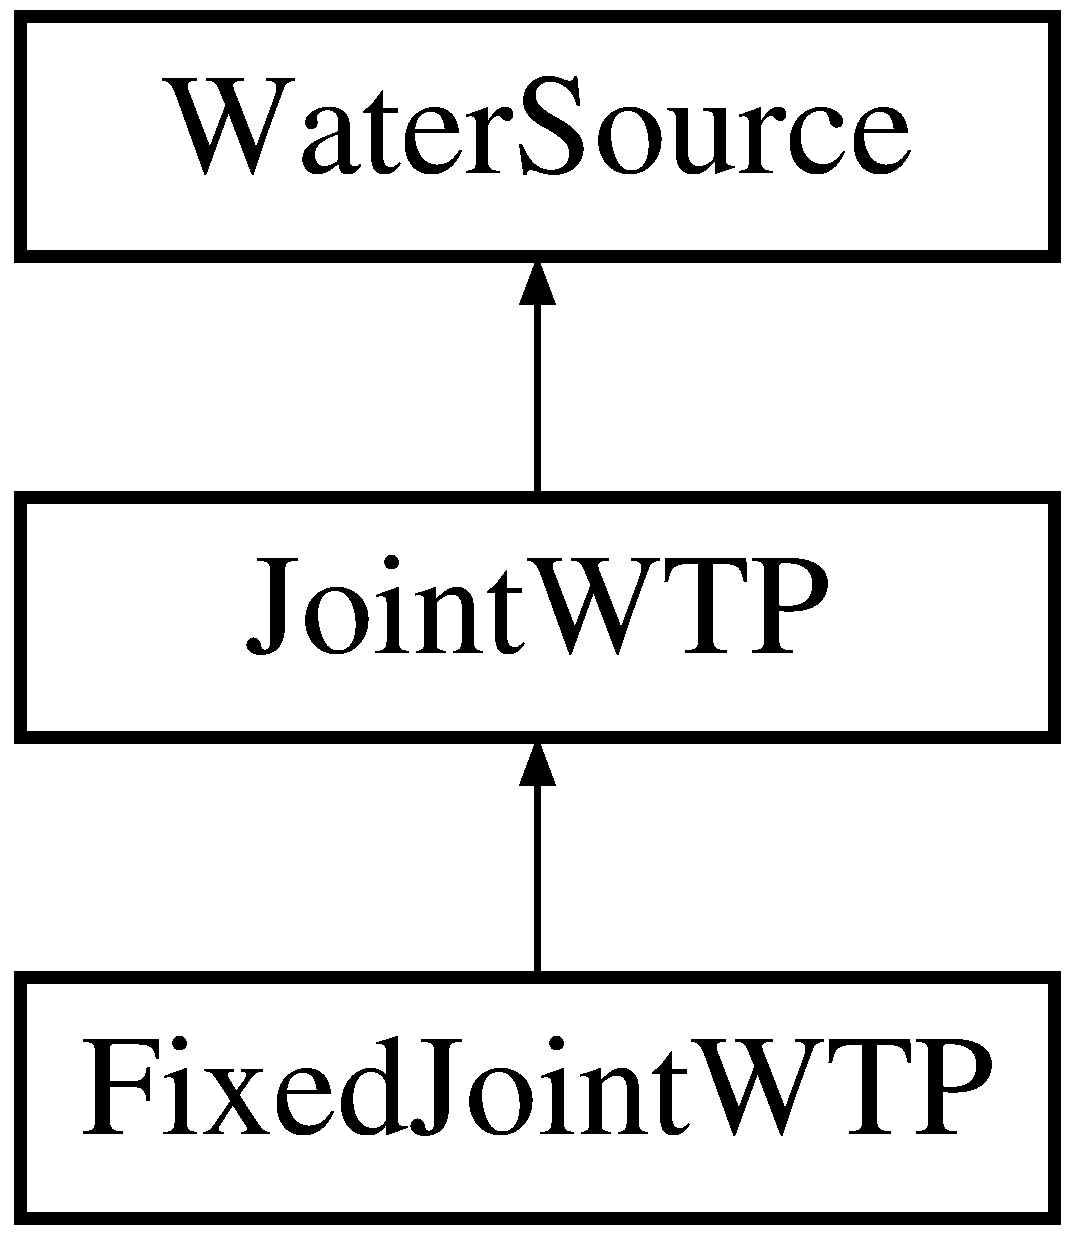
\includegraphics[height=3.000000cm]{classFixedJointWTP}
\end{center}
\end{figure}
\subsection*{Public Member Functions}
\begin{DoxyCompactItemize}
\item 
\mbox{\hyperlink{classFixedJointWTP_a4c9f0d469ea60620d3f2441d3c2f3aaf}{Fixed\+Joint\+W\+TP}} (const char $\ast$\mbox{\hyperlink{classWaterSource_a846ea74c5b453d014f594d41fee8c765}{name}}, const int \mbox{\hyperlink{classWaterSource_a6eafe5dfefd317877d1244e8a7c6e742}{id}}, const int \mbox{\hyperlink{classJointWTP_aa5830cb4d3013a004b7168f4dbf475eb}{parent\+\_\+reservoir\+\_\+\+ID}}, const int \mbox{\hyperlink{classJointWTP_a0e10a7f7ade04d5f3572f185de1b8653}{expansion\+\_\+sequence\+\_\+id}}, const double \mbox{\hyperlink{classWaterSource_a2fdfd5ff7d103e71108cf2a31babaccb}{total\+\_\+treatment\+\_\+capacity}}, vector$<$ int $>$ connected\+\_\+sources, vector$<$ int $>$ \&agreement\+\_\+utility\+\_\+ids, vector$<$ double $>$ \&fixed\+\_\+treatment\+\_\+capacity\+\_\+allocations, vector$<$ \mbox{\hyperlink{classBond}{Bond}} $\ast$$>$ \&\mbox{\hyperlink{classWaterSource_a413b094e11bdce62f4d82e5bb9e4706e}{bonds}}, const vector$<$ double $>$ \&construction\+\_\+time\+\_\+range, double permitting\+\_\+period)
\begin{DoxyCompactList}\small\item\em Constructs a \mbox{\hyperlink{classFixedJointWTP}{Fixed\+Joint\+W\+TP}} object. \end{DoxyCompactList}\item 
\mbox{\hyperlink{classFixedJointWTP_accf60b3a2b9907231a816135772261f8}{Fixed\+Joint\+W\+TP}} (const \mbox{\hyperlink{classFixedJointWTP}{Fixed\+Joint\+W\+TP}} \&fixed\+\_\+joint\+\_\+water\+\_\+treatment\+\_\+plant)
\begin{DoxyCompactList}\small\item\em Copy constructor for the \mbox{\hyperlink{classFixedJointWTP}{Fixed\+Joint\+W\+TP}} class. \end{DoxyCompactList}\item 
\mbox{\hyperlink{classFixedJointWTP_a9c42b1420843421c045feeb489b07b95}{$\sim$\+Fixed\+Joint\+W\+TP}} () override
\begin{DoxyCompactList}\small\item\em Destructor for the \mbox{\hyperlink{classFixedJointWTP}{Fixed\+Joint\+W\+TP}} class. \end{DoxyCompactList}\item 
\mbox{\hyperlink{classFixedJointWTP}{Fixed\+Joint\+W\+TP}} \& \mbox{\hyperlink{classFixedJointWTP_ad8cade8e61f861485b025cb0afe28c1a}{operator=}} (const \mbox{\hyperlink{classFixedJointWTP}{Fixed\+Joint\+W\+TP}} \&fixed\+\_\+joint\+\_\+water\+\_\+treatment\+\_\+plant)
\begin{DoxyCompactList}\small\item\em Assignment operator for the \mbox{\hyperlink{classFixedJointWTP}{Fixed\+Joint\+W\+TP}} class. \end{DoxyCompactList}\item 
void \mbox{\hyperlink{classFixedJointWTP_a68bfbed58c0106d896ef422ae9747d40}{apply\+Continuity}} (int week, double \mbox{\hyperlink{classWaterSource_a7a69b2e9b6030f1035e6cf44d2918ee5}{upstream\+\_\+source\+\_\+inflow}}, double wastewater\+\_\+discharge, vector$<$ double $>$ \&demand\+\_\+outflow) override
\begin{DoxyCompactList}\small\item\em Applies continuity for the \mbox{\hyperlink{classFixedJointWTP}{Fixed\+Joint\+W\+TP}} class. \end{DoxyCompactList}\item 
double \mbox{\hyperlink{classFixedJointWTP_a0874b64a650c002d7230bd95bc4817ef}{implement\+Initial\+Treatment\+Capacity}} (int utility\+\_\+id) override
\begin{DoxyCompactList}\small\item\em Implements the initial treatment capacity for a specific utility. \end{DoxyCompactList}\end{DoxyCompactItemize}
\subsection*{Additional Inherited Members}


\subsection{Detailed Description}
The {\ttfamily \mbox{\hyperlink{classFixedJointWTP}{Fixed\+Joint\+W\+TP}}} is a subclass of the {\ttfamily \mbox{\hyperlink{classJointWTP}{Joint\+W\+TP}}} class, which in turn is a subclass of the main {\ttfamily \mbox{\hyperlink{classWaterSource}{Water\+Source}}} class. This subclass represents the Joint W\+TP with fixed treatment capacity allocations to utilities. 

Created by dgorelic on 10/28/2019. 

\subsection{Constructor \& Destructor Documentation}
\mbox{\Hypertarget{classFixedJointWTP_a4c9f0d469ea60620d3f2441d3c2f3aaf}\label{classFixedJointWTP_a4c9f0d469ea60620d3f2441d3c2f3aaf}} 
\index{Fixed\+Joint\+W\+TP@{Fixed\+Joint\+W\+TP}!Fixed\+Joint\+W\+TP@{Fixed\+Joint\+W\+TP}}
\index{Fixed\+Joint\+W\+TP@{Fixed\+Joint\+W\+TP}!Fixed\+Joint\+W\+TP@{Fixed\+Joint\+W\+TP}}
\subsubsection{\texorpdfstring{Fixed\+Joint\+W\+T\+P()}{FixedJointWTP()}\hspace{0.1cm}{\footnotesize\ttfamily [1/2]}}
{\footnotesize\ttfamily Fixed\+Joint\+W\+T\+P\+::\+Fixed\+Joint\+W\+TP (\begin{DoxyParamCaption}\item[{const char $\ast$}]{name,  }\item[{const int}]{id,  }\item[{const int}]{parent\+\_\+reservoir\+\_\+\+ID,  }\item[{const int}]{expansion\+\_\+sequence\+\_\+id,  }\item[{const double}]{total\+\_\+treatment\+\_\+capacity,  }\item[{vector$<$ int $>$}]{connected\+\_\+sources,  }\item[{vector$<$ int $>$ \&}]{agreement\+\_\+utility\+\_\+ids,  }\item[{vector$<$ double $>$ \&}]{fixed\+\_\+treatment\+\_\+capacity\+\_\+allocations,  }\item[{vector$<$ \mbox{\hyperlink{classBond}{Bond}} $\ast$$>$ \&}]{bonds,  }\item[{const vector$<$ double $>$ \&}]{construction\+\_\+time\+\_\+range,  }\item[{double}]{permitting\+\_\+period }\end{DoxyParamCaption})}



Constructs a \mbox{\hyperlink{classFixedJointWTP}{Fixed\+Joint\+W\+TP}} object. 

This constructor initializes an instance of the {\ttfamily \mbox{\hyperlink{classFixedJointWTP}{Fixed\+Joint\+W\+TP}}} class, which represents a fixed allocation water treatment plant with a specified treatment capacity, parent reservoir, and various other parameters. It calls the base class {\ttfamily \mbox{\hyperlink{classJointWTP}{Joint\+W\+TP}}} constructor and sets the {\ttfamily permanent\+\_\+treatment\+\_\+allocations} pointer.


\begin{DoxyParams}{Parameters}
{\em name} & The name of the water treatment plant. \\
\hline
{\em id} & The unique identifier for the water treatment plant. \\
\hline
{\em parent\+\_\+reservoir\+\_\+\+ID} & The ID of the parent reservoir. \\
\hline
{\em expansion\+\_\+sequence\+\_\+id} & The ID representing the expansion sequence of the plant. \\
\hline
{\em total\+\_\+treatment\+\_\+capacity} & The total treatment capacity of the water treatment plant. \\
\hline
{\em connected\+\_\+sources} & A vector of integers representing the connected water sources to the treatment plant. \\
\hline
{\em agreement\+\_\+utility\+\_\+ids} & A vector of integers representing the utility I\+Ds associated with agreements for treatment capacity. \\
\hline
{\em fixed\+\_\+treatment\+\_\+capacity\+\_\+allocations} & A vector of doubles representing the fixed treatment capacity allocations for each utility. \\
\hline
{\em bonds} & A vector of pointers to {\ttfamily \mbox{\hyperlink{classBond}{Bond}}} objects representing the associated bonds with the treatment plant. \\
\hline
{\em construction\+\_\+time\+\_\+range} & A vector of doubles representing the construction time range for the treatment plant. \\
\hline
{\em permitting\+\_\+period} & The permitting period for the plant.\\
\hline
\end{DoxyParams}
\begin{DoxyReturn}{Returns}
A {\ttfamily \mbox{\hyperlink{classFixedJointWTP}{Fixed\+Joint\+W\+TP}}} object initialized with the specified parameters. 
\end{DoxyReturn}
\mbox{\Hypertarget{classFixedJointWTP_accf60b3a2b9907231a816135772261f8}\label{classFixedJointWTP_accf60b3a2b9907231a816135772261f8}} 
\index{Fixed\+Joint\+W\+TP@{Fixed\+Joint\+W\+TP}!Fixed\+Joint\+W\+TP@{Fixed\+Joint\+W\+TP}}
\index{Fixed\+Joint\+W\+TP@{Fixed\+Joint\+W\+TP}!Fixed\+Joint\+W\+TP@{Fixed\+Joint\+W\+TP}}
\subsubsection{\texorpdfstring{Fixed\+Joint\+W\+T\+P()}{FixedJointWTP()}\hspace{0.1cm}{\footnotesize\ttfamily [2/2]}}
{\footnotesize\ttfamily Fixed\+Joint\+W\+T\+P\+::\+Fixed\+Joint\+W\+TP (\begin{DoxyParamCaption}\item[{const \mbox{\hyperlink{classFixedJointWTP}{Fixed\+Joint\+W\+TP}} \&}]{fixed\+\_\+joint\+\_\+water\+\_\+treatment\+\_\+plant }\end{DoxyParamCaption})}



Copy constructor for the \mbox{\hyperlink{classFixedJointWTP}{Fixed\+Joint\+W\+TP}} class. 

This constructor creates a new {\ttfamily \mbox{\hyperlink{classFixedJointWTP}{Fixed\+Joint\+W\+TP}}} object as a copy of the provided {\ttfamily \mbox{\hyperlink{classFixedJointWTP}{Fixed\+Joint\+W\+TP}}} object. It copies all member variables from the given instance, including the {\ttfamily permanent\+\_\+treatment\+\_\+allocations} pointer.


\begin{DoxyParams}{Parameters}
{\em fixed\+\_\+joint\+\_\+water\+\_\+treatment\+\_\+plant} & The {\ttfamily \mbox{\hyperlink{classFixedJointWTP}{Fixed\+Joint\+W\+TP}}} object to copy.\\
\hline
\end{DoxyParams}
\begin{DoxyReturn}{Returns}
A new {\ttfamily \mbox{\hyperlink{classFixedJointWTP}{Fixed\+Joint\+W\+TP}}} object that is a copy of the provided object. 
\end{DoxyReturn}
\mbox{\Hypertarget{classFixedJointWTP_a9c42b1420843421c045feeb489b07b95}\label{classFixedJointWTP_a9c42b1420843421c045feeb489b07b95}} 
\index{Fixed\+Joint\+W\+TP@{Fixed\+Joint\+W\+TP}!````~Fixed\+Joint\+W\+TP@{$\sim$\+Fixed\+Joint\+W\+TP}}
\index{````~Fixed\+Joint\+W\+TP@{$\sim$\+Fixed\+Joint\+W\+TP}!Fixed\+Joint\+W\+TP@{Fixed\+Joint\+W\+TP}}
\subsubsection{\texorpdfstring{$\sim$\+Fixed\+Joint\+W\+T\+P()}{~FixedJointWTP()}}
{\footnotesize\ttfamily Fixed\+Joint\+W\+T\+P\+::$\sim$\+Fixed\+Joint\+W\+TP (\begin{DoxyParamCaption}{ }\end{DoxyParamCaption})\hspace{0.3cm}{\ttfamily [override]}}



Destructor for the \mbox{\hyperlink{classFixedJointWTP}{Fixed\+Joint\+W\+TP}} class. 

This destructor is the default destructor for the {\ttfamily \mbox{\hyperlink{classFixedJointWTP}{Fixed\+Joint\+W\+TP}}} class and ensures proper cleanup of resources when an object of this class is destroyed. Since the class does not manage any dynamic memory or resources directly, the destructor simply calls the default destructor of its base class ({\ttfamily \mbox{\hyperlink{classJointWTP}{Joint\+W\+TP}}}).

\begin{DoxyReturn}{Returns}
None 
\end{DoxyReturn}


\subsection{Member Function Documentation}
\mbox{\Hypertarget{classFixedJointWTP_a68bfbed58c0106d896ef422ae9747d40}\label{classFixedJointWTP_a68bfbed58c0106d896ef422ae9747d40}} 
\index{Fixed\+Joint\+W\+TP@{Fixed\+Joint\+W\+TP}!apply\+Continuity@{apply\+Continuity}}
\index{apply\+Continuity@{apply\+Continuity}!Fixed\+Joint\+W\+TP@{Fixed\+Joint\+W\+TP}}
\subsubsection{\texorpdfstring{apply\+Continuity()}{applyContinuity()}}
{\footnotesize\ttfamily void Fixed\+Joint\+W\+T\+P\+::apply\+Continuity (\begin{DoxyParamCaption}\item[{int}]{week,  }\item[{double}]{upstream\+\_\+source\+\_\+inflow,  }\item[{double}]{wastewater\+\_\+discharge,  }\item[{vector$<$ double $>$ \&}]{demand\+\_\+outflow }\end{DoxyParamCaption})\hspace{0.3cm}{\ttfamily [override]}, {\ttfamily [virtual]}}



Applies continuity for the \mbox{\hyperlink{classFixedJointWTP}{Fixed\+Joint\+W\+TP}} class. 

This function calls the base class ({\ttfamily \mbox{\hyperlink{classJointWTP}{Joint\+W\+TP}}}) implementation of {\ttfamily apply\+Continuity} to perform the necessary continuity checks and calculations for water treatment. It handles the inflows and outflows, ensuring the consistency of water volumes in the treatment process. This function overrides the virtual method in the base {\ttfamily \mbox{\hyperlink{classReservoir}{Reservoir}}} class.


\begin{DoxyParams}{Parameters}
{\em week} & The week for which continuity is being applied. \\
\hline
{\em upstream\+\_\+source\+\_\+inflow} & The volume of water inflow from upstream sources. \\
\hline
{\em wastewater\+\_\+discharge} & The volume of water from wastewater discharge. \\
\hline
{\em demand\+\_\+outflow} & A reference to a vector of water demand outflows for each utility.\\
\hline
\end{DoxyParams}
\begin{DoxyReturn}{Returns}
None. 
\end{DoxyReturn}


Implements \mbox{\hyperlink{classWaterSource_ac070445379fe706f65b977dade4f3fbc}{Water\+Source}}.

\mbox{\Hypertarget{classFixedJointWTP_a0874b64a650c002d7230bd95bc4817ef}\label{classFixedJointWTP_a0874b64a650c002d7230bd95bc4817ef}} 
\index{Fixed\+Joint\+W\+TP@{Fixed\+Joint\+W\+TP}!implement\+Initial\+Treatment\+Capacity@{implement\+Initial\+Treatment\+Capacity}}
\index{implement\+Initial\+Treatment\+Capacity@{implement\+Initial\+Treatment\+Capacity}!Fixed\+Joint\+W\+TP@{Fixed\+Joint\+W\+TP}}
\subsubsection{\texorpdfstring{implement\+Initial\+Treatment\+Capacity()}{implementInitialTreatmentCapacity()}}
{\footnotesize\ttfamily double Fixed\+Joint\+W\+T\+P\+::implement\+Initial\+Treatment\+Capacity (\begin{DoxyParamCaption}\item[{int}]{utility\+\_\+id }\end{DoxyParamCaption})\hspace{0.3cm}{\ttfamily [override]}, {\ttfamily [virtual]}}



Implements the initial treatment capacity for a specific utility. 

This function retrieves the initial treatment capacity allocated to a utility from the permanent treatment allocations. It assumes that the indices in the {\ttfamily permanent\+\_\+treatment\+\_\+allocations} vector correspond to the order of utility I\+Ds in the {\ttfamily agreement\+\_\+utility\+\_\+ids} vector. If the indices do not match, the returned value may be incorrect. This function overrides the virtual method in the base {\ttfamily \mbox{\hyperlink{classReservoir}{Reservoir}}} class.


\begin{DoxyParams}{Parameters}
{\em utility\+\_\+id} & The ID of the utility for which the initial treatment capacity is being retrieved.\\
\hline
\end{DoxyParams}
\begin{DoxyReturn}{Returns}
The initial treatment capacity allocated to the specified utility. 
\end{DoxyReturn}


Reimplemented from \mbox{\hyperlink{classJointWTP_ae8a2a5c4d5173b43d30fc9c1169574f8}{Joint\+W\+TP}}.

\mbox{\Hypertarget{classFixedJointWTP_ad8cade8e61f861485b025cb0afe28c1a}\label{classFixedJointWTP_ad8cade8e61f861485b025cb0afe28c1a}} 
\index{Fixed\+Joint\+W\+TP@{Fixed\+Joint\+W\+TP}!operator=@{operator=}}
\index{operator=@{operator=}!Fixed\+Joint\+W\+TP@{Fixed\+Joint\+W\+TP}}
\subsubsection{\texorpdfstring{operator=()}{operator=()}}
{\footnotesize\ttfamily \mbox{\hyperlink{classFixedJointWTP}{Fixed\+Joint\+W\+TP}}\& Fixed\+Joint\+W\+T\+P\+::operator= (\begin{DoxyParamCaption}\item[{const \mbox{\hyperlink{classFixedJointWTP}{Fixed\+Joint\+W\+TP}} \&}]{fixed\+\_\+joint\+\_\+water\+\_\+treatment\+\_\+plant }\end{DoxyParamCaption})}



Assignment operator for the \mbox{\hyperlink{classFixedJointWTP}{Fixed\+Joint\+W\+TP}} class. 

This operator allows for assignment of one {\ttfamily \mbox{\hyperlink{classFixedJointWTP}{Fixed\+Joint\+W\+TP}}} object to another. It ensures that the base class ({\ttfamily \mbox{\hyperlink{classJointWTP}{Joint\+W\+TP}}}) assignment operator is properly invoked and then returns the current object for chained assignments.


\begin{DoxyParams}{Parameters}
{\em fixed\+\_\+joint\+\_\+water\+\_\+treatment\+\_\+plant} & The {\ttfamily \mbox{\hyperlink{classFixedJointWTP}{Fixed\+Joint\+W\+TP}}} object to be assigned to the current object.\\
\hline
\end{DoxyParams}
\begin{DoxyReturn}{Returns}
A reference to the current {\ttfamily \mbox{\hyperlink{classFixedJointWTP}{Fixed\+Joint\+W\+TP}}} object after the assignment. 
\end{DoxyReturn}


The documentation for this class was generated from the following file\+:\begin{DoxyCompactItemize}
\item 
/home/fs02/pmr82\+\_\+0001/lbl59/\+Water\+Paths-\/doc/src/\+System\+Components/\+Water\+Sources/\mbox{\hyperlink{FixedJointWTP_8h}{Fixed\+Joint\+W\+T\+P.\+h}}\end{DoxyCompactItemize}

\hypertarget{classFloatingInterestBalloonPaymentBond}{}\section{Floating\+Interest\+Balloon\+Payment\+Bond Class Reference}
\label{classFloatingInterestBalloonPaymentBond}\index{Floating\+Interest\+Balloon\+Payment\+Bond@{Floating\+Interest\+Balloon\+Payment\+Bond}}


{\ttfamily \#include $<$Floating\+Interest\+Balloon\+Payment\+Bond.\+h$>$}

Inheritance diagram for Floating\+Interest\+Balloon\+Payment\+Bond\+:\begin{figure}[H]
\begin{center}
\leavevmode
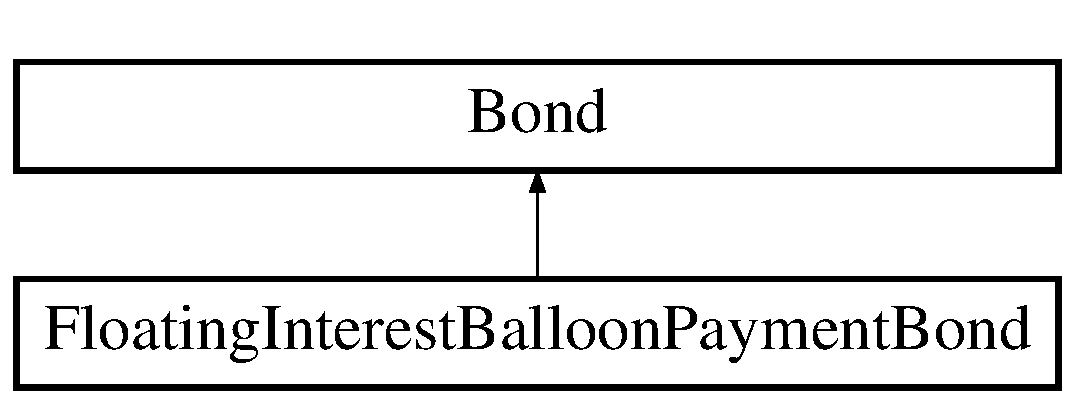
\includegraphics[height=2.000000cm]{classFloatingInterestBalloonPaymentBond}
\end{center}
\end{figure}
\subsection*{Public Member Functions}
\begin{DoxyCompactItemize}
\item 
\mbox{\hyperlink{classFloatingInterestBalloonPaymentBond_aa42f50447a3dd1bd6959e8c4bd0c2421_aa42f50447a3dd1bd6959e8c4bd0c2421}{Floating\+Interest\+Balloon\+Payment\+Bond}} (const int \mbox{\hyperlink{classBond_a7f75bcafbc16676ad6dbafbf40afae4a_a7f75bcafbc16676ad6dbafbf40afae4a}{id}}, const double \mbox{\hyperlink{classBond_ad98df7d28b398e620286f95ee085439b_ad98df7d28b398e620286f95ee085439b}{cost\+\_\+of\+\_\+capital}}, const double \mbox{\hyperlink{classBond_a4a227b6de2eeada118d82ab1633b1db8_a4a227b6de2eeada118d82ab1633b1db8}{n\+\_\+payments}}, const vector$<$ double $>$ \mbox{\hyperlink{classFloatingInterestBalloonPaymentBond_a36c73466753c976e513c6763f79f58ad_a36c73466753c976e513c6763f79f58ad}{interest\+\_\+rate\+\_\+series}}, vector$<$ int $>$ \mbox{\hyperlink{classBond_ae8dd46fcbf95c993460ffe4ea1f52739_ae8dd46fcbf95c993460ffe4ea1f52739}{pay\+\_\+on\+\_\+weeks}})
\item 
\mbox{\hyperlink{classFloatingInterestBalloonPaymentBond_a9732cbf82ecc484237071bb681f7dc63_a9732cbf82ecc484237071bb681f7dc63}{Floating\+Interest\+Balloon\+Payment\+Bond}} (const int \mbox{\hyperlink{classBond_a7f75bcafbc16676ad6dbafbf40afae4a_a7f75bcafbc16676ad6dbafbf40afae4a}{id}}, const double \mbox{\hyperlink{classBond_ad98df7d28b398e620286f95ee085439b_ad98df7d28b398e620286f95ee085439b}{cost\+\_\+of\+\_\+capital}}, double \mbox{\hyperlink{classBond_a4a227b6de2eeada118d82ab1633b1db8_a4a227b6de2eeada118d82ab1633b1db8}{n\+\_\+payments}}, const vector$<$ double $>$ \mbox{\hyperlink{classFloatingInterestBalloonPaymentBond_a36c73466753c976e513c6763f79f58ad_a36c73466753c976e513c6763f79f58ad}{interest\+\_\+rate\+\_\+series}}, vector$<$ int $>$ \mbox{\hyperlink{classBond_ae8dd46fcbf95c993460ffe4ea1f52739_ae8dd46fcbf95c993460ffe4ea1f52739}{pay\+\_\+on\+\_\+weeks}}, const int starts\+\_\+paying\+\_\+after\+\_\+n\+\_\+years)
\item 
double \mbox{\hyperlink{classFloatingInterestBalloonPaymentBond_a0009a0b12e0ebeb15952561513ddc901_a0009a0b12e0ebeb15952561513ddc901}{get\+Debt\+Service}} (int week) override
\item 
double \mbox{\hyperlink{classFloatingInterestBalloonPaymentBond_a90205e26e09eef1227f8c0671ca4fce2_a90205e26e09eef1227f8c0671ca4fce2}{get\+Net\+Present\+Value\+At\+Issuance}} (double yearly\+\_\+discount\+\_\+rate, int week) const override
\item 
void \mbox{\hyperlink{classFloatingInterestBalloonPaymentBond_a4cf110f320c92f5eca9aed952e0b527a_a4cf110f320c92f5eca9aed952e0b527a}{issue\+Bond}} (int week, int construction\+\_\+time, double bond\+\_\+term\+\_\+multiplier, double bond\+\_\+interest\+\_\+rate\+\_\+multiplier) override
\end{DoxyCompactItemize}
\subsection*{Private Attributes}
\begin{DoxyCompactItemize}
\item 
vector$<$ double $>$ \mbox{\hyperlink{classFloatingInterestBalloonPaymentBond_a36c73466753c976e513c6763f79f58ad_a36c73466753c976e513c6763f79f58ad}{interest\+\_\+rate\+\_\+series}}
\item 
const int \mbox{\hyperlink{classFloatingInterestBalloonPaymentBond_a439428fff4f2d4ba5d0b593e5d30687f_a439428fff4f2d4ba5d0b593e5d30687f}{begin\+\_\+repayment\+\_\+after\+\_\+n\+\_\+years}}
\item 
int \mbox{\hyperlink{classFloatingInterestBalloonPaymentBond_afc1a77eb5d799201c7ef5c52ef5df374_afc1a77eb5d799201c7ef5c52ef5df374}{n\+\_\+payments\+\_\+made}} = 0
\end{DoxyCompactItemize}
\subsection*{Additional Inherited Members}


\subsection{Constructor \& Destructor Documentation}
\mbox{\Hypertarget{classFloatingInterestBalloonPaymentBond_aa42f50447a3dd1bd6959e8c4bd0c2421_aa42f50447a3dd1bd6959e8c4bd0c2421}\label{classFloatingInterestBalloonPaymentBond_aa42f50447a3dd1bd6959e8c4bd0c2421_aa42f50447a3dd1bd6959e8c4bd0c2421}} 
\index{Floating\+Interest\+Balloon\+Payment\+Bond@{Floating\+Interest\+Balloon\+Payment\+Bond}!Floating\+Interest\+Balloon\+Payment\+Bond@{Floating\+Interest\+Balloon\+Payment\+Bond}}
\index{Floating\+Interest\+Balloon\+Payment\+Bond@{Floating\+Interest\+Balloon\+Payment\+Bond}!Floating\+Interest\+Balloon\+Payment\+Bond@{Floating\+Interest\+Balloon\+Payment\+Bond}}
\subsubsection{\texorpdfstring{Floating\+Interest\+Balloon\+Payment\+Bond()}{FloatingInterestBalloonPaymentBond()}\hspace{0.1cm}{\footnotesize\ttfamily [1/2]}}
{\footnotesize\ttfamily Floating\+Interest\+Balloon\+Payment\+Bond\+::\+Floating\+Interest\+Balloon\+Payment\+Bond (\begin{DoxyParamCaption}\item[{const int}]{id,  }\item[{const double}]{cost\+\_\+of\+\_\+capital,  }\item[{const double}]{n\+\_\+payments,  }\item[{const vector$<$ double $>$}]{interest\+\_\+rate\+\_\+series,  }\item[{vector$<$ int $>$}]{pay\+\_\+on\+\_\+weeks }\end{DoxyParamCaption})}


\begin{DoxyParams}{Parameters}
{\em id} & \\
\hline
{\em cost\+\_\+of\+\_\+capital} & \\
\hline
{\em n\+\_\+payments} & \\
\hline
{\em interest\+\_\+rate\+\_\+series} & Interest time series beginning from week 0 of simulation. \\
\hline
{\em pay\+\_\+on\+\_\+weeks} & \\
\hline
\end{DoxyParams}
\mbox{\Hypertarget{classFloatingInterestBalloonPaymentBond_a9732cbf82ecc484237071bb681f7dc63_a9732cbf82ecc484237071bb681f7dc63}\label{classFloatingInterestBalloonPaymentBond_a9732cbf82ecc484237071bb681f7dc63_a9732cbf82ecc484237071bb681f7dc63}} 
\index{Floating\+Interest\+Balloon\+Payment\+Bond@{Floating\+Interest\+Balloon\+Payment\+Bond}!Floating\+Interest\+Balloon\+Payment\+Bond@{Floating\+Interest\+Balloon\+Payment\+Bond}}
\index{Floating\+Interest\+Balloon\+Payment\+Bond@{Floating\+Interest\+Balloon\+Payment\+Bond}!Floating\+Interest\+Balloon\+Payment\+Bond@{Floating\+Interest\+Balloon\+Payment\+Bond}}
\subsubsection{\texorpdfstring{Floating\+Interest\+Balloon\+Payment\+Bond()}{FloatingInterestBalloonPaymentBond()}\hspace{0.1cm}{\footnotesize\ttfamily [2/2]}}
{\footnotesize\ttfamily Floating\+Interest\+Balloon\+Payment\+Bond\+::\+Floating\+Interest\+Balloon\+Payment\+Bond (\begin{DoxyParamCaption}\item[{const int}]{id,  }\item[{const double}]{cost\+\_\+of\+\_\+capital,  }\item[{double}]{n\+\_\+payments,  }\item[{const vector$<$ double $>$}]{interest\+\_\+rate\+\_\+series,  }\item[{vector$<$ int $>$}]{pay\+\_\+on\+\_\+weeks,  }\item[{const int}]{starts\+\_\+paying\+\_\+after\+\_\+n\+\_\+years }\end{DoxyParamCaption})}


\begin{DoxyParams}{Parameters}
{\em id} & \\
\hline
{\em cost\+\_\+of\+\_\+capital} & \\
\hline
{\em n\+\_\+payments} & \\
\hline
{\em interest\+\_\+rate\+\_\+series} & Interest time series beginning from week 0 of simulation. \\
\hline
{\em pay\+\_\+on\+\_\+weeks} & \\
\hline
{\em starts\+\_\+paying\+\_\+after\+\_\+n\+\_\+years} & \\
\hline
\end{DoxyParams}


\subsection{Member Function Documentation}
\mbox{\Hypertarget{classFloatingInterestBalloonPaymentBond_a0009a0b12e0ebeb15952561513ddc901_a0009a0b12e0ebeb15952561513ddc901}\label{classFloatingInterestBalloonPaymentBond_a0009a0b12e0ebeb15952561513ddc901_a0009a0b12e0ebeb15952561513ddc901}} 
\index{Floating\+Interest\+Balloon\+Payment\+Bond@{Floating\+Interest\+Balloon\+Payment\+Bond}!get\+Debt\+Service@{get\+Debt\+Service}}
\index{get\+Debt\+Service@{get\+Debt\+Service}!Floating\+Interest\+Balloon\+Payment\+Bond@{Floating\+Interest\+Balloon\+Payment\+Bond}}
\subsubsection{\texorpdfstring{get\+Debt\+Service()}{getDebtService()}}
{\footnotesize\ttfamily double Floating\+Interest\+Balloon\+Payment\+Bond\+::get\+Debt\+Service (\begin{DoxyParamCaption}\item[{int}]{week }\end{DoxyParamCaption})\hspace{0.3cm}{\ttfamily [override]}, {\ttfamily [virtual]}}

Calculates debt service payment for a give week. 
\begin{DoxyParams}{Parameters}
{\em week} & \\
\hline
\end{DoxyParams}
\begin{DoxyReturn}{Returns}

\end{DoxyReturn}
If there are still payments to be made, repayment has begun, and this is a payment week, issue payment. 

Implements \mbox{\hyperlink{classBond_a98d8ecaf4b36319674ebd220598996bc_a98d8ecaf4b36319674ebd220598996bc}{Bond}}.

\mbox{\Hypertarget{classFloatingInterestBalloonPaymentBond_a90205e26e09eef1227f8c0671ca4fce2_a90205e26e09eef1227f8c0671ca4fce2}\label{classFloatingInterestBalloonPaymentBond_a90205e26e09eef1227f8c0671ca4fce2_a90205e26e09eef1227f8c0671ca4fce2}} 
\index{Floating\+Interest\+Balloon\+Payment\+Bond@{Floating\+Interest\+Balloon\+Payment\+Bond}!get\+Net\+Present\+Value\+At\+Issuance@{get\+Net\+Present\+Value\+At\+Issuance}}
\index{get\+Net\+Present\+Value\+At\+Issuance@{get\+Net\+Present\+Value\+At\+Issuance}!Floating\+Interest\+Balloon\+Payment\+Bond@{Floating\+Interest\+Balloon\+Payment\+Bond}}
\subsubsection{\texorpdfstring{get\+Net\+Present\+Value\+At\+Issuance()}{getNetPresentValueAtIssuance()}}
{\footnotesize\ttfamily double Floating\+Interest\+Balloon\+Payment\+Bond\+::get\+Net\+Present\+Value\+At\+Issuance (\begin{DoxyParamCaption}\item[{double}]{yearly\+\_\+discount\+\_\+rate,  }\item[{int}]{week }\end{DoxyParamCaption}) const\hspace{0.3cm}{\ttfamily [override]}, {\ttfamily [virtual]}}



Implements \mbox{\hyperlink{classBond_a5997278813deb16aa5d01bbca8ecc7b2_a5997278813deb16aa5d01bbca8ecc7b2}{Bond}}.

\mbox{\Hypertarget{classFloatingInterestBalloonPaymentBond_a4cf110f320c92f5eca9aed952e0b527a_a4cf110f320c92f5eca9aed952e0b527a}\label{classFloatingInterestBalloonPaymentBond_a4cf110f320c92f5eca9aed952e0b527a_a4cf110f320c92f5eca9aed952e0b527a}} 
\index{Floating\+Interest\+Balloon\+Payment\+Bond@{Floating\+Interest\+Balloon\+Payment\+Bond}!issue\+Bond@{issue\+Bond}}
\index{issue\+Bond@{issue\+Bond}!Floating\+Interest\+Balloon\+Payment\+Bond@{Floating\+Interest\+Balloon\+Payment\+Bond}}
\subsubsection{\texorpdfstring{issue\+Bond()}{issueBond()}}
{\footnotesize\ttfamily void Floating\+Interest\+Balloon\+Payment\+Bond\+::issue\+Bond (\begin{DoxyParamCaption}\item[{int}]{week,  }\item[{int}]{construction\+\_\+time,  }\item[{double}]{bond\+\_\+term\+\_\+multiplier,  }\item[{double}]{bond\+\_\+interest\+\_\+rate\+\_\+multiplier }\end{DoxyParamCaption})\hspace{0.3cm}{\ttfamily [override]}, {\ttfamily [virtual]}}

Multiply entire interest time time series by R\+DM factor. 

Reimplemented from \mbox{\hyperlink{classBond_a377db8c18b83c4666e46686bc26adef1_a377db8c18b83c4666e46686bc26adef1}{Bond}}.



\subsection{Field Documentation}
\mbox{\Hypertarget{classFloatingInterestBalloonPaymentBond_a439428fff4f2d4ba5d0b593e5d30687f_a439428fff4f2d4ba5d0b593e5d30687f}\label{classFloatingInterestBalloonPaymentBond_a439428fff4f2d4ba5d0b593e5d30687f_a439428fff4f2d4ba5d0b593e5d30687f}} 
\index{Floating\+Interest\+Balloon\+Payment\+Bond@{Floating\+Interest\+Balloon\+Payment\+Bond}!begin\+\_\+repayment\+\_\+after\+\_\+n\+\_\+years@{begin\+\_\+repayment\+\_\+after\+\_\+n\+\_\+years}}
\index{begin\+\_\+repayment\+\_\+after\+\_\+n\+\_\+years@{begin\+\_\+repayment\+\_\+after\+\_\+n\+\_\+years}!Floating\+Interest\+Balloon\+Payment\+Bond@{Floating\+Interest\+Balloon\+Payment\+Bond}}
\subsubsection{\texorpdfstring{begin\+\_\+repayment\+\_\+after\+\_\+n\+\_\+years}{begin\_repayment\_after\_n\_years}}
{\footnotesize\ttfamily const int Floating\+Interest\+Balloon\+Payment\+Bond\+::begin\+\_\+repayment\+\_\+after\+\_\+n\+\_\+years\hspace{0.3cm}{\ttfamily [private]}}

\mbox{\Hypertarget{classFloatingInterestBalloonPaymentBond_a36c73466753c976e513c6763f79f58ad_a36c73466753c976e513c6763f79f58ad}\label{classFloatingInterestBalloonPaymentBond_a36c73466753c976e513c6763f79f58ad_a36c73466753c976e513c6763f79f58ad}} 
\index{Floating\+Interest\+Balloon\+Payment\+Bond@{Floating\+Interest\+Balloon\+Payment\+Bond}!interest\+\_\+rate\+\_\+series@{interest\+\_\+rate\+\_\+series}}
\index{interest\+\_\+rate\+\_\+series@{interest\+\_\+rate\+\_\+series}!Floating\+Interest\+Balloon\+Payment\+Bond@{Floating\+Interest\+Balloon\+Payment\+Bond}}
\subsubsection{\texorpdfstring{interest\+\_\+rate\+\_\+series}{interest\_rate\_series}}
{\footnotesize\ttfamily vector$<$double$>$ Floating\+Interest\+Balloon\+Payment\+Bond\+::interest\+\_\+rate\+\_\+series\hspace{0.3cm}{\ttfamily [private]}}

\mbox{\Hypertarget{classFloatingInterestBalloonPaymentBond_afc1a77eb5d799201c7ef5c52ef5df374_afc1a77eb5d799201c7ef5c52ef5df374}\label{classFloatingInterestBalloonPaymentBond_afc1a77eb5d799201c7ef5c52ef5df374_afc1a77eb5d799201c7ef5c52ef5df374}} 
\index{Floating\+Interest\+Balloon\+Payment\+Bond@{Floating\+Interest\+Balloon\+Payment\+Bond}!n\+\_\+payments\+\_\+made@{n\+\_\+payments\+\_\+made}}
\index{n\+\_\+payments\+\_\+made@{n\+\_\+payments\+\_\+made}!Floating\+Interest\+Balloon\+Payment\+Bond@{Floating\+Interest\+Balloon\+Payment\+Bond}}
\subsubsection{\texorpdfstring{n\+\_\+payments\+\_\+made}{n\_payments\_made}}
{\footnotesize\ttfamily int Floating\+Interest\+Balloon\+Payment\+Bond\+::n\+\_\+payments\+\_\+made = 0\hspace{0.3cm}{\ttfamily [private]}}



The documentation for this class was generated from the following files\+:\begin{DoxyCompactItemize}
\item 
src/\+System\+Components/\+Bonds/\mbox{\hyperlink{FloatingInterestBalloonPaymentBond_8h}{Floating\+Interest\+Balloon\+Payment\+Bond.\+h}}\item 
src/\+System\+Components/\+Bonds/\mbox{\hyperlink{FloatingInterestBalloonPaymentBond_8cpp}{Floating\+Interest\+Balloon\+Payment\+Bond.\+cpp}}\end{DoxyCompactItemize}

\hypertarget{structinfraRank}{}\section{infra\+Rank Struct Reference}
\label{structinfraRank}\index{infra\+Rank@{infra\+Rank}}


{\ttfamily \#include $<$Problem.\+h$>$}

\subsection*{Public Member Functions}
\begin{DoxyCompactItemize}
\item 
\mbox{\hyperlink{structinfraRank_aa50dcfdcee689bd1484c9ac2b09bc694_aa50dcfdcee689bd1484c9ac2b09bc694}{infra\+Rank}} (int \mbox{\hyperlink{structinfraRank_ace3640f7fdc691b68111cf07e0eabaae_ace3640f7fdc691b68111cf07e0eabaae}{id}}, double \mbox{\hyperlink{structinfraRank_a1bb966369809456d65bd4e2d4e19d775_a1bb966369809456d65bd4e2d4e19d775}{xreal}})
\end{DoxyCompactItemize}
\subsection*{Data Fields}
\begin{DoxyCompactItemize}
\item 
int \mbox{\hyperlink{structinfraRank_ace3640f7fdc691b68111cf07e0eabaae_ace3640f7fdc691b68111cf07e0eabaae}{id}}
\item 
double \mbox{\hyperlink{structinfraRank_a1bb966369809456d65bd4e2d4e19d775_a1bb966369809456d65bd4e2d4e19d775}{xreal}}
\end{DoxyCompactItemize}


\subsection{Constructor \& Destructor Documentation}
\mbox{\Hypertarget{structinfraRank_aa50dcfdcee689bd1484c9ac2b09bc694_aa50dcfdcee689bd1484c9ac2b09bc694}\label{structinfraRank_aa50dcfdcee689bd1484c9ac2b09bc694_aa50dcfdcee689bd1484c9ac2b09bc694}} 
\index{infra\+Rank@{infra\+Rank}!infra\+Rank@{infra\+Rank}}
\index{infra\+Rank@{infra\+Rank}!infra\+Rank@{infra\+Rank}}
\subsubsection{\texorpdfstring{infra\+Rank()}{infraRank()}}
{\footnotesize\ttfamily infra\+Rank\+::infra\+Rank (\begin{DoxyParamCaption}\item[{int}]{id,  }\item[{double}]{xreal }\end{DoxyParamCaption})\hspace{0.3cm}{\ttfamily [inline]}}



\subsection{Field Documentation}
\mbox{\Hypertarget{structinfraRank_ace3640f7fdc691b68111cf07e0eabaae_ace3640f7fdc691b68111cf07e0eabaae}\label{structinfraRank_ace3640f7fdc691b68111cf07e0eabaae_ace3640f7fdc691b68111cf07e0eabaae}} 
\index{infra\+Rank@{infra\+Rank}!id@{id}}
\index{id@{id}!infra\+Rank@{infra\+Rank}}
\subsubsection{\texorpdfstring{id}{id}}
{\footnotesize\ttfamily int infra\+Rank\+::id}

\mbox{\Hypertarget{structinfraRank_a1bb966369809456d65bd4e2d4e19d775_a1bb966369809456d65bd4e2d4e19d775}\label{structinfraRank_a1bb966369809456d65bd4e2d4e19d775_a1bb966369809456d65bd4e2d4e19d775}} 
\index{infra\+Rank@{infra\+Rank}!xreal@{xreal}}
\index{xreal@{xreal}!infra\+Rank@{infra\+Rank}}
\subsubsection{\texorpdfstring{xreal}{xreal}}
{\footnotesize\ttfamily double infra\+Rank\+::xreal}



The documentation for this struct was generated from the following file\+:\begin{DoxyCompactItemize}
\item 
src/\+Problem/\+Base/\mbox{\hyperlink{Problem_8h}{Problem.\+h}}\end{DoxyCompactItemize}

\hypertarget{classInfrastructureManager}{}\section{Infrastructure\+Manager Class Reference}
\label{classInfrastructureManager}\index{Infrastructure\+Manager@{Infrastructure\+Manager}}


{\ttfamily \#include $<$Infrastructure\+Manager.\+h$>$}

\subsection*{Public Member Functions}
\begin{DoxyCompactItemize}
\item 
\mbox{\hyperlink{classInfrastructureManager_a2720f467b660e0f63f265e7957ca0139}{Infrastructure\+Manager}} (int id, const vector$<$ double $>$ \&infra\+\_\+construction\+\_\+triggers, const vector$<$ vector$<$ int $>$$>$ \&infra\+\_\+if\+\_\+built\+\_\+remove, double infra\+\_\+discount\+\_\+rate, double bond\+\_\+term, double bond\+\_\+interest\+\_\+rate, vector$<$ int $>$ rof\+\_\+infra\+\_\+construction\+\_\+order, vector$<$ int $>$ demand\+\_\+infra\+\_\+construction\+\_\+order)
\begin{DoxyCompactList}\small\item\em Constructs an \mbox{\hyperlink{classInfrastructureManager}{Infrastructure\+Manager}} object. \end{DoxyCompactList}\item 
\mbox{\hyperlink{classInfrastructureManager_a435ec4cb56238c6e1d93e37783f3a03a}{Infrastructure\+Manager}} ()
\begin{DoxyCompactList}\small\item\em Basic constructor a new Infrastructure Manager object. \end{DoxyCompactList}\item 
\mbox{\hyperlink{classInfrastructureManager}{Infrastructure\+Manager}} \& \mbox{\hyperlink{classInfrastructureManager_ad016a00ca49b1896e94a04f723209a64}{operator=}} (const \mbox{\hyperlink{classInfrastructureManager}{Infrastructure\+Manager}} \&infrastructure\+\_\+manager)
\begin{DoxyCompactList}\small\item\em An assignment operator that copies the values of the infrastructure manager object to another infrastructure manager object. \end{DoxyCompactList}\item 
\mbox{\hyperlink{classInfrastructureManager_a9d1fe6a0325a3705dbfabb92afbe9055}{Infrastructure\+Manager}} (\mbox{\hyperlink{classInfrastructureManager}{Infrastructure\+Manager}} \&infrastructure\+\_\+manager)
\begin{DoxyCompactList}\small\item\em Constructs a new Infrastructure Manager object from an existing Infrastructure Manager object. \end{DoxyCompactList}\item 
vector$<$ double $>$ \mbox{\hyperlink{classInfrastructureManager_a23888a04e8cb5e2fb7a36b2258d4a259}{rearrange\+Infra\+Rof\+Vector}} (const vector$<$ double $>$ \&infra\+\_\+construction\+\_\+triggers, const vector$<$ int $>$ \&rof\+\_\+infra\+\_\+construction\+\_\+order, const vector$<$ int $>$ \&demand\+\_\+infra\+\_\+construction\+\_\+order)
\begin{DoxyCompactList}\small\item\em Rearranges the infrastructure construction trigger vector to match the specified order of construction based on R\+OF and demand. \end{DoxyCompactList}\item 
void \mbox{\hyperlink{classInfrastructureManager_a9972a27ff6d08b7c1226d703ac700a94}{set\+Water\+Source\+Online}} (unsigned int source\+\_\+id, int week, double \&total\+\_\+storage\+\_\+capacity, double \&total\+\_\+treatment\+\_\+capacity, double \&total\+\_\+available\+\_\+volume, double \&total\+\_\+stored\+\_\+volume)
\begin{DoxyCompactList}\small\item\em Identifies the type of water source and sets a water source online and updates related capacities and volumes. \end{DoxyCompactList}\item 
void \mbox{\hyperlink{classInfrastructureManager_ad40c7049e76f7d097f1dd066c84d5c79}{water\+Treatment\+Plant\+Construction\+Handler}} (unsigned int source\+\_\+id, double \&total\+\_\+storage\+\_\+capacity)
\begin{DoxyCompactList}\small\item\em Handles the construction of a water treatment plant and updates the associated water source\textquotesingle{}s capacity and priority lists. \end{DoxyCompactList}\item 
void \mbox{\hyperlink{classInfrastructureManager_ad4dc157110b29560cd47501ba67bcba3}{reservoir\+Expansion\+Construction\+Handler}} (unsigned int source\+\_\+id)
\begin{DoxyCompactList}\small\item\em Handles the construction of a reservoir expansion by adding capacity to its parent reservoir. \end{DoxyCompactList}\item 
void \mbox{\hyperlink{classInfrastructureManager_a1eb260820a0127294d18d160cb146db9}{source\+Relocation\+Construction\+Handler}} (unsigned int source\+\_\+id)
\begin{DoxyCompactList}\small\item\em Handles the relocation of a water source by updating its allocation fractions and activating it. \end{DoxyCompactList}\item 
void \mbox{\hyperlink{classInfrastructureManager_abf6d8d9891abddfe08df0bb7677eee35}{remove\+Related\+Sources\+From\+Queue}} (int next\+\_\+construction)
\begin{DoxyCompactList}\small\item\em Checks if piece of infrastructure to be built next prevents another one from being build. If yes, remove the latter from the queue. \end{DoxyCompactList}\item 
int \mbox{\hyperlink{classInfrastructureManager_a06c7a2df105a2a8dd3ef625ad42694ce}{infrastructure\+Construction\+Handler}} (double long\+\_\+term\+\_\+rof, int week, double past\+\_\+year\+\_\+average\+\_\+demand, double \&total\+\_\+storage\+\_\+capacity, double \&total\+\_\+treatment\+\_\+capacity, double \&total\+\_\+available\+\_\+volume, double \&total\+\_\+stored\+\_\+volume)
\begin{DoxyCompactList}\small\item\em Handles the initiation, progression, and completion of infrastructure construction based on demand and reliability triggers. Also handles the accounting and financing of the infrastructure. \end{DoxyCompactList}\item 
void \mbox{\hyperlink{classInfrastructureManager_aaa79bdb84fc23597c4a8b3776dc26f5d}{force\+Infrastructure\+Construction}} (int week, vector$<$ int $>$ new\+\_\+infra\+\_\+triggered)
\begin{DoxyCompactList}\small\item\em Forces the construction of specified infrastructure options for all other utilities if they are in the queue. \end{DoxyCompactList}\item 
void \mbox{\hyperlink{classInfrastructureManager_a7d60e4abff73890519ced487c74f2675}{begin\+Construction}} (int week, int infra\+\_\+id)
\begin{DoxyCompactList}\small\item\em Initiates the construction of the specified infrastructure and records the start and end dates. \end{DoxyCompactList}\item 
void \mbox{\hyperlink{classInfrastructureManager_ab66bdc91a6f60c6aea6ce0bf179df913}{add\+Water\+Source\+To\+Online\+Lists}} (int source\+\_\+id, double \&total\+\_\+storage\+\_\+capacity, double \&total\+\_\+treatment\+\_\+capacity, double \&total\+\_\+available\+\_\+volume, double \&total\+\_\+stored\+\_\+volume)
\begin{DoxyCompactList}\small\item\em Adds a water source to the utility\textquotesingle{}s online lists and updates the relevant capacity and volume totals. \end{DoxyCompactList}\item 
void \mbox{\hyperlink{classInfrastructureManager_a3950df03bc8fd5743aefeca4c3d7bf98}{add\+Water\+Source}} (\mbox{\hyperlink{classWaterSource}{Water\+Source}} $\ast$water\+\_\+source)
\begin{DoxyCompactList}\small\item\em Adds a water source to the construction management system. \end{DoxyCompactList}\item 
void \mbox{\hyperlink{classInfrastructureManager_a8ff698443fd4f32e28677aa9ef34c2dc}{connect\+Water\+Sources\+Vectors\+To\+Utilitys}} (vector$<$ \mbox{\hyperlink{classWaterSource}{Water\+Source}} $\ast$$>$ \&water\+\_\+sources, vector$<$ int $>$ \&priority\+\_\+draw\+\_\+water\+\_\+source, vector$<$ int $>$ \&non\+\_\+priority\+\_\+draw\+\_\+water\+\_\+source)
\begin{DoxyCompactList}\small\item\em Connects the provided water source vectors to the utility. \end{DoxyCompactList}\item 
const vector$<$ bool $>$ \& \mbox{\hyperlink{classInfrastructureManager_ad598850bb18f5a6fc81a0e2bc7885ef2}{get\+Under\+\_\+construction}} () const
\begin{DoxyCompactList}\small\item\em Retrieves the list of infrastructure construction statuses. \end{DoxyCompactList}\item 
void \mbox{\hyperlink{classInfrastructureManager_aed62e86a9737e385c821d44ea70922e9}{intake\+Expansion\+Construction\+Handler}} (unsigned int source\+\_\+id)
\begin{DoxyCompactList}\small\item\em Handles the construction of an intake expansion. \end{DoxyCompactList}\item 
void \mbox{\hyperlink{classInfrastructureManager_a669881b881b090b3dd8fe70e3ffbf7f6}{water\+Treatment\+Plant\+Joint\+Construction\+Handler}} (unsigned int source\+\_\+id, double \&total\+\_\+storage\+\_\+capacity)
\begin{DoxyCompactList}\small\item\em Handles the construction of a joint water treatment plant (W\+TP) with either fixed or variable treatment allocations. \end{DoxyCompactList}\item 
void \mbox{\hyperlink{classInfrastructureManager_a4fc2e6e4fa74374b6669f5360dcda9d9}{allocated\+Intake\+Expansion\+Construction\+Handler}} (unsigned int source\+\_\+id)
\begin{DoxyCompactList}\small\item\em Handles the construction of an allocated intake expansion and updates related capacities. \end{DoxyCompactList}\item 
void \mbox{\hyperlink{classInfrastructureManager_a4eca31074654eb197ba33342eee3bd32}{check\+For\+Sequence\+Projects}} (int original\+\_\+build\+\_\+id)
\begin{DoxyCompactList}\small\item\em Checks if a water source is part of a sequence of projects and adjusts capital costs based on the sequence. \end{DoxyCompactList}\item 
const vector$<$ int $>$ \& \mbox{\hyperlink{classInfrastructureManager_a0f944c7704cc5418ba58b71c7a1e15a7}{get\+Rof\+\_\+infra\+\_\+construction\+\_\+order}} () const
\begin{DoxyCompactList}\small\item\em Retrieves the list of water sources in the R\+OF infrastructure construction order. \end{DoxyCompactList}\item 
const vector$<$ int $>$ \& \mbox{\hyperlink{classInfrastructureManager_aac2a99dbffe7f784f09de907ad384d8b}{get\+Demand\+\_\+infra\+\_\+construction\+\_\+order}} () const
\begin{DoxyCompactList}\small\item\em Retrieves the list of water sources in the demand infrastructure construction order. \end{DoxyCompactList}\item 
const vector$<$ int $>$ \& \mbox{\hyperlink{classInfrastructureManager_a540f233692981645d52af7f1de087dbf}{get\+Infra\+\_\+built\+\_\+last\+\_\+week}} () const
\begin{DoxyCompactList}\small\item\em Retrieves the list of infrastructure built in the last week. \end{DoxyCompactList}\end{DoxyCompactItemize}


\subsection{Constructor \& Destructor Documentation}
\mbox{\Hypertarget{classInfrastructureManager_a2720f467b660e0f63f265e7957ca0139}\label{classInfrastructureManager_a2720f467b660e0f63f265e7957ca0139}} 
\index{Infrastructure\+Manager@{Infrastructure\+Manager}!Infrastructure\+Manager@{Infrastructure\+Manager}}
\index{Infrastructure\+Manager@{Infrastructure\+Manager}!Infrastructure\+Manager@{Infrastructure\+Manager}}
\subsubsection{\texorpdfstring{Infrastructure\+Manager()}{InfrastructureManager()}\hspace{0.1cm}{\footnotesize\ttfamily [1/3]}}
{\footnotesize\ttfamily Infrastructure\+Manager\+::\+Infrastructure\+Manager (\begin{DoxyParamCaption}\item[{int}]{id,  }\item[{const vector$<$ double $>$ \&}]{infra\+\_\+construction\+\_\+triggers,  }\item[{const vector$<$ vector$<$ int $>$$>$ \&}]{infra\+\_\+if\+\_\+built\+\_\+remove,  }\item[{double}]{infra\+\_\+discount\+\_\+rate,  }\item[{double}]{bond\+\_\+term,  }\item[{double}]{bond\+\_\+interest\+\_\+rate,  }\item[{vector$<$ int $>$}]{rof\+\_\+infra\+\_\+construction\+\_\+order,  }\item[{vector$<$ int $>$}]{demand\+\_\+infra\+\_\+construction\+\_\+order }\end{DoxyParamCaption})}



Constructs an \mbox{\hyperlink{classInfrastructureManager}{Infrastructure\+Manager}} object. 

This constructor initializes an instance of the {\ttfamily \mbox{\hyperlink{classInfrastructureManager}{Infrastructure\+Manager}}} class, setting up various vectors and financial parameters required for managing infrastructure construction, sequencing, and financial adjustments.


\begin{DoxyParams}{Parameters}
{\em id} & The unique identifier for the infrastructure manager. \\
\hline
{\em infra\+\_\+construction\+\_\+triggers} & A vector of thresholds that trigger infrastructure construction, ordered by both R\+OF and demand-\/based projects. \\
\hline
{\em infra\+\_\+if\+\_\+built\+\_\+remove} & A 2D vector that determines which infrastructure should be removed from the queue once other infrastructure projects are built. \\
\hline
{\em infra\+\_\+discount\+\_\+rate} & The discount rate applied to the infrastructure\textquotesingle{}s financial calculations. \\
\hline
{\em bond\+\_\+term} & The term of the bond used for financing infrastructure projects. \\
\hline
{\em bond\+\_\+interest\+\_\+rate} & The interest rate applied to the bond financing the infrastructure projects. \\
\hline
{\em rof\+\_\+infra\+\_\+construction\+\_\+order} & A vector representing the order of infrastructure projects based on R\+OF. \\
\hline
{\em demand\+\_\+infra\+\_\+construction\+\_\+order} & A vector representing the order of infrastructure projects based on demand.\\
\hline
\end{DoxyParams}
\begin{DoxySeeAlso}{See also}
\mbox{\hyperlink{classInfrastructureManager_a23888a04e8cb5e2fb7a36b2258d4a259}{Infrastructure\+Manager\+::rearrange\+Infra\+Rof\+Vector()}} for rearranging the construction triggers to match construction order. 
\end{DoxySeeAlso}
\mbox{\Hypertarget{classInfrastructureManager_a435ec4cb56238c6e1d93e37783f3a03a}\label{classInfrastructureManager_a435ec4cb56238c6e1d93e37783f3a03a}} 
\index{Infrastructure\+Manager@{Infrastructure\+Manager}!Infrastructure\+Manager@{Infrastructure\+Manager}}
\index{Infrastructure\+Manager@{Infrastructure\+Manager}!Infrastructure\+Manager@{Infrastructure\+Manager}}
\subsubsection{\texorpdfstring{Infrastructure\+Manager()}{InfrastructureManager()}\hspace{0.1cm}{\footnotesize\ttfamily [2/3]}}
{\footnotesize\ttfamily Infrastructure\+Manager\+::\+Infrastructure\+Manager (\begin{DoxyParamCaption}{ }\end{DoxyParamCaption})}



Basic constructor a new Infrastructure Manager object. 

\mbox{\Hypertarget{classInfrastructureManager_a9d1fe6a0325a3705dbfabb92afbe9055}\label{classInfrastructureManager_a9d1fe6a0325a3705dbfabb92afbe9055}} 
\index{Infrastructure\+Manager@{Infrastructure\+Manager}!Infrastructure\+Manager@{Infrastructure\+Manager}}
\index{Infrastructure\+Manager@{Infrastructure\+Manager}!Infrastructure\+Manager@{Infrastructure\+Manager}}
\subsubsection{\texorpdfstring{Infrastructure\+Manager()}{InfrastructureManager()}\hspace{0.1cm}{\footnotesize\ttfamily [3/3]}}
{\footnotesize\ttfamily Infrastructure\+Manager\+::\+Infrastructure\+Manager (\begin{DoxyParamCaption}\item[{\mbox{\hyperlink{classInfrastructureManager}{Infrastructure\+Manager}} \&}]{infrastructure\+\_\+manager }\end{DoxyParamCaption})}



Constructs a new Infrastructure Manager object from an existing Infrastructure Manager object. 


\begin{DoxyParams}{Parameters}
{\em infrastructure\+\_\+manager} & A reference to the \mbox{\hyperlink{classInfrastructureManager}{Infrastructure\+Manager}} object to be copied \\
\hline
\end{DoxyParams}


\subsection{Member Function Documentation}
\mbox{\Hypertarget{classInfrastructureManager_a3950df03bc8fd5743aefeca4c3d7bf98}\label{classInfrastructureManager_a3950df03bc8fd5743aefeca4c3d7bf98}} 
\index{Infrastructure\+Manager@{Infrastructure\+Manager}!add\+Water\+Source@{add\+Water\+Source}}
\index{add\+Water\+Source@{add\+Water\+Source}!Infrastructure\+Manager@{Infrastructure\+Manager}}
\subsubsection{\texorpdfstring{add\+Water\+Source()}{addWaterSource()}}
{\footnotesize\ttfamily void Infrastructure\+Manager\+::add\+Water\+Source (\begin{DoxyParamCaption}\item[{\mbox{\hyperlink{classWaterSource}{Water\+Source}} $\ast$}]{water\+\_\+source }\end{DoxyParamCaption})}



Adds a water source to the construction management system. 

This function checks if the ID of the water source exceeds the current size of the {\ttfamily under\+\_\+construction} list. If so, it resizes the {\ttfamily under\+\_\+construction} and {\ttfamily construction\+\_\+end\+\_\+date} vectors to accommodate the new water source.


\begin{DoxyParams}{Parameters}
{\em water\+\_\+source} & A pointer to the {\ttfamily \mbox{\hyperlink{classWaterSource}{Water\+Source}}} object to be added to the system. \\
\hline
\end{DoxyParams}
\mbox{\Hypertarget{classInfrastructureManager_ab66bdc91a6f60c6aea6ce0bf179df913}\label{classInfrastructureManager_ab66bdc91a6f60c6aea6ce0bf179df913}} 
\index{Infrastructure\+Manager@{Infrastructure\+Manager}!add\+Water\+Source\+To\+Online\+Lists@{add\+Water\+Source\+To\+Online\+Lists}}
\index{add\+Water\+Source\+To\+Online\+Lists@{add\+Water\+Source\+To\+Online\+Lists}!Infrastructure\+Manager@{Infrastructure\+Manager}}
\subsubsection{\texorpdfstring{add\+Water\+Source\+To\+Online\+Lists()}{addWaterSourceToOnlineLists()}}
{\footnotesize\ttfamily void Infrastructure\+Manager\+::add\+Water\+Source\+To\+Online\+Lists (\begin{DoxyParamCaption}\item[{int}]{source\+\_\+id,  }\item[{double \&}]{total\+\_\+storage\+\_\+capacity,  }\item[{double \&}]{total\+\_\+treatment\+\_\+capacity,  }\item[{double \&}]{total\+\_\+available\+\_\+volume,  }\item[{double \&}]{total\+\_\+stored\+\_\+volume }\end{DoxyParamCaption})}



Adds a water source to the utility\textquotesingle{}s online lists and updates the relevant capacity and volume totals. 

This function adds the specified water source to either the priority or non-\/priority list of online sources, depending on the source type. It also updates the total storage capacity, treatment capacity, available volume, and stored volume for the utility.


\begin{DoxyParams}{Parameters}
{\em source\+\_\+id} & The ID of the water source to be added to the online lists. \\
\hline
{\em total\+\_\+storage\+\_\+capacity} & The total storage capacity of the utility, updated by this function. \\
\hline
{\em total\+\_\+treatment\+\_\+capacity} & The total treatment capacity of the utility, updated by this function. \\
\hline
{\em total\+\_\+available\+\_\+volume} & The total available volume of water in the utility, updated by this function. \\
\hline
{\em total\+\_\+stored\+\_\+volume} & The total stored volume of water in the utility, updated by this function. \\
\hline
\end{DoxyParams}
\mbox{\Hypertarget{classInfrastructureManager_a4fc2e6e4fa74374b6669f5360dcda9d9}\label{classInfrastructureManager_a4fc2e6e4fa74374b6669f5360dcda9d9}} 
\index{Infrastructure\+Manager@{Infrastructure\+Manager}!allocated\+Intake\+Expansion\+Construction\+Handler@{allocated\+Intake\+Expansion\+Construction\+Handler}}
\index{allocated\+Intake\+Expansion\+Construction\+Handler@{allocated\+Intake\+Expansion\+Construction\+Handler}!Infrastructure\+Manager@{Infrastructure\+Manager}}
\subsubsection{\texorpdfstring{allocated\+Intake\+Expansion\+Construction\+Handler()}{allocatedIntakeExpansionConstructionHandler()}}
{\footnotesize\ttfamily void Infrastructure\+Manager\+::allocated\+Intake\+Expansion\+Construction\+Handler (\begin{DoxyParamCaption}\item[{unsigned int}]{source\+\_\+id }\end{DoxyParamCaption})}



Handles the construction of an allocated intake expansion and updates related capacities. 

This function manages the construction process of an allocated intake expansion. It updates the parent intake with the new allocated capacity and treatment capacity, then sets the intake expansion source online.


\begin{DoxyParams}{Parameters}
{\em source\+\_\+id} & The ID of the allocated intake expansion being constructed.\\
\hline
\end{DoxyParams}

\begin{DoxyExceptions}{Exceptions}
{\em runtime\+\_\+error} & If there is an issue adding capacity or treatment capacity to the parent intake.\\
\hline
\end{DoxyExceptions}
\begin{DoxySeeAlso}{See also}
\mbox{\hyperlink{classInfrastructureManager_ab66bdc91a6f60c6aea6ce0bf179df913}{Infrastructure\+Manager\+::add\+Water\+Source\+To\+Online\+Lists()}} for related handling of water sources and setting online status. 
\end{DoxySeeAlso}
\mbox{\Hypertarget{classInfrastructureManager_a7d60e4abff73890519ced487c74f2675}\label{classInfrastructureManager_a7d60e4abff73890519ced487c74f2675}} 
\index{Infrastructure\+Manager@{Infrastructure\+Manager}!begin\+Construction@{begin\+Construction}}
\index{begin\+Construction@{begin\+Construction}!Infrastructure\+Manager@{Infrastructure\+Manager}}
\subsubsection{\texorpdfstring{begin\+Construction()}{beginConstruction()}}
{\footnotesize\ttfamily void Infrastructure\+Manager\+::begin\+Construction (\begin{DoxyParamCaption}\item[{int}]{week,  }\item[{int}]{infra\+\_\+id }\end{DoxyParamCaption})}



Initiates the construction of the specified infrastructure and records the start and end dates. 

This function starts the construction process for a given infrastructure by marking it as \char`\"{}under construction\char`\"{} and calculating its construction end date. Additionally, it ensures that any conflicting infrastructure options are removed from the construction queue if necessary.


\begin{DoxyParams}{Parameters}
{\em week} & The current simulation week. \\
\hline
{\em infra\+\_\+id} & The ID of the infrastructure that is to be constructed.\\
\hline
\end{DoxyParams}

\begin{DoxyExceptions}{Exceptions}
{\em out\+\_\+of\+\_\+range} & If the infrastructure ID is not valid or not found in the infrastructure manager.\\
\hline
\end{DoxyExceptions}
\begin{DoxySeeAlso}{See also}
\mbox{\hyperlink{classInfrastructureManager_abf6d8d9891abddfe08df0bb7677eee35}{remove\+Related\+Sources\+From\+Queue}} 
\end{DoxySeeAlso}
\mbox{\Hypertarget{classInfrastructureManager_a4eca31074654eb197ba33342eee3bd32}\label{classInfrastructureManager_a4eca31074654eb197ba33342eee3bd32}} 
\index{Infrastructure\+Manager@{Infrastructure\+Manager}!check\+For\+Sequence\+Projects@{check\+For\+Sequence\+Projects}}
\index{check\+For\+Sequence\+Projects@{check\+For\+Sequence\+Projects}!Infrastructure\+Manager@{Infrastructure\+Manager}}
\subsubsection{\texorpdfstring{check\+For\+Sequence\+Projects()}{checkForSequenceProjects()}}
{\footnotesize\ttfamily void Infrastructure\+Manager\+::check\+For\+Sequence\+Projects (\begin{DoxyParamCaption}\item[{int}]{original\+\_\+build\+\_\+id }\end{DoxyParamCaption})}



Checks if a water source is part of a sequence of projects and adjusts capital costs based on the sequence. 

This function checks if the given water source is part of a sequence of infrastructure projects. If so, it ensures that the previous parts of the sequence have been built or are under construction. If the prior projects are already completed, the current project’s capital costs are adjusted accordingly.


\begin{DoxyParams}{Parameters}
{\em original\+\_\+build\+\_\+id} & The ID of the water source to check and adjust costs for.\\
\hline
\end{DoxyParams}

\begin{DoxyExceptions}{Exceptions}
{\em logic\+\_\+error} & If a project in the sequence is found but its construction status is undetermined.\\
\hline
\end{DoxyExceptions}
\begin{DoxySeeAlso}{See also}
\mbox{\hyperlink{classInfrastructureManager_a669881b881b090b3dd8fe70e3ffbf7f6}{Infrastructure\+Manager\+::water\+Treatment\+Plant\+Joint\+Construction\+Handler()}} for related project construction handling. 
\end{DoxySeeAlso}
\mbox{\Hypertarget{classInfrastructureManager_a8ff698443fd4f32e28677aa9ef34c2dc}\label{classInfrastructureManager_a8ff698443fd4f32e28677aa9ef34c2dc}} 
\index{Infrastructure\+Manager@{Infrastructure\+Manager}!connect\+Water\+Sources\+Vectors\+To\+Utilitys@{connect\+Water\+Sources\+Vectors\+To\+Utilitys}}
\index{connect\+Water\+Sources\+Vectors\+To\+Utilitys@{connect\+Water\+Sources\+Vectors\+To\+Utilitys}!Infrastructure\+Manager@{Infrastructure\+Manager}}
\subsubsection{\texorpdfstring{connect\+Water\+Sources\+Vectors\+To\+Utilitys()}{connectWaterSourcesVectorsToUtilitys()}}
{\footnotesize\ttfamily void Infrastructure\+Manager\+::connect\+Water\+Sources\+Vectors\+To\+Utilitys (\begin{DoxyParamCaption}\item[{vector$<$ \mbox{\hyperlink{classWaterSource}{Water\+Source}} $\ast$$>$ \&}]{water\+\_\+sources,  }\item[{vector$<$ int $>$ \&}]{priority\+\_\+draw\+\_\+water\+\_\+source,  }\item[{vector$<$ int $>$ \&}]{non\+\_\+priority\+\_\+draw\+\_\+water\+\_\+source }\end{DoxyParamCaption})}



Connects the provided water source vectors to the utility. 

This function establishes references to the provided vectors of water sources, priority draw water sources, and non-\/priority draw water sources. These references are stored in the utility class for later use. 
\begin{DoxyParams}{Parameters}
{\em water\+\_\+sources} & A reference to the vector of {\ttfamily \mbox{\hyperlink{classWaterSource}{Water\+Source}}} objects. \\
\hline
{\em priority\+\_\+draw\+\_\+water\+\_\+source} & A reference to the vector containing the I\+Ds of priority water sources. \\
\hline
{\em non\+\_\+priority\+\_\+draw\+\_\+water\+\_\+source} & A reference to the vector containing the I\+Ds of non-\/priority water sources. \\
\hline
\end{DoxyParams}
\mbox{\Hypertarget{classInfrastructureManager_aaa79bdb84fc23597c4a8b3776dc26f5d}\label{classInfrastructureManager_aaa79bdb84fc23597c4a8b3776dc26f5d}} 
\index{Infrastructure\+Manager@{Infrastructure\+Manager}!force\+Infrastructure\+Construction@{force\+Infrastructure\+Construction}}
\index{force\+Infrastructure\+Construction@{force\+Infrastructure\+Construction}!Infrastructure\+Manager@{Infrastructure\+Manager}}
\subsubsection{\texorpdfstring{force\+Infrastructure\+Construction()}{forceInfrastructureConstruction()}}
{\footnotesize\ttfamily void Infrastructure\+Manager\+::force\+Infrastructure\+Construction (\begin{DoxyParamCaption}\item[{int}]{week,  }\item[{vector$<$ int $>$}]{new\+\_\+infra\+\_\+triggered }\end{DoxyParamCaption})}



Forces the construction of specified infrastructure options for all other utilities if they are in the queue. 

This function checks if the specified infrastructure options are present in the queue of infrastructure to be built ({\ttfamily rof\+\_\+infra\+\_\+construction\+\_\+order}). If so, it forces their construction by calling {\ttfamily begin\+Construction}.

This function also handles infrastructure triggered by other utilities if the options exist in this utility\textquotesingle{}s construction queue.

F\+I\+X\+ME\+: The function currently includes a placeholder for triggering related infrastructure in sequence (marked as F\+I\+X\+ME).


\begin{DoxyParams}{Parameters}
{\em week} & The current simulation week. \\
\hline
{\em new\+\_\+infra\+\_\+triggered} & A vector containing the I\+Ds of the infrastructure options that need to be forced into construction.\\
\hline
\end{DoxyParams}
\begin{DoxySeeAlso}{See also}
\mbox{\hyperlink{classInfrastructureManager_a7d60e4abff73890519ced487c74f2675}{begin\+Construction}} 
\end{DoxySeeAlso}
\mbox{\Hypertarget{classInfrastructureManager_aac2a99dbffe7f784f09de907ad384d8b}\label{classInfrastructureManager_aac2a99dbffe7f784f09de907ad384d8b}} 
\index{Infrastructure\+Manager@{Infrastructure\+Manager}!get\+Demand\+\_\+infra\+\_\+construction\+\_\+order@{get\+Demand\+\_\+infra\+\_\+construction\+\_\+order}}
\index{get\+Demand\+\_\+infra\+\_\+construction\+\_\+order@{get\+Demand\+\_\+infra\+\_\+construction\+\_\+order}!Infrastructure\+Manager@{Infrastructure\+Manager}}
\subsubsection{\texorpdfstring{get\+Demand\+\_\+infra\+\_\+construction\+\_\+order()}{getDemand\_infra\_construction\_order()}}
{\footnotesize\ttfamily const vector$<$int$>$\& Infrastructure\+Manager\+::get\+Demand\+\_\+infra\+\_\+construction\+\_\+order (\begin{DoxyParamCaption}{ }\end{DoxyParamCaption}) const}



Retrieves the list of water sources in the demand infrastructure construction order. 

This function returns a constant reference to the {\ttfamily demand\+\_\+infra\+\_\+construction\+\_\+order} vector, which contains the list of water sources in the order they are to be constructed based on demand criteria.

\begin{DoxyReturn}{Returns}
A constant reference to the vector containing the order of infrastructure construction based on demand. 
\end{DoxyReturn}
\mbox{\Hypertarget{classInfrastructureManager_a540f233692981645d52af7f1de087dbf}\label{classInfrastructureManager_a540f233692981645d52af7f1de087dbf}} 
\index{Infrastructure\+Manager@{Infrastructure\+Manager}!get\+Infra\+\_\+built\+\_\+last\+\_\+week@{get\+Infra\+\_\+built\+\_\+last\+\_\+week}}
\index{get\+Infra\+\_\+built\+\_\+last\+\_\+week@{get\+Infra\+\_\+built\+\_\+last\+\_\+week}!Infrastructure\+Manager@{Infrastructure\+Manager}}
\subsubsection{\texorpdfstring{get\+Infra\+\_\+built\+\_\+last\+\_\+week()}{getInfra\_built\_last\_week()}}
{\footnotesize\ttfamily const vector$<$int$>$\& Infrastructure\+Manager\+::get\+Infra\+\_\+built\+\_\+last\+\_\+week (\begin{DoxyParamCaption}{ }\end{DoxyParamCaption}) const}



Retrieves the list of infrastructure built in the last week. 

This function returns a constant reference to the {\ttfamily infra\+\_\+built\+\_\+last\+\_\+week} vector, which contains the information about the infrastructure that was completed in the previous week, including the utility ID, the week of completion, and the infrastructure ID.

\begin{DoxyReturn}{Returns}
A constant reference to the vector containing information about the infrastructure built in the last week. 
\end{DoxyReturn}
\mbox{\Hypertarget{classInfrastructureManager_a0f944c7704cc5418ba58b71c7a1e15a7}\label{classInfrastructureManager_a0f944c7704cc5418ba58b71c7a1e15a7}} 
\index{Infrastructure\+Manager@{Infrastructure\+Manager}!get\+Rof\+\_\+infra\+\_\+construction\+\_\+order@{get\+Rof\+\_\+infra\+\_\+construction\+\_\+order}}
\index{get\+Rof\+\_\+infra\+\_\+construction\+\_\+order@{get\+Rof\+\_\+infra\+\_\+construction\+\_\+order}!Infrastructure\+Manager@{Infrastructure\+Manager}}
\subsubsection{\texorpdfstring{get\+Rof\+\_\+infra\+\_\+construction\+\_\+order()}{getRof\_infra\_construction\_order()}}
{\footnotesize\ttfamily const vector$<$int$>$\& Infrastructure\+Manager\+::get\+Rof\+\_\+infra\+\_\+construction\+\_\+order (\begin{DoxyParamCaption}{ }\end{DoxyParamCaption}) const}



Retrieves the list of water sources in the R\+OF infrastructure construction order. 

This function returns a constant reference to the {\ttfamily rof\+\_\+infra\+\_\+construction\+\_\+order} vector, which contains the list of water sources in the order they are to be constructed based on the R\+OF (Reliability of Flow) criteria.

\begin{DoxyReturn}{Returns}
A constant reference to the vector containing the order of infrastructure construction based on R\+OF. 
\end{DoxyReturn}
\mbox{\Hypertarget{classInfrastructureManager_ad598850bb18f5a6fc81a0e2bc7885ef2}\label{classInfrastructureManager_ad598850bb18f5a6fc81a0e2bc7885ef2}} 
\index{Infrastructure\+Manager@{Infrastructure\+Manager}!get\+Under\+\_\+construction@{get\+Under\+\_\+construction}}
\index{get\+Under\+\_\+construction@{get\+Under\+\_\+construction}!Infrastructure\+Manager@{Infrastructure\+Manager}}
\subsubsection{\texorpdfstring{get\+Under\+\_\+construction()}{getUnder\_construction()}}
{\footnotesize\ttfamily const vector$<$bool$>$\& Infrastructure\+Manager\+::get\+Under\+\_\+construction (\begin{DoxyParamCaption}{ }\end{DoxyParamCaption}) const}



Retrieves the list of infrastructure construction statuses. 

This function returns a constant reference to the {\ttfamily under\+\_\+construction} vector, which contains the status (true or false) for each infrastructure item, indicating whether it is currently under construction.

\begin{DoxyReturn}{Returns}
A constant reference to the vector containing the construction status of each infrastructure item. 
\end{DoxyReturn}
\mbox{\Hypertarget{classInfrastructureManager_a06c7a2df105a2a8dd3ef625ad42694ce}\label{classInfrastructureManager_a06c7a2df105a2a8dd3ef625ad42694ce}} 
\index{Infrastructure\+Manager@{Infrastructure\+Manager}!infrastructure\+Construction\+Handler@{infrastructure\+Construction\+Handler}}
\index{infrastructure\+Construction\+Handler@{infrastructure\+Construction\+Handler}!Infrastructure\+Manager@{Infrastructure\+Manager}}
\subsubsection{\texorpdfstring{infrastructure\+Construction\+Handler()}{infrastructureConstructionHandler()}}
{\footnotesize\ttfamily int Infrastructure\+Manager\+::infrastructure\+Construction\+Handler (\begin{DoxyParamCaption}\item[{double}]{long\+\_\+term\+\_\+rof,  }\item[{int}]{week,  }\item[{double}]{past\+\_\+year\+\_\+average\+\_\+demand,  }\item[{double \&}]{total\+\_\+storage\+\_\+capacity,  }\item[{double \&}]{total\+\_\+treatment\+\_\+capacity,  }\item[{double \&}]{total\+\_\+available\+\_\+volume,  }\item[{double \&}]{total\+\_\+stored\+\_\+volume }\end{DoxyParamCaption})}



Handles the initiation, progression, and completion of infrastructure construction based on demand and reliability triggers. Also handles the accounting and financing of the infrastructure. 

This function manages the construction of infrastructure projects based on demand and long-\/term reliability of failure (R\+OF) metrics. It ensures infrastructure is built when thresholds are exceeded, and sets completed projects online while updating the relevant system capacities.


\begin{DoxyParams}[1]{Parameters}
 & {\em long\+\_\+term\+\_\+rof} & The long-\/term reliability of failure metric used to trigger construction of infrastructure. \\
\hline
 & {\em week} & The current simulation week. \\
\hline
 & {\em past\+\_\+year\+\_\+average\+\_\+demand} & The average demand observed in the past year, used to trigger demand-\/based projects. \\
\hline
\mbox{\tt out}  & {\em total\+\_\+storage\+\_\+capacity} & Updates the total storage capacity of all active water sources. \\
\hline
\mbox{\tt out}  & {\em total\+\_\+treatment\+\_\+capacity} & Updates the total treatment capacity of all active water sources. \\
\hline
\mbox{\tt out}  & {\em total\+\_\+available\+\_\+volume} & Updates the total available volume of all active water sources. \\
\hline
\mbox{\tt out}  & {\em total\+\_\+stored\+\_\+volume} & Updates the total stored volume of all active water sources.\\
\hline
\end{DoxyParams}
\begin{DoxyReturn}{Returns}
The ID of the infrastructure project triggered for construction, or {\ttfamily N\+O\+N\+\_\+\+I\+N\+I\+T\+I\+A\+L\+I\+Z\+ED} if none were triggered.
\end{DoxyReturn}

\begin{DoxyExceptions}{Exceptions}
{\em $<$tt$>$logic\+\_\+error$<$/tt$>$} & if a completed project is not found in either construction queue. \\
\hline
\end{DoxyExceptions}
\mbox{\Hypertarget{classInfrastructureManager_aed62e86a9737e385c821d44ea70922e9}\label{classInfrastructureManager_aed62e86a9737e385c821d44ea70922e9}} 
\index{Infrastructure\+Manager@{Infrastructure\+Manager}!intake\+Expansion\+Construction\+Handler@{intake\+Expansion\+Construction\+Handler}}
\index{intake\+Expansion\+Construction\+Handler@{intake\+Expansion\+Construction\+Handler}!Infrastructure\+Manager@{Infrastructure\+Manager}}
\subsubsection{\texorpdfstring{intake\+Expansion\+Construction\+Handler()}{intakeExpansionConstructionHandler()}}
{\footnotesize\ttfamily void Infrastructure\+Manager\+::intake\+Expansion\+Construction\+Handler (\begin{DoxyParamCaption}\item[{unsigned int}]{source\+\_\+id }\end{DoxyParamCaption})}



Handles the construction of an intake expansion. 

This function processes the construction of an intake expansion. It updates the parent intake\textquotesingle{}s capacity and treatment capacity based on the values from the intake expansion and sets the intake expansion as online.

F\+I\+X\+ME\+: \mbox{[}July 2019\mbox{]}\+:There may be an issue here if this were to be used for an allocated source where it mattered what utility ID was associated with the increase in treatment capacity but this add\+Treatment\+Capacity function is not overrode within the \mbox{\hyperlink{classIntake}{Intake}} or \mbox{\hyperlink{classIntakeExpansion}{Intake\+Expansion}} class so it should be fine


\begin{DoxyParams}{Parameters}
{\em source\+\_\+id} & The ID of the intake expansion water source. \\
\hline
\end{DoxyParams}
\mbox{\Hypertarget{classInfrastructureManager_ad016a00ca49b1896e94a04f723209a64}\label{classInfrastructureManager_ad016a00ca49b1896e94a04f723209a64}} 
\index{Infrastructure\+Manager@{Infrastructure\+Manager}!operator=@{operator=}}
\index{operator=@{operator=}!Infrastructure\+Manager@{Infrastructure\+Manager}}
\subsubsection{\texorpdfstring{operator=()}{operator=()}}
{\footnotesize\ttfamily \mbox{\hyperlink{classInfrastructureManager}{Infrastructure\+Manager}}\& Infrastructure\+Manager\+::operator= (\begin{DoxyParamCaption}\item[{const \mbox{\hyperlink{classInfrastructureManager}{Infrastructure\+Manager}} \&}]{infrastructure\+\_\+manager }\end{DoxyParamCaption})}



An assignment operator that copies the values of the infrastructure manager object to another infrastructure manager object. 


\begin{DoxyParams}{Parameters}
{\em infrastructure\+\_\+manager} & The \mbox{\hyperlink{classInfrastructureManager}{Infrastructure\+Manager}} object to be copied \\
\hline
\end{DoxyParams}
\begin{DoxyReturn}{Returns}
\mbox{\hyperlink{classInfrastructureManager}{Infrastructure\+Manager}}\& A reference to the new \mbox{\hyperlink{classInfrastructureManager}{Infrastructure\+Manager}} object 
\end{DoxyReturn}
\mbox{\Hypertarget{classInfrastructureManager_a23888a04e8cb5e2fb7a36b2258d4a259}\label{classInfrastructureManager_a23888a04e8cb5e2fb7a36b2258d4a259}} 
\index{Infrastructure\+Manager@{Infrastructure\+Manager}!rearrange\+Infra\+Rof\+Vector@{rearrange\+Infra\+Rof\+Vector}}
\index{rearrange\+Infra\+Rof\+Vector@{rearrange\+Infra\+Rof\+Vector}!Infrastructure\+Manager@{Infrastructure\+Manager}}
\subsubsection{\texorpdfstring{rearrange\+Infra\+Rof\+Vector()}{rearrangeInfraRofVector()}}
{\footnotesize\ttfamily vector$<$double$>$ Infrastructure\+Manager\+::rearrange\+Infra\+Rof\+Vector (\begin{DoxyParamCaption}\item[{const vector$<$ double $>$ \&}]{infra\+\_\+construction\+\_\+triggers,  }\item[{const vector$<$ int $>$ \&}]{rof\+\_\+infra\+\_\+construction\+\_\+order,  }\item[{const vector$<$ int $>$ \&}]{demand\+\_\+infra\+\_\+construction\+\_\+order }\end{DoxyParamCaption})}



Rearranges the infrastructure construction trigger vector to match the specified order of construction based on R\+OF and demand. 

This function takes the infrastructure construction triggers and reorders them according to the specified order of infrastructure construction for both R\+OF (Reliability of Supply) and demand-\/based projects. It ensures that the construction triggers are applied correctly to each infrastructure, respecting the prioritization of R\+O\+F-\/based projects followed by demand-\/based projects.

F\+I\+X\+ME\+: T\+H\+IS D\+O\+E\+SN\textquotesingle{}T W\+O\+RK IF A U\+T\+I\+L\+I\+TY H\+AS B\+O\+TH R\+OF A\+ND D\+E\+M\+A\+ND T\+R\+I\+G\+G\+E\+R\+ED I\+N\+F\+R\+A\+S\+T\+R\+U\+C\+T\+U\+RE F\+I\+X\+ME\+: A\+ND T\+H\+E\+RE A\+RE N\+OT AN E\+Q\+U\+AL N\+U\+M\+B\+ER OF E\+A\+CH


\begin{DoxyParams}{Parameters}
{\em infra\+\_\+construction\+\_\+triggers} & A vector of construction triggers (thresholds) for infrastructure. \\
\hline
{\em rof\+\_\+infra\+\_\+construction\+\_\+order} & A vector representing the order of infrastructure projects based on R\+OF. \\
\hline
{\em demand\+\_\+infra\+\_\+construction\+\_\+order} & A vector representing the order of infrastructure projects based on demand.\\
\hline
\end{DoxyParams}
\begin{DoxyReturn}{Returns}
A reordered vector of construction triggers that matches the infrastructure construction order for both R\+OF and demand projects.
\end{DoxyReturn}

\begin{DoxyExceptions}{Exceptions}
{\em invalid\+\_\+argument} & if a source is triggered by both R\+OF and demand.\\
\hline
\end{DoxyExceptions}
\begin{DoxySeeAlso}{See also}
\mbox{\hyperlink{classInfrastructureManager_a23888a04e8cb5e2fb7a36b2258d4a259}{Infrastructure\+Manager\+::rearrange\+Infra\+Rof\+Vector()}} for details on how triggers are adjusted and applied in the construction process. 
\end{DoxySeeAlso}
\mbox{\Hypertarget{classInfrastructureManager_abf6d8d9891abddfe08df0bb7677eee35}\label{classInfrastructureManager_abf6d8d9891abddfe08df0bb7677eee35}} 
\index{Infrastructure\+Manager@{Infrastructure\+Manager}!remove\+Related\+Sources\+From\+Queue@{remove\+Related\+Sources\+From\+Queue}}
\index{remove\+Related\+Sources\+From\+Queue@{remove\+Related\+Sources\+From\+Queue}!Infrastructure\+Manager@{Infrastructure\+Manager}}
\subsubsection{\texorpdfstring{remove\+Related\+Sources\+From\+Queue()}{removeRelatedSourcesFromQueue()}}
{\footnotesize\ttfamily void Infrastructure\+Manager\+::remove\+Related\+Sources\+From\+Queue (\begin{DoxyParamCaption}\item[{int}]{next\+\_\+construction }\end{DoxyParamCaption})}



Checks if piece of infrastructure to be built next prevents another one from being build. If yes, remove the latter from the queue. 

This function ensures that dependent or redundant infrastructure projects are removed from the construction queues ({\ttfamily rof\+\_\+infra\+\_\+construction\+\_\+order} and {\ttfamily demand\+\_\+infra\+\_\+construction\+\_\+order}) when a specific project ({\ttfamily next\+\_\+construction}) is scheduled.


\begin{DoxyParams}{Parameters}
{\em next\+\_\+construction} & The identifier of the infrastructure project that is scheduled for construction.\\
\hline
\end{DoxyParams}
\begin{DoxySeeAlso}{See also}
Utils\+::remove\+Int\+From\+Vector 
\end{DoxySeeAlso}
\mbox{\Hypertarget{classInfrastructureManager_ad4dc157110b29560cd47501ba67bcba3}\label{classInfrastructureManager_ad4dc157110b29560cd47501ba67bcba3}} 
\index{Infrastructure\+Manager@{Infrastructure\+Manager}!reservoir\+Expansion\+Construction\+Handler@{reservoir\+Expansion\+Construction\+Handler}}
\index{reservoir\+Expansion\+Construction\+Handler@{reservoir\+Expansion\+Construction\+Handler}!Infrastructure\+Manager@{Infrastructure\+Manager}}
\subsubsection{\texorpdfstring{reservoir\+Expansion\+Construction\+Handler()}{reservoirExpansionConstructionHandler()}}
{\footnotesize\ttfamily void Infrastructure\+Manager\+::reservoir\+Expansion\+Construction\+Handler (\begin{DoxyParamCaption}\item[{unsigned int}]{source\+\_\+id }\end{DoxyParamCaption})}



Handles the construction of a reservoir expansion by adding capacity to its parent reservoir. 

This function manages the logic for integrating a reservoir expansion into the system. It dynamically casts the specified water source to a {\ttfamily \mbox{\hyperlink{classReservoirExpansion}{Reservoir\+Expansion}}} type, adds its allocated capacity to the associated parent reservoir, and marks the reservoir expansion as online.


\begin{DoxyParams}{Parameters}
{\em source\+\_\+id} & The unique identifier of the reservoir expansion source.\\
\hline
\end{DoxyParams}

\begin{DoxyExceptions}{Exceptions}
{\em std\+::bad\+\_\+cast} & If the specified {\ttfamily source\+\_\+id} does not correspond to a {\ttfamily \mbox{\hyperlink{classReservoirExpansion}{Reservoir\+Expansion}}} type.\\
\hline
\end{DoxyExceptions}
\begin{DoxySeeAlso}{See also}
\mbox{\hyperlink{classReservoirExpansion}{Reservoir\+Expansion}} 

\mbox{\hyperlink{classWaterSource_ab869abb3d3dde1875e933482bedc3ae3}{Water\+Source\+::add\+Capacity}} 

\mbox{\hyperlink{classWaterSource_aaa55dc6e14ff184380300147b53c56ec}{Water\+Source\+::set\+Online}} 
\end{DoxySeeAlso}
\mbox{\Hypertarget{classInfrastructureManager_a9972a27ff6d08b7c1226d703ac700a94}\label{classInfrastructureManager_a9972a27ff6d08b7c1226d703ac700a94}} 
\index{Infrastructure\+Manager@{Infrastructure\+Manager}!set\+Water\+Source\+Online@{set\+Water\+Source\+Online}}
\index{set\+Water\+Source\+Online@{set\+Water\+Source\+Online}!Infrastructure\+Manager@{Infrastructure\+Manager}}
\subsubsection{\texorpdfstring{set\+Water\+Source\+Online()}{setWaterSourceOnline()}}
{\footnotesize\ttfamily void Infrastructure\+Manager\+::set\+Water\+Source\+Online (\begin{DoxyParamCaption}\item[{unsigned int}]{source\+\_\+id,  }\item[{int}]{week,  }\item[{double \&}]{total\+\_\+storage\+\_\+capacity,  }\item[{double \&}]{total\+\_\+treatment\+\_\+capacity,  }\item[{double \&}]{total\+\_\+available\+\_\+volume,  }\item[{double \&}]{total\+\_\+stored\+\_\+volume }\end{DoxyParamCaption})}



Identifies the type of water source and sets a water source online and updates related capacities and volumes. 

This function activates a specified water source and categorizes it as either priority or non-\/priority. It also handles special cases such as new water treatment plants, reservoir expansions, and source relocations. The function updates total storage capacity, treatment capacity, available volume, and stored volume for all active water sources.


\begin{DoxyParams}{Parameters}
{\em source\+\_\+id} & The unique identifier of the water source to be set online. \\
\hline
{\em week} & The current week, used to track the activation time of the water source. \\
\hline
{\em total\+\_\+storage\+\_\+capacity} & A reference to the total storage capacity of all active sources, updated after the function execution. \\
\hline
{\em total\+\_\+treatment\+\_\+capacity} & A reference to the total treatment capacity of all active sources, updated after the function execution. \\
\hline
{\em total\+\_\+available\+\_\+volume} & A reference to the total available volume of all active sources, updated after the function execution. \\
\hline
{\em total\+\_\+stored\+\_\+volume} & A reference to the total stored volume of all active sources, updated after the function execution.\\
\hline
\end{DoxyParams}
\begin{DoxySeeAlso}{See also}
\mbox{\hyperlink{classInfrastructureManager_ad40c7049e76f7d097f1dd066c84d5c79}{water\+Treatment\+Plant\+Construction\+Handler}} 

\mbox{\hyperlink{classInfrastructureManager_a669881b881b090b3dd8fe70e3ffbf7f6}{water\+Treatment\+Plant\+Joint\+Construction\+Handler}} 

\mbox{\hyperlink{classInfrastructureManager_ad4dc157110b29560cd47501ba67bcba3}{reservoir\+Expansion\+Construction\+Handler}} 

\mbox{\hyperlink{classInfrastructureManager_a1eb260820a0127294d18d160cb146db9}{source\+Relocation\+Construction\+Handler}} 

\mbox{\hyperlink{classInfrastructureManager_aed62e86a9737e385c821d44ea70922e9}{intake\+Expansion\+Construction\+Handler}} 

\mbox{\hyperlink{classInfrastructureManager_a4fc2e6e4fa74374b6669f5360dcda9d9}{allocated\+Intake\+Expansion\+Construction\+Handler}} 
\end{DoxySeeAlso}
\mbox{\Hypertarget{classInfrastructureManager_a1eb260820a0127294d18d160cb146db9}\label{classInfrastructureManager_a1eb260820a0127294d18d160cb146db9}} 
\index{Infrastructure\+Manager@{Infrastructure\+Manager}!source\+Relocation\+Construction\+Handler@{source\+Relocation\+Construction\+Handler}}
\index{source\+Relocation\+Construction\+Handler@{source\+Relocation\+Construction\+Handler}!Infrastructure\+Manager@{Infrastructure\+Manager}}
\subsubsection{\texorpdfstring{source\+Relocation\+Construction\+Handler()}{sourceRelocationConstructionHandler()}}
{\footnotesize\ttfamily void Infrastructure\+Manager\+::source\+Relocation\+Construction\+Handler (\begin{DoxyParamCaption}\item[{unsigned int}]{source\+\_\+id }\end{DoxyParamCaption})}



Handles the relocation of a water source by updating its allocation fractions and activating it. 

This function manages the process of relocating a water source by adjusting the allocation fractions for its parent reservoir and marking the relocation source as online.


\begin{DoxyParams}{Parameters}
{\em source\+\_\+id} & The unique identifier of the relocation source to be processed.\\
\hline
\end{DoxyParams}

\begin{DoxyExceptions}{Exceptions}
{\em std\+::bad\+\_\+cast} & If the specified {\ttfamily source\+\_\+id} does not correspond to a {\ttfamily \mbox{\hyperlink{classRelocation}{Relocation}}} type.\\
\hline
\end{DoxyExceptions}
\begin{DoxySeeAlso}{See also}
\mbox{\hyperlink{classRelocation}{Relocation}} 

\mbox{\hyperlink{classWaterSource_afe2f6b96383abdb14563db279a261a31}{Water\+Source\+::reset\+Allocations}} 

\mbox{\hyperlink{classWaterSource_aaa55dc6e14ff184380300147b53c56ec}{Water\+Source\+::set\+Online}} 
\end{DoxySeeAlso}
\mbox{\Hypertarget{classInfrastructureManager_ad40c7049e76f7d097f1dd066c84d5c79}\label{classInfrastructureManager_ad40c7049e76f7d097f1dd066c84d5c79}} 
\index{Infrastructure\+Manager@{Infrastructure\+Manager}!water\+Treatment\+Plant\+Construction\+Handler@{water\+Treatment\+Plant\+Construction\+Handler}}
\index{water\+Treatment\+Plant\+Construction\+Handler@{water\+Treatment\+Plant\+Construction\+Handler}!Infrastructure\+Manager@{Infrastructure\+Manager}}
\subsubsection{\texorpdfstring{water\+Treatment\+Plant\+Construction\+Handler()}{waterTreatmentPlantConstructionHandler()}}
{\footnotesize\ttfamily void Infrastructure\+Manager\+::water\+Treatment\+Plant\+Construction\+Handler (\begin{DoxyParamCaption}\item[{unsigned int}]{source\+\_\+id,  }\item[{double \&}]{total\+\_\+storage\+\_\+capacity }\end{DoxyParamCaption})}



Handles the construction of a water treatment plant and updates the associated water source\textquotesingle{}s capacity and priority lists. 

This function manages the expansion of a water treatment plant by adding treatment capacity to the associated water source. It also ensures the source is appropriately categorized as either a priority or non-\/priority source and updates the priority and non-\/priority lists accordingly.


\begin{DoxyParams}{Parameters}
{\em source\+\_\+id} & The unique identifier of the water source for which the treatment plant is being expanded. \\
\hline
{\em total\+\_\+storage\+\_\+capacity} & A reference to the total storage capacity, which is updated if the source is added to the priority list.\\
\hline
\end{DoxyParams}

\begin{DoxyExceptions}{Exceptions}
{\em std\+::runtime\+\_\+error} & If the treatment capacity cannot be added to the parent reservoir. \\
\hline
\end{DoxyExceptions}
\begin{DoxySeeAlso}{See also}
\mbox{\hyperlink{classSequentialJointTreatmentExpansion}{Sequential\+Joint\+Treatment\+Expansion}} 
\end{DoxySeeAlso}
\mbox{\Hypertarget{classInfrastructureManager_a669881b881b090b3dd8fe70e3ffbf7f6}\label{classInfrastructureManager_a669881b881b090b3dd8fe70e3ffbf7f6}} 
\index{Infrastructure\+Manager@{Infrastructure\+Manager}!water\+Treatment\+Plant\+Joint\+Construction\+Handler@{water\+Treatment\+Plant\+Joint\+Construction\+Handler}}
\index{water\+Treatment\+Plant\+Joint\+Construction\+Handler@{water\+Treatment\+Plant\+Joint\+Construction\+Handler}!Infrastructure\+Manager@{Infrastructure\+Manager}}
\subsubsection{\texorpdfstring{water\+Treatment\+Plant\+Joint\+Construction\+Handler()}{waterTreatmentPlantJointConstructionHandler()}}
{\footnotesize\ttfamily void Infrastructure\+Manager\+::water\+Treatment\+Plant\+Joint\+Construction\+Handler (\begin{DoxyParamCaption}\item[{unsigned int}]{source\+\_\+id,  }\item[{double \&}]{total\+\_\+storage\+\_\+capacity }\end{DoxyParamCaption})}



Handles the construction of a joint water treatment plant (W\+TP) with either fixed or variable treatment allocations. 

This function handles the construction process of a joint water treatment plant (W\+TP), including updating the treatment capacity of the associated parent reservoir. It sets the water treatment plant and the associated parent reservoir online. The function accounts for both fixed and variable allocation types for joint W\+T\+Ps.


\begin{DoxyParams}{Parameters}
{\em source\+\_\+id} & The ID of the joint water treatment plant being constructed. \\
\hline
{\em total\+\_\+storage\+\_\+capacity} & The total storage capacity to be updated during the process.\\
\hline
\end{DoxyParams}

\begin{DoxyExceptions}{Exceptions}
{\em runtime\+\_\+error} & If there is an issue adding treatment capacity to the reservoir. \\
\hline
{\em logic\+\_\+error} & If the water treatment plant type is not recognized.\\
\hline
\end{DoxyExceptions}
\begin{DoxySeeAlso}{See also}
\mbox{\hyperlink{classInfrastructureManager_ab66bdc91a6f60c6aea6ce0bf179df913}{Infrastructure\+Manager\+::add\+Water\+Source\+To\+Online\+Lists()}} for related water source handling and online status setting. 
\end{DoxySeeAlso}


The documentation for this class was generated from the following file\+:\begin{DoxyCompactItemize}
\item 
/home/fs02/pmr82\+\_\+0001/lbl59/\+Water\+Paths-\/doc/src/\+System\+Components/\+Utility/\mbox{\hyperlink{InfrastructureManager_8h}{Infrastructure\+Manager.\+h}}\end{DoxyCompactItemize}

\hypertarget{classIntake}{}\section{Intake Class Reference}
\label{classIntake}\index{Intake@{Intake}}


{\ttfamily \#include $<$Intake.\+h$>$}

Inheritance diagram for Intake\+:\begin{figure}[H]
\begin{center}
\leavevmode
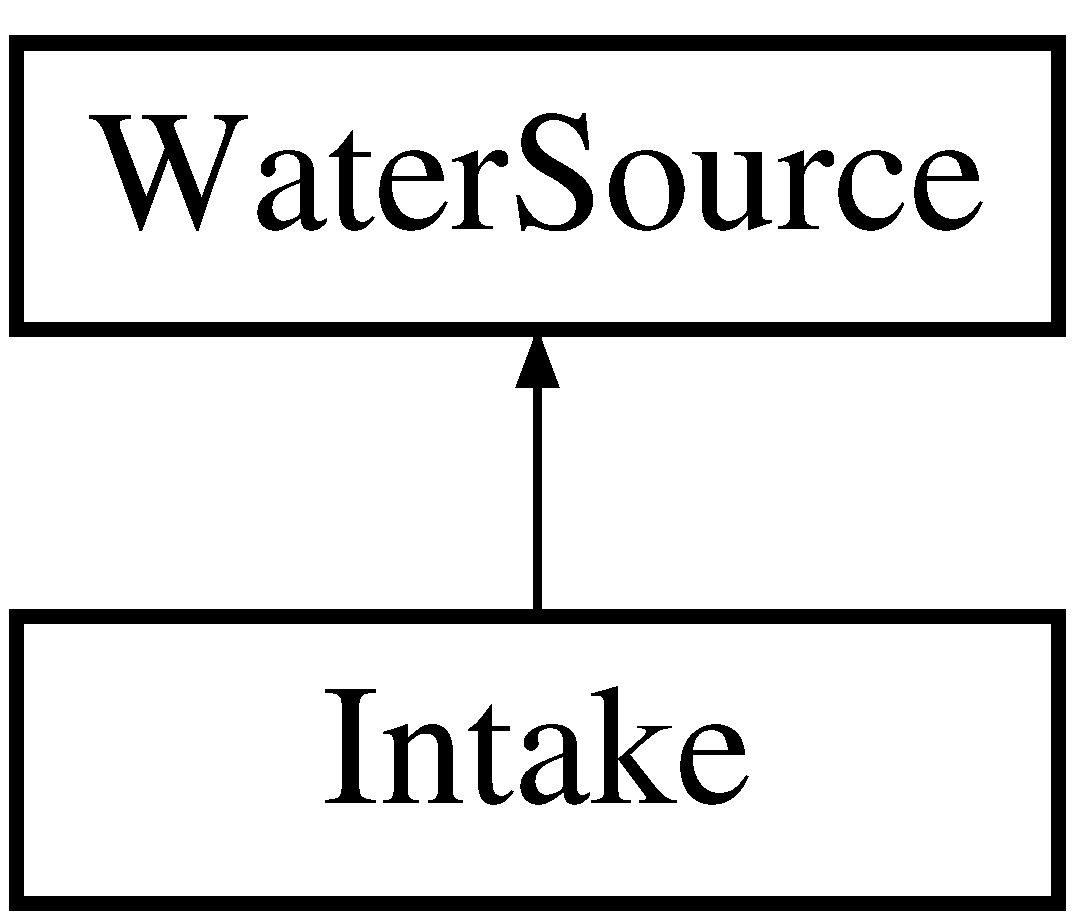
\includegraphics[height=2.000000cm]{classIntake}
\end{center}
\end{figure}
\subsection*{Public Member Functions}
\begin{DoxyCompactItemize}
\item 
\mbox{\hyperlink{classIntake_a02e01801fcaede46e960d497e60eb335}{Intake}} (const char $\ast$\mbox{\hyperlink{classWaterSource_a846ea74c5b453d014f594d41fee8c765}{name}}, const int \mbox{\hyperlink{classWaterSource_a6eafe5dfefd317877d1244e8a7c6e742}{id}}, const vector$<$ \mbox{\hyperlink{classCatchment}{Catchment}} $\ast$$>$ \&\mbox{\hyperlink{classWaterSource_a8c18c34f23f8a06685c1d12f462ed830}{catchments}}, const double max\+\_\+treatment\+\_\+capacity)
\begin{DoxyCompactList}\small\item\em Constructs an \mbox{\hyperlink{classIntake}{Intake}} object with the specified properties. \end{DoxyCompactList}\item 
\mbox{\hyperlink{classIntake_ada4924f9507f07853feb5cb411d1c336}{Intake}} (const char $\ast$\mbox{\hyperlink{classWaterSource_a846ea74c5b453d014f594d41fee8c765}{name}}, const int \mbox{\hyperlink{classWaterSource_a6eafe5dfefd317877d1244e8a7c6e742}{id}}, const vector$<$ \mbox{\hyperlink{classCatchment}{Catchment}} $\ast$$>$ \&\mbox{\hyperlink{classWaterSource_a8c18c34f23f8a06685c1d12f462ed830}{catchments}}, const double raw\+\_\+water\+\_\+capacity, const double max\+\_\+treatment\+\_\+capacity)
\begin{DoxyCompactList}\small\item\em Constructs an \mbox{\hyperlink{classIntake}{Intake}} object with the specified properties, including raw water capacity. \end{DoxyCompactList}\item 
\mbox{\hyperlink{classIntake_a1f6fbdc6fff65337b70b7ca59f061bb4}{Intake}} (const char $\ast$\mbox{\hyperlink{classWaterSource_a846ea74c5b453d014f594d41fee8c765}{name}}, const int \mbox{\hyperlink{classWaterSource_a6eafe5dfefd317877d1244e8a7c6e742}{id}}, const vector$<$ \mbox{\hyperlink{classCatchment}{Catchment}} $\ast$$>$ \&\mbox{\hyperlink{classWaterSource_a8c18c34f23f8a06685c1d12f462ed830}{catchments}}, vector$<$ int $>$ connected\+\_\+sources, const double raw\+\_\+water\+\_\+main\+\_\+capacity, const vector$<$ double $>$ construction\+\_\+time\+\_\+range, double permitting\+\_\+period, \mbox{\hyperlink{classBond}{Bond}} \&bond)
\begin{DoxyCompactList}\small\item\em Constructor for the \mbox{\hyperlink{classIntake}{Intake}} class. \end{DoxyCompactList}\item 
\mbox{\hyperlink{classIntake_aa81e2e35940482717fa67c33b6acd002}{Intake}} (const \mbox{\hyperlink{classIntake}{Intake}} \&intake)
\begin{DoxyCompactList}\small\item\em Copy constructor for the \mbox{\hyperlink{classIntake}{Intake}} class. \end{DoxyCompactList}\item 
\mbox{\hyperlink{classIntake}{Intake}} \& \mbox{\hyperlink{classIntake_aa4a7adbb8380d091197011d9f1877005}{operator=}} (const \mbox{\hyperlink{classIntake}{Intake}} \&intake)
\begin{DoxyCompactList}\small\item\em Assignment operator for the \mbox{\hyperlink{classIntake}{Intake}} class. \end{DoxyCompactList}\item 
\mbox{\hyperlink{classIntake_abf57ff6edf55f292921fb7838059ad26}{$\sim$\+Intake}} () override
\begin{DoxyCompactList}\small\item\em Destructor for the \mbox{\hyperlink{classIntake}{Intake}} class. \end{DoxyCompactList}\item 
void \mbox{\hyperlink{classIntake_acd5ab74c4091b286e69ecdcc495d83ce}{apply\+Continuity}} (int week, double upstream\+\_\+source\+\_\+min\+\_\+env\+\_\+flow, double \mbox{\hyperlink{classWaterSource_aeb5a2d2d83383a70ca20f3e94635a9c7}{wastewater\+\_\+inflow}}, vector$<$ double $>$ \&demand) override
\begin{DoxyCompactList}\small\item\em Applies continuity to update the water availability and demand for the \mbox{\hyperlink{classIntake}{Intake}} system. \end{DoxyCompactList}\item 
void \mbox{\hyperlink{classIntake_a879c4c780a4d21606e848f57464cf3b6}{set\+Realization}} (unsigned long r, vector$<$ double $>$ \&rdm\+\_\+factors) override
\begin{DoxyCompactList}\small\item\em Sets the realization for the \mbox{\hyperlink{classIntake}{Intake}} system based on random factors. \end{DoxyCompactList}\item 
double \mbox{\hyperlink{classIntake_a8d1fc6855451f3dff1a2f0efcd5da8ee}{get\+Priority\+Source\+Potential\+Volume}} (int utility\+\_\+id) const override
\begin{DoxyCompactList}\small\item\em Gets the potential volume available from the priority source. \end{DoxyCompactList}\end{DoxyCompactItemize}
\subsection*{Public Attributes}
\begin{DoxyCompactItemize}
\item 
double \mbox{\hyperlink{classIntake_a5d28f8899e9d4d61983ad8fdf7d58373}{next\+\_\+upstream\+\_\+catchment\+\_\+inflow}} = 0
\begin{DoxyCompactList}\small\item\em The inflow to the intake from the adjacent upstream catchment. \end{DoxyCompactList}\end{DoxyCompactItemize}
\subsection*{Additional Inherited Members}


\subsection{Constructor \& Destructor Documentation}
\mbox{\Hypertarget{classIntake_a02e01801fcaede46e960d497e60eb335}\label{classIntake_a02e01801fcaede46e960d497e60eb335}} 
\index{Intake@{Intake}!Intake@{Intake}}
\index{Intake@{Intake}!Intake@{Intake}}
\subsubsection{\texorpdfstring{Intake()}{Intake()}\hspace{0.1cm}{\footnotesize\ttfamily [1/4]}}
{\footnotesize\ttfamily Intake\+::\+Intake (\begin{DoxyParamCaption}\item[{const char $\ast$}]{name,  }\item[{const int}]{id,  }\item[{const vector$<$ \mbox{\hyperlink{classCatchment}{Catchment}} $\ast$$>$ \&}]{catchments,  }\item[{const double}]{max\+\_\+treatment\+\_\+capacity }\end{DoxyParamCaption})}



Constructs an \mbox{\hyperlink{classIntake}{Intake}} object with the specified properties. 

This constructor initializes an {\ttfamily \mbox{\hyperlink{classIntake}{Intake}}} object, which represents a water source typically used for the intake of water for treatment. It inherits from the {\ttfamily \mbox{\hyperlink{classWaterSource}{Water\+Source}}} class, setting up the properties of the intake such as name, ID, associated catchments, and maximum treatment capacity.


\begin{DoxyParams}{Parameters}
{\em name} & The name of the intake. \\
\hline
{\em id} & The unique identifier for the intake. \\
\hline
{\em catchments} & A vector of pointers to {\ttfamily \mbox{\hyperlink{classCatchment}{Catchment}}} objects associated with this intake. \\
\hline
{\em max\+\_\+treatment\+\_\+capacity} & The maximum treatment capacity of the intake.\\
\hline
\end{DoxyParams}
\begin{DoxyReturn}{Returns}
A constructed {\ttfamily \mbox{\hyperlink{classIntake}{Intake}}} object with the provided properties. 
\end{DoxyReturn}
\mbox{\Hypertarget{classIntake_ada4924f9507f07853feb5cb411d1c336}\label{classIntake_ada4924f9507f07853feb5cb411d1c336}} 
\index{Intake@{Intake}!Intake@{Intake}}
\index{Intake@{Intake}!Intake@{Intake}}
\subsubsection{\texorpdfstring{Intake()}{Intake()}\hspace{0.1cm}{\footnotesize\ttfamily [2/4]}}
{\footnotesize\ttfamily Intake\+::\+Intake (\begin{DoxyParamCaption}\item[{const char $\ast$}]{name,  }\item[{const int}]{id,  }\item[{const vector$<$ \mbox{\hyperlink{classCatchment}{Catchment}} $\ast$$>$ \&}]{catchments,  }\item[{const double}]{raw\+\_\+water\+\_\+capacity,  }\item[{const double}]{max\+\_\+treatment\+\_\+capacity }\end{DoxyParamCaption})}



Constructs an \mbox{\hyperlink{classIntake}{Intake}} object with the specified properties, including raw water capacity. 

This constructor initializes an {\ttfamily \mbox{\hyperlink{classIntake}{Intake}}} object, which represents a water source typically used for the intake of raw water for treatment. It inherits from the {\ttfamily \mbox{\hyperlink{classWaterSource}{Water\+Source}}} class, setting up the properties of the intake such as name, ID, associated catchments, raw water capacity, and maximum treatment capacity.


\begin{DoxyParams}{Parameters}
{\em name} & The name of the intake. \\
\hline
{\em id} & The unique identifier for the intake. \\
\hline
{\em catchments} & A vector of pointers to {\ttfamily \mbox{\hyperlink{classCatchment}{Catchment}}} objects associated with this intake. \\
\hline
{\em raw\+\_\+water\+\_\+capacity} & The raw water intake capacity of the intake. \\
\hline
{\em max\+\_\+treatment\+\_\+capacity} & The maximum treatment capacity of the intake.\\
\hline
\end{DoxyParams}
\begin{DoxyReturn}{Returns}
A constructed {\ttfamily \mbox{\hyperlink{classIntake}{Intake}}} object with the provided properties. 
\end{DoxyReturn}
\mbox{\Hypertarget{classIntake_a1f6fbdc6fff65337b70b7ca59f061bb4}\label{classIntake_a1f6fbdc6fff65337b70b7ca59f061bb4}} 
\index{Intake@{Intake}!Intake@{Intake}}
\index{Intake@{Intake}!Intake@{Intake}}
\subsubsection{\texorpdfstring{Intake()}{Intake()}\hspace{0.1cm}{\footnotesize\ttfamily [3/4]}}
{\footnotesize\ttfamily Intake\+::\+Intake (\begin{DoxyParamCaption}\item[{const char $\ast$}]{name,  }\item[{const int}]{id,  }\item[{const vector$<$ \mbox{\hyperlink{classCatchment}{Catchment}} $\ast$$>$ \&}]{catchments,  }\item[{vector$<$ int $>$}]{connected\+\_\+sources,  }\item[{const double}]{raw\+\_\+water\+\_\+main\+\_\+capacity,  }\item[{const vector$<$ double $>$}]{construction\+\_\+time\+\_\+range,  }\item[{double}]{permitting\+\_\+period,  }\item[{\mbox{\hyperlink{classBond}{Bond}} \&}]{bond }\end{DoxyParamCaption})}



Constructor for the \mbox{\hyperlink{classIntake}{Intake}} class. 

This function initializes the \mbox{\hyperlink{classIntake}{Intake}} class with the details on construction, permitting, and financing.


\begin{DoxyParams}{Parameters}
{\em name} & The name of the intake. \\
\hline
{\em id} & The ID of the intake. \\
\hline
{\em catchments} & A vector of \mbox{\hyperlink{classCatchment}{Catchment}} objects associated with this intake. \\
\hline
{\em connected\+\_\+sources} & A vector of integers representing the connected water sources. \\
\hline
{\em raw\+\_\+water\+\_\+main\+\_\+capacity} & The capacity for raw water intake. \\
\hline
{\em construction\+\_\+time\+\_\+range} & A vector containing the time range for construction. \\
\hline
{\em permitting\+\_\+period} & The permitting period for the intake. \\
\hline
{\em bond} & The \mbox{\hyperlink{classBond}{Bond}} object associated with the intake.\\
\hline
\end{DoxyParams}
\begin{DoxyReturn}{Returns}
A new instance of the \mbox{\hyperlink{classIntake}{Intake}} class initialized with the provided values. 
\end{DoxyReturn}
\mbox{\Hypertarget{classIntake_aa81e2e35940482717fa67c33b6acd002}\label{classIntake_aa81e2e35940482717fa67c33b6acd002}} 
\index{Intake@{Intake}!Intake@{Intake}}
\index{Intake@{Intake}!Intake@{Intake}}
\subsubsection{\texorpdfstring{Intake()}{Intake()}\hspace{0.1cm}{\footnotesize\ttfamily [4/4]}}
{\footnotesize\ttfamily Intake\+::\+Intake (\begin{DoxyParamCaption}\item[{const \mbox{\hyperlink{classIntake}{Intake}} \&}]{intake }\end{DoxyParamCaption})}



Copy constructor for the \mbox{\hyperlink{classIntake}{Intake}} class. 

This constructor initializes a new \mbox{\hyperlink{classIntake}{Intake}} object as a copy of an existing \mbox{\hyperlink{classIntake}{Intake}} object.


\begin{DoxyParams}{Parameters}
{\em intake} & The \mbox{\hyperlink{classIntake}{Intake}} object to copy.\\
\hline
\end{DoxyParams}
\begin{DoxyReturn}{Returns}
A new instance of the \mbox{\hyperlink{classIntake}{Intake}} class that is a copy of the provided \mbox{\hyperlink{classIntake}{Intake}}. 
\end{DoxyReturn}
\mbox{\Hypertarget{classIntake_abf57ff6edf55f292921fb7838059ad26}\label{classIntake_abf57ff6edf55f292921fb7838059ad26}} 
\index{Intake@{Intake}!````~Intake@{$\sim$\+Intake}}
\index{````~Intake@{$\sim$\+Intake}!Intake@{Intake}}
\subsubsection{\texorpdfstring{$\sim$\+Intake()}{~Intake()}}
{\footnotesize\ttfamily Intake\+::$\sim$\+Intake (\begin{DoxyParamCaption}{ }\end{DoxyParamCaption})\hspace{0.3cm}{\ttfamily [override]}}



Destructor for the \mbox{\hyperlink{classIntake}{Intake}} class. 

This destructor clears the list of catchments associated with the \mbox{\hyperlink{classIntake}{Intake}} object. This destructor overrides the default destructor for the \mbox{\hyperlink{classWaterSource}{Water\+Source}} class.

\begin{DoxyReturn}{Returns}
None 
\end{DoxyReturn}


\subsection{Member Function Documentation}
\mbox{\Hypertarget{classIntake_acd5ab74c4091b286e69ecdcc495d83ce}\label{classIntake_acd5ab74c4091b286e69ecdcc495d83ce}} 
\index{Intake@{Intake}!apply\+Continuity@{apply\+Continuity}}
\index{apply\+Continuity@{apply\+Continuity}!Intake@{Intake}}
\subsubsection{\texorpdfstring{apply\+Continuity()}{applyContinuity()}}
{\footnotesize\ttfamily void Intake\+::apply\+Continuity (\begin{DoxyParamCaption}\item[{int}]{week,  }\item[{double}]{upstream\+\_\+source\+\_\+min\+\_\+env\+\_\+flow,  }\item[{double}]{wastewater\+\_\+inflow,  }\item[{vector$<$ double $>$ \&}]{demand }\end{DoxyParamCaption})\hspace{0.3cm}{\ttfamily [override]}, {\ttfamily [virtual]}}



Applies continuity to update the water availability and demand for the \mbox{\hyperlink{classIntake}{Intake}} system. 

This function calculates the total upstream inflow, downstream demand, and the water availability for the next time step. It also computes the total outflow based on the given upstream source inflow, wastewater inflow, and demand outflow. This function overrides the apply\+Continuity function in the \mbox{\hyperlink{classWaterSource}{Water\+Source}} class.

F\+I\+X\+ME\+: W\+H\+EN I\+M\+P\+L\+E\+M\+E\+N\+T\+I\+NG R\+E\+S\+E\+R\+V\+O\+IR R\+U\+L\+ES, A\+DD A \char`\"{}\+B\+A\+N\+K\char`\"{} OF W\+A\+T\+ER O\+V\+ER A\+ND U\+N\+D\+E\+R\+U\+SE TO BE A\+D\+D\+E\+D/\+S\+U\+B\+T\+R\+A\+C\+T\+ED F\+R\+OM T\+HE A\+V\+A\+I\+L\+A\+B\+LE V\+O\+L\+U\+ME F\+OR T\+HE N\+E\+XT R\+E\+A\+L\+I\+Z\+A\+T\+I\+ON.


\begin{DoxyParams}{Parameters}
{\em week} & The current week for which continuity is being applied. \\
\hline
{\em upstream\+\_\+source\+\_\+inflow} & The upstream source inflow during the current week. \\
\hline
{\em wastewater\+\_\+inflow} & The wastewater inflow during the current week. \\
\hline
{\em demand} & The demand for water for each connected utility or system during the current week.\\
\hline
\end{DoxyParams}
\begin{DoxyReturn}{Returns}
None 
\end{DoxyReturn}


Implements \mbox{\hyperlink{classWaterSource_ac070445379fe706f65b977dade4f3fbc}{Water\+Source}}.

\mbox{\Hypertarget{classIntake_a8d1fc6855451f3dff1a2f0efcd5da8ee}\label{classIntake_a8d1fc6855451f3dff1a2f0efcd5da8ee}} 
\index{Intake@{Intake}!get\+Priority\+Source\+Potential\+Volume@{get\+Priority\+Source\+Potential\+Volume}}
\index{get\+Priority\+Source\+Potential\+Volume@{get\+Priority\+Source\+Potential\+Volume}!Intake@{Intake}}
\subsubsection{\texorpdfstring{get\+Priority\+Source\+Potential\+Volume()}{getPrioritySourcePotentialVolume()}}
{\footnotesize\ttfamily double Intake\+::get\+Priority\+Source\+Potential\+Volume (\begin{DoxyParamCaption}\item[{int}]{utility\+\_\+id }\end{DoxyParamCaption}) const\hspace{0.3cm}{\ttfamily [override]}, {\ttfamily [virtual]}}



Gets the potential volume available from the priority source. 

This function calculates the remaining \char`\"{}storage\char`\"{} capacity after accounting for weekly demands and environmental flows. The volume is based on the treatment capacity and inflows. This function overrides the get\+Priority\+Source\+Potential\+Volume function in the \mbox{\hyperlink{classWaterSource}{Water\+Source}} class.


\begin{DoxyParams}{Parameters}
{\em utility\+\_\+id} & The utility identifier. Currently unused in this method but kept for consistency.\\
\hline
\end{DoxyParams}
\begin{DoxyReturn}{Returns}
The remaining potential volume available from the priority source. 
\end{DoxyReturn}


Reimplemented from \mbox{\hyperlink{classWaterSource_a00a432eba75eaae7195338a8514ac853}{Water\+Source}}.

\mbox{\Hypertarget{classIntake_aa4a7adbb8380d091197011d9f1877005}\label{classIntake_aa4a7adbb8380d091197011d9f1877005}} 
\index{Intake@{Intake}!operator=@{operator=}}
\index{operator=@{operator=}!Intake@{Intake}}
\subsubsection{\texorpdfstring{operator=()}{operator=()}}
{\footnotesize\ttfamily \mbox{\hyperlink{classIntake}{Intake}}\& Intake\+::operator= (\begin{DoxyParamCaption}\item[{const \mbox{\hyperlink{classIntake}{Intake}} \&}]{intake }\end{DoxyParamCaption})}



Assignment operator for the \mbox{\hyperlink{classIntake}{Intake}} class. 

This operator assigns the values of an existing \mbox{\hyperlink{classIntake}{Intake}} object to the current object.


\begin{DoxyParams}{Parameters}
{\em intake} & The \mbox{\hyperlink{classIntake}{Intake}} object to assign from.\\
\hline
\end{DoxyParams}
\begin{DoxyReturn}{Returns}
A reference to the current \mbox{\hyperlink{classIntake}{Intake}} object after the assignment. 
\end{DoxyReturn}
\mbox{\Hypertarget{classIntake_a879c4c780a4d21606e848f57464cf3b6}\label{classIntake_a879c4c780a4d21606e848f57464cf3b6}} 
\index{Intake@{Intake}!set\+Realization@{set\+Realization}}
\index{set\+Realization@{set\+Realization}!Intake@{Intake}}
\subsubsection{\texorpdfstring{set\+Realization()}{setRealization()}}
{\footnotesize\ttfamily void Intake\+::set\+Realization (\begin{DoxyParamCaption}\item[{unsigned long}]{r,  }\item[{vector$<$ double $>$ \&}]{rdm\+\_\+factors }\end{DoxyParamCaption})\hspace{0.3cm}{\ttfamily [override]}, {\ttfamily [virtual]}}



Sets the realization for the \mbox{\hyperlink{classIntake}{Intake}} system based on random factors. 

This function updates the total demand and available volume for the \mbox{\hyperlink{classIntake}{Intake}} system based on a new realization and corresponding random factors. Thid function overrides the set\+Realization function in the \mbox{\hyperlink{classWaterSource}{Water\+Source}} class.


\begin{DoxyParams}{Parameters}
{\em r} & The realization index, used to set the state for the given realization. \\
\hline
{\em rdm\+\_\+factors} & The random factors that influence the realization.\\
\hline
\end{DoxyParams}
\begin{DoxyReturn}{Returns}
None 
\end{DoxyReturn}


Reimplemented from \mbox{\hyperlink{classWaterSource_a634904c510b16de6d7c057fed6d6e625}{Water\+Source}}.



\subsection{Member Data Documentation}
\mbox{\Hypertarget{classIntake_a5d28f8899e9d4d61983ad8fdf7d58373}\label{classIntake_a5d28f8899e9d4d61983ad8fdf7d58373}} 
\index{Intake@{Intake}!next\+\_\+upstream\+\_\+catchment\+\_\+inflow@{next\+\_\+upstream\+\_\+catchment\+\_\+inflow}}
\index{next\+\_\+upstream\+\_\+catchment\+\_\+inflow@{next\+\_\+upstream\+\_\+catchment\+\_\+inflow}!Intake@{Intake}}
\subsubsection{\texorpdfstring{next\+\_\+upstream\+\_\+catchment\+\_\+inflow}{next\_upstream\_catchment\_inflow}}
{\footnotesize\ttfamily double Intake\+::next\+\_\+upstream\+\_\+catchment\+\_\+inflow = 0}



The inflow to the intake from the adjacent upstream catchment. 



The documentation for this class was generated from the following file\+:\begin{DoxyCompactItemize}
\item 
/home/fs02/pmr82\+\_\+0001/lbl59/\+Water\+Paths-\/doc/src/\+System\+Components/\+Water\+Sources/\mbox{\hyperlink{Intake_8h}{Intake.\+h}}\end{DoxyCompactItemize}

\hypertarget{classIntakeExpansion}{}\section{Intake\+Expansion Class Reference}
\label{classIntakeExpansion}\index{Intake\+Expansion@{Intake\+Expansion}}


{\ttfamily \#include $<$Intake\+Expansion.\+h$>$}

Inheritance diagram for Intake\+Expansion\+:\begin{figure}[H]
\begin{center}
\leavevmode
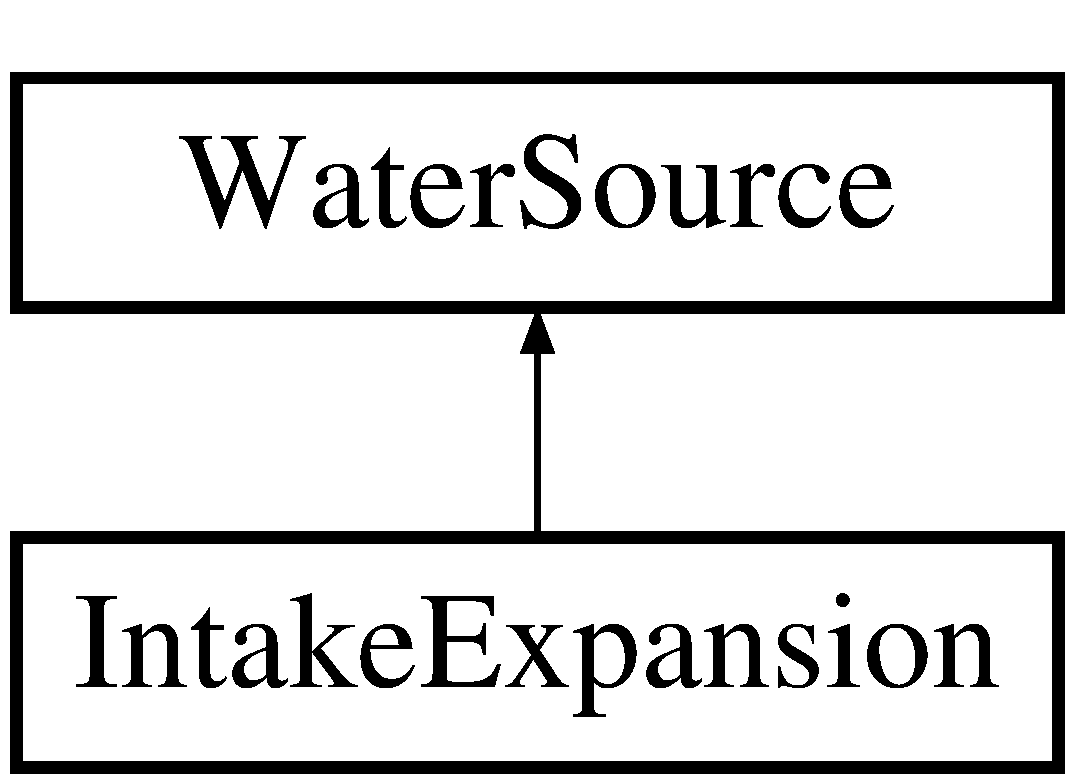
\includegraphics[height=2.000000cm]{classIntakeExpansion}
\end{center}
\end{figure}
\subsection*{Public Member Functions}
\begin{DoxyCompactItemize}
\item 
\mbox{\hyperlink{classIntakeExpansion_abf871880367036c599caab901eb46339}{Intake\+Expansion}} (const char $\ast$\mbox{\hyperlink{classWaterSource_a846ea74c5b453d014f594d41fee8c765}{name}}, const int \mbox{\hyperlink{classWaterSource_a6eafe5dfefd317877d1244e8a7c6e742}{id}}, const unsigned int \mbox{\hyperlink{classIntakeExpansion_a93569405968a66226046e730e691615c}{parent\+\_\+intake\+\_\+\+ID}}, const double capacity\+\_\+added, const double treatment\+\_\+capacity\+\_\+added, const vector$<$ double $>$ \&construction\+\_\+time\+\_\+range, vector$<$ int $>$ connected\+\_\+sources, double permitting\+\_\+period, \mbox{\hyperlink{classBond}{Bond}} \&bond)
\begin{DoxyCompactList}\small\item\em Constructs an \mbox{\hyperlink{classIntakeExpansion}{Intake\+Expansion}} object. \end{DoxyCompactList}\item 
\mbox{\hyperlink{classIntakeExpansion_a88a12d71e8c3bcba51de9f21636f866f}{Intake\+Expansion}} (const \mbox{\hyperlink{classIntakeExpansion}{Intake\+Expansion}} \&intake\+\_\+expansion)
\begin{DoxyCompactList}\small\item\em Copy constructor for the \mbox{\hyperlink{classIntakeExpansion}{Intake\+Expansion}} class. \end{DoxyCompactList}\item 
\mbox{\hyperlink{classIntakeExpansion}{Intake\+Expansion}} \& \mbox{\hyperlink{classIntakeExpansion_a554bef7ab4c9216147baa9df5c35d17e}{operator=}} (const \mbox{\hyperlink{classIntakeExpansion}{Intake\+Expansion}} \&intake\+\_\+expansion)
\begin{DoxyCompactList}\small\item\em Assignment operator for the \mbox{\hyperlink{classIntakeExpansion}{Intake\+Expansion}} class. \end{DoxyCompactList}\item 
void \mbox{\hyperlink{classIntakeExpansion_a8686b58c65444182ba19b783fc6ff77f}{apply\+Continuity}} (int week, double \mbox{\hyperlink{classWaterSource_a7a69b2e9b6030f1035e6cf44d2918ee5}{upstream\+\_\+source\+\_\+inflow}}, double wastewater\+\_\+discharge, vector$<$ double $>$ \&demand\+\_\+outflow) override
\begin{DoxyCompactList}\small\item\em Applies continuity for the \mbox{\hyperlink{classIntakeExpansion}{Intake\+Expansion}} class. \end{DoxyCompactList}\end{DoxyCompactItemize}
\subsection*{Public Attributes}
\begin{DoxyCompactItemize}
\item 
const unsigned int \mbox{\hyperlink{classIntakeExpansion_a93569405968a66226046e730e691615c}{parent\+\_\+intake\+\_\+\+ID}}
\begin{DoxyCompactList}\small\item\em The ID of the parent intake. \end{DoxyCompactList}\end{DoxyCompactItemize}
\subsection*{Additional Inherited Members}


\subsection{Constructor \& Destructor Documentation}
\mbox{\Hypertarget{classIntakeExpansion_abf871880367036c599caab901eb46339}\label{classIntakeExpansion_abf871880367036c599caab901eb46339}} 
\index{Intake\+Expansion@{Intake\+Expansion}!Intake\+Expansion@{Intake\+Expansion}}
\index{Intake\+Expansion@{Intake\+Expansion}!Intake\+Expansion@{Intake\+Expansion}}
\subsubsection{\texorpdfstring{Intake\+Expansion()}{IntakeExpansion()}\hspace{0.1cm}{\footnotesize\ttfamily [1/2]}}
{\footnotesize\ttfamily Intake\+Expansion\+::\+Intake\+Expansion (\begin{DoxyParamCaption}\item[{const char $\ast$}]{name,  }\item[{const int}]{id,  }\item[{const unsigned int}]{parent\+\_\+intake\+\_\+\+ID,  }\item[{const double}]{capacity\+\_\+added,  }\item[{const double}]{treatment\+\_\+capacity\+\_\+added,  }\item[{const vector$<$ double $>$ \&}]{construction\+\_\+time\+\_\+range,  }\item[{vector$<$ int $>$}]{connected\+\_\+sources,  }\item[{double}]{permitting\+\_\+period,  }\item[{\mbox{\hyperlink{classBond}{Bond}} \&}]{bond }\end{DoxyParamCaption})}



Constructs an \mbox{\hyperlink{classIntakeExpansion}{Intake\+Expansion}} object. 

This constructor initializes the \mbox{\hyperlink{classIntakeExpansion}{Intake\+Expansion}} object, which represents the expansion of an existing intake system by adding extra capacity and treatment capacity.


\begin{DoxyParams}{Parameters}
{\em name} & The name of the intake expansion. \\
\hline
{\em id} & The unique identifier for the intake expansion. \\
\hline
{\em parent\+\_\+intake\+\_\+\+ID} & The ID of the parent intake from which this expansion is derived. \\
\hline
{\em capacity\+\_\+added} & The additional capacity added to the intake. \\
\hline
{\em treatment\+\_\+capacity\+\_\+added} & The additional treatment capacity added to the intake. \\
\hline
{\em construction\+\_\+time\+\_\+range} & The time range for the construction of the expansion. \\
\hline
{\em connected\+\_\+sources} & The list of connected sources to the intake expansion. \\
\hline
{\em permitting\+\_\+period} & The permitting period for the expansion. \\
\hline
{\em bond} & The bond associated with the intake expansion.\\
\hline
\end{DoxyParams}
\begin{DoxyReturn}{Returns}
A new \mbox{\hyperlink{classIntakeExpansion}{Intake\+Expansion}} object. 
\end{DoxyReturn}
\mbox{\Hypertarget{classIntakeExpansion_a88a12d71e8c3bcba51de9f21636f866f}\label{classIntakeExpansion_a88a12d71e8c3bcba51de9f21636f866f}} 
\index{Intake\+Expansion@{Intake\+Expansion}!Intake\+Expansion@{Intake\+Expansion}}
\index{Intake\+Expansion@{Intake\+Expansion}!Intake\+Expansion@{Intake\+Expansion}}
\subsubsection{\texorpdfstring{Intake\+Expansion()}{IntakeExpansion()}\hspace{0.1cm}{\footnotesize\ttfamily [2/2]}}
{\footnotesize\ttfamily Intake\+Expansion\+::\+Intake\+Expansion (\begin{DoxyParamCaption}\item[{const \mbox{\hyperlink{classIntakeExpansion}{Intake\+Expansion}} \&}]{intake\+\_\+expansion }\end{DoxyParamCaption})}



Copy constructor for the \mbox{\hyperlink{classIntakeExpansion}{Intake\+Expansion}} class. 

This constructor creates a new {\ttfamily \mbox{\hyperlink{classIntakeExpansion}{Intake\+Expansion}}} object by copying the properties of an existing one. It ensures that both the {\ttfamily \mbox{\hyperlink{classWaterSource}{Water\+Source}}} and {\ttfamily parent\+\_\+intake\+\_\+\+ID} are properly copied.


\begin{DoxyParams}{Parameters}
{\em intake\+\_\+expansion} & The {\ttfamily \mbox{\hyperlink{classIntakeExpansion}{Intake\+Expansion}}} object to copy.\\
\hline
\end{DoxyParams}
\begin{DoxyReturn}{Returns}
A new {\ttfamily \mbox{\hyperlink{classIntakeExpansion}{Intake\+Expansion}}} object with the same properties as {\ttfamily intake\+\_\+expansion}. 
\end{DoxyReturn}


\subsection{Member Function Documentation}
\mbox{\Hypertarget{classIntakeExpansion_a8686b58c65444182ba19b783fc6ff77f}\label{classIntakeExpansion_a8686b58c65444182ba19b783fc6ff77f}} 
\index{Intake\+Expansion@{Intake\+Expansion}!apply\+Continuity@{apply\+Continuity}}
\index{apply\+Continuity@{apply\+Continuity}!Intake\+Expansion@{Intake\+Expansion}}
\subsubsection{\texorpdfstring{apply\+Continuity()}{applyContinuity()}}
{\footnotesize\ttfamily void Intake\+Expansion\+::apply\+Continuity (\begin{DoxyParamCaption}\item[{int}]{week,  }\item[{double}]{upstream\+\_\+source\+\_\+inflow,  }\item[{double}]{wastewater\+\_\+discharge,  }\item[{vector$<$ double $>$ \&}]{demand\+\_\+outflow }\end{DoxyParamCaption})\hspace{0.3cm}{\ttfamily [override]}, {\ttfamily [virtual]}}



Applies continuity for the \mbox{\hyperlink{classIntakeExpansion}{Intake\+Expansion}} class. 

This function applies the continuity equation for the intake expansion process. This function does not have a specific implementation, taking on the behavior from the parent {\ttfamily \mbox{\hyperlink{classWaterSource}{Water\+Source}}} class.


\begin{DoxyParams}{Parameters}
{\em week} & The current week for which continuity is applied. \\
\hline
{\em upstream\+\_\+source\+\_\+inflow} & The inflow from upstream sources. \\
\hline
{\em wastewater\+\_\+discharge} & The discharge from wastewater sources. \\
\hline
{\em demand\+\_\+outflow} & A vector containing the outflows of water demands.\\
\hline
\end{DoxyParams}
\begin{DoxyReturn}{Returns}
void 
\end{DoxyReturn}


Implements \mbox{\hyperlink{classWaterSource_ac070445379fe706f65b977dade4f3fbc}{Water\+Source}}.

\mbox{\Hypertarget{classIntakeExpansion_a554bef7ab4c9216147baa9df5c35d17e}\label{classIntakeExpansion_a554bef7ab4c9216147baa9df5c35d17e}} 
\index{Intake\+Expansion@{Intake\+Expansion}!operator=@{operator=}}
\index{operator=@{operator=}!Intake\+Expansion@{Intake\+Expansion}}
\subsubsection{\texorpdfstring{operator=()}{operator=()}}
{\footnotesize\ttfamily \mbox{\hyperlink{classIntakeExpansion}{Intake\+Expansion}}\& Intake\+Expansion\+::operator= (\begin{DoxyParamCaption}\item[{const \mbox{\hyperlink{classIntakeExpansion}{Intake\+Expansion}} \&}]{intake\+\_\+expansion }\end{DoxyParamCaption})}



Assignment operator for the \mbox{\hyperlink{classIntakeExpansion}{Intake\+Expansion}} class. 

This operator assigns the properties of one {\ttfamily \mbox{\hyperlink{classIntakeExpansion}{Intake\+Expansion}}} object to another. It ensures that both the {\ttfamily \mbox{\hyperlink{classWaterSource}{Water\+Source}}} and {\ttfamily parent\+\_\+intake\+\_\+\+ID} are correctly assigned.


\begin{DoxyParams}{Parameters}
{\em intake\+\_\+expansion} & The {\ttfamily \mbox{\hyperlink{classIntakeExpansion}{Intake\+Expansion}}} object to assign from.\\
\hline
\end{DoxyParams}
\begin{DoxyReturn}{Returns}
A reference to the current {\ttfamily \mbox{\hyperlink{classIntakeExpansion}{Intake\+Expansion}}} object after the assignment. 
\end{DoxyReturn}


\subsection{Member Data Documentation}
\mbox{\Hypertarget{classIntakeExpansion_a93569405968a66226046e730e691615c}\label{classIntakeExpansion_a93569405968a66226046e730e691615c}} 
\index{Intake\+Expansion@{Intake\+Expansion}!parent\+\_\+intake\+\_\+\+ID@{parent\+\_\+intake\+\_\+\+ID}}
\index{parent\+\_\+intake\+\_\+\+ID@{parent\+\_\+intake\+\_\+\+ID}!Intake\+Expansion@{Intake\+Expansion}}
\subsubsection{\texorpdfstring{parent\+\_\+intake\+\_\+\+ID}{parent\_intake\_ID}}
{\footnotesize\ttfamily const unsigned int Intake\+Expansion\+::parent\+\_\+intake\+\_\+\+ID}



The ID of the parent intake. 



The documentation for this class was generated from the following file\+:\begin{DoxyCompactItemize}
\item 
/home/fs02/pmr82\+\_\+0001/lbl59/\+Water\+Paths-\/doc/src/\+System\+Components/\+Water\+Sources/\mbox{\hyperlink{IntakeExpansion_8h}{Intake\+Expansion.\+h}}\end{DoxyCompactItemize}

\hypertarget{classJointWTP}{}\section{Joint\+W\+TP Class Reference}
\label{classJointWTP}\index{Joint\+W\+TP@{Joint\+W\+TP}}


{\ttfamily \#include $<$Joint\+W\+T\+P.\+h$>$}

Inheritance diagram for Joint\+W\+TP\+:\begin{figure}[H]
\begin{center}
\leavevmode
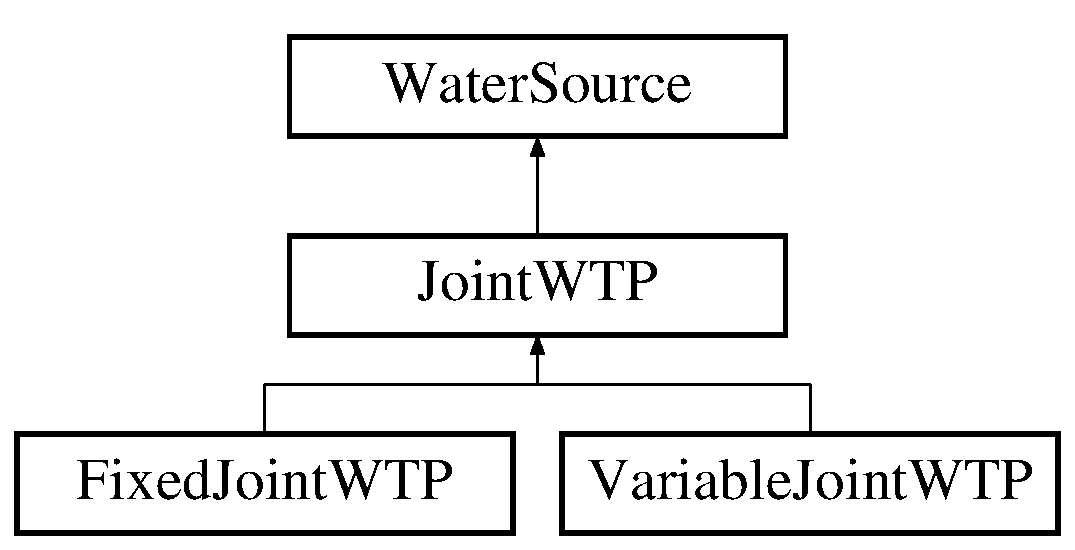
\includegraphics[height=3.000000cm]{classJointWTP}
\end{center}
\end{figure}
\subsection*{Public Member Functions}
\begin{DoxyCompactItemize}
\item 
\mbox{\hyperlink{classJointWTP_a1aeeff203eb631ca3bfcf407ab0bbd4f}{Joint\+W\+TP}} (const char $\ast$\mbox{\hyperlink{classWaterSource_a846ea74c5b453d014f594d41fee8c765}{name}}, const int \mbox{\hyperlink{classWaterSource_a6eafe5dfefd317877d1244e8a7c6e742}{id}}, const int agreement\+\_\+type, const int \mbox{\hyperlink{classJointWTP_aa5830cb4d3013a004b7168f4dbf475eb}{parent\+\_\+reservoir\+\_\+\+ID}}, const int \mbox{\hyperlink{classJointWTP_a0e10a7f7ade04d5f3572f185de1b8653}{expansion\+\_\+sequence\+\_\+id}}, const double \mbox{\hyperlink{classWaterSource_a2fdfd5ff7d103e71108cf2a31babaccb}{total\+\_\+treatment\+\_\+capacity}}, vector$<$ int $>$ connected\+\_\+sources, vector$<$ int $>$ \&agreement\+\_\+utility\+\_\+ids, vector$<$ double $>$ \&agreement\+\_\+utility\+\_\+treatment\+\_\+capacities, vector$<$ \mbox{\hyperlink{classBond}{Bond}} $\ast$$>$ \&\mbox{\hyperlink{classWaterSource_a413b094e11bdce62f4d82e5bb9e4706e}{bonds}}, const vector$<$ double $>$ \&construction\+\_\+time\+\_\+range, double permitting\+\_\+period)
\begin{DoxyCompactList}\small\item\em Constructor for the \mbox{\hyperlink{classJointWTP}{Joint\+W\+TP}} class. \end{DoxyCompactList}\item 
\mbox{\hyperlink{classJointWTP_a8b3f000183e4e070bcfc9c20f4be9b54}{Joint\+W\+TP}} (const \mbox{\hyperlink{classJointWTP}{Joint\+W\+TP}} \&joint\+\_\+water\+\_\+treatment\+\_\+plant)
\begin{DoxyCompactList}\small\item\em Copy constructor for the \mbox{\hyperlink{classJointWTP}{Joint\+W\+TP}} class. \end{DoxyCompactList}\item 
\mbox{\hyperlink{classJointWTP_aa4abdd96213a3c9d1b286f75eadcef1f}{$\sim$\+Joint\+W\+TP}} () override
\begin{DoxyCompactList}\small\item\em Destructor for the \mbox{\hyperlink{classJointWTP}{Joint\+W\+TP}} class. \end{DoxyCompactList}\item 
\mbox{\hyperlink{classJointWTP}{Joint\+W\+TP}} \& \mbox{\hyperlink{classJointWTP_a00f348852618d93725c6c83bac49bf00}{operator=}} (const \mbox{\hyperlink{classJointWTP}{Joint\+W\+TP}} \&joint\+\_\+water\+\_\+treatment\+\_\+plant)
\begin{DoxyCompactList}\small\item\em Assignment operator for the \mbox{\hyperlink{classJointWTP}{Joint\+W\+TP}} class. \end{DoxyCompactList}\item 
void \mbox{\hyperlink{classJointWTP_a07106b573ea34386621a95d3fbcafd1a}{apply\+Continuity}} (int week, double \mbox{\hyperlink{classWaterSource_a7a69b2e9b6030f1035e6cf44d2918ee5}{upstream\+\_\+source\+\_\+inflow}}, double wastewater\+\_\+discharge, vector$<$ double $>$ \&demand\+\_\+outflow) override
\begin{DoxyCompactList}\small\item\em Applies continuity for the \mbox{\hyperlink{classJointWTP}{Joint\+W\+TP}} class. \end{DoxyCompactList}\item 
virtual double \mbox{\hyperlink{classJointWTP_ae8a2a5c4d5173b43d30fc9c1169574f8}{implement\+Initial\+Treatment\+Capacity}} (int utility\+\_\+id)
\begin{DoxyCompactList}\small\item\em Implements the initial treatment capacity for the \mbox{\hyperlink{classJointWTP}{Joint\+W\+TP}} class. \end{DoxyCompactList}\item 
int \mbox{\hyperlink{classJointWTP_a4580529f08f6499def6aae2655484e48}{get\+Agreement\+Type}} () const override
\begin{DoxyCompactList}\small\item\em Retrieves the agreement type of the \mbox{\hyperlink{classJointWTP}{Joint\+W\+TP}}. \end{DoxyCompactList}\item 
int \mbox{\hyperlink{classJointWTP_ae4805e616725c109f23c0513d6ef2711}{get\+Parent\+Water\+Source\+ID}} () const override
\begin{DoxyCompactList}\small\item\em Retrieves the parent reservoir ID associated with the \mbox{\hyperlink{classJointWTP}{Joint\+W\+TP}}. \end{DoxyCompactList}\item 
double \mbox{\hyperlink{classJointWTP_a3c661704dec4c92b8c16f28e39ca533e}{get\+Allocated\+Treatment\+Fraction}} (int utility\+\_\+id) const override
\begin{DoxyCompactList}\small\item\em Calculates the allocated treatment fraction for a given utility. \end{DoxyCompactList}\end{DoxyCompactItemize}
\subsection*{Public Attributes}
\begin{DoxyCompactItemize}
\item 
const int \mbox{\hyperlink{classJointWTP_a0e10a7f7ade04d5f3572f185de1b8653}{expansion\+\_\+sequence\+\_\+id}}
\begin{DoxyCompactList}\small\item\em The low or high expansion ID of the \mbox{\hyperlink{classJointWTP}{Joint\+W\+TP}} object. \end{DoxyCompactList}\item 
const unsigned int \mbox{\hyperlink{classJointWTP_aa5830cb4d3013a004b7168f4dbf475eb}{parent\+\_\+reservoir\+\_\+\+ID}}
\begin{DoxyCompactList}\small\item\em The ID of the parent reservoir. \end{DoxyCompactList}\item 
const int \mbox{\hyperlink{classJointWTP_ac5663480c912b1b7cfdfb976b4fa3cec}{joint\+\_\+agreement\+\_\+type}}
\begin{DoxyCompactList}\small\item\em The type of agreement for the \mbox{\hyperlink{classJointWTP}{Joint\+W\+TP}}. \end{DoxyCompactList}\end{DoxyCompactItemize}
\subsection*{Additional Inherited Members}


\subsection{Constructor \& Destructor Documentation}
\mbox{\Hypertarget{classJointWTP_a1aeeff203eb631ca3bfcf407ab0bbd4f}\label{classJointWTP_a1aeeff203eb631ca3bfcf407ab0bbd4f}} 
\index{Joint\+W\+TP@{Joint\+W\+TP}!Joint\+W\+TP@{Joint\+W\+TP}}
\index{Joint\+W\+TP@{Joint\+W\+TP}!Joint\+W\+TP@{Joint\+W\+TP}}
\subsubsection{\texorpdfstring{Joint\+W\+T\+P()}{JointWTP()}\hspace{0.1cm}{\footnotesize\ttfamily [1/2]}}
{\footnotesize\ttfamily Joint\+W\+T\+P\+::\+Joint\+W\+TP (\begin{DoxyParamCaption}\item[{const char $\ast$}]{name,  }\item[{const int}]{id,  }\item[{const int}]{agreement\+\_\+type,  }\item[{const int}]{parent\+\_\+reservoir\+\_\+\+ID,  }\item[{const int}]{expansion\+\_\+sequence\+\_\+id,  }\item[{const double}]{total\+\_\+treatment\+\_\+capacity,  }\item[{vector$<$ int $>$}]{connected\+\_\+sources,  }\item[{vector$<$ int $>$ \&}]{agreement\+\_\+utility\+\_\+ids,  }\item[{vector$<$ double $>$ \&}]{agreement\+\_\+utility\+\_\+treatment\+\_\+capacities,  }\item[{vector$<$ \mbox{\hyperlink{classBond}{Bond}} $\ast$$>$ \&}]{bonds,  }\item[{const vector$<$ double $>$ \&}]{construction\+\_\+time\+\_\+range,  }\item[{double}]{permitting\+\_\+period }\end{DoxyParamCaption})}



Constructor for the \mbox{\hyperlink{classJointWTP}{Joint\+W\+TP}} class. 

This constructor initializes a Joint Water Treatment Plant (W\+TP) with the given parameters, including the name, ID, agreement type, parent reservoir ID, expansion sequence, treatment capacity, connected sources, and various other settings. It also initializes the associated bonds and construction time range.


\begin{DoxyParams}{Parameters}
{\em name} & The name of the \mbox{\hyperlink{classJointWTP}{Joint\+W\+TP}}. \\
\hline
{\em id} & The unique identifier of the \mbox{\hyperlink{classJointWTP}{Joint\+W\+TP}}. \\
\hline
{\em agreement\+\_\+type} & The agreement type for the \mbox{\hyperlink{classJointWTP}{Joint\+W\+TP}} (e.\+g., shared, private). \\
\hline
{\em parent\+\_\+reservoir\+\_\+\+ID} & The ID of the parent reservoir associated with the \mbox{\hyperlink{classJointWTP}{Joint\+W\+TP}}. \\
\hline
{\em expansion\+\_\+sequence\+\_\+id} & The ID that defines the sequence of expansion for the \mbox{\hyperlink{classJointWTP}{Joint\+W\+TP}} (low/high). \\
\hline
{\em total\+\_\+treatment\+\_\+capacity} & The total treatment capacity of the \mbox{\hyperlink{classJointWTP}{Joint\+W\+TP}}. \\
\hline
{\em connected\+\_\+sources} & A vector containing the I\+Ds of sources connected to the \mbox{\hyperlink{classJointWTP}{Joint\+W\+TP}}. \\
\hline
{\em agreement\+\_\+utility\+\_\+ids} & A vector containing the I\+Ds of utilities involved in the agreement. \\
\hline
{\em agreement\+\_\+utility\+\_\+treatment\+\_\+capacities} & A vector containing the treatment capacities allocated to the utilities in the agreement. \\
\hline
{\em bonds} & A vector containing bonds related to the \mbox{\hyperlink{classJointWTP}{Joint\+W\+TP}}. \\
\hline
{\em construction\+\_\+time\+\_\+range} & A vector specifying the construction time range for the \mbox{\hyperlink{classJointWTP}{Joint\+W\+TP}}. \\
\hline
{\em permitting\+\_\+period} & The permitting period for the \mbox{\hyperlink{classJointWTP}{Joint\+W\+TP}}.\\
\hline
\end{DoxyParams}
\begin{DoxyReturn}{Returns}
A new instance of the \mbox{\hyperlink{classJointWTP}{Joint\+W\+TP}} class. 
\end{DoxyReturn}
\mbox{\Hypertarget{classJointWTP_a8b3f000183e4e070bcfc9c20f4be9b54}\label{classJointWTP_a8b3f000183e4e070bcfc9c20f4be9b54}} 
\index{Joint\+W\+TP@{Joint\+W\+TP}!Joint\+W\+TP@{Joint\+W\+TP}}
\index{Joint\+W\+TP@{Joint\+W\+TP}!Joint\+W\+TP@{Joint\+W\+TP}}
\subsubsection{\texorpdfstring{Joint\+W\+T\+P()}{JointWTP()}\hspace{0.1cm}{\footnotesize\ttfamily [2/2]}}
{\footnotesize\ttfamily Joint\+W\+T\+P\+::\+Joint\+W\+TP (\begin{DoxyParamCaption}\item[{const \mbox{\hyperlink{classJointWTP}{Joint\+W\+TP}} \&}]{joint\+\_\+water\+\_\+treatment\+\_\+plant }\end{DoxyParamCaption})}



Copy constructor for the \mbox{\hyperlink{classJointWTP}{Joint\+W\+TP}} class. 

This constructor creates a new instance of the \mbox{\hyperlink{classJointWTP}{Joint\+W\+TP}} class by copying the data from an existing {\ttfamily joint\+\_\+water\+\_\+treatment\+\_\+plant} object. It initializes the new instance by copying the base class ({\ttfamily \mbox{\hyperlink{classWaterSource}{Water\+Source}}}) data and the specific attributes of the {\ttfamily \mbox{\hyperlink{classJointWTP}{Joint\+W\+TP}}} class.


\begin{DoxyParams}{Parameters}
{\em joint\+\_\+water\+\_\+treatment\+\_\+plant} & The \mbox{\hyperlink{classJointWTP}{Joint\+W\+TP}} instance to copy from.\\
\hline
\end{DoxyParams}
\begin{DoxyReturn}{Returns}
A new instance of the \mbox{\hyperlink{classJointWTP}{Joint\+W\+TP}} class, with data copied from the given {\ttfamily joint\+\_\+water\+\_\+treatment\+\_\+plant}. 
\end{DoxyReturn}
\mbox{\Hypertarget{classJointWTP_aa4abdd96213a3c9d1b286f75eadcef1f}\label{classJointWTP_aa4abdd96213a3c9d1b286f75eadcef1f}} 
\index{Joint\+W\+TP@{Joint\+W\+TP}!````~Joint\+W\+TP@{$\sim$\+Joint\+W\+TP}}
\index{````~Joint\+W\+TP@{$\sim$\+Joint\+W\+TP}!Joint\+W\+TP@{Joint\+W\+TP}}
\subsubsection{\texorpdfstring{$\sim$\+Joint\+W\+T\+P()}{~JointWTP()}}
{\footnotesize\ttfamily Joint\+W\+T\+P\+::$\sim$\+Joint\+W\+TP (\begin{DoxyParamCaption}{ }\end{DoxyParamCaption})\hspace{0.3cm}{\ttfamily [override]}}



Destructor for the \mbox{\hyperlink{classJointWTP}{Joint\+W\+TP}} class. 

This destructor is automatically invoked when an instance of the \mbox{\hyperlink{classJointWTP}{Joint\+W\+TP}} class goes out of scope or is deleted. It performs any necessary cleanup, but in this case, the destructor is defaulted and doesn\textquotesingle{}t perform any custom actions.

\begin{DoxyReturn}{Returns}
None 
\end{DoxyReturn}


\subsection{Member Function Documentation}
\mbox{\Hypertarget{classJointWTP_a07106b573ea34386621a95d3fbcafd1a}\label{classJointWTP_a07106b573ea34386621a95d3fbcafd1a}} 
\index{Joint\+W\+TP@{Joint\+W\+TP}!apply\+Continuity@{apply\+Continuity}}
\index{apply\+Continuity@{apply\+Continuity}!Joint\+W\+TP@{Joint\+W\+TP}}
\subsubsection{\texorpdfstring{apply\+Continuity()}{applyContinuity()}}
{\footnotesize\ttfamily void Joint\+W\+T\+P\+::apply\+Continuity (\begin{DoxyParamCaption}\item[{int}]{week,  }\item[{double}]{upstream\+\_\+source\+\_\+inflow,  }\item[{double}]{wastewater\+\_\+discharge,  }\item[{vector$<$ double $>$ \&}]{demand\+\_\+outflow }\end{DoxyParamCaption})\hspace{0.3cm}{\ttfamily [override]}, {\ttfamily [virtual]}}



Applies continuity for the \mbox{\hyperlink{classJointWTP}{Joint\+W\+TP}} class. 

This function is called to apply the continuity of the water treatment process. However, it is not designed to be called on a \mbox{\hyperlink{classJointWTP}{Joint\+W\+TP}} instance. It throws a {\ttfamily logic\+\_\+error} to indicate that continuity should be applied only to the associated reservoir being expanded, not the \mbox{\hyperlink{classJointWTP}{Joint\+W\+TP}} itself. This function overrides the {\ttfamily apply\+Continuity} function in the base class {\ttfamily \mbox{\hyperlink{classWaterSource}{Water\+Source}}}.


\begin{DoxyParams}{Parameters}
{\em week} & The current week in the simulation (used for inflow and outflow calculations). \\
\hline
{\em upstream\+\_\+source\+\_\+inflow} & The volume of water inflow from upstream sources for the given week. \\
\hline
{\em wastewater\+\_\+discharge} & The volume of wastewater being discharged into the system. \\
\hline
{\em demand\+\_\+outflow} & A vector representing the water demand outflow for each utility or demand point.\\
\hline
\end{DoxyParams}
\begin{DoxyReturn}{Returns}
None 
\end{DoxyReturn}

\begin{DoxyExceptions}{Exceptions}
{\em logic\+\_\+error} & If called on a \mbox{\hyperlink{classJointWTP}{Joint\+W\+TP}} instance, throws an error indicating that continuity should be applied to the reservoir being expanded, not the \mbox{\hyperlink{classJointWTP}{Joint\+W\+TP}}. \\
\hline
\end{DoxyExceptions}


Implements \mbox{\hyperlink{classWaterSource_ac070445379fe706f65b977dade4f3fbc}{Water\+Source}}.



Reimplemented in \mbox{\hyperlink{classVariableJointWTP_ab20f14dccd7079f546984d7bf1c00a71}{Variable\+Joint\+W\+TP}}.

\mbox{\Hypertarget{classJointWTP_a4580529f08f6499def6aae2655484e48}\label{classJointWTP_a4580529f08f6499def6aae2655484e48}} 
\index{Joint\+W\+TP@{Joint\+W\+TP}!get\+Agreement\+Type@{get\+Agreement\+Type}}
\index{get\+Agreement\+Type@{get\+Agreement\+Type}!Joint\+W\+TP@{Joint\+W\+TP}}
\subsubsection{\texorpdfstring{get\+Agreement\+Type()}{getAgreementType()}}
{\footnotesize\ttfamily int Joint\+W\+T\+P\+::get\+Agreement\+Type (\begin{DoxyParamCaption}{ }\end{DoxyParamCaption}) const\hspace{0.3cm}{\ttfamily [override]}, {\ttfamily [virtual]}}



Retrieves the agreement type of the \mbox{\hyperlink{classJointWTP}{Joint\+W\+TP}}. 

This function returns the type of the agreement associated with the {\ttfamily \mbox{\hyperlink{classJointWTP}{Joint\+W\+TP}}} instance. This function overrides the {\ttfamily get\+Agreement\+Type} function in the base class {\ttfamily \mbox{\hyperlink{classWaterSource}{Water\+Source}}}.

\begin{DoxyReturn}{Returns}
The agreement type as an integer. 
\end{DoxyReturn}


Reimplemented from \mbox{\hyperlink{classWaterSource_add1082429d114b41cb9e3afaa623aeb1}{Water\+Source}}.

\mbox{\Hypertarget{classJointWTP_a3c661704dec4c92b8c16f28e39ca533e}\label{classJointWTP_a3c661704dec4c92b8c16f28e39ca533e}} 
\index{Joint\+W\+TP@{Joint\+W\+TP}!get\+Allocated\+Treatment\+Fraction@{get\+Allocated\+Treatment\+Fraction}}
\index{get\+Allocated\+Treatment\+Fraction@{get\+Allocated\+Treatment\+Fraction}!Joint\+W\+TP@{Joint\+W\+TP}}
\subsubsection{\texorpdfstring{get\+Allocated\+Treatment\+Fraction()}{getAllocatedTreatmentFraction()}}
{\footnotesize\ttfamily double Joint\+W\+T\+P\+::get\+Allocated\+Treatment\+Fraction (\begin{DoxyParamCaption}\item[{int}]{utility\+\_\+id }\end{DoxyParamCaption}) const\hspace{0.3cm}{\ttfamily [override]}, {\ttfamily [virtual]}}



Calculates the allocated treatment fraction for a given utility. 

This function computes the fraction of the total allocated treatment capacity for a specific utility relative to the total fraction allocated across all utilities. This function overrides the {\ttfamily get\+Allocated\+Treatment\+Fraction} function in the base class {\ttfamily \mbox{\hyperlink{classWaterSource}{Water\+Source}}}.


\begin{DoxyParams}{Parameters}
{\em utility\+\_\+id} & The ID of the utility for which the allocated treatment fraction is requested. \\
\hline
\end{DoxyParams}
\begin{DoxyReturn}{Returns}
The allocated treatment fraction for the specified utility. 
\end{DoxyReturn}


Reimplemented from \mbox{\hyperlink{classWaterSource_ad943083d8b3bee60ad8d106bba8a5faa}{Water\+Source}}.

\mbox{\Hypertarget{classJointWTP_ae4805e616725c109f23c0513d6ef2711}\label{classJointWTP_ae4805e616725c109f23c0513d6ef2711}} 
\index{Joint\+W\+TP@{Joint\+W\+TP}!get\+Parent\+Water\+Source\+ID@{get\+Parent\+Water\+Source\+ID}}
\index{get\+Parent\+Water\+Source\+ID@{get\+Parent\+Water\+Source\+ID}!Joint\+W\+TP@{Joint\+W\+TP}}
\subsubsection{\texorpdfstring{get\+Parent\+Water\+Source\+I\+D()}{getParentWaterSourceID()}}
{\footnotesize\ttfamily int Joint\+W\+T\+P\+::get\+Parent\+Water\+Source\+ID (\begin{DoxyParamCaption}{ }\end{DoxyParamCaption}) const\hspace{0.3cm}{\ttfamily [override]}, {\ttfamily [virtual]}}



Retrieves the parent reservoir ID associated with the \mbox{\hyperlink{classJointWTP}{Joint\+W\+TP}}. 

This function returns the ID of the reservoir that the {\ttfamily \mbox{\hyperlink{classJointWTP}{Joint\+W\+TP}}} is associated with. This function overrides the {\ttfamily get\+Parent\+Water\+Source\+ID} function in the base class {\ttfamily \mbox{\hyperlink{classWaterSource}{Water\+Source}}}.

\begin{DoxyReturn}{Returns}
The parent reservoir ID as an integer. 
\end{DoxyReturn}


Reimplemented from \mbox{\hyperlink{classWaterSource_a506c77317ae84db0a4d9ea2cd74ddb11}{Water\+Source}}.

\mbox{\Hypertarget{classJointWTP_ae8a2a5c4d5173b43d30fc9c1169574f8}\label{classJointWTP_ae8a2a5c4d5173b43d30fc9c1169574f8}} 
\index{Joint\+W\+TP@{Joint\+W\+TP}!implement\+Initial\+Treatment\+Capacity@{implement\+Initial\+Treatment\+Capacity}}
\index{implement\+Initial\+Treatment\+Capacity@{implement\+Initial\+Treatment\+Capacity}!Joint\+W\+TP@{Joint\+W\+TP}}
\subsubsection{\texorpdfstring{implement\+Initial\+Treatment\+Capacity()}{implementInitialTreatmentCapacity()}}
{\footnotesize\ttfamily virtual double Joint\+W\+T\+P\+::implement\+Initial\+Treatment\+Capacity (\begin{DoxyParamCaption}\item[{int}]{utility\+\_\+id }\end{DoxyParamCaption})\hspace{0.3cm}{\ttfamily [virtual]}}



Implements the initial treatment capacity for the \mbox{\hyperlink{classJointWTP}{Joint\+W\+TP}} class. 

This function is intended to be overridden in child classes of {\ttfamily \mbox{\hyperlink{classJointWTP}{Joint\+W\+TP}}} to define how the initial treatment capacity is implemented. When called on a {\ttfamily \mbox{\hyperlink{classJointWTP}{Joint\+W\+TP}}} instance, it throws a {\ttfamily logic\+\_\+error} because treatment capacity should be specified in the derived class.


\begin{DoxyParams}{Parameters}
{\em utility\+\_\+id} & The ID of the utility for which the treatment capacity is being implemented.\\
\hline
\end{DoxyParams}
\begin{DoxyReturn}{Returns}
Returns 0 as a placeholder, but an exception will be thrown before this value is returned. 
\end{DoxyReturn}

\begin{DoxyExceptions}{Exceptions}
{\em logic\+\_\+error} & If called on a {\ttfamily \mbox{\hyperlink{classJointWTP}{Joint\+W\+TP}}} instance, throws an error indicating that the function should be overridden in a derived class to handle the implementation of treatment capacity. \\
\hline
\end{DoxyExceptions}


Reimplemented in \mbox{\hyperlink{classFixedJointWTP_a0874b64a650c002d7230bd95bc4817ef}{Fixed\+Joint\+W\+TP}}, and \mbox{\hyperlink{classVariableJointWTP_ade062353af947456c6a3ed10a93686d4}{Variable\+Joint\+W\+TP}}.

\mbox{\Hypertarget{classJointWTP_a00f348852618d93725c6c83bac49bf00}\label{classJointWTP_a00f348852618d93725c6c83bac49bf00}} 
\index{Joint\+W\+TP@{Joint\+W\+TP}!operator=@{operator=}}
\index{operator=@{operator=}!Joint\+W\+TP@{Joint\+W\+TP}}
\subsubsection{\texorpdfstring{operator=()}{operator=()}}
{\footnotesize\ttfamily \mbox{\hyperlink{classJointWTP}{Joint\+W\+TP}}\& Joint\+W\+T\+P\+::operator= (\begin{DoxyParamCaption}\item[{const \mbox{\hyperlink{classJointWTP}{Joint\+W\+TP}} \&}]{joint\+\_\+water\+\_\+treatment\+\_\+plant }\end{DoxyParamCaption})}



Assignment operator for the \mbox{\hyperlink{classJointWTP}{Joint\+W\+TP}} class. 

This operator allows for assignment of one {\ttfamily \mbox{\hyperlink{classJointWTP}{Joint\+W\+TP}}} object to another.


\begin{DoxyParams}[1]{Parameters}
\mbox{\tt in}  & {\em joint\+\_\+water\+\_\+treatment\+\_\+plant} & The {\ttfamily \mbox{\hyperlink{classJointWTP}{Joint\+W\+TP}}} object to be assigned to the current object.\\
\hline
\end{DoxyParams}
\begin{DoxyReturn}{Returns}
A reference to the current {\ttfamily \mbox{\hyperlink{classJointWTP}{Joint\+W\+TP}}} object after the assignment.
\end{DoxyReturn}

\begin{DoxyExceptions}{Exceptions}
{\em None.} & \\
\hline
\end{DoxyExceptions}


\subsection{Member Data Documentation}
\mbox{\Hypertarget{classJointWTP_a0e10a7f7ade04d5f3572f185de1b8653}\label{classJointWTP_a0e10a7f7ade04d5f3572f185de1b8653}} 
\index{Joint\+W\+TP@{Joint\+W\+TP}!expansion\+\_\+sequence\+\_\+id@{expansion\+\_\+sequence\+\_\+id}}
\index{expansion\+\_\+sequence\+\_\+id@{expansion\+\_\+sequence\+\_\+id}!Joint\+W\+TP@{Joint\+W\+TP}}
\subsubsection{\texorpdfstring{expansion\+\_\+sequence\+\_\+id}{expansion\_sequence\_id}}
{\footnotesize\ttfamily const int Joint\+W\+T\+P\+::expansion\+\_\+sequence\+\_\+id}



The low or high expansion ID of the \mbox{\hyperlink{classJointWTP}{Joint\+W\+TP}} object. 

\mbox{\Hypertarget{classJointWTP_ac5663480c912b1b7cfdfb976b4fa3cec}\label{classJointWTP_ac5663480c912b1b7cfdfb976b4fa3cec}} 
\index{Joint\+W\+TP@{Joint\+W\+TP}!joint\+\_\+agreement\+\_\+type@{joint\+\_\+agreement\+\_\+type}}
\index{joint\+\_\+agreement\+\_\+type@{joint\+\_\+agreement\+\_\+type}!Joint\+W\+TP@{Joint\+W\+TP}}
\subsubsection{\texorpdfstring{joint\+\_\+agreement\+\_\+type}{joint\_agreement\_type}}
{\footnotesize\ttfamily const int Joint\+W\+T\+P\+::joint\+\_\+agreement\+\_\+type}



The type of agreement for the \mbox{\hyperlink{classJointWTP}{Joint\+W\+TP}}. 

\mbox{\Hypertarget{classJointWTP_aa5830cb4d3013a004b7168f4dbf475eb}\label{classJointWTP_aa5830cb4d3013a004b7168f4dbf475eb}} 
\index{Joint\+W\+TP@{Joint\+W\+TP}!parent\+\_\+reservoir\+\_\+\+ID@{parent\+\_\+reservoir\+\_\+\+ID}}
\index{parent\+\_\+reservoir\+\_\+\+ID@{parent\+\_\+reservoir\+\_\+\+ID}!Joint\+W\+TP@{Joint\+W\+TP}}
\subsubsection{\texorpdfstring{parent\+\_\+reservoir\+\_\+\+ID}{parent\_reservoir\_ID}}
{\footnotesize\ttfamily const unsigned int Joint\+W\+T\+P\+::parent\+\_\+reservoir\+\_\+\+ID}



The ID of the parent reservoir. 



The documentation for this class was generated from the following file\+:\begin{DoxyCompactItemize}
\item 
/home/fs02/pmr82\+\_\+0001/lbl59/\+Water\+Paths-\/doc/src/\+System\+Components/\+Water\+Sources/\mbox{\hyperlink{JointWTP_8h}{Joint\+W\+T\+P.\+h}}\end{DoxyCompactItemize}

\hypertarget{classLevelDebtServiceBond}{}\section{Level\+Debt\+Service\+Bond Class Reference}
\label{classLevelDebtServiceBond}\index{Level\+Debt\+Service\+Bond@{Level\+Debt\+Service\+Bond}}


{\ttfamily \#include $<$Level\+Debt\+Service\+Bond.\+h$>$}

Inheritance diagram for Level\+Debt\+Service\+Bond\+:\begin{figure}[H]
\begin{center}
\leavevmode
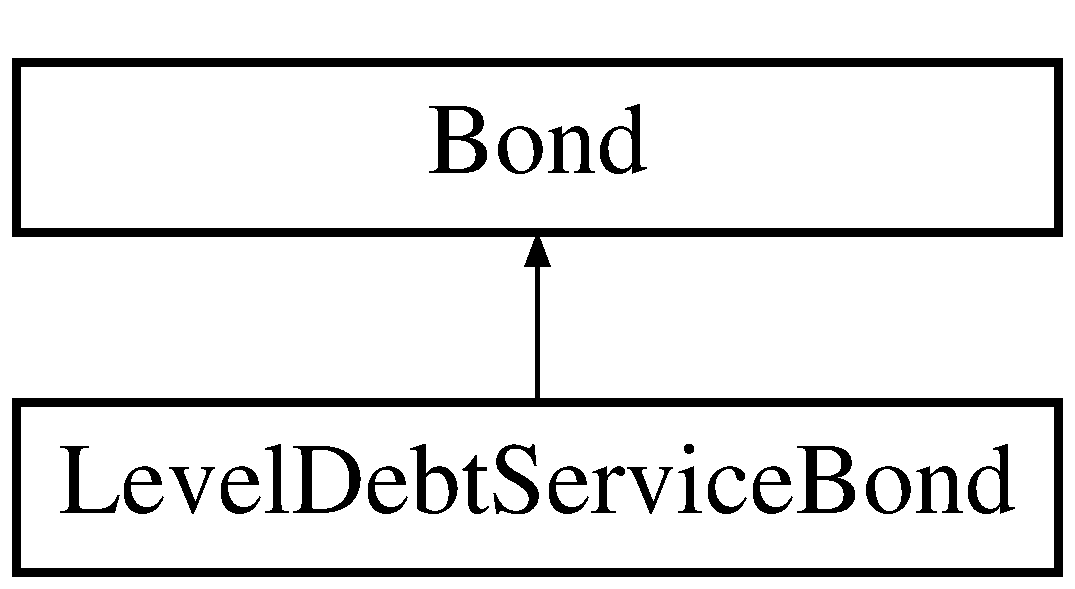
\includegraphics[height=2.000000cm]{classLevelDebtServiceBond}
\end{center}
\end{figure}
\subsection*{Public Member Functions}
\begin{DoxyCompactItemize}
\item 
\mbox{\hyperlink{classLevelDebtServiceBond_a71af87d057090bd2310a10df03b36fdf_a71af87d057090bd2310a10df03b36fdf}{Level\+Debt\+Service\+Bond}} (const int \mbox{\hyperlink{classBond_a7f75bcafbc16676ad6dbafbf40afae4a_a7f75bcafbc16676ad6dbafbf40afae4a}{id}}, const double \mbox{\hyperlink{classBond_ad98df7d28b398e620286f95ee085439b_ad98df7d28b398e620286f95ee085439b}{cost\+\_\+of\+\_\+capital}}, const int \mbox{\hyperlink{classBond_a4a227b6de2eeada118d82ab1633b1db8_a4a227b6de2eeada118d82ab1633b1db8}{n\+\_\+payments}}, const double \mbox{\hyperlink{classBond_a5f66785534e24caa43d9f730130a6463_a5f66785534e24caa43d9f730130a6463}{coupon\+\_\+rate}}, vector$<$ int $>$ \mbox{\hyperlink{classBond_ae8dd46fcbf95c993460ffe4ea1f52739_ae8dd46fcbf95c993460ffe4ea1f52739}{pay\+\_\+on\+\_\+weeks}}, bool begin\+\_\+repayment\+\_\+at\+\_\+issuance=false)
\item 
\mbox{\hyperlink{classLevelDebtServiceBond_a6327829c1f1e6941cc22cea371cf024a_a6327829c1f1e6941cc22cea371cf024a}{$\sim$\+Level\+Debt\+Service\+Bond}} () override
\item 
double \mbox{\hyperlink{classLevelDebtServiceBond_adcb3bd3c34b0cbb7b013f387ddd8b7f5_adcb3bd3c34b0cbb7b013f387ddd8b7f5}{get\+Debt\+Service}} (int week) override
\item 
double \mbox{\hyperlink{classLevelDebtServiceBond_a0f5820c3e76b8b908dbe153a8291d96a_a0f5820c3e76b8b908dbe153a8291d96a}{get\+Net\+Present\+Value\+At\+Issuance}} (double yearly\+\_\+discount\+\_\+rate, int week) const override
\item 
void \mbox{\hyperlink{classLevelDebtServiceBond_a51a54a1a25be105b168bf86489aee417_a51a54a1a25be105b168bf86489aee417}{issue\+Bond}} (int week, int construction\+\_\+time, double bond\+\_\+term\+\_\+multiplier, double bond\+\_\+interest\+\_\+rate\+\_\+multiplier) override
\end{DoxyCompactItemize}
\subsection*{Private Attributes}
\begin{DoxyCompactItemize}
\item 
double \mbox{\hyperlink{classLevelDebtServiceBond_a2af3b9ff7546bd002f78d07dbf696c64_a2af3b9ff7546bd002f78d07dbf696c64}{level\+\_\+debt\+\_\+service\+\_\+payment}}
\item 
int \mbox{\hyperlink{classLevelDebtServiceBond_ad1b8ba91ef3702a5eecfe3075fed0bc3_ad1b8ba91ef3702a5eecfe3075fed0bc3}{n\+\_\+payments\+\_\+made}} = 0
\end{DoxyCompactItemize}
\subsection*{Additional Inherited Members}


\subsection{Constructor \& Destructor Documentation}
\mbox{\Hypertarget{classLevelDebtServiceBond_a71af87d057090bd2310a10df03b36fdf_a71af87d057090bd2310a10df03b36fdf}\label{classLevelDebtServiceBond_a71af87d057090bd2310a10df03b36fdf_a71af87d057090bd2310a10df03b36fdf}} 
\index{Level\+Debt\+Service\+Bond@{Level\+Debt\+Service\+Bond}!Level\+Debt\+Service\+Bond@{Level\+Debt\+Service\+Bond}}
\index{Level\+Debt\+Service\+Bond@{Level\+Debt\+Service\+Bond}!Level\+Debt\+Service\+Bond@{Level\+Debt\+Service\+Bond}}
\subsubsection{\texorpdfstring{Level\+Debt\+Service\+Bond()}{LevelDebtServiceBond()}}
{\footnotesize\ttfamily Level\+Debt\+Service\+Bond\+::\+Level\+Debt\+Service\+Bond (\begin{DoxyParamCaption}\item[{const int}]{id,  }\item[{const double}]{cost\+\_\+of\+\_\+capital,  }\item[{const int}]{n\+\_\+payments,  }\item[{const double}]{coupon\+\_\+rate,  }\item[{vector$<$ int $>$}]{pay\+\_\+on\+\_\+weeks,  }\item[{bool}]{begin\+\_\+repayment\+\_\+at\+\_\+issuance = {\ttfamily false} }\end{DoxyParamCaption})}

\mbox{\Hypertarget{classLevelDebtServiceBond_a6327829c1f1e6941cc22cea371cf024a_a6327829c1f1e6941cc22cea371cf024a}\label{classLevelDebtServiceBond_a6327829c1f1e6941cc22cea371cf024a_a6327829c1f1e6941cc22cea371cf024a}} 
\index{Level\+Debt\+Service\+Bond@{Level\+Debt\+Service\+Bond}!````~Level\+Debt\+Service\+Bond@{$\sim$\+Level\+Debt\+Service\+Bond}}
\index{````~Level\+Debt\+Service\+Bond@{$\sim$\+Level\+Debt\+Service\+Bond}!Level\+Debt\+Service\+Bond@{Level\+Debt\+Service\+Bond}}
\subsubsection{\texorpdfstring{$\sim$\+Level\+Debt\+Service\+Bond()}{~LevelDebtServiceBond()}}
{\footnotesize\ttfamily Level\+Debt\+Service\+Bond\+::$\sim$\+Level\+Debt\+Service\+Bond (\begin{DoxyParamCaption}{ }\end{DoxyParamCaption})\hspace{0.3cm}{\ttfamily [override]}, {\ttfamily [default]}}



\subsection{Member Function Documentation}
\mbox{\Hypertarget{classLevelDebtServiceBond_adcb3bd3c34b0cbb7b013f387ddd8b7f5_adcb3bd3c34b0cbb7b013f387ddd8b7f5}\label{classLevelDebtServiceBond_adcb3bd3c34b0cbb7b013f387ddd8b7f5_adcb3bd3c34b0cbb7b013f387ddd8b7f5}} 
\index{Level\+Debt\+Service\+Bond@{Level\+Debt\+Service\+Bond}!get\+Debt\+Service@{get\+Debt\+Service}}
\index{get\+Debt\+Service@{get\+Debt\+Service}!Level\+Debt\+Service\+Bond@{Level\+Debt\+Service\+Bond}}
\subsubsection{\texorpdfstring{get\+Debt\+Service()}{getDebtService()}}
{\footnotesize\ttfamily double Level\+Debt\+Service\+Bond\+::get\+Debt\+Service (\begin{DoxyParamCaption}\item[{int}]{week }\end{DoxyParamCaption})\hspace{0.3cm}{\ttfamily [override]}, {\ttfamily [virtual]}}

Calculates debt service payment for a give week. 
\begin{DoxyParams}{Parameters}
{\em week} & \\
\hline
\end{DoxyParams}
\begin{DoxyReturn}{Returns}

\end{DoxyReturn}
If there are still payments to be made, repayment has begun, and this is a payment week, issue payment. 

Implements \mbox{\hyperlink{classBond_a98d8ecaf4b36319674ebd220598996bc_a98d8ecaf4b36319674ebd220598996bc}{Bond}}.

\mbox{\Hypertarget{classLevelDebtServiceBond_a0f5820c3e76b8b908dbe153a8291d96a_a0f5820c3e76b8b908dbe153a8291d96a}\label{classLevelDebtServiceBond_a0f5820c3e76b8b908dbe153a8291d96a_a0f5820c3e76b8b908dbe153a8291d96a}} 
\index{Level\+Debt\+Service\+Bond@{Level\+Debt\+Service\+Bond}!get\+Net\+Present\+Value\+At\+Issuance@{get\+Net\+Present\+Value\+At\+Issuance}}
\index{get\+Net\+Present\+Value\+At\+Issuance@{get\+Net\+Present\+Value\+At\+Issuance}!Level\+Debt\+Service\+Bond@{Level\+Debt\+Service\+Bond}}
\subsubsection{\texorpdfstring{get\+Net\+Present\+Value\+At\+Issuance()}{getNetPresentValueAtIssuance()}}
{\footnotesize\ttfamily double Level\+Debt\+Service\+Bond\+::get\+Net\+Present\+Value\+At\+Issuance (\begin{DoxyParamCaption}\item[{double}]{yearly\+\_\+discount\+\_\+rate,  }\item[{int}]{week }\end{DoxyParamCaption}) const\hspace{0.3cm}{\ttfamily [override]}, {\ttfamily [virtual]}}



Implements \mbox{\hyperlink{classBond_a5997278813deb16aa5d01bbca8ecc7b2_a5997278813deb16aa5d01bbca8ecc7b2}{Bond}}.

\mbox{\Hypertarget{classLevelDebtServiceBond_a51a54a1a25be105b168bf86489aee417_a51a54a1a25be105b168bf86489aee417}\label{classLevelDebtServiceBond_a51a54a1a25be105b168bf86489aee417_a51a54a1a25be105b168bf86489aee417}} 
\index{Level\+Debt\+Service\+Bond@{Level\+Debt\+Service\+Bond}!issue\+Bond@{issue\+Bond}}
\index{issue\+Bond@{issue\+Bond}!Level\+Debt\+Service\+Bond@{Level\+Debt\+Service\+Bond}}
\subsubsection{\texorpdfstring{issue\+Bond()}{issueBond()}}
{\footnotesize\ttfamily void Level\+Debt\+Service\+Bond\+::issue\+Bond (\begin{DoxyParamCaption}\item[{int}]{week,  }\item[{int}]{construction\+\_\+time,  }\item[{double}]{bond\+\_\+term\+\_\+multiplier,  }\item[{double}]{bond\+\_\+interest\+\_\+rate\+\_\+multiplier }\end{DoxyParamCaption})\hspace{0.3cm}{\ttfamily [override]}, {\ttfamily [virtual]}}

Level debt service payment value 

Reimplemented from \mbox{\hyperlink{classBond_a377db8c18b83c4666e46686bc26adef1_a377db8c18b83c4666e46686bc26adef1}{Bond}}.



\subsection{Field Documentation}
\mbox{\Hypertarget{classLevelDebtServiceBond_a2af3b9ff7546bd002f78d07dbf696c64_a2af3b9ff7546bd002f78d07dbf696c64}\label{classLevelDebtServiceBond_a2af3b9ff7546bd002f78d07dbf696c64_a2af3b9ff7546bd002f78d07dbf696c64}} 
\index{Level\+Debt\+Service\+Bond@{Level\+Debt\+Service\+Bond}!level\+\_\+debt\+\_\+service\+\_\+payment@{level\+\_\+debt\+\_\+service\+\_\+payment}}
\index{level\+\_\+debt\+\_\+service\+\_\+payment@{level\+\_\+debt\+\_\+service\+\_\+payment}!Level\+Debt\+Service\+Bond@{Level\+Debt\+Service\+Bond}}
\subsubsection{\texorpdfstring{level\+\_\+debt\+\_\+service\+\_\+payment}{level\_debt\_service\_payment}}
{\footnotesize\ttfamily double Level\+Debt\+Service\+Bond\+::level\+\_\+debt\+\_\+service\+\_\+payment\hspace{0.3cm}{\ttfamily [private]}}

\mbox{\Hypertarget{classLevelDebtServiceBond_ad1b8ba91ef3702a5eecfe3075fed0bc3_ad1b8ba91ef3702a5eecfe3075fed0bc3}\label{classLevelDebtServiceBond_ad1b8ba91ef3702a5eecfe3075fed0bc3_ad1b8ba91ef3702a5eecfe3075fed0bc3}} 
\index{Level\+Debt\+Service\+Bond@{Level\+Debt\+Service\+Bond}!n\+\_\+payments\+\_\+made@{n\+\_\+payments\+\_\+made}}
\index{n\+\_\+payments\+\_\+made@{n\+\_\+payments\+\_\+made}!Level\+Debt\+Service\+Bond@{Level\+Debt\+Service\+Bond}}
\subsubsection{\texorpdfstring{n\+\_\+payments\+\_\+made}{n\_payments\_made}}
{\footnotesize\ttfamily int Level\+Debt\+Service\+Bond\+::n\+\_\+payments\+\_\+made = 0\hspace{0.3cm}{\ttfamily [private]}}



The documentation for this class was generated from the following files\+:\begin{DoxyCompactItemize}
\item 
src/\+System\+Components/\+Bonds/\mbox{\hyperlink{LevelDebtServiceBond_8h}{Level\+Debt\+Service\+Bond.\+h}}\item 
src/\+System\+Components/\+Bonds/\mbox{\hyperlink{LevelDebtServiceBond_8cpp}{Level\+Debt\+Service\+Bond.\+cpp}}\end{DoxyCompactItemize}

\hypertarget{classPaperTestProblem}{}\section{Paper\+Test\+Problem Class Reference}
\label{classPaperTestProblem}\index{Paper\+Test\+Problem@{Paper\+Test\+Problem}}


{\ttfamily \#include $<$Paper\+Test\+Problem.\+h$>$}

Inheritance diagram for Paper\+Test\+Problem\+:\begin{figure}[H]
\begin{center}
\leavevmode
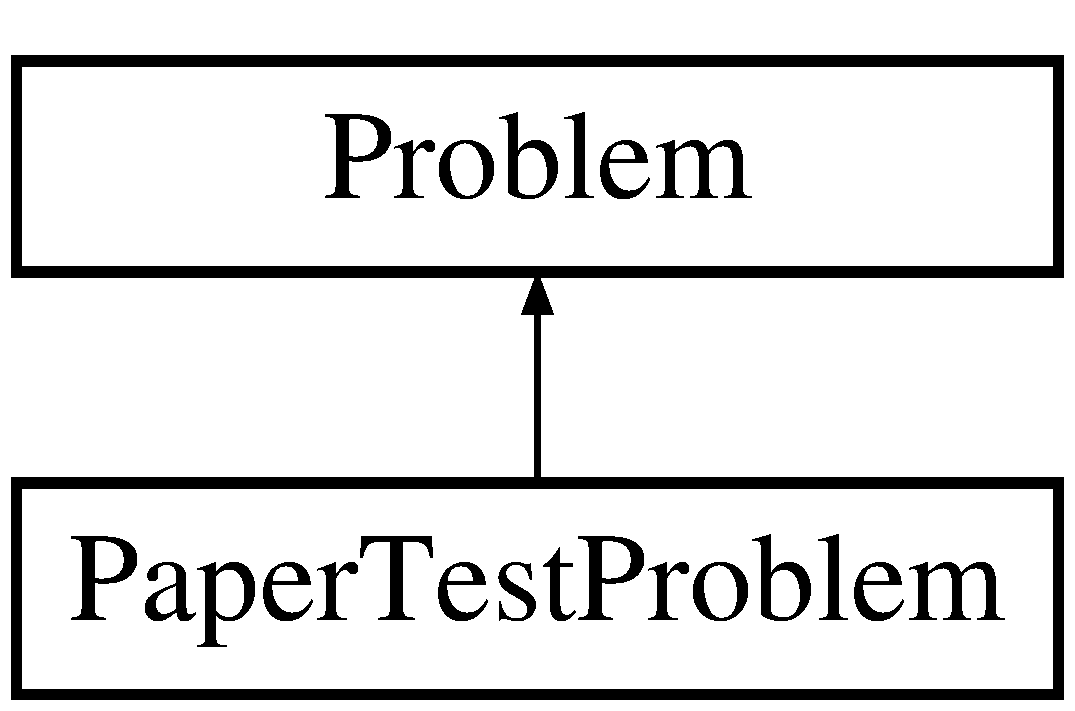
\includegraphics[height=2.000000cm]{classPaperTestProblem}
\end{center}
\end{figure}
\subsection*{Public Member Functions}
\begin{DoxyCompactItemize}
\item 
\mbox{\hyperlink{classPaperTestProblem_acc053a5b4515f3959494ce58c763d582}{Paper\+Test\+Problem}} (unsigned long \mbox{\hyperlink{classProblem_ac7513bb0ecdfa4bbb7d2ada3595d71ec}{n\+\_\+weeks}}, int import\+\_\+export\+\_\+rof\+\_\+table)
\item 
\mbox{\hyperlink{classPaperTestProblem_a571a92266d4c58ebc27e20391f7ad81b}{$\sim$\+Paper\+Test\+Problem}} () override
\item 
int \mbox{\hyperlink{classPaperTestProblem_a6db78df74d40f69a750b164caaca75c7}{function\+Evaluation}} (double $\ast$vars, double $\ast$objs, double $\ast$consts) override
\item 
void \mbox{\hyperlink{classPaperTestProblem_ae4bcc17d6ceab628f88174306d54fdc9}{read\+Input\+Data}} ()
\end{DoxyCompactItemize}
\subsection*{Additional Inherited Members}


\subsection{Constructor \& Destructor Documentation}
\mbox{\Hypertarget{classPaperTestProblem_acc053a5b4515f3959494ce58c763d582}\label{classPaperTestProblem_acc053a5b4515f3959494ce58c763d582}} 
\index{Paper\+Test\+Problem@{Paper\+Test\+Problem}!Paper\+Test\+Problem@{Paper\+Test\+Problem}}
\index{Paper\+Test\+Problem@{Paper\+Test\+Problem}!Paper\+Test\+Problem@{Paper\+Test\+Problem}}
\subsubsection{\texorpdfstring{Paper\+Test\+Problem()}{PaperTestProblem()}}
{\footnotesize\ttfamily Paper\+Test\+Problem\+::\+Paper\+Test\+Problem (\begin{DoxyParamCaption}\item[{unsigned long}]{n\+\_\+weeks,  }\item[{int}]{import\+\_\+export\+\_\+rof\+\_\+table }\end{DoxyParamCaption})}

\mbox{\Hypertarget{classPaperTestProblem_a571a92266d4c58ebc27e20391f7ad81b}\label{classPaperTestProblem_a571a92266d4c58ebc27e20391f7ad81b}} 
\index{Paper\+Test\+Problem@{Paper\+Test\+Problem}!````~Paper\+Test\+Problem@{$\sim$\+Paper\+Test\+Problem}}
\index{````~Paper\+Test\+Problem@{$\sim$\+Paper\+Test\+Problem}!Paper\+Test\+Problem@{Paper\+Test\+Problem}}
\subsubsection{\texorpdfstring{$\sim$\+Paper\+Test\+Problem()}{~PaperTestProblem()}}
{\footnotesize\ttfamily Paper\+Test\+Problem\+::$\sim$\+Paper\+Test\+Problem (\begin{DoxyParamCaption}{ }\end{DoxyParamCaption})\hspace{0.3cm}{\ttfamily [override]}}



\subsection{Member Function Documentation}
\mbox{\Hypertarget{classPaperTestProblem_a6db78df74d40f69a750b164caaca75c7}\label{classPaperTestProblem_a6db78df74d40f69a750b164caaca75c7}} 
\index{Paper\+Test\+Problem@{Paper\+Test\+Problem}!function\+Evaluation@{function\+Evaluation}}
\index{function\+Evaluation@{function\+Evaluation}!Paper\+Test\+Problem@{Paper\+Test\+Problem}}
\subsubsection{\texorpdfstring{function\+Evaluation()}{functionEvaluation()}}
{\footnotesize\ttfamily int Paper\+Test\+Problem\+::function\+Evaluation (\begin{DoxyParamCaption}\item[{double $\ast$}]{vars,  }\item[{double $\ast$}]{objs,  }\item[{double $\ast$}]{consts }\end{DoxyParamCaption})\hspace{0.3cm}{\ttfamily [override]}, {\ttfamily [virtual]}}



Implements \mbox{\hyperlink{classProblem_acd924a80df4422c5199748c714e9405c}{Problem}}.

\mbox{\Hypertarget{classPaperTestProblem_ae4bcc17d6ceab628f88174306d54fdc9}\label{classPaperTestProblem_ae4bcc17d6ceab628f88174306d54fdc9}} 
\index{Paper\+Test\+Problem@{Paper\+Test\+Problem}!read\+Input\+Data@{read\+Input\+Data}}
\index{read\+Input\+Data@{read\+Input\+Data}!Paper\+Test\+Problem@{Paper\+Test\+Problem}}
\subsubsection{\texorpdfstring{read\+Input\+Data()}{readInputData()}}
{\footnotesize\ttfamily void Paper\+Test\+Problem\+::read\+Input\+Data (\begin{DoxyParamCaption}{ }\end{DoxyParamCaption})}



The documentation for this class was generated from the following file\+:\begin{DoxyCompactItemize}
\item 
/home/fs02/pmr82\+\_\+0001/lbl59/\+Water\+Paths-\/doc/src/\+Problem/\mbox{\hyperlink{PaperTestProblem_8h}{Paper\+Test\+Problem.\+h}}\end{DoxyCompactItemize}

\hypertarget{classProblem}{}\section{Problem Class Reference}
\label{classProblem}\index{Problem@{Problem}}


{\ttfamily \#include $<$Problem.\+h$>$}

Inheritance diagram for Problem\+:\begin{figure}[H]
\begin{center}
\leavevmode
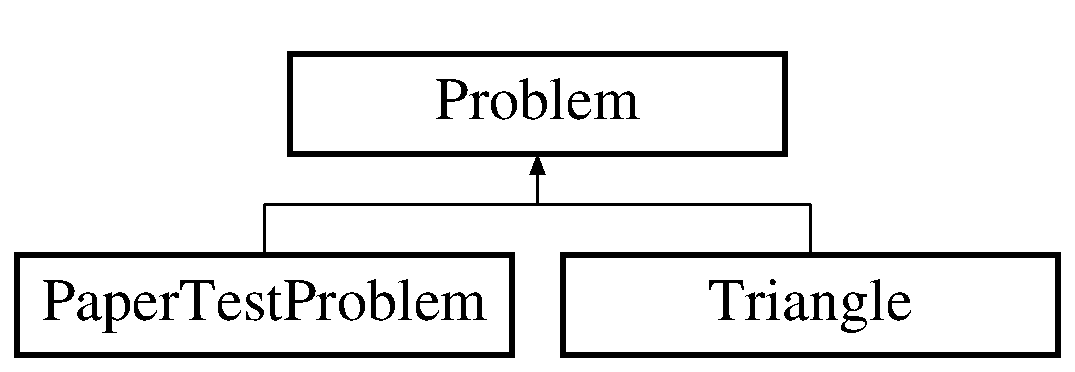
\includegraphics[height=2.000000cm]{classProblem}
\end{center}
\end{figure}
\subsection*{Public Member Functions}
\begin{DoxyCompactItemize}
\item 
\mbox{\hyperlink{classProblem_a41939e01b382197124fcd9f5e8c7520d}{Problem}} (unsigned long \mbox{\hyperlink{classProblem_ac7513bb0ecdfa4bbb7d2ada3595d71ec}{n\+\_\+weeks}})
\item 
virtual \mbox{\hyperlink{classProblem_a839a525ed01c34d57fff42583003d3e7}{$\sim$\+Problem}} ()
\item 
virtual int \mbox{\hyperlink{classProblem_acd924a80df4422c5199748c714e9405c}{function\+Evaluation}} (double $\ast$vars, double $\ast$objs, double $\ast$consts)=0
\item 
void \mbox{\hyperlink{classProblem_a1ea4a3d52209fa3f284a4060fb6fa3ab}{set\+N\+\_\+weeks}} (unsigned long \mbox{\hyperlink{classProblem_ac7513bb0ecdfa4bbb7d2ada3595d71ec}{n\+\_\+weeks}})
\item 
void \mbox{\hyperlink{classProblem_a855eaf9a98eadfab131d598b51df6d66}{set\+Sol\+\_\+number}} (unsigned long sol\+\_\+number)
\item 
void \mbox{\hyperlink{classProblem_a188254a95b04bf4ed67e66262ea342e9}{set\+I\+O\+Directory}} (const string \&\mbox{\hyperlink{classProblem_ac58848a0d808cf040c3fb3676b4a236f}{io\+\_\+directory}})
\item 
const vector$<$ double $>$ \& \mbox{\hyperlink{classProblem_a55da26d3bd669809b992fff823b8ef9b}{get\+Objectives}} () const
\item 
vector$<$ double $>$ \mbox{\hyperlink{classProblem_afdbe1eb541cc11071478da57b35e21b0}{calculate\+And\+Print\+Objectives}} (bool print\+\_\+files)
\item 
void \mbox{\hyperlink{classProblem_a98115002e741e9220f7aa6bae0cb179c}{set\+R\+D\+M\+Optimization}} (vector$<$ vector$<$ double $>$$>$ \&\mbox{\hyperlink{classProblem_aa4f6db22580c8d8a941e83556f4f5208}{utilities\+\_\+rdm}}, vector$<$ vector$<$ double $>$$>$ \&\mbox{\hyperlink{classProblem_ace43e5306285f0d91a199a4bd5a38922}{water\+\_\+sources\+\_\+rdm}}, vector$<$ vector$<$ double $>$$>$ \&\mbox{\hyperlink{classProblem_a63d49161a5d6d98e26cd218d90a13bae}{policies\+\_\+rdm}})
\item 
void \mbox{\hyperlink{classProblem_abaf4b2698552702ccf709bf07ed76ca3}{set\+R\+D\+M\+Reevaluation}} (unsigned long \mbox{\hyperlink{classProblem_a9e780729b6be5229c5bfa1e38c99cfa5}{rdm\+\_\+no}}, vector$<$ vector$<$ double $>$$>$ \&\mbox{\hyperlink{classProblem_aa4f6db22580c8d8a941e83556f4f5208}{utilities\+\_\+rdm}}, vector$<$ vector$<$ double $>$$>$ \&\mbox{\hyperlink{classProblem_ace43e5306285f0d91a199a4bd5a38922}{water\+\_\+sources\+\_\+rdm}}, vector$<$ vector$<$ double $>$$>$ \&\mbox{\hyperlink{classProblem_a63d49161a5d6d98e26cd218d90a13bae}{policies\+\_\+rdm}})
\item 
void \mbox{\hyperlink{classProblem_ad770920d19d5276fd0e30b835abe21ef}{set\+N\+\_\+threads}} (unsigned long \mbox{\hyperlink{classProblem_a3303a162d648e8ae16153b57b5b4054f}{n\+\_\+threads}})
\item 
void \mbox{\hyperlink{classProblem_a1f055d5e57392700cab27efdd4577be9}{set\+Print\+\_\+output\+\_\+files}} (bool \mbox{\hyperlink{classProblem_a3372a73270ce989f5d2056cace66215b}{print\+\_\+output\+\_\+files}})
\item 
void \mbox{\hyperlink{classProblem_ae5cec2ad575abb95cf7304153c31e410}{set\+N\+\_\+realizations}} (unsigned long \mbox{\hyperlink{classProblem_a270a5672643bfe09e52e0f24e1884136}{n\+\_\+realizations}})
\item 
void \mbox{\hyperlink{classProblem_afe5ddeb70b303e4971251e92a10f4828}{set\+Realizations\+To\+Run}} (vector$<$ unsigned long $>$ \&\mbox{\hyperlink{classProblem_af9ed9265d0d2b4918bd468d717429de1}{realizations\+\_\+to\+\_\+run}})
\item 
void \mbox{\hyperlink{classProblem_afb5e51664d0f340c393f7583622e99ca}{set\+Evap\+\_\+inflows\+\_\+suffix}} (const string \&\mbox{\hyperlink{classProblem_a1ff3958eef8bfb851a84ce0772104dca}{evap\+\_\+inflows\+\_\+suffix}})
\item 
void \mbox{\hyperlink{classProblem_ad666ae2c231f49103593a7e03a3b58fd}{set\+Fname\+\_\+sufix}} (const string \&\mbox{\hyperlink{classProblem_a59444139a907aaf4c6159caed46c8118}{fname\+\_\+sufix}})
\item 
\mbox{\hyperlink{classMasterDataCollector}{Master\+Data\+Collector}} $\ast$ \mbox{\hyperlink{classProblem_afce904c6b3bc58d029da4d9077efe4c9}{get\+Master\+\_\+data\+\_\+collector}} ()
\item 
void \mbox{\hyperlink{classProblem_af87d1081eb2a8fa57fa7f2666292fee3}{destroy\+Data\+Collector}} ()
\item 
void \mbox{\hyperlink{classProblem_a77568843acf22f2ecd17a83a1f3f310a}{print\+Time\+Series\+And\+Pathways}} ()
\item 
void \mbox{\hyperlink{classProblem_aa9debdf28260fd9054f7d6d2ee516f94}{set\+Rof\+Tables}} (unsigned long \mbox{\hyperlink{classProblem_a270a5672643bfe09e52e0f24e1884136}{n\+\_\+realizations}}, string \mbox{\hyperlink{classProblem_abc641b49a4defb0dbabafbf3f9dbca6e}{rof\+\_\+tables\+\_\+directory}})
\item 
void \mbox{\hyperlink{classProblem_a13b247f6699ebad04cbd5df07e681ba0}{set\+Import\+\_\+export\+\_\+rof\+\_\+tables}} (int \mbox{\hyperlink{classProblem_ac5a286f34cec786a0ad56c77783a201c}{import\+\_\+export\+\_\+rof\+\_\+tables}}, int \mbox{\hyperlink{classProblem_ac7513bb0ecdfa4bbb7d2ada3595d71ec}{n\+\_\+weeks}}, string \mbox{\hyperlink{classProblem_abc641b49a4defb0dbabafbf3f9dbca6e}{rof\+\_\+tables\+\_\+directory}})
\item 
void \mbox{\hyperlink{classProblem_a3604aafc0cf731fc9dfa8589ec8995ce}{run\+Bootstrap\+Realization\+Thinning}} (int standard\+\_\+solution, int n\+\_\+sets, int n\+\_\+bs\+\_\+samples, int threads, vector$<$ vector$<$ int $>$$>$ \&\mbox{\hyperlink{classProblem_af9ed9265d0d2b4918bd468d717429de1}{realizations\+\_\+to\+\_\+run}})
\end{DoxyCompactItemize}
\subsection*{Protected Member Functions}
\begin{DoxyCompactItemize}
\item 
double \mbox{\hyperlink{classProblem_ab9750751c2d4468a3dfe5dd6573b5179}{check\+And\+Fix\+Infra\+Expansion\+High\+Low\+Order}} (vector$<$ int $>$ $\ast$order, vector$<$ double $>$ $\ast$trigger, int id\+\_\+low, int id\+\_\+high, double capacity\+\_\+low, double capacity\+\_\+high)
\item 
vector$<$ int $>$ \mbox{\hyperlink{classProblem_ac157541eb885c80f2d2f23cc97a6a997}{vec\+Infra\+Rank\+To\+Vec\+Int}} (vector$<$ \mbox{\hyperlink{structinfraRank}{infra\+Rank}} $>$ v)
\end{DoxyCompactItemize}
\subsection*{Protected Attributes}
\begin{DoxyCompactItemize}
\item 
unsigned long \mbox{\hyperlink{classProblem_a270a5672643bfe09e52e0f24e1884136}{n\+\_\+realizations}}
\item 
unsigned long \mbox{\hyperlink{classProblem_ac7513bb0ecdfa4bbb7d2ada3595d71ec}{n\+\_\+weeks}}
\item 
unsigned long \mbox{\hyperlink{classProblem_a7ca15cdcbff926ddca25bdee5984ffe5}{solution\+\_\+no}}
\item 
unsigned long \mbox{\hyperlink{classProblem_a3303a162d648e8ae16153b57b5b4054f}{n\+\_\+threads}}
\item 
int \mbox{\hyperlink{classProblem_a4ca86ba2f568d232cf0421d39acff113}{n\+\_\+utilities}} = N\+O\+N\+\_\+\+I\+N\+I\+T\+I\+A\+L\+I\+Z\+ED
\item 
string \mbox{\hyperlink{classProblem_ac58848a0d808cf040c3fb3676b4a236f}{io\+\_\+directory}}
\item 
string \mbox{\hyperlink{classProblem_a59444139a907aaf4c6159caed46c8118}{fname\+\_\+sufix}}
\item 
string \mbox{\hyperlink{classProblem_a1ff3958eef8bfb851a84ce0772104dca}{evap\+\_\+inflows\+\_\+suffix}}
\item 
string \mbox{\hyperlink{classProblem_abc641b49a4defb0dbabafbf3f9dbca6e}{rof\+\_\+tables\+\_\+directory}}
\item 
vector$<$ unsigned long $>$ \mbox{\hyperlink{classProblem_af9ed9265d0d2b4918bd468d717429de1}{realizations\+\_\+to\+\_\+run}}
\item 
\mbox{\hyperlink{classMasterDataCollector}{Master\+Data\+Collector}} $\ast$ \mbox{\hyperlink{classProblem_a6cd1db1d587a449985d6514390ba8c96}{master\+\_\+data\+\_\+collector}} = nullptr
\item 
vector$<$ double $>$ \mbox{\hyperlink{classProblem_a72750ee8c8117f5ee9b190a359d6a60d}{objectives}}
\item 
bool \mbox{\hyperlink{classProblem_a3372a73270ce989f5d2056cace66215b}{print\+\_\+output\+\_\+files}} = true
\item 
unsigned long \mbox{\hyperlink{classProblem_a9e780729b6be5229c5bfa1e38c99cfa5}{rdm\+\_\+no}}
\item 
int \mbox{\hyperlink{classProblem_ac5a286f34cec786a0ad56c77783a201c}{import\+\_\+export\+\_\+rof\+\_\+tables}}
\item 
double \mbox{\hyperlink{classProblem_a27cae146b3409021f6d5936404cd1083}{table\+\_\+gen\+\_\+storage\+\_\+multiplier}}
\item 
vector$<$ vector$<$ double $>$ $>$ \mbox{\hyperlink{classProblem_aa4f6db22580c8d8a941e83556f4f5208}{utilities\+\_\+rdm}}
\item 
vector$<$ vector$<$ double $>$ $>$ \mbox{\hyperlink{classProblem_ace43e5306285f0d91a199a4bd5a38922}{water\+\_\+sources\+\_\+rdm}}
\item 
vector$<$ vector$<$ double $>$ $>$ \mbox{\hyperlink{classProblem_a63d49161a5d6d98e26cd218d90a13bae}{policies\+\_\+rdm}}
\item 
vector$<$ vector$<$ \mbox{\hyperlink{classMatrix2D}{Matrix2D}}$<$ double $>$ $>$ $>$ \mbox{\hyperlink{classProblem_a0a64a8c04964a326879eccccf5437c93}{rof\+\_\+tables}}
\end{DoxyCompactItemize}


\subsection{Constructor \& Destructor Documentation}
\mbox{\Hypertarget{classProblem_a41939e01b382197124fcd9f5e8c7520d}\label{classProblem_a41939e01b382197124fcd9f5e8c7520d}} 
\index{Problem@{Problem}!Problem@{Problem}}
\index{Problem@{Problem}!Problem@{Problem}}
\subsubsection{\texorpdfstring{Problem()}{Problem()}}
{\footnotesize\ttfamily Problem\+::\+Problem (\begin{DoxyParamCaption}\item[{unsigned long}]{n\+\_\+weeks }\end{DoxyParamCaption})}

\mbox{\Hypertarget{classProblem_a839a525ed01c34d57fff42583003d3e7}\label{classProblem_a839a525ed01c34d57fff42583003d3e7}} 
\index{Problem@{Problem}!````~Problem@{$\sim$\+Problem}}
\index{````~Problem@{$\sim$\+Problem}!Problem@{Problem}}
\subsubsection{\texorpdfstring{$\sim$\+Problem()}{~Problem()}}
{\footnotesize\ttfamily Problem\+::$\sim$\+Problem (\begin{DoxyParamCaption}{ }\end{DoxyParamCaption})\hspace{0.3cm}{\ttfamily [virtual]}}



\subsection{Member Function Documentation}
\mbox{\Hypertarget{classProblem_afdbe1eb541cc11071478da57b35e21b0}\label{classProblem_afdbe1eb541cc11071478da57b35e21b0}} 
\index{Problem@{Problem}!calculate\+And\+Print\+Objectives@{calculate\+And\+Print\+Objectives}}
\index{calculate\+And\+Print\+Objectives@{calculate\+And\+Print\+Objectives}!Problem@{Problem}}
\subsubsection{\texorpdfstring{calculate\+And\+Print\+Objectives()}{calculateAndPrintObjectives()}}
{\footnotesize\ttfamily vector$<$ double $>$ Problem\+::calculate\+And\+Print\+Objectives (\begin{DoxyParamCaption}\item[{bool}]{print\+\_\+files }\end{DoxyParamCaption})}

\mbox{\Hypertarget{classProblem_ab9750751c2d4468a3dfe5dd6573b5179}\label{classProblem_ab9750751c2d4468a3dfe5dd6573b5179}} 
\index{Problem@{Problem}!check\+And\+Fix\+Infra\+Expansion\+High\+Low\+Order@{check\+And\+Fix\+Infra\+Expansion\+High\+Low\+Order}}
\index{check\+And\+Fix\+Infra\+Expansion\+High\+Low\+Order@{check\+And\+Fix\+Infra\+Expansion\+High\+Low\+Order}!Problem@{Problem}}
\subsubsection{\texorpdfstring{check\+And\+Fix\+Infra\+Expansion\+High\+Low\+Order()}{checkAndFixInfraExpansionHighLowOrder()}}
{\footnotesize\ttfamily double Problem\+::check\+And\+Fix\+Infra\+Expansion\+High\+Low\+Order (\begin{DoxyParamCaption}\item[{vector$<$ int $>$ $\ast$}]{order,  }\item[{vector$<$ double $>$ $\ast$}]{trigger,  }\item[{int}]{id\+\_\+low,  }\item[{int}]{id\+\_\+high,  }\item[{double}]{capacity\+\_\+low,  }\item[{double}]{capacity\+\_\+high }\end{DoxyParamCaption})\hspace{0.3cm}{\ttfamily [protected]}}

\mbox{\Hypertarget{classProblem_af87d1081eb2a8fa57fa7f2666292fee3}\label{classProblem_af87d1081eb2a8fa57fa7f2666292fee3}} 
\index{Problem@{Problem}!destroy\+Data\+Collector@{destroy\+Data\+Collector}}
\index{destroy\+Data\+Collector@{destroy\+Data\+Collector}!Problem@{Problem}}
\subsubsection{\texorpdfstring{destroy\+Data\+Collector()}{destroyDataCollector()}}
{\footnotesize\ttfamily void Problem\+::destroy\+Data\+Collector (\begin{DoxyParamCaption}{ }\end{DoxyParamCaption})}

\mbox{\Hypertarget{classProblem_acd924a80df4422c5199748c714e9405c}\label{classProblem_acd924a80df4422c5199748c714e9405c}} 
\index{Problem@{Problem}!function\+Evaluation@{function\+Evaluation}}
\index{function\+Evaluation@{function\+Evaluation}!Problem@{Problem}}
\subsubsection{\texorpdfstring{function\+Evaluation()}{functionEvaluation()}}
{\footnotesize\ttfamily virtual int Problem\+::function\+Evaluation (\begin{DoxyParamCaption}\item[{double $\ast$}]{vars,  }\item[{double $\ast$}]{objs,  }\item[{double $\ast$}]{consts }\end{DoxyParamCaption})\hspace{0.3cm}{\ttfamily [pure virtual]}}



Implemented in \mbox{\hyperlink{classTriangle_a9e95039d098fd61cce1a830b85ed7004}{Triangle}}, and \mbox{\hyperlink{classPaperTestProblem_a6db78df74d40f69a750b164caaca75c7}{Paper\+Test\+Problem}}.

\mbox{\Hypertarget{classProblem_afce904c6b3bc58d029da4d9077efe4c9}\label{classProblem_afce904c6b3bc58d029da4d9077efe4c9}} 
\index{Problem@{Problem}!get\+Master\+\_\+data\+\_\+collector@{get\+Master\+\_\+data\+\_\+collector}}
\index{get\+Master\+\_\+data\+\_\+collector@{get\+Master\+\_\+data\+\_\+collector}!Problem@{Problem}}
\subsubsection{\texorpdfstring{get\+Master\+\_\+data\+\_\+collector()}{getMaster\_data\_collector()}}
{\footnotesize\ttfamily \mbox{\hyperlink{classMasterDataCollector}{Master\+Data\+Collector}} $\ast$ Problem\+::get\+Master\+\_\+data\+\_\+collector (\begin{DoxyParamCaption}{ }\end{DoxyParamCaption})}

\mbox{\Hypertarget{classProblem_a55da26d3bd669809b992fff823b8ef9b}\label{classProblem_a55da26d3bd669809b992fff823b8ef9b}} 
\index{Problem@{Problem}!get\+Objectives@{get\+Objectives}}
\index{get\+Objectives@{get\+Objectives}!Problem@{Problem}}
\subsubsection{\texorpdfstring{get\+Objectives()}{getObjectives()}}
{\footnotesize\ttfamily const vector$<$ double $>$ \& Problem\+::get\+Objectives (\begin{DoxyParamCaption}{ }\end{DoxyParamCaption}) const}

\mbox{\Hypertarget{classProblem_a77568843acf22f2ecd17a83a1f3f310a}\label{classProblem_a77568843acf22f2ecd17a83a1f3f310a}} 
\index{Problem@{Problem}!print\+Time\+Series\+And\+Pathways@{print\+Time\+Series\+And\+Pathways}}
\index{print\+Time\+Series\+And\+Pathways@{print\+Time\+Series\+And\+Pathways}!Problem@{Problem}}
\subsubsection{\texorpdfstring{print\+Time\+Series\+And\+Pathways()}{printTimeSeriesAndPathways()}}
{\footnotesize\ttfamily void Problem\+::print\+Time\+Series\+And\+Pathways (\begin{DoxyParamCaption}{ }\end{DoxyParamCaption})}

Calculate objective values.

Print output files. \mbox{\Hypertarget{classProblem_a3604aafc0cf731fc9dfa8589ec8995ce}\label{classProblem_a3604aafc0cf731fc9dfa8589ec8995ce}} 
\index{Problem@{Problem}!run\+Bootstrap\+Realization\+Thinning@{run\+Bootstrap\+Realization\+Thinning}}
\index{run\+Bootstrap\+Realization\+Thinning@{run\+Bootstrap\+Realization\+Thinning}!Problem@{Problem}}
\subsubsection{\texorpdfstring{run\+Bootstrap\+Realization\+Thinning()}{runBootstrapRealizationThinning()}}
{\footnotesize\ttfamily void Problem\+::run\+Bootstrap\+Realization\+Thinning (\begin{DoxyParamCaption}\item[{int}]{standard\+\_\+solution,  }\item[{int}]{n\+\_\+sets,  }\item[{int}]{n\+\_\+bs\+\_\+samples,  }\item[{int}]{threads,  }\item[{vector$<$ vector$<$ int $>$$>$ \&}]{realizations\+\_\+to\+\_\+run }\end{DoxyParamCaption})}

\mbox{\Hypertarget{classProblem_afb5e51664d0f340c393f7583622e99ca}\label{classProblem_afb5e51664d0f340c393f7583622e99ca}} 
\index{Problem@{Problem}!set\+Evap\+\_\+inflows\+\_\+suffix@{set\+Evap\+\_\+inflows\+\_\+suffix}}
\index{set\+Evap\+\_\+inflows\+\_\+suffix@{set\+Evap\+\_\+inflows\+\_\+suffix}!Problem@{Problem}}
\subsubsection{\texorpdfstring{set\+Evap\+\_\+inflows\+\_\+suffix()}{setEvap\_inflows\_suffix()}}
{\footnotesize\ttfamily void Problem\+::set\+Evap\+\_\+inflows\+\_\+suffix (\begin{DoxyParamCaption}\item[{const string \&}]{evap\+\_\+inflows\+\_\+suffix }\end{DoxyParamCaption})}

\mbox{\Hypertarget{classProblem_ad666ae2c231f49103593a7e03a3b58fd}\label{classProblem_ad666ae2c231f49103593a7e03a3b58fd}} 
\index{Problem@{Problem}!set\+Fname\+\_\+sufix@{set\+Fname\+\_\+sufix}}
\index{set\+Fname\+\_\+sufix@{set\+Fname\+\_\+sufix}!Problem@{Problem}}
\subsubsection{\texorpdfstring{set\+Fname\+\_\+sufix()}{setFname\_sufix()}}
{\footnotesize\ttfamily void Problem\+::set\+Fname\+\_\+sufix (\begin{DoxyParamCaption}\item[{const string \&}]{fname\+\_\+sufix }\end{DoxyParamCaption})}

\mbox{\Hypertarget{classProblem_a13b247f6699ebad04cbd5df07e681ba0}\label{classProblem_a13b247f6699ebad04cbd5df07e681ba0}} 
\index{Problem@{Problem}!set\+Import\+\_\+export\+\_\+rof\+\_\+tables@{set\+Import\+\_\+export\+\_\+rof\+\_\+tables}}
\index{set\+Import\+\_\+export\+\_\+rof\+\_\+tables@{set\+Import\+\_\+export\+\_\+rof\+\_\+tables}!Problem@{Problem}}
\subsubsection{\texorpdfstring{set\+Import\+\_\+export\+\_\+rof\+\_\+tables()}{setImport\_export\_rof\_tables()}}
{\footnotesize\ttfamily void Problem\+::set\+Import\+\_\+export\+\_\+rof\+\_\+tables (\begin{DoxyParamCaption}\item[{int}]{import\+\_\+export\+\_\+rof\+\_\+tables,  }\item[{int}]{n\+\_\+weeks,  }\item[{string}]{rof\+\_\+tables\+\_\+directory }\end{DoxyParamCaption})}

\mbox{\Hypertarget{classProblem_a188254a95b04bf4ed67e66262ea342e9}\label{classProblem_a188254a95b04bf4ed67e66262ea342e9}} 
\index{Problem@{Problem}!set\+I\+O\+Directory@{set\+I\+O\+Directory}}
\index{set\+I\+O\+Directory@{set\+I\+O\+Directory}!Problem@{Problem}}
\subsubsection{\texorpdfstring{set\+I\+O\+Directory()}{setIODirectory()}}
{\footnotesize\ttfamily void Problem\+::set\+I\+O\+Directory (\begin{DoxyParamCaption}\item[{const string \&}]{io\+\_\+directory }\end{DoxyParamCaption})}

\mbox{\Hypertarget{classProblem_ae5cec2ad575abb95cf7304153c31e410}\label{classProblem_ae5cec2ad575abb95cf7304153c31e410}} 
\index{Problem@{Problem}!set\+N\+\_\+realizations@{set\+N\+\_\+realizations}}
\index{set\+N\+\_\+realizations@{set\+N\+\_\+realizations}!Problem@{Problem}}
\subsubsection{\texorpdfstring{set\+N\+\_\+realizations()}{setN\_realizations()}}
{\footnotesize\ttfamily void Problem\+::set\+N\+\_\+realizations (\begin{DoxyParamCaption}\item[{unsigned long}]{n\+\_\+realizations }\end{DoxyParamCaption})}

\mbox{\Hypertarget{classProblem_ad770920d19d5276fd0e30b835abe21ef}\label{classProblem_ad770920d19d5276fd0e30b835abe21ef}} 
\index{Problem@{Problem}!set\+N\+\_\+threads@{set\+N\+\_\+threads}}
\index{set\+N\+\_\+threads@{set\+N\+\_\+threads}!Problem@{Problem}}
\subsubsection{\texorpdfstring{set\+N\+\_\+threads()}{setN\_threads()}}
{\footnotesize\ttfamily void Problem\+::set\+N\+\_\+threads (\begin{DoxyParamCaption}\item[{unsigned long}]{n\+\_\+threads }\end{DoxyParamCaption})}

\mbox{\Hypertarget{classProblem_a1ea4a3d52209fa3f284a4060fb6fa3ab}\label{classProblem_a1ea4a3d52209fa3f284a4060fb6fa3ab}} 
\index{Problem@{Problem}!set\+N\+\_\+weeks@{set\+N\+\_\+weeks}}
\index{set\+N\+\_\+weeks@{set\+N\+\_\+weeks}!Problem@{Problem}}
\subsubsection{\texorpdfstring{set\+N\+\_\+weeks()}{setN\_weeks()}}
{\footnotesize\ttfamily void Problem\+::set\+N\+\_\+weeks (\begin{DoxyParamCaption}\item[{unsigned long}]{n\+\_\+weeks }\end{DoxyParamCaption})}

\mbox{\Hypertarget{classProblem_a1f055d5e57392700cab27efdd4577be9}\label{classProblem_a1f055d5e57392700cab27efdd4577be9}} 
\index{Problem@{Problem}!set\+Print\+\_\+output\+\_\+files@{set\+Print\+\_\+output\+\_\+files}}
\index{set\+Print\+\_\+output\+\_\+files@{set\+Print\+\_\+output\+\_\+files}!Problem@{Problem}}
\subsubsection{\texorpdfstring{set\+Print\+\_\+output\+\_\+files()}{setPrint\_output\_files()}}
{\footnotesize\ttfamily void Problem\+::set\+Print\+\_\+output\+\_\+files (\begin{DoxyParamCaption}\item[{bool}]{print\+\_\+output\+\_\+files }\end{DoxyParamCaption})}

\mbox{\Hypertarget{classProblem_a98115002e741e9220f7aa6bae0cb179c}\label{classProblem_a98115002e741e9220f7aa6bae0cb179c}} 
\index{Problem@{Problem}!set\+R\+D\+M\+Optimization@{set\+R\+D\+M\+Optimization}}
\index{set\+R\+D\+M\+Optimization@{set\+R\+D\+M\+Optimization}!Problem@{Problem}}
\subsubsection{\texorpdfstring{set\+R\+D\+M\+Optimization()}{setRDMOptimization()}}
{\footnotesize\ttfamily void Problem\+::set\+R\+D\+M\+Optimization (\begin{DoxyParamCaption}\item[{vector$<$ vector$<$ double $>$$>$ \&}]{utilities\+\_\+rdm,  }\item[{vector$<$ vector$<$ double $>$$>$ \&}]{water\+\_\+sources\+\_\+rdm,  }\item[{vector$<$ vector$<$ double $>$$>$ \&}]{policies\+\_\+rdm }\end{DoxyParamCaption})}

\mbox{\Hypertarget{classProblem_abaf4b2698552702ccf709bf07ed76ca3}\label{classProblem_abaf4b2698552702ccf709bf07ed76ca3}} 
\index{Problem@{Problem}!set\+R\+D\+M\+Reevaluation@{set\+R\+D\+M\+Reevaluation}}
\index{set\+R\+D\+M\+Reevaluation@{set\+R\+D\+M\+Reevaluation}!Problem@{Problem}}
\subsubsection{\texorpdfstring{set\+R\+D\+M\+Reevaluation()}{setRDMReevaluation()}}
{\footnotesize\ttfamily void Problem\+::set\+R\+D\+M\+Reevaluation (\begin{DoxyParamCaption}\item[{unsigned long}]{rdm\+\_\+no,  }\item[{vector$<$ vector$<$ double $>$$>$ \&}]{utilities\+\_\+rdm,  }\item[{vector$<$ vector$<$ double $>$$>$ \&}]{water\+\_\+sources\+\_\+rdm,  }\item[{vector$<$ vector$<$ double $>$$>$ \&}]{policies\+\_\+rdm }\end{DoxyParamCaption})}

\mbox{\Hypertarget{classProblem_afe5ddeb70b303e4971251e92a10f4828}\label{classProblem_afe5ddeb70b303e4971251e92a10f4828}} 
\index{Problem@{Problem}!set\+Realizations\+To\+Run@{set\+Realizations\+To\+Run}}
\index{set\+Realizations\+To\+Run@{set\+Realizations\+To\+Run}!Problem@{Problem}}
\subsubsection{\texorpdfstring{set\+Realizations\+To\+Run()}{setRealizationsToRun()}}
{\footnotesize\ttfamily void Problem\+::set\+Realizations\+To\+Run (\begin{DoxyParamCaption}\item[{vector$<$ unsigned long $>$ \&}]{realizations\+\_\+to\+\_\+run }\end{DoxyParamCaption})}

\mbox{\Hypertarget{classProblem_aa9debdf28260fd9054f7d6d2ee516f94}\label{classProblem_aa9debdf28260fd9054f7d6d2ee516f94}} 
\index{Problem@{Problem}!set\+Rof\+Tables@{set\+Rof\+Tables}}
\index{set\+Rof\+Tables@{set\+Rof\+Tables}!Problem@{Problem}}
\subsubsection{\texorpdfstring{set\+Rof\+Tables()}{setRofTables()}}
{\footnotesize\ttfamily void Problem\+::set\+Rof\+Tables (\begin{DoxyParamCaption}\item[{unsigned long}]{n\+\_\+realizations,  }\item[{string}]{rof\+\_\+tables\+\_\+directory }\end{DoxyParamCaption})}

Read pre-\/computed R\+OF tables. 
\begin{DoxyParams}{Parameters}
{\em folder} & Folder containing the R\+OF tables. \\
\hline
{\em n\+\_\+realizations} & number of realizations. \\
\hline
\end{DoxyParams}
Get number of weeks in tables \mbox{\Hypertarget{classProblem_a855eaf9a98eadfab131d598b51df6d66}\label{classProblem_a855eaf9a98eadfab131d598b51df6d66}} 
\index{Problem@{Problem}!set\+Sol\+\_\+number@{set\+Sol\+\_\+number}}
\index{set\+Sol\+\_\+number@{set\+Sol\+\_\+number}!Problem@{Problem}}
\subsubsection{\texorpdfstring{set\+Sol\+\_\+number()}{setSol\_number()}}
{\footnotesize\ttfamily void Problem\+::set\+Sol\+\_\+number (\begin{DoxyParamCaption}\item[{unsigned long}]{sol\+\_\+number }\end{DoxyParamCaption})}

\mbox{\Hypertarget{classProblem_ac157541eb885c80f2d2f23cc97a6a997}\label{classProblem_ac157541eb885c80f2d2f23cc97a6a997}} 
\index{Problem@{Problem}!vec\+Infra\+Rank\+To\+Vec\+Int@{vec\+Infra\+Rank\+To\+Vec\+Int}}
\index{vec\+Infra\+Rank\+To\+Vec\+Int@{vec\+Infra\+Rank\+To\+Vec\+Int}!Problem@{Problem}}
\subsubsection{\texorpdfstring{vec\+Infra\+Rank\+To\+Vec\+Int()}{vecInfraRankToVecInt()}}
{\footnotesize\ttfamily vector$<$ int $>$ Problem\+::vec\+Infra\+Rank\+To\+Vec\+Int (\begin{DoxyParamCaption}\item[{vector$<$ \mbox{\hyperlink{structinfraRank}{infra\+Rank}} $>$}]{v }\end{DoxyParamCaption})\hspace{0.3cm}{\ttfamily [protected]}}



\subsection{Member Data Documentation}
\mbox{\Hypertarget{classProblem_a1ff3958eef8bfb851a84ce0772104dca}\label{classProblem_a1ff3958eef8bfb851a84ce0772104dca}} 
\index{Problem@{Problem}!evap\+\_\+inflows\+\_\+suffix@{evap\+\_\+inflows\+\_\+suffix}}
\index{evap\+\_\+inflows\+\_\+suffix@{evap\+\_\+inflows\+\_\+suffix}!Problem@{Problem}}
\subsubsection{\texorpdfstring{evap\+\_\+inflows\+\_\+suffix}{evap\_inflows\_suffix}}
{\footnotesize\ttfamily string Problem\+::evap\+\_\+inflows\+\_\+suffix\hspace{0.3cm}{\ttfamily [protected]}}

\mbox{\Hypertarget{classProblem_a59444139a907aaf4c6159caed46c8118}\label{classProblem_a59444139a907aaf4c6159caed46c8118}} 
\index{Problem@{Problem}!fname\+\_\+sufix@{fname\+\_\+sufix}}
\index{fname\+\_\+sufix@{fname\+\_\+sufix}!Problem@{Problem}}
\subsubsection{\texorpdfstring{fname\+\_\+sufix}{fname\_sufix}}
{\footnotesize\ttfamily string Problem\+::fname\+\_\+sufix\hspace{0.3cm}{\ttfamily [protected]}}

\mbox{\Hypertarget{classProblem_ac5a286f34cec786a0ad56c77783a201c}\label{classProblem_ac5a286f34cec786a0ad56c77783a201c}} 
\index{Problem@{Problem}!import\+\_\+export\+\_\+rof\+\_\+tables@{import\+\_\+export\+\_\+rof\+\_\+tables}}
\index{import\+\_\+export\+\_\+rof\+\_\+tables@{import\+\_\+export\+\_\+rof\+\_\+tables}!Problem@{Problem}}
\subsubsection{\texorpdfstring{import\+\_\+export\+\_\+rof\+\_\+tables}{import\_export\_rof\_tables}}
{\footnotesize\ttfamily int Problem\+::import\+\_\+export\+\_\+rof\+\_\+tables\hspace{0.3cm}{\ttfamily [protected]}}

\mbox{\Hypertarget{classProblem_ac58848a0d808cf040c3fb3676b4a236f}\label{classProblem_ac58848a0d808cf040c3fb3676b4a236f}} 
\index{Problem@{Problem}!io\+\_\+directory@{io\+\_\+directory}}
\index{io\+\_\+directory@{io\+\_\+directory}!Problem@{Problem}}
\subsubsection{\texorpdfstring{io\+\_\+directory}{io\_directory}}
{\footnotesize\ttfamily string Problem\+::io\+\_\+directory\hspace{0.3cm}{\ttfamily [protected]}}

\mbox{\Hypertarget{classProblem_a6cd1db1d587a449985d6514390ba8c96}\label{classProblem_a6cd1db1d587a449985d6514390ba8c96}} 
\index{Problem@{Problem}!master\+\_\+data\+\_\+collector@{master\+\_\+data\+\_\+collector}}
\index{master\+\_\+data\+\_\+collector@{master\+\_\+data\+\_\+collector}!Problem@{Problem}}
\subsubsection{\texorpdfstring{master\+\_\+data\+\_\+collector}{master\_data\_collector}}
{\footnotesize\ttfamily \mbox{\hyperlink{classMasterDataCollector}{Master\+Data\+Collector}}$\ast$ Problem\+::master\+\_\+data\+\_\+collector = nullptr\hspace{0.3cm}{\ttfamily [protected]}}

\mbox{\Hypertarget{classProblem_a270a5672643bfe09e52e0f24e1884136}\label{classProblem_a270a5672643bfe09e52e0f24e1884136}} 
\index{Problem@{Problem}!n\+\_\+realizations@{n\+\_\+realizations}}
\index{n\+\_\+realizations@{n\+\_\+realizations}!Problem@{Problem}}
\subsubsection{\texorpdfstring{n\+\_\+realizations}{n\_realizations}}
{\footnotesize\ttfamily unsigned long Problem\+::n\+\_\+realizations\hspace{0.3cm}{\ttfamily [protected]}}

\mbox{\Hypertarget{classProblem_a3303a162d648e8ae16153b57b5b4054f}\label{classProblem_a3303a162d648e8ae16153b57b5b4054f}} 
\index{Problem@{Problem}!n\+\_\+threads@{n\+\_\+threads}}
\index{n\+\_\+threads@{n\+\_\+threads}!Problem@{Problem}}
\subsubsection{\texorpdfstring{n\+\_\+threads}{n\_threads}}
{\footnotesize\ttfamily unsigned long Problem\+::n\+\_\+threads\hspace{0.3cm}{\ttfamily [protected]}}

\mbox{\Hypertarget{classProblem_a4ca86ba2f568d232cf0421d39acff113}\label{classProblem_a4ca86ba2f568d232cf0421d39acff113}} 
\index{Problem@{Problem}!n\+\_\+utilities@{n\+\_\+utilities}}
\index{n\+\_\+utilities@{n\+\_\+utilities}!Problem@{Problem}}
\subsubsection{\texorpdfstring{n\+\_\+utilities}{n\_utilities}}
{\footnotesize\ttfamily int Problem\+::n\+\_\+utilities = N\+O\+N\+\_\+\+I\+N\+I\+T\+I\+A\+L\+I\+Z\+ED\hspace{0.3cm}{\ttfamily [protected]}}

\mbox{\Hypertarget{classProblem_ac7513bb0ecdfa4bbb7d2ada3595d71ec}\label{classProblem_ac7513bb0ecdfa4bbb7d2ada3595d71ec}} 
\index{Problem@{Problem}!n\+\_\+weeks@{n\+\_\+weeks}}
\index{n\+\_\+weeks@{n\+\_\+weeks}!Problem@{Problem}}
\subsubsection{\texorpdfstring{n\+\_\+weeks}{n\_weeks}}
{\footnotesize\ttfamily unsigned long Problem\+::n\+\_\+weeks\hspace{0.3cm}{\ttfamily [protected]}}

\mbox{\Hypertarget{classProblem_a72750ee8c8117f5ee9b190a359d6a60d}\label{classProblem_a72750ee8c8117f5ee9b190a359d6a60d}} 
\index{Problem@{Problem}!objectives@{objectives}}
\index{objectives@{objectives}!Problem@{Problem}}
\subsubsection{\texorpdfstring{objectives}{objectives}}
{\footnotesize\ttfamily vector$<$double$>$ Problem\+::objectives\hspace{0.3cm}{\ttfamily [protected]}}

\mbox{\Hypertarget{classProblem_a63d49161a5d6d98e26cd218d90a13bae}\label{classProblem_a63d49161a5d6d98e26cd218d90a13bae}} 
\index{Problem@{Problem}!policies\+\_\+rdm@{policies\+\_\+rdm}}
\index{policies\+\_\+rdm@{policies\+\_\+rdm}!Problem@{Problem}}
\subsubsection{\texorpdfstring{policies\+\_\+rdm}{policies\_rdm}}
{\footnotesize\ttfamily vector$<$vector$<$double$>$ $>$ Problem\+::policies\+\_\+rdm\hspace{0.3cm}{\ttfamily [protected]}}

\mbox{\Hypertarget{classProblem_a3372a73270ce989f5d2056cace66215b}\label{classProblem_a3372a73270ce989f5d2056cace66215b}} 
\index{Problem@{Problem}!print\+\_\+output\+\_\+files@{print\+\_\+output\+\_\+files}}
\index{print\+\_\+output\+\_\+files@{print\+\_\+output\+\_\+files}!Problem@{Problem}}
\subsubsection{\texorpdfstring{print\+\_\+output\+\_\+files}{print\_output\_files}}
{\footnotesize\ttfamily bool Problem\+::print\+\_\+output\+\_\+files = true\hspace{0.3cm}{\ttfamily [protected]}}

\mbox{\Hypertarget{classProblem_a9e780729b6be5229c5bfa1e38c99cfa5}\label{classProblem_a9e780729b6be5229c5bfa1e38c99cfa5}} 
\index{Problem@{Problem}!rdm\+\_\+no@{rdm\+\_\+no}}
\index{rdm\+\_\+no@{rdm\+\_\+no}!Problem@{Problem}}
\subsubsection{\texorpdfstring{rdm\+\_\+no}{rdm\_no}}
{\footnotesize\ttfamily unsigned long Problem\+::rdm\+\_\+no\hspace{0.3cm}{\ttfamily [protected]}}

\mbox{\Hypertarget{classProblem_af9ed9265d0d2b4918bd468d717429de1}\label{classProblem_af9ed9265d0d2b4918bd468d717429de1}} 
\index{Problem@{Problem}!realizations\+\_\+to\+\_\+run@{realizations\+\_\+to\+\_\+run}}
\index{realizations\+\_\+to\+\_\+run@{realizations\+\_\+to\+\_\+run}!Problem@{Problem}}
\subsubsection{\texorpdfstring{realizations\+\_\+to\+\_\+run}{realizations\_to\_run}}
{\footnotesize\ttfamily vector$<$unsigned long $>$ Problem\+::realizations\+\_\+to\+\_\+run\hspace{0.3cm}{\ttfamily [protected]}}

\mbox{\Hypertarget{classProblem_a0a64a8c04964a326879eccccf5437c93}\label{classProblem_a0a64a8c04964a326879eccccf5437c93}} 
\index{Problem@{Problem}!rof\+\_\+tables@{rof\+\_\+tables}}
\index{rof\+\_\+tables@{rof\+\_\+tables}!Problem@{Problem}}
\subsubsection{\texorpdfstring{rof\+\_\+tables}{rof\_tables}}
{\footnotesize\ttfamily vector$<$vector$<$\mbox{\hyperlink{classMatrix2D}{Matrix2D}}$<$double$>$ $>$ $>$ Problem\+::rof\+\_\+tables\hspace{0.3cm}{\ttfamily [protected]}}

\mbox{\Hypertarget{classProblem_abc641b49a4defb0dbabafbf3f9dbca6e}\label{classProblem_abc641b49a4defb0dbabafbf3f9dbca6e}} 
\index{Problem@{Problem}!rof\+\_\+tables\+\_\+directory@{rof\+\_\+tables\+\_\+directory}}
\index{rof\+\_\+tables\+\_\+directory@{rof\+\_\+tables\+\_\+directory}!Problem@{Problem}}
\subsubsection{\texorpdfstring{rof\+\_\+tables\+\_\+directory}{rof\_tables\_directory}}
{\footnotesize\ttfamily string Problem\+::rof\+\_\+tables\+\_\+directory\hspace{0.3cm}{\ttfamily [protected]}}

\mbox{\Hypertarget{classProblem_a7ca15cdcbff926ddca25bdee5984ffe5}\label{classProblem_a7ca15cdcbff926ddca25bdee5984ffe5}} 
\index{Problem@{Problem}!solution\+\_\+no@{solution\+\_\+no}}
\index{solution\+\_\+no@{solution\+\_\+no}!Problem@{Problem}}
\subsubsection{\texorpdfstring{solution\+\_\+no}{solution\_no}}
{\footnotesize\ttfamily unsigned long Problem\+::solution\+\_\+no\hspace{0.3cm}{\ttfamily [protected]}}

\mbox{\Hypertarget{classProblem_a27cae146b3409021f6d5936404cd1083}\label{classProblem_a27cae146b3409021f6d5936404cd1083}} 
\index{Problem@{Problem}!table\+\_\+gen\+\_\+storage\+\_\+multiplier@{table\+\_\+gen\+\_\+storage\+\_\+multiplier}}
\index{table\+\_\+gen\+\_\+storage\+\_\+multiplier@{table\+\_\+gen\+\_\+storage\+\_\+multiplier}!Problem@{Problem}}
\subsubsection{\texorpdfstring{table\+\_\+gen\+\_\+storage\+\_\+multiplier}{table\_gen\_storage\_multiplier}}
{\footnotesize\ttfamily double Problem\+::table\+\_\+gen\+\_\+storage\+\_\+multiplier\hspace{0.3cm}{\ttfamily [protected]}}

\mbox{\Hypertarget{classProblem_aa4f6db22580c8d8a941e83556f4f5208}\label{classProblem_aa4f6db22580c8d8a941e83556f4f5208}} 
\index{Problem@{Problem}!utilities\+\_\+rdm@{utilities\+\_\+rdm}}
\index{utilities\+\_\+rdm@{utilities\+\_\+rdm}!Problem@{Problem}}
\subsubsection{\texorpdfstring{utilities\+\_\+rdm}{utilities\_rdm}}
{\footnotesize\ttfamily vector$<$vector$<$double$>$ $>$ Problem\+::utilities\+\_\+rdm\hspace{0.3cm}{\ttfamily [protected]}}

\mbox{\Hypertarget{classProblem_ace43e5306285f0d91a199a4bd5a38922}\label{classProblem_ace43e5306285f0d91a199a4bd5a38922}} 
\index{Problem@{Problem}!water\+\_\+sources\+\_\+rdm@{water\+\_\+sources\+\_\+rdm}}
\index{water\+\_\+sources\+\_\+rdm@{water\+\_\+sources\+\_\+rdm}!Problem@{Problem}}
\subsubsection{\texorpdfstring{water\+\_\+sources\+\_\+rdm}{water\_sources\_rdm}}
{\footnotesize\ttfamily vector$<$vector$<$double$>$ $>$ Problem\+::water\+\_\+sources\+\_\+rdm\hspace{0.3cm}{\ttfamily [protected]}}



The documentation for this class was generated from the following files\+:\begin{DoxyCompactItemize}
\item 
src/\+Problem/\+Base/\mbox{\hyperlink{Problem_8h}{Problem.\+h}}\item 
src/\+Problem/\+Base/\mbox{\hyperlink{Problem_8cpp}{Problem.\+cpp}}\end{DoxyCompactItemize}

\hypertarget{classQuarry}{}\section{Quarry Class Reference}
\label{classQuarry}\index{Quarry@{Quarry}}


{\ttfamily \#include $<$Quarry.\+h$>$}

Inheritance diagram for Quarry\+:\begin{figure}[H]
\begin{center}
\leavevmode
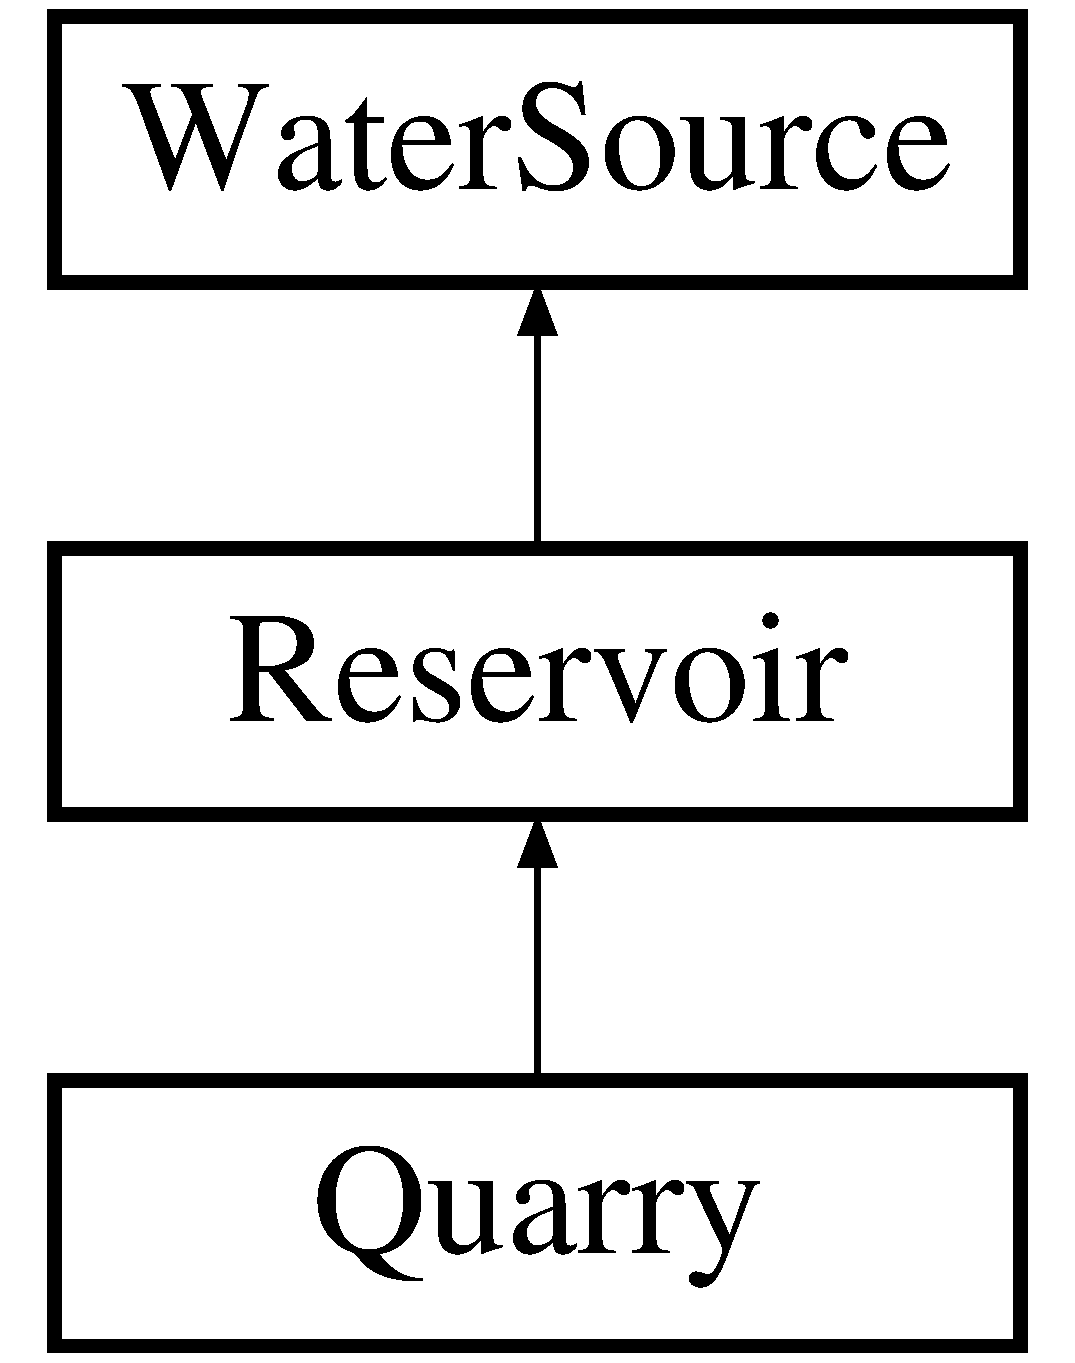
\includegraphics[height=3.000000cm]{classQuarry}
\end{center}
\end{figure}
\subsection*{Public Member Functions}
\begin{DoxyCompactItemize}
\item 
\mbox{\hyperlink{classQuarry_a126fddda9e5deeb667a6a9dbb0533470}{Quarry}} (const char $\ast$\mbox{\hyperlink{classWaterSource_a846ea74c5b453d014f594d41fee8c765}{name}}, const int \mbox{\hyperlink{classWaterSource_a6eafe5dfefd317877d1244e8a7c6e742}{id}}, const vector$<$ \mbox{\hyperlink{classCatchment}{Catchment}} $\ast$$>$ \&\mbox{\hyperlink{classWaterSource_a8c18c34f23f8a06685c1d12f462ed830}{catchments}}, const double \mbox{\hyperlink{classWaterSource_a2ec257b415b248214a8bce7fc5267723}{capacity}}, const double max\+\_\+treatment\+\_\+capacity, Evaporation\+Series \&\mbox{\hyperlink{classReservoir_a2d2d9b302c13703309bb798d24136810}{evaporation\+\_\+series}}, Data\+Series $\ast$\mbox{\hyperlink{classReservoir_a46bd5b750963dfa9a57b247fd77ab8ff}{storage\+\_\+area\+\_\+curve}}, double max\+\_\+diversion)
\begin{DoxyCompactList}\small\item\em Constructs a \mbox{\hyperlink{classQuarry}{Quarry}} object. This function initializes a quarry reservoir with specified parameters such as name, ID, catchments, capacity, treatment capacity, evaporation data, and more. \end{DoxyCompactList}\item 
\mbox{\hyperlink{classQuarry_a13cc1caeda6846900893f8d24c49b111}{Quarry}} (const char $\ast$\mbox{\hyperlink{classWaterSource_a846ea74c5b453d014f594d41fee8c765}{name}}, const int \mbox{\hyperlink{classWaterSource_a6eafe5dfefd317877d1244e8a7c6e742}{id}}, const vector$<$ \mbox{\hyperlink{classCatchment}{Catchment}} $\ast$$>$ \&\mbox{\hyperlink{classWaterSource_a8c18c34f23f8a06685c1d12f462ed830}{catchments}}, const double \mbox{\hyperlink{classWaterSource_a2ec257b415b248214a8bce7fc5267723}{capacity}}, const double max\+\_\+treatment\+\_\+capacity, Evaporation\+Series \&\mbox{\hyperlink{classReservoir_a2d2d9b302c13703309bb798d24136810}{evaporation\+\_\+series}}, Data\+Series $\ast$\mbox{\hyperlink{classReservoir_a46bd5b750963dfa9a57b247fd77ab8ff}{storage\+\_\+area\+\_\+curve}}, const vector$<$ double $>$ \&construction\+\_\+time\+\_\+range, double permitting\+\_\+period, \mbox{\hyperlink{classBond}{Bond}} \&bond, double max\+\_\+diversion)
\begin{DoxyCompactList}\small\item\em Constructs a \mbox{\hyperlink{classQuarry}{Quarry}} object. This function initializes a quarry reservoir with specified parameters such as name, ID, catchments, capacity, treatment capacity, evaporation data. It also includes additional parameters that define the construction timeline, and financial bond details. \end{DoxyCompactList}\item 
\mbox{\hyperlink{classQuarry_a28c4db26230c2ff3f82c8c0f70f2f124}{Quarry}} (const char $\ast$\mbox{\hyperlink{classWaterSource_a846ea74c5b453d014f594d41fee8c765}{name}}, const int \mbox{\hyperlink{classWaterSource_a6eafe5dfefd317877d1244e8a7c6e742}{id}}, const vector$<$ \mbox{\hyperlink{classCatchment}{Catchment}} $\ast$$>$ \&\mbox{\hyperlink{classWaterSource_a8c18c34f23f8a06685c1d12f462ed830}{catchments}}, const double \mbox{\hyperlink{classWaterSource_a2ec257b415b248214a8bce7fc5267723}{capacity}}, const double max\+\_\+treatment\+\_\+capacity, Evaporation\+Series \&\mbox{\hyperlink{classReservoir_a2d2d9b302c13703309bb798d24136810}{evaporation\+\_\+series}}, double storage\+\_\+area, double max\+\_\+diversion)
\begin{DoxyCompactList}\small\item\em Constructs a \mbox{\hyperlink{classQuarry}{Quarry}} object. This function initializes a quarry reservoir with specified parameters such as name, ID, catchments, capacity, treatment capacity, evaporation data. It specifies a fixed storage area instead of a storage area curve. \end{DoxyCompactList}\item 
\mbox{\hyperlink{classQuarry_a561616791620a55709bfca645bc8cbad}{Quarry}} (const char $\ast$\mbox{\hyperlink{classWaterSource_a846ea74c5b453d014f594d41fee8c765}{name}}, const int \mbox{\hyperlink{classWaterSource_a6eafe5dfefd317877d1244e8a7c6e742}{id}}, const vector$<$ \mbox{\hyperlink{classCatchment}{Catchment}} $\ast$$>$ \&\mbox{\hyperlink{classWaterSource_a8c18c34f23f8a06685c1d12f462ed830}{catchments}}, const double \mbox{\hyperlink{classWaterSource_a2ec257b415b248214a8bce7fc5267723}{capacity}}, const double max\+\_\+treatment\+\_\+capacity, Evaporation\+Series \&\mbox{\hyperlink{classReservoir_a2d2d9b302c13703309bb798d24136810}{evaporation\+\_\+series}}, double storage\+\_\+area, const vector$<$ double $>$ \&construction\+\_\+time\+\_\+range, double permitting\+\_\+period, \mbox{\hyperlink{classBond}{Bond}} \&bond, double max\+\_\+diversion)
\begin{DoxyCompactList}\small\item\em Constructs a \mbox{\hyperlink{classQuarry}{Quarry}} object. This function initializes a quarry reservoir with specified parameters such as name, ID, catchments, capacity, treatment capacity, evaporation data. It also includes additional parameters that define the construction timeline, and financial bond details. It specifies a fixed storage area instead of a storage area curve. \end{DoxyCompactList}\item 
\mbox{\hyperlink{classQuarry_a5a43f5a3f1cb837bc313046cf82b49e3}{Quarry}} (const \mbox{\hyperlink{classQuarry}{Quarry}} \&quarry, const double max\+\_\+diversion)
\begin{DoxyCompactList}\small\item\em Constructs a \mbox{\hyperlink{classQuarry}{Quarry}} object as a copy of an existing \mbox{\hyperlink{classQuarry}{Quarry}} object, with an option to set a new maximum diversion rate by overriding the max diversion of the original \mbox{\hyperlink{classQuarry}{Quarry}} object. \end{DoxyCompactList}\item 
\mbox{\hyperlink{classQuarry}{Quarry}} \& \mbox{\hyperlink{classQuarry_adc3df376f620f8337b5dbf0868cf7fb6}{operator=}} (const \mbox{\hyperlink{classQuarry}{Quarry}} \&quarry)
\begin{DoxyCompactList}\small\item\em Overloads the assignment operator for the \mbox{\hyperlink{classQuarry}{Quarry}} class, allowing one \mbox{\hyperlink{classQuarry}{Quarry}} object to be assigned to another. \end{DoxyCompactList}\item 
\mbox{\hyperlink{classQuarry_a6c528c6222e8e5adc134db5cafbe62e3}{$\sim$\+Quarry}} ()
\begin{DoxyCompactList}\small\item\em Destructor for the \mbox{\hyperlink{classQuarry}{Quarry}} class. \end{DoxyCompactList}\item 
void \mbox{\hyperlink{classQuarry_a6999b854a740ce92baaa610cf5b08bd9}{apply\+Continuity}} (int week, double \mbox{\hyperlink{classWaterSource_a7a69b2e9b6030f1035e6cf44d2918ee5}{upstream\+\_\+source\+\_\+inflow}}, double \mbox{\hyperlink{classWaterSource_aeb5a2d2d83383a70ca20f3e94635a9c7}{wastewater\+\_\+inflow}}, vector$<$ double $>$ \&demand\+\_\+outflow) override
\begin{DoxyCompactList}\small\item\em Applies the continuity equation to update the \mbox{\hyperlink{classQuarry}{Quarry}}\textquotesingle{}s inflows, outflows, and available volume based on weekly data. \end{DoxyCompactList}\item 
void \mbox{\hyperlink{classQuarry_af5fe04fa188d399485b2b4e64381e169}{set\+Online}} () override
\begin{DoxyCompactList}\small\item\em Sets the \mbox{\hyperlink{classQuarry}{Quarry}} object to an online state. \end{DoxyCompactList}\end{DoxyCompactItemize}
\subsection*{Additional Inherited Members}


\subsection{Constructor \& Destructor Documentation}
\mbox{\Hypertarget{classQuarry_a126fddda9e5deeb667a6a9dbb0533470}\label{classQuarry_a126fddda9e5deeb667a6a9dbb0533470}} 
\index{Quarry@{Quarry}!Quarry@{Quarry}}
\index{Quarry@{Quarry}!Quarry@{Quarry}}
\subsubsection{\texorpdfstring{Quarry()}{Quarry()}\hspace{0.1cm}{\footnotesize\ttfamily [1/5]}}
{\footnotesize\ttfamily Quarry\+::\+Quarry (\begin{DoxyParamCaption}\item[{const char $\ast$}]{name,  }\item[{const int}]{id,  }\item[{const vector$<$ \mbox{\hyperlink{classCatchment}{Catchment}} $\ast$$>$ \&}]{catchments,  }\item[{const double}]{capacity,  }\item[{const double}]{max\+\_\+treatment\+\_\+capacity,  }\item[{Evaporation\+Series \&}]{evaporation\+\_\+series,  }\item[{Data\+Series $\ast$}]{storage\+\_\+area\+\_\+curve,  }\item[{double}]{max\+\_\+diversion }\end{DoxyParamCaption})}



Constructs a \mbox{\hyperlink{classQuarry}{Quarry}} object. This function initializes a quarry reservoir with specified parameters such as name, ID, catchments, capacity, treatment capacity, evaporation data, and more. 


\begin{DoxyParams}{Parameters}
{\em name} & The name of the quarry as a C-\/style string. \\
\hline
{\em id} & The unique identifier of the quarry as an integer. \\
\hline
{\em catchments} & A vector of pointers to \mbox{\hyperlink{classCatchment}{Catchment}} objects representing the catchments linked to the quarry. \\
\hline
{\em capacity} & The total storage capacity of the quarry in cubic units. \\
\hline
{\em max\+\_\+treatment\+\_\+capacity} & The maximum treatment capacity of the quarry. \\
\hline
{\em evaporation\+\_\+series} & A reference to an Evaporation\+Series object containing evaporation data for the quarry. \\
\hline
{\em storage\+\_\+area\+\_\+curve} & A pointer to a Data\+Series object defining the relationship between storage and surface area of the quarry. Can be null. \\
\hline
{\em max\+\_\+diversion} & The maximum diversion flow rate allowed from the quarry. \\
\hline
\end{DoxyParams}
\mbox{\Hypertarget{classQuarry_a13cc1caeda6846900893f8d24c49b111}\label{classQuarry_a13cc1caeda6846900893f8d24c49b111}} 
\index{Quarry@{Quarry}!Quarry@{Quarry}}
\index{Quarry@{Quarry}!Quarry@{Quarry}}
\subsubsection{\texorpdfstring{Quarry()}{Quarry()}\hspace{0.1cm}{\footnotesize\ttfamily [2/5]}}
{\footnotesize\ttfamily Quarry\+::\+Quarry (\begin{DoxyParamCaption}\item[{const char $\ast$}]{name,  }\item[{const int}]{id,  }\item[{const vector$<$ \mbox{\hyperlink{classCatchment}{Catchment}} $\ast$$>$ \&}]{catchments,  }\item[{const double}]{capacity,  }\item[{const double}]{max\+\_\+treatment\+\_\+capacity,  }\item[{Evaporation\+Series \&}]{evaporation\+\_\+series,  }\item[{Data\+Series $\ast$}]{storage\+\_\+area\+\_\+curve,  }\item[{const vector$<$ double $>$ \&}]{construction\+\_\+time\+\_\+range,  }\item[{double}]{permitting\+\_\+period,  }\item[{\mbox{\hyperlink{classBond}{Bond}} \&}]{bond,  }\item[{double}]{max\+\_\+diversion }\end{DoxyParamCaption})}



Constructs a \mbox{\hyperlink{classQuarry}{Quarry}} object. This function initializes a quarry reservoir with specified parameters such as name, ID, catchments, capacity, treatment capacity, evaporation data. It also includes additional parameters that define the construction timeline, and financial bond details. 


\begin{DoxyParams}{Parameters}
{\em name} & The name of the quarry as a C-\/style string. \\
\hline
{\em id} & The unique identifier of the quarry as an integer. \\
\hline
{\em catchments} & A vector of pointers to \mbox{\hyperlink{classCatchment}{Catchment}} objects representing the catchments linked to the quarry. \\
\hline
{\em capacity} & The total storage capacity of the quarry in cubic units. \\
\hline
{\em max\+\_\+treatment\+\_\+capacity} & The maximum treatment capacity of the quarry. \\
\hline
{\em evaporation\+\_\+series} & A reference to an Evaporation\+Series object containing evaporation data for the quarry. \\
\hline
{\em storage\+\_\+area\+\_\+curve} & A pointer to a Data\+Series object defining the relationship between storage and surface area of the quarry. Can be null. \\
\hline
{\em construction\+\_\+time\+\_\+range} & A vector of doubles representing the start and end times of the quarry\textquotesingle{}s construction period. \\
\hline
{\em permitting\+\_\+period} & The permitting period for the quarry in time units. \\
\hline
{\em bond} & A reference to a \mbox{\hyperlink{classBond}{Bond}} object representing the financial bond associated with the quarry. \\
\hline
{\em max\+\_\+diversion} & The maximum diversion flow rate allowed from the quarry. \\
\hline
\end{DoxyParams}
\mbox{\Hypertarget{classQuarry_a28c4db26230c2ff3f82c8c0f70f2f124}\label{classQuarry_a28c4db26230c2ff3f82c8c0f70f2f124}} 
\index{Quarry@{Quarry}!Quarry@{Quarry}}
\index{Quarry@{Quarry}!Quarry@{Quarry}}
\subsubsection{\texorpdfstring{Quarry()}{Quarry()}\hspace{0.1cm}{\footnotesize\ttfamily [3/5]}}
{\footnotesize\ttfamily Quarry\+::\+Quarry (\begin{DoxyParamCaption}\item[{const char $\ast$}]{name,  }\item[{const int}]{id,  }\item[{const vector$<$ \mbox{\hyperlink{classCatchment}{Catchment}} $\ast$$>$ \&}]{catchments,  }\item[{const double}]{capacity,  }\item[{const double}]{max\+\_\+treatment\+\_\+capacity,  }\item[{Evaporation\+Series \&}]{evaporation\+\_\+series,  }\item[{double}]{storage\+\_\+area,  }\item[{double}]{max\+\_\+diversion }\end{DoxyParamCaption})}



Constructs a \mbox{\hyperlink{classQuarry}{Quarry}} object. This function initializes a quarry reservoir with specified parameters such as name, ID, catchments, capacity, treatment capacity, evaporation data. It specifies a fixed storage area instead of a storage area curve. 


\begin{DoxyParams}{Parameters}
{\em name} & The name of the quarry as a C-\/style string. \\
\hline
{\em id} & The unique identifier of the quarry as an integer. \\
\hline
{\em catchments} & A vector of pointers to \mbox{\hyperlink{classCatchment}{Catchment}} objects representing the catchments linked to the quarry. \\
\hline
{\em capacity} & The total storage capacity of the quarry in cubic units. \\
\hline
{\em max\+\_\+treatment\+\_\+capacity} & The maximum treatment capacity of the quarry . \\
\hline
{\em evaporation\+\_\+series} & A reference to an Evaporation\+Series object containing evaporation data for the quarry. \\
\hline
{\em storage\+\_\+area} & The surface area of the quarry in square units. \\
\hline
{\em max\+\_\+diversion} & The maximum diversion flow rate allowed from the quarry. \\
\hline
\end{DoxyParams}
\mbox{\Hypertarget{classQuarry_a561616791620a55709bfca645bc8cbad}\label{classQuarry_a561616791620a55709bfca645bc8cbad}} 
\index{Quarry@{Quarry}!Quarry@{Quarry}}
\index{Quarry@{Quarry}!Quarry@{Quarry}}
\subsubsection{\texorpdfstring{Quarry()}{Quarry()}\hspace{0.1cm}{\footnotesize\ttfamily [4/5]}}
{\footnotesize\ttfamily Quarry\+::\+Quarry (\begin{DoxyParamCaption}\item[{const char $\ast$}]{name,  }\item[{const int}]{id,  }\item[{const vector$<$ \mbox{\hyperlink{classCatchment}{Catchment}} $\ast$$>$ \&}]{catchments,  }\item[{const double}]{capacity,  }\item[{const double}]{max\+\_\+treatment\+\_\+capacity,  }\item[{Evaporation\+Series \&}]{evaporation\+\_\+series,  }\item[{double}]{storage\+\_\+area,  }\item[{const vector$<$ double $>$ \&}]{construction\+\_\+time\+\_\+range,  }\item[{double}]{permitting\+\_\+period,  }\item[{\mbox{\hyperlink{classBond}{Bond}} \&}]{bond,  }\item[{double}]{max\+\_\+diversion }\end{DoxyParamCaption})}



Constructs a \mbox{\hyperlink{classQuarry}{Quarry}} object. This function initializes a quarry reservoir with specified parameters such as name, ID, catchments, capacity, treatment capacity, evaporation data. It also includes additional parameters that define the construction timeline, and financial bond details. It specifies a fixed storage area instead of a storage area curve. 


\begin{DoxyParams}{Parameters}
{\em name} & The name of the quarry as a C-\/style string. \\
\hline
{\em id} & The unique identifier of the quarry as an integer. \\
\hline
{\em catchments} & A vector of pointers to \mbox{\hyperlink{classCatchment}{Catchment}} objects representing the catchments linked to the quarry. \\
\hline
{\em capacity} & The total storage capacity of the quarry in cubic units. \\
\hline
{\em max\+\_\+treatment\+\_\+capacity} & The maximum treatment capacity of the quarry. \\
\hline
{\em evaporation\+\_\+series} & A reference to an Evaporation\+Series object containing evaporation data for the quarry. \\
\hline
{\em storage\+\_\+area} & The surface area of the quarry in square units. \\
\hline
{\em construction\+\_\+time\+\_\+range} & A vector of doubles representing the start and end times of the quarry\textquotesingle{}s construction period. \\
\hline
{\em permitting\+\_\+period} & The permitting period for the quarry in time units. \\
\hline
{\em bond} & A reference to a \mbox{\hyperlink{classBond}{Bond}} object representing the financial bond associated with the quarry. \\
\hline
{\em max\+\_\+diversion} & The maximum diversion flow rate allowed from the quarry. \\
\hline
\end{DoxyParams}
\mbox{\Hypertarget{classQuarry_a5a43f5a3f1cb837bc313046cf82b49e3}\label{classQuarry_a5a43f5a3f1cb837bc313046cf82b49e3}} 
\index{Quarry@{Quarry}!Quarry@{Quarry}}
\index{Quarry@{Quarry}!Quarry@{Quarry}}
\subsubsection{\texorpdfstring{Quarry()}{Quarry()}\hspace{0.1cm}{\footnotesize\ttfamily [5/5]}}
{\footnotesize\ttfamily Quarry\+::\+Quarry (\begin{DoxyParamCaption}\item[{const \mbox{\hyperlink{classQuarry}{Quarry}} \&}]{quarry,  }\item[{const double}]{max\+\_\+diversion }\end{DoxyParamCaption})}



Constructs a \mbox{\hyperlink{classQuarry}{Quarry}} object as a copy of an existing \mbox{\hyperlink{classQuarry}{Quarry}} object, with an option to set a new maximum diversion rate by overriding the max diversion of the original \mbox{\hyperlink{classQuarry}{Quarry}} object. 


\begin{DoxyParams}{Parameters}
{\em quarry} & A reference to the existing \mbox{\hyperlink{classQuarry}{Quarry}} object to copy. \\
\hline
{\em max\+\_\+diversion} & The maximum diversion flow rate allowed through the new quarry. This overrides the value from the copied \mbox{\hyperlink{classQuarry}{Quarry}} object. \\
\hline
\end{DoxyParams}
\mbox{\Hypertarget{classQuarry_a6c528c6222e8e5adc134db5cafbe62e3}\label{classQuarry_a6c528c6222e8e5adc134db5cafbe62e3}} 
\index{Quarry@{Quarry}!````~Quarry@{$\sim$\+Quarry}}
\index{````~Quarry@{$\sim$\+Quarry}!Quarry@{Quarry}}
\subsubsection{\texorpdfstring{$\sim$\+Quarry()}{~Quarry()}}
{\footnotesize\ttfamily Quarry\+::$\sim$\+Quarry (\begin{DoxyParamCaption}{ }\end{DoxyParamCaption})}



Destructor for the \mbox{\hyperlink{classQuarry}{Quarry}} class. 

This function cleans up resources used by the \mbox{\hyperlink{classQuarry}{Quarry}} object. Since the class does not dynamically allocate resources directly, the destructor relies on the base class ({\ttfamily \mbox{\hyperlink{classReservoir}{Reservoir}}}) and standard cleanup mechanisms. 

\subsection{Member Function Documentation}
\mbox{\Hypertarget{classQuarry_a6999b854a740ce92baaa610cf5b08bd9}\label{classQuarry_a6999b854a740ce92baaa610cf5b08bd9}} 
\index{Quarry@{Quarry}!apply\+Continuity@{apply\+Continuity}}
\index{apply\+Continuity@{apply\+Continuity}!Quarry@{Quarry}}
\subsubsection{\texorpdfstring{apply\+Continuity()}{applyContinuity()}}
{\footnotesize\ttfamily void Quarry\+::apply\+Continuity (\begin{DoxyParamCaption}\item[{int}]{week,  }\item[{double}]{upstream\+\_\+source\+\_\+inflow,  }\item[{double}]{wastewater\+\_\+inflow,  }\item[{vector$<$ double $>$ \&}]{demand\+\_\+outflow }\end{DoxyParamCaption})\hspace{0.3cm}{\ttfamily [override]}, {\ttfamily [virtual]}}



Applies the continuity equation to update the \mbox{\hyperlink{classQuarry}{Quarry}}\textquotesingle{}s inflows, outflows, and available volume based on weekly data. 

This function performs reservoir mass balance by using the total inflow, demand outflow, and updates the available volume and total outflow based on inflows from upstream sources, wastewater, combining them with catchment inflows. The function also ensures that the quarry maintains its capacity limits and adjusts outflows accordingly.


\begin{DoxyParams}{Parameters}
{\em week} & The week number for which the continuity equation is applied. \\
\hline
{\em upstream\+\_\+source\+\_\+inflow} & The inflow from the upstream source in cubic units. \\
\hline
{\em wastewater\+\_\+inflow} & The inflow from wastewater in cubic units. \\
\hline
{\em demand\+\_\+outflow} & A vector representing the demand outflow for the week. \\
\hline
\end{DoxyParams}


Implements \mbox{\hyperlink{classWaterSource_ac070445379fe706f65b977dade4f3fbc}{Water\+Source}}.

\mbox{\Hypertarget{classQuarry_adc3df376f620f8337b5dbf0868cf7fb6}\label{classQuarry_adc3df376f620f8337b5dbf0868cf7fb6}} 
\index{Quarry@{Quarry}!operator=@{operator=}}
\index{operator=@{operator=}!Quarry@{Quarry}}
\subsubsection{\texorpdfstring{operator=()}{operator=()}}
{\footnotesize\ttfamily \mbox{\hyperlink{classQuarry}{Quarry}}\& Quarry\+::operator= (\begin{DoxyParamCaption}\item[{const \mbox{\hyperlink{classQuarry}{Quarry}} \&}]{quarry }\end{DoxyParamCaption})}



Overloads the assignment operator for the \mbox{\hyperlink{classQuarry}{Quarry}} class, allowing one \mbox{\hyperlink{classQuarry}{Quarry}} object to be assigned to another. 

This function copies the properties of an existing \mbox{\hyperlink{classQuarry}{Quarry}} object, including the maximum diversion rate, to the current \mbox{\hyperlink{classQuarry}{Quarry}} object.


\begin{DoxyParams}{Parameters}
{\em quarry} & A reference to the existing \mbox{\hyperlink{classQuarry}{Quarry}} object to copy.\\
\hline
\end{DoxyParams}
\begin{DoxyReturn}{Returns}
A reference to the current \mbox{\hyperlink{classQuarry}{Quarry}} object after assignment. 
\end{DoxyReturn}
\mbox{\Hypertarget{classQuarry_af5fe04fa188d399485b2b4e64381e169}\label{classQuarry_af5fe04fa188d399485b2b4e64381e169}} 
\index{Quarry@{Quarry}!set\+Online@{set\+Online}}
\index{set\+Online@{set\+Online}!Quarry@{Quarry}}
\subsubsection{\texorpdfstring{set\+Online()}{setOnline()}}
{\footnotesize\ttfamily void Quarry\+::set\+Online (\begin{DoxyParamCaption}{ }\end{DoxyParamCaption})\hspace{0.3cm}{\ttfamily [override]}, {\ttfamily [virtual]}}



Sets the \mbox{\hyperlink{classQuarry}{Quarry}} object to an online state. 

This function transitions the \mbox{\hyperlink{classQuarry}{Quarry}} to an operational state by marking it as online. The available volume is initially set to {\ttfamily N\+O\+NE}, simulating an empty reservoir that begins to fill as inflows occur. 

Reimplemented from \mbox{\hyperlink{classWaterSource_aaa55dc6e14ff184380300147b53c56ec}{Water\+Source}}.



The documentation for this class was generated from the following file\+:\begin{DoxyCompactItemize}
\item 
/home/fs02/pmr82\+\_\+0001/lbl59/\+Water\+Paths-\/doc/src/\+System\+Components/\+Water\+Sources/\mbox{\hyperlink{Quarry_8h}{Quarry.\+h}}\end{DoxyCompactItemize}

\hypertarget{classRelocation}{}\section{Relocation Class Reference}
\label{classRelocation}\index{Relocation@{Relocation}}


{\ttfamily \#include $<$Relocation.\+h$>$}

Inheritance diagram for Relocation\+:\begin{figure}[H]
\begin{center}
\leavevmode
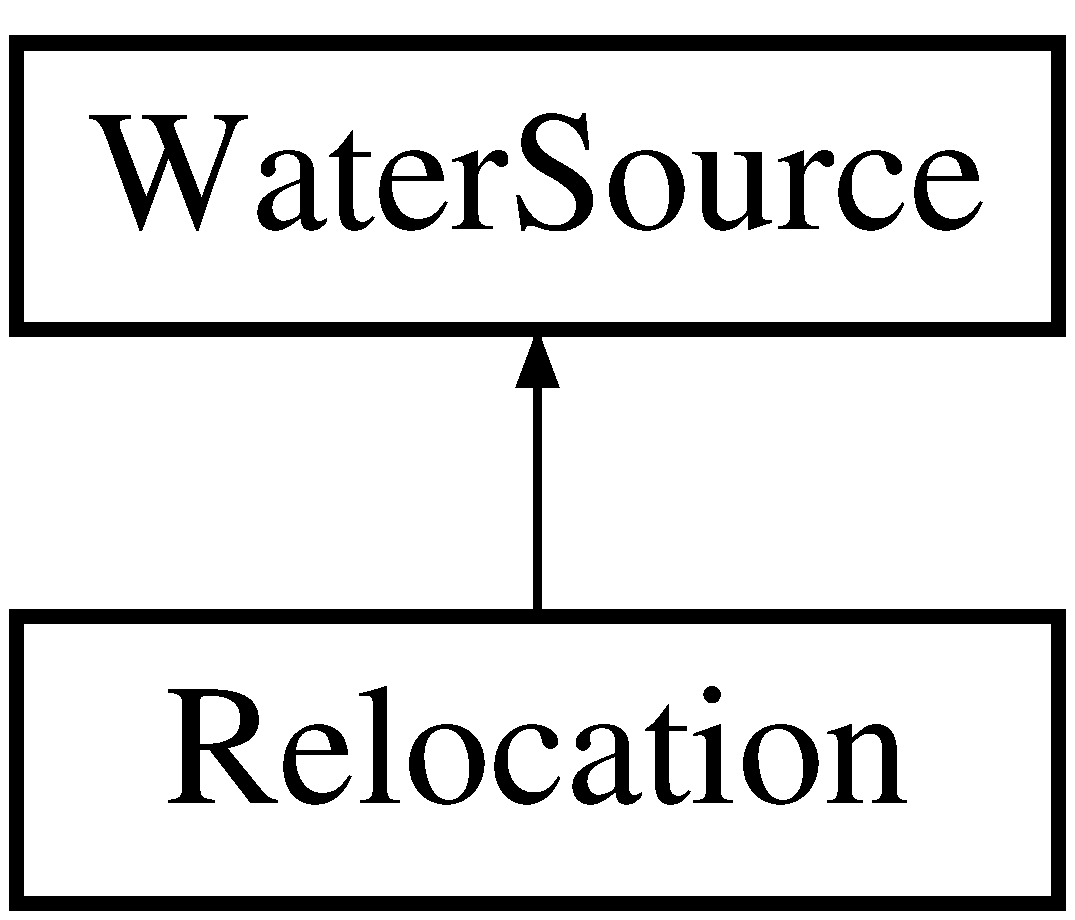
\includegraphics[height=2.000000cm]{classRelocation}
\end{center}
\end{figure}
\subsection*{Public Member Functions}
\begin{DoxyCompactItemize}
\item 
\mbox{\hyperlink{classRelocation_abeada1f0c797d8992c1e6a200b571574_abeada1f0c797d8992c1e6a200b571574}{Relocation}} (const char $\ast$\mbox{\hyperlink{classWaterSource_a846ea74c5b453d014f594d41fee8c765_a846ea74c5b453d014f594d41fee8c765}{name}}, const int \mbox{\hyperlink{classWaterSource_a6eafe5dfefd317877d1244e8a7c6e742_a6eafe5dfefd317877d1244e8a7c6e742}{id}}, unsigned long \mbox{\hyperlink{classRelocation_a61282254064f00641aaec667a7eb0652_a61282254064f00641aaec667a7eb0652}{parent\+\_\+reservoir\+\_\+\+ID}}, vector$<$ double $>$ $\ast$\mbox{\hyperlink{classWaterSource_a2f6655a80c4847fe039987255d9d998c_a2f6655a80c4847fe039987255d9d998c}{allocated\+\_\+fractions}}, vector$<$ int $>$ $\ast$\mbox{\hyperlink{classRelocation_ae426f390487b6b67f19bfbf556c922c2_ae426f390487b6b67f19bfbf556c922c2}{utilities\+\_\+with\+\_\+allocations}}, const vector$<$ double $>$ \&construction\+\_\+time\+\_\+range, double permitting\+\_\+period, \mbox{\hyperlink{classBond}{Bond}} \&bond)
\item 
\mbox{\hyperlink{classRelocation_a51eeb6a7d2b07940c2688b9b550145f0_a51eeb6a7d2b07940c2688b9b550145f0}{Relocation}} (const \mbox{\hyperlink{classRelocation}{Relocation}} \&relocation)
\item 
void \mbox{\hyperlink{classRelocation_af5c795c7b331b86b31c8bfa2ef9b6fe5_af5c795c7b331b86b31c8bfa2ef9b6fe5}{apply\+Continuity}} (int week, double \mbox{\hyperlink{classWaterSource_a7a69b2e9b6030f1035e6cf44d2918ee5_a7a69b2e9b6030f1035e6cf44d2918ee5}{upstream\+\_\+source\+\_\+inflow}}, double wastewater\+\_\+discharge, vector$<$ double $>$ \&demand\+\_\+outflow) override
\item 
unsigned long \mbox{\hyperlink{classRelocation_ae04b94d64c0ffd9a14dcdafdea551988_ae04b94d64c0ffd9a14dcdafdea551988}{get\+Parent\+\_\+reservoir\+\_\+\+ID}} () const
\end{DoxyCompactItemize}
\subsection*{Data Fields}
\begin{DoxyCompactItemize}
\item 
const unsigned long \mbox{\hyperlink{classRelocation_a61282254064f00641aaec667a7eb0652_a61282254064f00641aaec667a7eb0652}{parent\+\_\+reservoir\+\_\+\+ID}}
\item 
const vector$<$ double $>$ $\ast$ \mbox{\hyperlink{classRelocation_acc95d1be560fed2b4a1b4b2ae605ae67_acc95d1be560fed2b4a1b4b2ae605ae67}{new\+\_\+allocated\+\_\+fractions}}
\item 
const vector$<$ int $>$ $\ast$ \mbox{\hyperlink{classRelocation_ae426f390487b6b67f19bfbf556c922c2_ae426f390487b6b67f19bfbf556c922c2}{utilities\+\_\+with\+\_\+allocations}}
\end{DoxyCompactItemize}
\subsection*{Additional Inherited Members}


\subsection{Constructor \& Destructor Documentation}
\mbox{\Hypertarget{classRelocation_abeada1f0c797d8992c1e6a200b571574_abeada1f0c797d8992c1e6a200b571574}\label{classRelocation_abeada1f0c797d8992c1e6a200b571574_abeada1f0c797d8992c1e6a200b571574}} 
\index{Relocation@{Relocation}!Relocation@{Relocation}}
\index{Relocation@{Relocation}!Relocation@{Relocation}}
\subsubsection{\texorpdfstring{Relocation()}{Relocation()}\hspace{0.1cm}{\footnotesize\ttfamily [1/2]}}
{\footnotesize\ttfamily Relocation\+::\+Relocation (\begin{DoxyParamCaption}\item[{const char $\ast$}]{name,  }\item[{const int}]{id,  }\item[{unsigned long}]{parent\+\_\+reservoir\+\_\+\+ID,  }\item[{vector$<$ double $>$ $\ast$}]{allocated\+\_\+fractions,  }\item[{vector$<$ int $>$ $\ast$}]{utilities\+\_\+with\+\_\+allocations,  }\item[{const vector$<$ double $>$ \&}]{construction\+\_\+time\+\_\+range,  }\item[{double}]{permitting\+\_\+period,  }\item[{\mbox{\hyperlink{classBond}{Bond}} \&}]{bond }\end{DoxyParamCaption})}

\mbox{\Hypertarget{classRelocation_a51eeb6a7d2b07940c2688b9b550145f0_a51eeb6a7d2b07940c2688b9b550145f0}\label{classRelocation_a51eeb6a7d2b07940c2688b9b550145f0_a51eeb6a7d2b07940c2688b9b550145f0}} 
\index{Relocation@{Relocation}!Relocation@{Relocation}}
\index{Relocation@{Relocation}!Relocation@{Relocation}}
\subsubsection{\texorpdfstring{Relocation()}{Relocation()}\hspace{0.1cm}{\footnotesize\ttfamily [2/2]}}
{\footnotesize\ttfamily Relocation\+::\+Relocation (\begin{DoxyParamCaption}\item[{const \mbox{\hyperlink{classRelocation}{Relocation}} \&}]{relocation }\end{DoxyParamCaption})}

Copy constructor. 
\begin{DoxyParams}{Parameters}
{\em reservoir} & \\
\hline
\end{DoxyParams}


\subsection{Member Function Documentation}
\mbox{\Hypertarget{classRelocation_af5c795c7b331b86b31c8bfa2ef9b6fe5_af5c795c7b331b86b31c8bfa2ef9b6fe5}\label{classRelocation_af5c795c7b331b86b31c8bfa2ef9b6fe5_af5c795c7b331b86b31c8bfa2ef9b6fe5}} 
\index{Relocation@{Relocation}!apply\+Continuity@{apply\+Continuity}}
\index{apply\+Continuity@{apply\+Continuity}!Relocation@{Relocation}}
\subsubsection{\texorpdfstring{apply\+Continuity()}{applyContinuity()}}
{\footnotesize\ttfamily void Relocation\+::apply\+Continuity (\begin{DoxyParamCaption}\item[{int}]{week,  }\item[{double}]{upstream\+\_\+source\+\_\+inflow,  }\item[{double}]{wastewater\+\_\+discharge,  }\item[{vector$<$ double $>$ \&}]{demand\+\_\+outflow }\end{DoxyParamCaption})\hspace{0.3cm}{\ttfamily [override]}, {\ttfamily [virtual]}}



Implements \mbox{\hyperlink{classWaterSource_ac070445379fe706f65b977dade4f3fbc_ac070445379fe706f65b977dade4f3fbc}{Water\+Source}}.

\mbox{\Hypertarget{classRelocation_ae04b94d64c0ffd9a14dcdafdea551988_ae04b94d64c0ffd9a14dcdafdea551988}\label{classRelocation_ae04b94d64c0ffd9a14dcdafdea551988_ae04b94d64c0ffd9a14dcdafdea551988}} 
\index{Relocation@{Relocation}!get\+Parent\+\_\+reservoir\+\_\+\+ID@{get\+Parent\+\_\+reservoir\+\_\+\+ID}}
\index{get\+Parent\+\_\+reservoir\+\_\+\+ID@{get\+Parent\+\_\+reservoir\+\_\+\+ID}!Relocation@{Relocation}}
\subsubsection{\texorpdfstring{get\+Parent\+\_\+reservoir\+\_\+\+I\+D()}{getParent\_reservoir\_ID()}}
{\footnotesize\ttfamily unsigned long Relocation\+::get\+Parent\+\_\+reservoir\+\_\+\+ID (\begin{DoxyParamCaption}{ }\end{DoxyParamCaption}) const}



\subsection{Field Documentation}
\mbox{\Hypertarget{classRelocation_acc95d1be560fed2b4a1b4b2ae605ae67_acc95d1be560fed2b4a1b4b2ae605ae67}\label{classRelocation_acc95d1be560fed2b4a1b4b2ae605ae67_acc95d1be560fed2b4a1b4b2ae605ae67}} 
\index{Relocation@{Relocation}!new\+\_\+allocated\+\_\+fractions@{new\+\_\+allocated\+\_\+fractions}}
\index{new\+\_\+allocated\+\_\+fractions@{new\+\_\+allocated\+\_\+fractions}!Relocation@{Relocation}}
\subsubsection{\texorpdfstring{new\+\_\+allocated\+\_\+fractions}{new\_allocated\_fractions}}
{\footnotesize\ttfamily const vector$<$double$>$$\ast$ Relocation\+::new\+\_\+allocated\+\_\+fractions}

\mbox{\Hypertarget{classRelocation_a61282254064f00641aaec667a7eb0652_a61282254064f00641aaec667a7eb0652}\label{classRelocation_a61282254064f00641aaec667a7eb0652_a61282254064f00641aaec667a7eb0652}} 
\index{Relocation@{Relocation}!parent\+\_\+reservoir\+\_\+\+ID@{parent\+\_\+reservoir\+\_\+\+ID}}
\index{parent\+\_\+reservoir\+\_\+\+ID@{parent\+\_\+reservoir\+\_\+\+ID}!Relocation@{Relocation}}
\subsubsection{\texorpdfstring{parent\+\_\+reservoir\+\_\+\+ID}{parent\_reservoir\_ID}}
{\footnotesize\ttfamily const unsigned long Relocation\+::parent\+\_\+reservoir\+\_\+\+ID}

\mbox{\Hypertarget{classRelocation_ae426f390487b6b67f19bfbf556c922c2_ae426f390487b6b67f19bfbf556c922c2}\label{classRelocation_ae426f390487b6b67f19bfbf556c922c2_ae426f390487b6b67f19bfbf556c922c2}} 
\index{Relocation@{Relocation}!utilities\+\_\+with\+\_\+allocations@{utilities\+\_\+with\+\_\+allocations}}
\index{utilities\+\_\+with\+\_\+allocations@{utilities\+\_\+with\+\_\+allocations}!Relocation@{Relocation}}
\subsubsection{\texorpdfstring{utilities\+\_\+with\+\_\+allocations}{utilities\_with\_allocations}}
{\footnotesize\ttfamily const vector$<$int$>$$\ast$ Relocation\+::utilities\+\_\+with\+\_\+allocations}



The documentation for this class was generated from the following files\+:\begin{DoxyCompactItemize}
\item 
src/\+System\+Components/\+Water\+Sources/\mbox{\hyperlink{Relocation_8h}{Relocation.\+h}}\item 
src/\+System\+Components/\+Water\+Sources/\mbox{\hyperlink{Relocation_8cpp}{Relocation.\+cpp}}\end{DoxyCompactItemize}

\hypertarget{classReservoir}{}\section{Reservoir Class Reference}
\label{classReservoir}\index{Reservoir@{Reservoir}}


The {\ttfamily \mbox{\hyperlink{classReservoir}{Reservoir}}} class is a subclass of the main {\ttfamily \mbox{\hyperlink{classWaterSource}{Water\+Source}}} class. It represents a general reservoir object with a fixed or variable storage area curve.  




{\ttfamily \#include $<$Reservoir.\+h$>$}

Inheritance diagram for Reservoir\+:\begin{figure}[H]
\begin{center}
\leavevmode
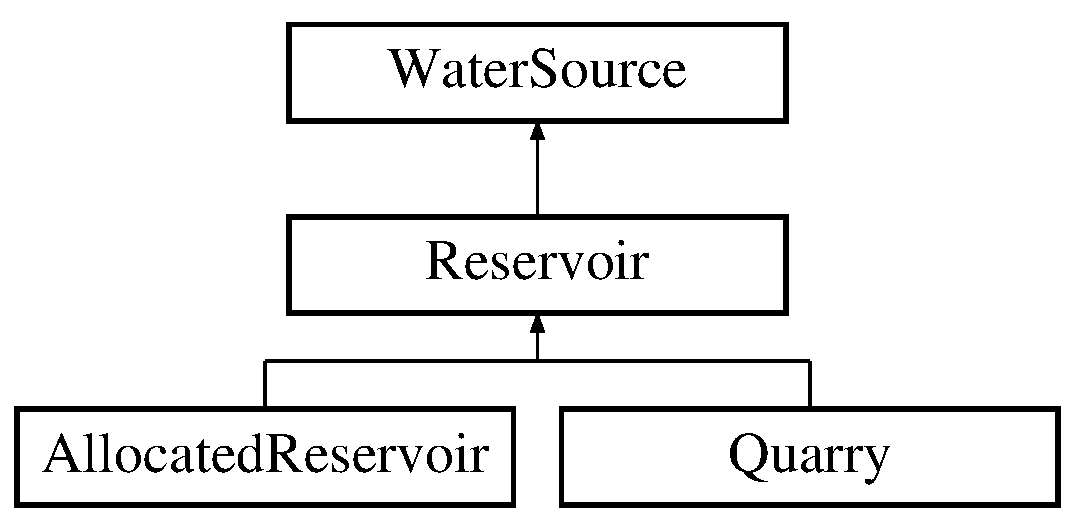
\includegraphics[height=3.000000cm]{classReservoir}
\end{center}
\end{figure}
\subsection*{Public Member Functions}
\begin{DoxyCompactItemize}
\item 
\mbox{\hyperlink{classReservoir_ac9803ae5446e4e9a2631ce66817004cf}{Reservoir}} (const char $\ast$\mbox{\hyperlink{classWaterSource_a846ea74c5b453d014f594d41fee8c765}{name}}, const int \mbox{\hyperlink{classWaterSource_a6eafe5dfefd317877d1244e8a7c6e742}{id}}, const vector$<$ \mbox{\hyperlink{classCatchment}{Catchment}} $\ast$$>$ \&\mbox{\hyperlink{classWaterSource_a8c18c34f23f8a06685c1d12f462ed830}{catchments}}, const double \mbox{\hyperlink{classWaterSource_a2ec257b415b248214a8bce7fc5267723}{capacity}}, const double max\+\_\+treatment\+\_\+capacity, \mbox{\hyperlink{classEvaporationSeries}{Evaporation\+Series}} \&\mbox{\hyperlink{classReservoir_a2d2d9b302c13703309bb798d24136810}{evaporation\+\_\+series}}, \mbox{\hyperlink{classDataSeries}{Data\+Series}} $\ast$\mbox{\hyperlink{classReservoir_a46bd5b750963dfa9a57b247fd77ab8ff}{storage\+\_\+area\+\_\+curve}}, int \mbox{\hyperlink{classWaterSource_afdd12c29fc74ea21dff1f1be9b8c2b7b}{source\+\_\+type}}=R\+E\+S\+E\+R\+V\+O\+IR)
\begin{DoxyCompactList}\small\item\em Constructs a basic \mbox{\hyperlink{classReservoir}{Reservoir}} object with a storage area curve. It also ensures that the last storage value in the storage area curve matches the reservoir\textquotesingle{}s capacity. \end{DoxyCompactList}\item 
\mbox{\hyperlink{classReservoir_a2e324b75aacc65d90b214ff7f62dfa89}{Reservoir}} (const char $\ast$\mbox{\hyperlink{classWaterSource_a846ea74c5b453d014f594d41fee8c765}{name}}, const int \mbox{\hyperlink{classWaterSource_a6eafe5dfefd317877d1244e8a7c6e742}{id}}, const vector$<$ \mbox{\hyperlink{classCatchment}{Catchment}} $\ast$$>$ \&\mbox{\hyperlink{classWaterSource_a8c18c34f23f8a06685c1d12f462ed830}{catchments}}, const double \mbox{\hyperlink{classWaterSource_a2ec257b415b248214a8bce7fc5267723}{capacity}}, const double max\+\_\+treatment\+\_\+capacity, \mbox{\hyperlink{classEvaporationSeries}{Evaporation\+Series}} \&\mbox{\hyperlink{classReservoir_a2d2d9b302c13703309bb798d24136810}{evaporation\+\_\+series}}, \mbox{\hyperlink{classDataSeries}{Data\+Series}} $\ast$\mbox{\hyperlink{classReservoir_a46bd5b750963dfa9a57b247fd77ab8ff}{storage\+\_\+area\+\_\+curve}}, const vector$<$ double $>$ \&construction\+\_\+time\+\_\+range, double permitting\+\_\+period, \mbox{\hyperlink{classBond}{Bond}} \&bond, int \mbox{\hyperlink{classWaterSource_afdd12c29fc74ea21dff1f1be9b8c2b7b}{source\+\_\+type}}=R\+E\+S\+E\+R\+V\+O\+IR)
\begin{DoxyCompactList}\small\item\em Constructs a \mbox{\hyperlink{classReservoir}{Reservoir}} object with a storage area curve, treatment capacity. Also includes financing, construction, and permitting information. \end{DoxyCompactList}\item 
\mbox{\hyperlink{classReservoir_a0a1041fc72df190bbc51d965ede96f49}{Reservoir}} (const char $\ast$\mbox{\hyperlink{classWaterSource_a846ea74c5b453d014f594d41fee8c765}{name}}, const int \mbox{\hyperlink{classWaterSource_a6eafe5dfefd317877d1244e8a7c6e742}{id}}, const vector$<$ \mbox{\hyperlink{classCatchment}{Catchment}} $\ast$$>$ \&\mbox{\hyperlink{classWaterSource_a8c18c34f23f8a06685c1d12f462ed830}{catchments}}, const double \mbox{\hyperlink{classWaterSource_a2ec257b415b248214a8bce7fc5267723}{capacity}}, const double max\+\_\+treatment\+\_\+capacity, \mbox{\hyperlink{classEvaporationSeries}{Evaporation\+Series}} \&\mbox{\hyperlink{classReservoir_a2d2d9b302c13703309bb798d24136810}{evaporation\+\_\+series}}, double storage\+\_\+area, int \mbox{\hyperlink{classWaterSource_afdd12c29fc74ea21dff1f1be9b8c2b7b}{source\+\_\+type}}=R\+E\+S\+E\+R\+V\+O\+IR)
\begin{DoxyCompactList}\small\item\em Constructs a \mbox{\hyperlink{classReservoir}{Reservoir}} object with a fixed storage area, treatment capacity, and evaporation data. \end{DoxyCompactList}\item 
\mbox{\hyperlink{classReservoir_a56409325d4554f8ef32a9c3605ece5c8}{Reservoir}} (const char $\ast$\mbox{\hyperlink{classWaterSource_a846ea74c5b453d014f594d41fee8c765}{name}}, const int \mbox{\hyperlink{classWaterSource_a6eafe5dfefd317877d1244e8a7c6e742}{id}}, const vector$<$ \mbox{\hyperlink{classCatchment}{Catchment}} $\ast$$>$ \&\mbox{\hyperlink{classWaterSource_a8c18c34f23f8a06685c1d12f462ed830}{catchments}}, const double \mbox{\hyperlink{classWaterSource_a2ec257b415b248214a8bce7fc5267723}{capacity}}, const double max\+\_\+treatment\+\_\+capacity, \mbox{\hyperlink{classEvaporationSeries}{Evaporation\+Series}} \&\mbox{\hyperlink{classReservoir_a2d2d9b302c13703309bb798d24136810}{evaporation\+\_\+series}}, double storage\+\_\+area, const vector$<$ double $>$ \&construction\+\_\+time\+\_\+range, double permitting\+\_\+period, \mbox{\hyperlink{classBond}{Bond}} \&bond, int \mbox{\hyperlink{classWaterSource_afdd12c29fc74ea21dff1f1be9b8c2b7b}{source\+\_\+type}}=R\+E\+S\+E\+R\+V\+O\+IR)
\begin{DoxyCompactList}\small\item\em Constructs a \mbox{\hyperlink{classReservoir}{Reservoir}} object with a fixed storage area, treatment capacity. Also includes financing, construction, and permitting information. \end{DoxyCompactList}\item 
\mbox{\hyperlink{classReservoir_a1a6f078a9565dcb65843d3575bdd4172}{Reservoir}} (const char $\ast$\mbox{\hyperlink{classWaterSource_a846ea74c5b453d014f594d41fee8c765}{name}}, const int \mbox{\hyperlink{classWaterSource_a6eafe5dfefd317877d1244e8a7c6e742}{id}}, const vector$<$ \mbox{\hyperlink{classCatchment}{Catchment}} $\ast$$>$ \&\mbox{\hyperlink{classWaterSource_a8c18c34f23f8a06685c1d12f462ed830}{catchments}}, const double \mbox{\hyperlink{classWaterSource_a2ec257b415b248214a8bce7fc5267723}{capacity}}, const double max\+\_\+treatment\+\_\+capacity, \mbox{\hyperlink{classEvaporationSeries}{Evaporation\+Series}} \&\mbox{\hyperlink{classReservoir_a2d2d9b302c13703309bb798d24136810}{evaporation\+\_\+series}}, \mbox{\hyperlink{classDataSeries}{Data\+Series}} $\ast$\mbox{\hyperlink{classReservoir_a46bd5b750963dfa9a57b247fd77ab8ff}{storage\+\_\+area\+\_\+curve}}, vector$<$ double $>$ $\ast$\mbox{\hyperlink{classWaterSource_aa73fe10cfc6579b2fb79529e1dde5140}{allocated\+\_\+treatment\+\_\+fractions}}, vector$<$ double $>$ $\ast$\mbox{\hyperlink{classWaterSource_a2f6655a80c4847fe039987255d9d998c}{allocated\+\_\+fractions}}, vector$<$ int $>$ $\ast$\mbox{\hyperlink{classWaterSource_ac345583fc2d0f7e1db31ee40244d7ace}{utilities\+\_\+with\+\_\+allocations}}, int \mbox{\hyperlink{classWaterSource_afdd12c29fc74ea21dff1f1be9b8c2b7b}{source\+\_\+type}}=R\+E\+S\+E\+R\+V\+O\+IR)
\begin{DoxyCompactList}\small\item\em Constructs a \mbox{\hyperlink{classReservoir}{Reservoir}} object with specified storage area curve. Includes additional details like treatment fractions and allocation details to connected utilities. \end{DoxyCompactList}\item 
\mbox{\hyperlink{classReservoir_a617f90b97899699d7e0dd97e7ebb34bc}{Reservoir}} (const char $\ast$\mbox{\hyperlink{classWaterSource_a846ea74c5b453d014f594d41fee8c765}{name}}, const int \mbox{\hyperlink{classWaterSource_a6eafe5dfefd317877d1244e8a7c6e742}{id}}, const vector$<$ \mbox{\hyperlink{classCatchment}{Catchment}} $\ast$$>$ \&\mbox{\hyperlink{classWaterSource_a8c18c34f23f8a06685c1d12f462ed830}{catchments}}, const double \mbox{\hyperlink{classWaterSource_a2ec257b415b248214a8bce7fc5267723}{capacity}}, const double max\+\_\+treatment\+\_\+capacity, \mbox{\hyperlink{classEvaporationSeries}{Evaporation\+Series}} \&\mbox{\hyperlink{classReservoir_a2d2d9b302c13703309bb798d24136810}{evaporation\+\_\+series}}, double storage\+\_\+area, vector$<$ double $>$ $\ast$\mbox{\hyperlink{classWaterSource_aa73fe10cfc6579b2fb79529e1dde5140}{allocated\+\_\+treatment\+\_\+fractions}}, vector$<$ double $>$ $\ast$\mbox{\hyperlink{classWaterSource_a2f6655a80c4847fe039987255d9d998c}{allocated\+\_\+fractions}}, vector$<$ int $>$ $\ast$\mbox{\hyperlink{classWaterSource_ac345583fc2d0f7e1db31ee40244d7ace}{utilities\+\_\+with\+\_\+allocations}}, int \mbox{\hyperlink{classWaterSource_afdd12c29fc74ea21dff1f1be9b8c2b7b}{source\+\_\+type}}=R\+E\+S\+E\+R\+V\+O\+IR)
\begin{DoxyCompactList}\small\item\em Constructs a \mbox{\hyperlink{classReservoir}{Reservoir}} object with specified storage area curve. Includes additional details like treatment fractions and allocation details to connected utilities. \end{DoxyCompactList}\item 
\mbox{\hyperlink{classReservoir_ac20659043afad4d2df49ce91e08f5dad}{Reservoir}} (const char $\ast$\mbox{\hyperlink{classWaterSource_a846ea74c5b453d014f594d41fee8c765}{name}}, const int \mbox{\hyperlink{classWaterSource_a6eafe5dfefd317877d1244e8a7c6e742}{id}}, const vector$<$ \mbox{\hyperlink{classCatchment}{Catchment}} $\ast$$>$ \&\mbox{\hyperlink{classWaterSource_a8c18c34f23f8a06685c1d12f462ed830}{catchments}}, const double \mbox{\hyperlink{classWaterSource_a2ec257b415b248214a8bce7fc5267723}{capacity}}, const double max\+\_\+treatment\+\_\+capacity, \mbox{\hyperlink{classEvaporationSeries}{Evaporation\+Series}} \&\mbox{\hyperlink{classReservoir_a2d2d9b302c13703309bb798d24136810}{evaporation\+\_\+series}}, \mbox{\hyperlink{classDataSeries}{Data\+Series}} $\ast$\mbox{\hyperlink{classReservoir_a46bd5b750963dfa9a57b247fd77ab8ff}{storage\+\_\+area\+\_\+curve}}, vector$<$ double $>$ $\ast$\mbox{\hyperlink{classWaterSource_aa73fe10cfc6579b2fb79529e1dde5140}{allocated\+\_\+treatment\+\_\+fractions}}, vector$<$ double $>$ $\ast$\mbox{\hyperlink{classWaterSource_a2f6655a80c4847fe039987255d9d998c}{allocated\+\_\+fractions}}, vector$<$ int $>$ $\ast$\mbox{\hyperlink{classWaterSource_ac345583fc2d0f7e1db31ee40244d7ace}{utilities\+\_\+with\+\_\+allocations}}, const vector$<$ double $>$ \&construction\+\_\+time\+\_\+range, double permitting\+\_\+period, \mbox{\hyperlink{classBond}{Bond}} \&bond, int \mbox{\hyperlink{classWaterSource_afdd12c29fc74ea21dff1f1be9b8c2b7b}{source\+\_\+type}}=R\+E\+S\+E\+R\+V\+O\+IR)
\begin{DoxyCompactList}\small\item\em Constructs a \mbox{\hyperlink{classReservoir}{Reservoir}} object with specified storage area curve. Includes additional details like treatment fractions and allocation details to connected utilities. Also includes financing, construction, and permitting information. \end{DoxyCompactList}\item 
\mbox{\hyperlink{classReservoir_a37ca7ba59d127fee6522c1ad545c9caf}{Reservoir}} (const char $\ast$\mbox{\hyperlink{classWaterSource_a846ea74c5b453d014f594d41fee8c765}{name}}, const int \mbox{\hyperlink{classWaterSource_a6eafe5dfefd317877d1244e8a7c6e742}{id}}, const vector$<$ \mbox{\hyperlink{classCatchment}{Catchment}} $\ast$$>$ \&\mbox{\hyperlink{classWaterSource_a8c18c34f23f8a06685c1d12f462ed830}{catchments}}, const double \mbox{\hyperlink{classWaterSource_a2ec257b415b248214a8bce7fc5267723}{capacity}}, const double max\+\_\+treatment\+\_\+capacity, \mbox{\hyperlink{classEvaporationSeries}{Evaporation\+Series}} \&\mbox{\hyperlink{classReservoir_a2d2d9b302c13703309bb798d24136810}{evaporation\+\_\+series}}, double storage\+\_\+area, vector$<$ double $>$ $\ast$\mbox{\hyperlink{classWaterSource_aa73fe10cfc6579b2fb79529e1dde5140}{allocated\+\_\+treatment\+\_\+fractions}}, vector$<$ double $>$ $\ast$\mbox{\hyperlink{classWaterSource_a2f6655a80c4847fe039987255d9d998c}{allocated\+\_\+fractions}}, vector$<$ int $>$ $\ast$\mbox{\hyperlink{classWaterSource_ac345583fc2d0f7e1db31ee40244d7ace}{utilities\+\_\+with\+\_\+allocations}}, const vector$<$ double $>$ \&construction\+\_\+time\+\_\+range, double permitting\+\_\+period, \mbox{\hyperlink{classBond}{Bond}} \&bond, int \mbox{\hyperlink{classWaterSource_afdd12c29fc74ea21dff1f1be9b8c2b7b}{source\+\_\+type}}=R\+E\+S\+E\+R\+V\+O\+IR)
\begin{DoxyCompactList}\small\item\em Constructs a \mbox{\hyperlink{classReservoir}{Reservoir}} object with fixed storage area. Includes additional details like treatment fractions and allocation details to connected utilities. Also includes financing, construction, and permitting information. \end{DoxyCompactList}\item 
\mbox{\hyperlink{classReservoir_a3fc46303b2846aa23bb52f0b69b9585c}{Reservoir}} (const \mbox{\hyperlink{classReservoir}{Reservoir}} \&reservoir)
\begin{DoxyCompactList}\small\item\em Copy constructor for creating a copy of an existing \mbox{\hyperlink{classReservoir}{Reservoir}} object. A new {\ttfamily \mbox{\hyperlink{classEvaporationSeries}{Evaporation\+Series}}} is created to ensure deep copying of the evaporation data. \end{DoxyCompactList}\item 
\mbox{\hyperlink{classReservoir}{Reservoir}} \& \mbox{\hyperlink{classReservoir_a8b43209f25276f279986d87b5a77c4f1}{operator=}} (const \mbox{\hyperlink{classReservoir}{Reservoir}} \&reservoir)
\begin{DoxyCompactList}\small\item\em Assignment operator for copying data from another \mbox{\hyperlink{classReservoir}{Reservoir}} object. \end{DoxyCompactList}\item 
\mbox{\hyperlink{classReservoir_a2f8bfdc73c7470185775a940fb3531de}{$\sim$\+Reservoir}} () override
\begin{DoxyCompactList}\small\item\em Destructor for the \mbox{\hyperlink{classReservoir}{Reservoir}} class. \end{DoxyCompactList}\item 
void \mbox{\hyperlink{classReservoir_a66929c055193785bc9d47bcdf0bc7445}{apply\+Continuity}} (int week, double \mbox{\hyperlink{classWaterSource_a7a69b2e9b6030f1035e6cf44d2918ee5}{upstream\+\_\+source\+\_\+inflow}}, double wastewater\+\_\+discharge, vector$<$ double $>$ \&demand\+\_\+outflow) override
\begin{DoxyCompactList}\small\item\em Applies continuity calculations for the reservoir over a given week. \end{DoxyCompactList}\item 
void \mbox{\hyperlink{classReservoir_ac6f64dd92c401e58095e7b125855041b}{set\+Online}} () override
\begin{DoxyCompactList}\small\item\em Marks the reservoir as online and initializes available volume. \end{DoxyCompactList}\item 
void \mbox{\hyperlink{classReservoir_ad1bb7aa46397719d09e0b6188b9bc28d}{set\+Realization}} (unsigned long r, vector$<$ double $>$ \&rdm\+\_\+factors) override
\begin{DoxyCompactList}\small\item\em Sets the realization for the reservoir and updates the evaporation series. \end{DoxyCompactList}\item 
double \mbox{\hyperlink{classReservoir_af86ffdaa2842a38b7f59e0360a1004a1}{get\+Area}} () const
\begin{DoxyCompactList}\small\item\em Returns the area of the reservoir. \end{DoxyCompactList}\end{DoxyCompactItemize}
\subsection*{Public Attributes}
\begin{DoxyCompactItemize}
\item 
const bool \mbox{\hyperlink{classReservoir_ad4b37aef4873071d1766baaccce5b8cf}{fixed\+\_\+area}}
\begin{DoxyCompactList}\small\item\em The fixed area of the reservoir. \end{DoxyCompactList}\item 
\mbox{\hyperlink{classEvaporationSeries}{Evaporation\+Series}} \mbox{\hyperlink{classReservoir_a2d2d9b302c13703309bb798d24136810}{evaporation\+\_\+series}}
\begin{DoxyCompactList}\small\item\em The \mbox{\hyperlink{classEvaporationSeries}{Evaporation\+Series}} object representing the evaporation series of the reservoir. \end{DoxyCompactList}\end{DoxyCompactItemize}
\subsection*{Protected Attributes}
\begin{DoxyCompactItemize}
\item 
\mbox{\hyperlink{classDataSeries}{Data\+Series}} $\ast$ \mbox{\hyperlink{classReservoir_a46bd5b750963dfa9a57b247fd77ab8ff}{storage\+\_\+area\+\_\+curve}}
\begin{DoxyCompactList}\small\item\em The \mbox{\hyperlink{classDataSeries}{Data\+Series}} object representing the storage area curve of the reservoir. \end{DoxyCompactList}\item 
double \mbox{\hyperlink{classReservoir_a57ab55e0dde9e29a4ff97de98b09e458}{area}} = N\+O\+N\+\_\+\+I\+N\+I\+T\+I\+A\+L\+I\+Z\+ED
\begin{DoxyCompactList}\small\item\em The area of the reservoir. \end{DoxyCompactList}\end{DoxyCompactItemize}
\subsection*{Additional Inherited Members}


\subsection{Detailed Description}
The {\ttfamily \mbox{\hyperlink{classReservoir}{Reservoir}}} class is a subclass of the main {\ttfamily \mbox{\hyperlink{classWaterSource}{Water\+Source}}} class. It represents a general reservoir object with a fixed or variable storage area curve. 

Created by bernardoct on 1/12/17. 

\subsection{Constructor \& Destructor Documentation}
\mbox{\Hypertarget{classReservoir_ac9803ae5446e4e9a2631ce66817004cf}\label{classReservoir_ac9803ae5446e4e9a2631ce66817004cf}} 
\index{Reservoir@{Reservoir}!Reservoir@{Reservoir}}
\index{Reservoir@{Reservoir}!Reservoir@{Reservoir}}
\subsubsection{\texorpdfstring{Reservoir()}{Reservoir()}\hspace{0.1cm}{\footnotesize\ttfamily [1/9]}}
{\footnotesize\ttfamily Reservoir\+::\+Reservoir (\begin{DoxyParamCaption}\item[{const char $\ast$}]{name,  }\item[{const int}]{id,  }\item[{const vector$<$ \mbox{\hyperlink{classCatchment}{Catchment}} $\ast$$>$ \&}]{catchments,  }\item[{const double}]{capacity,  }\item[{const double}]{max\+\_\+treatment\+\_\+capacity,  }\item[{\mbox{\hyperlink{classEvaporationSeries}{Evaporation\+Series}} \&}]{evaporation\+\_\+series,  }\item[{\mbox{\hyperlink{classDataSeries}{Data\+Series}} $\ast$}]{storage\+\_\+area\+\_\+curve,  }\item[{int}]{source\+\_\+type = {\ttfamily RESERVOIR} }\end{DoxyParamCaption})}



Constructs a basic \mbox{\hyperlink{classReservoir}{Reservoir}} object with a storage area curve. It also ensures that the last storage value in the storage area curve matches the reservoir\textquotesingle{}s capacity. 

Called for a reservoir that is already built and operational.


\begin{DoxyParams}{Parameters}
{\em name} & The name of the reservoir as a C-\/style string. \\
\hline
{\em id} & The unique identifier of the reservoir as an integer. \\
\hline
{\em catchments} & A vector of pointers to \mbox{\hyperlink{classCatchment}{Catchment}} objects representing the catchments linked to the reservoir. \\
\hline
{\em capacity} & The total storage capacity of the reservoir in cubic units. \\
\hline
{\em max\+\_\+treatment\+\_\+capacity} & The maximum treatment capacity of the reservoir in cubic units per time unit. \\
\hline
{\em evaporation\+\_\+series} & A reference to an \mbox{\hyperlink{classEvaporationSeries}{Evaporation\+Series}} object containing evaporation data for the reservoir. \\
\hline
{\em storage\+\_\+area\+\_\+curve} & A pointer to a \mbox{\hyperlink{classDataSeries}{Data\+Series}} object representing the storage area curve for the reservoir. \\
\hline
{\em source\+\_\+type} & The type of the source (e.\+g., a constant or specific reservoir type).\\
\hline
\end{DoxyParams}

\begin{DoxyExceptions}{Exceptions}
{\em invalid\+\_\+argument} & If the last storage value in the storage area curve does not match the reservoir\textquotesingle{}s capacity. \\
\hline
\end{DoxyExceptions}
\mbox{\Hypertarget{classReservoir_a2e324b75aacc65d90b214ff7f62dfa89}\label{classReservoir_a2e324b75aacc65d90b214ff7f62dfa89}} 
\index{Reservoir@{Reservoir}!Reservoir@{Reservoir}}
\index{Reservoir@{Reservoir}!Reservoir@{Reservoir}}
\subsubsection{\texorpdfstring{Reservoir()}{Reservoir()}\hspace{0.1cm}{\footnotesize\ttfamily [2/9]}}
{\footnotesize\ttfamily Reservoir\+::\+Reservoir (\begin{DoxyParamCaption}\item[{const char $\ast$}]{name,  }\item[{const int}]{id,  }\item[{const vector$<$ \mbox{\hyperlink{classCatchment}{Catchment}} $\ast$$>$ \&}]{catchments,  }\item[{const double}]{capacity,  }\item[{const double}]{max\+\_\+treatment\+\_\+capacity,  }\item[{\mbox{\hyperlink{classEvaporationSeries}{Evaporation\+Series}} \&}]{evaporation\+\_\+series,  }\item[{\mbox{\hyperlink{classDataSeries}{Data\+Series}} $\ast$}]{storage\+\_\+area\+\_\+curve,  }\item[{const vector$<$ double $>$ \&}]{construction\+\_\+time\+\_\+range,  }\item[{double}]{permitting\+\_\+period,  }\item[{\mbox{\hyperlink{classBond}{Bond}} \&}]{bond,  }\item[{int}]{source\+\_\+type = {\ttfamily RESERVOIR} }\end{DoxyParamCaption})}



Constructs a \mbox{\hyperlink{classReservoir}{Reservoir}} object with a storage area curve, treatment capacity. Also includes financing, construction, and permitting information. 

Called when the reservoir does not yet exist at the beginning of the simulation.

This function initializes a \mbox{\hyperlink{classReservoir}{Reservoir}} object with parameters such as the name, ID, catchments, capacity, maximum treatment capacity, evaporation series, storage area curve, and other construction and permitting details. It also ensures that the last storage value in the storage area curve matches the reservoir\textquotesingle{}s capacity.


\begin{DoxyParams}{Parameters}
{\em name} & The name of the reservoir as a C-\/style string. \\
\hline
{\em id} & The unique identifier of the reservoir as an integer. \\
\hline
{\em catchments} & A vector of pointers to \mbox{\hyperlink{classCatchment}{Catchment}} objects representing the catchments linked to the reservoir. \\
\hline
{\em capacity} & The total storage capacity of the reservoir in cubic units. \\
\hline
{\em max\+\_\+treatment\+\_\+capacity} & The maximum treatment capacity of the reservoir in cubic units per time unit. \\
\hline
{\em evaporation\+\_\+series} & A reference to an \mbox{\hyperlink{classEvaporationSeries}{Evaporation\+Series}} object containing evaporation data for the reservoir. \\
\hline
{\em storage\+\_\+area\+\_\+curve} & A pointer to a \mbox{\hyperlink{classDataSeries}{Data\+Series}} object representing the storage area curve for the reservoir. \\
\hline
{\em construction\+\_\+time\+\_\+range} & A vector of doubles representing the start and end times of the construction period. \\
\hline
{\em permitting\+\_\+period} & The permitting period for the reservoir in time units. \\
\hline
{\em bond} & A reference to a \mbox{\hyperlink{classBond}{Bond}} object representing the financial bond associated with the reservoir. \\
\hline
{\em source\+\_\+type} & The type of the source (e.\+g., a constant or specific reservoir type).\\
\hline
\end{DoxyParams}

\begin{DoxyExceptions}{Exceptions}
{\em invalid\+\_\+argument} & If the last storage value in the storage area curve does not match the reservoir\textquotesingle{}s capacity. \\
\hline
\end{DoxyExceptions}
\mbox{\Hypertarget{classReservoir_a0a1041fc72df190bbc51d965ede96f49}\label{classReservoir_a0a1041fc72df190bbc51d965ede96f49}} 
\index{Reservoir@{Reservoir}!Reservoir@{Reservoir}}
\index{Reservoir@{Reservoir}!Reservoir@{Reservoir}}
\subsubsection{\texorpdfstring{Reservoir()}{Reservoir()}\hspace{0.1cm}{\footnotesize\ttfamily [3/9]}}
{\footnotesize\ttfamily Reservoir\+::\+Reservoir (\begin{DoxyParamCaption}\item[{const char $\ast$}]{name,  }\item[{const int}]{id,  }\item[{const vector$<$ \mbox{\hyperlink{classCatchment}{Catchment}} $\ast$$>$ \&}]{catchments,  }\item[{const double}]{capacity,  }\item[{const double}]{max\+\_\+treatment\+\_\+capacity,  }\item[{\mbox{\hyperlink{classEvaporationSeries}{Evaporation\+Series}} \&}]{evaporation\+\_\+series,  }\item[{double}]{storage\+\_\+area,  }\item[{int}]{source\+\_\+type = {\ttfamily RESERVOIR} }\end{DoxyParamCaption})}



Constructs a \mbox{\hyperlink{classReservoir}{Reservoir}} object with a fixed storage area, treatment capacity, and evaporation data. 

Called for a reservoir that is already built and operational.


\begin{DoxyParams}{Parameters}
{\em name} & The name of the reservoir as a C-\/style string. \\
\hline
{\em id} & The unique identifier of the reservoir as an integer. \\
\hline
{\em catchments} & A vector of pointers to \mbox{\hyperlink{classCatchment}{Catchment}} objects representing the catchments linked to the reservoir. \\
\hline
{\em capacity} & The total storage capacity of the reservoir in cubic units. \\
\hline
{\em max\+\_\+treatment\+\_\+capacity} & The maximum treatment capacity of the reservoir in cubic units per time unit. \\
\hline
{\em evaporation\+\_\+series} & A reference to an \mbox{\hyperlink{classEvaporationSeries}{Evaporation\+Series}} object containing evaporation data for the reservoir. \\
\hline
{\em storage\+\_\+area} & The area of the reservoir in square units. \\
\hline
{\em source\+\_\+type} & The type of the source (e.\+g., a constant or specific reservoir type). \\
\hline
\end{DoxyParams}
\mbox{\Hypertarget{classReservoir_a56409325d4554f8ef32a9c3605ece5c8}\label{classReservoir_a56409325d4554f8ef32a9c3605ece5c8}} 
\index{Reservoir@{Reservoir}!Reservoir@{Reservoir}}
\index{Reservoir@{Reservoir}!Reservoir@{Reservoir}}
\subsubsection{\texorpdfstring{Reservoir()}{Reservoir()}\hspace{0.1cm}{\footnotesize\ttfamily [4/9]}}
{\footnotesize\ttfamily Reservoir\+::\+Reservoir (\begin{DoxyParamCaption}\item[{const char $\ast$}]{name,  }\item[{const int}]{id,  }\item[{const vector$<$ \mbox{\hyperlink{classCatchment}{Catchment}} $\ast$$>$ \&}]{catchments,  }\item[{const double}]{capacity,  }\item[{const double}]{max\+\_\+treatment\+\_\+capacity,  }\item[{\mbox{\hyperlink{classEvaporationSeries}{Evaporation\+Series}} \&}]{evaporation\+\_\+series,  }\item[{double}]{storage\+\_\+area,  }\item[{const vector$<$ double $>$ \&}]{construction\+\_\+time\+\_\+range,  }\item[{double}]{permitting\+\_\+period,  }\item[{\mbox{\hyperlink{classBond}{Bond}} \&}]{bond,  }\item[{int}]{source\+\_\+type = {\ttfamily RESERVOIR} }\end{DoxyParamCaption})}



Constructs a \mbox{\hyperlink{classReservoir}{Reservoir}} object with a fixed storage area, treatment capacity. Also includes financing, construction, and permitting information. 

Called when the reservoir does not yet exist at the beginning of the simulation.

This function initializes a \mbox{\hyperlink{classReservoir}{Reservoir}} object with parameters such as the name, ID, catchments, capacity, maximum treatment capacity, evaporation series, storage area curve, and other construction and permitting details. It also ensures that the last storage value in the storage area curve matches the reservoir\textquotesingle{}s capacity.


\begin{DoxyParams}{Parameters}
{\em name} & The name of the reservoir as a C-\/style string. \\
\hline
{\em id} & The unique identifier of the reservoir as an integer. \\
\hline
{\em catchments} & A vector of pointers to \mbox{\hyperlink{classCatchment}{Catchment}} objects representing the catchments linked to the reservoir. \\
\hline
{\em capacity} & The total storage capacity of the reservoir in cubic units. \\
\hline
{\em max\+\_\+treatment\+\_\+capacity} & The maximum treatment capacity of the reservoir in cubic units per time unit. \\
\hline
{\em evaporation\+\_\+series} & A reference to an \mbox{\hyperlink{classEvaporationSeries}{Evaporation\+Series}} object containing evaporation data for the reservoir. \\
\hline
{\em storage\+\_\+area\+\_\+curve} & A pointer to a \mbox{\hyperlink{classDataSeries}{Data\+Series}} object representing the storage area curve for the reservoir. \\
\hline
{\em construction\+\_\+time\+\_\+range} & A vector of doubles representing the start and end times of the construction period. \\
\hline
{\em permitting\+\_\+period} & The permitting period for the reservoir in time units. \\
\hline
{\em bond} & A reference to a \mbox{\hyperlink{classBond}{Bond}} object representing the financial bond associated with the reservoir. \\
\hline
{\em source\+\_\+type} & The type of the source (e.\+g., a constant or specific reservoir type).\\
\hline
\end{DoxyParams}

\begin{DoxyExceptions}{Exceptions}
{\em invalid\+\_\+argument} & If the last storage value in the storage area curve does not match the reservoir\textquotesingle{}s capacity. \\
\hline
\end{DoxyExceptions}
\mbox{\Hypertarget{classReservoir_a1a6f078a9565dcb65843d3575bdd4172}\label{classReservoir_a1a6f078a9565dcb65843d3575bdd4172}} 
\index{Reservoir@{Reservoir}!Reservoir@{Reservoir}}
\index{Reservoir@{Reservoir}!Reservoir@{Reservoir}}
\subsubsection{\texorpdfstring{Reservoir()}{Reservoir()}\hspace{0.1cm}{\footnotesize\ttfamily [5/9]}}
{\footnotesize\ttfamily Reservoir\+::\+Reservoir (\begin{DoxyParamCaption}\item[{const char $\ast$}]{name,  }\item[{const int}]{id,  }\item[{const vector$<$ \mbox{\hyperlink{classCatchment}{Catchment}} $\ast$$>$ \&}]{catchments,  }\item[{const double}]{capacity,  }\item[{const double}]{max\+\_\+treatment\+\_\+capacity,  }\item[{\mbox{\hyperlink{classEvaporationSeries}{Evaporation\+Series}} \&}]{evaporation\+\_\+series,  }\item[{\mbox{\hyperlink{classDataSeries}{Data\+Series}} $\ast$}]{storage\+\_\+area\+\_\+curve,  }\item[{vector$<$ double $>$ $\ast$}]{allocated\+\_\+treatment\+\_\+fractions,  }\item[{vector$<$ double $>$ $\ast$}]{allocated\+\_\+fractions,  }\item[{vector$<$ int $>$ $\ast$}]{utilities\+\_\+with\+\_\+allocations,  }\item[{int}]{source\+\_\+type = {\ttfamily RESERVOIR} }\end{DoxyParamCaption})}



Constructs a \mbox{\hyperlink{classReservoir}{Reservoir}} object with specified storage area curve. Includes additional details like treatment fractions and allocation details to connected utilities. 

Called for a reservoir that is already built and operational.


\begin{DoxyParams}{Parameters}
{\em name} & The name of the reservoir as a C-\/style string. \\
\hline
{\em id} & The unique identifier of the reservoir as an integer. \\
\hline
{\em catchments} & A vector of pointers to \mbox{\hyperlink{classCatchment}{Catchment}} objects representing the catchments linked to the reservoir. \\
\hline
{\em capacity} & The total storage capacity of the reservoir in cubic units. \\
\hline
{\em max\+\_\+treatment\+\_\+capacity} & The maximum treatment capacity of the reservoir in cubic units per time unit. \\
\hline
{\em evaporation\+\_\+series} & A reference to an \mbox{\hyperlink{classEvaporationSeries}{Evaporation\+Series}} object containing evaporation data for the reservoir. \\
\hline
{\em storage\+\_\+area\+\_\+curve} & A pointer to a \mbox{\hyperlink{classDataSeries}{Data\+Series}} object representing the storage area curve for the reservoir. \\
\hline
{\em allocated\+\_\+treatment\+\_\+fractions} & A pointer to a vector of treatment fractions allocated to utilities. \\
\hline
{\em allocated\+\_\+fractions} & A pointer to a vector of fractions allocated to utilities. \\
\hline
{\em utilities\+\_\+with\+\_\+allocations} & A pointer to a vector of integers representing the utilities that have allocations. \\
\hline
{\em source\+\_\+type} & The type of the source (e.\+g., a constant or specific reservoir type).\\
\hline
\end{DoxyParams}

\begin{DoxyExceptions}{Exceptions}
{\em invalid\+\_\+argument} & If the last storage value in the storage area curve does not match the reservoir\textquotesingle{}s capacity. \\
\hline
\end{DoxyExceptions}
\mbox{\Hypertarget{classReservoir_a617f90b97899699d7e0dd97e7ebb34bc}\label{classReservoir_a617f90b97899699d7e0dd97e7ebb34bc}} 
\index{Reservoir@{Reservoir}!Reservoir@{Reservoir}}
\index{Reservoir@{Reservoir}!Reservoir@{Reservoir}}
\subsubsection{\texorpdfstring{Reservoir()}{Reservoir()}\hspace{0.1cm}{\footnotesize\ttfamily [6/9]}}
{\footnotesize\ttfamily Reservoir\+::\+Reservoir (\begin{DoxyParamCaption}\item[{const char $\ast$}]{name,  }\item[{const int}]{id,  }\item[{const vector$<$ \mbox{\hyperlink{classCatchment}{Catchment}} $\ast$$>$ \&}]{catchments,  }\item[{const double}]{capacity,  }\item[{const double}]{max\+\_\+treatment\+\_\+capacity,  }\item[{\mbox{\hyperlink{classEvaporationSeries}{Evaporation\+Series}} \&}]{evaporation\+\_\+series,  }\item[{double}]{storage\+\_\+area,  }\item[{vector$<$ double $>$ $\ast$}]{allocated\+\_\+treatment\+\_\+fractions,  }\item[{vector$<$ double $>$ $\ast$}]{allocated\+\_\+fractions,  }\item[{vector$<$ int $>$ $\ast$}]{utilities\+\_\+with\+\_\+allocations,  }\item[{int}]{source\+\_\+type = {\ttfamily RESERVOIR} }\end{DoxyParamCaption})}



Constructs a \mbox{\hyperlink{classReservoir}{Reservoir}} object with specified storage area curve. Includes additional details like treatment fractions and allocation details to connected utilities. 

Called for a reservoir that is already built and operational.


\begin{DoxyParams}{Parameters}
{\em name} & The name of the reservoir as a C-\/style string. \\
\hline
{\em id} & The unique identifier of the reservoir as an integer. \\
\hline
{\em catchments} & A vector of pointers to \mbox{\hyperlink{classCatchment}{Catchment}} objects representing the catchments linked to the reservoir. \\
\hline
{\em capacity} & The total storage capacity of the reservoir in cubic units. \\
\hline
{\em max\+\_\+treatment\+\_\+capacity} & The maximum treatment capacity of the reservoir in cubic units per time unit. \\
\hline
{\em evaporation\+\_\+series} & A reference to an \mbox{\hyperlink{classEvaporationSeries}{Evaporation\+Series}} object containing evaporation data for the reservoir. \\
\hline
{\em storage\+\_\+area} & The area of the reservoir in square units. \\
\hline
{\em allocated\+\_\+treatment\+\_\+fractions} & A pointer to a vector of treatment fractions allocated to utilities. \\
\hline
{\em allocated\+\_\+fractions} & A pointer to a vector of fractions allocated to utilities. \\
\hline
{\em utilities\+\_\+with\+\_\+allocations} & A pointer to a vector of integers representing the utilities that have allocations. \\
\hline
{\em source\+\_\+type} & The type of the source (e.\+g., a constant or specific reservoir type). \\
\hline
\end{DoxyParams}
\mbox{\Hypertarget{classReservoir_ac20659043afad4d2df49ce91e08f5dad}\label{classReservoir_ac20659043afad4d2df49ce91e08f5dad}} 
\index{Reservoir@{Reservoir}!Reservoir@{Reservoir}}
\index{Reservoir@{Reservoir}!Reservoir@{Reservoir}}
\subsubsection{\texorpdfstring{Reservoir()}{Reservoir()}\hspace{0.1cm}{\footnotesize\ttfamily [7/9]}}
{\footnotesize\ttfamily Reservoir\+::\+Reservoir (\begin{DoxyParamCaption}\item[{const char $\ast$}]{name,  }\item[{const int}]{id,  }\item[{const vector$<$ \mbox{\hyperlink{classCatchment}{Catchment}} $\ast$$>$ \&}]{catchments,  }\item[{const double}]{capacity,  }\item[{const double}]{max\+\_\+treatment\+\_\+capacity,  }\item[{\mbox{\hyperlink{classEvaporationSeries}{Evaporation\+Series}} \&}]{evaporation\+\_\+series,  }\item[{\mbox{\hyperlink{classDataSeries}{Data\+Series}} $\ast$}]{storage\+\_\+area\+\_\+curve,  }\item[{vector$<$ double $>$ $\ast$}]{allocated\+\_\+treatment\+\_\+fractions,  }\item[{vector$<$ double $>$ $\ast$}]{allocated\+\_\+fractions,  }\item[{vector$<$ int $>$ $\ast$}]{utilities\+\_\+with\+\_\+allocations,  }\item[{const vector$<$ double $>$ \&}]{construction\+\_\+time\+\_\+range,  }\item[{double}]{permitting\+\_\+period,  }\item[{\mbox{\hyperlink{classBond}{Bond}} \&}]{bond,  }\item[{int}]{source\+\_\+type = {\ttfamily RESERVOIR} }\end{DoxyParamCaption})}



Constructs a \mbox{\hyperlink{classReservoir}{Reservoir}} object with specified storage area curve. Includes additional details like treatment fractions and allocation details to connected utilities. Also includes financing, construction, and permitting information. 

Called when the reservoir does not yet exist at the beginning of the simulation.


\begin{DoxyParams}{Parameters}
{\em name} & The name of the reservoir as a C-\/style string. \\
\hline
{\em id} & The unique identifier of the reservoir as an integer. \\
\hline
{\em catchments} & A vector of pointers to \mbox{\hyperlink{classCatchment}{Catchment}} objects representing the catchments linked to the reservoir. \\
\hline
{\em capacity} & The total storage capacity of the reservoir in cubic units. \\
\hline
{\em max\+\_\+treatment\+\_\+capacity} & The maximum treatment capacity of the reservoir in cubic units per time unit. \\
\hline
{\em evaporation\+\_\+series} & A reference to an \mbox{\hyperlink{classEvaporationSeries}{Evaporation\+Series}} object containing evaporation data for the reservoir. \\
\hline
{\em storage\+\_\+area\+\_\+curve} & A pointer to a \mbox{\hyperlink{classDataSeries}{Data\+Series}} object representing the storage area curve for the reservoir. \\
\hline
{\em allocated\+\_\+treatment\+\_\+fractions} & A pointer to a vector of treatment fractions allocated to utilities. \\
\hline
{\em allocated\+\_\+fractions} & A pointer to a vector of fractions allocated to utilities. \\
\hline
{\em utilities\+\_\+with\+\_\+allocations} & A pointer to a vector of integers representing the utilities that have allocations. \\
\hline
{\em construction\+\_\+time\+\_\+range} & A vector of doubles representing the start and end times of the construction period. \\
\hline
{\em permitting\+\_\+period} & The permitting period for the reservoir in time units. \\
\hline
{\em bond} & A reference to a \mbox{\hyperlink{classBond}{Bond}} object representing the financial bond associated with the reservoir. \\
\hline
{\em source\+\_\+type} & The type of the source (e.\+g., a constant or specific reservoir type).\\
\hline
\end{DoxyParams}

\begin{DoxyExceptions}{Exceptions}
{\em invalid\+\_\+argument} & If the last storage value in the storage area curve does not match the reservoir\textquotesingle{}s capacity. \\
\hline
\end{DoxyExceptions}
\mbox{\Hypertarget{classReservoir_a37ca7ba59d127fee6522c1ad545c9caf}\label{classReservoir_a37ca7ba59d127fee6522c1ad545c9caf}} 
\index{Reservoir@{Reservoir}!Reservoir@{Reservoir}}
\index{Reservoir@{Reservoir}!Reservoir@{Reservoir}}
\subsubsection{\texorpdfstring{Reservoir()}{Reservoir()}\hspace{0.1cm}{\footnotesize\ttfamily [8/9]}}
{\footnotesize\ttfamily Reservoir\+::\+Reservoir (\begin{DoxyParamCaption}\item[{const char $\ast$}]{name,  }\item[{const int}]{id,  }\item[{const vector$<$ \mbox{\hyperlink{classCatchment}{Catchment}} $\ast$$>$ \&}]{catchments,  }\item[{const double}]{capacity,  }\item[{const double}]{max\+\_\+treatment\+\_\+capacity,  }\item[{\mbox{\hyperlink{classEvaporationSeries}{Evaporation\+Series}} \&}]{evaporation\+\_\+series,  }\item[{double}]{storage\+\_\+area,  }\item[{vector$<$ double $>$ $\ast$}]{allocated\+\_\+treatment\+\_\+fractions,  }\item[{vector$<$ double $>$ $\ast$}]{allocated\+\_\+fractions,  }\item[{vector$<$ int $>$ $\ast$}]{utilities\+\_\+with\+\_\+allocations,  }\item[{const vector$<$ double $>$ \&}]{construction\+\_\+time\+\_\+range,  }\item[{double}]{permitting\+\_\+period,  }\item[{\mbox{\hyperlink{classBond}{Bond}} \&}]{bond,  }\item[{int}]{source\+\_\+type = {\ttfamily RESERVOIR} }\end{DoxyParamCaption})}



Constructs a \mbox{\hyperlink{classReservoir}{Reservoir}} object with fixed storage area. Includes additional details like treatment fractions and allocation details to connected utilities. Also includes financing, construction, and permitting information. 

Called when the reservoir does not yet exist at the beginning of the simulation.


\begin{DoxyParams}{Parameters}
{\em name} & The name of the reservoir as a C-\/style string. \\
\hline
{\em id} & The unique identifier of the reservoir as an integer. \\
\hline
{\em catchments} & A vector of pointers to \mbox{\hyperlink{classCatchment}{Catchment}} objects representing the catchments linked to the reservoir. \\
\hline
{\em capacity} & The total storage capacity of the reservoir in cubic units. \\
\hline
{\em max\+\_\+treatment\+\_\+capacity} & The maximum treatment capacity of the reservoir in cubic units per time unit. \\
\hline
{\em evaporation\+\_\+series} & A reference to an \mbox{\hyperlink{classEvaporationSeries}{Evaporation\+Series}} object containing evaporation data for the reservoir. \\
\hline
{\em storage\+\_\+area} & The area of the reservoir in square units. \\
\hline
{\em allocated\+\_\+treatment\+\_\+fractions} & A pointer to a vector of treatment fractions allocated to utilities. \\
\hline
{\em allocated\+\_\+fractions} & A pointer to a vector of fractions allocated to utilities. \\
\hline
{\em utilities\+\_\+with\+\_\+allocations} & A pointer to a vector of integers representing the utilities that have allocations. \\
\hline
{\em construction\+\_\+time\+\_\+range} & A vector of doubles representing the start and end times of the construction period. \\
\hline
{\em permitting\+\_\+period} & The permitting period for the reservoir in time units. \\
\hline
{\em bond} & A reference to a \mbox{\hyperlink{classBond}{Bond}} object representing the financial bond associated with the reservoir. \\
\hline
{\em source\+\_\+type} & The type of the source (e.\+g., a constant or specific reservoir type).\\
\hline
\end{DoxyParams}

\begin{DoxyExceptions}{Exceptions}
{\em invalid\+\_\+argument} & If the last storage value in the storage area curve does not match the reservoir\textquotesingle{}s capacity. \\
\hline
\end{DoxyExceptions}
\mbox{\Hypertarget{classReservoir_a3fc46303b2846aa23bb52f0b69b9585c}\label{classReservoir_a3fc46303b2846aa23bb52f0b69b9585c}} 
\index{Reservoir@{Reservoir}!Reservoir@{Reservoir}}
\index{Reservoir@{Reservoir}!Reservoir@{Reservoir}}
\subsubsection{\texorpdfstring{Reservoir()}{Reservoir()}\hspace{0.1cm}{\footnotesize\ttfamily [9/9]}}
{\footnotesize\ttfamily Reservoir\+::\+Reservoir (\begin{DoxyParamCaption}\item[{const \mbox{\hyperlink{classReservoir}{Reservoir}} \&}]{reservoir }\end{DoxyParamCaption})}



Copy constructor for creating a copy of an existing \mbox{\hyperlink{classReservoir}{Reservoir}} object. A new {\ttfamily \mbox{\hyperlink{classEvaporationSeries}{Evaporation\+Series}}} is created to ensure deep copying of the evaporation data. 


\begin{DoxyParams}{Parameters}
{\em reservoir} & The {\ttfamily \mbox{\hyperlink{classReservoir}{Reservoir}}} object to copy. \\
\hline
\end{DoxyParams}
\mbox{\Hypertarget{classReservoir_a2f8bfdc73c7470185775a940fb3531de}\label{classReservoir_a2f8bfdc73c7470185775a940fb3531de}} 
\index{Reservoir@{Reservoir}!````~Reservoir@{$\sim$\+Reservoir}}
\index{````~Reservoir@{$\sim$\+Reservoir}!Reservoir@{Reservoir}}
\subsubsection{\texorpdfstring{$\sim$\+Reservoir()}{~Reservoir()}}
{\footnotesize\ttfamily Reservoir\+::$\sim$\+Reservoir (\begin{DoxyParamCaption}{ }\end{DoxyParamCaption})\hspace{0.3cm}{\ttfamily [override]}}



Destructor for the \mbox{\hyperlink{classReservoir}{Reservoir}} class. 

This destructor is the default destructor for the {\ttfamily \mbox{\hyperlink{classReservoir}{Reservoir}}} class and overrides the corresponding function in the base class. It ensures proper cleanup of any dynamically allocated resources when a {\ttfamily \mbox{\hyperlink{classReservoir}{Reservoir}}} object is destroyed. 

\subsection{Member Function Documentation}
\mbox{\Hypertarget{classReservoir_a66929c055193785bc9d47bcdf0bc7445}\label{classReservoir_a66929c055193785bc9d47bcdf0bc7445}} 
\index{Reservoir@{Reservoir}!apply\+Continuity@{apply\+Continuity}}
\index{apply\+Continuity@{apply\+Continuity}!Reservoir@{Reservoir}}
\subsubsection{\texorpdfstring{apply\+Continuity()}{applyContinuity()}}
{\footnotesize\ttfamily void Reservoir\+::apply\+Continuity (\begin{DoxyParamCaption}\item[{int}]{week,  }\item[{double}]{upstream\+\_\+source\+\_\+inflow,  }\item[{double}]{wastewater\+\_\+discharge,  }\item[{vector$<$ double $>$ \&}]{demand\+\_\+outflow }\end{DoxyParamCaption})\hspace{0.3cm}{\ttfamily [override]}, {\ttfamily [virtual]}}



Applies continuity calculations for the reservoir over a given week. 

This function calculates the new stored volume and outflow for the reservoir based on the continuity equation, taking into account inflows, demand outflows, evaporation, and spillage. It also updates various internal state variables like total demand, available volume, and total outflow.

This function overrides the {\ttfamily apply\+Continuity} function in the base class {\ttfamily \mbox{\hyperlink{classWaterSource}{Water\+Source}}}.


\begin{DoxyParams}{Parameters}
{\em week} & The week for which continuity calculations are performed. \\
\hline
{\em upstream\+\_\+source\+\_\+inflow} & The inflow from upstream sources. \\
\hline
{\em wastewater\+\_\+inflow} & The inflow from wastewater sources. \\
\hline
{\em demand\+\_\+outflow} & A vector of demand outflows for the week. \\
\hline
\end{DoxyParams}


Implements \mbox{\hyperlink{classWaterSource_ac070445379fe706f65b977dade4f3fbc}{Water\+Source}}.

\mbox{\Hypertarget{classReservoir_af86ffdaa2842a38b7f59e0360a1004a1}\label{classReservoir_af86ffdaa2842a38b7f59e0360a1004a1}} 
\index{Reservoir@{Reservoir}!get\+Area@{get\+Area}}
\index{get\+Area@{get\+Area}!Reservoir@{Reservoir}}
\subsubsection{\texorpdfstring{get\+Area()}{getArea()}}
{\footnotesize\ttfamily double Reservoir\+::get\+Area (\begin{DoxyParamCaption}{ }\end{DoxyParamCaption}) const}



Returns the area of the reservoir. 

This function retrieves the area of the reservoir, which is used to calculate various hydrological properties related to the reservoir\textquotesingle{}s size.

\begin{DoxyReturn}{Returns}
The area of the reservoir as a {\ttfamily double}. 
\end{DoxyReturn}
\mbox{\Hypertarget{classReservoir_a8b43209f25276f279986d87b5a77c4f1}\label{classReservoir_a8b43209f25276f279986d87b5a77c4f1}} 
\index{Reservoir@{Reservoir}!operator=@{operator=}}
\index{operator=@{operator=}!Reservoir@{Reservoir}}
\subsubsection{\texorpdfstring{operator=()}{operator=()}}
{\footnotesize\ttfamily \mbox{\hyperlink{classReservoir}{Reservoir}}\& Reservoir\+::operator= (\begin{DoxyParamCaption}\item[{const \mbox{\hyperlink{classReservoir}{Reservoir}} \&}]{reservoir }\end{DoxyParamCaption})}



Assignment operator for copying data from another \mbox{\hyperlink{classReservoir}{Reservoir}} object. 

This operator assigns the values from another {\ttfamily \mbox{\hyperlink{classReservoir}{Reservoir}}} object to the current object, copying the storage area curve and performing a deep copy of the evaporation series. The base class {\ttfamily \mbox{\hyperlink{classWaterSource}{Water\+Source}}}\textquotesingle{}s assignment operator is also called to copy its attributes.


\begin{DoxyParams}{Parameters}
{\em reservoir} & The {\ttfamily \mbox{\hyperlink{classReservoir}{Reservoir}}} object to copy data from.\\
\hline
\end{DoxyParams}
\begin{DoxyReturn}{Returns}
A reference to the current {\ttfamily \mbox{\hyperlink{classReservoir}{Reservoir}}} object after assignment. 
\end{DoxyReturn}
\mbox{\Hypertarget{classReservoir_ac6f64dd92c401e58095e7b125855041b}\label{classReservoir_ac6f64dd92c401e58095e7b125855041b}} 
\index{Reservoir@{Reservoir}!set\+Online@{set\+Online}}
\index{set\+Online@{set\+Online}!Reservoir@{Reservoir}}
\subsubsection{\texorpdfstring{set\+Online()}{setOnline()}}
{\footnotesize\ttfamily void Reservoir\+::set\+Online (\begin{DoxyParamCaption}{ }\end{DoxyParamCaption})\hspace{0.3cm}{\ttfamily [override]}, {\ttfamily [virtual]}}



Marks the reservoir as online and initializes available volume. 

This function sets the reservoir to an online state, where it begins accepting inflows. It also sets the {\ttfamily available\+\_\+volume} to {\ttfamily N\+O\+NE}, indicating that the reservoir starts empty and will gradually fill as inflows start coming in.

This function overrides the {\ttfamily set\+Online} function in the base class {\ttfamily \mbox{\hyperlink{classWaterSource}{Water\+Source}}}. 

Reimplemented from \mbox{\hyperlink{classWaterSource_aaa55dc6e14ff184380300147b53c56ec}{Water\+Source}}.

\mbox{\Hypertarget{classReservoir_ad1bb7aa46397719d09e0b6188b9bc28d}\label{classReservoir_ad1bb7aa46397719d09e0b6188b9bc28d}} 
\index{Reservoir@{Reservoir}!set\+Realization@{set\+Realization}}
\index{set\+Realization@{set\+Realization}!Reservoir@{Reservoir}}
\subsubsection{\texorpdfstring{set\+Realization()}{setRealization()}}
{\footnotesize\ttfamily void Reservoir\+::set\+Realization (\begin{DoxyParamCaption}\item[{unsigned long}]{r,  }\item[{vector$<$ double $>$ \&}]{rdm\+\_\+factors }\end{DoxyParamCaption})\hspace{0.3cm}{\ttfamily [override]}, {\ttfamily [virtual]}}



Sets the realization for the reservoir and updates the evaporation series. 

This function sets the realization for the {\ttfamily \mbox{\hyperlink{classReservoir}{Reservoir}}} object, which may include applying random decision-\/making (R\+DM) factors to the reservoir\textquotesingle{}s behavior. It also updates the {\ttfamily evaporation\+\_\+series} by setting its realization based on the provided factors.

This function overrides the {\ttfamily set\+Realization} function in the base class {\ttfamily \mbox{\hyperlink{classWaterSource}{Water\+Source}}}.


\begin{DoxyParams}{Parameters}
{\em r} & The realization index or identifier. \\
\hline
{\em rdm\+\_\+factors} & A reference to a vector of R\+DM factors to apply during the realization. \\
\hline
\end{DoxyParams}


Reimplemented from \mbox{\hyperlink{classWaterSource_a634904c510b16de6d7c057fed6d6e625}{Water\+Source}}.



\subsection{Member Data Documentation}
\mbox{\Hypertarget{classReservoir_a57ab55e0dde9e29a4ff97de98b09e458}\label{classReservoir_a57ab55e0dde9e29a4ff97de98b09e458}} 
\index{Reservoir@{Reservoir}!area@{area}}
\index{area@{area}!Reservoir@{Reservoir}}
\subsubsection{\texorpdfstring{area}{area}}
{\footnotesize\ttfamily double Reservoir\+::area = N\+O\+N\+\_\+\+I\+N\+I\+T\+I\+A\+L\+I\+Z\+ED\hspace{0.3cm}{\ttfamily [protected]}}



The area of the reservoir. 

\mbox{\Hypertarget{classReservoir_a2d2d9b302c13703309bb798d24136810}\label{classReservoir_a2d2d9b302c13703309bb798d24136810}} 
\index{Reservoir@{Reservoir}!evaporation\+\_\+series@{evaporation\+\_\+series}}
\index{evaporation\+\_\+series@{evaporation\+\_\+series}!Reservoir@{Reservoir}}
\subsubsection{\texorpdfstring{evaporation\+\_\+series}{evaporation\_series}}
{\footnotesize\ttfamily \mbox{\hyperlink{classEvaporationSeries}{Evaporation\+Series}} Reservoir\+::evaporation\+\_\+series}



The \mbox{\hyperlink{classEvaporationSeries}{Evaporation\+Series}} object representing the evaporation series of the reservoir. 

\mbox{\Hypertarget{classReservoir_ad4b37aef4873071d1766baaccce5b8cf}\label{classReservoir_ad4b37aef4873071d1766baaccce5b8cf}} 
\index{Reservoir@{Reservoir}!fixed\+\_\+area@{fixed\+\_\+area}}
\index{fixed\+\_\+area@{fixed\+\_\+area}!Reservoir@{Reservoir}}
\subsubsection{\texorpdfstring{fixed\+\_\+area}{fixed\_area}}
{\footnotesize\ttfamily const bool Reservoir\+::fixed\+\_\+area}



The fixed area of the reservoir. 

\mbox{\Hypertarget{classReservoir_a46bd5b750963dfa9a57b247fd77ab8ff}\label{classReservoir_a46bd5b750963dfa9a57b247fd77ab8ff}} 
\index{Reservoir@{Reservoir}!storage\+\_\+area\+\_\+curve@{storage\+\_\+area\+\_\+curve}}
\index{storage\+\_\+area\+\_\+curve@{storage\+\_\+area\+\_\+curve}!Reservoir@{Reservoir}}
\subsubsection{\texorpdfstring{storage\+\_\+area\+\_\+curve}{storage\_area\_curve}}
{\footnotesize\ttfamily \mbox{\hyperlink{classDataSeries}{Data\+Series}}$\ast$ Reservoir\+::storage\+\_\+area\+\_\+curve\hspace{0.3cm}{\ttfamily [protected]}}



The \mbox{\hyperlink{classDataSeries}{Data\+Series}} object representing the storage area curve of the reservoir. 



The documentation for this class was generated from the following file\+:\begin{DoxyCompactItemize}
\item 
/home/fs02/pmr82\+\_\+0001/lbl59/\+Water\+Paths-\/doc/src/\+System\+Components/\+Water\+Sources/\mbox{\hyperlink{Reservoir_8h}{Reservoir.\+h}}\end{DoxyCompactItemize}

\hypertarget{classReservoirExpansion}{}\section{Reservoir\+Expansion Class Reference}
\label{classReservoirExpansion}\index{Reservoir\+Expansion@{Reservoir\+Expansion}}


{\ttfamily \#include $<$Reservoir\+Expansion.\+h$>$}

Inheritance diagram for Reservoir\+Expansion\+:\begin{figure}[H]
\begin{center}
\leavevmode
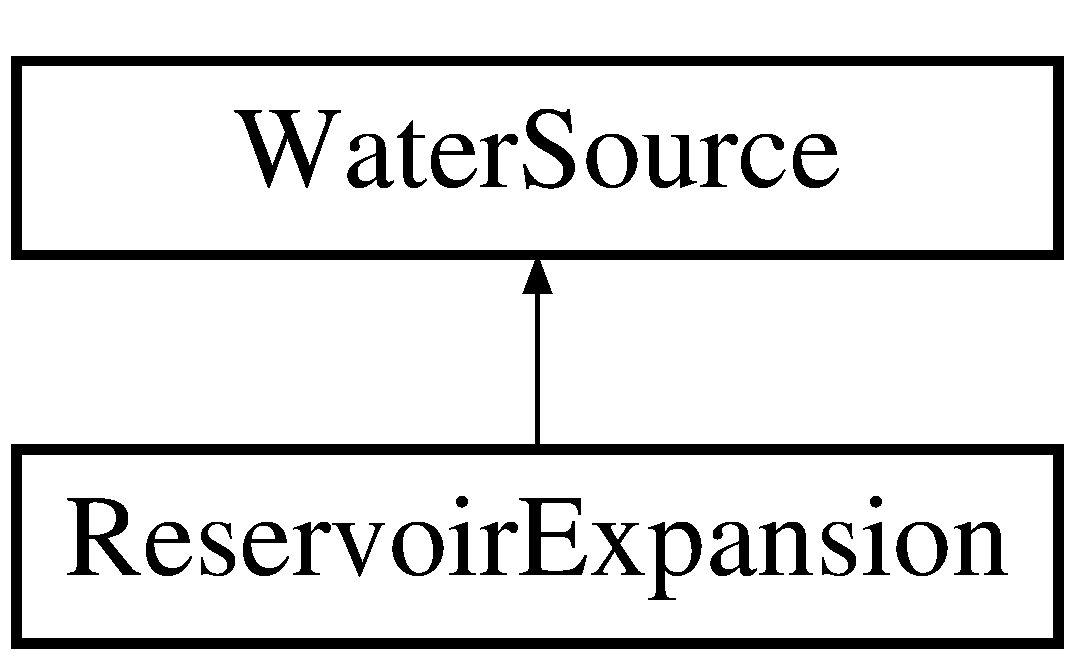
\includegraphics[height=2.000000cm]{classReservoirExpansion}
\end{center}
\end{figure}
\subsection*{Public Member Functions}
\begin{DoxyCompactItemize}
\item 
\mbox{\hyperlink{classReservoirExpansion_aa742cae4276e97847681dac4f828b5ae}{Reservoir\+Expansion}} (const char $\ast$\mbox{\hyperlink{classWaterSource_a846ea74c5b453d014f594d41fee8c765}{name}}, const int \mbox{\hyperlink{classWaterSource_a6eafe5dfefd317877d1244e8a7c6e742}{id}}, const unsigned int \mbox{\hyperlink{classReservoirExpansion_a56527196174404cfed20b863df2ab0ba}{parent\+\_\+reservoir\+\_\+\+ID}}, const double \mbox{\hyperlink{classWaterSource_a2ec257b415b248214a8bce7fc5267723}{capacity}}, const vector$<$ double $>$ \&construction\+\_\+time\+\_\+range, double permitting\+\_\+period, \mbox{\hyperlink{classBond}{Bond}} \&bond)
\begin{DoxyCompactList}\small\item\em Constructor for creating a \mbox{\hyperlink{classReservoirExpansion}{Reservoir\+Expansion}} object. \end{DoxyCompactList}\item 
\mbox{\hyperlink{classReservoirExpansion_abc10a6725f7fb85b7478fb6b0b79bd1e}{Reservoir\+Expansion}} (const \mbox{\hyperlink{classReservoirExpansion}{Reservoir\+Expansion}} \&reservoir\+\_\+expansion)
\begin{DoxyCompactList}\small\item\em Copy constructor for the \mbox{\hyperlink{classReservoirExpansion}{Reservoir\+Expansion}} class. \end{DoxyCompactList}\item 
\mbox{\hyperlink{classReservoirExpansion}{Reservoir\+Expansion}} \& \mbox{\hyperlink{classReservoirExpansion_a6c9607be0fc7ce624a19bc32fdff9222}{operator=}} (const \mbox{\hyperlink{classReservoirExpansion}{Reservoir\+Expansion}} \&reservoir\+\_\+expansion)
\begin{DoxyCompactList}\small\item\em Assignment operator for the \mbox{\hyperlink{classReservoirExpansion}{Reservoir\+Expansion}} class. \end{DoxyCompactList}\item 
void \mbox{\hyperlink{classReservoirExpansion_a18614050354dced5cc2747eeda0c2397}{apply\+Continuity}} (int week, double \mbox{\hyperlink{classWaterSource_a7a69b2e9b6030f1035e6cf44d2918ee5}{upstream\+\_\+source\+\_\+inflow}}, double wastewater\+\_\+discharge, vector$<$ double $>$ \&demand\+\_\+outflow) override
\begin{DoxyCompactList}\small\item\em Throws an error indicating that continuity cannot be applied to a reservoir expansion. \end{DoxyCompactList}\end{DoxyCompactItemize}
\subsection*{Public Attributes}
\begin{DoxyCompactItemize}
\item 
const unsigned int \mbox{\hyperlink{classReservoirExpansion_a56527196174404cfed20b863df2ab0ba}{parent\+\_\+reservoir\+\_\+\+ID}}
\begin{DoxyCompactList}\small\item\em The ID of the parent reservoir that is being expanded. \end{DoxyCompactList}\end{DoxyCompactItemize}
\subsection*{Additional Inherited Members}


\subsection{Constructor \& Destructor Documentation}
\mbox{\Hypertarget{classReservoirExpansion_aa742cae4276e97847681dac4f828b5ae}\label{classReservoirExpansion_aa742cae4276e97847681dac4f828b5ae}} 
\index{Reservoir\+Expansion@{Reservoir\+Expansion}!Reservoir\+Expansion@{Reservoir\+Expansion}}
\index{Reservoir\+Expansion@{Reservoir\+Expansion}!Reservoir\+Expansion@{Reservoir\+Expansion}}
\subsubsection{\texorpdfstring{Reservoir\+Expansion()}{ReservoirExpansion()}\hspace{0.1cm}{\footnotesize\ttfamily [1/2]}}
{\footnotesize\ttfamily Reservoir\+Expansion\+::\+Reservoir\+Expansion (\begin{DoxyParamCaption}\item[{const char $\ast$}]{name,  }\item[{const int}]{id,  }\item[{const unsigned int}]{parent\+\_\+reservoir\+\_\+\+ID,  }\item[{const double}]{capacity,  }\item[{const vector$<$ double $>$ \&}]{construction\+\_\+time\+\_\+range,  }\item[{double}]{permitting\+\_\+period,  }\item[{\mbox{\hyperlink{classBond}{Bond}} \&}]{bond }\end{DoxyParamCaption})}



Constructor for creating a \mbox{\hyperlink{classReservoirExpansion}{Reservoir\+Expansion}} object. 

This constructor initializes a {\ttfamily \mbox{\hyperlink{classReservoirExpansion}{Reservoir\+Expansion}}} object with the specified parameters and sets the parent reservoir ID. It also calls the constructor of the base class {\ttfamily \mbox{\hyperlink{classWaterSource}{Water\+Source}}} to initialize the shared attributes.


\begin{DoxyParams}{Parameters}
{\em name} & The name of the reservoir expansion. \\
\hline
{\em id} & The unique identifier for the reservoir expansion. \\
\hline
{\em parent\+\_\+reservoir\+\_\+\+ID} & The ID of the parent reservoir. \\
\hline
{\em capacity} & The capacity of the reservoir expansion. \\
\hline
{\em construction\+\_\+time\+\_\+range} & The time range for construction of the reservoir expansion. \\
\hline
{\em permitting\+\_\+period} & The permitting period for the reservoir expansion. \\
\hline
{\em bond} & A reference to the bond object associated with the reservoir expansion. \\
\hline
\end{DoxyParams}
\mbox{\Hypertarget{classReservoirExpansion_abc10a6725f7fb85b7478fb6b0b79bd1e}\label{classReservoirExpansion_abc10a6725f7fb85b7478fb6b0b79bd1e}} 
\index{Reservoir\+Expansion@{Reservoir\+Expansion}!Reservoir\+Expansion@{Reservoir\+Expansion}}
\index{Reservoir\+Expansion@{Reservoir\+Expansion}!Reservoir\+Expansion@{Reservoir\+Expansion}}
\subsubsection{\texorpdfstring{Reservoir\+Expansion()}{ReservoirExpansion()}\hspace{0.1cm}{\footnotesize\ttfamily [2/2]}}
{\footnotesize\ttfamily Reservoir\+Expansion\+::\+Reservoir\+Expansion (\begin{DoxyParamCaption}\item[{const \mbox{\hyperlink{classReservoirExpansion}{Reservoir\+Expansion}} \&}]{reservoir\+\_\+expansion }\end{DoxyParamCaption})}



Copy constructor for the \mbox{\hyperlink{classReservoirExpansion}{Reservoir\+Expansion}} class. 

This constructor creates a copy of an existing {\ttfamily \mbox{\hyperlink{classReservoirExpansion}{Reservoir\+Expansion}}} object by copying the values of its attributes, including calling the copy constructor of the base class {\ttfamily \mbox{\hyperlink{classWaterSource}{Water\+Source}}}.


\begin{DoxyParams}{Parameters}
{\em reservoir\+\_\+expansion} & The {\ttfamily \mbox{\hyperlink{classReservoirExpansion}{Reservoir\+Expansion}}} object to copy. \\
\hline
\end{DoxyParams}


\subsection{Member Function Documentation}
\mbox{\Hypertarget{classReservoirExpansion_a18614050354dced5cc2747eeda0c2397}\label{classReservoirExpansion_a18614050354dced5cc2747eeda0c2397}} 
\index{Reservoir\+Expansion@{Reservoir\+Expansion}!apply\+Continuity@{apply\+Continuity}}
\index{apply\+Continuity@{apply\+Continuity}!Reservoir\+Expansion@{Reservoir\+Expansion}}
\subsubsection{\texorpdfstring{apply\+Continuity()}{applyContinuity()}}
{\footnotesize\ttfamily void Reservoir\+Expansion\+::apply\+Continuity (\begin{DoxyParamCaption}\item[{int}]{week,  }\item[{double}]{upstream\+\_\+source\+\_\+inflow,  }\item[{double}]{wastewater\+\_\+discharge,  }\item[{vector$<$ double $>$ \&}]{demand\+\_\+outflow }\end{DoxyParamCaption})\hspace{0.3cm}{\ttfamily [override]}, {\ttfamily [virtual]}}



Throws an error indicating that continuity cannot be applied to a reservoir expansion. 

This function throws a {\ttfamily logic\+\_\+error} because a reservoir expansion only adds storage volume to the reservoir it is assigned to. Continuity calculations should be applied to the reservoir being expanded, not the expansion itself.


\begin{DoxyParams}{Parameters}
{\em week} & The week for which continuity would be applied. \\
\hline
{\em upstream\+\_\+source\+\_\+inflow} & The inflow from upstream sources (not used). \\
\hline
{\em wastewater\+\_\+discharge} & The inflow from wastewater discharge (not used). \\
\hline
{\em demand\+\_\+outflow} & A vector of demand outflows (not used).\\
\hline
\end{DoxyParams}

\begin{DoxyExceptions}{Exceptions}
{\em logic\+\_\+error} & This function always throws a {\ttfamily logic\+\_\+error} because continuity cannot be applied to a reservoir expansion. \\
\hline
\end{DoxyExceptions}


Implements \mbox{\hyperlink{classWaterSource_ac070445379fe706f65b977dade4f3fbc}{Water\+Source}}.

\mbox{\Hypertarget{classReservoirExpansion_a6c9607be0fc7ce624a19bc32fdff9222}\label{classReservoirExpansion_a6c9607be0fc7ce624a19bc32fdff9222}} 
\index{Reservoir\+Expansion@{Reservoir\+Expansion}!operator=@{operator=}}
\index{operator=@{operator=}!Reservoir\+Expansion@{Reservoir\+Expansion}}
\subsubsection{\texorpdfstring{operator=()}{operator=()}}
{\footnotesize\ttfamily \mbox{\hyperlink{classReservoirExpansion}{Reservoir\+Expansion}}\& Reservoir\+Expansion\+::operator= (\begin{DoxyParamCaption}\item[{const \mbox{\hyperlink{classReservoirExpansion}{Reservoir\+Expansion}} \&}]{reservoir\+\_\+expansion }\end{DoxyParamCaption})}



Assignment operator for the \mbox{\hyperlink{classReservoirExpansion}{Reservoir\+Expansion}} class. 

This operator assigns the values of one {\ttfamily \mbox{\hyperlink{classReservoirExpansion}{Reservoir\+Expansion}}} object to another.


\begin{DoxyParams}{Parameters}
{\em reservoir\+\_\+expansion} & The {\ttfamily \mbox{\hyperlink{classReservoirExpansion}{Reservoir\+Expansion}}} object to assign from.\\
\hline
\end{DoxyParams}
\begin{DoxyReturn}{Returns}
A reference to the current {\ttfamily \mbox{\hyperlink{classReservoirExpansion}{Reservoir\+Expansion}}} object after assignment. 
\end{DoxyReturn}


\subsection{Member Data Documentation}
\mbox{\Hypertarget{classReservoirExpansion_a56527196174404cfed20b863df2ab0ba}\label{classReservoirExpansion_a56527196174404cfed20b863df2ab0ba}} 
\index{Reservoir\+Expansion@{Reservoir\+Expansion}!parent\+\_\+reservoir\+\_\+\+ID@{parent\+\_\+reservoir\+\_\+\+ID}}
\index{parent\+\_\+reservoir\+\_\+\+ID@{parent\+\_\+reservoir\+\_\+\+ID}!Reservoir\+Expansion@{Reservoir\+Expansion}}
\subsubsection{\texorpdfstring{parent\+\_\+reservoir\+\_\+\+ID}{parent\_reservoir\_ID}}
{\footnotesize\ttfamily const unsigned int Reservoir\+Expansion\+::parent\+\_\+reservoir\+\_\+\+ID}



The ID of the parent reservoir that is being expanded. 



The documentation for this class was generated from the following file\+:\begin{DoxyCompactItemize}
\item 
/home/fs02/pmr82\+\_\+0001/lbl59/\+Water\+Paths-\/doc/src/\+System\+Components/\+Water\+Sources/\mbox{\hyperlink{ReservoirExpansion_8h}{Reservoir\+Expansion.\+h}}\end{DoxyCompactItemize}

\hypertarget{classSequentialJointTreatmentExpansion}{}\section{Sequential\+Joint\+Treatment\+Expansion Class Reference}
\label{classSequentialJointTreatmentExpansion}\index{Sequential\+Joint\+Treatment\+Expansion@{Sequential\+Joint\+Treatment\+Expansion}}


{\ttfamily \#include $<$Sequential\+Joint\+Treatment\+Expansion.\+h$>$}

Inheritance diagram for Sequential\+Joint\+Treatment\+Expansion\+:\begin{figure}[H]
\begin{center}
\leavevmode
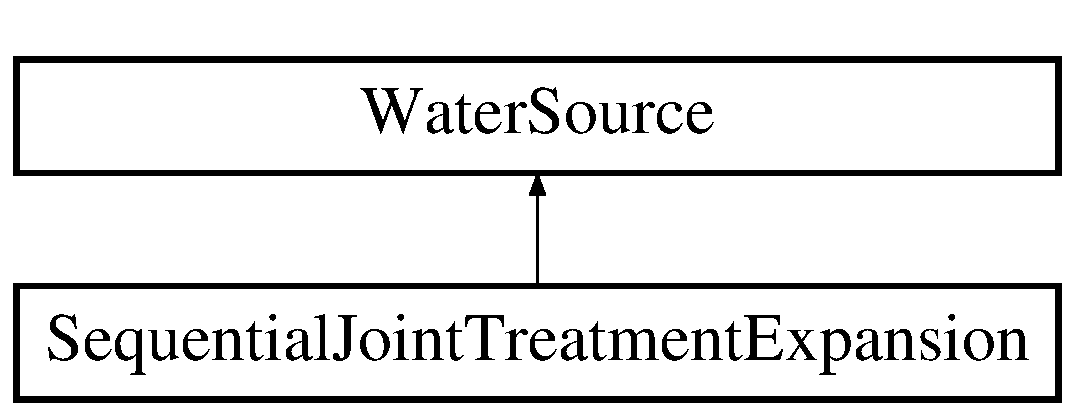
\includegraphics[height=2.000000cm]{classSequentialJointTreatmentExpansion}
\end{center}
\end{figure}
\subsection*{Public Member Functions}
\begin{DoxyCompactItemize}
\item 
\mbox{\hyperlink{classSequentialJointTreatmentExpansion_ad3ca28eaaa041be6ebbd0a4593d5c9ab}{Sequential\+Joint\+Treatment\+Expansion}} (const char $\ast$\mbox{\hyperlink{classWaterSource_a846ea74c5b453d014f594d41fee8c765}{name}}, const int \mbox{\hyperlink{classWaterSource_a6eafe5dfefd317877d1244e8a7c6e742}{id}}, const int \mbox{\hyperlink{classSequentialJointTreatmentExpansion_a43b9e27138606bbbf8e5ef0279232a0a}{parent\+\_\+reservoir\+\_\+\+ID}}, const int \mbox{\hyperlink{classSequentialJointTreatmentExpansion_adeaf6ba2bcfc4c024e332764144e3021}{expansion\+\_\+sequence\+\_\+id}}, vector$<$ int $>$ connected\+\_\+sources, vector$<$ double $>$ \&sequential\+\_\+treatment\+\_\+capacity, vector$<$ \mbox{\hyperlink{classBond}{Bond}} $\ast$$>$ \&\mbox{\hyperlink{classWaterSource_a413b094e11bdce62f4d82e5bb9e4706e}{bonds}}, const vector$<$ double $>$ \&construction\+\_\+time\+\_\+range, double permitting\+\_\+period)
\item 
\mbox{\hyperlink{classSequentialJointTreatmentExpansion_a677aa8de08ba7116216509b1a6d74b14}{Sequential\+Joint\+Treatment\+Expansion}} (const \mbox{\hyperlink{classSequentialJointTreatmentExpansion}{Sequential\+Joint\+Treatment\+Expansion}} \&joint\+\_\+water\+\_\+treatment\+\_\+plant)
\item 
\mbox{\hyperlink{classSequentialJointTreatmentExpansion_a77d4270fd89d172739fdede5b9e6c1e9}{$\sim$\+Sequential\+Joint\+Treatment\+Expansion}} () override
\item 
\mbox{\hyperlink{classSequentialJointTreatmentExpansion}{Sequential\+Joint\+Treatment\+Expansion}} \& \mbox{\hyperlink{classSequentialJointTreatmentExpansion_a53413658de78fecdb2e0d451a20eb82c}{operator=}} (const \mbox{\hyperlink{classSequentialJointTreatmentExpansion}{Sequential\+Joint\+Treatment\+Expansion}} \&joint\+\_\+water\+\_\+treatment\+\_\+plant)
\item 
void \mbox{\hyperlink{classSequentialJointTreatmentExpansion_a64fdd68fc68f6b1145291575c2116815}{apply\+Continuity}} (int week, double \mbox{\hyperlink{classWaterSource_a7a69b2e9b6030f1035e6cf44d2918ee5}{upstream\+\_\+source\+\_\+inflow}}, double wastewater\+\_\+discharge, vector$<$ double $>$ \&demand\+\_\+outflow) override
\item 
double \mbox{\hyperlink{classSequentialJointTreatmentExpansion_a06a2e9479bd639661cd8241e571c5711}{implement\+Treatment\+Capacity}} (int utility\+\_\+id)
\end{DoxyCompactItemize}
\subsection*{Public Attributes}
\begin{DoxyCompactItemize}
\item 
const int \mbox{\hyperlink{classSequentialJointTreatmentExpansion_adeaf6ba2bcfc4c024e332764144e3021}{expansion\+\_\+sequence\+\_\+id}}
\item 
const unsigned int \mbox{\hyperlink{classSequentialJointTreatmentExpansion_a43b9e27138606bbbf8e5ef0279232a0a}{parent\+\_\+reservoir\+\_\+\+ID}}
\end{DoxyCompactItemize}
\subsection*{Additional Inherited Members}


\subsection{Constructor \& Destructor Documentation}
\mbox{\Hypertarget{classSequentialJointTreatmentExpansion_ad3ca28eaaa041be6ebbd0a4593d5c9ab}\label{classSequentialJointTreatmentExpansion_ad3ca28eaaa041be6ebbd0a4593d5c9ab}} 
\index{Sequential\+Joint\+Treatment\+Expansion@{Sequential\+Joint\+Treatment\+Expansion}!Sequential\+Joint\+Treatment\+Expansion@{Sequential\+Joint\+Treatment\+Expansion}}
\index{Sequential\+Joint\+Treatment\+Expansion@{Sequential\+Joint\+Treatment\+Expansion}!Sequential\+Joint\+Treatment\+Expansion@{Sequential\+Joint\+Treatment\+Expansion}}
\subsubsection{\texorpdfstring{Sequential\+Joint\+Treatment\+Expansion()}{SequentialJointTreatmentExpansion()}\hspace{0.1cm}{\footnotesize\ttfamily [1/2]}}
{\footnotesize\ttfamily Sequential\+Joint\+Treatment\+Expansion\+::\+Sequential\+Joint\+Treatment\+Expansion (\begin{DoxyParamCaption}\item[{const char $\ast$}]{name,  }\item[{const int}]{id,  }\item[{const int}]{parent\+\_\+reservoir\+\_\+\+ID,  }\item[{const int}]{expansion\+\_\+sequence\+\_\+id,  }\item[{vector$<$ int $>$}]{connected\+\_\+sources,  }\item[{vector$<$ double $>$ \&}]{sequential\+\_\+treatment\+\_\+capacity,  }\item[{vector$<$ \mbox{\hyperlink{classBond}{Bond}} $\ast$$>$ \&}]{bonds,  }\item[{const vector$<$ double $>$ \&}]{construction\+\_\+time\+\_\+range,  }\item[{double}]{permitting\+\_\+period }\end{DoxyParamCaption})}


\begin{DoxyParams}{Parameters}
{\em name} & \\
\hline
{\em id} & \\
\hline
{\em parent\+\_\+reservoir\+\_\+\+ID} & \\
\hline
{\em expansion\+\_\+sequence\+\_\+id} & \\
\hline
{\em sequential\+\_\+treatment\+\_\+capacity} & \\
\hline
{\em bonds} & \\
\hline
{\em construction\+\_\+time\+\_\+range} & \\
\hline
{\em permitting\+\_\+period} & \\
\hline
\end{DoxyParams}
\mbox{\Hypertarget{classSequentialJointTreatmentExpansion_a677aa8de08ba7116216509b1a6d74b14}\label{classSequentialJointTreatmentExpansion_a677aa8de08ba7116216509b1a6d74b14}} 
\index{Sequential\+Joint\+Treatment\+Expansion@{Sequential\+Joint\+Treatment\+Expansion}!Sequential\+Joint\+Treatment\+Expansion@{Sequential\+Joint\+Treatment\+Expansion}}
\index{Sequential\+Joint\+Treatment\+Expansion@{Sequential\+Joint\+Treatment\+Expansion}!Sequential\+Joint\+Treatment\+Expansion@{Sequential\+Joint\+Treatment\+Expansion}}
\subsubsection{\texorpdfstring{Sequential\+Joint\+Treatment\+Expansion()}{SequentialJointTreatmentExpansion()}\hspace{0.1cm}{\footnotesize\ttfamily [2/2]}}
{\footnotesize\ttfamily Sequential\+Joint\+Treatment\+Expansion\+::\+Sequential\+Joint\+Treatment\+Expansion (\begin{DoxyParamCaption}\item[{const \mbox{\hyperlink{classSequentialJointTreatmentExpansion}{Sequential\+Joint\+Treatment\+Expansion}} \&}]{joint\+\_\+water\+\_\+treatment\+\_\+plant }\end{DoxyParamCaption})}

Copy constructor. 
\begin{DoxyParams}{Parameters}
{\em reservoir} & \\
\hline
\end{DoxyParams}
\mbox{\Hypertarget{classSequentialJointTreatmentExpansion_a77d4270fd89d172739fdede5b9e6c1e9}\label{classSequentialJointTreatmentExpansion_a77d4270fd89d172739fdede5b9e6c1e9}} 
\index{Sequential\+Joint\+Treatment\+Expansion@{Sequential\+Joint\+Treatment\+Expansion}!````~Sequential\+Joint\+Treatment\+Expansion@{$\sim$\+Sequential\+Joint\+Treatment\+Expansion}}
\index{````~Sequential\+Joint\+Treatment\+Expansion@{$\sim$\+Sequential\+Joint\+Treatment\+Expansion}!Sequential\+Joint\+Treatment\+Expansion@{Sequential\+Joint\+Treatment\+Expansion}}
\subsubsection{\texorpdfstring{$\sim$\+Sequential\+Joint\+Treatment\+Expansion()}{~SequentialJointTreatmentExpansion()}}
{\footnotesize\ttfamily Sequential\+Joint\+Treatment\+Expansion\+::$\sim$\+Sequential\+Joint\+Treatment\+Expansion (\begin{DoxyParamCaption}{ }\end{DoxyParamCaption})\hspace{0.3cm}{\ttfamily [override]}, {\ttfamily [default]}}



\subsection{Member Function Documentation}
\mbox{\Hypertarget{classSequentialJointTreatmentExpansion_a64fdd68fc68f6b1145291575c2116815}\label{classSequentialJointTreatmentExpansion_a64fdd68fc68f6b1145291575c2116815}} 
\index{Sequential\+Joint\+Treatment\+Expansion@{Sequential\+Joint\+Treatment\+Expansion}!apply\+Continuity@{apply\+Continuity}}
\index{apply\+Continuity@{apply\+Continuity}!Sequential\+Joint\+Treatment\+Expansion@{Sequential\+Joint\+Treatment\+Expansion}}
\subsubsection{\texorpdfstring{apply\+Continuity()}{applyContinuity()}}
{\footnotesize\ttfamily void Sequential\+Joint\+Treatment\+Expansion\+::apply\+Continuity (\begin{DoxyParamCaption}\item[{int}]{week,  }\item[{double}]{upstream\+\_\+source\+\_\+inflow,  }\item[{double}]{wastewater\+\_\+discharge,  }\item[{vector$<$ double $>$ \&}]{demand\+\_\+outflow }\end{DoxyParamCaption})\hspace{0.3cm}{\ttfamily [override]}, {\ttfamily [virtual]}}



Implements \mbox{\hyperlink{classWaterSource_ac070445379fe706f65b977dade4f3fbc}{Water\+Source}}.

\mbox{\Hypertarget{classSequentialJointTreatmentExpansion_a06a2e9479bd639661cd8241e571c5711}\label{classSequentialJointTreatmentExpansion_a06a2e9479bd639661cd8241e571c5711}} 
\index{Sequential\+Joint\+Treatment\+Expansion@{Sequential\+Joint\+Treatment\+Expansion}!implement\+Treatment\+Capacity@{implement\+Treatment\+Capacity}}
\index{implement\+Treatment\+Capacity@{implement\+Treatment\+Capacity}!Sequential\+Joint\+Treatment\+Expansion@{Sequential\+Joint\+Treatment\+Expansion}}
\subsubsection{\texorpdfstring{implement\+Treatment\+Capacity()}{implementTreatmentCapacity()}}
{\footnotesize\ttfamily double Sequential\+Joint\+Treatment\+Expansion\+::implement\+Treatment\+Capacity (\begin{DoxyParamCaption}\item[{int}]{utility\+\_\+id }\end{DoxyParamCaption})}

Returns the capacity to be installed for a given utility and deducts it from maximum planned expansion. 
\begin{DoxyParams}{Parameters}
{\em utility\+\_\+id} & \\
\hline
\end{DoxyParams}
\begin{DoxyReturn}{Returns}

\end{DoxyReturn}
\mbox{\Hypertarget{classSequentialJointTreatmentExpansion_a53413658de78fecdb2e0d451a20eb82c}\label{classSequentialJointTreatmentExpansion_a53413658de78fecdb2e0d451a20eb82c}} 
\index{Sequential\+Joint\+Treatment\+Expansion@{Sequential\+Joint\+Treatment\+Expansion}!operator=@{operator=}}
\index{operator=@{operator=}!Sequential\+Joint\+Treatment\+Expansion@{Sequential\+Joint\+Treatment\+Expansion}}
\subsubsection{\texorpdfstring{operator=()}{operator=()}}
{\footnotesize\ttfamily \mbox{\hyperlink{classSequentialJointTreatmentExpansion}{Sequential\+Joint\+Treatment\+Expansion}} \& Sequential\+Joint\+Treatment\+Expansion\+::operator= (\begin{DoxyParamCaption}\item[{const \mbox{\hyperlink{classSequentialJointTreatmentExpansion}{Sequential\+Joint\+Treatment\+Expansion}} \&}]{joint\+\_\+water\+\_\+treatment\+\_\+plant }\end{DoxyParamCaption})}

Copy assignment operator 
\begin{DoxyParams}{Parameters}
{\em reservoir} & \\
\hline
\end{DoxyParams}
\begin{DoxyReturn}{Returns}

\end{DoxyReturn}


\subsection{Member Data Documentation}
\mbox{\Hypertarget{classSequentialJointTreatmentExpansion_adeaf6ba2bcfc4c024e332764144e3021}\label{classSequentialJointTreatmentExpansion_adeaf6ba2bcfc4c024e332764144e3021}} 
\index{Sequential\+Joint\+Treatment\+Expansion@{Sequential\+Joint\+Treatment\+Expansion}!expansion\+\_\+sequence\+\_\+id@{expansion\+\_\+sequence\+\_\+id}}
\index{expansion\+\_\+sequence\+\_\+id@{expansion\+\_\+sequence\+\_\+id}!Sequential\+Joint\+Treatment\+Expansion@{Sequential\+Joint\+Treatment\+Expansion}}
\subsubsection{\texorpdfstring{expansion\+\_\+sequence\+\_\+id}{expansion\_sequence\_id}}
{\footnotesize\ttfamily const int Sequential\+Joint\+Treatment\+Expansion\+::expansion\+\_\+sequence\+\_\+id}

\mbox{\Hypertarget{classSequentialJointTreatmentExpansion_a43b9e27138606bbbf8e5ef0279232a0a}\label{classSequentialJointTreatmentExpansion_a43b9e27138606bbbf8e5ef0279232a0a}} 
\index{Sequential\+Joint\+Treatment\+Expansion@{Sequential\+Joint\+Treatment\+Expansion}!parent\+\_\+reservoir\+\_\+\+ID@{parent\+\_\+reservoir\+\_\+\+ID}}
\index{parent\+\_\+reservoir\+\_\+\+ID@{parent\+\_\+reservoir\+\_\+\+ID}!Sequential\+Joint\+Treatment\+Expansion@{Sequential\+Joint\+Treatment\+Expansion}}
\subsubsection{\texorpdfstring{parent\+\_\+reservoir\+\_\+\+ID}{parent\_reservoir\_ID}}
{\footnotesize\ttfamily const unsigned int Sequential\+Joint\+Treatment\+Expansion\+::parent\+\_\+reservoir\+\_\+\+ID}



The documentation for this class was generated from the following files\+:\begin{DoxyCompactItemize}
\item 
src/\+System\+Components/\+Water\+Sources/\mbox{\hyperlink{SequentialJointTreatmentExpansion_8h}{Sequential\+Joint\+Treatment\+Expansion.\+h}}\item 
src/\+System\+Components/\+Water\+Sources/\mbox{\hyperlink{SequentialJointTreatmentExpansion_8cpp}{Sequential\+Joint\+Treatment\+Expansion.\+cpp}}\end{DoxyCompactItemize}

\hypertarget{classSimulation}{}\section{Simulation Class Reference}
\label{classSimulation}\index{Simulation@{Simulation}}


{\ttfamily \#include $<$Simulation.\+h$>$}

\subsection*{Public Member Functions}
\begin{DoxyCompactItemize}
\item 
\mbox{\hyperlink{classSimulation_ac9b9db9c3de5f9ff33f6ea89e2435c87}{Simulation}} (vector$<$ \mbox{\hyperlink{classWaterSource}{Water\+Source}} $\ast$$>$ \&water\+\_\+sources, \mbox{\hyperlink{classGraph}{Graph}} \&water\+\_\+sources\+\_\+graph, const vector$<$ vector$<$ int $>$$>$ \&water\+\_\+sources\+\_\+to\+\_\+utilities, vector$<$ \mbox{\hyperlink{classUtility}{Utility}} $\ast$$>$ \&utilities, const vector$<$ \mbox{\hyperlink{classDroughtMitigationPolicy}{Drought\+Mitigation\+Policy}} $\ast$$>$ \&drought\+\_\+mitigation\+\_\+policies, vector$<$ \mbox{\hyperlink{classMinEnvFlowControl}{Min\+Env\+Flow\+Control}} $\ast$$>$ \&min\+\_\+env\+\_\+flow\+\_\+controls, vector$<$ vector$<$ double $>$$>$ \&utilities\+\_\+rdm, vector$<$ vector$<$ double $>$$>$ \&water\+\_\+sources\+\_\+rdm, vector$<$ vector$<$ double $>$$>$ \&policies\+\_\+rdm, const unsigned long total\+\_\+simulation\+\_\+time, vector$<$ unsigned long $>$ \&realizations\+\_\+to\+\_\+run)
\item 
\mbox{\hyperlink{classSimulation_aa225c1836ebd788eb0f35c8cd53f0533}{Simulation}} (vector$<$ \mbox{\hyperlink{classWaterSource}{Water\+Source}} $\ast$$>$ \&water\+\_\+sources, \mbox{\hyperlink{classGraph}{Graph}} \&water\+\_\+sources\+\_\+graph, const vector$<$ vector$<$ int $>$$>$ \&water\+\_\+sources\+\_\+to\+\_\+utilities, vector$<$ \mbox{\hyperlink{classUtility}{Utility}} $\ast$$>$ \&utilities, const vector$<$ \mbox{\hyperlink{classDroughtMitigationPolicy}{Drought\+Mitigation\+Policy}} $\ast$$>$ \&drought\+\_\+mitigation\+\_\+policies, vector$<$ \mbox{\hyperlink{classMinEnvFlowControl}{Min\+Env\+Flow\+Control}} $\ast$$>$ \&min\+\_\+env\+\_\+flow\+\_\+controls, vector$<$ vector$<$ double $>$$>$ \&utilities\+\_\+rdm, vector$<$ vector$<$ double $>$$>$ \&water\+\_\+sources\+\_\+rdm, vector$<$ vector$<$ double $>$$>$ \&policies\+\_\+rdm, const unsigned long total\+\_\+simulation\+\_\+time, vector$<$ unsigned long $>$ \&realizations\+\_\+to\+\_\+run, vector$<$ vector$<$ \mbox{\hyperlink{classMatrix2D}{Matrix2D}}$<$ double $>$$>$$>$ \&precomputed\+\_\+rof\+\_\+tables, vector$<$ vector$<$ double $>$$>$ \&table\+\_\+storage\+\_\+shift, string \&rof\+\_\+tables\+\_\+folder)
\item 
\mbox{\hyperlink{classSimulation_a68f43435cf8308d5415cdfcdb84e1fac}{Simulation}} (vector$<$ \mbox{\hyperlink{classWaterSource}{Water\+Source}} $\ast$$>$ \&water\+\_\+sources, \mbox{\hyperlink{classGraph}{Graph}} \&water\+\_\+sources\+\_\+graph, const vector$<$ vector$<$ int $>$$>$ \&water\+\_\+sources\+\_\+to\+\_\+utilities, vector$<$ \mbox{\hyperlink{classUtility}{Utility}} $\ast$$>$ \&utilities, const vector$<$ \mbox{\hyperlink{classDroughtMitigationPolicy}{Drought\+Mitigation\+Policy}} $\ast$$>$ \&drought\+\_\+mitigation\+\_\+policies, vector$<$ \mbox{\hyperlink{classMinEnvFlowControl}{Min\+Env\+Flow\+Control}} $\ast$$>$ \&min\+\_\+env\+\_\+flow\+\_\+controls, vector$<$ vector$<$ double $>$$>$ \&utilities\+\_\+rdm, vector$<$ vector$<$ double $>$$>$ \&water\+\_\+sources\+\_\+rdm, vector$<$ vector$<$ double $>$$>$ \&policies\+\_\+rdm, const unsigned long total\+\_\+simulation\+\_\+time, vector$<$ unsigned long $>$ \&realizations\+\_\+to\+\_\+run, string \&rof\+\_\+tables\+\_\+folder)
\item 
\mbox{\hyperlink{classSimulation}{Simulation}} \& \mbox{\hyperlink{classSimulation_aa9ad48555e93d646d68c0df7a87e2356}{operator=}} (const \mbox{\hyperlink{classSimulation}{Simulation}} \&simulation)
\item 
virtual \mbox{\hyperlink{classSimulation_a80fad3f57dfaf195a36f7bc49bc88279}{$\sim$\+Simulation}} ()
\item 
\mbox{\hyperlink{classMasterDataCollector}{Master\+Data\+Collector}} $\ast$ \mbox{\hyperlink{classSimulation_acfd5f3442b2e6c59eeed6a7b2fabb0f6}{run\+Full\+Simulation}} (unsigned long n\+\_\+threads, double $\ast$vars)
\item 
void \mbox{\hyperlink{classSimulation_ac9ff965191f13b1ce044344fd1e5d0ac}{setup\+Simulation}} (vector$<$ \mbox{\hyperlink{classWaterSource}{Water\+Source}} $\ast$$>$ \&water\+\_\+sources, \mbox{\hyperlink{classGraph}{Graph}} \&water\+\_\+sources\+\_\+graph, const vector$<$ vector$<$ int $>$$>$ \&water\+\_\+sources\+\_\+to\+\_\+utilities, vector$<$ \mbox{\hyperlink{classUtility}{Utility}} $\ast$$>$ \&utilities, const vector$<$ \mbox{\hyperlink{classDroughtMitigationPolicy}{Drought\+Mitigation\+Policy}} $\ast$$>$ \&drought\+\_\+mitigation\+\_\+policies, vector$<$ \mbox{\hyperlink{classMinEnvFlowControl}{Min\+Env\+Flow\+Control}} $\ast$$>$ \&min\+\_\+env\+\_\+flow\+\_\+controls, vector$<$ vector$<$ double $>$$>$ \&utilities\+\_\+rdm, vector$<$ vector$<$ double $>$$>$ \&water\+\_\+sources\+\_\+rdm, vector$<$ vector$<$ double $>$$>$ \&policies\+\_\+rdm, vector$<$ unsigned long $>$ \&realizations\+\_\+to\+\_\+run)
\item 
void \mbox{\hyperlink{classSimulation_aa2e2863a0038345c46dd827b97008347}{create\+Continuity\+Models}} (unsigned long realization, \mbox{\hyperlink{classContinuityModelRealization}{Continuity\+Model\+Realization}} $\ast$\&realization\+\_\+model, \mbox{\hyperlink{classContinuityModelROF}{Continuity\+Model\+R\+OF}} $\ast$\&rof\+\_\+model)
\end{DoxyCompactItemize}


\subsection{Constructor \& Destructor Documentation}
\mbox{\Hypertarget{classSimulation_ac9b9db9c3de5f9ff33f6ea89e2435c87}\label{classSimulation_ac9b9db9c3de5f9ff33f6ea89e2435c87}} 
\index{Simulation@{Simulation}!Simulation@{Simulation}}
\index{Simulation@{Simulation}!Simulation@{Simulation}}
\subsubsection{\texorpdfstring{Simulation()}{Simulation()}\hspace{0.1cm}{\footnotesize\ttfamily [1/3]}}
{\footnotesize\ttfamily Simulation\+::\+Simulation (\begin{DoxyParamCaption}\item[{vector$<$ \mbox{\hyperlink{classWaterSource}{Water\+Source}} $\ast$$>$ \&}]{water\+\_\+sources,  }\item[{\mbox{\hyperlink{classGraph}{Graph}} \&}]{water\+\_\+sources\+\_\+graph,  }\item[{const vector$<$ vector$<$ int $>$$>$ \&}]{water\+\_\+sources\+\_\+to\+\_\+utilities,  }\item[{vector$<$ \mbox{\hyperlink{classUtility}{Utility}} $\ast$$>$ \&}]{utilities,  }\item[{const vector$<$ \mbox{\hyperlink{classDroughtMitigationPolicy}{Drought\+Mitigation\+Policy}} $\ast$$>$ \&}]{drought\+\_\+mitigation\+\_\+policies,  }\item[{vector$<$ \mbox{\hyperlink{classMinEnvFlowControl}{Min\+Env\+Flow\+Control}} $\ast$$>$ \&}]{min\+\_\+env\+\_\+flow\+\_\+controls,  }\item[{vector$<$ vector$<$ double $>$$>$ \&}]{utilities\+\_\+rdm,  }\item[{vector$<$ vector$<$ double $>$$>$ \&}]{water\+\_\+sources\+\_\+rdm,  }\item[{vector$<$ vector$<$ double $>$$>$ \&}]{policies\+\_\+rdm,  }\item[{const unsigned long}]{total\+\_\+simulation\+\_\+time,  }\item[{vector$<$ unsigned long $>$ \&}]{realizations\+\_\+to\+\_\+run }\end{DoxyParamCaption})}

\mbox{\Hypertarget{classSimulation_aa225c1836ebd788eb0f35c8cd53f0533}\label{classSimulation_aa225c1836ebd788eb0f35c8cd53f0533}} 
\index{Simulation@{Simulation}!Simulation@{Simulation}}
\index{Simulation@{Simulation}!Simulation@{Simulation}}
\subsubsection{\texorpdfstring{Simulation()}{Simulation()}\hspace{0.1cm}{\footnotesize\ttfamily [2/3]}}
{\footnotesize\ttfamily Simulation\+::\+Simulation (\begin{DoxyParamCaption}\item[{vector$<$ \mbox{\hyperlink{classWaterSource}{Water\+Source}} $\ast$$>$ \&}]{water\+\_\+sources,  }\item[{\mbox{\hyperlink{classGraph}{Graph}} \&}]{water\+\_\+sources\+\_\+graph,  }\item[{const vector$<$ vector$<$ int $>$$>$ \&}]{water\+\_\+sources\+\_\+to\+\_\+utilities,  }\item[{vector$<$ \mbox{\hyperlink{classUtility}{Utility}} $\ast$$>$ \&}]{utilities,  }\item[{const vector$<$ \mbox{\hyperlink{classDroughtMitigationPolicy}{Drought\+Mitigation\+Policy}} $\ast$$>$ \&}]{drought\+\_\+mitigation\+\_\+policies,  }\item[{vector$<$ \mbox{\hyperlink{classMinEnvFlowControl}{Min\+Env\+Flow\+Control}} $\ast$$>$ \&}]{min\+\_\+env\+\_\+flow\+\_\+controls,  }\item[{vector$<$ vector$<$ double $>$$>$ \&}]{utilities\+\_\+rdm,  }\item[{vector$<$ vector$<$ double $>$$>$ \&}]{water\+\_\+sources\+\_\+rdm,  }\item[{vector$<$ vector$<$ double $>$$>$ \&}]{policies\+\_\+rdm,  }\item[{const unsigned long}]{total\+\_\+simulation\+\_\+time,  }\item[{vector$<$ unsigned long $>$ \&}]{realizations\+\_\+to\+\_\+run,  }\item[{vector$<$ vector$<$ \mbox{\hyperlink{classMatrix2D}{Matrix2D}}$<$ double $>$$>$$>$ \&}]{precomputed\+\_\+rof\+\_\+tables,  }\item[{vector$<$ vector$<$ double $>$$>$ \&}]{table\+\_\+storage\+\_\+shift,  }\item[{string \&}]{rof\+\_\+tables\+\_\+folder }\end{DoxyParamCaption})}

\mbox{\Hypertarget{classSimulation_a68f43435cf8308d5415cdfcdb84e1fac}\label{classSimulation_a68f43435cf8308d5415cdfcdb84e1fac}} 
\index{Simulation@{Simulation}!Simulation@{Simulation}}
\index{Simulation@{Simulation}!Simulation@{Simulation}}
\subsubsection{\texorpdfstring{Simulation()}{Simulation()}\hspace{0.1cm}{\footnotesize\ttfamily [3/3]}}
{\footnotesize\ttfamily Simulation\+::\+Simulation (\begin{DoxyParamCaption}\item[{vector$<$ \mbox{\hyperlink{classWaterSource}{Water\+Source}} $\ast$$>$ \&}]{water\+\_\+sources,  }\item[{\mbox{\hyperlink{classGraph}{Graph}} \&}]{water\+\_\+sources\+\_\+graph,  }\item[{const vector$<$ vector$<$ int $>$$>$ \&}]{water\+\_\+sources\+\_\+to\+\_\+utilities,  }\item[{vector$<$ \mbox{\hyperlink{classUtility}{Utility}} $\ast$$>$ \&}]{utilities,  }\item[{const vector$<$ \mbox{\hyperlink{classDroughtMitigationPolicy}{Drought\+Mitigation\+Policy}} $\ast$$>$ \&}]{drought\+\_\+mitigation\+\_\+policies,  }\item[{vector$<$ \mbox{\hyperlink{classMinEnvFlowControl}{Min\+Env\+Flow\+Control}} $\ast$$>$ \&}]{min\+\_\+env\+\_\+flow\+\_\+controls,  }\item[{vector$<$ vector$<$ double $>$$>$ \&}]{utilities\+\_\+rdm,  }\item[{vector$<$ vector$<$ double $>$$>$ \&}]{water\+\_\+sources\+\_\+rdm,  }\item[{vector$<$ vector$<$ double $>$$>$ \&}]{policies\+\_\+rdm,  }\item[{const unsigned long}]{total\+\_\+simulation\+\_\+time,  }\item[{vector$<$ unsigned long $>$ \&}]{realizations\+\_\+to\+\_\+run,  }\item[{string \&}]{rof\+\_\+tables\+\_\+folder }\end{DoxyParamCaption})}

\mbox{\Hypertarget{classSimulation_a80fad3f57dfaf195a36f7bc49bc88279}\label{classSimulation_a80fad3f57dfaf195a36f7bc49bc88279}} 
\index{Simulation@{Simulation}!````~Simulation@{$\sim$\+Simulation}}
\index{````~Simulation@{$\sim$\+Simulation}!Simulation@{Simulation}}
\subsubsection{\texorpdfstring{$\sim$\+Simulation()}{~Simulation()}}
{\footnotesize\ttfamily Simulation\+::$\sim$\+Simulation (\begin{DoxyParamCaption}{ }\end{DoxyParamCaption})\hspace{0.3cm}{\ttfamily [virtual]}, {\ttfamily [default]}}



\subsection{Member Function Documentation}
\mbox{\Hypertarget{classSimulation_aa2e2863a0038345c46dd827b97008347}\label{classSimulation_aa2e2863a0038345c46dd827b97008347}} 
\index{Simulation@{Simulation}!create\+Continuity\+Models@{create\+Continuity\+Models}}
\index{create\+Continuity\+Models@{create\+Continuity\+Models}!Simulation@{Simulation}}
\subsubsection{\texorpdfstring{create\+Continuity\+Models()}{createContinuityModels()}}
{\footnotesize\ttfamily void Simulation\+::create\+Continuity\+Models (\begin{DoxyParamCaption}\item[{unsigned long}]{realization,  }\item[{\mbox{\hyperlink{classContinuityModelRealization}{Continuity\+Model\+Realization}} $\ast$\&}]{realization\+\_\+model,  }\item[{\mbox{\hyperlink{classContinuityModelROF}{Continuity\+Model\+R\+OF}} $\ast$\&}]{rof\+\_\+model }\end{DoxyParamCaption})}

\mbox{\Hypertarget{classSimulation_aa9ad48555e93d646d68c0df7a87e2356}\label{classSimulation_aa9ad48555e93d646d68c0df7a87e2356}} 
\index{Simulation@{Simulation}!operator=@{operator=}}
\index{operator=@{operator=}!Simulation@{Simulation}}
\subsubsection{\texorpdfstring{operator=()}{operator=()}}
{\footnotesize\ttfamily \mbox{\hyperlink{classSimulation}{Simulation}} \& Simulation\+::operator= (\begin{DoxyParamCaption}\item[{const \mbox{\hyperlink{classSimulation}{Simulation}} \&}]{simulation }\end{DoxyParamCaption})}

Assignment constructor 
\begin{DoxyParams}{Parameters}
{\em simulation} & \\
\hline
\end{DoxyParams}
\begin{DoxyReturn}{Returns}

\end{DoxyReturn}
\begin{DoxyRefDesc}{Todo}
\item[\mbox{\hyperlink{todo__todo000007}{Todo}}]implement assignment constructor. \end{DoxyRefDesc}
\mbox{\Hypertarget{classSimulation_acfd5f3442b2e6c59eeed6a7b2fabb0f6}\label{classSimulation_acfd5f3442b2e6c59eeed6a7b2fabb0f6}} 
\index{Simulation@{Simulation}!run\+Full\+Simulation@{run\+Full\+Simulation}}
\index{run\+Full\+Simulation@{run\+Full\+Simulation}!Simulation@{Simulation}}
\subsubsection{\texorpdfstring{run\+Full\+Simulation()}{runFullSimulation()}}
{\footnotesize\ttfamily \mbox{\hyperlink{classMasterDataCollector}{Master\+Data\+Collector}} $\ast$ Simulation\+::run\+Full\+Simulation (\begin{DoxyParamCaption}\item[{unsigned long}]{n\+\_\+threads,  }\item[{double $\ast$}]{vars }\end{DoxyParamCaption})}

\mbox{\Hypertarget{classSimulation_ac9ff965191f13b1ce044344fd1e5d0ac}\label{classSimulation_ac9ff965191f13b1ce044344fd1e5d0ac}} 
\index{Simulation@{Simulation}!setup\+Simulation@{setup\+Simulation}}
\index{setup\+Simulation@{setup\+Simulation}!Simulation@{Simulation}}
\subsubsection{\texorpdfstring{setup\+Simulation()}{setupSimulation()}}
{\footnotesize\ttfamily void Simulation\+::setup\+Simulation (\begin{DoxyParamCaption}\item[{vector$<$ \mbox{\hyperlink{classWaterSource}{Water\+Source}} $\ast$$>$ \&}]{water\+\_\+sources,  }\item[{\mbox{\hyperlink{classGraph}{Graph}} \&}]{water\+\_\+sources\+\_\+graph,  }\item[{const vector$<$ vector$<$ int $>$$>$ \&}]{water\+\_\+sources\+\_\+to\+\_\+utilities,  }\item[{vector$<$ \mbox{\hyperlink{classUtility}{Utility}} $\ast$$>$ \&}]{utilities,  }\item[{const vector$<$ \mbox{\hyperlink{classDroughtMitigationPolicy}{Drought\+Mitigation\+Policy}} $\ast$$>$ \&}]{drought\+\_\+mitigation\+\_\+policies,  }\item[{vector$<$ \mbox{\hyperlink{classMinEnvFlowControl}{Min\+Env\+Flow\+Control}} $\ast$$>$ \&}]{min\+\_\+env\+\_\+flow\+\_\+controls,  }\item[{vector$<$ vector$<$ double $>$$>$ \&}]{utilities\+\_\+rdm,  }\item[{vector$<$ vector$<$ double $>$$>$ \&}]{water\+\_\+sources\+\_\+rdm,  }\item[{vector$<$ vector$<$ double $>$$>$ \&}]{policies\+\_\+rdm,  }\item[{vector$<$ unsigned long $>$ \&}]{realizations\+\_\+to\+\_\+run }\end{DoxyParamCaption})}



The documentation for this class was generated from the following files\+:\begin{DoxyCompactItemize}
\item 
src/\+Simulation/\mbox{\hyperlink{Simulation_8h}{Simulation.\+h}}\item 
src/\+Simulation/\mbox{\hyperlink{Simulation_8cpp}{Simulation.\+cpp}}\end{DoxyCompactItemize}

\hypertarget{classTriangle}{}\section{Triangle Class Reference}
\label{classTriangle}\index{Triangle@{Triangle}}


{\ttfamily \#include $<$Triangle.\+h$>$}

Inheritance diagram for Triangle\+:\begin{figure}[H]
\begin{center}
\leavevmode
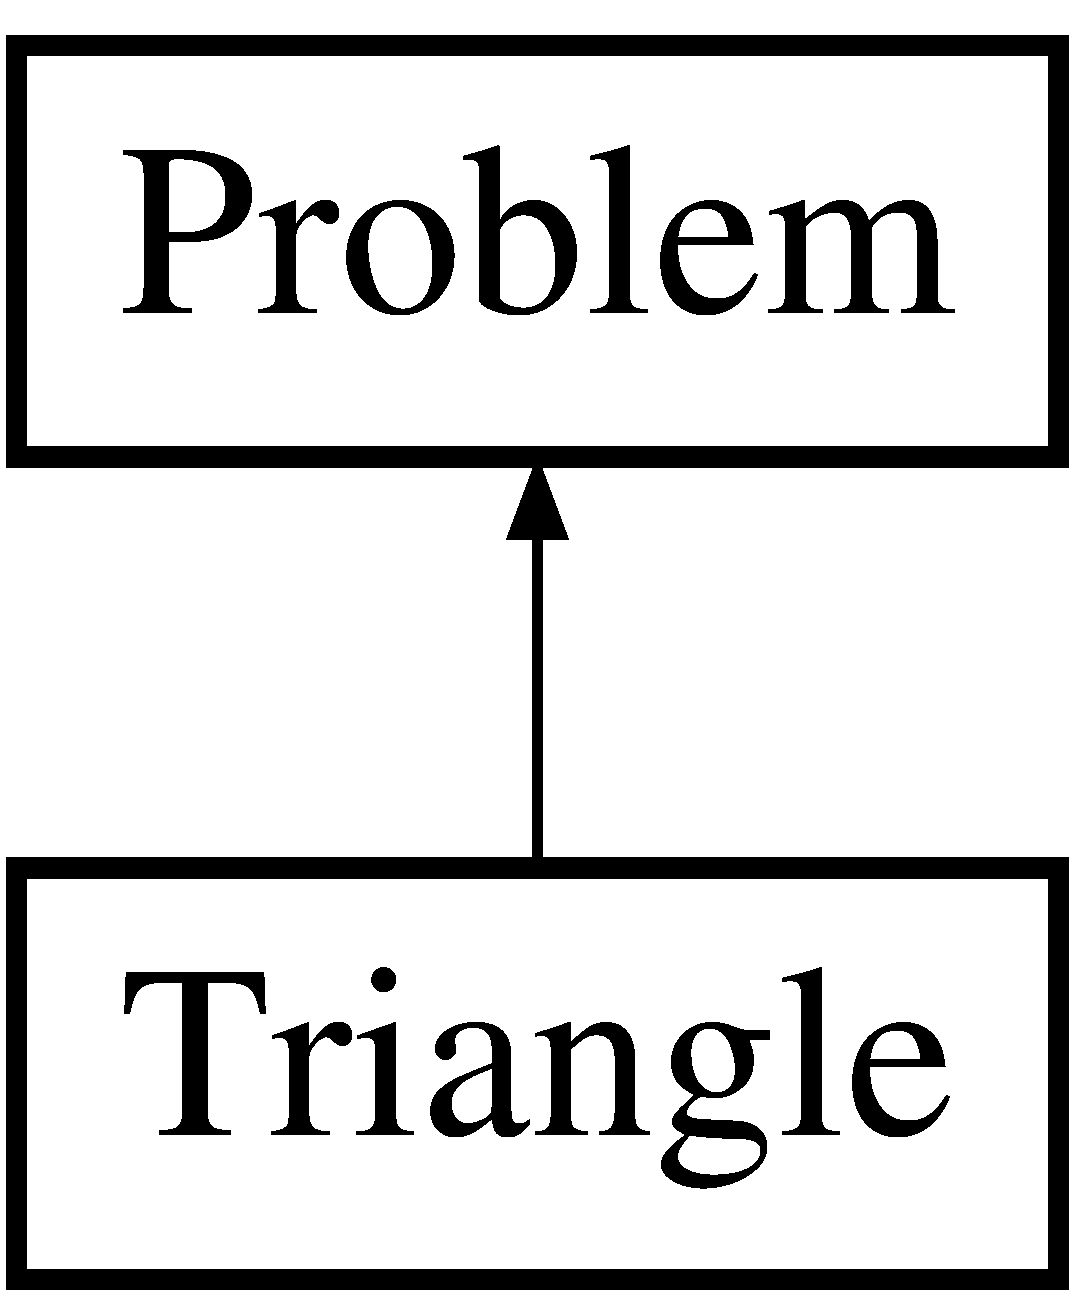
\includegraphics[height=2.000000cm]{classTriangle}
\end{center}
\end{figure}
\subsection*{Public Member Functions}
\begin{DoxyCompactItemize}
\item 
\mbox{\hyperlink{classTriangle_a24833bad242ddc3f671b36678dff5738_a24833bad242ddc3f671b36678dff5738}{Triangle}} (unsigned long \mbox{\hyperlink{classProblem_ac7513bb0ecdfa4bbb7d2ada3595d71ec_ac7513bb0ecdfa4bbb7d2ada3595d71ec}{n\+\_\+weeks}}, int import\+\_\+export\+\_\+rof\+\_\+table)
\item 
\mbox{\hyperlink{classTriangle_a5199760a17454f4dc94c855a57e3a152_a5199760a17454f4dc94c855a57e3a152}{$\sim$\+Triangle}} ()
\item 
int \mbox{\hyperlink{classTriangle_a9e95039d098fd61cce1a830b85ed7004_a9e95039d098fd61cce1a830b85ed7004}{function\+Evaluation}} (double $\ast$vars, double $\ast$objs, double $\ast$consts) override
\item 
int \mbox{\hyperlink{classTriangle_a816ff476231f6bd575c82978706f4b9a_a816ff476231f6bd575c82978706f4b9a}{simulation\+Exception\+Hander}} (const std\+::exception \&e, \mbox{\hyperlink{classSimulation}{Simulation}} $\ast$s, double $\ast$objs, const double $\ast$vars)
\item 
void \mbox{\hyperlink{classTriangle_a045e3263a62a8a628fe5645f0323b7e4_a045e3263a62a8a628fe5645f0323b7e4}{read\+Input\+Data}} ()
\end{DoxyCompactItemize}
\subsection*{Private Attributes}
\begin{DoxyCompactItemize}
\item 
const int \mbox{\hyperlink{classTriangle_a27fd697e6e14227b71a617ddbcec9653_a27fd697e6e14227b71a617ddbcec9653}{n\+\_\+utilities}} = 4
\item 
vector$<$ vector$<$ double $>$ $>$ \mbox{\hyperlink{classTriangle_a20fe79b08b5b0db16b3154d4d9a9b5eb_a20fe79b08b5b0db16b3154d4d9a9b5eb}{streamflows\+\_\+durham}}
\item 
vector$<$ vector$<$ double $>$ $>$ \mbox{\hyperlink{classTriangle_a1d93dad189b3fb422f5404f75a08b6f7_a1d93dad189b3fb422f5404f75a08b6f7}{streamflows\+\_\+flat}}
\item 
vector$<$ vector$<$ double $>$ $>$ \mbox{\hyperlink{classTriangle_a6fc8ddba9b9c2afea0ff19ac21343807_a6fc8ddba9b9c2afea0ff19ac21343807}{streamflows\+\_\+swift}}
\item 
vector$<$ vector$<$ double $>$ $>$ \mbox{\hyperlink{classTriangle_a776794a53c778e47ebe0f8a6b49cd740_a776794a53c778e47ebe0f8a6b49cd740}{streamflows\+\_\+llr}}
\item 
vector$<$ vector$<$ double $>$ $>$ \mbox{\hyperlink{classTriangle_a8c97075d74abc5e38084934fb213fe2a_a8c97075d74abc5e38084934fb213fe2a}{streamflows\+\_\+crabtree}}
\item 
vector$<$ vector$<$ double $>$ $>$ \mbox{\hyperlink{classTriangle_a936a703fc9bb94bce59bb0cbec005115_a936a703fc9bb94bce59bb0cbec005115}{streamflows\+\_\+phils}}
\item 
vector$<$ vector$<$ double $>$ $>$ \mbox{\hyperlink{classTriangle_a0a20ad805c77f2af96433b17eb3cc733_a0a20ad805c77f2af96433b17eb3cc733}{streamflows\+\_\+cane}}
\item 
vector$<$ vector$<$ double $>$ $>$ \mbox{\hyperlink{classTriangle_a3426e30cdc767333d491895438bdb00f_a3426e30cdc767333d491895438bdb00f}{streamflows\+\_\+morgan}}
\item 
vector$<$ vector$<$ double $>$ $>$ \mbox{\hyperlink{classTriangle_a2303d7ba019fa2c88ad9bcf4968b9522_a2303d7ba019fa2c88ad9bcf4968b9522}{streamflows\+\_\+haw}}
\item 
vector$<$ vector$<$ double $>$ $>$ \mbox{\hyperlink{classTriangle_a2c59e6b06ce2824ac697ca97c2423060_a2c59e6b06ce2824ac697ca97c2423060}{streamflows\+\_\+clayton}}
\item 
vector$<$ vector$<$ double $>$ $>$ \mbox{\hyperlink{classTriangle_ac69585cb9a4f8a477f030a3d66cea92f_ac69585cb9a4f8a477f030a3d66cea92f}{streamflows\+\_\+lillington}}
\item 
vector$<$ vector$<$ double $>$ $>$ \mbox{\hyperlink{classTriangle_a64dfcb5c1225f772fdadee71f776bc6a_a64dfcb5c1225f772fdadee71f776bc6a}{demand\+\_\+cary}}
\item 
vector$<$ vector$<$ double $>$ $>$ \mbox{\hyperlink{classTriangle_a0e82969571c5cdb51e98fe4b74a89597_a0e82969571c5cdb51e98fe4b74a89597}{demand\+\_\+durham}}
\item 
vector$<$ vector$<$ double $>$ $>$ \mbox{\hyperlink{classTriangle_a94d23326283d34b4000ac9c1ab6e848f_a94d23326283d34b4000ac9c1ab6e848f}{demand\+\_\+raleigh}}
\item 
vector$<$ vector$<$ double $>$ $>$ \mbox{\hyperlink{classTriangle_a3a3e2438a3c125a53d08101dc0ba82ac_a3a3e2438a3c125a53d08101dc0ba82ac}{demand\+\_\+owasa}}
\item 
vector$<$ vector$<$ double $>$ $>$ \mbox{\hyperlink{classTriangle_a11dd71d21edee3cf466d30117e378fb9_a11dd71d21edee3cf466d30117e378fb9}{evap\+\_\+durham}}
\item 
vector$<$ vector$<$ double $>$ $>$ \mbox{\hyperlink{classTriangle_a4ad865bba9e2b65233aa453ea95d1950_a4ad865bba9e2b65233aa453ea95d1950}{evap\+\_\+falls\+\_\+lake}}
\item 
vector$<$ vector$<$ double $>$ $>$ \mbox{\hyperlink{classTriangle_a9b1fbfcfe6230372f486382bd3b47717_a9b1fbfcfe6230372f486382bd3b47717}{evap\+\_\+owasa}}
\item 
vector$<$ vector$<$ double $>$ $>$ \mbox{\hyperlink{classTriangle_a48c51eabed2ace852d31b1df2e98f8d4_a48c51eabed2ace852d31b1df2e98f8d4}{evap\+\_\+little\+\_\+river}}
\item 
vector$<$ vector$<$ double $>$ $>$ \mbox{\hyperlink{classTriangle_a03a6df04c98f4a9030de3da381155cd8_a03a6df04c98f4a9030de3da381155cd8}{evap\+\_\+wheeler\+\_\+benson}}
\item 
vector$<$ vector$<$ double $>$ $>$ \mbox{\hyperlink{classTriangle_aa340181943eedb577bf81215e34701f5_aa340181943eedb577bf81215e34701f5}{evap\+\_\+jordan\+\_\+lake}}
\item 
vector$<$ vector$<$ double $>$ $>$ \mbox{\hyperlink{classTriangle_ac1aeb61eae9f469b139c38d688235724_ac1aeb61eae9f469b139c38d688235724}{demand\+\_\+to\+\_\+wastewater\+\_\+fraction\+\_\+owasa\+\_\+raleigh}}
\item 
vector$<$ vector$<$ double $>$ $>$ \mbox{\hyperlink{classTriangle_a69d6615c9468c9637a2ce0ea52e23930_a69d6615c9468c9637a2ce0ea52e23930}{demand\+\_\+to\+\_\+wastewater\+\_\+fraction\+\_\+durham}}
\item 
vector$<$ vector$<$ double $>$ $>$ \mbox{\hyperlink{classTriangle_a7fdcf318d2bcf58cea83c451b59df74b_a7fdcf318d2bcf58cea83c451b59df74b}{cary\+Demand\+Classes\+Fractions}}
\item 
vector$<$ vector$<$ double $>$ $>$ \mbox{\hyperlink{classTriangle_a276e7bb08c7fb20aa0dc6fe256cef46d_a276e7bb08c7fb20aa0dc6fe256cef46d}{durham\+Demand\+Classes\+Fractions}}
\item 
vector$<$ vector$<$ double $>$ $>$ \mbox{\hyperlink{classTriangle_abf4c57a8823a6f1af7ce08c467cec491_abf4c57a8823a6f1af7ce08c467cec491}{raleigh\+Demand\+Classes\+Fractions}}
\item 
vector$<$ vector$<$ double $>$ $>$ \mbox{\hyperlink{classTriangle_af2243c78316c4f0afc1535d35aef182c_af2243c78316c4f0afc1535d35aef182c}{owasa\+Demand\+Classes\+Fractions}}
\item 
vector$<$ vector$<$ double $>$ $>$ \mbox{\hyperlink{classTriangle_afdd592d6d1c494ac598aa293fc99bed5_afdd592d6d1c494ac598aa293fc99bed5}{cary\+User\+Classes\+Water\+Prices}}
\item 
vector$<$ vector$<$ double $>$ $>$ \mbox{\hyperlink{classTriangle_ab1b016ce397014e287ae5a213b04643d_ab1b016ce397014e287ae5a213b04643d}{durham\+User\+Classes\+Water\+Prices}}
\item 
vector$<$ vector$<$ double $>$ $>$ \mbox{\hyperlink{classTriangle_a626cdfe51d52c966bda22de9afc237f7_a626cdfe51d52c966bda22de9afc237f7}{raleigh\+User\+Classes\+Water\+Prices}}
\item 
vector$<$ vector$<$ double $>$ $>$ \mbox{\hyperlink{classTriangle_a8501e1edfb25770f4f06fc9e57e274c2_a8501e1edfb25770f4f06fc9e57e274c2}{owasa\+User\+Classes\+Water\+Prices}}
\item 
vector$<$ vector$<$ double $>$ $>$ \mbox{\hyperlink{classTriangle_ae6fc047b9fb03b541036b0e8c6affba1_ae6fc047b9fb03b541036b0e8c6affba1}{owasa\+Price\+Surcharges}}
\end{DoxyCompactItemize}
\subsection*{Additional Inherited Members}


\subsection{Constructor \& Destructor Documentation}
\mbox{\Hypertarget{classTriangle_a24833bad242ddc3f671b36678dff5738_a24833bad242ddc3f671b36678dff5738}\label{classTriangle_a24833bad242ddc3f671b36678dff5738_a24833bad242ddc3f671b36678dff5738}} 
\index{Triangle@{Triangle}!Triangle@{Triangle}}
\index{Triangle@{Triangle}!Triangle@{Triangle}}
\subsubsection{\texorpdfstring{Triangle()}{Triangle()}}
{\footnotesize\ttfamily Triangle\+::\+Triangle (\begin{DoxyParamCaption}\item[{unsigned long}]{n\+\_\+weeks,  }\item[{int}]{import\+\_\+export\+\_\+rof\+\_\+table }\end{DoxyParamCaption})}

\mbox{\Hypertarget{classTriangle_a5199760a17454f4dc94c855a57e3a152_a5199760a17454f4dc94c855a57e3a152}\label{classTriangle_a5199760a17454f4dc94c855a57e3a152_a5199760a17454f4dc94c855a57e3a152}} 
\index{Triangle@{Triangle}!````~Triangle@{$\sim$\+Triangle}}
\index{````~Triangle@{$\sim$\+Triangle}!Triangle@{Triangle}}
\subsubsection{\texorpdfstring{$\sim$\+Triangle()}{~Triangle()}}
{\footnotesize\ttfamily Triangle\+::$\sim$\+Triangle (\begin{DoxyParamCaption}{ }\end{DoxyParamCaption})\hspace{0.3cm}{\ttfamily [default]}}



\subsection{Member Function Documentation}
\mbox{\Hypertarget{classTriangle_a9e95039d098fd61cce1a830b85ed7004_a9e95039d098fd61cce1a830b85ed7004}\label{classTriangle_a9e95039d098fd61cce1a830b85ed7004_a9e95039d098fd61cce1a830b85ed7004}} 
\index{Triangle@{Triangle}!function\+Evaluation@{function\+Evaluation}}
\index{function\+Evaluation@{function\+Evaluation}!Triangle@{Triangle}}
\subsubsection{\texorpdfstring{function\+Evaluation()}{functionEvaluation()}}
{\footnotesize\ttfamily int Triangle\+::function\+Evaluation (\begin{DoxyParamCaption}\item[{double $\ast$}]{vars,  }\item[{double $\ast$}]{objs,  }\item[{double $\ast$}]{consts }\end{DoxyParamCaption})\hspace{0.3cm}{\ttfamily [override]}, {\ttfamily [virtual]}}

Runs carolina problem. 
\begin{DoxyParams}{Parameters}
{\em vars} & \\
\hline
{\em n\+\_\+realizations} & \\
\hline
{\em n\+\_\+weeks} & \\
\hline
{\em sol\+\_\+number} & \\
\hline
{\em output\+\_\+directory} & \\
\hline
\end{DoxyParams}
\begin{DoxyRefDesc}{Todo}
\item[\mbox{\hyperlink{todo__todo000006}{Todo}}]check for solutions in which a utility does not have an allocation on Jordan Lake (or any generic lake) but still pay for joint treatment infrastructure). \end{DoxyRefDesc}
get infrastructure construction order based on decision variables

Remove small expansions being built after big expansions that would encompass the smal expansions. ~\newline
~\newline
~\newline
~\newline
~\newline
~\newline
~\newline
~\newline
~\newline
~\newline
~\newline
~\newline
~\newline
~\newline
~\newline
~\newline
~\newline
~\newline
~\newline
~\newline
 Normalize Jordan Lake Allocations in case they exceed 1.

Normalize West Jordan Lake W\+TP allocations.

All matrices below have dimensions n\+\_\+realizations x nr\+\_\+rdm\+\_\+factors

Read streamflows

In case a vector containing realizations numbers to be calculated is passed, set number of realizations to number of realizations in that vector. ~\newline
~\newline
~\newline
~\newline
~\newline
~\newline
~\newline
~\newline
~\newline
~\newline
~\newline
~\newline
~\newline
~\newline
~\newline
 Create catchments and corresponding vectors

Storage vs. area reservoir curves.

Minimum environmental flow rules (controls)

Create reservoirs and corresponding vector

Jordan Lake parameters

Jordan Lake parameters

Bonds West Jordan Lake treatment plant

West Jordan Lake treatment plant

Bonds Cary treatment plant expansion

Cary treatment plant expansion

Water-\/source-\/utility connectivity matrix (each row corresponds to a utility and numbers are water sources I\+Ds. ~\newline
~\newline
~\newline
~\newline
 Restriction policies

Transfer policy

Creates simulation object depending on use (or lack thereof) R\+OF tables

Calculate objectives and store them in Borg decision variables array. 

Implements \mbox{\hyperlink{classProblem_acd924a80df4422c5199748c714e9405c_acd924a80df4422c5199748c714e9405c}{Problem}}.

\mbox{\Hypertarget{classTriangle_a045e3263a62a8a628fe5645f0323b7e4_a045e3263a62a8a628fe5645f0323b7e4}\label{classTriangle_a045e3263a62a8a628fe5645f0323b7e4_a045e3263a62a8a628fe5645f0323b7e4}} 
\index{Triangle@{Triangle}!read\+Input\+Data@{read\+Input\+Data}}
\index{read\+Input\+Data@{read\+Input\+Data}!Triangle@{Triangle}}
\subsubsection{\texorpdfstring{read\+Input\+Data()}{readInputData()}}
{\footnotesize\ttfamily void Triangle\+::read\+Input\+Data (\begin{DoxyParamCaption}{ }\end{DoxyParamCaption})}

\mbox{\Hypertarget{classTriangle_a816ff476231f6bd575c82978706f4b9a_a816ff476231f6bd575c82978706f4b9a}\label{classTriangle_a816ff476231f6bd575c82978706f4b9a_a816ff476231f6bd575c82978706f4b9a}} 
\index{Triangle@{Triangle}!simulation\+Exception\+Hander@{simulation\+Exception\+Hander}}
\index{simulation\+Exception\+Hander@{simulation\+Exception\+Hander}!Triangle@{Triangle}}
\subsubsection{\texorpdfstring{simulation\+Exception\+Hander()}{simulationExceptionHander()}}
{\footnotesize\ttfamily int Triangle\+::simulation\+Exception\+Hander (\begin{DoxyParamCaption}\item[{const std\+::exception \&}]{e,  }\item[{\mbox{\hyperlink{classSimulation}{Simulation}} $\ast$}]{s,  }\item[{double $\ast$}]{objs,  }\item[{const double $\ast$}]{vars }\end{DoxyParamCaption})}



\subsection{Field Documentation}
\mbox{\Hypertarget{classTriangle_a7fdcf318d2bcf58cea83c451b59df74b_a7fdcf318d2bcf58cea83c451b59df74b}\label{classTriangle_a7fdcf318d2bcf58cea83c451b59df74b_a7fdcf318d2bcf58cea83c451b59df74b}} 
\index{Triangle@{Triangle}!cary\+Demand\+Classes\+Fractions@{cary\+Demand\+Classes\+Fractions}}
\index{cary\+Demand\+Classes\+Fractions@{cary\+Demand\+Classes\+Fractions}!Triangle@{Triangle}}
\subsubsection{\texorpdfstring{cary\+Demand\+Classes\+Fractions}{caryDemandClassesFractions}}
{\footnotesize\ttfamily vector$<$vector$<$double$>$ $>$ Triangle\+::cary\+Demand\+Classes\+Fractions\hspace{0.3cm}{\ttfamily [private]}}

\mbox{\Hypertarget{classTriangle_afdd592d6d1c494ac598aa293fc99bed5_afdd592d6d1c494ac598aa293fc99bed5}\label{classTriangle_afdd592d6d1c494ac598aa293fc99bed5_afdd592d6d1c494ac598aa293fc99bed5}} 
\index{Triangle@{Triangle}!cary\+User\+Classes\+Water\+Prices@{cary\+User\+Classes\+Water\+Prices}}
\index{cary\+User\+Classes\+Water\+Prices@{cary\+User\+Classes\+Water\+Prices}!Triangle@{Triangle}}
\subsubsection{\texorpdfstring{cary\+User\+Classes\+Water\+Prices}{caryUserClassesWaterPrices}}
{\footnotesize\ttfamily vector$<$vector$<$double$>$ $>$ Triangle\+::cary\+User\+Classes\+Water\+Prices\hspace{0.3cm}{\ttfamily [private]}}

\mbox{\Hypertarget{classTriangle_a64dfcb5c1225f772fdadee71f776bc6a_a64dfcb5c1225f772fdadee71f776bc6a}\label{classTriangle_a64dfcb5c1225f772fdadee71f776bc6a_a64dfcb5c1225f772fdadee71f776bc6a}} 
\index{Triangle@{Triangle}!demand\+\_\+cary@{demand\+\_\+cary}}
\index{demand\+\_\+cary@{demand\+\_\+cary}!Triangle@{Triangle}}
\subsubsection{\texorpdfstring{demand\+\_\+cary}{demand\_cary}}
{\footnotesize\ttfamily vector$<$vector$<$double$>$ $>$ Triangle\+::demand\+\_\+cary\hspace{0.3cm}{\ttfamily [private]}}

\mbox{\Hypertarget{classTriangle_a0e82969571c5cdb51e98fe4b74a89597_a0e82969571c5cdb51e98fe4b74a89597}\label{classTriangle_a0e82969571c5cdb51e98fe4b74a89597_a0e82969571c5cdb51e98fe4b74a89597}} 
\index{Triangle@{Triangle}!demand\+\_\+durham@{demand\+\_\+durham}}
\index{demand\+\_\+durham@{demand\+\_\+durham}!Triangle@{Triangle}}
\subsubsection{\texorpdfstring{demand\+\_\+durham}{demand\_durham}}
{\footnotesize\ttfamily vector$<$vector$<$double$>$ $>$ Triangle\+::demand\+\_\+durham\hspace{0.3cm}{\ttfamily [private]}}

\mbox{\Hypertarget{classTriangle_a3a3e2438a3c125a53d08101dc0ba82ac_a3a3e2438a3c125a53d08101dc0ba82ac}\label{classTriangle_a3a3e2438a3c125a53d08101dc0ba82ac_a3a3e2438a3c125a53d08101dc0ba82ac}} 
\index{Triangle@{Triangle}!demand\+\_\+owasa@{demand\+\_\+owasa}}
\index{demand\+\_\+owasa@{demand\+\_\+owasa}!Triangle@{Triangle}}
\subsubsection{\texorpdfstring{demand\+\_\+owasa}{demand\_owasa}}
{\footnotesize\ttfamily vector$<$vector$<$double$>$ $>$ Triangle\+::demand\+\_\+owasa\hspace{0.3cm}{\ttfamily [private]}}

\mbox{\Hypertarget{classTriangle_a94d23326283d34b4000ac9c1ab6e848f_a94d23326283d34b4000ac9c1ab6e848f}\label{classTriangle_a94d23326283d34b4000ac9c1ab6e848f_a94d23326283d34b4000ac9c1ab6e848f}} 
\index{Triangle@{Triangle}!demand\+\_\+raleigh@{demand\+\_\+raleigh}}
\index{demand\+\_\+raleigh@{demand\+\_\+raleigh}!Triangle@{Triangle}}
\subsubsection{\texorpdfstring{demand\+\_\+raleigh}{demand\_raleigh}}
{\footnotesize\ttfamily vector$<$vector$<$double$>$ $>$ Triangle\+::demand\+\_\+raleigh\hspace{0.3cm}{\ttfamily [private]}}

\mbox{\Hypertarget{classTriangle_a69d6615c9468c9637a2ce0ea52e23930_a69d6615c9468c9637a2ce0ea52e23930}\label{classTriangle_a69d6615c9468c9637a2ce0ea52e23930_a69d6615c9468c9637a2ce0ea52e23930}} 
\index{Triangle@{Triangle}!demand\+\_\+to\+\_\+wastewater\+\_\+fraction\+\_\+durham@{demand\+\_\+to\+\_\+wastewater\+\_\+fraction\+\_\+durham}}
\index{demand\+\_\+to\+\_\+wastewater\+\_\+fraction\+\_\+durham@{demand\+\_\+to\+\_\+wastewater\+\_\+fraction\+\_\+durham}!Triangle@{Triangle}}
\subsubsection{\texorpdfstring{demand\+\_\+to\+\_\+wastewater\+\_\+fraction\+\_\+durham}{demand\_to\_wastewater\_fraction\_durham}}
{\footnotesize\ttfamily vector$<$vector$<$double$>$ $>$ Triangle\+::demand\+\_\+to\+\_\+wastewater\+\_\+fraction\+\_\+durham\hspace{0.3cm}{\ttfamily [private]}}

\mbox{\Hypertarget{classTriangle_ac1aeb61eae9f469b139c38d688235724_ac1aeb61eae9f469b139c38d688235724}\label{classTriangle_ac1aeb61eae9f469b139c38d688235724_ac1aeb61eae9f469b139c38d688235724}} 
\index{Triangle@{Triangle}!demand\+\_\+to\+\_\+wastewater\+\_\+fraction\+\_\+owasa\+\_\+raleigh@{demand\+\_\+to\+\_\+wastewater\+\_\+fraction\+\_\+owasa\+\_\+raleigh}}
\index{demand\+\_\+to\+\_\+wastewater\+\_\+fraction\+\_\+owasa\+\_\+raleigh@{demand\+\_\+to\+\_\+wastewater\+\_\+fraction\+\_\+owasa\+\_\+raleigh}!Triangle@{Triangle}}
\subsubsection{\texorpdfstring{demand\+\_\+to\+\_\+wastewater\+\_\+fraction\+\_\+owasa\+\_\+raleigh}{demand\_to\_wastewater\_fraction\_owasa\_raleigh}}
{\footnotesize\ttfamily vector$<$vector$<$double$>$ $>$ Triangle\+::demand\+\_\+to\+\_\+wastewater\+\_\+fraction\+\_\+owasa\+\_\+raleigh\hspace{0.3cm}{\ttfamily [private]}}

\mbox{\Hypertarget{classTriangle_a276e7bb08c7fb20aa0dc6fe256cef46d_a276e7bb08c7fb20aa0dc6fe256cef46d}\label{classTriangle_a276e7bb08c7fb20aa0dc6fe256cef46d_a276e7bb08c7fb20aa0dc6fe256cef46d}} 
\index{Triangle@{Triangle}!durham\+Demand\+Classes\+Fractions@{durham\+Demand\+Classes\+Fractions}}
\index{durham\+Demand\+Classes\+Fractions@{durham\+Demand\+Classes\+Fractions}!Triangle@{Triangle}}
\subsubsection{\texorpdfstring{durham\+Demand\+Classes\+Fractions}{durhamDemandClassesFractions}}
{\footnotesize\ttfamily vector$<$vector$<$double$>$ $>$ Triangle\+::durham\+Demand\+Classes\+Fractions\hspace{0.3cm}{\ttfamily [private]}}

\mbox{\Hypertarget{classTriangle_ab1b016ce397014e287ae5a213b04643d_ab1b016ce397014e287ae5a213b04643d}\label{classTriangle_ab1b016ce397014e287ae5a213b04643d_ab1b016ce397014e287ae5a213b04643d}} 
\index{Triangle@{Triangle}!durham\+User\+Classes\+Water\+Prices@{durham\+User\+Classes\+Water\+Prices}}
\index{durham\+User\+Classes\+Water\+Prices@{durham\+User\+Classes\+Water\+Prices}!Triangle@{Triangle}}
\subsubsection{\texorpdfstring{durham\+User\+Classes\+Water\+Prices}{durhamUserClassesWaterPrices}}
{\footnotesize\ttfamily vector$<$vector$<$double$>$ $>$ Triangle\+::durham\+User\+Classes\+Water\+Prices\hspace{0.3cm}{\ttfamily [private]}}

\mbox{\Hypertarget{classTriangle_a11dd71d21edee3cf466d30117e378fb9_a11dd71d21edee3cf466d30117e378fb9}\label{classTriangle_a11dd71d21edee3cf466d30117e378fb9_a11dd71d21edee3cf466d30117e378fb9}} 
\index{Triangle@{Triangle}!evap\+\_\+durham@{evap\+\_\+durham}}
\index{evap\+\_\+durham@{evap\+\_\+durham}!Triangle@{Triangle}}
\subsubsection{\texorpdfstring{evap\+\_\+durham}{evap\_durham}}
{\footnotesize\ttfamily vector$<$vector$<$double$>$ $>$ Triangle\+::evap\+\_\+durham\hspace{0.3cm}{\ttfamily [private]}}

\mbox{\Hypertarget{classTriangle_a4ad865bba9e2b65233aa453ea95d1950_a4ad865bba9e2b65233aa453ea95d1950}\label{classTriangle_a4ad865bba9e2b65233aa453ea95d1950_a4ad865bba9e2b65233aa453ea95d1950}} 
\index{Triangle@{Triangle}!evap\+\_\+falls\+\_\+lake@{evap\+\_\+falls\+\_\+lake}}
\index{evap\+\_\+falls\+\_\+lake@{evap\+\_\+falls\+\_\+lake}!Triangle@{Triangle}}
\subsubsection{\texorpdfstring{evap\+\_\+falls\+\_\+lake}{evap\_falls\_lake}}
{\footnotesize\ttfamily vector$<$vector$<$double$>$ $>$ Triangle\+::evap\+\_\+falls\+\_\+lake\hspace{0.3cm}{\ttfamily [private]}}

\mbox{\Hypertarget{classTriangle_aa340181943eedb577bf81215e34701f5_aa340181943eedb577bf81215e34701f5}\label{classTriangle_aa340181943eedb577bf81215e34701f5_aa340181943eedb577bf81215e34701f5}} 
\index{Triangle@{Triangle}!evap\+\_\+jordan\+\_\+lake@{evap\+\_\+jordan\+\_\+lake}}
\index{evap\+\_\+jordan\+\_\+lake@{evap\+\_\+jordan\+\_\+lake}!Triangle@{Triangle}}
\subsubsection{\texorpdfstring{evap\+\_\+jordan\+\_\+lake}{evap\_jordan\_lake}}
{\footnotesize\ttfamily vector$<$vector$<$double$>$ $>$ Triangle\+::evap\+\_\+jordan\+\_\+lake\hspace{0.3cm}{\ttfamily [private]}}

\mbox{\Hypertarget{classTriangle_a48c51eabed2ace852d31b1df2e98f8d4_a48c51eabed2ace852d31b1df2e98f8d4}\label{classTriangle_a48c51eabed2ace852d31b1df2e98f8d4_a48c51eabed2ace852d31b1df2e98f8d4}} 
\index{Triangle@{Triangle}!evap\+\_\+little\+\_\+river@{evap\+\_\+little\+\_\+river}}
\index{evap\+\_\+little\+\_\+river@{evap\+\_\+little\+\_\+river}!Triangle@{Triangle}}
\subsubsection{\texorpdfstring{evap\+\_\+little\+\_\+river}{evap\_little\_river}}
{\footnotesize\ttfamily vector$<$vector$<$double$>$ $>$ Triangle\+::evap\+\_\+little\+\_\+river\hspace{0.3cm}{\ttfamily [private]}}

\mbox{\Hypertarget{classTriangle_a9b1fbfcfe6230372f486382bd3b47717_a9b1fbfcfe6230372f486382bd3b47717}\label{classTriangle_a9b1fbfcfe6230372f486382bd3b47717_a9b1fbfcfe6230372f486382bd3b47717}} 
\index{Triangle@{Triangle}!evap\+\_\+owasa@{evap\+\_\+owasa}}
\index{evap\+\_\+owasa@{evap\+\_\+owasa}!Triangle@{Triangle}}
\subsubsection{\texorpdfstring{evap\+\_\+owasa}{evap\_owasa}}
{\footnotesize\ttfamily vector$<$vector$<$double$>$ $>$ Triangle\+::evap\+\_\+owasa\hspace{0.3cm}{\ttfamily [private]}}

\mbox{\Hypertarget{classTriangle_a03a6df04c98f4a9030de3da381155cd8_a03a6df04c98f4a9030de3da381155cd8}\label{classTriangle_a03a6df04c98f4a9030de3da381155cd8_a03a6df04c98f4a9030de3da381155cd8}} 
\index{Triangle@{Triangle}!evap\+\_\+wheeler\+\_\+benson@{evap\+\_\+wheeler\+\_\+benson}}
\index{evap\+\_\+wheeler\+\_\+benson@{evap\+\_\+wheeler\+\_\+benson}!Triangle@{Triangle}}
\subsubsection{\texorpdfstring{evap\+\_\+wheeler\+\_\+benson}{evap\_wheeler\_benson}}
{\footnotesize\ttfamily vector$<$vector$<$double$>$ $>$ Triangle\+::evap\+\_\+wheeler\+\_\+benson\hspace{0.3cm}{\ttfamily [private]}}

\mbox{\Hypertarget{classTriangle_a27fd697e6e14227b71a617ddbcec9653_a27fd697e6e14227b71a617ddbcec9653}\label{classTriangle_a27fd697e6e14227b71a617ddbcec9653_a27fd697e6e14227b71a617ddbcec9653}} 
\index{Triangle@{Triangle}!n\+\_\+utilities@{n\+\_\+utilities}}
\index{n\+\_\+utilities@{n\+\_\+utilities}!Triangle@{Triangle}}
\subsubsection{\texorpdfstring{n\+\_\+utilities}{n\_utilities}}
{\footnotesize\ttfamily const int Triangle\+::n\+\_\+utilities = 4\hspace{0.3cm}{\ttfamily [private]}}

\mbox{\Hypertarget{classTriangle_af2243c78316c4f0afc1535d35aef182c_af2243c78316c4f0afc1535d35aef182c}\label{classTriangle_af2243c78316c4f0afc1535d35aef182c_af2243c78316c4f0afc1535d35aef182c}} 
\index{Triangle@{Triangle}!owasa\+Demand\+Classes\+Fractions@{owasa\+Demand\+Classes\+Fractions}}
\index{owasa\+Demand\+Classes\+Fractions@{owasa\+Demand\+Classes\+Fractions}!Triangle@{Triangle}}
\subsubsection{\texorpdfstring{owasa\+Demand\+Classes\+Fractions}{owasaDemandClassesFractions}}
{\footnotesize\ttfamily vector$<$vector$<$double$>$ $>$ Triangle\+::owasa\+Demand\+Classes\+Fractions\hspace{0.3cm}{\ttfamily [private]}}

\mbox{\Hypertarget{classTriangle_ae6fc047b9fb03b541036b0e8c6affba1_ae6fc047b9fb03b541036b0e8c6affba1}\label{classTriangle_ae6fc047b9fb03b541036b0e8c6affba1_ae6fc047b9fb03b541036b0e8c6affba1}} 
\index{Triangle@{Triangle}!owasa\+Price\+Surcharges@{owasa\+Price\+Surcharges}}
\index{owasa\+Price\+Surcharges@{owasa\+Price\+Surcharges}!Triangle@{Triangle}}
\subsubsection{\texorpdfstring{owasa\+Price\+Surcharges}{owasaPriceSurcharges}}
{\footnotesize\ttfamily vector$<$vector$<$double$>$ $>$ Triangle\+::owasa\+Price\+Surcharges\hspace{0.3cm}{\ttfamily [private]}}

\mbox{\Hypertarget{classTriangle_a8501e1edfb25770f4f06fc9e57e274c2_a8501e1edfb25770f4f06fc9e57e274c2}\label{classTriangle_a8501e1edfb25770f4f06fc9e57e274c2_a8501e1edfb25770f4f06fc9e57e274c2}} 
\index{Triangle@{Triangle}!owasa\+User\+Classes\+Water\+Prices@{owasa\+User\+Classes\+Water\+Prices}}
\index{owasa\+User\+Classes\+Water\+Prices@{owasa\+User\+Classes\+Water\+Prices}!Triangle@{Triangle}}
\subsubsection{\texorpdfstring{owasa\+User\+Classes\+Water\+Prices}{owasaUserClassesWaterPrices}}
{\footnotesize\ttfamily vector$<$vector$<$double$>$ $>$ Triangle\+::owasa\+User\+Classes\+Water\+Prices\hspace{0.3cm}{\ttfamily [private]}}

\mbox{\Hypertarget{classTriangle_abf4c57a8823a6f1af7ce08c467cec491_abf4c57a8823a6f1af7ce08c467cec491}\label{classTriangle_abf4c57a8823a6f1af7ce08c467cec491_abf4c57a8823a6f1af7ce08c467cec491}} 
\index{Triangle@{Triangle}!raleigh\+Demand\+Classes\+Fractions@{raleigh\+Demand\+Classes\+Fractions}}
\index{raleigh\+Demand\+Classes\+Fractions@{raleigh\+Demand\+Classes\+Fractions}!Triangle@{Triangle}}
\subsubsection{\texorpdfstring{raleigh\+Demand\+Classes\+Fractions}{raleighDemandClassesFractions}}
{\footnotesize\ttfamily vector$<$vector$<$double$>$ $>$ Triangle\+::raleigh\+Demand\+Classes\+Fractions\hspace{0.3cm}{\ttfamily [private]}}

\mbox{\Hypertarget{classTriangle_a626cdfe51d52c966bda22de9afc237f7_a626cdfe51d52c966bda22de9afc237f7}\label{classTriangle_a626cdfe51d52c966bda22de9afc237f7_a626cdfe51d52c966bda22de9afc237f7}} 
\index{Triangle@{Triangle}!raleigh\+User\+Classes\+Water\+Prices@{raleigh\+User\+Classes\+Water\+Prices}}
\index{raleigh\+User\+Classes\+Water\+Prices@{raleigh\+User\+Classes\+Water\+Prices}!Triangle@{Triangle}}
\subsubsection{\texorpdfstring{raleigh\+User\+Classes\+Water\+Prices}{raleighUserClassesWaterPrices}}
{\footnotesize\ttfamily vector$<$vector$<$double$>$ $>$ Triangle\+::raleigh\+User\+Classes\+Water\+Prices\hspace{0.3cm}{\ttfamily [private]}}

\mbox{\Hypertarget{classTriangle_a0a20ad805c77f2af96433b17eb3cc733_a0a20ad805c77f2af96433b17eb3cc733}\label{classTriangle_a0a20ad805c77f2af96433b17eb3cc733_a0a20ad805c77f2af96433b17eb3cc733}} 
\index{Triangle@{Triangle}!streamflows\+\_\+cane@{streamflows\+\_\+cane}}
\index{streamflows\+\_\+cane@{streamflows\+\_\+cane}!Triangle@{Triangle}}
\subsubsection{\texorpdfstring{streamflows\+\_\+cane}{streamflows\_cane}}
{\footnotesize\ttfamily vector$<$vector$<$double$>$ $>$ Triangle\+::streamflows\+\_\+cane\hspace{0.3cm}{\ttfamily [private]}}

\mbox{\Hypertarget{classTriangle_a2c59e6b06ce2824ac697ca97c2423060_a2c59e6b06ce2824ac697ca97c2423060}\label{classTriangle_a2c59e6b06ce2824ac697ca97c2423060_a2c59e6b06ce2824ac697ca97c2423060}} 
\index{Triangle@{Triangle}!streamflows\+\_\+clayton@{streamflows\+\_\+clayton}}
\index{streamflows\+\_\+clayton@{streamflows\+\_\+clayton}!Triangle@{Triangle}}
\subsubsection{\texorpdfstring{streamflows\+\_\+clayton}{streamflows\_clayton}}
{\footnotesize\ttfamily vector$<$vector$<$double$>$ $>$ Triangle\+::streamflows\+\_\+clayton\hspace{0.3cm}{\ttfamily [private]}}

\mbox{\Hypertarget{classTriangle_a8c97075d74abc5e38084934fb213fe2a_a8c97075d74abc5e38084934fb213fe2a}\label{classTriangle_a8c97075d74abc5e38084934fb213fe2a_a8c97075d74abc5e38084934fb213fe2a}} 
\index{Triangle@{Triangle}!streamflows\+\_\+crabtree@{streamflows\+\_\+crabtree}}
\index{streamflows\+\_\+crabtree@{streamflows\+\_\+crabtree}!Triangle@{Triangle}}
\subsubsection{\texorpdfstring{streamflows\+\_\+crabtree}{streamflows\_crabtree}}
{\footnotesize\ttfamily vector$<$vector$<$double$>$ $>$ Triangle\+::streamflows\+\_\+crabtree\hspace{0.3cm}{\ttfamily [private]}}

\mbox{\Hypertarget{classTriangle_a20fe79b08b5b0db16b3154d4d9a9b5eb_a20fe79b08b5b0db16b3154d4d9a9b5eb}\label{classTriangle_a20fe79b08b5b0db16b3154d4d9a9b5eb_a20fe79b08b5b0db16b3154d4d9a9b5eb}} 
\index{Triangle@{Triangle}!streamflows\+\_\+durham@{streamflows\+\_\+durham}}
\index{streamflows\+\_\+durham@{streamflows\+\_\+durham}!Triangle@{Triangle}}
\subsubsection{\texorpdfstring{streamflows\+\_\+durham}{streamflows\_durham}}
{\footnotesize\ttfamily vector$<$vector$<$double$>$ $>$ Triangle\+::streamflows\+\_\+durham\hspace{0.3cm}{\ttfamily [private]}}

\mbox{\Hypertarget{classTriangle_a1d93dad189b3fb422f5404f75a08b6f7_a1d93dad189b3fb422f5404f75a08b6f7}\label{classTriangle_a1d93dad189b3fb422f5404f75a08b6f7_a1d93dad189b3fb422f5404f75a08b6f7}} 
\index{Triangle@{Triangle}!streamflows\+\_\+flat@{streamflows\+\_\+flat}}
\index{streamflows\+\_\+flat@{streamflows\+\_\+flat}!Triangle@{Triangle}}
\subsubsection{\texorpdfstring{streamflows\+\_\+flat}{streamflows\_flat}}
{\footnotesize\ttfamily vector$<$vector$<$double$>$ $>$ Triangle\+::streamflows\+\_\+flat\hspace{0.3cm}{\ttfamily [private]}}

\mbox{\Hypertarget{classTriangle_a2303d7ba019fa2c88ad9bcf4968b9522_a2303d7ba019fa2c88ad9bcf4968b9522}\label{classTriangle_a2303d7ba019fa2c88ad9bcf4968b9522_a2303d7ba019fa2c88ad9bcf4968b9522}} 
\index{Triangle@{Triangle}!streamflows\+\_\+haw@{streamflows\+\_\+haw}}
\index{streamflows\+\_\+haw@{streamflows\+\_\+haw}!Triangle@{Triangle}}
\subsubsection{\texorpdfstring{streamflows\+\_\+haw}{streamflows\_haw}}
{\footnotesize\ttfamily vector$<$vector$<$double$>$ $>$ Triangle\+::streamflows\+\_\+haw\hspace{0.3cm}{\ttfamily [private]}}

\mbox{\Hypertarget{classTriangle_ac69585cb9a4f8a477f030a3d66cea92f_ac69585cb9a4f8a477f030a3d66cea92f}\label{classTriangle_ac69585cb9a4f8a477f030a3d66cea92f_ac69585cb9a4f8a477f030a3d66cea92f}} 
\index{Triangle@{Triangle}!streamflows\+\_\+lillington@{streamflows\+\_\+lillington}}
\index{streamflows\+\_\+lillington@{streamflows\+\_\+lillington}!Triangle@{Triangle}}
\subsubsection{\texorpdfstring{streamflows\+\_\+lillington}{streamflows\_lillington}}
{\footnotesize\ttfamily vector$<$vector$<$double$>$ $>$ Triangle\+::streamflows\+\_\+lillington\hspace{0.3cm}{\ttfamily [private]}}

\mbox{\Hypertarget{classTriangle_a776794a53c778e47ebe0f8a6b49cd740_a776794a53c778e47ebe0f8a6b49cd740}\label{classTriangle_a776794a53c778e47ebe0f8a6b49cd740_a776794a53c778e47ebe0f8a6b49cd740}} 
\index{Triangle@{Triangle}!streamflows\+\_\+llr@{streamflows\+\_\+llr}}
\index{streamflows\+\_\+llr@{streamflows\+\_\+llr}!Triangle@{Triangle}}
\subsubsection{\texorpdfstring{streamflows\+\_\+llr}{streamflows\_llr}}
{\footnotesize\ttfamily vector$<$vector$<$double$>$ $>$ Triangle\+::streamflows\+\_\+llr\hspace{0.3cm}{\ttfamily [private]}}

\mbox{\Hypertarget{classTriangle_a3426e30cdc767333d491895438bdb00f_a3426e30cdc767333d491895438bdb00f}\label{classTriangle_a3426e30cdc767333d491895438bdb00f_a3426e30cdc767333d491895438bdb00f}} 
\index{Triangle@{Triangle}!streamflows\+\_\+morgan@{streamflows\+\_\+morgan}}
\index{streamflows\+\_\+morgan@{streamflows\+\_\+morgan}!Triangle@{Triangle}}
\subsubsection{\texorpdfstring{streamflows\+\_\+morgan}{streamflows\_morgan}}
{\footnotesize\ttfamily vector$<$vector$<$double$>$ $>$ Triangle\+::streamflows\+\_\+morgan\hspace{0.3cm}{\ttfamily [private]}}

\mbox{\Hypertarget{classTriangle_a936a703fc9bb94bce59bb0cbec005115_a936a703fc9bb94bce59bb0cbec005115}\label{classTriangle_a936a703fc9bb94bce59bb0cbec005115_a936a703fc9bb94bce59bb0cbec005115}} 
\index{Triangle@{Triangle}!streamflows\+\_\+phils@{streamflows\+\_\+phils}}
\index{streamflows\+\_\+phils@{streamflows\+\_\+phils}!Triangle@{Triangle}}
\subsubsection{\texorpdfstring{streamflows\+\_\+phils}{streamflows\_phils}}
{\footnotesize\ttfamily vector$<$vector$<$double$>$ $>$ Triangle\+::streamflows\+\_\+phils\hspace{0.3cm}{\ttfamily [private]}}

\mbox{\Hypertarget{classTriangle_a6fc8ddba9b9c2afea0ff19ac21343807_a6fc8ddba9b9c2afea0ff19ac21343807}\label{classTriangle_a6fc8ddba9b9c2afea0ff19ac21343807_a6fc8ddba9b9c2afea0ff19ac21343807}} 
\index{Triangle@{Triangle}!streamflows\+\_\+swift@{streamflows\+\_\+swift}}
\index{streamflows\+\_\+swift@{streamflows\+\_\+swift}!Triangle@{Triangle}}
\subsubsection{\texorpdfstring{streamflows\+\_\+swift}{streamflows\_swift}}
{\footnotesize\ttfamily vector$<$vector$<$double$>$ $>$ Triangle\+::streamflows\+\_\+swift\hspace{0.3cm}{\ttfamily [private]}}



The documentation for this class was generated from the following files\+:\begin{DoxyCompactItemize}
\item 
src/\+Problem/\mbox{\hyperlink{Triangle_8h}{Triangle.\+h}}\item 
src/\+Problem/\mbox{\hyperlink{Triangle_8cpp}{Triangle.\+cpp}}\end{DoxyCompactItemize}

\hypertarget{classUtility}{}\section{Utility Class Reference}
\label{classUtility}\index{Utility@{Utility}}


{\ttfamily \#include $<$Utility.\+h$>$}

\subsection*{Public Member Functions}
\begin{DoxyCompactItemize}
\item 
\mbox{\hyperlink{classUtility_adb0e1f43122886122d2437efbc5cd756_adb0e1f43122886122d2437efbc5cd756}{Utility}} (const char $\ast$\mbox{\hyperlink{classUtility_ad0ce5c179a7f5ceb46d4fcae08dbfb47_ad0ce5c179a7f5ceb46d4fcae08dbfb47}{name}}, int \mbox{\hyperlink{classUtility_ad41c4ea5c911c5000452a3371cd65d5f_ad41c4ea5c911c5000452a3371cd65d5f}{id}}, vector$<$ vector$<$ double $>$$>$ \&\mbox{\hyperlink{classUtility_a8ffed6cb590d6f0855128828c3f289b8_a8ffed6cb590d6f0855128828c3f289b8}{demands\+\_\+all\+\_\+realizations}}, int \mbox{\hyperlink{classUtility_a0548db3746582251082aa430db49dad0_a0548db3746582251082aa430db49dad0}{number\+\_\+of\+\_\+week\+\_\+demands}}, const double \mbox{\hyperlink{classUtility_a7b1a097ec188be8e7175d058b5e6596c_a7b1a097ec188be8e7175d058b5e6596c}{percent\+\_\+contingency\+\_\+fund\+\_\+contribution}}, const vector$<$ vector$<$ double $>$$>$ \&types\+Monthly\+Demand\+Fraction, const vector$<$ vector$<$ double $>$$>$ \&types\+Monthly\+Water\+Price, \mbox{\hyperlink{classWwtpDischargeRule}{Wwtp\+Discharge\+Rule}} \mbox{\hyperlink{classUtility_a0c598532230472e8106f6a71f97ea62d_a0c598532230472e8106f6a71f97ea62d}{wwtp\+\_\+discharge\+\_\+rule}}, double \mbox{\hyperlink{classUtility_a4be9760339ec06e5c932890da8e566b3_a4be9760339ec06e5c932890da8e566b3}{demand\+\_\+buffer}})
\item 
\mbox{\hyperlink{classUtility_aea14bf99663abb046dc24e569bfb2006_aea14bf99663abb046dc24e569bfb2006}{Utility}} (const char $\ast$\mbox{\hyperlink{classUtility_ad0ce5c179a7f5ceb46d4fcae08dbfb47_ad0ce5c179a7f5ceb46d4fcae08dbfb47}{name}}, int \mbox{\hyperlink{classUtility_ad41c4ea5c911c5000452a3371cd65d5f_ad41c4ea5c911c5000452a3371cd65d5f}{id}}, vector$<$ vector$<$ double $>$$>$ \&\mbox{\hyperlink{classUtility_a8ffed6cb590d6f0855128828c3f289b8_a8ffed6cb590d6f0855128828c3f289b8}{demands\+\_\+all\+\_\+realizations}}, int \mbox{\hyperlink{classUtility_a0548db3746582251082aa430db49dad0_a0548db3746582251082aa430db49dad0}{number\+\_\+of\+\_\+week\+\_\+demands}}, const double \mbox{\hyperlink{classUtility_a7b1a097ec188be8e7175d058b5e6596c_a7b1a097ec188be8e7175d058b5e6596c}{percent\+\_\+contingency\+\_\+fund\+\_\+contribution}}, const vector$<$ vector$<$ double $>$$>$ \&types\+Monthly\+Demand\+Fraction, const vector$<$ vector$<$ double $>$$>$ \&types\+Monthly\+Water\+Price, \mbox{\hyperlink{classWwtpDischargeRule}{Wwtp\+Discharge\+Rule}} \mbox{\hyperlink{classUtility_a0c598532230472e8106f6a71f97ea62d_a0c598532230472e8106f6a71f97ea62d}{wwtp\+\_\+discharge\+\_\+rule}}, double \mbox{\hyperlink{classUtility_a4be9760339ec06e5c932890da8e566b3_a4be9760339ec06e5c932890da8e566b3}{demand\+\_\+buffer}}, const vector$<$ int $>$ \&rof\+\_\+infra\+\_\+construction\+\_\+order, const vector$<$ int $>$ \&demand\+\_\+infra\+\_\+construction\+\_\+order, const vector$<$ double $>$ \&infra\+\_\+construction\+\_\+triggers, double \mbox{\hyperlink{classUtility_a30d506af7125857c7b386f65b10c6d48_a30d506af7125857c7b386f65b10c6d48}{infra\+\_\+discount\+\_\+rate}}, const vector$<$ vector$<$ int $>$$>$ \&infra\+\_\+if\+\_\+built\+\_\+remove, double bond\+\_\+term, double bond\+\_\+interest\+\_\+rate)
\item 
\mbox{\hyperlink{classUtility_a36ce0bd555b981c7649628958beb48bb_a36ce0bd555b981c7649628958beb48bb}{Utility}} (const char $\ast$\mbox{\hyperlink{classUtility_ad0ce5c179a7f5ceb46d4fcae08dbfb47_ad0ce5c179a7f5ceb46d4fcae08dbfb47}{name}}, int \mbox{\hyperlink{classUtility_ad41c4ea5c911c5000452a3371cd65d5f_ad41c4ea5c911c5000452a3371cd65d5f}{id}}, vector$<$ vector$<$ double $>$$>$ \&\mbox{\hyperlink{classUtility_a8ffed6cb590d6f0855128828c3f289b8_a8ffed6cb590d6f0855128828c3f289b8}{demands\+\_\+all\+\_\+realizations}}, int \mbox{\hyperlink{classUtility_a0548db3746582251082aa430db49dad0_a0548db3746582251082aa430db49dad0}{number\+\_\+of\+\_\+week\+\_\+demands}}, const double \mbox{\hyperlink{classUtility_a7b1a097ec188be8e7175d058b5e6596c_a7b1a097ec188be8e7175d058b5e6596c}{percent\+\_\+contingency\+\_\+fund\+\_\+contribution}}, const vector$<$ vector$<$ double $>$$>$ \&types\+Monthly\+Demand\+Fraction, const vector$<$ vector$<$ double $>$$>$ \&types\+Monthly\+Water\+Price, \mbox{\hyperlink{classWwtpDischargeRule}{Wwtp\+Discharge\+Rule}} \mbox{\hyperlink{classUtility_a0c598532230472e8106f6a71f97ea62d_a0c598532230472e8106f6a71f97ea62d}{wwtp\+\_\+discharge\+\_\+rule}}, double \mbox{\hyperlink{classUtility_a4be9760339ec06e5c932890da8e566b3_a4be9760339ec06e5c932890da8e566b3}{demand\+\_\+buffer}}, const vector$<$ int $>$ \&rof\+\_\+infra\+\_\+construction\+\_\+order, const vector$<$ int $>$ \&demand\+\_\+infra\+\_\+construction\+\_\+order, const vector$<$ double $>$ \&infra\+\_\+construction\+\_\+triggers, double \mbox{\hyperlink{classUtility_a30d506af7125857c7b386f65b10c6d48_a30d506af7125857c7b386f65b10c6d48}{infra\+\_\+discount\+\_\+rate}}, double bond\+\_\+term, double bond\+\_\+interest\+\_\+rate)
\item 
\mbox{\hyperlink{classUtility_a44eaefb71f90fcf28143e3e919074a97_a44eaefb71f90fcf28143e3e919074a97}{Utility}} (\mbox{\hyperlink{classUtility}{Utility}} \&utility)
\item 
\mbox{\hyperlink{classUtility_aecfe4b31e39b00555158a2d8288b874a_aecfe4b31e39b00555158a2d8288b874a}{$\sim$\+Utility}} ()
\item 
\mbox{\hyperlink{classUtility}{Utility}} \& \mbox{\hyperlink{classUtility_a9bf6f9126779f4035fccbd35333de575_a9bf6f9126779f4035fccbd35333de575}{operator=}} (const \mbox{\hyperlink{classUtility}{Utility}} \&utility)
\item 
bool \mbox{\hyperlink{classUtility_ae2dad8029e34c5bb073a5ddf4381d278_ae2dad8029e34c5bb073a5ddf4381d278}{operator$<$}} (const \mbox{\hyperlink{classUtility}{Utility}} $\ast$other)
\item 
bool \mbox{\hyperlink{classUtility_a222897e8c338fde0d754df4683fbc89b_a222897e8c338fde0d754df4683fbc89b}{operator$>$}} (const \mbox{\hyperlink{classUtility}{Utility}} $\ast$other)
\item 
void \mbox{\hyperlink{classUtility_a68d5088951f6bdccbb7af18ea8f153f5_a68d5088951f6bdccbb7af18ea8f153f5}{set\+Risk\+\_\+of\+\_\+failure}} (double risk\+\_\+of\+\_\+failure)
\item 
void \mbox{\hyperlink{classUtility_af394fe9f04a371a7cf10ddadba575e85_af394fe9f04a371a7cf10ddadba575e85}{update\+Total\+Available\+Volume}} ()
\item 
void \mbox{\hyperlink{classUtility_a5feecc73d561de022eb6ba3c657b3dbc_a5feecc73d561de022eb6ba3c657b3dbc}{calculate\+Wastewater\+\_\+releases}} (int week, double $\ast$discharges)
\item 
void \mbox{\hyperlink{classUtility_aebbfd65c13e86cfeda8bdfbcc6712587_aebbfd65c13e86cfeda8bdfbcc6712587}{add\+Water\+Source}} (\mbox{\hyperlink{classWaterSource}{Water\+Source}} $\ast$water\+\_\+source)
\item 
void \mbox{\hyperlink{classUtility_ab578bbe9f346692d9251418f20fd2345_ab578bbe9f346692d9251418f20fd2345}{split\+Demands}} (int week, vector$<$ vector$<$ double $>$$>$ \&demands, bool apply\+\_\+demand\+\_\+buffer=false)
\item 
void \mbox{\hyperlink{classUtility_a0674d7d95f4d6595f7e01817a4d84a98_a0674d7d95f4d6595f7e01817a4d84a98}{check\+Errors\+Add\+Water\+Source\+Online}} (\mbox{\hyperlink{classWaterSource}{Water\+Source}} $\ast$water\+\_\+source)
\item 
void \mbox{\hyperlink{classUtility_af9ec9c2cb69166db021f03ce9ddf4d8e_af9ec9c2cb69166db021f03ce9ddf4d8e}{reset\+Drought\+Mitigation\+Variables}} ()
\item 
void \mbox{\hyperlink{classUtility_a152ceea2917ea7715e8fbf8aff24390f_a152ceea2917ea7715e8fbf8aff24390f}{issue\+Bond}} (int new\+\_\+infra\+\_\+triggered, int week)
\item 
void \mbox{\hyperlink{classUtility_a0189edb631c9596f094b15afeeb934fd_a0189edb631c9596f094b15afeeb934fd}{calculate\+Weekly\+Average\+Water\+Prices}} (const vector$<$ vector$<$ double $>$$>$ \&types\+Monthly\+Demand\+Fraction, const vector$<$ vector$<$ double $>$$>$ \&types\+Monthly\+Water\+Price)
\item 
double \mbox{\hyperlink{classUtility_a0dca2586b9ed761cdab3b0a344daf21c_a0dca2586b9ed761cdab3b0a344daf21c}{water\+Price}} (int week)
\item 
void \mbox{\hyperlink{classUtility_a7daa5b948a370eca83bc8c63890f6b19_a7daa5b948a370eca83bc8c63890f6b19}{force\+Infrastructure\+Construction}} (int week, vector$<$ int $>$ new\+\_\+infra\+\_\+triggered)
\item 
int \mbox{\hyperlink{classUtility_ae93114986578d3d3fbae56f271ac7df6_ae93114986578d3d3fbae56f271ac7df6}{infrastructure\+Construction\+Handler}} (double long\+\_\+term\+\_\+rof, int week)
\item 
void \mbox{\hyperlink{classUtility_a01ec91140b9d23bf5b03e0fc55bced0d_a01ec91140b9d23bf5b03e0fc55bced0d}{price\+Calculation\+Error\+Checking}} (const vector$<$ vector$<$ double $>$$>$ \&types\+Monthly\+Demand\+Fraction, const vector$<$ vector$<$ double $>$$>$ \&types\+Monthly\+Water\+Price)
\item 
double \mbox{\hyperlink{classUtility_a16f8269dc5f80c1d079c49f33495f620_a16f8269dc5f80c1d079c49f33495f620}{get\+Total\+\_\+storage\+\_\+capacity}} () const
\item 
double \mbox{\hyperlink{classUtility_ab43bfbf7db1b5dc2e554a584b19f9e3c_ab43bfbf7db1b5dc2e554a584b19f9e3c}{get\+Risk\+\_\+of\+\_\+failure}} () const
\item 
double \mbox{\hyperlink{classUtility_a0e27f2877c780e214c6dda06d03246fe_a0e27f2877c780e214c6dda06d03246fe}{get\+Storage\+To\+Capacity\+Ratio}} () const
\item 
double \mbox{\hyperlink{classUtility_a2903344b317f0949014c687d285b64b6_a2903344b317f0949014c687d285b64b6}{get\+Gross\+Revenue}} () const
\item 
void \mbox{\hyperlink{classUtility_ad562626bc39694622495d2fb2b68ecd4_ad562626bc39694622495d2fb2b68ecd4}{set\+Demand\+\_\+multiplier}} (double \mbox{\hyperlink{classUtility_ad1de23b261a8a1b6db86651d48b7abcd_ad1de23b261a8a1b6db86651d48b7abcd}{demand\+\_\+multiplier}})
\item 
void \mbox{\hyperlink{classUtility_a6e7f1df1fcde0b14475c7045bdcaf218_a6e7f1df1fcde0b14475c7045bdcaf218}{set\+Demand\+\_\+offset}} (double \mbox{\hyperlink{classUtility_ab6711489e4242a1871a8ed80066920eb_ab6711489e4242a1871a8ed80066920eb}{demand\+\_\+offset}}, double \mbox{\hyperlink{classUtility_a82c8cf50e20ab43c6b99d602b3d5d3c8_a82c8cf50e20ab43c6b99d602b3d5d3c8}{offset\+\_\+rate\+\_\+per\+\_\+volume}})
\item 
double \mbox{\hyperlink{classUtility_a6ab2e5b8aec47bcfed522c98ea1b5f79_a6ab2e5b8aec47bcfed522c98ea1b5f79}{get\+Total\+\_\+treatment\+\_\+capacity}} () const
\item 
void \mbox{\hyperlink{classUtility_ab663efd526505a3d843cae7075cc3b91_ab663efd526505a3d843cae7075cc3b91}{update\+Contingency\+Fund\+And\+Debt\+Service}} (double \mbox{\hyperlink{classUtility_a5f981ceeba0b50298b5ad2d463bf4f40_a5f981ceeba0b50298b5ad2d463bf4f40}{unrestricted\+\_\+demand}}, double \mbox{\hyperlink{classUtility_ad1de23b261a8a1b6db86651d48b7abcd_ad1de23b261a8a1b6db86651d48b7abcd}{demand\+\_\+multiplier}}, double \mbox{\hyperlink{classUtility_ab6711489e4242a1871a8ed80066920eb_ab6711489e4242a1871a8ed80066920eb}{demand\+\_\+offset}}, double \mbox{\hyperlink{classUtility_a42e3f519823e668f9b8affb700e07d86_a42e3f519823e668f9b8affb700e07d86}{unfulfilled\+\_\+demand}}, int week)
\item 
void \mbox{\hyperlink{classUtility_ae01127adf3c99415310e77b22bd9f3b5_ae01127adf3c99415310e77b22bd9f3b5}{set\+Water\+Source\+Online}} (unsigned int source\+\_\+id, int week)
\item 
double \mbox{\hyperlink{classUtility_a63f5ae95014d9e729a3de51f19540042_a63f5ae95014d9e729a3de51f19540042}{update\+Current\+\_\+debt\+\_\+payment}} (int week)
\item 
double \mbox{\hyperlink{classUtility_ab396bc312d5e5ddc0554138060a8a4d3_ab396bc312d5e5ddc0554138060a8a4d3}{get\+Contingency\+\_\+fund}} () const
\item 
double \mbox{\hyperlink{classUtility_aa5fd345867aa8fb5c49d05110d51ca52_aa5fd345867aa8fb5c49d05110d51ca52}{get\+Unrestricted\+Demand}} () const
\item 
double \mbox{\hyperlink{classUtility_ade3427a88355631a3657f752ace874fc_ade3427a88355631a3657f752ace874fc}{get\+Restricted\+Demand}} () const
\item 
void \mbox{\hyperlink{classUtility_a7f642d886a6d1d165e86b2e6a7c51ed4_a7f642d886a6d1d165e86b2e6a7c51ed4}{set\+Restricted\+\_\+price}} (double \mbox{\hyperlink{classUtility_ad8c81bed9c3f3978a669f1259845b228_ad8c81bed9c3f3978a669f1259845b228}{restricted\+\_\+price}})
\item 
double \mbox{\hyperlink{classUtility_a04a400d8bfb89214632f9afca8c4eef5_a04a400d8bfb89214632f9afca8c4eef5}{get\+Demand\+\_\+multiplier}} () const
\item 
double \mbox{\hyperlink{classUtility_ae2d1b744d965d9b916dd7d3103631c92_ae2d1b744d965d9b916dd7d3103631c92}{get\+Unrestricted\+Demand}} (int week) const
\item 
double \mbox{\hyperlink{classUtility_ab806fee785718cbc82b1963316785448_ab806fee785718cbc82b1963316785448}{get\+Infrastructure\+\_\+net\+\_\+present\+\_\+cost}} () const
\item 
double \mbox{\hyperlink{classUtility_ab0e6984f9bad9d5d2a756f015216f54f_ab0e6984f9bad9d5d2a756f015216f54f}{get\+Current\+\_\+debt\+\_\+payment}} () const
\item 
double \mbox{\hyperlink{classUtility_af1745fc1364e7a03dc561dd9832b7db4_af1745fc1364e7a03dc561dd9832b7db4}{get\+Current\+\_\+contingency\+\_\+fund\+\_\+contribution}} () const
\item 
double \mbox{\hyperlink{classUtility_a27dc0aeabdcb9fdb5a7d388e67e905f8_a27dc0aeabdcb9fdb5a7d388e67e905f8}{get\+Drought\+\_\+mitigation\+\_\+cost}} () const
\item 
void \mbox{\hyperlink{classUtility_a2eaf70b4492ab8ec0e0420d6b7c3b821_a2eaf70b4492ab8ec0e0420d6b7c3b821}{add\+Insurance\+Payout}} (double payout\+\_\+value)
\item 
void \mbox{\hyperlink{classUtility_aa770f28c76e84747bbd643f55dbc4dd5_aa770f28c76e84747bbd643f55dbc4dd5}{clear\+Water\+Sources}} ()
\item 
void \mbox{\hyperlink{classUtility_a97073e3d7a30275c639484b3158284fa_a97073e3d7a30275c639484b3158284fa}{purchase\+Insurance}} (double insurance\+\_\+price)
\item 
double \mbox{\hyperlink{classUtility_af789e394a867f007b681c68af3fb3349_af789e394a867f007b681c68af3fb3349}{get\+Insurance\+\_\+payout}} () const
\item 
double \mbox{\hyperlink{classUtility_aa9a26e9b3b5af555c8278330c9f4a468_aa9a26e9b3b5af555c8278330c9f4a468}{get\+Insurance\+\_\+purchase}} () const
\item 
const vector$<$ int $>$ \& \mbox{\hyperlink{classUtility_aa67a518c58016090be72fdc7bfaed04f_aa67a518c58016090be72fdc7bfaed04f}{get\+Rof\+\_\+infrastructure\+\_\+construction\+\_\+order}} () const
\item 
void \mbox{\hyperlink{classUtility_a2d41989b4154aed5c2fb99a27183ca34_a2d41989b4154aed5c2fb99a27183ca34}{set\+Realization}} (unsigned long r, vector$<$ double $>$ \&rdm\+\_\+factors)
\item 
const vector$<$ int $>$ \mbox{\hyperlink{classUtility_aa4ba8f1d43faa9c2aea8a0d17ad2a996_aa4ba8f1d43faa9c2aea8a0d17ad2a996}{get\+Infrastructure\+\_\+built}} () const
\item 
void \mbox{\hyperlink{classUtility_a6a89bff2044b4f68714ce9934344e2ad_a6a89bff2044b4f68714ce9934344e2ad}{set\+No\+Finaical\+Calculations}} ()
\item 
double \mbox{\hyperlink{classUtility_a6ac587bf46d7147f9722dc4c89abbb3b_a6ac587bf46d7147f9722dc4c89abbb3b}{get\+Long\+\_\+term\+\_\+risk\+\_\+of\+\_\+failure}} () const
\item 
const vector$<$ int $>$ \& \mbox{\hyperlink{classUtility_a2e9cd381453f7410f0fbb0a193065112_a2e9cd381453f7410f0fbb0a193065112}{get\+Demand\+\_\+infra\+\_\+construction\+\_\+order}} () const
\item 
vector$<$ double $>$ \mbox{\hyperlink{classUtility_a7e1a1362011b8b57d68fb69f17d773ae_a7e1a1362011b8b57d68fb69f17d773ae}{calculate\+Weekly\+Peaking\+Factor}} (vector$<$ double $>$ $\ast$demands)
\item 
const vector$<$ \mbox{\hyperlink{classWaterSource}{Water\+Source}} $\ast$ $>$ \& \mbox{\hyperlink{classUtility_ab815008a3fab281951892aef1e06407a_ab815008a3fab281951892aef1e06407a}{get\+Water\+\_\+sources}} () const
\item 
double \mbox{\hyperlink{classUtility_a68dc298c3078ff450cdc7b6a69422da1_a68dc298c3078ff450cdc7b6a69422da1}{get\+Waste\+\_\+water\+\_\+discharge}} () const
\item 
double \mbox{\hyperlink{classUtility_a6128e9ac10cc873773112593b5788d81_a6128e9ac10cc873773112593b5788d81}{get\+Total\+\_\+available\+\_\+volume}} () const
\item 
void \mbox{\hyperlink{classUtility_a0ac180e13fb963a29c2860664c3f352a_a0ac180e13fb963a29c2860664c3f352a}{reset\+Total\+\_\+storage\+\_\+capacity}} ()
\item 
double \mbox{\hyperlink{classUtility_a062fd9a622bd9893c142ae56523010dd_a062fd9a622bd9893c142ae56523010dd}{get\+Unfulfilled\+\_\+demand}} () const
\item 
double \mbox{\hyperlink{classUtility_a93d865d309801d2b44687b2e14620386_a93d865d309801d2b44687b2e14620386}{get\+Net\+\_\+stream\+\_\+inflow}} () const
\item 
double \mbox{\hyperlink{classUtility_a5d932aef9e201e824ac681cd6928613a_a5d932aef9e201e824ac681cd6928613a}{get\+Total\+\_\+stored\+\_\+volume}} () const
\item 
const \mbox{\hyperlink{classInfrastructureManager}{Infrastructure\+Manager}} \& \mbox{\hyperlink{classUtility_a1586d2f567eb9a08e2630de612ba73a6_a1586d2f567eb9a08e2630de612ba73a6}{get\+Infrastructure\+\_\+construction\+\_\+manager}} () const
\item 
double \mbox{\hyperlink{classUtility_acdd0e90d638d4a127a06787fe427ab59_acdd0e90d638d4a127a06787fe427ab59}{get\+Demand\+\_\+offset}} () const
\end{DoxyCompactItemize}
\subsection*{Static Public Member Functions}
\begin{DoxyCompactItemize}
\item 
static bool \mbox{\hyperlink{classUtility_a2156ad82d86ed63a22f932a90062ed29_a2156ad82d86ed63a22f932a90062ed29}{comp\+By\+Id}} (\mbox{\hyperlink{classUtility}{Utility}} $\ast$a, \mbox{\hyperlink{classUtility}{Utility}} $\ast$b)
\end{DoxyCompactItemize}
\subsection*{Data Fields}
\begin{DoxyCompactItemize}
\item 
const int \mbox{\hyperlink{classUtility_ad41c4ea5c911c5000452a3371cd65d5f_ad41c4ea5c911c5000452a3371cd65d5f}{id}}
\item 
const int \mbox{\hyperlink{classUtility_a0548db3746582251082aa430db49dad0_a0548db3746582251082aa430db49dad0}{number\+\_\+of\+\_\+week\+\_\+demands}}
\item 
const char $\ast$ \mbox{\hyperlink{classUtility_ad0ce5c179a7f5ceb46d4fcae08dbfb47_ad0ce5c179a7f5ceb46d4fcae08dbfb47}{name}}
\item 
const double \mbox{\hyperlink{classUtility_a7b1a097ec188be8e7175d058b5e6596c_a7b1a097ec188be8e7175d058b5e6596c}{percent\+\_\+contingency\+\_\+fund\+\_\+contribution}}
\item 
const double \mbox{\hyperlink{classUtility_a4be9760339ec06e5c932890da8e566b3_a4be9760339ec06e5c932890da8e566b3}{demand\+\_\+buffer}}
\end{DoxyCompactItemize}
\subsection*{Private Attributes}
\begin{DoxyCompactItemize}
\item 
vector$<$ double $>$ \mbox{\hyperlink{classUtility_acb779ceddbc1820c8bec7b2f87886d7c_acb779ceddbc1820c8bec7b2f87886d7c}{weekly\+\_\+average\+\_\+volumetric\+\_\+price}}
\item 
vector$<$ int $>$ \mbox{\hyperlink{classUtility_aee22e0941d0116dffa927afac2fd17f9_aee22e0941d0116dffa927afac2fd17f9}{priority\+\_\+draw\+\_\+water\+\_\+source}}
\item 
vector$<$ int $>$ \mbox{\hyperlink{classUtility_a815d7d43f3aca319f717c4e742b19df4_a815d7d43f3aca319f717c4e742b19df4}{non\+\_\+priority\+\_\+draw\+\_\+water\+\_\+source}}
\item 
vector$<$ double $>$ \mbox{\hyperlink{classUtility_abcafce1d14d59e9631c07bf49a131b0d_abcafce1d14d59e9631c07bf49a131b0d}{weekly\+\_\+peaking\+\_\+factor}}
\item 
double \mbox{\hyperlink{classUtility_a13be6c9b210e5f080785b7e2e0c35566_a13be6c9b210e5f080785b7e2e0c35566}{short\+\_\+term\+\_\+risk\+\_\+of\+\_\+failure}} = 0
\item 
double \mbox{\hyperlink{classUtility_ac1cc04e35bc9531440c9d966b50ae22e_ac1cc04e35bc9531440c9d966b50ae22e}{long\+\_\+term\+\_\+risk\+\_\+of\+\_\+failure}} = 0
\item 
double \mbox{\hyperlink{classUtility_a514f6caff5dc9c36588d376a71b933b7_a514f6caff5dc9c36588d376a71b933b7}{total\+\_\+storage\+\_\+capacity}} = 0
\item 
double \mbox{\hyperlink{classUtility_a2a6a6a6240acf6e79a210dac604a5c0b_a2a6a6a6240acf6e79a210dac604a5c0b}{total\+\_\+available\+\_\+volume}} = 0
\item 
double \mbox{\hyperlink{classUtility_af4557d0aba0d4eebbd39ca5fd04ceb30_af4557d0aba0d4eebbd39ca5fd04ceb30}{total\+\_\+stored\+\_\+volume}} = 0
\item 
double \mbox{\hyperlink{classUtility_a61b0a5f18047ef928506660a48cbbb70_a61b0a5f18047ef928506660a48cbbb70}{total\+\_\+treatment\+\_\+capacity}} = 0
\item 
double \mbox{\hyperlink{classUtility_a72385ccc48ab17e14105862389a19b7a_a72385ccc48ab17e14105862389a19b7a}{waste\+\_\+water\+\_\+discharge}} = 0
\item 
double \mbox{\hyperlink{classUtility_ac924f01dbdcc3160c2543b96d8849701_ac924f01dbdcc3160c2543b96d8849701}{gross\+\_\+revenue}} = 0
\item 
double \mbox{\hyperlink{classUtility_a42e3f519823e668f9b8affb700e07d86_a42e3f519823e668f9b8affb700e07d86}{unfulfilled\+\_\+demand}} = 0
\item 
double \mbox{\hyperlink{classUtility_add2ce4f2dd3feefe6d9c28ca59f6a0de_add2ce4f2dd3feefe6d9c28ca59f6a0de}{net\+\_\+stream\+\_\+inflow}} = 0
\item 
bool \mbox{\hyperlink{classUtility_a4333d1e4444eeaf94acee51a7af35fb0_a4333d1e4444eeaf94acee51a7af35fb0}{used\+\_\+for\+\_\+realization}} = true
\item 
vector$<$ \mbox{\hyperlink{classWaterSource}{Water\+Source}} $\ast$ $>$ \mbox{\hyperlink{classUtility_a86ff2c92fc7f1b6bdca4bc84fdb535db_a86ff2c92fc7f1b6bdca4bc84fdb535db}{water\+\_\+sources}}
\item 
\mbox{\hyperlink{classWwtpDischargeRule}{Wwtp\+Discharge\+Rule}} \mbox{\hyperlink{classUtility_a0c598532230472e8106f6a71f97ea62d_a0c598532230472e8106f6a71f97ea62d}{wwtp\+\_\+discharge\+\_\+rule}}
\item 
vector$<$ vector$<$ double $>$ $>$ \& \mbox{\hyperlink{classUtility_a8ffed6cb590d6f0855128828c3f289b8_a8ffed6cb590d6f0855128828c3f289b8}{demands\+\_\+all\+\_\+realizations}}
\item 
vector$<$ double $>$ \mbox{\hyperlink{classUtility_a2f001332138af9aecd260ed1ad2348f4_a2f001332138af9aecd260ed1ad2348f4}{demand\+\_\+series\+\_\+realization}}
\item 
double $\ast$ \mbox{\hyperlink{classUtility_a9888a401fb708200eb282799583762c9_a9888a401fb708200eb282799583762c9}{rdm\+\_\+factors\+\_\+realization}}
\item 
\mbox{\hyperlink{classInfrastructureManager}{Infrastructure\+Manager}} \mbox{\hyperlink{classUtility_a2eff94831dd7a4b7a4243ef69c5311d9_a2eff94831dd7a4b7a4243ef69c5311d9}{infrastructure\+\_\+construction\+\_\+manager}}
\item 
double \mbox{\hyperlink{classUtility_ae2dae3ed65967f89675218c3b55ef9f1_ae2dae3ed65967f89675218c3b55ef9f1}{fund\+\_\+contribution}} = 0
\begin{DoxyCompactList}\small\item\em Drought mitigation. \end{DoxyCompactList}\item 
double \mbox{\hyperlink{classUtility_ad1de23b261a8a1b6db86651d48b7abcd_ad1de23b261a8a1b6db86651d48b7abcd}{demand\+\_\+multiplier}} = 1
\item 
double \mbox{\hyperlink{classUtility_ab6711489e4242a1871a8ed80066920eb_ab6711489e4242a1871a8ed80066920eb}{demand\+\_\+offset}} = 0
\item 
double \mbox{\hyperlink{classUtility_ad8c81bed9c3f3978a669f1259845b228_ad8c81bed9c3f3978a669f1259845b228}{restricted\+\_\+price}} = N\+O\+N\+\_\+\+I\+N\+I\+T\+I\+A\+L\+I\+Z\+ED
\item 
double \mbox{\hyperlink{classUtility_a82c8cf50e20ab43c6b99d602b3d5d3c8_a82c8cf50e20ab43c6b99d602b3d5d3c8}{offset\+\_\+rate\+\_\+per\+\_\+volume}} = 0
\item 
double \mbox{\hyperlink{classUtility_a24ac3a2a8609d922cbf99292a9ea40e6_a24ac3a2a8609d922cbf99292a9ea40e6}{contingency\+\_\+fund}} = 0
\item 
double \mbox{\hyperlink{classUtility_aec75cb2903dc25aa2743b9a8cf1271da_aec75cb2903dc25aa2743b9a8cf1271da}{drought\+\_\+mitigation\+\_\+cost}} = 0
\item 
double \mbox{\hyperlink{classUtility_a833681a1110eca06030e8cca742708fb_a833681a1110eca06030e8cca742708fb}{insurance\+\_\+payout}} = 0
\item 
double \mbox{\hyperlink{classUtility_a16b9ac7474fb956679a5a6be82efdf46_a16b9ac7474fb956679a5a6be82efdf46}{insurance\+\_\+purchase}} = 0
\item 
double \mbox{\hyperlink{classUtility_aa78701b34a33088dfe3677eca579617e_aa78701b34a33088dfe3677eca579617e}{restricted\+\_\+demand}} = 0
\item 
double \mbox{\hyperlink{classUtility_a5f981ceeba0b50298b5ad2d463bf4f40_a5f981ceeba0b50298b5ad2d463bf4f40}{unrestricted\+\_\+demand}} = 0
\item 
int \mbox{\hyperlink{classUtility_ac8ca6a82c340f78c539302dc87832a6e_ac8ca6a82c340f78c539302dc87832a6e}{n\+\_\+sources}} = 0
\item 
double \mbox{\hyperlink{classUtility_a30d506af7125857c7b386f65b10c6d48_a30d506af7125857c7b386f65b10c6d48}{infra\+\_\+discount\+\_\+rate}}
\item 
double \mbox{\hyperlink{classUtility_a033a19d7bc53d5b879c8b10b159dc6a9_a033a19d7bc53d5b879c8b10b159dc6a9}{bond\+\_\+term\+\_\+multiplier}}
\item 
double \mbox{\hyperlink{classUtility_aea57a6180aacea15cb9485c455f9c48e_aea57a6180aacea15cb9485c455f9c48e}{bond\+\_\+interest\+\_\+rate\+\_\+multiplier}}
\item 
double \mbox{\hyperlink{classUtility_aa84826c0ff6f1a9836f52316a4e7e0cd_aa84826c0ff6f1a9836f52316a4e7e0cd}{max\+\_\+capacity}} = 0
\item 
double \mbox{\hyperlink{classUtility_a74b8caabf26e3bbf87871514b0ad7ee1_a74b8caabf26e3bbf87871514b0ad7ee1}{current\+\_\+debt\+\_\+payment}} = 0
\begin{DoxyCompactList}\small\item\em Infrastructure cost. \end{DoxyCompactList}\item 
vector$<$ vector$<$ double $>$ $>$ \mbox{\hyperlink{classUtility_aea06e0ef32e88d9eb34c2407d32bb42f_aea06e0ef32e88d9eb34c2407d32bb42f}{debt\+\_\+payment\+\_\+streams}}
\item 
double \mbox{\hyperlink{classUtility_a59d009825a96c734953f27edfa9e587e_a59d009825a96c734953f27edfa9e587e}{infra\+\_\+net\+\_\+present\+\_\+cost}} = 0
\item 
vector$<$ \mbox{\hyperlink{classBond}{Bond}} $\ast$ $>$ \mbox{\hyperlink{classUtility_ae100f50a95593230b2571bb746364186_ae100f50a95593230b2571bb746364186}{issued\+\_\+bonds}}
\end{DoxyCompactItemize}


\subsection{Constructor \& Destructor Documentation}
\mbox{\Hypertarget{classUtility_adb0e1f43122886122d2437efbc5cd756_adb0e1f43122886122d2437efbc5cd756}\label{classUtility_adb0e1f43122886122d2437efbc5cd756_adb0e1f43122886122d2437efbc5cd756}} 
\index{Utility@{Utility}!Utility@{Utility}}
\index{Utility@{Utility}!Utility@{Utility}}
\subsubsection{\texorpdfstring{Utility()}{Utility()}\hspace{0.1cm}{\footnotesize\ttfamily [1/4]}}
{\footnotesize\ttfamily Utility\+::\+Utility (\begin{DoxyParamCaption}\item[{const char $\ast$}]{name,  }\item[{int}]{id,  }\item[{vector$<$ vector$<$ double $>$$>$ \&}]{demands\+\_\+all\+\_\+realizations,  }\item[{int}]{number\+\_\+of\+\_\+week\+\_\+demands,  }\item[{const double}]{percent\+\_\+contingency\+\_\+fund\+\_\+contribution,  }\item[{const vector$<$ vector$<$ double $>$$>$ \&}]{types\+Monthly\+Demand\+Fraction,  }\item[{const vector$<$ vector$<$ double $>$$>$ \&}]{types\+Monthly\+Water\+Price,  }\item[{\mbox{\hyperlink{classWwtpDischargeRule}{Wwtp\+Discharge\+Rule}}}]{wwtp\+\_\+discharge\+\_\+rule,  }\item[{double}]{demand\+\_\+buffer }\end{DoxyParamCaption})}

Main constructor for the \mbox{\hyperlink{classUtility}{Utility}} class. 
\begin{DoxyParams}{Parameters}
{\em name} & \mbox{\hyperlink{classUtility}{Utility}} name (e.\+g. Raleigh\+\_\+water) \\
\hline
{\em id} & Numeric ID assigned to that utility. \\
\hline
{\em demands\+\_\+all\+\_\+realizations} & Text file containing utility\textquotesingle{}s demand series. \\
\hline
{\em number\+\_\+of\+\_\+week\+\_\+demands} & Length of weeks in demand series. \\
\hline
{\em types\+Monthly\+Demand\+Fraction} & Table of size 12 (months in year) by number of consumer tiers with the fraction of the total demand consumed by each tier in each month of the year. The last column must be the fraction of the demand treated as sewage. The summation of all number in a row but the last one, therefore, must sum to 1. \\
\hline
{\em types\+Monthly\+Water\+Price} & Monthly water price for each tier. The last column is the price charged for waste water treatment. \\
\hline
{\em wwtp\+\_\+discharge\+\_\+rule} & 53 weeks long time series according to which fractions of sewage is discharged in different water sources (normally one for each W\+W\+TP). \\
\hline
\end{DoxyParams}
\mbox{\Hypertarget{classUtility_aea14bf99663abb046dc24e569bfb2006_aea14bf99663abb046dc24e569bfb2006}\label{classUtility_aea14bf99663abb046dc24e569bfb2006_aea14bf99663abb046dc24e569bfb2006}} 
\index{Utility@{Utility}!Utility@{Utility}}
\index{Utility@{Utility}!Utility@{Utility}}
\subsubsection{\texorpdfstring{Utility()}{Utility()}\hspace{0.1cm}{\footnotesize\ttfamily [2/4]}}
{\footnotesize\ttfamily Utility\+::\+Utility (\begin{DoxyParamCaption}\item[{const char $\ast$}]{name,  }\item[{int}]{id,  }\item[{vector$<$ vector$<$ double $>$$>$ \&}]{demands\+\_\+all\+\_\+realizations,  }\item[{int}]{number\+\_\+of\+\_\+week\+\_\+demands,  }\item[{const double}]{percent\+\_\+contingency\+\_\+fund\+\_\+contribution,  }\item[{const vector$<$ vector$<$ double $>$$>$ \&}]{types\+Monthly\+Demand\+Fraction,  }\item[{const vector$<$ vector$<$ double $>$$>$ \&}]{types\+Monthly\+Water\+Price,  }\item[{\mbox{\hyperlink{classWwtpDischargeRule}{Wwtp\+Discharge\+Rule}}}]{wwtp\+\_\+discharge\+\_\+rule,  }\item[{double}]{demand\+\_\+buffer,  }\item[{const vector$<$ int $>$ \&}]{rof\+\_\+infra\+\_\+construction\+\_\+order,  }\item[{const vector$<$ int $>$ \&}]{demand\+\_\+infra\+\_\+construction\+\_\+order,  }\item[{const vector$<$ double $>$ \&}]{infra\+\_\+construction\+\_\+triggers,  }\item[{double}]{infra\+\_\+discount\+\_\+rate,  }\item[{const vector$<$ vector$<$ int $>$$>$ \&}]{infra\+\_\+if\+\_\+built\+\_\+remove,  }\item[{double}]{bond\+\_\+term,  }\item[{double}]{bond\+\_\+interest\+\_\+rate }\end{DoxyParamCaption})}

Constructor for when there is infrastructure to be built. 
\begin{DoxyParams}{Parameters}
{\em name} & \mbox{\hyperlink{classUtility}{Utility}} name (e.\+g. Raleigh\+\_\+water) \\
\hline
{\em id} & Numeric id assigned to that utility. \\
\hline
{\em demands\+\_\+all\+\_\+realizations} & Text file containing utility\textquotesingle{}s demand series. \\
\hline
{\em number\+\_\+of\+\_\+week\+\_\+demands} & Length of weeks in demand series. \\
\hline
{\em percent\+\_\+contingency\+\_\+fund\+\_\+contribution} & \\
\hline
{\em types\+Monthly\+Demand\+Fraction} & Table of size 12 (months in year) by number of consumer tiers with the fraction of the total demand consumed by each tier in each month of the year. The last column must be the fraction of the demand treated as sewage. The summation of all number in a row but the last one, therefore, must sum to 1. \\
\hline
{\em types\+Monthly\+Water\+Price} & Monthly water price for each tier. The last column is the price charged for waste water treatment. \\
\hline
{\em wwtp\+\_\+discharge\+\_\+rule} & 53 weeks long time series according to which fractions of sewage is discharged in different water sources (normally one for each W\+W\+TP). \\
\hline
{\em rof\+\_\+infra\+\_\+construction\+\_\+order} & \\
\hline
{\em infra\+\_\+discount\+\_\+rate} & \\
\hline
{\em infra\+\_\+if\+\_\+built\+\_\+remove} & if infra option in position 0 of a row is built, remove infra options of I\+Ds in remaining positions of the same row. \\
\hline
\end{DoxyParams}
\mbox{\Hypertarget{classUtility_a36ce0bd555b981c7649628958beb48bb_a36ce0bd555b981c7649628958beb48bb}\label{classUtility_a36ce0bd555b981c7649628958beb48bb_a36ce0bd555b981c7649628958beb48bb}} 
\index{Utility@{Utility}!Utility@{Utility}}
\index{Utility@{Utility}!Utility@{Utility}}
\subsubsection{\texorpdfstring{Utility()}{Utility()}\hspace{0.1cm}{\footnotesize\ttfamily [3/4]}}
{\footnotesize\ttfamily Utility\+::\+Utility (\begin{DoxyParamCaption}\item[{const char $\ast$}]{name,  }\item[{int}]{id,  }\item[{vector$<$ vector$<$ double $>$$>$ \&}]{demands\+\_\+all\+\_\+realizations,  }\item[{int}]{number\+\_\+of\+\_\+week\+\_\+demands,  }\item[{const double}]{percent\+\_\+contingency\+\_\+fund\+\_\+contribution,  }\item[{const vector$<$ vector$<$ double $>$$>$ \&}]{types\+Monthly\+Demand\+Fraction,  }\item[{const vector$<$ vector$<$ double $>$$>$ \&}]{types\+Monthly\+Water\+Price,  }\item[{\mbox{\hyperlink{classWwtpDischargeRule}{Wwtp\+Discharge\+Rule}}}]{wwtp\+\_\+discharge\+\_\+rule,  }\item[{double}]{demand\+\_\+buffer,  }\item[{const vector$<$ int $>$ \&}]{rof\+\_\+infra\+\_\+construction\+\_\+order,  }\item[{const vector$<$ int $>$ \&}]{demand\+\_\+infra\+\_\+construction\+\_\+order,  }\item[{const vector$<$ double $>$ \&}]{infra\+\_\+construction\+\_\+triggers,  }\item[{double}]{infra\+\_\+discount\+\_\+rate,  }\item[{double}]{bond\+\_\+term,  }\item[{double}]{bond\+\_\+interest\+\_\+rate }\end{DoxyParamCaption})}

Constructor for when there is infrastructure to be built. 
\begin{DoxyParams}{Parameters}
{\em name} & \mbox{\hyperlink{classUtility}{Utility}} name (e.\+g. Raleigh\+\_\+water) \\
\hline
{\em id} & Numeric id assigned to that utility. \\
\hline
{\em demands\+\_\+all\+\_\+realizations} & Text file containing utility\textquotesingle{}s demand series. \\
\hline
{\em number\+\_\+of\+\_\+week\+\_\+demands} & Length of weeks in demand series. \\
\hline
{\em percent\+\_\+contingency\+\_\+fund\+\_\+contribution} & \\
\hline
{\em types\+Monthly\+Demand\+Fraction} & Table of size 12 (months in year) by number of consumer tiers with the fraction of the total demand consumed by each tier in each month of the year. The last column must be the fraction of the demand treated as sewage. The summation of all number in a row but the last one, therefore, must sum to 1. \\
\hline
{\em types\+Monthly\+Water\+Price} & Monthly water price for each tier. The last column is the price charged for waste water treatment. \\
\hline
{\em wwtp\+\_\+discharge\+\_\+rule} & 53 weeks long time series according to which fractions of sewage is discharged in different water sources (normally one for each W\+W\+TP). \\
\hline
{\em rof\+\_\+infra\+\_\+construction\+\_\+order} & \\
\hline
{\em infra\+\_\+discount\+\_\+rate} & \\
\hline
\end{DoxyParams}
\mbox{\Hypertarget{classUtility_a44eaefb71f90fcf28143e3e919074a97_a44eaefb71f90fcf28143e3e919074a97}\label{classUtility_a44eaefb71f90fcf28143e3e919074a97_a44eaefb71f90fcf28143e3e919074a97}} 
\index{Utility@{Utility}!Utility@{Utility}}
\index{Utility@{Utility}!Utility@{Utility}}
\subsubsection{\texorpdfstring{Utility()}{Utility()}\hspace{0.1cm}{\footnotesize\ttfamily [4/4]}}
{\footnotesize\ttfamily Utility\+::\+Utility (\begin{DoxyParamCaption}\item[{\mbox{\hyperlink{classUtility}{Utility}} \&}]{utility }\end{DoxyParamCaption})}

\mbox{\Hypertarget{classUtility_aecfe4b31e39b00555158a2d8288b874a_aecfe4b31e39b00555158a2d8288b874a}\label{classUtility_aecfe4b31e39b00555158a2d8288b874a_aecfe4b31e39b00555158a2d8288b874a}} 
\index{Utility@{Utility}!````~Utility@{$\sim$\+Utility}}
\index{````~Utility@{$\sim$\+Utility}!Utility@{Utility}}
\subsubsection{\texorpdfstring{$\sim$\+Utility()}{~Utility()}}
{\footnotesize\ttfamily Utility\+::$\sim$\+Utility (\begin{DoxyParamCaption}{ }\end{DoxyParamCaption})}



\subsection{Member Function Documentation}
\mbox{\Hypertarget{classUtility_a2eaf70b4492ab8ec0e0420d6b7c3b821_a2eaf70b4492ab8ec0e0420d6b7c3b821}\label{classUtility_a2eaf70b4492ab8ec0e0420d6b7c3b821_a2eaf70b4492ab8ec0e0420d6b7c3b821}} 
\index{Utility@{Utility}!add\+Insurance\+Payout@{add\+Insurance\+Payout}}
\index{add\+Insurance\+Payout@{add\+Insurance\+Payout}!Utility@{Utility}}
\subsubsection{\texorpdfstring{add\+Insurance\+Payout()}{addInsurancePayout()}}
{\footnotesize\ttfamily void Utility\+::add\+Insurance\+Payout (\begin{DoxyParamCaption}\item[{double}]{payout\+\_\+value }\end{DoxyParamCaption})}

\mbox{\Hypertarget{classUtility_aebbfd65c13e86cfeda8bdfbcc6712587_aebbfd65c13e86cfeda8bdfbcc6712587}\label{classUtility_aebbfd65c13e86cfeda8bdfbcc6712587_aebbfd65c13e86cfeda8bdfbcc6712587}} 
\index{Utility@{Utility}!add\+Water\+Source@{add\+Water\+Source}}
\index{add\+Water\+Source@{add\+Water\+Source}!Utility@{Utility}}
\subsubsection{\texorpdfstring{add\+Water\+Source()}{addWaterSource()}}
{\footnotesize\ttfamily void Utility\+::add\+Water\+Source (\begin{DoxyParamCaption}\item[{\mbox{\hyperlink{classWaterSource}{Water\+Source}} $\ast$}]{water\+\_\+source }\end{DoxyParamCaption})}

Connects a reservoir to the utility. 
\begin{DoxyParams}{Parameters}
{\em water\+\_\+source} & \\
\hline
\end{DoxyParams}
\mbox{\Hypertarget{classUtility_a5feecc73d561de022eb6ba3c657b3dbc_a5feecc73d561de022eb6ba3c657b3dbc}\label{classUtility_a5feecc73d561de022eb6ba3c657b3dbc_a5feecc73d561de022eb6ba3c657b3dbc}} 
\index{Utility@{Utility}!calculate\+Wastewater\+\_\+releases@{calculate\+Wastewater\+\_\+releases}}
\index{calculate\+Wastewater\+\_\+releases@{calculate\+Wastewater\+\_\+releases}!Utility@{Utility}}
\subsubsection{\texorpdfstring{calculate\+Wastewater\+\_\+releases()}{calculateWastewater\_releases()}}
{\footnotesize\ttfamily void Utility\+::calculate\+Wastewater\+\_\+releases (\begin{DoxyParamCaption}\item[{int}]{week,  }\item[{double $\ast$}]{discharges }\end{DoxyParamCaption})}

\mbox{\Hypertarget{classUtility_a0189edb631c9596f094b15afeeb934fd_a0189edb631c9596f094b15afeeb934fd}\label{classUtility_a0189edb631c9596f094b15afeeb934fd_a0189edb631c9596f094b15afeeb934fd}} 
\index{Utility@{Utility}!calculate\+Weekly\+Average\+Water\+Prices@{calculate\+Weekly\+Average\+Water\+Prices}}
\index{calculate\+Weekly\+Average\+Water\+Prices@{calculate\+Weekly\+Average\+Water\+Prices}!Utility@{Utility}}
\subsubsection{\texorpdfstring{calculate\+Weekly\+Average\+Water\+Prices()}{calculateWeeklyAverageWaterPrices()}}
{\footnotesize\ttfamily void Utility\+::calculate\+Weekly\+Average\+Water\+Prices (\begin{DoxyParamCaption}\item[{const vector$<$ vector$<$ double $>$$>$ \&}]{types\+Monthly\+Demand\+Fraction,  }\item[{const vector$<$ vector$<$ double $>$$>$ \&}]{types\+Monthly\+Water\+Price }\end{DoxyParamCaption})}

Calculates average water price from consumer types and respective prices. 
\begin{DoxyParams}{Parameters}
{\em types\+Monthly\+Demand\+Fraction} & \\
\hline
{\em types\+Monthly\+Water\+Price} & \\
\hline
\end{DoxyParams}
\mbox{\Hypertarget{classUtility_a7e1a1362011b8b57d68fb69f17d773ae_a7e1a1362011b8b57d68fb69f17d773ae}\label{classUtility_a7e1a1362011b8b57d68fb69f17d773ae_a7e1a1362011b8b57d68fb69f17d773ae}} 
\index{Utility@{Utility}!calculate\+Weekly\+Peaking\+Factor@{calculate\+Weekly\+Peaking\+Factor}}
\index{calculate\+Weekly\+Peaking\+Factor@{calculate\+Weekly\+Peaking\+Factor}!Utility@{Utility}}
\subsubsection{\texorpdfstring{calculate\+Weekly\+Peaking\+Factor()}{calculateWeeklyPeakingFactor()}}
{\footnotesize\ttfamily vector$<$ double $>$ Utility\+::calculate\+Weekly\+Peaking\+Factor (\begin{DoxyParamCaption}\item[{vector$<$ double $>$ $\ast$}]{demands }\end{DoxyParamCaption})}

\mbox{\Hypertarget{classUtility_a0674d7d95f4d6595f7e01817a4d84a98_a0674d7d95f4d6595f7e01817a4d84a98}\label{classUtility_a0674d7d95f4d6595f7e01817a4d84a98_a0674d7d95f4d6595f7e01817a4d84a98}} 
\index{Utility@{Utility}!check\+Errors\+Add\+Water\+Source\+Online@{check\+Errors\+Add\+Water\+Source\+Online}}
\index{check\+Errors\+Add\+Water\+Source\+Online@{check\+Errors\+Add\+Water\+Source\+Online}!Utility@{Utility}}
\subsubsection{\texorpdfstring{check\+Errors\+Add\+Water\+Source\+Online()}{checkErrorsAddWaterSourceOnline()}}
{\footnotesize\ttfamily void Utility\+::check\+Errors\+Add\+Water\+Source\+Online (\begin{DoxyParamCaption}\item[{\mbox{\hyperlink{classWaterSource}{Water\+Source}} $\ast$}]{water\+\_\+source }\end{DoxyParamCaption})}

\mbox{\Hypertarget{classUtility_aa770f28c76e84747bbd643f55dbc4dd5_aa770f28c76e84747bbd643f55dbc4dd5}\label{classUtility_aa770f28c76e84747bbd643f55dbc4dd5_aa770f28c76e84747bbd643f55dbc4dd5}} 
\index{Utility@{Utility}!clear\+Water\+Sources@{clear\+Water\+Sources}}
\index{clear\+Water\+Sources@{clear\+Water\+Sources}!Utility@{Utility}}
\subsubsection{\texorpdfstring{clear\+Water\+Sources()}{clearWaterSources()}}
{\footnotesize\ttfamily void Utility\+::clear\+Water\+Sources (\begin{DoxyParamCaption}{ }\end{DoxyParamCaption})}

\mbox{\Hypertarget{classUtility_a2156ad82d86ed63a22f932a90062ed29_a2156ad82d86ed63a22f932a90062ed29}\label{classUtility_a2156ad82d86ed63a22f932a90062ed29_a2156ad82d86ed63a22f932a90062ed29}} 
\index{Utility@{Utility}!comp\+By\+Id@{comp\+By\+Id}}
\index{comp\+By\+Id@{comp\+By\+Id}!Utility@{Utility}}
\subsubsection{\texorpdfstring{comp\+By\+Id()}{compById()}}
{\footnotesize\ttfamily bool Utility\+::comp\+By\+Id (\begin{DoxyParamCaption}\item[{\mbox{\hyperlink{classUtility}{Utility}} $\ast$}]{a,  }\item[{\mbox{\hyperlink{classUtility}{Utility}} $\ast$}]{b }\end{DoxyParamCaption})\hspace{0.3cm}{\ttfamily [static]}}

\mbox{\Hypertarget{classUtility_a7daa5b948a370eca83bc8c63890f6b19_a7daa5b948a370eca83bc8c63890f6b19}\label{classUtility_a7daa5b948a370eca83bc8c63890f6b19_a7daa5b948a370eca83bc8c63890f6b19}} 
\index{Utility@{Utility}!force\+Infrastructure\+Construction@{force\+Infrastructure\+Construction}}
\index{force\+Infrastructure\+Construction@{force\+Infrastructure\+Construction}!Utility@{Utility}}
\subsubsection{\texorpdfstring{force\+Infrastructure\+Construction()}{forceInfrastructureConstruction()}}
{\footnotesize\ttfamily void Utility\+::force\+Infrastructure\+Construction (\begin{DoxyParamCaption}\item[{int}]{week,  }\item[{vector$<$ int $>$}]{new\+\_\+infra\+\_\+triggered }\end{DoxyParamCaption})}

\mbox{\Hypertarget{classUtility_ab396bc312d5e5ddc0554138060a8a4d3_ab396bc312d5e5ddc0554138060a8a4d3}\label{classUtility_ab396bc312d5e5ddc0554138060a8a4d3_ab396bc312d5e5ddc0554138060a8a4d3}} 
\index{Utility@{Utility}!get\+Contingency\+\_\+fund@{get\+Contingency\+\_\+fund}}
\index{get\+Contingency\+\_\+fund@{get\+Contingency\+\_\+fund}!Utility@{Utility}}
\subsubsection{\texorpdfstring{get\+Contingency\+\_\+fund()}{getContingency\_fund()}}
{\footnotesize\ttfamily double Utility\+::get\+Contingency\+\_\+fund (\begin{DoxyParamCaption}{ }\end{DoxyParamCaption}) const}

\mbox{\Hypertarget{classUtility_af1745fc1364e7a03dc561dd9832b7db4_af1745fc1364e7a03dc561dd9832b7db4}\label{classUtility_af1745fc1364e7a03dc561dd9832b7db4_af1745fc1364e7a03dc561dd9832b7db4}} 
\index{Utility@{Utility}!get\+Current\+\_\+contingency\+\_\+fund\+\_\+contribution@{get\+Current\+\_\+contingency\+\_\+fund\+\_\+contribution}}
\index{get\+Current\+\_\+contingency\+\_\+fund\+\_\+contribution@{get\+Current\+\_\+contingency\+\_\+fund\+\_\+contribution}!Utility@{Utility}}
\subsubsection{\texorpdfstring{get\+Current\+\_\+contingency\+\_\+fund\+\_\+contribution()}{getCurrent\_contingency\_fund\_contribution()}}
{\footnotesize\ttfamily double Utility\+::get\+Current\+\_\+contingency\+\_\+fund\+\_\+contribution (\begin{DoxyParamCaption}{ }\end{DoxyParamCaption}) const}

\mbox{\Hypertarget{classUtility_ab0e6984f9bad9d5d2a756f015216f54f_ab0e6984f9bad9d5d2a756f015216f54f}\label{classUtility_ab0e6984f9bad9d5d2a756f015216f54f_ab0e6984f9bad9d5d2a756f015216f54f}} 
\index{Utility@{Utility}!get\+Current\+\_\+debt\+\_\+payment@{get\+Current\+\_\+debt\+\_\+payment}}
\index{get\+Current\+\_\+debt\+\_\+payment@{get\+Current\+\_\+debt\+\_\+payment}!Utility@{Utility}}
\subsubsection{\texorpdfstring{get\+Current\+\_\+debt\+\_\+payment()}{getCurrent\_debt\_payment()}}
{\footnotesize\ttfamily double Utility\+::get\+Current\+\_\+debt\+\_\+payment (\begin{DoxyParamCaption}{ }\end{DoxyParamCaption}) const}

\mbox{\Hypertarget{classUtility_a2e9cd381453f7410f0fbb0a193065112_a2e9cd381453f7410f0fbb0a193065112}\label{classUtility_a2e9cd381453f7410f0fbb0a193065112_a2e9cd381453f7410f0fbb0a193065112}} 
\index{Utility@{Utility}!get\+Demand\+\_\+infra\+\_\+construction\+\_\+order@{get\+Demand\+\_\+infra\+\_\+construction\+\_\+order}}
\index{get\+Demand\+\_\+infra\+\_\+construction\+\_\+order@{get\+Demand\+\_\+infra\+\_\+construction\+\_\+order}!Utility@{Utility}}
\subsubsection{\texorpdfstring{get\+Demand\+\_\+infra\+\_\+construction\+\_\+order()}{getDemand\_infra\_construction\_order()}}
{\footnotesize\ttfamily const vector$<$ int $>$ \& Utility\+::get\+Demand\+\_\+infra\+\_\+construction\+\_\+order (\begin{DoxyParamCaption}{ }\end{DoxyParamCaption}) const}

\mbox{\Hypertarget{classUtility_a04a400d8bfb89214632f9afca8c4eef5_a04a400d8bfb89214632f9afca8c4eef5}\label{classUtility_a04a400d8bfb89214632f9afca8c4eef5_a04a400d8bfb89214632f9afca8c4eef5}} 
\index{Utility@{Utility}!get\+Demand\+\_\+multiplier@{get\+Demand\+\_\+multiplier}}
\index{get\+Demand\+\_\+multiplier@{get\+Demand\+\_\+multiplier}!Utility@{Utility}}
\subsubsection{\texorpdfstring{get\+Demand\+\_\+multiplier()}{getDemand\_multiplier()}}
{\footnotesize\ttfamily double Utility\+::get\+Demand\+\_\+multiplier (\begin{DoxyParamCaption}{ }\end{DoxyParamCaption}) const}

\mbox{\Hypertarget{classUtility_acdd0e90d638d4a127a06787fe427ab59_acdd0e90d638d4a127a06787fe427ab59}\label{classUtility_acdd0e90d638d4a127a06787fe427ab59_acdd0e90d638d4a127a06787fe427ab59}} 
\index{Utility@{Utility}!get\+Demand\+\_\+offset@{get\+Demand\+\_\+offset}}
\index{get\+Demand\+\_\+offset@{get\+Demand\+\_\+offset}!Utility@{Utility}}
\subsubsection{\texorpdfstring{get\+Demand\+\_\+offset()}{getDemand\_offset()}}
{\footnotesize\ttfamily double Utility\+::get\+Demand\+\_\+offset (\begin{DoxyParamCaption}{ }\end{DoxyParamCaption}) const}

\mbox{\Hypertarget{classUtility_a27dc0aeabdcb9fdb5a7d388e67e905f8_a27dc0aeabdcb9fdb5a7d388e67e905f8}\label{classUtility_a27dc0aeabdcb9fdb5a7d388e67e905f8_a27dc0aeabdcb9fdb5a7d388e67e905f8}} 
\index{Utility@{Utility}!get\+Drought\+\_\+mitigation\+\_\+cost@{get\+Drought\+\_\+mitigation\+\_\+cost}}
\index{get\+Drought\+\_\+mitigation\+\_\+cost@{get\+Drought\+\_\+mitigation\+\_\+cost}!Utility@{Utility}}
\subsubsection{\texorpdfstring{get\+Drought\+\_\+mitigation\+\_\+cost()}{getDrought\_mitigation\_cost()}}
{\footnotesize\ttfamily double Utility\+::get\+Drought\+\_\+mitigation\+\_\+cost (\begin{DoxyParamCaption}{ }\end{DoxyParamCaption}) const}

\mbox{\Hypertarget{classUtility_a2903344b317f0949014c687d285b64b6_a2903344b317f0949014c687d285b64b6}\label{classUtility_a2903344b317f0949014c687d285b64b6_a2903344b317f0949014c687d285b64b6}} 
\index{Utility@{Utility}!get\+Gross\+Revenue@{get\+Gross\+Revenue}}
\index{get\+Gross\+Revenue@{get\+Gross\+Revenue}!Utility@{Utility}}
\subsubsection{\texorpdfstring{get\+Gross\+Revenue()}{getGrossRevenue()}}
{\footnotesize\ttfamily double Utility\+::get\+Gross\+Revenue (\begin{DoxyParamCaption}{ }\end{DoxyParamCaption}) const}

\mbox{\Hypertarget{classUtility_aa4ba8f1d43faa9c2aea8a0d17ad2a996_aa4ba8f1d43faa9c2aea8a0d17ad2a996}\label{classUtility_aa4ba8f1d43faa9c2aea8a0d17ad2a996_aa4ba8f1d43faa9c2aea8a0d17ad2a996}} 
\index{Utility@{Utility}!get\+Infrastructure\+\_\+built@{get\+Infrastructure\+\_\+built}}
\index{get\+Infrastructure\+\_\+built@{get\+Infrastructure\+\_\+built}!Utility@{Utility}}
\subsubsection{\texorpdfstring{get\+Infrastructure\+\_\+built()}{getInfrastructure\_built()}}
{\footnotesize\ttfamily const vector$<$ int $>$ Utility\+::get\+Infrastructure\+\_\+built (\begin{DoxyParamCaption}{ }\end{DoxyParamCaption}) const}

\mbox{\Hypertarget{classUtility_a1586d2f567eb9a08e2630de612ba73a6_a1586d2f567eb9a08e2630de612ba73a6}\label{classUtility_a1586d2f567eb9a08e2630de612ba73a6_a1586d2f567eb9a08e2630de612ba73a6}} 
\index{Utility@{Utility}!get\+Infrastructure\+\_\+construction\+\_\+manager@{get\+Infrastructure\+\_\+construction\+\_\+manager}}
\index{get\+Infrastructure\+\_\+construction\+\_\+manager@{get\+Infrastructure\+\_\+construction\+\_\+manager}!Utility@{Utility}}
\subsubsection{\texorpdfstring{get\+Infrastructure\+\_\+construction\+\_\+manager()}{getInfrastructure\_construction\_manager()}}
{\footnotesize\ttfamily const \mbox{\hyperlink{classInfrastructureManager}{Infrastructure\+Manager}} \& Utility\+::get\+Infrastructure\+\_\+construction\+\_\+manager (\begin{DoxyParamCaption}{ }\end{DoxyParamCaption}) const}

\mbox{\Hypertarget{classUtility_ab806fee785718cbc82b1963316785448_ab806fee785718cbc82b1963316785448}\label{classUtility_ab806fee785718cbc82b1963316785448_ab806fee785718cbc82b1963316785448}} 
\index{Utility@{Utility}!get\+Infrastructure\+\_\+net\+\_\+present\+\_\+cost@{get\+Infrastructure\+\_\+net\+\_\+present\+\_\+cost}}
\index{get\+Infrastructure\+\_\+net\+\_\+present\+\_\+cost@{get\+Infrastructure\+\_\+net\+\_\+present\+\_\+cost}!Utility@{Utility}}
\subsubsection{\texorpdfstring{get\+Infrastructure\+\_\+net\+\_\+present\+\_\+cost()}{getInfrastructure\_net\_present\_cost()}}
{\footnotesize\ttfamily double Utility\+::get\+Infrastructure\+\_\+net\+\_\+present\+\_\+cost (\begin{DoxyParamCaption}{ }\end{DoxyParamCaption}) const}

\mbox{\Hypertarget{classUtility_af789e394a867f007b681c68af3fb3349_af789e394a867f007b681c68af3fb3349}\label{classUtility_af789e394a867f007b681c68af3fb3349_af789e394a867f007b681c68af3fb3349}} 
\index{Utility@{Utility}!get\+Insurance\+\_\+payout@{get\+Insurance\+\_\+payout}}
\index{get\+Insurance\+\_\+payout@{get\+Insurance\+\_\+payout}!Utility@{Utility}}
\subsubsection{\texorpdfstring{get\+Insurance\+\_\+payout()}{getInsurance\_payout()}}
{\footnotesize\ttfamily double Utility\+::get\+Insurance\+\_\+payout (\begin{DoxyParamCaption}{ }\end{DoxyParamCaption}) const}

\mbox{\Hypertarget{classUtility_aa9a26e9b3b5af555c8278330c9f4a468_aa9a26e9b3b5af555c8278330c9f4a468}\label{classUtility_aa9a26e9b3b5af555c8278330c9f4a468_aa9a26e9b3b5af555c8278330c9f4a468}} 
\index{Utility@{Utility}!get\+Insurance\+\_\+purchase@{get\+Insurance\+\_\+purchase}}
\index{get\+Insurance\+\_\+purchase@{get\+Insurance\+\_\+purchase}!Utility@{Utility}}
\subsubsection{\texorpdfstring{get\+Insurance\+\_\+purchase()}{getInsurance\_purchase()}}
{\footnotesize\ttfamily double Utility\+::get\+Insurance\+\_\+purchase (\begin{DoxyParamCaption}{ }\end{DoxyParamCaption}) const}

\mbox{\Hypertarget{classUtility_a6ac587bf46d7147f9722dc4c89abbb3b_a6ac587bf46d7147f9722dc4c89abbb3b}\label{classUtility_a6ac587bf46d7147f9722dc4c89abbb3b_a6ac587bf46d7147f9722dc4c89abbb3b}} 
\index{Utility@{Utility}!get\+Long\+\_\+term\+\_\+risk\+\_\+of\+\_\+failure@{get\+Long\+\_\+term\+\_\+risk\+\_\+of\+\_\+failure}}
\index{get\+Long\+\_\+term\+\_\+risk\+\_\+of\+\_\+failure@{get\+Long\+\_\+term\+\_\+risk\+\_\+of\+\_\+failure}!Utility@{Utility}}
\subsubsection{\texorpdfstring{get\+Long\+\_\+term\+\_\+risk\+\_\+of\+\_\+failure()}{getLong\_term\_risk\_of\_failure()}}
{\footnotesize\ttfamily double Utility\+::get\+Long\+\_\+term\+\_\+risk\+\_\+of\+\_\+failure (\begin{DoxyParamCaption}{ }\end{DoxyParamCaption}) const}

\mbox{\Hypertarget{classUtility_a93d865d309801d2b44687b2e14620386_a93d865d309801d2b44687b2e14620386}\label{classUtility_a93d865d309801d2b44687b2e14620386_a93d865d309801d2b44687b2e14620386}} 
\index{Utility@{Utility}!get\+Net\+\_\+stream\+\_\+inflow@{get\+Net\+\_\+stream\+\_\+inflow}}
\index{get\+Net\+\_\+stream\+\_\+inflow@{get\+Net\+\_\+stream\+\_\+inflow}!Utility@{Utility}}
\subsubsection{\texorpdfstring{get\+Net\+\_\+stream\+\_\+inflow()}{getNet\_stream\_inflow()}}
{\footnotesize\ttfamily double Utility\+::get\+Net\+\_\+stream\+\_\+inflow (\begin{DoxyParamCaption}{ }\end{DoxyParamCaption}) const}

\mbox{\Hypertarget{classUtility_ade3427a88355631a3657f752ace874fc_ade3427a88355631a3657f752ace874fc}\label{classUtility_ade3427a88355631a3657f752ace874fc_ade3427a88355631a3657f752ace874fc}} 
\index{Utility@{Utility}!get\+Restricted\+Demand@{get\+Restricted\+Demand}}
\index{get\+Restricted\+Demand@{get\+Restricted\+Demand}!Utility@{Utility}}
\subsubsection{\texorpdfstring{get\+Restricted\+Demand()}{getRestrictedDemand()}}
{\footnotesize\ttfamily double Utility\+::get\+Restricted\+Demand (\begin{DoxyParamCaption}{ }\end{DoxyParamCaption}) const}

\mbox{\Hypertarget{classUtility_ab43bfbf7db1b5dc2e554a584b19f9e3c_ab43bfbf7db1b5dc2e554a584b19f9e3c}\label{classUtility_ab43bfbf7db1b5dc2e554a584b19f9e3c_ab43bfbf7db1b5dc2e554a584b19f9e3c}} 
\index{Utility@{Utility}!get\+Risk\+\_\+of\+\_\+failure@{get\+Risk\+\_\+of\+\_\+failure}}
\index{get\+Risk\+\_\+of\+\_\+failure@{get\+Risk\+\_\+of\+\_\+failure}!Utility@{Utility}}
\subsubsection{\texorpdfstring{get\+Risk\+\_\+of\+\_\+failure()}{getRisk\_of\_failure()}}
{\footnotesize\ttfamily double Utility\+::get\+Risk\+\_\+of\+\_\+failure (\begin{DoxyParamCaption}{ }\end{DoxyParamCaption}) const}

\mbox{\Hypertarget{classUtility_aa67a518c58016090be72fdc7bfaed04f_aa67a518c58016090be72fdc7bfaed04f}\label{classUtility_aa67a518c58016090be72fdc7bfaed04f_aa67a518c58016090be72fdc7bfaed04f}} 
\index{Utility@{Utility}!get\+Rof\+\_\+infrastructure\+\_\+construction\+\_\+order@{get\+Rof\+\_\+infrastructure\+\_\+construction\+\_\+order}}
\index{get\+Rof\+\_\+infrastructure\+\_\+construction\+\_\+order@{get\+Rof\+\_\+infrastructure\+\_\+construction\+\_\+order}!Utility@{Utility}}
\subsubsection{\texorpdfstring{get\+Rof\+\_\+infrastructure\+\_\+construction\+\_\+order()}{getRof\_infrastructure\_construction\_order()}}
{\footnotesize\ttfamily const vector$<$ int $>$ \& Utility\+::get\+Rof\+\_\+infrastructure\+\_\+construction\+\_\+order (\begin{DoxyParamCaption}{ }\end{DoxyParamCaption}) const}

\mbox{\Hypertarget{classUtility_a0e27f2877c780e214c6dda06d03246fe_a0e27f2877c780e214c6dda06d03246fe}\label{classUtility_a0e27f2877c780e214c6dda06d03246fe_a0e27f2877c780e214c6dda06d03246fe}} 
\index{Utility@{Utility}!get\+Storage\+To\+Capacity\+Ratio@{get\+Storage\+To\+Capacity\+Ratio}}
\index{get\+Storage\+To\+Capacity\+Ratio@{get\+Storage\+To\+Capacity\+Ratio}!Utility@{Utility}}
\subsubsection{\texorpdfstring{get\+Storage\+To\+Capacity\+Ratio()}{getStorageToCapacityRatio()}}
{\footnotesize\ttfamily double Utility\+::get\+Storage\+To\+Capacity\+Ratio (\begin{DoxyParamCaption}{ }\end{DoxyParamCaption}) const}

\mbox{\Hypertarget{classUtility_a6128e9ac10cc873773112593b5788d81_a6128e9ac10cc873773112593b5788d81}\label{classUtility_a6128e9ac10cc873773112593b5788d81_a6128e9ac10cc873773112593b5788d81}} 
\index{Utility@{Utility}!get\+Total\+\_\+available\+\_\+volume@{get\+Total\+\_\+available\+\_\+volume}}
\index{get\+Total\+\_\+available\+\_\+volume@{get\+Total\+\_\+available\+\_\+volume}!Utility@{Utility}}
\subsubsection{\texorpdfstring{get\+Total\+\_\+available\+\_\+volume()}{getTotal\_available\_volume()}}
{\footnotesize\ttfamily double Utility\+::get\+Total\+\_\+available\+\_\+volume (\begin{DoxyParamCaption}{ }\end{DoxyParamCaption}) const}

\mbox{\Hypertarget{classUtility_a16f8269dc5f80c1d079c49f33495f620_a16f8269dc5f80c1d079c49f33495f620}\label{classUtility_a16f8269dc5f80c1d079c49f33495f620_a16f8269dc5f80c1d079c49f33495f620}} 
\index{Utility@{Utility}!get\+Total\+\_\+storage\+\_\+capacity@{get\+Total\+\_\+storage\+\_\+capacity}}
\index{get\+Total\+\_\+storage\+\_\+capacity@{get\+Total\+\_\+storage\+\_\+capacity}!Utility@{Utility}}
\subsubsection{\texorpdfstring{get\+Total\+\_\+storage\+\_\+capacity()}{getTotal\_storage\_capacity()}}
{\footnotesize\ttfamily double Utility\+::get\+Total\+\_\+storage\+\_\+capacity (\begin{DoxyParamCaption}{ }\end{DoxyParamCaption}) const}

\mbox{\Hypertarget{classUtility_a5d932aef9e201e824ac681cd6928613a_a5d932aef9e201e824ac681cd6928613a}\label{classUtility_a5d932aef9e201e824ac681cd6928613a_a5d932aef9e201e824ac681cd6928613a}} 
\index{Utility@{Utility}!get\+Total\+\_\+stored\+\_\+volume@{get\+Total\+\_\+stored\+\_\+volume}}
\index{get\+Total\+\_\+stored\+\_\+volume@{get\+Total\+\_\+stored\+\_\+volume}!Utility@{Utility}}
\subsubsection{\texorpdfstring{get\+Total\+\_\+stored\+\_\+volume()}{getTotal\_stored\_volume()}}
{\footnotesize\ttfamily double Utility\+::get\+Total\+\_\+stored\+\_\+volume (\begin{DoxyParamCaption}{ }\end{DoxyParamCaption}) const}

\mbox{\Hypertarget{classUtility_a6ab2e5b8aec47bcfed522c98ea1b5f79_a6ab2e5b8aec47bcfed522c98ea1b5f79}\label{classUtility_a6ab2e5b8aec47bcfed522c98ea1b5f79_a6ab2e5b8aec47bcfed522c98ea1b5f79}} 
\index{Utility@{Utility}!get\+Total\+\_\+treatment\+\_\+capacity@{get\+Total\+\_\+treatment\+\_\+capacity}}
\index{get\+Total\+\_\+treatment\+\_\+capacity@{get\+Total\+\_\+treatment\+\_\+capacity}!Utility@{Utility}}
\subsubsection{\texorpdfstring{get\+Total\+\_\+treatment\+\_\+capacity()}{getTotal\_treatment\_capacity()}}
{\footnotesize\ttfamily double Utility\+::get\+Total\+\_\+treatment\+\_\+capacity (\begin{DoxyParamCaption}{ }\end{DoxyParamCaption}) const}

\mbox{\Hypertarget{classUtility_a062fd9a622bd9893c142ae56523010dd_a062fd9a622bd9893c142ae56523010dd}\label{classUtility_a062fd9a622bd9893c142ae56523010dd_a062fd9a622bd9893c142ae56523010dd}} 
\index{Utility@{Utility}!get\+Unfulfilled\+\_\+demand@{get\+Unfulfilled\+\_\+demand}}
\index{get\+Unfulfilled\+\_\+demand@{get\+Unfulfilled\+\_\+demand}!Utility@{Utility}}
\subsubsection{\texorpdfstring{get\+Unfulfilled\+\_\+demand()}{getUnfulfilled\_demand()}}
{\footnotesize\ttfamily double Utility\+::get\+Unfulfilled\+\_\+demand (\begin{DoxyParamCaption}{ }\end{DoxyParamCaption}) const}

\mbox{\Hypertarget{classUtility_aa5fd345867aa8fb5c49d05110d51ca52_aa5fd345867aa8fb5c49d05110d51ca52}\label{classUtility_aa5fd345867aa8fb5c49d05110d51ca52_aa5fd345867aa8fb5c49d05110d51ca52}} 
\index{Utility@{Utility}!get\+Unrestricted\+Demand@{get\+Unrestricted\+Demand}}
\index{get\+Unrestricted\+Demand@{get\+Unrestricted\+Demand}!Utility@{Utility}}
\subsubsection{\texorpdfstring{get\+Unrestricted\+Demand()}{getUnrestrictedDemand()}\hspace{0.1cm}{\footnotesize\ttfamily [1/2]}}
{\footnotesize\ttfamily double Utility\+::get\+Unrestricted\+Demand (\begin{DoxyParamCaption}{ }\end{DoxyParamCaption}) const}

\mbox{\Hypertarget{classUtility_ae2d1b744d965d9b916dd7d3103631c92_ae2d1b744d965d9b916dd7d3103631c92}\label{classUtility_ae2d1b744d965d9b916dd7d3103631c92_ae2d1b744d965d9b916dd7d3103631c92}} 
\index{Utility@{Utility}!get\+Unrestricted\+Demand@{get\+Unrestricted\+Demand}}
\index{get\+Unrestricted\+Demand@{get\+Unrestricted\+Demand}!Utility@{Utility}}
\subsubsection{\texorpdfstring{get\+Unrestricted\+Demand()}{getUnrestrictedDemand()}\hspace{0.1cm}{\footnotesize\ttfamily [2/2]}}
{\footnotesize\ttfamily double Utility\+::get\+Unrestricted\+Demand (\begin{DoxyParamCaption}\item[{int}]{week }\end{DoxyParamCaption}) const}

\mbox{\Hypertarget{classUtility_a68dc298c3078ff450cdc7b6a69422da1_a68dc298c3078ff450cdc7b6a69422da1}\label{classUtility_a68dc298c3078ff450cdc7b6a69422da1_a68dc298c3078ff450cdc7b6a69422da1}} 
\index{Utility@{Utility}!get\+Waste\+\_\+water\+\_\+discharge@{get\+Waste\+\_\+water\+\_\+discharge}}
\index{get\+Waste\+\_\+water\+\_\+discharge@{get\+Waste\+\_\+water\+\_\+discharge}!Utility@{Utility}}
\subsubsection{\texorpdfstring{get\+Waste\+\_\+water\+\_\+discharge()}{getWaste\_water\_discharge()}}
{\footnotesize\ttfamily double Utility\+::get\+Waste\+\_\+water\+\_\+discharge (\begin{DoxyParamCaption}{ }\end{DoxyParamCaption}) const}

\mbox{\Hypertarget{classUtility_ab815008a3fab281951892aef1e06407a_ab815008a3fab281951892aef1e06407a}\label{classUtility_ab815008a3fab281951892aef1e06407a_ab815008a3fab281951892aef1e06407a}} 
\index{Utility@{Utility}!get\+Water\+\_\+sources@{get\+Water\+\_\+sources}}
\index{get\+Water\+\_\+sources@{get\+Water\+\_\+sources}!Utility@{Utility}}
\subsubsection{\texorpdfstring{get\+Water\+\_\+sources()}{getWater\_sources()}}
{\footnotesize\ttfamily const vector$<$ \mbox{\hyperlink{classWaterSource}{Water\+Source}} $\ast$ $>$ \& Utility\+::get\+Water\+\_\+sources (\begin{DoxyParamCaption}{ }\end{DoxyParamCaption}) const}

\mbox{\Hypertarget{classUtility_ae93114986578d3d3fbae56f271ac7df6_ae93114986578d3d3fbae56f271ac7df6}\label{classUtility_ae93114986578d3d3fbae56f271ac7df6_ae93114986578d3d3fbae56f271ac7df6}} 
\index{Utility@{Utility}!infrastructure\+Construction\+Handler@{infrastructure\+Construction\+Handler}}
\index{infrastructure\+Construction\+Handler@{infrastructure\+Construction\+Handler}!Utility@{Utility}}
\subsubsection{\texorpdfstring{infrastructure\+Construction\+Handler()}{infrastructureConstructionHandler()}}
{\footnotesize\ttfamily int Utility\+::infrastructure\+Construction\+Handler (\begin{DoxyParamCaption}\item[{double}]{long\+\_\+term\+\_\+rof,  }\item[{int}]{week }\end{DoxyParamCaption})}

Check if new infrastructure is to be triggered based on long-\/term risk of failure and, if so, handle the beginning of construction, issue corresponding bonds and update debt. 
\begin{DoxyParams}{Parameters}
{\em long\+\_\+term\+\_\+rof} & \\
\hline
{\em week} & \\
\hline
\end{DoxyParams}
\begin{DoxyReturn}{Returns}

\end{DoxyReturn}
\mbox{\Hypertarget{classUtility_a152ceea2917ea7715e8fbf8aff24390f_a152ceea2917ea7715e8fbf8aff24390f}\label{classUtility_a152ceea2917ea7715e8fbf8aff24390f_a152ceea2917ea7715e8fbf8aff24390f}} 
\index{Utility@{Utility}!issue\+Bond@{issue\+Bond}}
\index{issue\+Bond@{issue\+Bond}!Utility@{Utility}}
\subsubsection{\texorpdfstring{issue\+Bond()}{issueBond()}}
{\footnotesize\ttfamily void Utility\+::issue\+Bond (\begin{DoxyParamCaption}\item[{int}]{new\+\_\+infra\+\_\+triggered,  }\item[{int}]{week }\end{DoxyParamCaption})}

\mbox{\Hypertarget{classUtility_ae2dad8029e34c5bb073a5ddf4381d278_ae2dad8029e34c5bb073a5ddf4381d278}\label{classUtility_ae2dad8029e34c5bb073a5ddf4381d278_ae2dad8029e34c5bb073a5ddf4381d278}} 
\index{Utility@{Utility}!operator$<$@{operator$<$}}
\index{operator$<$@{operator$<$}!Utility@{Utility}}
\subsubsection{\texorpdfstring{operator$<$()}{operator<()}}
{\footnotesize\ttfamily bool Utility\+::operator$<$ (\begin{DoxyParamCaption}\item[{const \mbox{\hyperlink{classUtility}{Utility}} $\ast$}]{other }\end{DoxyParamCaption})}

\mbox{\Hypertarget{classUtility_a9bf6f9126779f4035fccbd35333de575_a9bf6f9126779f4035fccbd35333de575}\label{classUtility_a9bf6f9126779f4035fccbd35333de575_a9bf6f9126779f4035fccbd35333de575}} 
\index{Utility@{Utility}!operator=@{operator=}}
\index{operator=@{operator=}!Utility@{Utility}}
\subsubsection{\texorpdfstring{operator=()}{operator=()}}
{\footnotesize\ttfamily \mbox{\hyperlink{classUtility}{Utility}} \& Utility\+::operator= (\begin{DoxyParamCaption}\item[{const \mbox{\hyperlink{classUtility}{Utility}} \&}]{utility }\end{DoxyParamCaption})}

\mbox{\Hypertarget{classUtility_a222897e8c338fde0d754df4683fbc89b_a222897e8c338fde0d754df4683fbc89b}\label{classUtility_a222897e8c338fde0d754df4683fbc89b_a222897e8c338fde0d754df4683fbc89b}} 
\index{Utility@{Utility}!operator$>$@{operator$>$}}
\index{operator$>$@{operator$>$}!Utility@{Utility}}
\subsubsection{\texorpdfstring{operator$>$()}{operator>()}}
{\footnotesize\ttfamily bool Utility\+::operator$>$ (\begin{DoxyParamCaption}\item[{const \mbox{\hyperlink{classUtility}{Utility}} $\ast$}]{other }\end{DoxyParamCaption})}

\mbox{\Hypertarget{classUtility_a01ec91140b9d23bf5b03e0fc55bced0d_a01ec91140b9d23bf5b03e0fc55bced0d}\label{classUtility_a01ec91140b9d23bf5b03e0fc55bced0d_a01ec91140b9d23bf5b03e0fc55bced0d}} 
\index{Utility@{Utility}!price\+Calculation\+Error\+Checking@{price\+Calculation\+Error\+Checking}}
\index{price\+Calculation\+Error\+Checking@{price\+Calculation\+Error\+Checking}!Utility@{Utility}}
\subsubsection{\texorpdfstring{price\+Calculation\+Error\+Checking()}{priceCalculationErrorChecking()}}
{\footnotesize\ttfamily void Utility\+::price\+Calculation\+Error\+Checking (\begin{DoxyParamCaption}\item[{const vector$<$ vector$<$ double $>$$>$ \&}]{types\+Monthly\+Demand\+Fraction,  }\item[{const vector$<$ vector$<$ double $>$$>$ \&}]{types\+Monthly\+Water\+Price }\end{DoxyParamCaption})}

Checks price calculation input matrices for errors. 
\begin{DoxyParams}{Parameters}
{\em types\+Monthly\+Demand\+Fraction} & \\
\hline
{\em types\+Monthly\+Water\+Price} & \\
\hline
\end{DoxyParams}
\mbox{\Hypertarget{classUtility_a97073e3d7a30275c639484b3158284fa_a97073e3d7a30275c639484b3158284fa}\label{classUtility_a97073e3d7a30275c639484b3158284fa_a97073e3d7a30275c639484b3158284fa}} 
\index{Utility@{Utility}!purchase\+Insurance@{purchase\+Insurance}}
\index{purchase\+Insurance@{purchase\+Insurance}!Utility@{Utility}}
\subsubsection{\texorpdfstring{purchase\+Insurance()}{purchaseInsurance()}}
{\footnotesize\ttfamily void Utility\+::purchase\+Insurance (\begin{DoxyParamCaption}\item[{double}]{insurance\+\_\+price }\end{DoxyParamCaption})}

\mbox{\Hypertarget{classUtility_af9ec9c2cb69166db021f03ce9ddf4d8e_af9ec9c2cb69166db021f03ce9ddf4d8e}\label{classUtility_af9ec9c2cb69166db021f03ce9ddf4d8e_af9ec9c2cb69166db021f03ce9ddf4d8e}} 
\index{Utility@{Utility}!reset\+Drought\+Mitigation\+Variables@{reset\+Drought\+Mitigation\+Variables}}
\index{reset\+Drought\+Mitigation\+Variables@{reset\+Drought\+Mitigation\+Variables}!Utility@{Utility}}
\subsubsection{\texorpdfstring{reset\+Drought\+Mitigation\+Variables()}{resetDroughtMitigationVariables()}}
{\footnotesize\ttfamily void Utility\+::reset\+Drought\+Mitigation\+Variables (\begin{DoxyParamCaption}{ }\end{DoxyParamCaption})}

\mbox{\Hypertarget{classUtility_a0ac180e13fb963a29c2860664c3f352a_a0ac180e13fb963a29c2860664c3f352a}\label{classUtility_a0ac180e13fb963a29c2860664c3f352a_a0ac180e13fb963a29c2860664c3f352a}} 
\index{Utility@{Utility}!reset\+Total\+\_\+storage\+\_\+capacity@{reset\+Total\+\_\+storage\+\_\+capacity}}
\index{reset\+Total\+\_\+storage\+\_\+capacity@{reset\+Total\+\_\+storage\+\_\+capacity}!Utility@{Utility}}
\subsubsection{\texorpdfstring{reset\+Total\+\_\+storage\+\_\+capacity()}{resetTotal\_storage\_capacity()}}
{\footnotesize\ttfamily void Utility\+::reset\+Total\+\_\+storage\+\_\+capacity (\begin{DoxyParamCaption}{ }\end{DoxyParamCaption})}

\mbox{\Hypertarget{classUtility_ad562626bc39694622495d2fb2b68ecd4_ad562626bc39694622495d2fb2b68ecd4}\label{classUtility_ad562626bc39694622495d2fb2b68ecd4_ad562626bc39694622495d2fb2b68ecd4}} 
\index{Utility@{Utility}!set\+Demand\+\_\+multiplier@{set\+Demand\+\_\+multiplier}}
\index{set\+Demand\+\_\+multiplier@{set\+Demand\+\_\+multiplier}!Utility@{Utility}}
\subsubsection{\texorpdfstring{set\+Demand\+\_\+multiplier()}{setDemand\_multiplier()}}
{\footnotesize\ttfamily void Utility\+::set\+Demand\+\_\+multiplier (\begin{DoxyParamCaption}\item[{double}]{demand\+\_\+multiplier }\end{DoxyParamCaption})}

\mbox{\Hypertarget{classUtility_a6e7f1df1fcde0b14475c7045bdcaf218_a6e7f1df1fcde0b14475c7045bdcaf218}\label{classUtility_a6e7f1df1fcde0b14475c7045bdcaf218_a6e7f1df1fcde0b14475c7045bdcaf218}} 
\index{Utility@{Utility}!set\+Demand\+\_\+offset@{set\+Demand\+\_\+offset}}
\index{set\+Demand\+\_\+offset@{set\+Demand\+\_\+offset}!Utility@{Utility}}
\subsubsection{\texorpdfstring{set\+Demand\+\_\+offset()}{setDemand\_offset()}}
{\footnotesize\ttfamily void Utility\+::set\+Demand\+\_\+offset (\begin{DoxyParamCaption}\item[{double}]{demand\+\_\+offset,  }\item[{double}]{offset\+\_\+rate\+\_\+per\+\_\+volume }\end{DoxyParamCaption})}

\mbox{\Hypertarget{classUtility_a6a89bff2044b4f68714ce9934344e2ad_a6a89bff2044b4f68714ce9934344e2ad}\label{classUtility_a6a89bff2044b4f68714ce9934344e2ad_a6a89bff2044b4f68714ce9934344e2ad}} 
\index{Utility@{Utility}!set\+No\+Finaical\+Calculations@{set\+No\+Finaical\+Calculations}}
\index{set\+No\+Finaical\+Calculations@{set\+No\+Finaical\+Calculations}!Utility@{Utility}}
\subsubsection{\texorpdfstring{set\+No\+Finaical\+Calculations()}{setNoFinaicalCalculations()}}
{\footnotesize\ttfamily void Utility\+::set\+No\+Finaical\+Calculations (\begin{DoxyParamCaption}{ }\end{DoxyParamCaption})}

\mbox{\Hypertarget{classUtility_a2d41989b4154aed5c2fb99a27183ca34_a2d41989b4154aed5c2fb99a27183ca34}\label{classUtility_a2d41989b4154aed5c2fb99a27183ca34_a2d41989b4154aed5c2fb99a27183ca34}} 
\index{Utility@{Utility}!set\+Realization@{set\+Realization}}
\index{set\+Realization@{set\+Realization}!Utility@{Utility}}
\subsubsection{\texorpdfstring{set\+Realization()}{setRealization()}}
{\footnotesize\ttfamily void Utility\+::set\+Realization (\begin{DoxyParamCaption}\item[{unsigned long}]{r,  }\item[{vector$<$ double $>$ \&}]{rdm\+\_\+factors }\end{DoxyParamCaption})}

Get time series corresponding to realization index and eliminate reference to comprehensive demand data set. 
\begin{DoxyParams}{Parameters}
{\em r} & \\
\hline
\end{DoxyParams}
\mbox{\Hypertarget{classUtility_a7f642d886a6d1d165e86b2e6a7c51ed4_a7f642d886a6d1d165e86b2e6a7c51ed4}\label{classUtility_a7f642d886a6d1d165e86b2e6a7c51ed4_a7f642d886a6d1d165e86b2e6a7c51ed4}} 
\index{Utility@{Utility}!set\+Restricted\+\_\+price@{set\+Restricted\+\_\+price}}
\index{set\+Restricted\+\_\+price@{set\+Restricted\+\_\+price}!Utility@{Utility}}
\subsubsection{\texorpdfstring{set\+Restricted\+\_\+price()}{setRestricted\_price()}}
{\footnotesize\ttfamily void Utility\+::set\+Restricted\+\_\+price (\begin{DoxyParamCaption}\item[{double}]{restricted\+\_\+price }\end{DoxyParamCaption})}

\mbox{\Hypertarget{classUtility_a68d5088951f6bdccbb7af18ea8f153f5_a68d5088951f6bdccbb7af18ea8f153f5}\label{classUtility_a68d5088951f6bdccbb7af18ea8f153f5_a68d5088951f6bdccbb7af18ea8f153f5}} 
\index{Utility@{Utility}!set\+Risk\+\_\+of\+\_\+failure@{set\+Risk\+\_\+of\+\_\+failure}}
\index{set\+Risk\+\_\+of\+\_\+failure@{set\+Risk\+\_\+of\+\_\+failure}!Utility@{Utility}}
\subsubsection{\texorpdfstring{set\+Risk\+\_\+of\+\_\+failure()}{setRisk\_of\_failure()}}
{\footnotesize\ttfamily void Utility\+::set\+Risk\+\_\+of\+\_\+failure (\begin{DoxyParamCaption}\item[{double}]{risk\+\_\+of\+\_\+failure }\end{DoxyParamCaption})}

\mbox{\Hypertarget{classUtility_ae01127adf3c99415310e77b22bd9f3b5_ae01127adf3c99415310e77b22bd9f3b5}\label{classUtility_ae01127adf3c99415310e77b22bd9f3b5_ae01127adf3c99415310e77b22bd9f3b5}} 
\index{Utility@{Utility}!set\+Water\+Source\+Online@{set\+Water\+Source\+Online}}
\index{set\+Water\+Source\+Online@{set\+Water\+Source\+Online}!Utility@{Utility}}
\subsubsection{\texorpdfstring{set\+Water\+Source\+Online()}{setWaterSourceOnline()}}
{\footnotesize\ttfamily void Utility\+::set\+Water\+Source\+Online (\begin{DoxyParamCaption}\item[{unsigned int}]{source\+\_\+id,  }\item[{int}]{week }\end{DoxyParamCaption})}

\mbox{\Hypertarget{classUtility_ab578bbe9f346692d9251418f20fd2345_ab578bbe9f346692d9251418f20fd2345}\label{classUtility_ab578bbe9f346692d9251418f20fd2345_ab578bbe9f346692d9251418f20fd2345}} 
\index{Utility@{Utility}!split\+Demands@{split\+Demands}}
\index{split\+Demands@{split\+Demands}!Utility@{Utility}}
\subsubsection{\texorpdfstring{split\+Demands()}{splitDemands()}}
{\footnotesize\ttfamily void Utility\+::split\+Demands (\begin{DoxyParamCaption}\item[{int}]{week,  }\item[{vector$<$ vector$<$ double $>$$>$ \&}]{demands,  }\item[{bool}]{apply\+\_\+demand\+\_\+buffer = {\ttfamily false} }\end{DoxyParamCaption})}

Splits demands among sources. Demand is allocated so that river intakes and reuse are first used to their capacity before requesting water from allocations in reservoirs. 
\begin{DoxyParams}{Parameters}
{\em week} & \\
\hline
\end{DoxyParams}
\mbox{\Hypertarget{classUtility_ab663efd526505a3d843cae7075cc3b91_ab663efd526505a3d843cae7075cc3b91}\label{classUtility_ab663efd526505a3d843cae7075cc3b91_ab663efd526505a3d843cae7075cc3b91}} 
\index{Utility@{Utility}!update\+Contingency\+Fund\+And\+Debt\+Service@{update\+Contingency\+Fund\+And\+Debt\+Service}}
\index{update\+Contingency\+Fund\+And\+Debt\+Service@{update\+Contingency\+Fund\+And\+Debt\+Service}!Utility@{Utility}}
\subsubsection{\texorpdfstring{update\+Contingency\+Fund\+And\+Debt\+Service()}{updateContingencyFundAndDebtService()}}
{\footnotesize\ttfamily void Utility\+::update\+Contingency\+Fund\+And\+Debt\+Service (\begin{DoxyParamCaption}\item[{double}]{unrestricted\+\_\+demand,  }\item[{double}]{demand\+\_\+multiplier,  }\item[{double}]{demand\+\_\+offset,  }\item[{double}]{unfulfilled\+\_\+demand,  }\item[{int}]{week }\end{DoxyParamCaption})}

Update contingency fund based on regular contribution, restrictions, and transfers. This function works for both sources and receivers of transfers, and the transfer water prices are different than regular prices for both sources and receivers. It also stores the cost of drought mitigation. 
\begin{DoxyParams}{Parameters}
{\em unrestricted\+\_\+demand} & \\
\hline
{\em demand\+\_\+multiplier} & \\
\hline
{\em demand\+\_\+offset} & \\
\hline
\end{DoxyParams}
\begin{DoxyReturn}{Returns}
contingency fund contribution or draw. 
\end{DoxyReturn}
\mbox{\Hypertarget{classUtility_a63f5ae95014d9e729a3de51f19540042_a63f5ae95014d9e729a3de51f19540042}\label{classUtility_a63f5ae95014d9e729a3de51f19540042_a63f5ae95014d9e729a3de51f19540042}} 
\index{Utility@{Utility}!update\+Current\+\_\+debt\+\_\+payment@{update\+Current\+\_\+debt\+\_\+payment}}
\index{update\+Current\+\_\+debt\+\_\+payment@{update\+Current\+\_\+debt\+\_\+payment}!Utility@{Utility}}
\subsubsection{\texorpdfstring{update\+Current\+\_\+debt\+\_\+payment()}{updateCurrent\_debt\_payment()}}
{\footnotesize\ttfamily double Utility\+::update\+Current\+\_\+debt\+\_\+payment (\begin{DoxyParamCaption}\item[{int}]{week }\end{DoxyParamCaption})}

Calculates total debt payments to be made in a week, if that\textquotesingle{}s the first week of the year. 
\begin{DoxyParams}{Parameters}
{\em week} & \\
\hline
{\em debt\+\_\+payment\+\_\+streams} & \\
\hline
\end{DoxyParams}
\begin{DoxyReturn}{Returns}

\end{DoxyReturn}
\mbox{\Hypertarget{classUtility_af394fe9f04a371a7cf10ddadba575e85_af394fe9f04a371a7cf10ddadba575e85}\label{classUtility_af394fe9f04a371a7cf10ddadba575e85_af394fe9f04a371a7cf10ddadba575e85}} 
\index{Utility@{Utility}!update\+Total\+Available\+Volume@{update\+Total\+Available\+Volume}}
\index{update\+Total\+Available\+Volume@{update\+Total\+Available\+Volume}!Utility@{Utility}}
\subsubsection{\texorpdfstring{update\+Total\+Available\+Volume()}{updateTotalAvailableVolume()}}
{\footnotesize\ttfamily void Utility\+::update\+Total\+Available\+Volume (\begin{DoxyParamCaption}{ }\end{DoxyParamCaption})}

updates combined stored volume for this utility. \mbox{\Hypertarget{classUtility_a0dca2586b9ed761cdab3b0a344daf21c_a0dca2586b9ed761cdab3b0a344daf21c}\label{classUtility_a0dca2586b9ed761cdab3b0a344daf21c_a0dca2586b9ed761cdab3b0a344daf21c}} 
\index{Utility@{Utility}!water\+Price@{water\+Price}}
\index{water\+Price@{water\+Price}!Utility@{Utility}}
\subsubsection{\texorpdfstring{water\+Price()}{waterPrice()}}
{\footnotesize\ttfamily double Utility\+::water\+Price (\begin{DoxyParamCaption}\item[{int}]{week }\end{DoxyParamCaption})}



\subsection{Field Documentation}
\mbox{\Hypertarget{classUtility_aea57a6180aacea15cb9485c455f9c48e_aea57a6180aacea15cb9485c455f9c48e}\label{classUtility_aea57a6180aacea15cb9485c455f9c48e_aea57a6180aacea15cb9485c455f9c48e}} 
\index{Utility@{Utility}!bond\+\_\+interest\+\_\+rate\+\_\+multiplier@{bond\+\_\+interest\+\_\+rate\+\_\+multiplier}}
\index{bond\+\_\+interest\+\_\+rate\+\_\+multiplier@{bond\+\_\+interest\+\_\+rate\+\_\+multiplier}!Utility@{Utility}}
\subsubsection{\texorpdfstring{bond\+\_\+interest\+\_\+rate\+\_\+multiplier}{bond\_interest\_rate\_multiplier}}
{\footnotesize\ttfamily double Utility\+::bond\+\_\+interest\+\_\+rate\+\_\+multiplier\hspace{0.3cm}{\ttfamily [private]}}

\mbox{\Hypertarget{classUtility_a033a19d7bc53d5b879c8b10b159dc6a9_a033a19d7bc53d5b879c8b10b159dc6a9}\label{classUtility_a033a19d7bc53d5b879c8b10b159dc6a9_a033a19d7bc53d5b879c8b10b159dc6a9}} 
\index{Utility@{Utility}!bond\+\_\+term\+\_\+multiplier@{bond\+\_\+term\+\_\+multiplier}}
\index{bond\+\_\+term\+\_\+multiplier@{bond\+\_\+term\+\_\+multiplier}!Utility@{Utility}}
\subsubsection{\texorpdfstring{bond\+\_\+term\+\_\+multiplier}{bond\_term\_multiplier}}
{\footnotesize\ttfamily double Utility\+::bond\+\_\+term\+\_\+multiplier\hspace{0.3cm}{\ttfamily [private]}}

\mbox{\Hypertarget{classUtility_a24ac3a2a8609d922cbf99292a9ea40e6_a24ac3a2a8609d922cbf99292a9ea40e6}\label{classUtility_a24ac3a2a8609d922cbf99292a9ea40e6_a24ac3a2a8609d922cbf99292a9ea40e6}} 
\index{Utility@{Utility}!contingency\+\_\+fund@{contingency\+\_\+fund}}
\index{contingency\+\_\+fund@{contingency\+\_\+fund}!Utility@{Utility}}
\subsubsection{\texorpdfstring{contingency\+\_\+fund}{contingency\_fund}}
{\footnotesize\ttfamily double Utility\+::contingency\+\_\+fund = 0\hspace{0.3cm}{\ttfamily [private]}}

\mbox{\Hypertarget{classUtility_a74b8caabf26e3bbf87871514b0ad7ee1_a74b8caabf26e3bbf87871514b0ad7ee1}\label{classUtility_a74b8caabf26e3bbf87871514b0ad7ee1_a74b8caabf26e3bbf87871514b0ad7ee1}} 
\index{Utility@{Utility}!current\+\_\+debt\+\_\+payment@{current\+\_\+debt\+\_\+payment}}
\index{current\+\_\+debt\+\_\+payment@{current\+\_\+debt\+\_\+payment}!Utility@{Utility}}
\subsubsection{\texorpdfstring{current\+\_\+debt\+\_\+payment}{current\_debt\_payment}}
{\footnotesize\ttfamily double Utility\+::current\+\_\+debt\+\_\+payment = 0\hspace{0.3cm}{\ttfamily [private]}}



Infrastructure cost. 

\mbox{\Hypertarget{classUtility_aea06e0ef32e88d9eb34c2407d32bb42f_aea06e0ef32e88d9eb34c2407d32bb42f}\label{classUtility_aea06e0ef32e88d9eb34c2407d32bb42f_aea06e0ef32e88d9eb34c2407d32bb42f}} 
\index{Utility@{Utility}!debt\+\_\+payment\+\_\+streams@{debt\+\_\+payment\+\_\+streams}}
\index{debt\+\_\+payment\+\_\+streams@{debt\+\_\+payment\+\_\+streams}!Utility@{Utility}}
\subsubsection{\texorpdfstring{debt\+\_\+payment\+\_\+streams}{debt\_payment\_streams}}
{\footnotesize\ttfamily vector$<$vector$<$double$>$ $>$ Utility\+::debt\+\_\+payment\+\_\+streams\hspace{0.3cm}{\ttfamily [private]}}

\mbox{\Hypertarget{classUtility_a4be9760339ec06e5c932890da8e566b3_a4be9760339ec06e5c932890da8e566b3}\label{classUtility_a4be9760339ec06e5c932890da8e566b3_a4be9760339ec06e5c932890da8e566b3}} 
\index{Utility@{Utility}!demand\+\_\+buffer@{demand\+\_\+buffer}}
\index{demand\+\_\+buffer@{demand\+\_\+buffer}!Utility@{Utility}}
\subsubsection{\texorpdfstring{demand\+\_\+buffer}{demand\_buffer}}
{\footnotesize\ttfamily const double Utility\+::demand\+\_\+buffer}

\mbox{\Hypertarget{classUtility_ad1de23b261a8a1b6db86651d48b7abcd_ad1de23b261a8a1b6db86651d48b7abcd}\label{classUtility_ad1de23b261a8a1b6db86651d48b7abcd_ad1de23b261a8a1b6db86651d48b7abcd}} 
\index{Utility@{Utility}!demand\+\_\+multiplier@{demand\+\_\+multiplier}}
\index{demand\+\_\+multiplier@{demand\+\_\+multiplier}!Utility@{Utility}}
\subsubsection{\texorpdfstring{demand\+\_\+multiplier}{demand\_multiplier}}
{\footnotesize\ttfamily double Utility\+::demand\+\_\+multiplier = 1\hspace{0.3cm}{\ttfamily [private]}}

\mbox{\Hypertarget{classUtility_ab6711489e4242a1871a8ed80066920eb_ab6711489e4242a1871a8ed80066920eb}\label{classUtility_ab6711489e4242a1871a8ed80066920eb_ab6711489e4242a1871a8ed80066920eb}} 
\index{Utility@{Utility}!demand\+\_\+offset@{demand\+\_\+offset}}
\index{demand\+\_\+offset@{demand\+\_\+offset}!Utility@{Utility}}
\subsubsection{\texorpdfstring{demand\+\_\+offset}{demand\_offset}}
{\footnotesize\ttfamily double Utility\+::demand\+\_\+offset = 0\hspace{0.3cm}{\ttfamily [private]}}

\mbox{\Hypertarget{classUtility_a2f001332138af9aecd260ed1ad2348f4_a2f001332138af9aecd260ed1ad2348f4}\label{classUtility_a2f001332138af9aecd260ed1ad2348f4_a2f001332138af9aecd260ed1ad2348f4}} 
\index{Utility@{Utility}!demand\+\_\+series\+\_\+realization@{demand\+\_\+series\+\_\+realization}}
\index{demand\+\_\+series\+\_\+realization@{demand\+\_\+series\+\_\+realization}!Utility@{Utility}}
\subsubsection{\texorpdfstring{demand\+\_\+series\+\_\+realization}{demand\_series\_realization}}
{\footnotesize\ttfamily vector$<$double$>$ Utility\+::demand\+\_\+series\+\_\+realization\hspace{0.3cm}{\ttfamily [private]}}

\mbox{\Hypertarget{classUtility_a8ffed6cb590d6f0855128828c3f289b8_a8ffed6cb590d6f0855128828c3f289b8}\label{classUtility_a8ffed6cb590d6f0855128828c3f289b8_a8ffed6cb590d6f0855128828c3f289b8}} 
\index{Utility@{Utility}!demands\+\_\+all\+\_\+realizations@{demands\+\_\+all\+\_\+realizations}}
\index{demands\+\_\+all\+\_\+realizations@{demands\+\_\+all\+\_\+realizations}!Utility@{Utility}}
\subsubsection{\texorpdfstring{demands\+\_\+all\+\_\+realizations}{demands\_all\_realizations}}
{\footnotesize\ttfamily vector$<$vector$<$double$>$ $>$\& Utility\+::demands\+\_\+all\+\_\+realizations\hspace{0.3cm}{\ttfamily [private]}}

\mbox{\Hypertarget{classUtility_aec75cb2903dc25aa2743b9a8cf1271da_aec75cb2903dc25aa2743b9a8cf1271da}\label{classUtility_aec75cb2903dc25aa2743b9a8cf1271da_aec75cb2903dc25aa2743b9a8cf1271da}} 
\index{Utility@{Utility}!drought\+\_\+mitigation\+\_\+cost@{drought\+\_\+mitigation\+\_\+cost}}
\index{drought\+\_\+mitigation\+\_\+cost@{drought\+\_\+mitigation\+\_\+cost}!Utility@{Utility}}
\subsubsection{\texorpdfstring{drought\+\_\+mitigation\+\_\+cost}{drought\_mitigation\_cost}}
{\footnotesize\ttfamily double Utility\+::drought\+\_\+mitigation\+\_\+cost = 0\hspace{0.3cm}{\ttfamily [private]}}

\mbox{\Hypertarget{classUtility_ae2dae3ed65967f89675218c3b55ef9f1_ae2dae3ed65967f89675218c3b55ef9f1}\label{classUtility_ae2dae3ed65967f89675218c3b55ef9f1_ae2dae3ed65967f89675218c3b55ef9f1}} 
\index{Utility@{Utility}!fund\+\_\+contribution@{fund\+\_\+contribution}}
\index{fund\+\_\+contribution@{fund\+\_\+contribution}!Utility@{Utility}}
\subsubsection{\texorpdfstring{fund\+\_\+contribution}{fund\_contribution}}
{\footnotesize\ttfamily double Utility\+::fund\+\_\+contribution = 0\hspace{0.3cm}{\ttfamily [private]}}



Drought mitigation. 

\mbox{\Hypertarget{classUtility_ac924f01dbdcc3160c2543b96d8849701_ac924f01dbdcc3160c2543b96d8849701}\label{classUtility_ac924f01dbdcc3160c2543b96d8849701_ac924f01dbdcc3160c2543b96d8849701}} 
\index{Utility@{Utility}!gross\+\_\+revenue@{gross\+\_\+revenue}}
\index{gross\+\_\+revenue@{gross\+\_\+revenue}!Utility@{Utility}}
\subsubsection{\texorpdfstring{gross\+\_\+revenue}{gross\_revenue}}
{\footnotesize\ttfamily double Utility\+::gross\+\_\+revenue = 0\hspace{0.3cm}{\ttfamily [private]}}

\mbox{\Hypertarget{classUtility_ad41c4ea5c911c5000452a3371cd65d5f_ad41c4ea5c911c5000452a3371cd65d5f}\label{classUtility_ad41c4ea5c911c5000452a3371cd65d5f_ad41c4ea5c911c5000452a3371cd65d5f}} 
\index{Utility@{Utility}!id@{id}}
\index{id@{id}!Utility@{Utility}}
\subsubsection{\texorpdfstring{id}{id}}
{\footnotesize\ttfamily const int Utility\+::id}

\mbox{\Hypertarget{classUtility_a30d506af7125857c7b386f65b10c6d48_a30d506af7125857c7b386f65b10c6d48}\label{classUtility_a30d506af7125857c7b386f65b10c6d48_a30d506af7125857c7b386f65b10c6d48}} 
\index{Utility@{Utility}!infra\+\_\+discount\+\_\+rate@{infra\+\_\+discount\+\_\+rate}}
\index{infra\+\_\+discount\+\_\+rate@{infra\+\_\+discount\+\_\+rate}!Utility@{Utility}}
\subsubsection{\texorpdfstring{infra\+\_\+discount\+\_\+rate}{infra\_discount\_rate}}
{\footnotesize\ttfamily double Utility\+::infra\+\_\+discount\+\_\+rate\hspace{0.3cm}{\ttfamily [private]}}

\mbox{\Hypertarget{classUtility_a59d009825a96c734953f27edfa9e587e_a59d009825a96c734953f27edfa9e587e}\label{classUtility_a59d009825a96c734953f27edfa9e587e_a59d009825a96c734953f27edfa9e587e}} 
\index{Utility@{Utility}!infra\+\_\+net\+\_\+present\+\_\+cost@{infra\+\_\+net\+\_\+present\+\_\+cost}}
\index{infra\+\_\+net\+\_\+present\+\_\+cost@{infra\+\_\+net\+\_\+present\+\_\+cost}!Utility@{Utility}}
\subsubsection{\texorpdfstring{infra\+\_\+net\+\_\+present\+\_\+cost}{infra\_net\_present\_cost}}
{\footnotesize\ttfamily double Utility\+::infra\+\_\+net\+\_\+present\+\_\+cost = 0\hspace{0.3cm}{\ttfamily [private]}}

\mbox{\Hypertarget{classUtility_a2eff94831dd7a4b7a4243ef69c5311d9_a2eff94831dd7a4b7a4243ef69c5311d9}\label{classUtility_a2eff94831dd7a4b7a4243ef69c5311d9_a2eff94831dd7a4b7a4243ef69c5311d9}} 
\index{Utility@{Utility}!infrastructure\+\_\+construction\+\_\+manager@{infrastructure\+\_\+construction\+\_\+manager}}
\index{infrastructure\+\_\+construction\+\_\+manager@{infrastructure\+\_\+construction\+\_\+manager}!Utility@{Utility}}
\subsubsection{\texorpdfstring{infrastructure\+\_\+construction\+\_\+manager}{infrastructure\_construction\_manager}}
{\footnotesize\ttfamily \mbox{\hyperlink{classInfrastructureManager}{Infrastructure\+Manager}} Utility\+::infrastructure\+\_\+construction\+\_\+manager\hspace{0.3cm}{\ttfamily [private]}}

\mbox{\Hypertarget{classUtility_a833681a1110eca06030e8cca742708fb_a833681a1110eca06030e8cca742708fb}\label{classUtility_a833681a1110eca06030e8cca742708fb_a833681a1110eca06030e8cca742708fb}} 
\index{Utility@{Utility}!insurance\+\_\+payout@{insurance\+\_\+payout}}
\index{insurance\+\_\+payout@{insurance\+\_\+payout}!Utility@{Utility}}
\subsubsection{\texorpdfstring{insurance\+\_\+payout}{insurance\_payout}}
{\footnotesize\ttfamily double Utility\+::insurance\+\_\+payout = 0\hspace{0.3cm}{\ttfamily [private]}}

\mbox{\Hypertarget{classUtility_a16b9ac7474fb956679a5a6be82efdf46_a16b9ac7474fb956679a5a6be82efdf46}\label{classUtility_a16b9ac7474fb956679a5a6be82efdf46_a16b9ac7474fb956679a5a6be82efdf46}} 
\index{Utility@{Utility}!insurance\+\_\+purchase@{insurance\+\_\+purchase}}
\index{insurance\+\_\+purchase@{insurance\+\_\+purchase}!Utility@{Utility}}
\subsubsection{\texorpdfstring{insurance\+\_\+purchase}{insurance\_purchase}}
{\footnotesize\ttfamily double Utility\+::insurance\+\_\+purchase = 0\hspace{0.3cm}{\ttfamily [private]}}

\mbox{\Hypertarget{classUtility_ae100f50a95593230b2571bb746364186_ae100f50a95593230b2571bb746364186}\label{classUtility_ae100f50a95593230b2571bb746364186_ae100f50a95593230b2571bb746364186}} 
\index{Utility@{Utility}!issued\+\_\+bonds@{issued\+\_\+bonds}}
\index{issued\+\_\+bonds@{issued\+\_\+bonds}!Utility@{Utility}}
\subsubsection{\texorpdfstring{issued\+\_\+bonds}{issued\_bonds}}
{\footnotesize\ttfamily vector$<$\mbox{\hyperlink{classBond}{Bond}} $\ast$$>$ Utility\+::issued\+\_\+bonds\hspace{0.3cm}{\ttfamily [private]}}

\mbox{\Hypertarget{classUtility_ac1cc04e35bc9531440c9d966b50ae22e_ac1cc04e35bc9531440c9d966b50ae22e}\label{classUtility_ac1cc04e35bc9531440c9d966b50ae22e_ac1cc04e35bc9531440c9d966b50ae22e}} 
\index{Utility@{Utility}!long\+\_\+term\+\_\+risk\+\_\+of\+\_\+failure@{long\+\_\+term\+\_\+risk\+\_\+of\+\_\+failure}}
\index{long\+\_\+term\+\_\+risk\+\_\+of\+\_\+failure@{long\+\_\+term\+\_\+risk\+\_\+of\+\_\+failure}!Utility@{Utility}}
\subsubsection{\texorpdfstring{long\+\_\+term\+\_\+risk\+\_\+of\+\_\+failure}{long\_term\_risk\_of\_failure}}
{\footnotesize\ttfamily double Utility\+::long\+\_\+term\+\_\+risk\+\_\+of\+\_\+failure = 0\hspace{0.3cm}{\ttfamily [private]}}

\mbox{\Hypertarget{classUtility_aa84826c0ff6f1a9836f52316a4e7e0cd_aa84826c0ff6f1a9836f52316a4e7e0cd}\label{classUtility_aa84826c0ff6f1a9836f52316a4e7e0cd_aa84826c0ff6f1a9836f52316a4e7e0cd}} 
\index{Utility@{Utility}!max\+\_\+capacity@{max\+\_\+capacity}}
\index{max\+\_\+capacity@{max\+\_\+capacity}!Utility@{Utility}}
\subsubsection{\texorpdfstring{max\+\_\+capacity}{max\_capacity}}
{\footnotesize\ttfamily double Utility\+::max\+\_\+capacity = 0\hspace{0.3cm}{\ttfamily [private]}}

\mbox{\Hypertarget{classUtility_ac8ca6a82c340f78c539302dc87832a6e_ac8ca6a82c340f78c539302dc87832a6e}\label{classUtility_ac8ca6a82c340f78c539302dc87832a6e_ac8ca6a82c340f78c539302dc87832a6e}} 
\index{Utility@{Utility}!n\+\_\+sources@{n\+\_\+sources}}
\index{n\+\_\+sources@{n\+\_\+sources}!Utility@{Utility}}
\subsubsection{\texorpdfstring{n\+\_\+sources}{n\_sources}}
{\footnotesize\ttfamily int Utility\+::n\+\_\+sources = 0\hspace{0.3cm}{\ttfamily [private]}}

\mbox{\Hypertarget{classUtility_ad0ce5c179a7f5ceb46d4fcae08dbfb47_ad0ce5c179a7f5ceb46d4fcae08dbfb47}\label{classUtility_ad0ce5c179a7f5ceb46d4fcae08dbfb47_ad0ce5c179a7f5ceb46d4fcae08dbfb47}} 
\index{Utility@{Utility}!name@{name}}
\index{name@{name}!Utility@{Utility}}
\subsubsection{\texorpdfstring{name}{name}}
{\footnotesize\ttfamily const char$\ast$ Utility\+::name}

\mbox{\Hypertarget{classUtility_add2ce4f2dd3feefe6d9c28ca59f6a0de_add2ce4f2dd3feefe6d9c28ca59f6a0de}\label{classUtility_add2ce4f2dd3feefe6d9c28ca59f6a0de_add2ce4f2dd3feefe6d9c28ca59f6a0de}} 
\index{Utility@{Utility}!net\+\_\+stream\+\_\+inflow@{net\+\_\+stream\+\_\+inflow}}
\index{net\+\_\+stream\+\_\+inflow@{net\+\_\+stream\+\_\+inflow}!Utility@{Utility}}
\subsubsection{\texorpdfstring{net\+\_\+stream\+\_\+inflow}{net\_stream\_inflow}}
{\footnotesize\ttfamily double Utility\+::net\+\_\+stream\+\_\+inflow = 0\hspace{0.3cm}{\ttfamily [private]}}

\mbox{\Hypertarget{classUtility_a815d7d43f3aca319f717c4e742b19df4_a815d7d43f3aca319f717c4e742b19df4}\label{classUtility_a815d7d43f3aca319f717c4e742b19df4_a815d7d43f3aca319f717c4e742b19df4}} 
\index{Utility@{Utility}!non\+\_\+priority\+\_\+draw\+\_\+water\+\_\+source@{non\+\_\+priority\+\_\+draw\+\_\+water\+\_\+source}}
\index{non\+\_\+priority\+\_\+draw\+\_\+water\+\_\+source@{non\+\_\+priority\+\_\+draw\+\_\+water\+\_\+source}!Utility@{Utility}}
\subsubsection{\texorpdfstring{non\+\_\+priority\+\_\+draw\+\_\+water\+\_\+source}{non\_priority\_draw\_water\_source}}
{\footnotesize\ttfamily vector$<$int$>$ Utility\+::non\+\_\+priority\+\_\+draw\+\_\+water\+\_\+source\hspace{0.3cm}{\ttfamily [private]}}

\mbox{\Hypertarget{classUtility_a0548db3746582251082aa430db49dad0_a0548db3746582251082aa430db49dad0}\label{classUtility_a0548db3746582251082aa430db49dad0_a0548db3746582251082aa430db49dad0}} 
\index{Utility@{Utility}!number\+\_\+of\+\_\+week\+\_\+demands@{number\+\_\+of\+\_\+week\+\_\+demands}}
\index{number\+\_\+of\+\_\+week\+\_\+demands@{number\+\_\+of\+\_\+week\+\_\+demands}!Utility@{Utility}}
\subsubsection{\texorpdfstring{number\+\_\+of\+\_\+week\+\_\+demands}{number\_of\_week\_demands}}
{\footnotesize\ttfamily const int Utility\+::number\+\_\+of\+\_\+week\+\_\+demands}

\mbox{\Hypertarget{classUtility_a82c8cf50e20ab43c6b99d602b3d5d3c8_a82c8cf50e20ab43c6b99d602b3d5d3c8}\label{classUtility_a82c8cf50e20ab43c6b99d602b3d5d3c8_a82c8cf50e20ab43c6b99d602b3d5d3c8}} 
\index{Utility@{Utility}!offset\+\_\+rate\+\_\+per\+\_\+volume@{offset\+\_\+rate\+\_\+per\+\_\+volume}}
\index{offset\+\_\+rate\+\_\+per\+\_\+volume@{offset\+\_\+rate\+\_\+per\+\_\+volume}!Utility@{Utility}}
\subsubsection{\texorpdfstring{offset\+\_\+rate\+\_\+per\+\_\+volume}{offset\_rate\_per\_volume}}
{\footnotesize\ttfamily double Utility\+::offset\+\_\+rate\+\_\+per\+\_\+volume = 0\hspace{0.3cm}{\ttfamily [private]}}

\mbox{\Hypertarget{classUtility_a7b1a097ec188be8e7175d058b5e6596c_a7b1a097ec188be8e7175d058b5e6596c}\label{classUtility_a7b1a097ec188be8e7175d058b5e6596c_a7b1a097ec188be8e7175d058b5e6596c}} 
\index{Utility@{Utility}!percent\+\_\+contingency\+\_\+fund\+\_\+contribution@{percent\+\_\+contingency\+\_\+fund\+\_\+contribution}}
\index{percent\+\_\+contingency\+\_\+fund\+\_\+contribution@{percent\+\_\+contingency\+\_\+fund\+\_\+contribution}!Utility@{Utility}}
\subsubsection{\texorpdfstring{percent\+\_\+contingency\+\_\+fund\+\_\+contribution}{percent\_contingency\_fund\_contribution}}
{\footnotesize\ttfamily const double Utility\+::percent\+\_\+contingency\+\_\+fund\+\_\+contribution}

\mbox{\Hypertarget{classUtility_aee22e0941d0116dffa927afac2fd17f9_aee22e0941d0116dffa927afac2fd17f9}\label{classUtility_aee22e0941d0116dffa927afac2fd17f9_aee22e0941d0116dffa927afac2fd17f9}} 
\index{Utility@{Utility}!priority\+\_\+draw\+\_\+water\+\_\+source@{priority\+\_\+draw\+\_\+water\+\_\+source}}
\index{priority\+\_\+draw\+\_\+water\+\_\+source@{priority\+\_\+draw\+\_\+water\+\_\+source}!Utility@{Utility}}
\subsubsection{\texorpdfstring{priority\+\_\+draw\+\_\+water\+\_\+source}{priority\_draw\_water\_source}}
{\footnotesize\ttfamily vector$<$int$>$ Utility\+::priority\+\_\+draw\+\_\+water\+\_\+source\hspace{0.3cm}{\ttfamily [private]}}

\mbox{\Hypertarget{classUtility_a9888a401fb708200eb282799583762c9_a9888a401fb708200eb282799583762c9}\label{classUtility_a9888a401fb708200eb282799583762c9_a9888a401fb708200eb282799583762c9}} 
\index{Utility@{Utility}!rdm\+\_\+factors\+\_\+realization@{rdm\+\_\+factors\+\_\+realization}}
\index{rdm\+\_\+factors\+\_\+realization@{rdm\+\_\+factors\+\_\+realization}!Utility@{Utility}}
\subsubsection{\texorpdfstring{rdm\+\_\+factors\+\_\+realization}{rdm\_factors\_realization}}
{\footnotesize\ttfamily double$\ast$ Utility\+::rdm\+\_\+factors\+\_\+realization\hspace{0.3cm}{\ttfamily [private]}}

\mbox{\Hypertarget{classUtility_aa78701b34a33088dfe3677eca579617e_aa78701b34a33088dfe3677eca579617e}\label{classUtility_aa78701b34a33088dfe3677eca579617e_aa78701b34a33088dfe3677eca579617e}} 
\index{Utility@{Utility}!restricted\+\_\+demand@{restricted\+\_\+demand}}
\index{restricted\+\_\+demand@{restricted\+\_\+demand}!Utility@{Utility}}
\subsubsection{\texorpdfstring{restricted\+\_\+demand}{restricted\_demand}}
{\footnotesize\ttfamily double Utility\+::restricted\+\_\+demand = 0\hspace{0.3cm}{\ttfamily [private]}}

\mbox{\Hypertarget{classUtility_ad8c81bed9c3f3978a669f1259845b228_ad8c81bed9c3f3978a669f1259845b228}\label{classUtility_ad8c81bed9c3f3978a669f1259845b228_ad8c81bed9c3f3978a669f1259845b228}} 
\index{Utility@{Utility}!restricted\+\_\+price@{restricted\+\_\+price}}
\index{restricted\+\_\+price@{restricted\+\_\+price}!Utility@{Utility}}
\subsubsection{\texorpdfstring{restricted\+\_\+price}{restricted\_price}}
{\footnotesize\ttfamily double Utility\+::restricted\+\_\+price = N\+O\+N\+\_\+\+I\+N\+I\+T\+I\+A\+L\+I\+Z\+ED\hspace{0.3cm}{\ttfamily [private]}}

\mbox{\Hypertarget{classUtility_a13be6c9b210e5f080785b7e2e0c35566_a13be6c9b210e5f080785b7e2e0c35566}\label{classUtility_a13be6c9b210e5f080785b7e2e0c35566_a13be6c9b210e5f080785b7e2e0c35566}} 
\index{Utility@{Utility}!short\+\_\+term\+\_\+risk\+\_\+of\+\_\+failure@{short\+\_\+term\+\_\+risk\+\_\+of\+\_\+failure}}
\index{short\+\_\+term\+\_\+risk\+\_\+of\+\_\+failure@{short\+\_\+term\+\_\+risk\+\_\+of\+\_\+failure}!Utility@{Utility}}
\subsubsection{\texorpdfstring{short\+\_\+term\+\_\+risk\+\_\+of\+\_\+failure}{short\_term\_risk\_of\_failure}}
{\footnotesize\ttfamily double Utility\+::short\+\_\+term\+\_\+risk\+\_\+of\+\_\+failure = 0\hspace{0.3cm}{\ttfamily [private]}}

\mbox{\Hypertarget{classUtility_a2a6a6a6240acf6e79a210dac604a5c0b_a2a6a6a6240acf6e79a210dac604a5c0b}\label{classUtility_a2a6a6a6240acf6e79a210dac604a5c0b_a2a6a6a6240acf6e79a210dac604a5c0b}} 
\index{Utility@{Utility}!total\+\_\+available\+\_\+volume@{total\+\_\+available\+\_\+volume}}
\index{total\+\_\+available\+\_\+volume@{total\+\_\+available\+\_\+volume}!Utility@{Utility}}
\subsubsection{\texorpdfstring{total\+\_\+available\+\_\+volume}{total\_available\_volume}}
{\footnotesize\ttfamily double Utility\+::total\+\_\+available\+\_\+volume = 0\hspace{0.3cm}{\ttfamily [private]}}

\mbox{\Hypertarget{classUtility_a514f6caff5dc9c36588d376a71b933b7_a514f6caff5dc9c36588d376a71b933b7}\label{classUtility_a514f6caff5dc9c36588d376a71b933b7_a514f6caff5dc9c36588d376a71b933b7}} 
\index{Utility@{Utility}!total\+\_\+storage\+\_\+capacity@{total\+\_\+storage\+\_\+capacity}}
\index{total\+\_\+storage\+\_\+capacity@{total\+\_\+storage\+\_\+capacity}!Utility@{Utility}}
\subsubsection{\texorpdfstring{total\+\_\+storage\+\_\+capacity}{total\_storage\_capacity}}
{\footnotesize\ttfamily double Utility\+::total\+\_\+storage\+\_\+capacity = 0\hspace{0.3cm}{\ttfamily [private]}}

\mbox{\Hypertarget{classUtility_af4557d0aba0d4eebbd39ca5fd04ceb30_af4557d0aba0d4eebbd39ca5fd04ceb30}\label{classUtility_af4557d0aba0d4eebbd39ca5fd04ceb30_af4557d0aba0d4eebbd39ca5fd04ceb30}} 
\index{Utility@{Utility}!total\+\_\+stored\+\_\+volume@{total\+\_\+stored\+\_\+volume}}
\index{total\+\_\+stored\+\_\+volume@{total\+\_\+stored\+\_\+volume}!Utility@{Utility}}
\subsubsection{\texorpdfstring{total\+\_\+stored\+\_\+volume}{total\_stored\_volume}}
{\footnotesize\ttfamily double Utility\+::total\+\_\+stored\+\_\+volume = 0\hspace{0.3cm}{\ttfamily [private]}}

\mbox{\Hypertarget{classUtility_a61b0a5f18047ef928506660a48cbbb70_a61b0a5f18047ef928506660a48cbbb70}\label{classUtility_a61b0a5f18047ef928506660a48cbbb70_a61b0a5f18047ef928506660a48cbbb70}} 
\index{Utility@{Utility}!total\+\_\+treatment\+\_\+capacity@{total\+\_\+treatment\+\_\+capacity}}
\index{total\+\_\+treatment\+\_\+capacity@{total\+\_\+treatment\+\_\+capacity}!Utility@{Utility}}
\subsubsection{\texorpdfstring{total\+\_\+treatment\+\_\+capacity}{total\_treatment\_capacity}}
{\footnotesize\ttfamily double Utility\+::total\+\_\+treatment\+\_\+capacity = 0\hspace{0.3cm}{\ttfamily [private]}}

\mbox{\Hypertarget{classUtility_a42e3f519823e668f9b8affb700e07d86_a42e3f519823e668f9b8affb700e07d86}\label{classUtility_a42e3f519823e668f9b8affb700e07d86_a42e3f519823e668f9b8affb700e07d86}} 
\index{Utility@{Utility}!unfulfilled\+\_\+demand@{unfulfilled\+\_\+demand}}
\index{unfulfilled\+\_\+demand@{unfulfilled\+\_\+demand}!Utility@{Utility}}
\subsubsection{\texorpdfstring{unfulfilled\+\_\+demand}{unfulfilled\_demand}}
{\footnotesize\ttfamily double Utility\+::unfulfilled\+\_\+demand = 0\hspace{0.3cm}{\ttfamily [private]}}

\mbox{\Hypertarget{classUtility_a5f981ceeba0b50298b5ad2d463bf4f40_a5f981ceeba0b50298b5ad2d463bf4f40}\label{classUtility_a5f981ceeba0b50298b5ad2d463bf4f40_a5f981ceeba0b50298b5ad2d463bf4f40}} 
\index{Utility@{Utility}!unrestricted\+\_\+demand@{unrestricted\+\_\+demand}}
\index{unrestricted\+\_\+demand@{unrestricted\+\_\+demand}!Utility@{Utility}}
\subsubsection{\texorpdfstring{unrestricted\+\_\+demand}{unrestricted\_demand}}
{\footnotesize\ttfamily double Utility\+::unrestricted\+\_\+demand = 0\hspace{0.3cm}{\ttfamily [private]}}

\mbox{\Hypertarget{classUtility_a4333d1e4444eeaf94acee51a7af35fb0_a4333d1e4444eeaf94acee51a7af35fb0}\label{classUtility_a4333d1e4444eeaf94acee51a7af35fb0_a4333d1e4444eeaf94acee51a7af35fb0}} 
\index{Utility@{Utility}!used\+\_\+for\+\_\+realization@{used\+\_\+for\+\_\+realization}}
\index{used\+\_\+for\+\_\+realization@{used\+\_\+for\+\_\+realization}!Utility@{Utility}}
\subsubsection{\texorpdfstring{used\+\_\+for\+\_\+realization}{used\_for\_realization}}
{\footnotesize\ttfamily bool Utility\+::used\+\_\+for\+\_\+realization = true\hspace{0.3cm}{\ttfamily [private]}}

\mbox{\Hypertarget{classUtility_a72385ccc48ab17e14105862389a19b7a_a72385ccc48ab17e14105862389a19b7a}\label{classUtility_a72385ccc48ab17e14105862389a19b7a_a72385ccc48ab17e14105862389a19b7a}} 
\index{Utility@{Utility}!waste\+\_\+water\+\_\+discharge@{waste\+\_\+water\+\_\+discharge}}
\index{waste\+\_\+water\+\_\+discharge@{waste\+\_\+water\+\_\+discharge}!Utility@{Utility}}
\subsubsection{\texorpdfstring{waste\+\_\+water\+\_\+discharge}{waste\_water\_discharge}}
{\footnotesize\ttfamily double Utility\+::waste\+\_\+water\+\_\+discharge = 0\hspace{0.3cm}{\ttfamily [private]}}

\mbox{\Hypertarget{classUtility_a86ff2c92fc7f1b6bdca4bc84fdb535db_a86ff2c92fc7f1b6bdca4bc84fdb535db}\label{classUtility_a86ff2c92fc7f1b6bdca4bc84fdb535db_a86ff2c92fc7f1b6bdca4bc84fdb535db}} 
\index{Utility@{Utility}!water\+\_\+sources@{water\+\_\+sources}}
\index{water\+\_\+sources@{water\+\_\+sources}!Utility@{Utility}}
\subsubsection{\texorpdfstring{water\+\_\+sources}{water\_sources}}
{\footnotesize\ttfamily vector$<$\mbox{\hyperlink{classWaterSource}{Water\+Source}} $\ast$$>$ Utility\+::water\+\_\+sources\hspace{0.3cm}{\ttfamily [private]}}

\mbox{\Hypertarget{classUtility_acb779ceddbc1820c8bec7b2f87886d7c_acb779ceddbc1820c8bec7b2f87886d7c}\label{classUtility_acb779ceddbc1820c8bec7b2f87886d7c_acb779ceddbc1820c8bec7b2f87886d7c}} 
\index{Utility@{Utility}!weekly\+\_\+average\+\_\+volumetric\+\_\+price@{weekly\+\_\+average\+\_\+volumetric\+\_\+price}}
\index{weekly\+\_\+average\+\_\+volumetric\+\_\+price@{weekly\+\_\+average\+\_\+volumetric\+\_\+price}!Utility@{Utility}}
\subsubsection{\texorpdfstring{weekly\+\_\+average\+\_\+volumetric\+\_\+price}{weekly\_average\_volumetric\_price}}
{\footnotesize\ttfamily vector$<$double$>$ Utility\+::weekly\+\_\+average\+\_\+volumetric\+\_\+price\hspace{0.3cm}{\ttfamily [private]}}

\mbox{\Hypertarget{classUtility_abcafce1d14d59e9631c07bf49a131b0d_abcafce1d14d59e9631c07bf49a131b0d}\label{classUtility_abcafce1d14d59e9631c07bf49a131b0d_abcafce1d14d59e9631c07bf49a131b0d}} 
\index{Utility@{Utility}!weekly\+\_\+peaking\+\_\+factor@{weekly\+\_\+peaking\+\_\+factor}}
\index{weekly\+\_\+peaking\+\_\+factor@{weekly\+\_\+peaking\+\_\+factor}!Utility@{Utility}}
\subsubsection{\texorpdfstring{weekly\+\_\+peaking\+\_\+factor}{weekly\_peaking\_factor}}
{\footnotesize\ttfamily vector$<$double$>$ Utility\+::weekly\+\_\+peaking\+\_\+factor\hspace{0.3cm}{\ttfamily [private]}}

\mbox{\Hypertarget{classUtility_a0c598532230472e8106f6a71f97ea62d_a0c598532230472e8106f6a71f97ea62d}\label{classUtility_a0c598532230472e8106f6a71f97ea62d_a0c598532230472e8106f6a71f97ea62d}} 
\index{Utility@{Utility}!wwtp\+\_\+discharge\+\_\+rule@{wwtp\+\_\+discharge\+\_\+rule}}
\index{wwtp\+\_\+discharge\+\_\+rule@{wwtp\+\_\+discharge\+\_\+rule}!Utility@{Utility}}
\subsubsection{\texorpdfstring{wwtp\+\_\+discharge\+\_\+rule}{wwtp\_discharge\_rule}}
{\footnotesize\ttfamily \mbox{\hyperlink{classWwtpDischargeRule}{Wwtp\+Discharge\+Rule}} Utility\+::wwtp\+\_\+discharge\+\_\+rule\hspace{0.3cm}{\ttfamily [private]}}



The documentation for this class was generated from the following files\+:\begin{DoxyCompactItemize}
\item 
src/\+System\+Components/\+Utility/\mbox{\hyperlink{Utility_8h}{Utility.\+h}}\item 
src/\+System\+Components/\+Utility/\mbox{\hyperlink{Utility_8cpp}{Utility.\+cpp}}\end{DoxyCompactItemize}

\hypertarget{classVariableDebtServiceBond}{}\section{Variable\+Debt\+Service\+Bond Class Reference}
\label{classVariableDebtServiceBond}\index{Variable\+Debt\+Service\+Bond@{Variable\+Debt\+Service\+Bond}}


{\ttfamily \#include $<$Variable\+Debt\+Service\+Bond.\+h$>$}

Inheritance diagram for Variable\+Debt\+Service\+Bond\+:\begin{figure}[H]
\begin{center}
\leavevmode
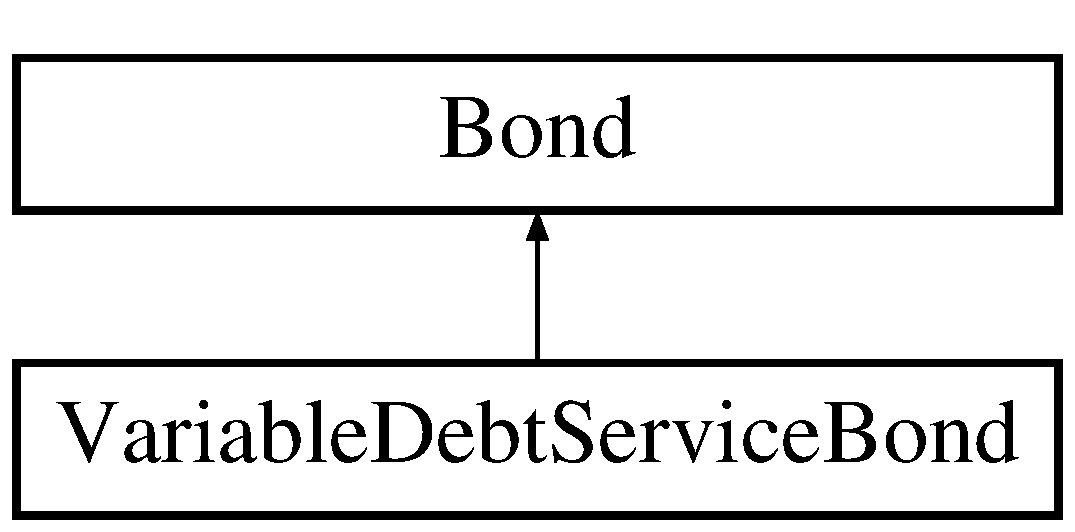
\includegraphics[height=2.000000cm]{classVariableDebtServiceBond}
\end{center}
\end{figure}
\subsection*{Public Member Functions}
\begin{DoxyCompactItemize}
\item 
\mbox{\hyperlink{classVariableDebtServiceBond_a8259b64265dd9701ac5888e0fe0bc565}{$\sim$\+Variable\+Debt\+Service\+Bond}} () override
\begin{DoxyCompactList}\small\item\em Destroys the variable debt service bond object. This destructor cleans up resources associated with the variable debt service bond. It is automatically called when an object of the {\ttfamily \mbox{\hyperlink{classVariableDebtServiceBond}{Variable\+Debt\+Service\+Bond}}} class goes out of scope or is deleted. \end{DoxyCompactList}\item 
double \mbox{\hyperlink{classVariableDebtServiceBond_a575a9a41df38e005ba0a1cff3eb2b921}{get\+Debt\+Service}} (int week) override
\begin{DoxyCompactList}\small\item\em Calculates and returns the debt service payment for a given week. This function calculates the debt service for the bond, checking if repayments are due and handling any corrections if the calculated debt service value is NaN. \end{DoxyCompactList}\item 
double \mbox{\hyperlink{classVariableDebtServiceBond_aa5ad4fcc7c65154105388b332ae98198}{get\+Present\+Value\+Debt\+Service}} (int week, double discount\+\_\+rate) override
\begin{DoxyCompactList}\small\item\em Calculates the present value of the debt service for a given week. \end{DoxyCompactList}\item 
double \mbox{\hyperlink{classVariableDebtServiceBond_a8cc7ee442d788b91b8c00e6bed07644d}{get\+Net\+Present\+Value\+At\+Issuance}} (double yearly\+\_\+discount\+\_\+rate, int week) const override
\begin{DoxyCompactList}\small\item\em Calculates the net present value (N\+PV) at issuance for the variable debt service bond. This calculation is generally not applicable for a variable rate bond and might require an additional calculation at the end of realization. This method is intended as a placeholder. \end{DoxyCompactList}\item 
void \mbox{\hyperlink{classVariableDebtServiceBond_a7d91921482f01d9bb37dba6e6d085771}{issue\+Bond}} (int week, int construction\+\_\+time, double bond\+\_\+term\+\_\+multiplier, double bond\+\_\+interest\+\_\+rate\+\_\+multiplier) override
\begin{DoxyCompactList}\small\item\em Issues the bond, initializes bond details, and calculates the variable debt service payment. This method calculates the initial variable debt service payment for the bond based on the bond\textquotesingle{}s cost of capital, debt fraction, coupon rate, and the number of payments. \end{DoxyCompactList}\item 
void \mbox{\hyperlink{classVariableDebtServiceBond_a692563150053b280f6e1ef23fd47c117}{set\+Debt\+Service}} (double updated\+\_\+allocated\+\_\+fraction\+\_\+of\+\_\+annual\+\_\+debt\+\_\+service) override
\begin{DoxyCompactList}\small\item\em Calculates and updates the variable debt service payment based on the provided allocated fraction of annual debt service. Overrides the virtual base class method. \end{DoxyCompactList}\item 
int \mbox{\hyperlink{classVariableDebtServiceBond_a3edee29f26e8ac74f9767770c6a951c9}{get\+Water\+Source\+ID}} () override
\begin{DoxyCompactList}\small\item\em Retrieves the water source ID associated with the bond. Overrides the virtual base class method. \end{DoxyCompactList}\end{DoxyCompactItemize}
\subsection*{Public Attributes}
\begin{DoxyCompactItemize}
\item 
Here’s the Sphinx style documentation for the Variable\+Debt\+Service\+Bond\+::\+Variable\+Debt\+Service\+Bond \mbox{\hyperlink{classVariableDebtServiceBond_a9369eb5b081c45a8608630b3eacae979}{constructor}}\+: \mbox{\hyperlink{classVariableDebtServiceBond}{Variable\+Debt\+Service\+Bond}}(const int \mbox{\hyperlink{classBond_a7f75bcafbc16676ad6dbafbf40afae4a}{id}}
\item 
Here’s the Sphinx style documentation for the Variable\+Debt\+Service\+Bond\+::\+Variable\+Debt\+Service\+Bond const int \mbox{\hyperlink{classVariableDebtServiceBond_a1b43195523e5571e04f2ed558497ab6a}{water\+\_\+source\+\_\+id}}
\item 
Here’s the Sphinx style documentation for the Variable\+Debt\+Service\+Bond\+::\+Variable\+Debt\+Service\+Bond const int const double \mbox{\hyperlink{classVariableDebtServiceBond_ac011dd32658be19f8dfc72e7d3b1e02c}{total\+\_\+unallocated\+\_\+cost\+\_\+of\+\_\+capital}}
\item 
Here’s the Sphinx style documentation for the Variable\+Debt\+Service\+Bond\+::\+Variable\+Debt\+Service\+Bond const int const double const double \mbox{\hyperlink{classVariableDebtServiceBond_a23f451bb14e4898aaa585fbeae9667f9}{initial\+\_\+fraction\+\_\+of\+\_\+allocated\+\_\+debt}}
\item 
Here’s the Sphinx style documentation for the Variable\+Debt\+Service\+Bond\+::\+Variable\+Debt\+Service\+Bond const int const double const double const int \mbox{\hyperlink{classVariableDebtServiceBond_ab4035559da3d8155d792612e628285ae}{n\+\_\+payments}}
\item 
Here’s the Sphinx style documentation for the Variable\+Debt\+Service\+Bond\+::\+Variable\+Debt\+Service\+Bond const int const double const double const int const double \mbox{\hyperlink{classVariableDebtServiceBond_a4062feaf0e15546bbcf575aa8ec372e0}{coupon\+\_\+rate}}
\item 
Here’s the Sphinx style documentation for the Variable\+Debt\+Service\+Bond\+::\+Variable\+Debt\+Service\+Bond const int const double const double const int const double vector$<$ int $>$ \mbox{\hyperlink{classVariableDebtServiceBond_a9ba0adce7f7b3f30e14e55837424ff7c}{pay\+\_\+on\+\_\+weeks}}
\item 
Here’s the Sphinx style documentation for the Variable\+Debt\+Service\+Bond\+::\+Variable\+Debt\+Service\+Bond const int const double const double const int const double vector$<$ int $>$ bool \mbox{\hyperlink{classVariableDebtServiceBond_a24b333de66efd610ef5d94a673250ff9}{begin\+\_\+repayment\+\_\+at\+\_\+issuance}} = false)
\end{DoxyCompactItemize}
\subsection*{Additional Inherited Members}


\subsection{Detailed Description}
Variable debt service bond class. This (municipal) bond has floating coupon payments that are adjusted at specified intervals. This bond is associated with a specific water source. 

\subsection{Constructor \& Destructor Documentation}
\mbox{\Hypertarget{classVariableDebtServiceBond_a8259b64265dd9701ac5888e0fe0bc565}\label{classVariableDebtServiceBond_a8259b64265dd9701ac5888e0fe0bc565}} 
\index{Variable\+Debt\+Service\+Bond@{Variable\+Debt\+Service\+Bond}!````~Variable\+Debt\+Service\+Bond@{$\sim$\+Variable\+Debt\+Service\+Bond}}
\index{````~Variable\+Debt\+Service\+Bond@{$\sim$\+Variable\+Debt\+Service\+Bond}!Variable\+Debt\+Service\+Bond@{Variable\+Debt\+Service\+Bond}}
\subsubsection{\texorpdfstring{$\sim$\+Variable\+Debt\+Service\+Bond()}{~VariableDebtServiceBond()}}
{\footnotesize\ttfamily Variable\+Debt\+Service\+Bond\+::$\sim$\+Variable\+Debt\+Service\+Bond (\begin{DoxyParamCaption}{ }\end{DoxyParamCaption})\hspace{0.3cm}{\ttfamily [override]}}



Destroys the variable debt service bond object. This destructor cleans up resources associated with the variable debt service bond. It is automatically called when an object of the {\ttfamily \mbox{\hyperlink{classVariableDebtServiceBond}{Variable\+Debt\+Service\+Bond}}} class goes out of scope or is deleted. 

\begin{DoxyReturn}{Returns}
None 
\end{DoxyReturn}


\subsection{Member Function Documentation}
\mbox{\Hypertarget{classVariableDebtServiceBond_a575a9a41df38e005ba0a1cff3eb2b921}\label{classVariableDebtServiceBond_a575a9a41df38e005ba0a1cff3eb2b921}} 
\index{Variable\+Debt\+Service\+Bond@{Variable\+Debt\+Service\+Bond}!get\+Debt\+Service@{get\+Debt\+Service}}
\index{get\+Debt\+Service@{get\+Debt\+Service}!Variable\+Debt\+Service\+Bond@{Variable\+Debt\+Service\+Bond}}
\subsubsection{\texorpdfstring{get\+Debt\+Service()}{getDebtService()}}
{\footnotesize\ttfamily double Variable\+Debt\+Service\+Bond\+::get\+Debt\+Service (\begin{DoxyParamCaption}\item[{int}]{week }\end{DoxyParamCaption})\hspace{0.3cm}{\ttfamily [override]}, {\ttfamily [virtual]}}



Calculates and returns the debt service payment for a given week. This function calculates the debt service for the bond, checking if repayments are due and handling any corrections if the calculated debt service value is NaN. 


\begin{DoxyParams}{Parameters}
{\em week} & The week number for which the debt service is to be calculated.\\
\hline
\end{DoxyParams}
\begin{DoxyReturn}{Returns}
double The calculated debt service for the specified week. If no payment is due for the week, returns 0. 
\end{DoxyReturn}


Implements \mbox{\hyperlink{classBond_a98d8ecaf4b36319674ebd220598996bc}{Bond}}.

\mbox{\Hypertarget{classVariableDebtServiceBond_a8cc7ee442d788b91b8c00e6bed07644d}\label{classVariableDebtServiceBond_a8cc7ee442d788b91b8c00e6bed07644d}} 
\index{Variable\+Debt\+Service\+Bond@{Variable\+Debt\+Service\+Bond}!get\+Net\+Present\+Value\+At\+Issuance@{get\+Net\+Present\+Value\+At\+Issuance}}
\index{get\+Net\+Present\+Value\+At\+Issuance@{get\+Net\+Present\+Value\+At\+Issuance}!Variable\+Debt\+Service\+Bond@{Variable\+Debt\+Service\+Bond}}
\subsubsection{\texorpdfstring{get\+Net\+Present\+Value\+At\+Issuance()}{getNetPresentValueAtIssuance()}}
{\footnotesize\ttfamily double Variable\+Debt\+Service\+Bond\+::get\+Net\+Present\+Value\+At\+Issuance (\begin{DoxyParamCaption}\item[{double}]{yearly\+\_\+discount\+\_\+rate,  }\item[{int}]{week }\end{DoxyParamCaption}) const\hspace{0.3cm}{\ttfamily [override]}, {\ttfamily [virtual]}}



Calculates the net present value (N\+PV) at issuance for the variable debt service bond. This calculation is generally not applicable for a variable rate bond and might require an additional calculation at the end of realization. This method is intended as a placeholder. 


\begin{DoxyParams}{Parameters}
{\em yearly\+\_\+discount\+\_\+rate} & The annual discount rate used for the N\+PV calculation. \\
\hline
{\em week} & The week number at which the N\+PV is to be calculated.\\
\hline
\end{DoxyParams}
\begin{DoxyReturn}{Returns}
double The calculated N\+PV at issuance. 
\end{DoxyReturn}


Implements \mbox{\hyperlink{classBond_a5997278813deb16aa5d01bbca8ecc7b2}{Bond}}.

\mbox{\Hypertarget{classVariableDebtServiceBond_aa5ad4fcc7c65154105388b332ae98198}\label{classVariableDebtServiceBond_aa5ad4fcc7c65154105388b332ae98198}} 
\index{Variable\+Debt\+Service\+Bond@{Variable\+Debt\+Service\+Bond}!get\+Present\+Value\+Debt\+Service@{get\+Present\+Value\+Debt\+Service}}
\index{get\+Present\+Value\+Debt\+Service@{get\+Present\+Value\+Debt\+Service}!Variable\+Debt\+Service\+Bond@{Variable\+Debt\+Service\+Bond}}
\subsubsection{\texorpdfstring{get\+Present\+Value\+Debt\+Service()}{getPresentValueDebtService()}}
{\footnotesize\ttfamily double Variable\+Debt\+Service\+Bond\+::get\+Present\+Value\+Debt\+Service (\begin{DoxyParamCaption}\item[{int}]{week,  }\item[{double}]{discount\+\_\+rate }\end{DoxyParamCaption})\hspace{0.3cm}{\ttfamily [override]}, {\ttfamily [virtual]}}



Calculates the present value of the debt service for a given week. 

This function calculates the present value of the debt service payment for a specific week, taking into account the discount rate. It checks if the bond is in its repayment phase, and if the current week is a designated payment week.


\begin{DoxyParams}{Parameters}
{\em week} & The current week for which the debt service present value is calculated. \\
\hline
{\em discount\+\_\+rate} & The annual discount rate used for present value calculations.\\
\hline
\end{DoxyParams}
\begin{DoxyReturn}{Returns}
double The present value of the debt service for the given week. 
\end{DoxyReturn}


Implements \mbox{\hyperlink{classBond_a322d4ab0c0c72824ac4df5df80f14d24}{Bond}}.

\mbox{\Hypertarget{classVariableDebtServiceBond_a3edee29f26e8ac74f9767770c6a951c9}\label{classVariableDebtServiceBond_a3edee29f26e8ac74f9767770c6a951c9}} 
\index{Variable\+Debt\+Service\+Bond@{Variable\+Debt\+Service\+Bond}!get\+Water\+Source\+ID@{get\+Water\+Source\+ID}}
\index{get\+Water\+Source\+ID@{get\+Water\+Source\+ID}!Variable\+Debt\+Service\+Bond@{Variable\+Debt\+Service\+Bond}}
\subsubsection{\texorpdfstring{get\+Water\+Source\+I\+D()}{getWaterSourceID()}}
{\footnotesize\ttfamily int Variable\+Debt\+Service\+Bond\+::get\+Water\+Source\+ID (\begin{DoxyParamCaption}{ }\end{DoxyParamCaption})\hspace{0.3cm}{\ttfamily [override]}, {\ttfamily [virtual]}}



Retrieves the water source ID associated with the bond. Overrides the virtual base class method. 

This function returns the water source ID that is associated with the bond. The ID can be used to track or link the bond to a specific water source.

\begin{DoxyReturn}{Returns}
int The water source ID associated with the bond. 
\end{DoxyReturn}


Reimplemented from \mbox{\hyperlink{classBond_a8190ab6482e6a9481afca4840147527e}{Bond}}.

\mbox{\Hypertarget{classVariableDebtServiceBond_a7d91921482f01d9bb37dba6e6d085771}\label{classVariableDebtServiceBond_a7d91921482f01d9bb37dba6e6d085771}} 
\index{Variable\+Debt\+Service\+Bond@{Variable\+Debt\+Service\+Bond}!issue\+Bond@{issue\+Bond}}
\index{issue\+Bond@{issue\+Bond}!Variable\+Debt\+Service\+Bond@{Variable\+Debt\+Service\+Bond}}
\subsubsection{\texorpdfstring{issue\+Bond()}{issueBond()}}
{\footnotesize\ttfamily void Variable\+Debt\+Service\+Bond\+::issue\+Bond (\begin{DoxyParamCaption}\item[{int}]{week,  }\item[{int}]{construction\+\_\+time,  }\item[{double}]{bond\+\_\+term\+\_\+multiplier,  }\item[{double}]{bond\+\_\+interest\+\_\+rate\+\_\+multiplier }\end{DoxyParamCaption})\hspace{0.3cm}{\ttfamily [override]}, {\ttfamily [virtual]}}



Issues the bond, initializes bond details, and calculates the variable debt service payment. This method calculates the initial variable debt service payment for the bond based on the bond\textquotesingle{}s cost of capital, debt fraction, coupon rate, and the number of payments. 


\begin{DoxyParams}{Parameters}
{\em week} & The week when the bond is issued. \\
\hline
{\em construction\+\_\+time} & The time (in weeks) it takes to complete construction. \\
\hline
{\em bond\+\_\+term\+\_\+multiplier} & A multiplier that adjusts the term of the bond. \\
\hline
{\em bond\+\_\+interest\+\_\+rate\+\_\+multiplier} & A multiplier that adjusts the interest rate of the bond.\\
\hline
\end{DoxyParams}
\begin{DoxyReturn}{Returns}
void 
\end{DoxyReturn}


Reimplemented from \mbox{\hyperlink{classBond_a726edbe3ea7047ebc7246585943763e3}{Bond}}.

\mbox{\Hypertarget{classVariableDebtServiceBond_a692563150053b280f6e1ef23fd47c117}\label{classVariableDebtServiceBond_a692563150053b280f6e1ef23fd47c117}} 
\index{Variable\+Debt\+Service\+Bond@{Variable\+Debt\+Service\+Bond}!set\+Debt\+Service@{set\+Debt\+Service}}
\index{set\+Debt\+Service@{set\+Debt\+Service}!Variable\+Debt\+Service\+Bond@{Variable\+Debt\+Service\+Bond}}
\subsubsection{\texorpdfstring{set\+Debt\+Service()}{setDebtService()}}
{\footnotesize\ttfamily void Variable\+Debt\+Service\+Bond\+::set\+Debt\+Service (\begin{DoxyParamCaption}\item[{double}]{updated\+\_\+allocated\+\_\+fraction\+\_\+of\+\_\+annual\+\_\+debt\+\_\+service }\end{DoxyParamCaption})\hspace{0.3cm}{\ttfamily [override]}, {\ttfamily [virtual]}}



Calculates and updates the variable debt service payment based on the provided allocated fraction of annual debt service. Overrides the virtual base class method. 


\begin{DoxyParams}{Parameters}
{\em updated\+\_\+allocated\+\_\+fraction\+\_\+of\+\_\+annual\+\_\+debt\+\_\+service} & The new fraction of the annual debt service to be allocated to the bond.\\
\hline
\end{DoxyParams}
\begin{DoxyReturn}{Returns}
void 
\end{DoxyReturn}


Reimplemented from \mbox{\hyperlink{classBond_aff7fc4e1edcf199fb592d22c765b854e}{Bond}}.



\subsection{Member Data Documentation}
\mbox{\Hypertarget{classVariableDebtServiceBond_a24b333de66efd610ef5d94a673250ff9}\label{classVariableDebtServiceBond_a24b333de66efd610ef5d94a673250ff9}} 
\index{Variable\+Debt\+Service\+Bond@{Variable\+Debt\+Service\+Bond}!begin\+\_\+repayment\+\_\+at\+\_\+issuance@{begin\+\_\+repayment\+\_\+at\+\_\+issuance}}
\index{begin\+\_\+repayment\+\_\+at\+\_\+issuance@{begin\+\_\+repayment\+\_\+at\+\_\+issuance}!Variable\+Debt\+Service\+Bond@{Variable\+Debt\+Service\+Bond}}
\subsubsection{\texorpdfstring{begin\+\_\+repayment\+\_\+at\+\_\+issuance}{begin\_repayment\_at\_issuance}}
{\footnotesize\ttfamily Here’s the Sphinx style documentation for the Variable\+Debt\+Service\+Bond\+::\+Variable\+Debt\+Service\+Bond const int const double const double const int const double vector$<$int$>$ bool Variable\+Debt\+Service\+Bond\+::begin\+\_\+repayment\+\_\+at\+\_\+issuance = false)}

\mbox{\Hypertarget{classVariableDebtServiceBond_a9369eb5b081c45a8608630b3eacae979}\label{classVariableDebtServiceBond_a9369eb5b081c45a8608630b3eacae979}} 
\index{Variable\+Debt\+Service\+Bond@{Variable\+Debt\+Service\+Bond}!constructor@{constructor}}
\index{constructor@{constructor}!Variable\+Debt\+Service\+Bond@{Variable\+Debt\+Service\+Bond}}
\subsubsection{\texorpdfstring{constructor}{constructor}}
{\footnotesize\ttfamily Here’s the Sphinx style documentation for the Variable\+Debt\+Service\+Bond\+::\+Variable\+Debt\+Service\+Bond Variable\+Debt\+Service\+Bond\+::constructor}

\mbox{\Hypertarget{classVariableDebtServiceBond_a4062feaf0e15546bbcf575aa8ec372e0}\label{classVariableDebtServiceBond_a4062feaf0e15546bbcf575aa8ec372e0}} 
\index{Variable\+Debt\+Service\+Bond@{Variable\+Debt\+Service\+Bond}!coupon\+\_\+rate@{coupon\+\_\+rate}}
\index{coupon\+\_\+rate@{coupon\+\_\+rate}!Variable\+Debt\+Service\+Bond@{Variable\+Debt\+Service\+Bond}}
\subsubsection{\texorpdfstring{coupon\+\_\+rate}{coupon\_rate}}
{\footnotesize\ttfamily Here’s the Sphinx style documentation for the Variable\+Debt\+Service\+Bond\+::\+Variable\+Debt\+Service\+Bond const int const double const double const int const double Variable\+Debt\+Service\+Bond\+::coupon\+\_\+rate}

\mbox{\Hypertarget{classVariableDebtServiceBond_a23f451bb14e4898aaa585fbeae9667f9}\label{classVariableDebtServiceBond_a23f451bb14e4898aaa585fbeae9667f9}} 
\index{Variable\+Debt\+Service\+Bond@{Variable\+Debt\+Service\+Bond}!initial\+\_\+fraction\+\_\+of\+\_\+allocated\+\_\+debt@{initial\+\_\+fraction\+\_\+of\+\_\+allocated\+\_\+debt}}
\index{initial\+\_\+fraction\+\_\+of\+\_\+allocated\+\_\+debt@{initial\+\_\+fraction\+\_\+of\+\_\+allocated\+\_\+debt}!Variable\+Debt\+Service\+Bond@{Variable\+Debt\+Service\+Bond}}
\subsubsection{\texorpdfstring{initial\+\_\+fraction\+\_\+of\+\_\+allocated\+\_\+debt}{initial\_fraction\_of\_allocated\_debt}}
{\footnotesize\ttfamily Here’s the Sphinx style documentation for the Variable\+Debt\+Service\+Bond\+::\+Variable\+Debt\+Service\+Bond const int const double const double Variable\+Debt\+Service\+Bond\+::initial\+\_\+fraction\+\_\+of\+\_\+allocated\+\_\+debt}

\mbox{\Hypertarget{classVariableDebtServiceBond_ab4035559da3d8155d792612e628285ae}\label{classVariableDebtServiceBond_ab4035559da3d8155d792612e628285ae}} 
\index{Variable\+Debt\+Service\+Bond@{Variable\+Debt\+Service\+Bond}!n\+\_\+payments@{n\+\_\+payments}}
\index{n\+\_\+payments@{n\+\_\+payments}!Variable\+Debt\+Service\+Bond@{Variable\+Debt\+Service\+Bond}}
\subsubsection{\texorpdfstring{n\+\_\+payments}{n\_payments}}
{\footnotesize\ttfamily Here’s the Sphinx style documentation for the Variable\+Debt\+Service\+Bond\+::\+Variable\+Debt\+Service\+Bond const int const double const double const int Variable\+Debt\+Service\+Bond\+::n\+\_\+payments}

\mbox{\Hypertarget{classVariableDebtServiceBond_a9ba0adce7f7b3f30e14e55837424ff7c}\label{classVariableDebtServiceBond_a9ba0adce7f7b3f30e14e55837424ff7c}} 
\index{Variable\+Debt\+Service\+Bond@{Variable\+Debt\+Service\+Bond}!pay\+\_\+on\+\_\+weeks@{pay\+\_\+on\+\_\+weeks}}
\index{pay\+\_\+on\+\_\+weeks@{pay\+\_\+on\+\_\+weeks}!Variable\+Debt\+Service\+Bond@{Variable\+Debt\+Service\+Bond}}
\subsubsection{\texorpdfstring{pay\+\_\+on\+\_\+weeks}{pay\_on\_weeks}}
{\footnotesize\ttfamily Here’s the Sphinx style documentation for the Variable\+Debt\+Service\+Bond\+::\+Variable\+Debt\+Service\+Bond const int const double const double const int const double vector$<$int$>$ Variable\+Debt\+Service\+Bond\+::pay\+\_\+on\+\_\+weeks}

\mbox{\Hypertarget{classVariableDebtServiceBond_ac011dd32658be19f8dfc72e7d3b1e02c}\label{classVariableDebtServiceBond_ac011dd32658be19f8dfc72e7d3b1e02c}} 
\index{Variable\+Debt\+Service\+Bond@{Variable\+Debt\+Service\+Bond}!total\+\_\+unallocated\+\_\+cost\+\_\+of\+\_\+capital@{total\+\_\+unallocated\+\_\+cost\+\_\+of\+\_\+capital}}
\index{total\+\_\+unallocated\+\_\+cost\+\_\+of\+\_\+capital@{total\+\_\+unallocated\+\_\+cost\+\_\+of\+\_\+capital}!Variable\+Debt\+Service\+Bond@{Variable\+Debt\+Service\+Bond}}
\subsubsection{\texorpdfstring{total\+\_\+unallocated\+\_\+cost\+\_\+of\+\_\+capital}{total\_unallocated\_cost\_of\_capital}}
{\footnotesize\ttfamily Here’s the Sphinx style documentation for the Variable\+Debt\+Service\+Bond\+::\+Variable\+Debt\+Service\+Bond const int const double Variable\+Debt\+Service\+Bond\+::total\+\_\+unallocated\+\_\+cost\+\_\+of\+\_\+capital}

\mbox{\Hypertarget{classVariableDebtServiceBond_a1b43195523e5571e04f2ed558497ab6a}\label{classVariableDebtServiceBond_a1b43195523e5571e04f2ed558497ab6a}} 
\index{Variable\+Debt\+Service\+Bond@{Variable\+Debt\+Service\+Bond}!water\+\_\+source\+\_\+id@{water\+\_\+source\+\_\+id}}
\index{water\+\_\+source\+\_\+id@{water\+\_\+source\+\_\+id}!Variable\+Debt\+Service\+Bond@{Variable\+Debt\+Service\+Bond}}
\subsubsection{\texorpdfstring{water\+\_\+source\+\_\+id}{water\_source\_id}}
{\footnotesize\ttfamily Here’s the Sphinx style documentation for the Variable\+Debt\+Service\+Bond\+::\+Variable\+Debt\+Service\+Bond const int Variable\+Debt\+Service\+Bond\+::water\+\_\+source\+\_\+id}



The documentation for this class was generated from the following file\+:\begin{DoxyCompactItemize}
\item 
/home/fs02/pmr82\+\_\+0001/lbl59/\+Water\+Paths-\/doc/src/\+System\+Components/\+Bonds/\mbox{\hyperlink{VariableDebtServiceBond_8h}{Variable\+Debt\+Service\+Bond.\+h}}\end{DoxyCompactItemize}

\hypertarget{classVariableJointWTP}{}\section{Variable\+Joint\+W\+TP Class Reference}
\label{classVariableJointWTP}\index{Variable\+Joint\+W\+TP@{Variable\+Joint\+W\+TP}}


This is a subclass of \mbox{\hyperlink{classJointWTP}{Joint\+W\+TP}} that allows for variable allocations of treatment capacity to utilities. The \mbox{\hyperlink{classJointWTP}{Joint\+W\+TP}} subclass is in turn a subclass of \mbox{\hyperlink{classWaterSource}{Water\+Source}}.  




{\ttfamily \#include $<$Variable\+Joint\+W\+T\+P.\+h$>$}

Inheritance diagram for Variable\+Joint\+W\+TP\+:\begin{figure}[H]
\begin{center}
\leavevmode
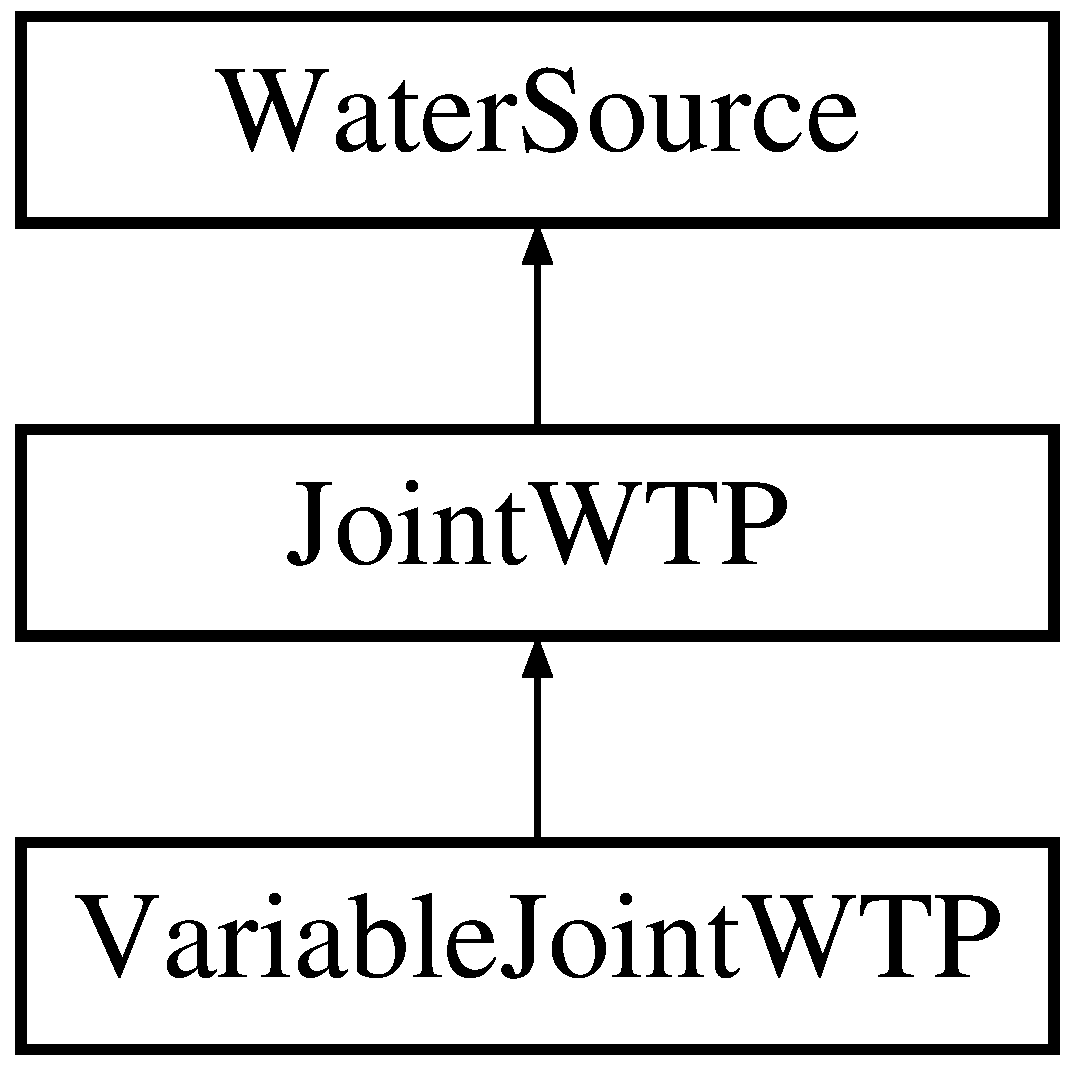
\includegraphics[height=3.000000cm]{classVariableJointWTP}
\end{center}
\end{figure}
\subsection*{Public Member Functions}
\begin{DoxyCompactItemize}
\item 
\mbox{\hyperlink{classVariableJointWTP_a26fa2204e90fb7e44f17dbd2958a56fc}{Variable\+Joint\+W\+TP}} (const char $\ast$\mbox{\hyperlink{classWaterSource_a846ea74c5b453d014f594d41fee8c765}{name}}, const int \mbox{\hyperlink{classWaterSource_a6eafe5dfefd317877d1244e8a7c6e742}{id}}, const int \mbox{\hyperlink{classJointWTP_aa5830cb4d3013a004b7168f4dbf475eb}{parent\+\_\+reservoir\+\_\+\+ID}}, const int \mbox{\hyperlink{classJointWTP_a0e10a7f7ade04d5f3572f185de1b8653}{expansion\+\_\+sequence\+\_\+id}}, const double \mbox{\hyperlink{classWaterSource_a2fdfd5ff7d103e71108cf2a31babaccb}{total\+\_\+treatment\+\_\+capacity}}, vector$<$ int $>$ connected\+\_\+sources, vector$<$ int $>$ \&agreement\+\_\+utility\+\_\+ids, vector$<$ double $>$ \&initial\+\_\+treatment\+\_\+capacity\+\_\+allocations, vector$<$ \mbox{\hyperlink{classBond}{Bond}} $\ast$$>$ \&\mbox{\hyperlink{classWaterSource_a413b094e11bdce62f4d82e5bb9e4706e}{bonds}}, const vector$<$ double $>$ \&construction\+\_\+time\+\_\+range, double permitting\+\_\+period)
\begin{DoxyCompactList}\small\item\em Constructs a {\ttfamily \mbox{\hyperlink{classVariableJointWTP}{Variable\+Joint\+W\+TP}}} object with the specified parameters. \end{DoxyCompactList}\item 
\mbox{\hyperlink{classVariableJointWTP_afb1491d02ab8f69966b5dda871dadb34}{Variable\+Joint\+W\+TP}} (const \mbox{\hyperlink{classVariableJointWTP}{Variable\+Joint\+W\+TP}} \&variable\+\_\+joint\+\_\+water\+\_\+treatment\+\_\+plant)
\begin{DoxyCompactList}\small\item\em Copy constructor for the {\ttfamily \mbox{\hyperlink{classVariableJointWTP}{Variable\+Joint\+W\+TP}}} class. \end{DoxyCompactList}\item 
\mbox{\hyperlink{classVariableJointWTP_aaa9eccc2b254ebe82769cc90bed5b893}{$\sim$\+Variable\+Joint\+W\+TP}} () override
\begin{DoxyCompactList}\small\item\em Destructor for the {\ttfamily \mbox{\hyperlink{classVariableJointWTP}{Variable\+Joint\+W\+TP}}} class. \end{DoxyCompactList}\item 
\mbox{\hyperlink{classVariableJointWTP}{Variable\+Joint\+W\+TP}} \& \mbox{\hyperlink{classVariableJointWTP_acb9e62cc3198df8df6c7ac87c7f7a4cd}{operator=}} (const \mbox{\hyperlink{classVariableJointWTP}{Variable\+Joint\+W\+TP}} \&variable\+\_\+joint\+\_\+water\+\_\+treatment\+\_\+plant)
\begin{DoxyCompactList}\small\item\em Assignment operator for copying data for another {\ttfamily \mbox{\hyperlink{classVariableJointWTP}{Variable\+Joint\+W\+TP}}} object. \end{DoxyCompactList}\item 
void \mbox{\hyperlink{classVariableJointWTP_ab20f14dccd7079f546984d7bf1c00a71}{apply\+Continuity}} (int week, double \mbox{\hyperlink{classWaterSource_a7a69b2e9b6030f1035e6cf44d2918ee5}{upstream\+\_\+source\+\_\+inflow}}, double wastewater\+\_\+discharge, vector$<$ double $>$ \&demand\+\_\+outflow) override
\begin{DoxyCompactList}\small\item\em Applies continuity for the {\ttfamily \mbox{\hyperlink{classVariableJointWTP}{Variable\+Joint\+W\+TP}}} class. \end{DoxyCompactList}\item 
double \mbox{\hyperlink{classVariableJointWTP_ade062353af947456c6a3ed10a93686d4}{implement\+Initial\+Treatment\+Capacity}} (int utility\+\_\+id) override
\begin{DoxyCompactList}\small\item\em Implements the initial treatment capacity for a specific utility. \end{DoxyCompactList}\item 
void \mbox{\hyperlink{classVariableJointWTP_ab02c6701ad5120e189023b038bae13b7}{reset\+Allocations}} (const vector$<$ double $>$ $\ast$demand\+\_\+ratios) override
\begin{DoxyCompactList}\small\item\em Resets the treatment allocations based on demand deltas for the utilities. \end{DoxyCompactList}\end{DoxyCompactItemize}
\subsection*{Additional Inherited Members}


\subsection{Detailed Description}
This is a subclass of \mbox{\hyperlink{classJointWTP}{Joint\+W\+TP}} that allows for variable allocations of treatment capacity to utilities. The \mbox{\hyperlink{classJointWTP}{Joint\+W\+TP}} subclass is in turn a subclass of \mbox{\hyperlink{classWaterSource}{Water\+Source}}. 

Created by dgorelic on 10/29/2019.

F\+I\+X\+ME\+: Unclear what the purpose of this class is and how it differs from \mbox{\hyperlink{classJointWTP}{Joint\+W\+TP}}. 

\subsection{Constructor \& Destructor Documentation}
\mbox{\Hypertarget{classVariableJointWTP_a26fa2204e90fb7e44f17dbd2958a56fc}\label{classVariableJointWTP_a26fa2204e90fb7e44f17dbd2958a56fc}} 
\index{Variable\+Joint\+W\+TP@{Variable\+Joint\+W\+TP}!Variable\+Joint\+W\+TP@{Variable\+Joint\+W\+TP}}
\index{Variable\+Joint\+W\+TP@{Variable\+Joint\+W\+TP}!Variable\+Joint\+W\+TP@{Variable\+Joint\+W\+TP}}
\subsubsection{\texorpdfstring{Variable\+Joint\+W\+T\+P()}{VariableJointWTP()}\hspace{0.1cm}{\footnotesize\ttfamily [1/2]}}
{\footnotesize\ttfamily Variable\+Joint\+W\+T\+P\+::\+Variable\+Joint\+W\+TP (\begin{DoxyParamCaption}\item[{const char $\ast$}]{name,  }\item[{const int}]{id,  }\item[{const int}]{parent\+\_\+reservoir\+\_\+\+ID,  }\item[{const int}]{expansion\+\_\+sequence\+\_\+id,  }\item[{const double}]{total\+\_\+treatment\+\_\+capacity,  }\item[{vector$<$ int $>$}]{connected\+\_\+sources,  }\item[{vector$<$ int $>$ \&}]{agreement\+\_\+utility\+\_\+ids,  }\item[{vector$<$ double $>$ \&}]{initial\+\_\+treatment\+\_\+capacity\+\_\+allocations,  }\item[{vector$<$ \mbox{\hyperlink{classBond}{Bond}} $\ast$$>$ \&}]{bonds,  }\item[{const vector$<$ double $>$ \&}]{construction\+\_\+time\+\_\+range,  }\item[{double}]{permitting\+\_\+period }\end{DoxyParamCaption})}



Constructs a {\ttfamily \mbox{\hyperlink{classVariableJointWTP}{Variable\+Joint\+W\+TP}}} object with the specified parameters. 

This constructor initializes a {\ttfamily \mbox{\hyperlink{classVariableJointWTP}{Variable\+Joint\+W\+TP}}} object, which represents a joint water treatment plant with variable treatment capacity allocations, and associates it with a specific parent reservoir.


\begin{DoxyParams}{Parameters}
{\em name} & The name of the joint water treatment plant. \\
\hline
{\em id} & The ID of the joint water treatment plant. \\
\hline
{\em parent\+\_\+reservoir\+\_\+\+ID} & The ID of the parent reservoir for the joint water treatment plant. \\
\hline
{\em expansion\+\_\+sequence\+\_\+id} & The expansion sequence ID for the joint water treatment plant. \\
\hline
{\em total\+\_\+treatment\+\_\+capacity} & The total treatment capacity of the plant. \\
\hline
{\em connected\+\_\+sources} & A list of source I\+Ds connected to the plant. \\
\hline
{\em agreement\+\_\+utility\+\_\+ids} & A list of utility I\+Ds that have agreements with the plant. \\
\hline
{\em initial\+\_\+treatment\+\_\+capacity\+\_\+allocations} & A list of initial treatment capacity allocations for each utility. \\
\hline
{\em bonds} & A list of bonds associated with the plant. \\
\hline
{\em construction\+\_\+time\+\_\+range} & A vector specifying the time range for construction. \\
\hline
{\em permitting\+\_\+period} & The permitting period for the plant. \\
\hline
\end{DoxyParams}
\mbox{\Hypertarget{classVariableJointWTP_afb1491d02ab8f69966b5dda871dadb34}\label{classVariableJointWTP_afb1491d02ab8f69966b5dda871dadb34}} 
\index{Variable\+Joint\+W\+TP@{Variable\+Joint\+W\+TP}!Variable\+Joint\+W\+TP@{Variable\+Joint\+W\+TP}}
\index{Variable\+Joint\+W\+TP@{Variable\+Joint\+W\+TP}!Variable\+Joint\+W\+TP@{Variable\+Joint\+W\+TP}}
\subsubsection{\texorpdfstring{Variable\+Joint\+W\+T\+P()}{VariableJointWTP()}\hspace{0.1cm}{\footnotesize\ttfamily [2/2]}}
{\footnotesize\ttfamily Variable\+Joint\+W\+T\+P\+::\+Variable\+Joint\+W\+TP (\begin{DoxyParamCaption}\item[{const \mbox{\hyperlink{classVariableJointWTP}{Variable\+Joint\+W\+TP}} \&}]{variable\+\_\+joint\+\_\+water\+\_\+treatment\+\_\+plant }\end{DoxyParamCaption})}



Copy constructor for the {\ttfamily \mbox{\hyperlink{classVariableJointWTP}{Variable\+Joint\+W\+TP}}} class. 

This constructor creates a new {\ttfamily \mbox{\hyperlink{classVariableJointWTP}{Variable\+Joint\+W\+TP}}} object as a copy of an existing one, inheriting the properties and treatment capacity allocations from the original plant.


\begin{DoxyParams}{Parameters}
{\em variable\+\_\+joint\+\_\+water\+\_\+treatment\+\_\+plant} & The {\ttfamily \mbox{\hyperlink{classVariableJointWTP}{Variable\+Joint\+W\+TP}}} object to copy from. \\
\hline
\end{DoxyParams}
\mbox{\Hypertarget{classVariableJointWTP_aaa9eccc2b254ebe82769cc90bed5b893}\label{classVariableJointWTP_aaa9eccc2b254ebe82769cc90bed5b893}} 
\index{Variable\+Joint\+W\+TP@{Variable\+Joint\+W\+TP}!````~Variable\+Joint\+W\+TP@{$\sim$\+Variable\+Joint\+W\+TP}}
\index{````~Variable\+Joint\+W\+TP@{$\sim$\+Variable\+Joint\+W\+TP}!Variable\+Joint\+W\+TP@{Variable\+Joint\+W\+TP}}
\subsubsection{\texorpdfstring{$\sim$\+Variable\+Joint\+W\+T\+P()}{~VariableJointWTP()}}
{\footnotesize\ttfamily Variable\+Joint\+W\+T\+P\+::$\sim$\+Variable\+Joint\+W\+TP (\begin{DoxyParamCaption}{ }\end{DoxyParamCaption})\hspace{0.3cm}{\ttfamily [override]}}



Destructor for the {\ttfamily \mbox{\hyperlink{classVariableJointWTP}{Variable\+Joint\+W\+TP}}} class. 

This function cleans up resources used by the \mbox{\hyperlink{classQuarry}{Quarry}} object. Since the class does not dynamically allocate resources directly, the destructor relies on the base class ({\ttfamily \mbox{\hyperlink{classWaterSource}{Water\+Source}}}) and standard cleanup mechanisms. 

\subsection{Member Function Documentation}
\mbox{\Hypertarget{classVariableJointWTP_ab20f14dccd7079f546984d7bf1c00a71}\label{classVariableJointWTP_ab20f14dccd7079f546984d7bf1c00a71}} 
\index{Variable\+Joint\+W\+TP@{Variable\+Joint\+W\+TP}!apply\+Continuity@{apply\+Continuity}}
\index{apply\+Continuity@{apply\+Continuity}!Variable\+Joint\+W\+TP@{Variable\+Joint\+W\+TP}}
\subsubsection{\texorpdfstring{apply\+Continuity()}{applyContinuity()}}
{\footnotesize\ttfamily void Variable\+Joint\+W\+T\+P\+::apply\+Continuity (\begin{DoxyParamCaption}\item[{int}]{week,  }\item[{double}]{upstream\+\_\+source\+\_\+inflow,  }\item[{double}]{wastewater\+\_\+discharge,  }\item[{vector$<$ double $>$ \&}]{demand\+\_\+outflow }\end{DoxyParamCaption})\hspace{0.3cm}{\ttfamily [override]}, {\ttfamily [virtual]}}



Applies continuity for the {\ttfamily \mbox{\hyperlink{classVariableJointWTP}{Variable\+Joint\+W\+TP}}} class. 

This function calls the base class {\ttfamily \mbox{\hyperlink{classJointWTP}{Joint\+W\+TP}}}\textquotesingle{}s {\ttfamily apply\+Continuity} method to perform the continuity calculations for the water treatment plant, considering the upstream inflow, wastewater discharge, and demand outflow.


\begin{DoxyParams}{Parameters}
{\em week} & The week for which the continuity is applied. \\
\hline
{\em upstream\+\_\+source\+\_\+inflow} & The inflow from the upstream source. \\
\hline
{\em wastewater\+\_\+discharge} & The discharge of wastewater into the plant. \\
\hline
{\em demand\+\_\+outflow} & A vector containing the demand outflow for each utility. \\
\hline
\end{DoxyParams}


Reimplemented from \mbox{\hyperlink{classJointWTP_a07106b573ea34386621a95d3fbcafd1a}{Joint\+W\+TP}}.

\mbox{\Hypertarget{classVariableJointWTP_ade062353af947456c6a3ed10a93686d4}\label{classVariableJointWTP_ade062353af947456c6a3ed10a93686d4}} 
\index{Variable\+Joint\+W\+TP@{Variable\+Joint\+W\+TP}!implement\+Initial\+Treatment\+Capacity@{implement\+Initial\+Treatment\+Capacity}}
\index{implement\+Initial\+Treatment\+Capacity@{implement\+Initial\+Treatment\+Capacity}!Variable\+Joint\+W\+TP@{Variable\+Joint\+W\+TP}}
\subsubsection{\texorpdfstring{implement\+Initial\+Treatment\+Capacity()}{implementInitialTreatmentCapacity()}}
{\footnotesize\ttfamily double Variable\+Joint\+W\+T\+P\+::implement\+Initial\+Treatment\+Capacity (\begin{DoxyParamCaption}\item[{int}]{utility\+\_\+id }\end{DoxyParamCaption})\hspace{0.3cm}{\ttfamily [override]}, {\ttfamily [virtual]}}



Implements the initial treatment capacity for a specific utility. 

This function returns the treatment capacity allocated to a utility based on the initial treatment allocations.


\begin{DoxyParams}{Parameters}
{\em utility\+\_\+id} & The ID of the utility for which the treatment capacity is retrieved.\\
\hline
\end{DoxyParams}
\begin{DoxyReturn}{Returns}
The initial treatment capacity allocated to the specified utility. 
\end{DoxyReturn}


Reimplemented from \mbox{\hyperlink{classJointWTP_ae8a2a5c4d5173b43d30fc9c1169574f8}{Joint\+W\+TP}}.

\mbox{\Hypertarget{classVariableJointWTP_acb9e62cc3198df8df6c7ac87c7f7a4cd}\label{classVariableJointWTP_acb9e62cc3198df8df6c7ac87c7f7a4cd}} 
\index{Variable\+Joint\+W\+TP@{Variable\+Joint\+W\+TP}!operator=@{operator=}}
\index{operator=@{operator=}!Variable\+Joint\+W\+TP@{Variable\+Joint\+W\+TP}}
\subsubsection{\texorpdfstring{operator=()}{operator=()}}
{\footnotesize\ttfamily \mbox{\hyperlink{classVariableJointWTP}{Variable\+Joint\+W\+TP}}\& Variable\+Joint\+W\+T\+P\+::operator= (\begin{DoxyParamCaption}\item[{const \mbox{\hyperlink{classVariableJointWTP}{Variable\+Joint\+W\+TP}} \&}]{variable\+\_\+joint\+\_\+water\+\_\+treatment\+\_\+plant }\end{DoxyParamCaption})}



Assignment operator for copying data for another {\ttfamily \mbox{\hyperlink{classVariableJointWTP}{Variable\+Joint\+W\+TP}}} object. 

This operator assigns the values from another {\ttfamily \mbox{\hyperlink{classVariableJointWTP}{Variable\+Joint\+W\+TP}}} object to the current object, copying the storage area curve and performing a deep copy of the evaporation series. The base class {\ttfamily \mbox{\hyperlink{classWaterSource}{Water\+Source}}}\textquotesingle{}s assignment operator is also called to copy its attributes.


\begin{DoxyParams}{Parameters}
{\em variable\+\_\+joint\+\_\+water\+\_\+treatment\+\_\+plant} & The {\ttfamily \mbox{\hyperlink{classVariableJointWTP}{Variable\+Joint\+W\+TP}}} object to copy data from.\\
\hline
\end{DoxyParams}
\begin{DoxyReturn}{Returns}
A reference to the current {\ttfamily \mbox{\hyperlink{classVariableJointWTP}{Variable\+Joint\+W\+TP}}} object after assignment. 
\end{DoxyReturn}
\mbox{\Hypertarget{classVariableJointWTP_ab02c6701ad5120e189023b038bae13b7}\label{classVariableJointWTP_ab02c6701ad5120e189023b038bae13b7}} 
\index{Variable\+Joint\+W\+TP@{Variable\+Joint\+W\+TP}!reset\+Allocations@{reset\+Allocations}}
\index{reset\+Allocations@{reset\+Allocations}!Variable\+Joint\+W\+TP@{Variable\+Joint\+W\+TP}}
\subsubsection{\texorpdfstring{reset\+Allocations()}{resetAllocations()}}
{\footnotesize\ttfamily void Variable\+Joint\+W\+T\+P\+::reset\+Allocations (\begin{DoxyParamCaption}\item[{const vector$<$ double $>$ $\ast$}]{demand\+\_\+ratios }\end{DoxyParamCaption})\hspace{0.3cm}{\ttfamily [override]}, {\ttfamily [virtual]}}



Resets the treatment allocations based on demand deltas for the utilities. 

This function updates the treatment capacity allocations for each utility based on changes in demand. It adjusts the treatment allocations for the current year based on the estimated future demand deltas. If the allocations exceed the total treatment capacity, the fractions and capacities are adjusted accordingly to ensure proper allocation.


\begin{DoxyParams}{Parameters}
{\em demand\+\_\+deltas} & A vector containing the estimated demand changes for each utility. \\
\hline
\end{DoxyParams}


Reimplemented from \mbox{\hyperlink{classWaterSource_afe2f6b96383abdb14563db279a261a31}{Water\+Source}}.



The documentation for this class was generated from the following file\+:\begin{DoxyCompactItemize}
\item 
/home/fs02/pmr82\+\_\+0001/lbl59/\+Water\+Paths-\/doc/src/\+System\+Components/\+Water\+Sources/\mbox{\hyperlink{VariableJointWTP_8h}{Variable\+Joint\+W\+T\+P.\+h}}\end{DoxyCompactItemize}

\hypertarget{classWaterReuse}{}\section{Water\+Reuse Class Reference}
\label{classWaterReuse}\index{Water\+Reuse@{Water\+Reuse}}


{\ttfamily \#include $<$Water\+Reuse.\+h$>$}

Inheritance diagram for Water\+Reuse\+:\begin{figure}[H]
\begin{center}
\leavevmode
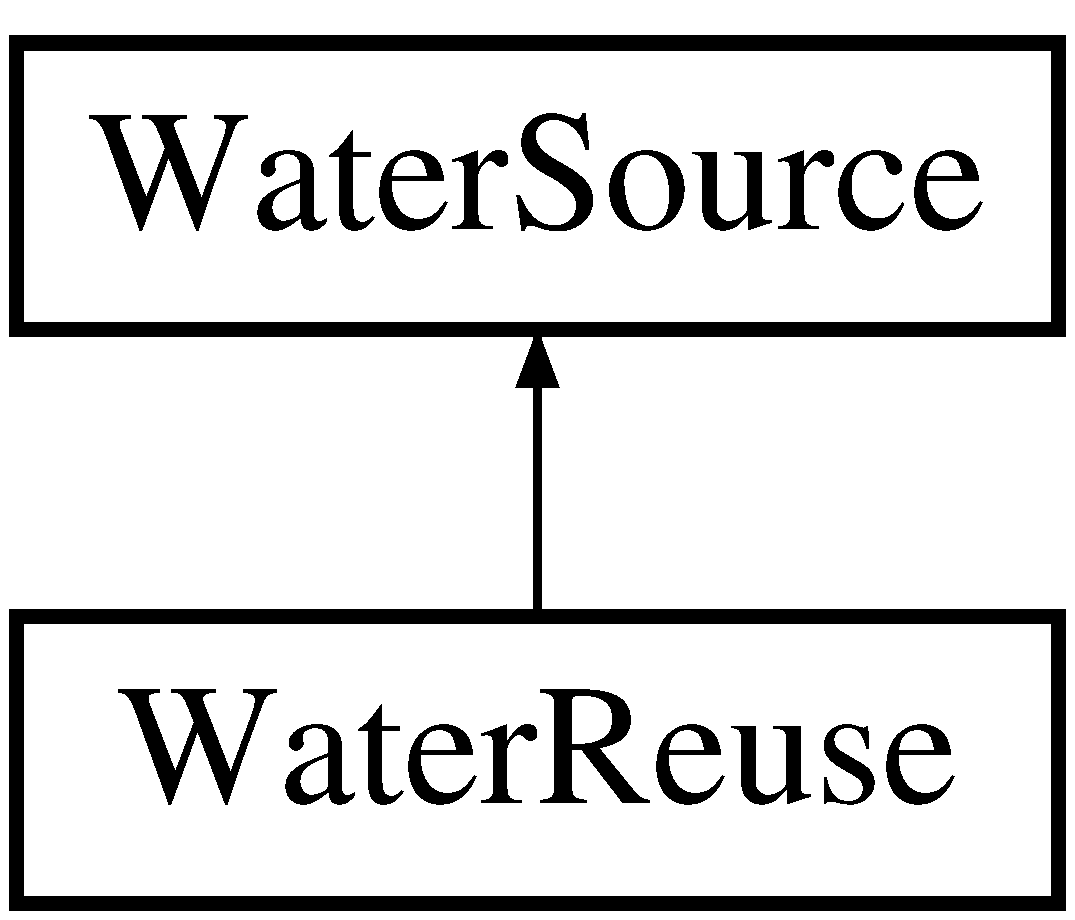
\includegraphics[height=2.000000cm]{classWaterReuse}
\end{center}
\end{figure}
\subsection*{Public Member Functions}
\begin{DoxyCompactItemize}
\item 
\mbox{\hyperlink{classWaterReuse_a0493da65856f50fad2bc2d2c087f378f}{Water\+Reuse}} (const char $\ast$\mbox{\hyperlink{classWaterSource_a846ea74c5b453d014f594d41fee8c765}{name}}, const int \mbox{\hyperlink{classWaterSource_a6eafe5dfefd317877d1244e8a7c6e742}{id}}, const double \mbox{\hyperlink{classWaterSource_a2ec257b415b248214a8bce7fc5267723}{capacity}})
\item 
\mbox{\hyperlink{classWaterReuse_a107ecd54d6fd705f0c31e57de21914e1}{Water\+Reuse}} (const char $\ast$\mbox{\hyperlink{classWaterSource_a846ea74c5b453d014f594d41fee8c765}{name}}, const int \mbox{\hyperlink{classWaterSource_a6eafe5dfefd317877d1244e8a7c6e742}{id}}, const double treatment\+\_\+capacity, const vector$<$ double $>$ \&construction\+\_\+time\+\_\+range, double permitting\+\_\+period, \mbox{\hyperlink{classBond}{Bond}} \&bond)
\item 
\mbox{\hyperlink{classWaterReuse_abe522bfe68c8b0bd05c4e608f3f6e6ba}{Water\+Reuse}} (const \mbox{\hyperlink{classWaterReuse}{Water\+Reuse}} \&reuse)
\item 
void \mbox{\hyperlink{classWaterReuse_ab8ffb10c69790047a3a5dda66cfaf3ee}{apply\+Continuity}} (int week, double \mbox{\hyperlink{classWaterSource_a7a69b2e9b6030f1035e6cf44d2918ee5}{upstream\+\_\+source\+\_\+inflow}}, double wastewater\+\_\+discharge, vector$<$ double $>$ \&demand\+\_\+outflow) override
\item 
\mbox{\hyperlink{classWaterReuse}{Water\+Reuse}} \& \mbox{\hyperlink{classWaterReuse_a8bf201adfc25021511d8844cd056d5bf}{operator=}} (const \mbox{\hyperlink{classWaterReuse}{Water\+Reuse}} \&water\+\_\+reuse)
\item 
double \mbox{\hyperlink{classWaterReuse_a78c905f77ca46fbbb2251f9cfa9a04de}{get\+Reused\+\_\+volume}} () const
\end{DoxyCompactItemize}
\subsection*{Additional Inherited Members}


\subsection{Constructor \& Destructor Documentation}
\mbox{\Hypertarget{classWaterReuse_a0493da65856f50fad2bc2d2c087f378f}\label{classWaterReuse_a0493da65856f50fad2bc2d2c087f378f}} 
\index{Water\+Reuse@{Water\+Reuse}!Water\+Reuse@{Water\+Reuse}}
\index{Water\+Reuse@{Water\+Reuse}!Water\+Reuse@{Water\+Reuse}}
\subsubsection{\texorpdfstring{Water\+Reuse()}{WaterReuse()}\hspace{0.1cm}{\footnotesize\ttfamily [1/3]}}
{\footnotesize\ttfamily Water\+Reuse\+::\+Water\+Reuse (\begin{DoxyParamCaption}\item[{const char $\ast$}]{name,  }\item[{const int}]{id,  }\item[{const double}]{capacity }\end{DoxyParamCaption})}

\mbox{\Hypertarget{classWaterReuse_a107ecd54d6fd705f0c31e57de21914e1}\label{classWaterReuse_a107ecd54d6fd705f0c31e57de21914e1}} 
\index{Water\+Reuse@{Water\+Reuse}!Water\+Reuse@{Water\+Reuse}}
\index{Water\+Reuse@{Water\+Reuse}!Water\+Reuse@{Water\+Reuse}}
\subsubsection{\texorpdfstring{Water\+Reuse()}{WaterReuse()}\hspace{0.1cm}{\footnotesize\ttfamily [2/3]}}
{\footnotesize\ttfamily Water\+Reuse\+::\+Water\+Reuse (\begin{DoxyParamCaption}\item[{const char $\ast$}]{name,  }\item[{const int}]{id,  }\item[{const double}]{treatment\+\_\+capacity,  }\item[{const vector$<$ double $>$ \&}]{construction\+\_\+time\+\_\+range,  }\item[{double}]{permitting\+\_\+period,  }\item[{\mbox{\hyperlink{classBond}{Bond}} \&}]{bond }\end{DoxyParamCaption})}

\mbox{\Hypertarget{classWaterReuse_abe522bfe68c8b0bd05c4e608f3f6e6ba}\label{classWaterReuse_abe522bfe68c8b0bd05c4e608f3f6e6ba}} 
\index{Water\+Reuse@{Water\+Reuse}!Water\+Reuse@{Water\+Reuse}}
\index{Water\+Reuse@{Water\+Reuse}!Water\+Reuse@{Water\+Reuse}}
\subsubsection{\texorpdfstring{Water\+Reuse()}{WaterReuse()}\hspace{0.1cm}{\footnotesize\ttfamily [3/3]}}
{\footnotesize\ttfamily Water\+Reuse\+::\+Water\+Reuse (\begin{DoxyParamCaption}\item[{const \mbox{\hyperlink{classWaterReuse}{Water\+Reuse}} \&}]{reuse }\end{DoxyParamCaption})}



\subsection{Member Function Documentation}
\mbox{\Hypertarget{classWaterReuse_ab8ffb10c69790047a3a5dda66cfaf3ee}\label{classWaterReuse_ab8ffb10c69790047a3a5dda66cfaf3ee}} 
\index{Water\+Reuse@{Water\+Reuse}!apply\+Continuity@{apply\+Continuity}}
\index{apply\+Continuity@{apply\+Continuity}!Water\+Reuse@{Water\+Reuse}}
\subsubsection{\texorpdfstring{apply\+Continuity()}{applyContinuity()}}
{\footnotesize\ttfamily void Water\+Reuse\+::apply\+Continuity (\begin{DoxyParamCaption}\item[{int}]{week,  }\item[{double}]{upstream\+\_\+source\+\_\+inflow,  }\item[{double}]{wastewater\+\_\+discharge,  }\item[{vector$<$ double $>$ \&}]{demand\+\_\+outflow }\end{DoxyParamCaption})\hspace{0.3cm}{\ttfamily [override]}, {\ttfamily [virtual]}}



Implements \mbox{\hyperlink{classWaterSource_ac070445379fe706f65b977dade4f3fbc}{Water\+Source}}.

\mbox{\Hypertarget{classWaterReuse_a78c905f77ca46fbbb2251f9cfa9a04de}\label{classWaterReuse_a78c905f77ca46fbbb2251f9cfa9a04de}} 
\index{Water\+Reuse@{Water\+Reuse}!get\+Reused\+\_\+volume@{get\+Reused\+\_\+volume}}
\index{get\+Reused\+\_\+volume@{get\+Reused\+\_\+volume}!Water\+Reuse@{Water\+Reuse}}
\subsubsection{\texorpdfstring{get\+Reused\+\_\+volume()}{getReused\_volume()}}
{\footnotesize\ttfamily double Water\+Reuse\+::get\+Reused\+\_\+volume (\begin{DoxyParamCaption}{ }\end{DoxyParamCaption}) const}

\mbox{\Hypertarget{classWaterReuse_a8bf201adfc25021511d8844cd056d5bf}\label{classWaterReuse_a8bf201adfc25021511d8844cd056d5bf}} 
\index{Water\+Reuse@{Water\+Reuse}!operator=@{operator=}}
\index{operator=@{operator=}!Water\+Reuse@{Water\+Reuse}}
\subsubsection{\texorpdfstring{operator=()}{operator=()}}
{\footnotesize\ttfamily \mbox{\hyperlink{classWaterReuse}{Water\+Reuse}} \& Water\+Reuse\+::operator= (\begin{DoxyParamCaption}\item[{const \mbox{\hyperlink{classWaterReuse}{Water\+Reuse}} \&}]{water\+\_\+reuse }\end{DoxyParamCaption})}



The documentation for this class was generated from the following files\+:\begin{DoxyCompactItemize}
\item 
src/\+System\+Components/\+Water\+Sources/\mbox{\hyperlink{WaterReuse_8h}{Water\+Reuse.\+h}}\item 
src/\+System\+Components/\+Water\+Sources/\mbox{\hyperlink{WaterReuse_8cpp}{Water\+Reuse.\+cpp}}\end{DoxyCompactItemize}

\hypertarget{classWaterSource}{}\section{Water\+Source Class Reference}
\label{classWaterSource}\index{Water\+Source@{Water\+Source}}


{\ttfamily \#include $<$Water\+Source.\+h$>$}

Inheritance diagram for Water\+Source\+:\begin{figure}[H]
\begin{center}
\leavevmode
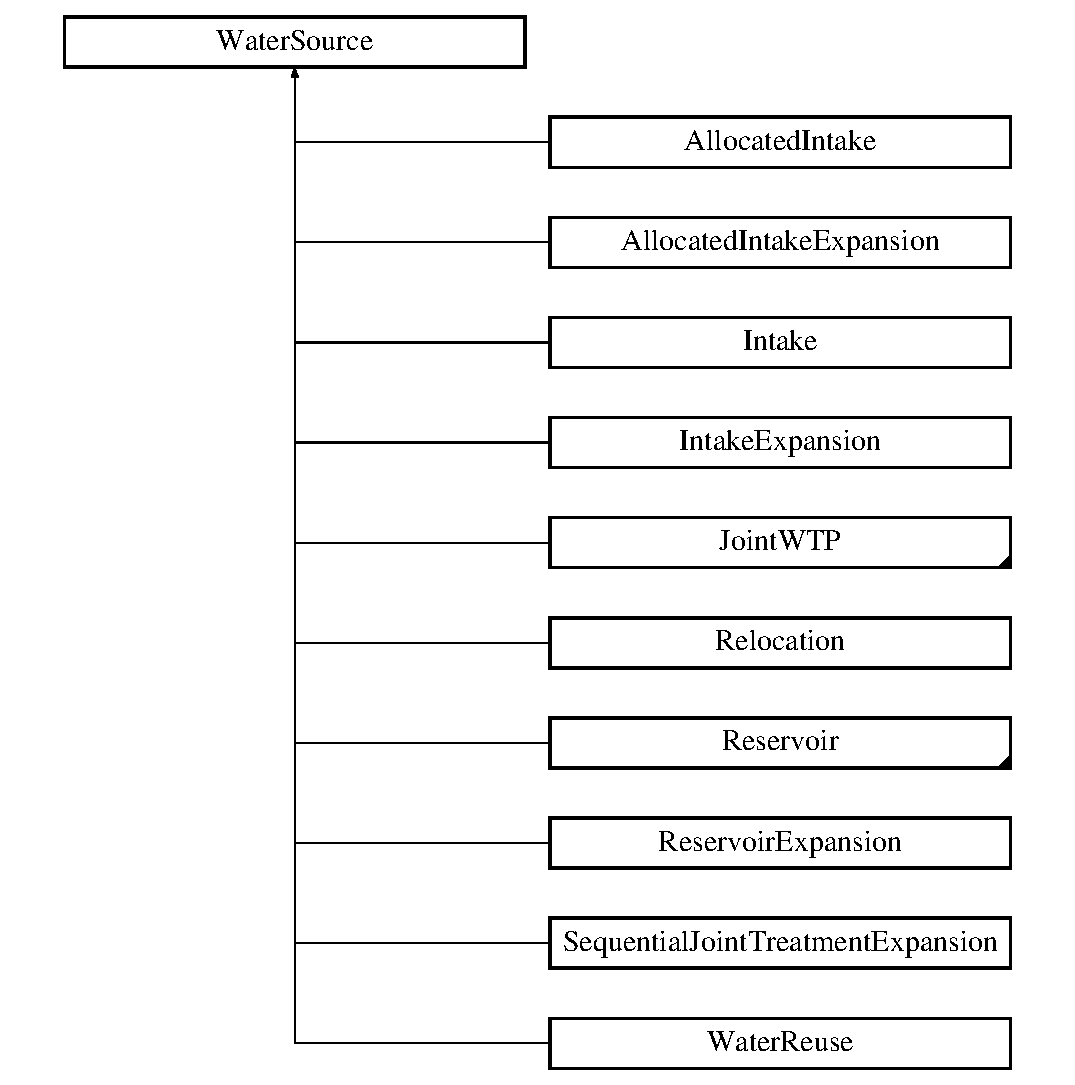
\includegraphics[height=11.000000cm]{classWaterSource}
\end{center}
\end{figure}
\subsection*{Public Member Functions}
\begin{DoxyCompactItemize}
\item 
\mbox{\hyperlink{classWaterSource_a27b9d29d6cbb36d128f740f7ca00f500}{Water\+Source}} (const char $\ast$\mbox{\hyperlink{classWaterSource_a846ea74c5b453d014f594d41fee8c765}{name}}, const int \mbox{\hyperlink{classWaterSource_a6eafe5dfefd317877d1244e8a7c6e742}{id}}, const vector$<$ \mbox{\hyperlink{classCatchment}{Catchment}} $\ast$$>$ \&\mbox{\hyperlink{classWaterSource_a8c18c34f23f8a06685c1d12f462ed830}{catchments}}, const double \mbox{\hyperlink{classWaterSource_a2ec257b415b248214a8bce7fc5267723}{capacity}}, vector$<$ int $>$ connected\+\_\+sources, double treatment\+\_\+capacity, const int \mbox{\hyperlink{classWaterSource_afdd12c29fc74ea21dff1f1be9b8c2b7b}{source\+\_\+type}})
\begin{DoxyCompactList}\small\item\em This constructor initializes a basic {\ttfamily \mbox{\hyperlink{classWaterSource}{Water\+Source}}} object with the given parameters. Used when the water source is built and operational. \end{DoxyCompactList}\item 
\mbox{\hyperlink{classWaterSource_a7723d343a0b8edff36018ca7acf09f62}{Water\+Source}} (const char $\ast$\mbox{\hyperlink{classWaterSource_a846ea74c5b453d014f594d41fee8c765}{name}}, const int \mbox{\hyperlink{classWaterSource_a6eafe5dfefd317877d1244e8a7c6e742}{id}}, const vector$<$ \mbox{\hyperlink{classCatchment}{Catchment}} $\ast$$>$ \&\mbox{\hyperlink{classWaterSource_a8c18c34f23f8a06685c1d12f462ed830}{catchments}}, const double \mbox{\hyperlink{classWaterSource_a2ec257b415b248214a8bce7fc5267723}{capacity}}, double treatment\+\_\+capacity, vector$<$ int $>$ connected\+\_\+sources, const int \mbox{\hyperlink{classWaterSource_afdd12c29fc74ea21dff1f1be9b8c2b7b}{source\+\_\+type}}, vector$<$ double $>$ $\ast$\mbox{\hyperlink{classWaterSource_aa73fe10cfc6579b2fb79529e1dde5140}{allocated\+\_\+treatment\+\_\+fractions}}, vector$<$ double $>$ $\ast$\mbox{\hyperlink{classWaterSource_a2f6655a80c4847fe039987255d9d998c}{allocated\+\_\+fractions}}, vector$<$ int $>$ $\ast$\mbox{\hyperlink{classWaterSource_ac345583fc2d0f7e1db31ee40244d7ace}{utilities\+\_\+with\+\_\+allocations}})
\begin{DoxyCompactList}\small\item\em This constructor initializes a {\ttfamily \mbox{\hyperlink{classWaterSource}{Water\+Source}}} object with pre-\/set allocation fractions and connected source details. Used when a water source is built and operational. \end{DoxyCompactList}\item 
\mbox{\hyperlink{classWaterSource_a48641ff06b69505ab298f4f23e759a22}{Water\+Source}} (const char $\ast$\mbox{\hyperlink{classWaterSource_a846ea74c5b453d014f594d41fee8c765}{name}}, const int \mbox{\hyperlink{classWaterSource_a6eafe5dfefd317877d1244e8a7c6e742}{id}}, const vector$<$ \mbox{\hyperlink{classCatchment}{Catchment}} $\ast$$>$ \&\mbox{\hyperlink{classWaterSource_a8c18c34f23f8a06685c1d12f462ed830}{catchments}}, const double \mbox{\hyperlink{classWaterSource_a2ec257b415b248214a8bce7fc5267723}{capacity}}, double treatment\+\_\+capacity, vector$<$ int $>$ connected\+\_\+sources, const int \mbox{\hyperlink{classWaterSource_afdd12c29fc74ea21dff1f1be9b8c2b7b}{source\+\_\+type}}, const vector$<$ double $>$ construction\+\_\+time\+\_\+range, double permitting\+\_\+period, \mbox{\hyperlink{classBond}{Bond}} \&bond)
\begin{DoxyCompactList}\small\item\em This constructor initializes a {\ttfamily \mbox{\hyperlink{classWaterSource}{Water\+Source}}} object with the provided parameters, including construction and permitting details. Used when the water source does not exist in the beginning of the simulation for water sources financed by only one bond. \end{DoxyCompactList}\item 
\mbox{\hyperlink{classWaterSource_a284e207f074da6f485d41f65ac025cf1}{Water\+Source}} (const char $\ast$\mbox{\hyperlink{classWaterSource_a846ea74c5b453d014f594d41fee8c765}{name}}, const int \mbox{\hyperlink{classWaterSource_a6eafe5dfefd317877d1244e8a7c6e742}{id}}, const vector$<$ \mbox{\hyperlink{classCatchment}{Catchment}} $\ast$$>$ \&\mbox{\hyperlink{classWaterSource_a8c18c34f23f8a06685c1d12f462ed830}{catchments}}, const double \mbox{\hyperlink{classWaterSource_a2ec257b415b248214a8bce7fc5267723}{capacity}}, double treatment\+\_\+capacity, vector$<$ int $>$ connected\+\_\+sources, const int \mbox{\hyperlink{classWaterSource_afdd12c29fc74ea21dff1f1be9b8c2b7b}{source\+\_\+type}}, const vector$<$ double $>$ construction\+\_\+time\+\_\+range, double permitting\+\_\+period, vector$<$ \mbox{\hyperlink{classBond}{Bond}} $\ast$$>$ \mbox{\hyperlink{classWaterSource_a413b094e11bdce62f4d82e5bb9e4706e}{bonds}})
\begin{DoxyCompactList}\small\item\em This constructor initializes a {\ttfamily \mbox{\hyperlink{classWaterSource}{Water\+Source}}} object with comprehensive parameters, including multiple bonds, construction, and permitting details. Used when the water source does not exist in the beginning of the simulation for water sources financed by a series of bonds (shared water source). \end{DoxyCompactList}\item 
\mbox{\hyperlink{classWaterSource_ae8cf84e138983737e044bc1217858021}{Water\+Source}} (const char $\ast$\mbox{\hyperlink{classWaterSource_a846ea74c5b453d014f594d41fee8c765}{name}}, const int \mbox{\hyperlink{classWaterSource_a6eafe5dfefd317877d1244e8a7c6e742}{id}}, const vector$<$ \mbox{\hyperlink{classCatchment}{Catchment}} $\ast$$>$ \&\mbox{\hyperlink{classWaterSource_a8c18c34f23f8a06685c1d12f462ed830}{catchments}}, const double \mbox{\hyperlink{classWaterSource_a2ec257b415b248214a8bce7fc5267723}{capacity}}, double treatment\+\_\+capacity, vector$<$ int $>$ \mbox{\hyperlink{classWaterSource_a49f9da70a5080abe82160b1a0d194e60}{built\+\_\+in\+\_\+sequence}}, const int \mbox{\hyperlink{classWaterSource_afdd12c29fc74ea21dff1f1be9b8c2b7b}{source\+\_\+type}}, vector$<$ double $>$ $\ast$\mbox{\hyperlink{classWaterSource_aa73fe10cfc6579b2fb79529e1dde5140}{allocated\+\_\+treatment\+\_\+fractions}}, vector$<$ double $>$ $\ast$\mbox{\hyperlink{classWaterSource_a2f6655a80c4847fe039987255d9d998c}{allocated\+\_\+fractions}}, vector$<$ int $>$ $\ast$\mbox{\hyperlink{classWaterSource_ac345583fc2d0f7e1db31ee40244d7ace}{utilities\+\_\+with\+\_\+allocations}}, const vector$<$ double $>$ construction\+\_\+time\+\_\+range, double permitting\+\_\+period, \mbox{\hyperlink{classBond}{Bond}} \&bond)
\begin{DoxyCompactList}\small\item\em This constructor initializes a {\ttfamily \mbox{\hyperlink{classWaterSource}{Water\+Source}}} object with detailed allocation settings, construction time, and bond financing. Used when a non-\/shared water source with multiple stages does not exist in the beginning of the simulation but has a built-\/in sequence of stages (i.\+e. low/high). \end{DoxyCompactList}\item 
\mbox{\hyperlink{classWaterSource_af9377254ee532ee30eaed78953336b5f}{Water\+Source}} (const char $\ast$\mbox{\hyperlink{classWaterSource_a846ea74c5b453d014f594d41fee8c765}{name}}, const int \mbox{\hyperlink{classWaterSource_a6eafe5dfefd317877d1244e8a7c6e742}{id}}, const vector$<$ \mbox{\hyperlink{classCatchment}{Catchment}} $\ast$$>$ \&\mbox{\hyperlink{classWaterSource_a8c18c34f23f8a06685c1d12f462ed830}{catchments}}, const double \mbox{\hyperlink{classWaterSource_a2ec257b415b248214a8bce7fc5267723}{capacity}}, double treatment\+\_\+capacity, vector$<$ int $>$ connected\+\_\+sources, vector$<$ int $>$ $\ast$\mbox{\hyperlink{classWaterSource_ac345583fc2d0f7e1db31ee40244d7ace}{utilities\+\_\+with\+\_\+allocations}}, vector$<$ double $>$ $\ast$utility\+\_\+treatment\+\_\+allocations, const int \mbox{\hyperlink{classWaterSource_afdd12c29fc74ea21dff1f1be9b8c2b7b}{source\+\_\+type}}, const vector$<$ double $>$ construction\+\_\+time\+\_\+range, double permitting\+\_\+period, vector$<$ \mbox{\hyperlink{classBond}{Bond}} $\ast$$>$ \mbox{\hyperlink{classWaterSource_a413b094e11bdce62f4d82e5bb9e4706e}{bonds}})
\begin{DoxyCompactList}\small\item\em This constructor initializes a {\ttfamily \mbox{\hyperlink{classWaterSource}{Water\+Source}}} object with parameters for utility allocations, water quality, and bond financing. Used when a shared water source does not exist in the beginning of the simulation and is of class {\ttfamily \mbox{\hyperlink{classJointWTP}{Joint\+W\+TP}}} (uses only {\ttfamily utility\+\_\+treatment\+\_\+allocations}). \end{DoxyCompactList}\item 
\mbox{\hyperlink{classWaterSource_a5d02f9dc15b18572bbfa945aeec4dbb0}{Water\+Source}} (const char $\ast$\mbox{\hyperlink{classWaterSource_a846ea74c5b453d014f594d41fee8c765}{name}}, const int \mbox{\hyperlink{classWaterSource_a6eafe5dfefd317877d1244e8a7c6e742}{id}}, const vector$<$ \mbox{\hyperlink{classCatchment}{Catchment}} $\ast$$>$ \&\mbox{\hyperlink{classWaterSource_a8c18c34f23f8a06685c1d12f462ed830}{catchments}}, const double \mbox{\hyperlink{classWaterSource_a2ec257b415b248214a8bce7fc5267723}{capacity}}, double treatment\+\_\+capacity, vector$<$ int $>$ connected\+\_\+sources, vector$<$ int $>$ $\ast$\mbox{\hyperlink{classWaterSource_ac345583fc2d0f7e1db31ee40244d7ace}{utilities\+\_\+with\+\_\+allocations}}, vector$<$ double $>$ $\ast$utility\+\_\+supply\+\_\+allocations, vector$<$ double $>$ $\ast$utility\+\_\+treatment\+\_\+allocations, const int \mbox{\hyperlink{classWaterSource_afdd12c29fc74ea21dff1f1be9b8c2b7b}{source\+\_\+type}}, const vector$<$ double $>$ construction\+\_\+time\+\_\+range, double permitting\+\_\+period, vector$<$ \mbox{\hyperlink{classBond}{Bond}} $\ast$$>$ \mbox{\hyperlink{classWaterSource_a413b094e11bdce62f4d82e5bb9e4706e}{bonds}})
\begin{DoxyCompactList}\small\item\em This constructor initializes a {\ttfamily \mbox{\hyperlink{classWaterSource}{Water\+Source}}} object with comprehensive parameters, including utility supply and treatment allocations, water quality management, and bond financing. Used when a shared water source does not exist in the beginning of the simulation and is of class {\ttfamily \mbox{\hyperlink{classAllocatedIntake}{Allocated\+Intake}}} or {\ttfamily Expansion} (uses {\ttfamily utility\+\_\+supply\+\_\+allocations} and {\ttfamily utility\+\_\+treatment\+\_\+allocations}). \end{DoxyCompactList}\item 
\mbox{\hyperlink{classWaterSource_aaa3aba0a9709cc1432f85f443b033a65}{Water\+Source}} (const \mbox{\hyperlink{classWaterSource}{Water\+Source}} \&water\+\_\+source)
\begin{DoxyCompactList}\small\item\em Copy constructor. \end{DoxyCompactList}\item 
virtual \mbox{\hyperlink{classWaterSource_aa3b9261264152782c3115d2f563f1caf}{$\sim$\+Water\+Source}} ()
\begin{DoxyCompactList}\small\item\em Destructor for the {\ttfamily \mbox{\hyperlink{classWaterSource}{Water\+Source}}} class. \end{DoxyCompactList}\item 
\mbox{\hyperlink{classWaterSource}{Water\+Source}} \& \mbox{\hyperlink{classWaterSource_af10a33e286cf44b362984ff8d8053c91}{operator=}} (const \mbox{\hyperlink{classWaterSource}{Water\+Source}} \&water\+\_\+source)
\begin{DoxyCompactList}\small\item\em Assignment operator for the {\ttfamily \mbox{\hyperlink{classWaterSource}{Water\+Source}}} class. \end{DoxyCompactList}\item 
bool \mbox{\hyperlink{classWaterSource_accb044cc78f9a444ca18bf7283b5b596}{operator$<$}} (const \mbox{\hyperlink{classWaterSource}{Water\+Source}} $\ast$other)
\begin{DoxyCompactList}\small\item\em Less-\/than operator for comparing two {\ttfamily \mbox{\hyperlink{classWaterSource}{Water\+Source}}} objects by their {\ttfamily id}. \end{DoxyCompactList}\item 
bool \mbox{\hyperlink{classWaterSource_a9db800769891e1f49d74a78298f4dac1}{operator$>$}} (const \mbox{\hyperlink{classWaterSource}{Water\+Source}} $\ast$other)
\begin{DoxyCompactList}\small\item\em Greater-\/than operator for comparing two {\ttfamily \mbox{\hyperlink{classWaterSource}{Water\+Source}}} objects by their {\ttfamily id}. \end{DoxyCompactList}\item 
bool \mbox{\hyperlink{classWaterSource_af25e06ec954898f3392cb125d2f2c2ad}{operator==}} (const \mbox{\hyperlink{classWaterSource}{Water\+Source}} $\ast$other)
\begin{DoxyCompactList}\small\item\em Equality operator for comparing two {\ttfamily \mbox{\hyperlink{classWaterSource}{Water\+Source}}} objects by their {\ttfamily id}. \end{DoxyCompactList}\item 
void \mbox{\hyperlink{classWaterSource_a1137cd86f8d3f8a48ebec54282132993}{continuity\+Water\+Source}} (int week, double \mbox{\hyperlink{classWaterSource_a7a69b2e9b6030f1035e6cf44d2918ee5}{upstream\+\_\+source\+\_\+inflow}}, double \mbox{\hyperlink{classWaterSource_aeb5a2d2d83383a70ca20f3e94635a9c7}{wastewater\+\_\+inflow}}, vector$<$ double $>$ \&demand\+\_\+outflow)
\begin{DoxyCompactList}\small\item\em Manages the continuity of a water source by either applying continuity or bypassing it. \end{DoxyCompactList}\item 
virtual void \mbox{\hyperlink{classWaterSource_ac2bc1a09fce3a3201d62a73052b27b0b}{add\+Treatment\+Capacity}} (const double added\+\_\+treatment\+\_\+capacity, int utility\+\_\+id)
\begin{DoxyCompactList}\small\item\em Adds treatment capacity to the water source. \end{DoxyCompactList}\item 
virtual void \mbox{\hyperlink{classWaterSource_a4a4d948033c57feb8523bd7d5828c59b}{remove\+Water}} (int allocation\+\_\+id, double volume)
\begin{DoxyCompactList}\small\item\em Removes water from the water source and updates demand. \end{DoxyCompactList}\item 
virtual void \mbox{\hyperlink{classWaterSource_ab869abb3d3dde1875e933482bedc3ae3}{add\+Capacity}} (double \mbox{\hyperlink{classWaterSource_a2ec257b415b248214a8bce7fc5267723}{capacity}}, int utility\+\_\+id)
\begin{DoxyCompactList}\small\item\em Adds capacity to the water source. \end{DoxyCompactList}\item 
virtual void \mbox{\hyperlink{classWaterSource_aaa55dc6e14ff184380300147b53c56ec}{set\+Online}} ()
\begin{DoxyCompactList}\small\item\em Sets the water source to be online. \end{DoxyCompactList}\item 
virtual bool \mbox{\hyperlink{classWaterSource_ad8496aea2d4ff97c8069b61cc984c799}{skip\+Construction}} (int utility\+\_\+id) const
\begin{DoxyCompactList}\small\item\em Determines whether the construction of the water source should be skipped. \end{DoxyCompactList}\item 
virtual double \mbox{\hyperlink{classWaterSource_ad4667296dc6b6dabc36b871529ca2749}{get\+Available\+Allocated\+Volume}} (int utility\+\_\+id)
\begin{DoxyCompactList}\small\item\em Retrieves the available allocated volume for a specific utility. \end{DoxyCompactList}\item 
virtual double \mbox{\hyperlink{classWaterSource_acb9e57253157c969fa57fc6e7b35ab68}{get\+Available\+Volume}} () const
\begin{DoxyCompactList}\small\item\em Retrieves the available volume of the water source. \end{DoxyCompactList}\item 
virtual void \mbox{\hyperlink{classWaterSource_a86999f23ec7f4fb518adb88e16f156a7}{set\+Full}} ()
\begin{DoxyCompactList}\small\item\em Sets the water source to its full capacity. \end{DoxyCompactList}\item 
virtual double \mbox{\hyperlink{classWaterSource_aeefcddb0119d5aab95dab03912a65cad}{get\+Supply\+Capacity}} ()
\begin{DoxyCompactList}\small\item\em Retrieves the available supply capacity of the water source. \end{DoxyCompactList}\item 
double \mbox{\hyperlink{classWaterSource_af7607924825ffe293179b09fe1bc466e}{get\+Min\+\_\+environmental\+\_\+outflow}} () const
\begin{DoxyCompactList}\small\item\em Retrieves the minimum environmental outflow for the water source. \end{DoxyCompactList}\item 
void \mbox{\hyperlink{classWaterSource_a406246432d29f49189d53207ab1d895a}{set\+Min\+\_\+environmental\+\_\+outflow}} (double \mbox{\hyperlink{classWaterSource_adae67ac96597e4b25332002b88a9a52b}{min\+\_\+environmental\+\_\+outflow}})
\begin{DoxyCompactList}\small\item\em Sets the minimum environmental outflow for the water source. \end{DoxyCompactList}\item 
const vector$<$ int $>$ \& \mbox{\hyperlink{classWaterSource_a1e28dee97f62fbb9845300fc2768d172}{get\+Built\+\_\+in\+\_\+sequence}} () const
\begin{DoxyCompactList}\small\item\em Gets the sequence (vector) of water sources to be built consecutively. \end{DoxyCompactList}\item 
double \mbox{\hyperlink{classWaterSource_a7678e05e3e73b927c0b47e3041d7415f}{get\+Total\+\_\+outflow}} () const
\begin{DoxyCompactList}\small\item\em Retrieves the total outflow from the water source. \end{DoxyCompactList}\item 
bool \mbox{\hyperlink{classWaterSource_a130fd661ff31c53115cca23e4e2f210a}{is\+Online}} () const
\begin{DoxyCompactList}\small\item\em Checks if the water source is online. \end{DoxyCompactList}\item 
void \mbox{\hyperlink{classWaterSource_ab53d376a425b8db603382ba27b52b1d4}{set\+Outflow\+\_\+previous\+\_\+week}} (double outflow\+\_\+previous\+\_\+week)
\begin{DoxyCompactList}\small\item\em Sets the total outflow for the previous week. \end{DoxyCompactList}\item 
double \mbox{\hyperlink{classWaterSource_ad7e60efd7395f8d3e674e602226e5ac1}{get\+Upstream\+\_\+source\+\_\+inflow}} () const
\begin{DoxyCompactList}\small\item\em Retrieves the upstream source inflow. \end{DoxyCompactList}\item 
double \mbox{\hyperlink{classWaterSource_ac57d6b292490333b5bc14233bce326ce}{get\+Demand}} () const
\begin{DoxyCompactList}\small\item\em Retrieves the total demand for the water source. \end{DoxyCompactList}\item 
double \mbox{\hyperlink{classWaterSource_afd2a153ba8f4ecaa9f8fa851d5a1727c}{get\+Upstream\+Catchment\+Inflow}} () const
\begin{DoxyCompactList}\small\item\em Retrieves the upstream catchment inflow. \end{DoxyCompactList}\item 
virtual void \mbox{\hyperlink{classWaterSource_a634904c510b16de6d7c057fed6d6e625}{set\+Realization}} (unsigned long r, vector$<$ double $>$ \&rdm\+\_\+factors)
\begin{DoxyCompactList}\small\item\em Sets the timeseries corresponding to the realization of the water source based on random factors. \end{DoxyCompactList}\item 
virtual double \mbox{\hyperlink{classWaterSource_ad218f2a603d7ebce268d800e0249a74c}{get\+Allocated\+Capacity}} (int utility\+\_\+id)
\begin{DoxyCompactList}\small\item\em Retrieves the allocated capacity of the water source. \end{DoxyCompactList}\item 
virtual double \mbox{\hyperlink{classWaterSource_acec9b1fef81a9b73c4517409438452ac}{get\+Allocated\+Fraction}} (int utility\+\_\+id)
\begin{DoxyCompactList}\small\item\em Retrieves the allocated fraction of the water source for a specific utility. \end{DoxyCompactList}\item 
double \mbox{\hyperlink{classWaterSource_a00b156a153fc24097e4c8a4e5c46c4e0}{get\+Evaporated\+\_\+volume}} () const
\begin{DoxyCompactList}\small\item\em Retrieves the total evaporated volume of the water source. \end{DoxyCompactList}\item 
virtual double \mbox{\hyperlink{classWaterSource_ab98528c4d2e6ecd14cb2c813b1d445c6}{get\+Allocated\+Treatment\+Capacity}} (int utility\+\_\+id) const
\begin{DoxyCompactList}\small\item\em Retrieves the allocated treatment capacity of the water source. \end{DoxyCompactList}\item 
double \mbox{\hyperlink{classWaterSource_a6228c9aee407ca2544753dbd2792c5fb}{get\+Total\+\_\+treatment\+\_\+capacity}} (int utility\+\_\+id) const
\begin{DoxyCompactList}\small\item\em Retrieves the total treatment capacity of the water source. \end{DoxyCompactList}\item 
void \mbox{\hyperlink{classWaterSource_ac834762e016e796968ad286feeca7be6}{set\+Allocations}} (vector$<$ int $>$ $\ast$\mbox{\hyperlink{classWaterSource_ac345583fc2d0f7e1db31ee40244d7ace}{utilities\+\_\+with\+\_\+allocations}}, vector$<$ double $>$ $\ast$\mbox{\hyperlink{classWaterSource_a2f6655a80c4847fe039987255d9d998c}{allocated\+\_\+fractions}}, vector$<$ double $>$ $\ast$\mbox{\hyperlink{classWaterSource_aa73fe10cfc6579b2fb79529e1dde5140}{allocated\+\_\+treatment\+\_\+fractions}})
\begin{DoxyCompactList}\small\item\em Sets the allocations for utilities in the water source. \end{DoxyCompactList}\item 
virtual void \mbox{\hyperlink{classWaterSource_afe2f6b96383abdb14563db279a261a31}{reset\+Allocations}} (const vector$<$ double $>$ $\ast$new\+\_\+allocated\+\_\+fractions)
\begin{DoxyCompactList}\small\item\em Resets the allocations for utilities in the water source. \end{DoxyCompactList}\item 
void \mbox{\hyperlink{classWaterSource_ae29ed4aa2b9c97c5a41772daf4631f05}{set\+Available\+Allocated\+Volumes}} (vector$<$ double $>$ \mbox{\hyperlink{classWaterSource_a77d3fe9ea445fc987b07debdfb9e2f5b}{available\+\_\+allocated\+\_\+volumes}}, double \mbox{\hyperlink{classWaterSource_a49e1a191152e344e2161e8db166e067a}{available\+\_\+volume}})
\begin{DoxyCompactList}\small\item\em Sets the available allocated volumes to each utility and available volume from the water source. \end{DoxyCompactList}\item 
vector$<$ double $>$ \mbox{\hyperlink{classWaterSource_a9a87dafd08834147bcf5004bc3907824}{get\+Available\+\_\+allocated\+\_\+volumes}} () const
\begin{DoxyCompactList}\small\item\em Returns the available allocated volumes for the water source. \end{DoxyCompactList}\item 
vector$<$ int $>$ $\ast$ \mbox{\hyperlink{classWaterSource_a41a9f1fb088f29633c9141687958c16e}{get\+Utilities\+\_\+with\+\_\+allocations}} () const
\begin{DoxyCompactList}\small\item\em Returns the I\+Ds of the utilities with allocations for the water source. \end{DoxyCompactList}\item 
double \mbox{\hyperlink{classWaterSource_aee22325e6af0e3c804ddbd9a3505be05}{get\+Wastewater\+\_\+inflow}} () const
\begin{DoxyCompactList}\small\item\em Returns the wastewater inflow to the water source. \end{DoxyCompactList}\item 
double \mbox{\hyperlink{classWaterSource_aa21d3f1c87ced40c2b673d9e43d99176}{get\+Permitting\+\_\+period}} () const
\begin{DoxyCompactList}\small\item\em Returns the permitting period of the water source. \end{DoxyCompactList}\item 
double \mbox{\hyperlink{classWaterSource_af6445a2dd3764907bcb9a37d4647f910}{get\+Available\+Supply\+Volume}} () const
\begin{DoxyCompactList}\small\item\em Returns the available supply volume of the water source. \end{DoxyCompactList}\item 
double \mbox{\hyperlink{classWaterSource_a63b1a410b47710db049e2b2e9c3c39a0}{get\+Allocated\+Inflow}} (int utility\+\_\+id) const
\begin{DoxyCompactList}\small\item\em This function returns the allocated inflow for a given utility. \end{DoxyCompactList}\item 
virtual double \mbox{\hyperlink{classWaterSource_a484bca192a9e3aacaad47db0afb8fbdd}{get\+Supply\+Allocated\+Fraction}} (int utility\+\_\+id)
\begin{DoxyCompactList}\small\item\em This function returns the supply allocated fraction for a given utility. \end{DoxyCompactList}\item 
virtual \mbox{\hyperlink{classBond}{Bond}} \& \mbox{\hyperlink{classWaterSource_acacef71453819480c5438ae5b433e66b}{get\+Bond}} (int utility\+\_\+id)
\begin{DoxyCompactList}\small\item\em This function returns the bond associated with a given utility ID. \end{DoxyCompactList}\item 
void \mbox{\hyperlink{classWaterSource_a47bc2006a1ef6ea4429d56a24319940f}{check\+For\+Input\+Errors\+Construction}} ()
\begin{DoxyCompactList}\small\item\em This function checks for input errors related to the permitting and construction times for a water source. \end{DoxyCompactList}\item 
int \mbox{\hyperlink{classWaterSource_aebc6985952d3e69f0d8ae1d0498a1ffe}{random\+Construction\+Time}} (double t0, double tf)
\begin{DoxyCompactList}\small\item\em This function generates a random construction time between the specified time bounds, converted to weeks. \end{DoxyCompactList}\item 
const double \mbox{\hyperlink{classWaterSource_ac1e8880f0aeb56b2728e253d3500ef40}{get\+Construction\+\_\+time}} () const
\begin{DoxyCompactList}\small\item\em This function returns the construction time of the water source. \end{DoxyCompactList}\item 
virtual double \mbox{\hyperlink{classWaterSource_a00a432eba75eaae7195338a8514ac853}{get\+Priority\+Source\+Potential\+Volume}} (int utility\+\_\+id) const
\begin{DoxyCompactList}\small\item\em This function returns the potential volume of the priority source for a given utility. \end{DoxyCompactList}\item 
virtual int \mbox{\hyperlink{classWaterSource_add1082429d114b41cb9e3afaa623aeb1}{get\+Agreement\+Type}} () const
\begin{DoxyCompactList}\small\item\em This function retrieves the agreement type of the water source. \end{DoxyCompactList}\item 
virtual int \mbox{\hyperlink{classWaterSource_a506c77317ae84db0a4d9ea2cd74ddb11}{get\+Parent\+Water\+Source\+ID}} () const
\begin{DoxyCompactList}\small\item\em This function retrieves the parent water source ID. \end{DoxyCompactList}\item 
void \mbox{\hyperlink{classWaterSource_adfc85c196cfc262d4b463e87c459eb3f}{reset\+Treatment\+Allocations}} (const vector$<$ double $>$ current\+\_\+treatment\+\_\+allocations, const vector$<$ double $>$ new\+\_\+treatment\+\_\+allocations)
\begin{DoxyCompactList}\small\item\em This function resets the treatment allocations for each utility based on the provided current and new treatment allocations. \end{DoxyCompactList}\item 
vector$<$ double $>$ \mbox{\hyperlink{classWaterSource_a48df9ae09a8a7844beb18c35382adba1}{get\+Allocated\+Treatment\+Capacities}} () const
\begin{DoxyCompactList}\small\item\em This function returns the vector of allocated treatment capacities to relevant utilities. \end{DoxyCompactList}\item 
void \mbox{\hyperlink{classWaterSource_abc7034b8c78e45d7b1fa4bd13b8a3bdd}{set\+Treatment\+Allocations}} (const vector$<$ double $>$ treatment\+\_\+capacity\+\_\+allocations)
\begin{DoxyCompactList}\small\item\em This function sets the treatment allocations for each utility based on the provided treatment capacity allocations. \end{DoxyCompactList}\item 
virtual double \mbox{\hyperlink{classWaterSource_ad943083d8b3bee60ad8d106bba8a5faa}{get\+Allocated\+Treatment\+Fraction}} (int utility\+\_\+id) const
\begin{DoxyCompactList}\small\item\em This function returns the allocated treatment fraction for a given utility. \end{DoxyCompactList}\item 
int \mbox{\hyperlink{classWaterSource_a9d85cbca88eefd54fda383237807470d}{get\+Water\+Quality\+Pool\+ID}} () const
\begin{DoxyCompactList}\small\item\em This function returns the water quality pool ID. \end{DoxyCompactList}\item 
vector$<$ double $>$ \mbox{\hyperlink{classWaterSource_a4b05ca30a659ff351e75c487f31ff847}{get\+Allocated\+Supply\+Capacities}} () const
\begin{DoxyCompactList}\small\item\em This function returns the vector of allocated supply capacities. \end{DoxyCompactList}\end{DoxyCompactItemize}
\subsection*{Static Public Member Functions}
\begin{DoxyCompactItemize}
\item 
static bool \mbox{\hyperlink{classWaterSource_a25d4ad4251b78267618b2f0ef5a501dc}{compare}} (\mbox{\hyperlink{classWaterSource}{Water\+Source}} $\ast$lhs, \mbox{\hyperlink{classWaterSource}{Water\+Source}} $\ast$rhs)
\begin{DoxyCompactList}\small\item\em Compares two water sources based on their ID. \end{DoxyCompactList}\item 
static void \mbox{\hyperlink{classWaterSource_a4c8f4c120b9101767b6013a78eb2c5d4}{set\+Seed}} (int \mbox{\hyperlink{classWaterSource_abaf6cb0ecca08c87428ad516f11f8c2e}{seed}})
\begin{DoxyCompactList}\small\item\em This function sets the seed value for the random number generator. \end{DoxyCompactList}\item 
static void \mbox{\hyperlink{classWaterSource_a04f94831f4816bb277c5a615eace7779}{unset\+Seed}} ()
\begin{DoxyCompactList}\small\item\em This function unsets the seed value for the random number generator. \end{DoxyCompactList}\end{DoxyCompactItemize}
\subsection*{Public Attributes}
\begin{DoxyCompactItemize}
\item 
const int \mbox{\hyperlink{classWaterSource_a6eafe5dfefd317877d1244e8a7c6e742}{id}}
\begin{DoxyCompactList}\small\item\em The unique identifier of the water source. \end{DoxyCompactList}\item 
const char $\ast$ \mbox{\hyperlink{classWaterSource_a846ea74c5b453d014f594d41fee8c765}{name}}
\begin{DoxyCompactList}\small\item\em The name of the water source. \end{DoxyCompactList}\item 
const int \mbox{\hyperlink{classWaterSource_afdd12c29fc74ea21dff1f1be9b8c2b7b}{source\+\_\+type}}
\begin{DoxyCompactList}\small\item\em The type of the water source. \end{DoxyCompactList}\item 
const double \mbox{\hyperlink{classWaterSource_ae059fbe3f911a819bac0202f7f45e8e4}{construction\+\_\+time}}
\begin{DoxyCompactList}\small\item\em The time required to build the water source. \end{DoxyCompactList}\end{DoxyCompactItemize}
\subsection*{Protected Member Functions}
\begin{DoxyCompactItemize}
\item 
virtual void \mbox{\hyperlink{classWaterSource_ac070445379fe706f65b977dade4f3fbc}{apply\+Continuity}} (int week, double \mbox{\hyperlink{classWaterSource_a7a69b2e9b6030f1035e6cf44d2918ee5}{upstream\+\_\+source\+\_\+inflow}}, double \mbox{\hyperlink{classWaterSource_aeb5a2d2d83383a70ca20f3e94635a9c7}{wastewater\+\_\+inflow}}, vector$<$ double $>$ \&demand\+\_\+outflow)=0
\begin{DoxyCompactList}\small\item\em This function handles the continuity calculations for a water source, ensuring proper inflow and outflow. \end{DoxyCompactList}\item 
void \mbox{\hyperlink{classWaterSource_abeb8ba4b51c2b270baf9162df76d8b58}{bypass}} (int week, double total\+\_\+upstream\+\_\+inflow)
\begin{DoxyCompactList}\small\item\em This function bypasses continuity calculations, routing all inflows downstream without adjustments. Does not apply continuity to the water source, by instead just treats it as non existing, i.\+e. outflow = inflow + catchment\+\_\+flow. \end{DoxyCompactList}\end{DoxyCompactItemize}
\subsection*{Protected Attributes}
\begin{DoxyCompactItemize}
\item 
double \mbox{\hyperlink{classWaterSource_a49e1a191152e344e2161e8db166e067a}{available\+\_\+volume}} = 0
\begin{DoxyCompactList}\small\item\em Total available volume in the water source. \end{DoxyCompactList}\item 
double \mbox{\hyperlink{classWaterSource_a5e6992931464ed75576326b9f1bd3c4f}{total\+\_\+outflow}} = 0
\begin{DoxyCompactList}\small\item\em Total outflow from the water source. \end{DoxyCompactList}\item 
double \mbox{\hyperlink{classWaterSource_a7a69b2e9b6030f1035e6cf44d2918ee5}{upstream\+\_\+source\+\_\+inflow}} = 0
\begin{DoxyCompactList}\small\item\em Total upstream inflow to the water source. \end{DoxyCompactList}\item 
double \mbox{\hyperlink{classWaterSource_aeb5a2d2d83383a70ca20f3e94635a9c7}{wastewater\+\_\+inflow}} = 0
\begin{DoxyCompactList}\small\item\em Total inflow from wastewater treatment plants. \end{DoxyCompactList}\item 
double \mbox{\hyperlink{classWaterSource_aceb2d77612db7ba71a171848a5e03b4f}{upstream\+\_\+catchment\+\_\+inflow}} = 0
\begin{DoxyCompactList}\small\item\em Total inflow from upstream catchments into the water source. \end{DoxyCompactList}\item 
double \mbox{\hyperlink{classWaterSource_a1934917dd35a2508a5102eb5831431b7}{total\+\_\+demand}} = 0
\begin{DoxyCompactList}\small\item\em Total demand being drawn from the water source. \end{DoxyCompactList}\item 
double \mbox{\hyperlink{classWaterSource_a3f04ae75d6235117d391dece2d323890}{policy\+\_\+added\+\_\+demand}} = 0
\begin{DoxyCompactList}\small\item\em The total demand added to the water source by policy. F\+I\+X\+ME\+: Definition is not clear. \end{DoxyCompactList}\item 
double \mbox{\hyperlink{classWaterSource_a036d7980e74224fd5f5c6a390e0d5abb}{permitting\+\_\+time}} = N\+O\+N\+\_\+\+I\+N\+I\+T\+I\+A\+L\+I\+Z\+ED
\begin{DoxyCompactList}\small\item\em Permitting time required to build the water source. \end{DoxyCompactList}\item 
vector$<$ \mbox{\hyperlink{classBond}{Bond}} $\ast$ $>$ \mbox{\hyperlink{classWaterSource_a413b094e11bdce62f4d82e5bb9e4706e}{bonds}}
\begin{DoxyCompactList}\small\item\em Bonds associated with the water source. \end{DoxyCompactList}\item 
double \mbox{\hyperlink{classWaterSource_a67165e29345b61f36c8d8ccf3f648819}{upstream\+\_\+min\+\_\+env\+\_\+inflow}} = 0
\begin{DoxyCompactList}\small\item\em Minimum upstream environmental inflow required by the water source. \end{DoxyCompactList}\item 
double \mbox{\hyperlink{classWaterSource_a2ec257b415b248214a8bce7fc5267723}{capacity}} = N\+O\+N\+\_\+\+I\+N\+I\+T\+I\+A\+L\+I\+Z\+ED
\begin{DoxyCompactList}\small\item\em Total capacity of the water source. \end{DoxyCompactList}\item 
vector$<$ int $>$ \mbox{\hyperlink{classWaterSource_a49f9da70a5080abe82160b1a0d194e60}{built\+\_\+in\+\_\+sequence}}
\begin{DoxyCompactList}\small\item\em Sequence of water sources that are connected to this water source. F\+I\+X\+ME\+: Needs to be clarified. \end{DoxyCompactList}\item 
vector$<$ double $>$ \mbox{\hyperlink{classWaterSource_a77d3fe9ea445fc987b07debdfb9e2f5b}{available\+\_\+allocated\+\_\+volumes}}
\begin{DoxyCompactList}\small\item\em Available allocated volumes of raw water supplying the water source. \end{DoxyCompactList}\item 
vector$<$ double $>$ \mbox{\hyperlink{classWaterSource_ab94063d51314cfb896010408ae32fa9c}{allocated\+\_\+capacities}}
\begin{DoxyCompactList}\small\item\em Allocated capacities of the water source to each utility. \end{DoxyCompactList}\item 
vector$<$ double $>$ \mbox{\hyperlink{classWaterSource_a87dc0bfb5cf4e2b9a953c7a80058c923}{allocated\+\_\+treatment\+\_\+capacities}}
\begin{DoxyCompactList}\small\item\em Allocated treatment capacities of the water source to each utility. \end{DoxyCompactList}\item 
vector$<$ double $>$ \mbox{\hyperlink{classWaterSource_aa73fe10cfc6579b2fb79529e1dde5140}{allocated\+\_\+treatment\+\_\+fractions}}
\begin{DoxyCompactList}\small\item\em Allocated treatment fractions of the water source to each utility. \end{DoxyCompactList}\item 
vector$<$ double $>$ \mbox{\hyperlink{classWaterSource_a2f6655a80c4847fe039987255d9d998c}{allocated\+\_\+fractions}}
\begin{DoxyCompactList}\small\item\em Allocated overall fractions of the water source to each utility. \end{DoxyCompactList}\item 
vector$<$ double $>$ \mbox{\hyperlink{classWaterSource_a87535be59994b2602576cdf34dbe04b9}{supply\+\_\+allocated\+\_\+fractions}}
\begin{DoxyCompactList}\small\item\em Utilities with allocations to the water source. \end{DoxyCompactList}\item 
vector$<$ int $>$ $\ast$ \mbox{\hyperlink{classWaterSource_ac345583fc2d0f7e1db31ee40244d7ace}{utilities\+\_\+with\+\_\+allocations}} = nullptr
\begin{DoxyCompactList}\small\item\em Utilities with allocations to the water source. \end{DoxyCompactList}\item 
int \mbox{\hyperlink{classWaterSource_acef73d9b1675fb6db9ec39347514db6d}{wq\+\_\+pool\+\_\+id}} = N\+O\+N\+\_\+\+I\+N\+I\+T\+I\+A\+L\+I\+Z\+ED
\begin{DoxyCompactList}\small\item\em ID of the water quality pool, which is the water source used to ensure minimum environmental flows downstream. \end{DoxyCompactList}\item 
double \mbox{\hyperlink{classWaterSource_a4be6864dc196287bdf8329b3aa6ca662}{total\+\_\+allocated\+\_\+fraction}} = N\+O\+N\+\_\+\+I\+N\+I\+T\+I\+A\+L\+I\+Z\+ED
\begin{DoxyCompactList}\small\item\em Total allocated fraction of the catchments supplying the water source. \end{DoxyCompactList}\item 
bool \mbox{\hyperlink{classWaterSource_aef4e289b47c2360f2e991ea3ee535781}{online}}
\begin{DoxyCompactList}\small\item\em Flag indicating if the water source is online. \end{DoxyCompactList}\item 
vector$<$ \mbox{\hyperlink{classCatchment}{Catchment}} $>$ \mbox{\hyperlink{classWaterSource_a8c18c34f23f8a06685c1d12f462ed830}{catchments}}
\begin{DoxyCompactList}\small\item\em A vector of all the catchements that supply the water source. \end{DoxyCompactList}\item 
double \mbox{\hyperlink{classWaterSource_adae67ac96597e4b25332002b88a9a52b}{min\+\_\+environmental\+\_\+outflow}} = 0
\begin{DoxyCompactList}\small\item\em Minimum environmental outflow required by the water source. \end{DoxyCompactList}\item 
double \mbox{\hyperlink{classWaterSource_a6085899c4b4cc40fa80784203e1a9755}{evaporated\+\_\+volume}} = 0
\begin{DoxyCompactList}\small\item\em Total volume evaporated from the water source. \end{DoxyCompactList}\item 
double \mbox{\hyperlink{classWaterSource_a2fdfd5ff7d103e71108cf2a31babaccb}{total\+\_\+treatment\+\_\+capacity}} = 0
\begin{DoxyCompactList}\small\item\em Total treatment capacity of the water source. \end{DoxyCompactList}\item 
int \mbox{\hyperlink{classWaterSource_a83c6dcf19b64533ce4bc3b918ce6cc8e}{highest\+\_\+alloc\+\_\+id}} = N\+O\+N\+\_\+\+I\+N\+I\+T\+I\+A\+L\+I\+Z\+ED
\begin{DoxyCompactList}\small\item\em The ID of the utility with the highest percent allocation from the water source. \end{DoxyCompactList}\end{DoxyCompactItemize}
\subsection*{Static Protected Attributes}
\begin{DoxyCompactItemize}
\item 
static int \mbox{\hyperlink{classWaterSource_abaf6cb0ecca08c87428ad516f11f8c2e}{seed}}
\begin{DoxyCompactList}\small\item\em Seed to generate the random construction time. F\+I\+X\+ME\+: Needs to be clarified. \end{DoxyCompactList}\end{DoxyCompactItemize}


\subsection{Constructor \& Destructor Documentation}
\mbox{\Hypertarget{classWaterSource_a27b9d29d6cbb36d128f740f7ca00f500}\label{classWaterSource_a27b9d29d6cbb36d128f740f7ca00f500}} 
\index{Water\+Source@{Water\+Source}!Water\+Source@{Water\+Source}}
\index{Water\+Source@{Water\+Source}!Water\+Source@{Water\+Source}}
\subsubsection{\texorpdfstring{Water\+Source()}{WaterSource()}\hspace{0.1cm}{\footnotesize\ttfamily [1/8]}}
{\footnotesize\ttfamily Water\+Source\+::\+Water\+Source (\begin{DoxyParamCaption}\item[{const char $\ast$}]{name,  }\item[{const int}]{id,  }\item[{const vector$<$ \mbox{\hyperlink{classCatchment}{Catchment}} $\ast$$>$ \&}]{catchments,  }\item[{const double}]{capacity,  }\item[{vector$<$ int $>$}]{connected\+\_\+sources,  }\item[{double}]{treatment\+\_\+capacity,  }\item[{const int}]{source\+\_\+type }\end{DoxyParamCaption})}



This constructor initializes a basic {\ttfamily \mbox{\hyperlink{classWaterSource}{Water\+Source}}} object with the given parameters. Used when the water source is built and operational. 


\begin{DoxyParams}{Parameters}
{\em name} & The name of the water source. \\
\hline
{\em id} & The unique identifier for the water source. \\
\hline
{\em catchments} & A vector of pointers to {\ttfamily \mbox{\hyperlink{classCatchment}{Catchment}}} objects supplying this water source. \\
\hline
{\em capacity} & The total storage capacity of the water source. \\
\hline
{\em connected\+\_\+sources} & A vector of I\+Ds representing sources connected to this water source. \\
\hline
{\em treatment\+\_\+capacity} & The total treatment capacity of the water source. \\
\hline
{\em source\+\_\+type} & The type of water source (e.\+g., reservoir, river, etc.).\\
\hline
\end{DoxyParams}
\begin{DoxyReturn}{Returns}
A new {\ttfamily \mbox{\hyperlink{classWaterSource}{Water\+Source}}} object. 
\end{DoxyReturn}
\mbox{\Hypertarget{classWaterSource_a7723d343a0b8edff36018ca7acf09f62}\label{classWaterSource_a7723d343a0b8edff36018ca7acf09f62}} 
\index{Water\+Source@{Water\+Source}!Water\+Source@{Water\+Source}}
\index{Water\+Source@{Water\+Source}!Water\+Source@{Water\+Source}}
\subsubsection{\texorpdfstring{Water\+Source()}{WaterSource()}\hspace{0.1cm}{\footnotesize\ttfamily [2/8]}}
{\footnotesize\ttfamily Water\+Source\+::\+Water\+Source (\begin{DoxyParamCaption}\item[{const char $\ast$}]{name,  }\item[{const int}]{id,  }\item[{const vector$<$ \mbox{\hyperlink{classCatchment}{Catchment}} $\ast$$>$ \&}]{catchments,  }\item[{const double}]{capacity,  }\item[{double}]{treatment\+\_\+capacity,  }\item[{vector$<$ int $>$}]{connected\+\_\+sources,  }\item[{const int}]{source\+\_\+type,  }\item[{vector$<$ double $>$ $\ast$}]{allocated\+\_\+treatment\+\_\+fractions,  }\item[{vector$<$ double $>$ $\ast$}]{allocated\+\_\+fractions,  }\item[{vector$<$ int $>$ $\ast$}]{utilities\+\_\+with\+\_\+allocations }\end{DoxyParamCaption})}



This constructor initializes a {\ttfamily \mbox{\hyperlink{classWaterSource}{Water\+Source}}} object with pre-\/set allocation fractions and connected source details. Used when a water source is built and operational. 


\begin{DoxyParams}{Parameters}
{\em name} & The name of the water source. \\
\hline
{\em id} & The unique identifier for the water source. \\
\hline
{\em catchments} & A vector of pointers to {\ttfamily \mbox{\hyperlink{classCatchment}{Catchment}}} objects associated with this water source. \\
\hline
{\em capacity} & The total storage capacity of the water source (in cubic meters). \\
\hline
{\em treatment\+\_\+capacity} & The total treatment capacity of the water source (in cubic meters per week). \\
\hline
{\em connected\+\_\+sources} & A vector of I\+Ds representing sources connected to this water source. \\
\hline
{\em source\+\_\+type} & The type of water source (e.\+g., reservoir, river, etc.). \\
\hline
{\em allocated\+\_\+treatment\+\_\+fractions} & A pointer to a vector of pre-\/set fractions of the total treatment capacity allocated to utilities. \\
\hline
{\em allocated\+\_\+fractions} & A pointer to a vector of pre-\/set fractions of the total storage capacity allocated to utilities. \\
\hline
{\em utilities\+\_\+with\+\_\+allocations} & A pointer to a vector of I\+Ds for utilities allocated to this water source.\\
\hline
\end{DoxyParams}
\begin{DoxyReturn}{Returns}
A new {\ttfamily \mbox{\hyperlink{classWaterSource}{Water\+Source}}} object.
\end{DoxyReturn}

\begin{DoxyExceptions}{Exceptions}
{\em std\+::runtime\+\_\+error} & if any issues arise in setting allocations (handled by {\ttfamily set\+Allocations}). \\
\hline
\end{DoxyExceptions}
\mbox{\Hypertarget{classWaterSource_a48641ff06b69505ab298f4f23e759a22}\label{classWaterSource_a48641ff06b69505ab298f4f23e759a22}} 
\index{Water\+Source@{Water\+Source}!Water\+Source@{Water\+Source}}
\index{Water\+Source@{Water\+Source}!Water\+Source@{Water\+Source}}
\subsubsection{\texorpdfstring{Water\+Source()}{WaterSource()}\hspace{0.1cm}{\footnotesize\ttfamily [3/8]}}
{\footnotesize\ttfamily Water\+Source\+::\+Water\+Source (\begin{DoxyParamCaption}\item[{const char $\ast$}]{name,  }\item[{const int}]{id,  }\item[{const vector$<$ \mbox{\hyperlink{classCatchment}{Catchment}} $\ast$$>$ \&}]{catchments,  }\item[{const double}]{capacity,  }\item[{double}]{treatment\+\_\+capacity,  }\item[{vector$<$ int $>$}]{connected\+\_\+sources,  }\item[{const int}]{source\+\_\+type,  }\item[{const vector$<$ double $>$}]{construction\+\_\+time\+\_\+range,  }\item[{double}]{permitting\+\_\+period,  }\item[{\mbox{\hyperlink{classBond}{Bond}} \&}]{bond }\end{DoxyParamCaption})}



This constructor initializes a {\ttfamily \mbox{\hyperlink{classWaterSource}{Water\+Source}}} object with the provided parameters, including construction and permitting details. Used when the water source does not exist in the beginning of the simulation for water sources financed by only one bond. 


\begin{DoxyParams}{Parameters}
{\em name} & The name of the water source. \\
\hline
{\em id} & The unique identifier for the water source. \\
\hline
{\em catchments} & A vector of pointers to {\ttfamily \mbox{\hyperlink{classCatchment}{Catchment}}} objects associated with this water source. \\
\hline
{\em capacity} & The total storage capacity of the water source. \\
\hline
{\em treatment\+\_\+capacity} & The total treatment capacity of the water source. \\
\hline
{\em connected\+\_\+sources} & A vector of I\+Ds representing sources connected to this water source. \\
\hline
{\em source\+\_\+type} & The type of water source (e.\+g., reservoir, river, etc.). \\
\hline
{\em construction\+\_\+time\+\_\+range} & A vector containing the minimum and maximum construction time range. \\
\hline
{\em permitting\+\_\+period} & The permitting time required for the water source. \\
\hline
{\em bond} & A reference to a {\ttfamily \mbox{\hyperlink{classBond}{Bond}}} object associated with financing this water source.\\
\hline
\end{DoxyParams}
\begin{DoxyReturn}{Returns}
A new {\ttfamily \mbox{\hyperlink{classWaterSource}{Water\+Source}}} object.
\end{DoxyReturn}

\begin{DoxyExceptions}{Exceptions}
{\em std\+::invalid\+\_\+argument} & if permitting or construction time is NaN or negative (checked by {\ttfamily check\+For\+Input\+Errors\+Construction}). \\
\hline
\end{DoxyExceptions}
\mbox{\Hypertarget{classWaterSource_a284e207f074da6f485d41f65ac025cf1}\label{classWaterSource_a284e207f074da6f485d41f65ac025cf1}} 
\index{Water\+Source@{Water\+Source}!Water\+Source@{Water\+Source}}
\index{Water\+Source@{Water\+Source}!Water\+Source@{Water\+Source}}
\subsubsection{\texorpdfstring{Water\+Source()}{WaterSource()}\hspace{0.1cm}{\footnotesize\ttfamily [4/8]}}
{\footnotesize\ttfamily Water\+Source\+::\+Water\+Source (\begin{DoxyParamCaption}\item[{const char $\ast$}]{name,  }\item[{const int}]{id,  }\item[{const vector$<$ \mbox{\hyperlink{classCatchment}{Catchment}} $\ast$$>$ \&}]{catchments,  }\item[{const double}]{capacity,  }\item[{double}]{treatment\+\_\+capacity,  }\item[{vector$<$ int $>$}]{connected\+\_\+sources,  }\item[{const int}]{source\+\_\+type,  }\item[{const vector$<$ double $>$}]{construction\+\_\+time\+\_\+range,  }\item[{double}]{permitting\+\_\+period,  }\item[{vector$<$ \mbox{\hyperlink{classBond}{Bond}} $\ast$$>$}]{bonds }\end{DoxyParamCaption})}



This constructor initializes a {\ttfamily \mbox{\hyperlink{classWaterSource}{Water\+Source}}} object with comprehensive parameters, including multiple bonds, construction, and permitting details. Used when the water source does not exist in the beginning of the simulation for water sources financed by a series of bonds (shared water source). 


\begin{DoxyParams}{Parameters}
{\em name} & The name of the water source. \\
\hline
{\em id} & The unique identifier for the water source. \\
\hline
{\em catchments} & A vector of pointers to {\ttfamily \mbox{\hyperlink{classCatchment}{Catchment}}} objects associated with this water source. \\
\hline
{\em capacity} & The total storage capacity of the water source. \\
\hline
{\em treatment\+\_\+capacity} & The total treatment capacity of the water source. \\
\hline
{\em connected\+\_\+sources} & A vector of I\+Ds representing sources connected to this water source. \\
\hline
{\em source\+\_\+type} & The type of water source (e.\+g., reservoir, river, etc.). \\
\hline
{\em construction\+\_\+time\+\_\+range} & A vector containing the minimum and maximum construction time range. \\
\hline
{\em permitting\+\_\+period} & The permitting time required for the water source. \\
\hline
{\em bonds} & A vector of pointers to {\ttfamily \mbox{\hyperlink{classBond}{Bond}}} objects associated with financing this water source.\\
\hline
\end{DoxyParams}
\begin{DoxyReturn}{Returns}
A new {\ttfamily \mbox{\hyperlink{classWaterSource}{Water\+Source}}} object.
\end{DoxyReturn}

\begin{DoxyExceptions}{Exceptions}
{\em std\+::invalid\+\_\+argument} & if permitting or construction time is NaN or negative (checked by {\ttfamily check\+For\+Input\+Errors\+Construction}). \\
\hline
\end{DoxyExceptions}
\mbox{\Hypertarget{classWaterSource_ae8cf84e138983737e044bc1217858021}\label{classWaterSource_ae8cf84e138983737e044bc1217858021}} 
\index{Water\+Source@{Water\+Source}!Water\+Source@{Water\+Source}}
\index{Water\+Source@{Water\+Source}!Water\+Source@{Water\+Source}}
\subsubsection{\texorpdfstring{Water\+Source()}{WaterSource()}\hspace{0.1cm}{\footnotesize\ttfamily [5/8]}}
{\footnotesize\ttfamily Water\+Source\+::\+Water\+Source (\begin{DoxyParamCaption}\item[{const char $\ast$}]{name,  }\item[{const int}]{id,  }\item[{const vector$<$ \mbox{\hyperlink{classCatchment}{Catchment}} $\ast$$>$ \&}]{catchments,  }\item[{const double}]{capacity,  }\item[{double}]{treatment\+\_\+capacity,  }\item[{vector$<$ int $>$}]{built\+\_\+in\+\_\+sequence,  }\item[{const int}]{source\+\_\+type,  }\item[{vector$<$ double $>$ $\ast$}]{allocated\+\_\+treatment\+\_\+fractions,  }\item[{vector$<$ double $>$ $\ast$}]{allocated\+\_\+fractions,  }\item[{vector$<$ int $>$ $\ast$}]{utilities\+\_\+with\+\_\+allocations,  }\item[{const vector$<$ double $>$}]{construction\+\_\+time\+\_\+range,  }\item[{double}]{permitting\+\_\+period,  }\item[{\mbox{\hyperlink{classBond}{Bond}} \&}]{bond }\end{DoxyParamCaption})}



This constructor initializes a {\ttfamily \mbox{\hyperlink{classWaterSource}{Water\+Source}}} object with detailed allocation settings, construction time, and bond financing. Used when a non-\/shared water source with multiple stages does not exist in the beginning of the simulation but has a built-\/in sequence of stages (i.\+e. low/high). 


\begin{DoxyParams}{Parameters}
{\em name} & The name of the water source. \\
\hline
{\em id} & The unique identifier for the water source. \\
\hline
{\em catchments} & A vector of pointers to {\ttfamily \mbox{\hyperlink{classCatchment}{Catchment}}} objects associated with this water source. \\
\hline
{\em capacity} & The total storage capacity of the water source (in cubic meters). \\
\hline
{\em treatment\+\_\+capacity} & The total treatment capacity of the water source (in cubic meters per week). \\
\hline
{\em built\+\_\+in\+\_\+sequence} & A vector of I\+Ds representing the construction sequence for this water source. \\
\hline
{\em source\+\_\+type} & The type of water source (e.\+g., reservoir, river, etc.). \\
\hline
{\em allocated\+\_\+treatment\+\_\+fractions} & A pointer to a vector of fractions of total treatment capacity allocated to utilities. \\
\hline
{\em allocated\+\_\+fractions} & A pointer to a vector of fractions of total storage capacity allocated to utilities. \\
\hline
{\em utilities\+\_\+with\+\_\+allocations} & A pointer to a vector of I\+Ds for utilities allocated to this water source. \\
\hline
{\em construction\+\_\+time\+\_\+range} & A vector containing the minimum and maximum construction time range (in years). \\
\hline
{\em permitting\+\_\+period} & The permitting time required for the water source (in years). \\
\hline
{\em bond} & A reference to a {\ttfamily \mbox{\hyperlink{classBond}{Bond}}} object representing financing details for this water source.\\
\hline
\end{DoxyParams}
\begin{DoxyReturn}{Returns}
A new {\ttfamily \mbox{\hyperlink{classWaterSource}{Water\+Source}}} object.
\end{DoxyReturn}

\begin{DoxyExceptions}{Exceptions}
{\em std\+::invalid\+\_\+argument} & if permitting or construction time is NaN or negative (checked by {\ttfamily check\+For\+Input\+Errors\+Construction}). \\
\hline
\end{DoxyExceptions}
\mbox{\Hypertarget{classWaterSource_af9377254ee532ee30eaed78953336b5f}\label{classWaterSource_af9377254ee532ee30eaed78953336b5f}} 
\index{Water\+Source@{Water\+Source}!Water\+Source@{Water\+Source}}
\index{Water\+Source@{Water\+Source}!Water\+Source@{Water\+Source}}
\subsubsection{\texorpdfstring{Water\+Source()}{WaterSource()}\hspace{0.1cm}{\footnotesize\ttfamily [6/8]}}
{\footnotesize\ttfamily Water\+Source\+::\+Water\+Source (\begin{DoxyParamCaption}\item[{const char $\ast$}]{name,  }\item[{const int}]{id,  }\item[{const vector$<$ \mbox{\hyperlink{classCatchment}{Catchment}} $\ast$$>$ \&}]{catchments,  }\item[{const double}]{capacity,  }\item[{double}]{treatment\+\_\+capacity,  }\item[{vector$<$ int $>$}]{connected\+\_\+sources,  }\item[{vector$<$ int $>$ $\ast$}]{utilities\+\_\+with\+\_\+allocations,  }\item[{vector$<$ double $>$ $\ast$}]{utility\+\_\+treatment\+\_\+allocations,  }\item[{const int}]{source\+\_\+type,  }\item[{const vector$<$ double $>$}]{construction\+\_\+time\+\_\+range,  }\item[{double}]{permitting\+\_\+period,  }\item[{vector$<$ \mbox{\hyperlink{classBond}{Bond}} $\ast$$>$}]{bonds }\end{DoxyParamCaption})}



This constructor initializes a {\ttfamily \mbox{\hyperlink{classWaterSource}{Water\+Source}}} object with parameters for utility allocations, water quality, and bond financing. Used when a shared water source does not exist in the beginning of the simulation and is of class {\ttfamily \mbox{\hyperlink{classJointWTP}{Joint\+W\+TP}}} (uses only {\ttfamily utility\+\_\+treatment\+\_\+allocations}). 


\begin{DoxyParams}{Parameters}
{\em name} & The name of the water source. \\
\hline
{\em id} & The unique identifier for the water source. \\
\hline
{\em catchments} & A vector of pointers to {\ttfamily \mbox{\hyperlink{classCatchment}{Catchment}}} objects associated with this water source. \\
\hline
{\em capacity} & The total storage capacity of the water source. \\
\hline
{\em treatment\+\_\+capacity} & The total treatment capacity of the water source. \\
\hline
{\em connected\+\_\+sources} & A vector of I\+Ds representing sources connected to this water source. \\
\hline
{\em utilities\+\_\+with\+\_\+allocations} & A pointer to a vector of I\+Ds for utilities allocated to this water source. \\
\hline
{\em utility\+\_\+treatment\+\_\+allocations} & A pointer to a vector of treatment capacities allocated to utilities. \\
\hline
{\em source\+\_\+type} & The type of water source (e.\+g., reservoir, river, etc.). \\
\hline
{\em construction\+\_\+time\+\_\+range} & A vector containing the minimum and maximum construction time range. \\
\hline
{\em permitting\+\_\+period} & The permitting time required for the water source. \\
\hline
{\em bonds} & A vector of pointers to {\ttfamily \mbox{\hyperlink{classBond}{Bond}}} objects associated with financing this water source.\\
\hline
\end{DoxyParams}
\begin{DoxyReturn}{Returns}
A new {\ttfamily \mbox{\hyperlink{classWaterSource}{Water\+Source}}} object.
\end{DoxyReturn}

\begin{DoxyExceptions}{Exceptions}
{\em std\+::invalid\+\_\+argument} & if permitting or construction time is NaN or negative (checked by {\ttfamily check\+For\+Input\+Errors\+Construction}). \\
\hline
\end{DoxyExceptions}
\mbox{\Hypertarget{classWaterSource_a5d02f9dc15b18572bbfa945aeec4dbb0}\label{classWaterSource_a5d02f9dc15b18572bbfa945aeec4dbb0}} 
\index{Water\+Source@{Water\+Source}!Water\+Source@{Water\+Source}}
\index{Water\+Source@{Water\+Source}!Water\+Source@{Water\+Source}}
\subsubsection{\texorpdfstring{Water\+Source()}{WaterSource()}\hspace{0.1cm}{\footnotesize\ttfamily [7/8]}}
{\footnotesize\ttfamily Water\+Source\+::\+Water\+Source (\begin{DoxyParamCaption}\item[{const char $\ast$}]{name,  }\item[{const int}]{id,  }\item[{const vector$<$ \mbox{\hyperlink{classCatchment}{Catchment}} $\ast$$>$ \&}]{catchments,  }\item[{const double}]{capacity,  }\item[{double}]{treatment\+\_\+capacity,  }\item[{vector$<$ int $>$}]{connected\+\_\+sources,  }\item[{vector$<$ int $>$ $\ast$}]{utilities\+\_\+with\+\_\+allocations,  }\item[{vector$<$ double $>$ $\ast$}]{utility\+\_\+supply\+\_\+allocations,  }\item[{vector$<$ double $>$ $\ast$}]{utility\+\_\+treatment\+\_\+allocations,  }\item[{const int}]{source\+\_\+type,  }\item[{const vector$<$ double $>$}]{construction\+\_\+time\+\_\+range,  }\item[{double}]{permitting\+\_\+period,  }\item[{vector$<$ \mbox{\hyperlink{classBond}{Bond}} $\ast$$>$}]{bonds }\end{DoxyParamCaption})}



This constructor initializes a {\ttfamily \mbox{\hyperlink{classWaterSource}{Water\+Source}}} object with comprehensive parameters, including utility supply and treatment allocations, water quality management, and bond financing. Used when a shared water source does not exist in the beginning of the simulation and is of class {\ttfamily \mbox{\hyperlink{classAllocatedIntake}{Allocated\+Intake}}} or {\ttfamily Expansion} (uses {\ttfamily utility\+\_\+supply\+\_\+allocations} and {\ttfamily utility\+\_\+treatment\+\_\+allocations}). 


\begin{DoxyParams}{Parameters}
{\em name} & The name of the water source. \\
\hline
{\em id} & The unique identifier for the water source. \\
\hline
{\em catchments} & A vector of pointers to {\ttfamily \mbox{\hyperlink{classCatchment}{Catchment}}} objects associated with this water source. \\
\hline
{\em capacity} & The total storage capacity of the water source. \\
\hline
{\em treatment\+\_\+capacity} & The total treatment capacity of the water source. ~\newline
\\
\hline
{\em connected\+\_\+sources} & A vector of I\+Ds representing sources connected to this water source. \\
\hline
{\em utilities\+\_\+with\+\_\+allocations} & A pointer to a vector of I\+Ds for utilities allocated to this water source. \\
\hline
{\em utility\+\_\+supply\+\_\+allocations} & A pointer to a vector of supply capacities allocated to utilities. \\
\hline
{\em utility\+\_\+treatment\+\_\+allocations} & A pointer to a vector of treatment capacities allocated to utilities. \\
\hline
{\em source\+\_\+type} & The type of water source (e.\+g., reservoir, river, etc.). \\
\hline
{\em construction\+\_\+time\+\_\+range} & A vector containing the minimum and maximum construction time range. \\
\hline
{\em permitting\+\_\+period} & The permitting time required for the water source . \\
\hline
{\em bonds} & A vector of pointers to {\ttfamily \mbox{\hyperlink{classBond}{Bond}}} objects associated with financing this water source.\\
\hline
\end{DoxyParams}
\begin{DoxyReturn}{Returns}
A new {\ttfamily \mbox{\hyperlink{classWaterSource}{Water\+Source}}} object.
\end{DoxyReturn}

\begin{DoxyExceptions}{Exceptions}
{\em std\+::invalid\+\_\+argument} & if permitting or construction time is NaN or negative (checked by {\ttfamily check\+For\+Input\+Errors\+Construction}). \\
\hline
\end{DoxyExceptions}
\mbox{\Hypertarget{classWaterSource_aaa3aba0a9709cc1432f85f443b033a65}\label{classWaterSource_aaa3aba0a9709cc1432f85f443b033a65}} 
\index{Water\+Source@{Water\+Source}!Water\+Source@{Water\+Source}}
\index{Water\+Source@{Water\+Source}!Water\+Source@{Water\+Source}}
\subsubsection{\texorpdfstring{Water\+Source()}{WaterSource()}\hspace{0.1cm}{\footnotesize\ttfamily [8/8]}}
{\footnotesize\ttfamily Water\+Source\+::\+Water\+Source (\begin{DoxyParamCaption}\item[{const \mbox{\hyperlink{classWaterSource}{Water\+Source}} \&}]{water\+\_\+source }\end{DoxyParamCaption})}



Copy constructor. 

This constructor creates a copy of an existing {\ttfamily \mbox{\hyperlink{classWaterSource}{Water\+Source}}} object.


\begin{DoxyParams}{Parameters}
{\em water\+\_\+source} & The {\ttfamily \mbox{\hyperlink{classWaterSource}{Water\+Source}}} object to be copied.\\
\hline
\end{DoxyParams}
\begin{DoxyReturn}{Returns}
A new {\ttfamily \mbox{\hyperlink{classWaterSource}{Water\+Source}}} object that is a copy of the provided {\ttfamily water\+\_\+source}. 
\end{DoxyReturn}
\mbox{\Hypertarget{classWaterSource_aa3b9261264152782c3115d2f563f1caf}\label{classWaterSource_aa3b9261264152782c3115d2f563f1caf}} 
\index{Water\+Source@{Water\+Source}!````~Water\+Source@{$\sim$\+Water\+Source}}
\index{````~Water\+Source@{$\sim$\+Water\+Source}!Water\+Source@{Water\+Source}}
\subsubsection{\texorpdfstring{$\sim$\+Water\+Source()}{~WaterSource()}}
{\footnotesize\ttfamily virtual Water\+Source\+::$\sim$\+Water\+Source (\begin{DoxyParamCaption}{ }\end{DoxyParamCaption})\hspace{0.3cm}{\ttfamily [virtual]}}



Destructor for the {\ttfamily \mbox{\hyperlink{classWaterSource}{Water\+Source}}} class. 

This destructor cleans up dynamically allocated memory for the {\ttfamily \mbox{\hyperlink{classBond}{Bond}}} objects associated with the water source.


\begin{DoxyParams}{Parameters}
{\em None} & \\
\hline
\end{DoxyParams}
\begin{DoxyReturn}{Returns}
void 
\end{DoxyReturn}


\subsection{Member Function Documentation}
\mbox{\Hypertarget{classWaterSource_ab869abb3d3dde1875e933482bedc3ae3}\label{classWaterSource_ab869abb3d3dde1875e933482bedc3ae3}} 
\index{Water\+Source@{Water\+Source}!add\+Capacity@{add\+Capacity}}
\index{add\+Capacity@{add\+Capacity}!Water\+Source@{Water\+Source}}
\subsubsection{\texorpdfstring{add\+Capacity()}{addCapacity()}}
{\footnotesize\ttfamily virtual void Water\+Source\+::add\+Capacity (\begin{DoxyParamCaption}\item[{double}]{capacity,  }\item[{int}]{utility\+\_\+id }\end{DoxyParamCaption})\hspace{0.3cm}{\ttfamily [virtual]}}



Adds capacity to the water source. 

This function increases the capacity of the water source by a specified amount. This is a virtual function that can be overridden by subclasses.


\begin{DoxyParams}{Parameters}
{\em capacity} & The additional capacity to be added to the water source. \\
\hline
{\em utility\+\_\+id} & The ID of the utility requesting the capacity addition (U\+N\+U\+S\+ED).\\
\hline
\end{DoxyParams}
\begin{DoxyReturn}{Returns}
void 
\end{DoxyReturn}


Reimplemented in \mbox{\hyperlink{classAllocatedReservoir_a191cf4347eb2ea57b203c102f8fc805e}{Allocated\+Reservoir}}, and \mbox{\hyperlink{classAllocatedIntake_a32a52eb269d4de861cc844633eceefb0}{Allocated\+Intake}}.

\mbox{\Hypertarget{classWaterSource_ac2bc1a09fce3a3201d62a73052b27b0b}\label{classWaterSource_ac2bc1a09fce3a3201d62a73052b27b0b}} 
\index{Water\+Source@{Water\+Source}!add\+Treatment\+Capacity@{add\+Treatment\+Capacity}}
\index{add\+Treatment\+Capacity@{add\+Treatment\+Capacity}!Water\+Source@{Water\+Source}}
\subsubsection{\texorpdfstring{add\+Treatment\+Capacity()}{addTreatmentCapacity()}}
{\footnotesize\ttfamily virtual void Water\+Source\+::add\+Treatment\+Capacity (\begin{DoxyParamCaption}\item[{const double}]{added\+\_\+treatment\+\_\+capacity,  }\item[{int}]{utility\+\_\+id }\end{DoxyParamCaption})\hspace{0.3cm}{\ttfamily [virtual]}}



Adds treatment capacity to the water source. 

This function increases the total treatment capacity of the water source by a specified amount. This is a virtual function that can be overridden by subclasses.


\begin{DoxyParams}{Parameters}
{\em added\+\_\+treatment\+\_\+capacity} & The additional treatment capacity to be added to the water source. \\
\hline
{\em utility\+\_\+id} & The ID of the utility requesting the capacity addition (U\+N\+U\+S\+ED).\\
\hline
\end{DoxyParams}
\begin{DoxyReturn}{Returns}
void 
\end{DoxyReturn}


Reimplemented in \mbox{\hyperlink{classAllocatedReservoir_ab781bee3253277f1dcfa4c12756d9d6f}{Allocated\+Reservoir}}, and \mbox{\hyperlink{classAllocatedIntake_ae16939ed474e15b9c68edcbf61696231}{Allocated\+Intake}}.

\mbox{\Hypertarget{classWaterSource_ac070445379fe706f65b977dade4f3fbc}\label{classWaterSource_ac070445379fe706f65b977dade4f3fbc}} 
\index{Water\+Source@{Water\+Source}!apply\+Continuity@{apply\+Continuity}}
\index{apply\+Continuity@{apply\+Continuity}!Water\+Source@{Water\+Source}}
\subsubsection{\texorpdfstring{apply\+Continuity()}{applyContinuity()}}
{\footnotesize\ttfamily virtual void Water\+Source\+::apply\+Continuity (\begin{DoxyParamCaption}\item[{int}]{week,  }\item[{double}]{upstream\+\_\+source\+\_\+inflow,  }\item[{double}]{wastewater\+\_\+inflow,  }\item[{vector$<$ double $>$ \&}]{demand\+\_\+outflow }\end{DoxyParamCaption})\hspace{0.3cm}{\ttfamily [protected]}, {\ttfamily [pure virtual]}}



This function handles the continuity calculations for a water source, ensuring proper inflow and outflow. 


\begin{DoxyParams}{Parameters}
{\em week} & The current week of the simulation. \\
\hline
{\em upstream\+\_\+source\+\_\+inflow} & The inflow from upstream water sources. \\
\hline
{\em wastewater\+\_\+inflow} & The inflow from wastewater treatment plants. \\
\hline
{\em demand\+\_\+outflow} & A reference to a vector representing the water demand outflows to each utility.\\
\hline
\end{DoxyParams}
\begin{DoxyReturn}{Returns}
void 
\end{DoxyReturn}


Implemented in \mbox{\hyperlink{classReservoir_a66929c055193785bc9d47bcdf0bc7445}{Reservoir}}, \mbox{\hyperlink{classAllocatedReservoir_aa5a3683ac3a1e7a778627332c6a7fff7}{Allocated\+Reservoir}}, \mbox{\hyperlink{classQuarry_a6999b854a740ce92baaa610cf5b08bd9}{Quarry}}, \mbox{\hyperlink{classIntake_acd5ab74c4091b286e69ecdcc495d83ce}{Intake}}, \mbox{\hyperlink{classJointWTP_a07106b573ea34386621a95d3fbcafd1a}{Joint\+W\+TP}}, \mbox{\hyperlink{classSequentialJointTreatmentExpansion_a64fdd68fc68f6b1145291575c2116815}{Sequential\+Joint\+Treatment\+Expansion}}, \mbox{\hyperlink{classAllocatedIntake_a92c562dddb4f6434c8ad766c03b2cf5c}{Allocated\+Intake}}, \mbox{\hyperlink{classFixedJointWTP_a68bfbed58c0106d896ef422ae9747d40}{Fixed\+Joint\+W\+TP}}, \mbox{\hyperlink{classAllocatedIntakeExpansion_a67185ec779549c32b289666663232bc4}{Allocated\+Intake\+Expansion}}, \mbox{\hyperlink{classVariableJointWTP_ab20f14dccd7079f546984d7bf1c00a71}{Variable\+Joint\+W\+TP}}, \mbox{\hyperlink{classIntakeExpansion_a8686b58c65444182ba19b783fc6ff77f}{Intake\+Expansion}}, \mbox{\hyperlink{classWaterReuse_ab8ffb10c69790047a3a5dda66cfaf3ee}{Water\+Reuse}}, \mbox{\hyperlink{classRelocation_af5c795c7b331b86b31c8bfa2ef9b6fe5}{Relocation}}, and \mbox{\hyperlink{classReservoirExpansion_a18614050354dced5cc2747eeda0c2397}{Reservoir\+Expansion}}.

\mbox{\Hypertarget{classWaterSource_abeb8ba4b51c2b270baf9162df76d8b58}\label{classWaterSource_abeb8ba4b51c2b270baf9162df76d8b58}} 
\index{Water\+Source@{Water\+Source}!bypass@{bypass}}
\index{bypass@{bypass}!Water\+Source@{Water\+Source}}
\subsubsection{\texorpdfstring{bypass()}{bypass()}}
{\footnotesize\ttfamily void Water\+Source\+::bypass (\begin{DoxyParamCaption}\item[{int}]{week,  }\item[{double}]{total\+\_\+upstream\+\_\+inflow }\end{DoxyParamCaption})\hspace{0.3cm}{\ttfamily [protected]}}



This function bypasses continuity calculations, routing all inflows downstream without adjustments. Does not apply continuity to the water source, by instead just treats it as non existing, i.\+e. outflow = inflow + catchment\+\_\+flow. 


\begin{DoxyParams}{Parameters}
{\em week} & The current week of the simulation. \\
\hline
{\em total\+\_\+upstream\+\_\+inflow} & The total inflow from upstream sources excluding water for the catchment between both water sources.\\
\hline
\end{DoxyParams}
\begin{DoxyReturn}{Returns}
void 
\end{DoxyReturn}
\mbox{\Hypertarget{classWaterSource_a47bc2006a1ef6ea4429d56a24319940f}\label{classWaterSource_a47bc2006a1ef6ea4429d56a24319940f}} 
\index{Water\+Source@{Water\+Source}!check\+For\+Input\+Errors\+Construction@{check\+For\+Input\+Errors\+Construction}}
\index{check\+For\+Input\+Errors\+Construction@{check\+For\+Input\+Errors\+Construction}!Water\+Source@{Water\+Source}}
\subsubsection{\texorpdfstring{check\+For\+Input\+Errors\+Construction()}{checkForInputErrorsConstruction()}}
{\footnotesize\ttfamily void Water\+Source\+::check\+For\+Input\+Errors\+Construction (\begin{DoxyParamCaption}{ }\end{DoxyParamCaption})}



This function checks for input errors related to the permitting and construction times for a water source. 

\begin{DoxyReturn}{Returns}
Void
\end{DoxyReturn}

\begin{DoxyExceptions}{Exceptions}
{\em std\+::invalid\+\_\+argument} & if the permitting time or construction time is invalid (NaN or negative). \\
\hline
\end{DoxyExceptions}
\mbox{\Hypertarget{classWaterSource_a25d4ad4251b78267618b2f0ef5a501dc}\label{classWaterSource_a25d4ad4251b78267618b2f0ef5a501dc}} 
\index{Water\+Source@{Water\+Source}!compare@{compare}}
\index{compare@{compare}!Water\+Source@{Water\+Source}}
\subsubsection{\texorpdfstring{compare()}{compare()}}
{\footnotesize\ttfamily static bool Water\+Source\+::compare (\begin{DoxyParamCaption}\item[{\mbox{\hyperlink{classWaterSource}{Water\+Source}} $\ast$}]{lhs,  }\item[{\mbox{\hyperlink{classWaterSource}{Water\+Source}} $\ast$}]{rhs }\end{DoxyParamCaption})\hspace{0.3cm}{\ttfamily [static]}}



Compares two water sources based on their ID. 

This function compares two instances of {\ttfamily \mbox{\hyperlink{classWaterSource}{Water\+Source}}} based on their {\ttfamily id} attribute. It returns {\ttfamily true} if the ID of the left-\/hand side water source ({\ttfamily lhs}) is less than that of the right-\/hand side ({\ttfamily rhs}). This can be useful for sorting or organizing water sources by their ID.


\begin{DoxyParams}{Parameters}
{\em lhs} & Pointer to the first {\ttfamily \mbox{\hyperlink{classWaterSource}{Water\+Source}}} object. \\
\hline
{\em rhs} & Pointer to the second {\ttfamily \mbox{\hyperlink{classWaterSource}{Water\+Source}}} object.\\
\hline
\end{DoxyParams}
\begin{DoxyReturn}{Returns}
{\ttfamily true} if {\ttfamily lhs-\/$>$id} is less than {\ttfamily rhs-\/$>$id}, otherwise {\ttfamily false}. 
\end{DoxyReturn}
\mbox{\Hypertarget{classWaterSource_a1137cd86f8d3f8a48ebec54282132993}\label{classWaterSource_a1137cd86f8d3f8a48ebec54282132993}} 
\index{Water\+Source@{Water\+Source}!continuity\+Water\+Source@{continuity\+Water\+Source}}
\index{continuity\+Water\+Source@{continuity\+Water\+Source}!Water\+Source@{Water\+Source}}
\subsubsection{\texorpdfstring{continuity\+Water\+Source()}{continuityWaterSource()}}
{\footnotesize\ttfamily void Water\+Source\+::continuity\+Water\+Source (\begin{DoxyParamCaption}\item[{int}]{week,  }\item[{double}]{upstream\+\_\+source\+\_\+inflow,  }\item[{double}]{wastewater\+\_\+inflow,  }\item[{vector$<$ double $>$ \&}]{demand\+\_\+outflow }\end{DoxyParamCaption})}



Manages the continuity of a water source by either applying continuity or bypassing it. 

This function checks if the water source is online and, depending on the status, either applies continuity or bypasses the process.


\begin{DoxyParams}{Parameters}
{\em week} & The current week of the simulation or process. \\
\hline
{\em upstream\+\_\+source\+\_\+inflow} & The inflow of water from the upstream source. \\
\hline
{\em wastewater\+\_\+inflow} & The inflow of wastewater to the water source. \\
\hline
{\em demand\+\_\+outflow} & A reference to a vector that will store the demand outflow values.\\
\hline
\end{DoxyParams}
\begin{DoxyReturn}{Returns}
void 
\end{DoxyReturn}
\mbox{\Hypertarget{classWaterSource_add1082429d114b41cb9e3afaa623aeb1}\label{classWaterSource_add1082429d114b41cb9e3afaa623aeb1}} 
\index{Water\+Source@{Water\+Source}!get\+Agreement\+Type@{get\+Agreement\+Type}}
\index{get\+Agreement\+Type@{get\+Agreement\+Type}!Water\+Source@{Water\+Source}}
\subsubsection{\texorpdfstring{get\+Agreement\+Type()}{getAgreementType()}}
{\footnotesize\ttfamily virtual int Water\+Source\+::get\+Agreement\+Type (\begin{DoxyParamCaption}{ }\end{DoxyParamCaption}) const\hspace{0.3cm}{\ttfamily [virtual]}}



This function retrieves the agreement type of the water source. 

This function is designed to be called only by the {\ttfamily \mbox{\hyperlink{classJointWTP}{Joint\+W\+TP}}} class or its child classes. If called from any other context, it throws a {\ttfamily logic\+\_\+error} indicating that the agreement type cannot be accessed. The function will return a default error code ({\ttfamily 9999}) after throwing the exception. This is a virtual function that can be overridden by subclasses.

\begin{DoxyReturn}{Returns}
The agreement type (always returns {\ttfamily 9999} after throwing an error).
\end{DoxyReturn}

\begin{DoxyExceptions}{Exceptions}
{\em std\+::logic\+\_\+error} & If called outside the {\ttfamily \mbox{\hyperlink{classJointWTP}{Joint\+W\+TP}}} class or its child classes. \\
\hline
\end{DoxyExceptions}


Reimplemented in \mbox{\hyperlink{classJointWTP_a4580529f08f6499def6aae2655484e48}{Joint\+W\+TP}}.

\mbox{\Hypertarget{classWaterSource_ad218f2a603d7ebce268d800e0249a74c}\label{classWaterSource_ad218f2a603d7ebce268d800e0249a74c}} 
\index{Water\+Source@{Water\+Source}!get\+Allocated\+Capacity@{get\+Allocated\+Capacity}}
\index{get\+Allocated\+Capacity@{get\+Allocated\+Capacity}!Water\+Source@{Water\+Source}}
\subsubsection{\texorpdfstring{get\+Allocated\+Capacity()}{getAllocatedCapacity()}}
{\footnotesize\ttfamily virtual double Water\+Source\+::get\+Allocated\+Capacity (\begin{DoxyParamCaption}\item[{int}]{utility\+\_\+id }\end{DoxyParamCaption})\hspace{0.3cm}{\ttfamily [virtual]}}



Retrieves the allocated capacity of the water source. 

This function returns the total capacity of the water source, which can be allocated to a utility. The function does not currently account for any specific allocation per utility, returning the full capacity. This function is a virtual function that can be overridden by subclasses.


\begin{DoxyParams}{Parameters}
{\em utility\+\_\+id} & The ID of the utility requesting the allocated capacity. (Currently not used in the function.)\\
\hline
\end{DoxyParams}
\begin{DoxyReturn}{Returns}
The total capacity of the water source, represented as a double. 
\end{DoxyReturn}


Reimplemented in \mbox{\hyperlink{classAllocatedReservoir_a8b9b38494fa23f0bea78134c82644bf1}{Allocated\+Reservoir}}, and \mbox{\hyperlink{classAllocatedIntakeExpansion_a6cd2dabeb1dc1e0417082c032620ce51}{Allocated\+Intake\+Expansion}}.

\mbox{\Hypertarget{classWaterSource_acec9b1fef81a9b73c4517409438452ac}\label{classWaterSource_acec9b1fef81a9b73c4517409438452ac}} 
\index{Water\+Source@{Water\+Source}!get\+Allocated\+Fraction@{get\+Allocated\+Fraction}}
\index{get\+Allocated\+Fraction@{get\+Allocated\+Fraction}!Water\+Source@{Water\+Source}}
\subsubsection{\texorpdfstring{get\+Allocated\+Fraction()}{getAllocatedFraction()}}
{\footnotesize\ttfamily virtual double Water\+Source\+::get\+Allocated\+Fraction (\begin{DoxyParamCaption}\item[{int}]{utility\+\_\+id }\end{DoxyParamCaption})\hspace{0.3cm}{\ttfamily [virtual]}}



Retrieves the allocated fraction of the water source for a specific utility. 

This function returns the fraction of the water source\textquotesingle{}s capacity allocated to a utility. In its current implementation, the function returns a fixed value of 1.\+0, indicating full allocation to the utility. This function is a virtual function that can be overridden by subclasses.


\begin{DoxyParams}{Parameters}
{\em utility\+\_\+id} & The ID of the utility requesting the allocated fraction. (Currently not used in the function.)\\
\hline
\end{DoxyParams}
\begin{DoxyReturn}{Returns}
The fraction of the total water source capacity allocated to the utility, represented as a double (always 1.\+0). 
\end{DoxyReturn}


Reimplemented in \mbox{\hyperlink{classAllocatedReservoir_a731381982c9245b0bf24db4082dc74c1}{Allocated\+Reservoir}}.

\mbox{\Hypertarget{classWaterSource_a63b1a410b47710db049e2b2e9c3c39a0}\label{classWaterSource_a63b1a410b47710db049e2b2e9c3c39a0}} 
\index{Water\+Source@{Water\+Source}!get\+Allocated\+Inflow@{get\+Allocated\+Inflow}}
\index{get\+Allocated\+Inflow@{get\+Allocated\+Inflow}!Water\+Source@{Water\+Source}}
\subsubsection{\texorpdfstring{get\+Allocated\+Inflow()}{getAllocatedInflow()}}
{\footnotesize\ttfamily double Water\+Source\+::get\+Allocated\+Inflow (\begin{DoxyParamCaption}\item[{int}]{utility\+\_\+id }\end{DoxyParamCaption}) const}



This function returns the allocated inflow for a given utility. 

This function checks if the water quality pool ID is initialized. If it is not, it returns the upstream catchment inflow. If it is initialized, the function returns the fraction of inflow from the upstream catchment and allocates it to the specified utility.


\begin{DoxyParams}{Parameters}
{\em utility\+\_\+id} & The ID of the utility for which the allocated inflow is being calculated.\\
\hline
\end{DoxyParams}
\begin{DoxyReturn}{Returns}
The allocated inflow for the specified utility. 
\end{DoxyReturn}
\mbox{\Hypertarget{classWaterSource_a4b05ca30a659ff351e75c487f31ff847}\label{classWaterSource_a4b05ca30a659ff351e75c487f31ff847}} 
\index{Water\+Source@{Water\+Source}!get\+Allocated\+Supply\+Capacities@{get\+Allocated\+Supply\+Capacities}}
\index{get\+Allocated\+Supply\+Capacities@{get\+Allocated\+Supply\+Capacities}!Water\+Source@{Water\+Source}}
\subsubsection{\texorpdfstring{get\+Allocated\+Supply\+Capacities()}{getAllocatedSupplyCapacities()}}
{\footnotesize\ttfamily vector$<$double$>$ Water\+Source\+::get\+Allocated\+Supply\+Capacities (\begin{DoxyParamCaption}{ }\end{DoxyParamCaption}) const}



This function returns the vector of allocated supply capacities. 

This function provides access to the {\ttfamily allocated\+\_\+capacities} member, which contains the supply capacities allocated to each utility. The returned vector holds the allocated supply capacities for all utilities that have allocations.

\begin{DoxyReturn}{Returns}
A vector containing the allocated supply capacities for each utility. 
\end{DoxyReturn}
\mbox{\Hypertarget{classWaterSource_a48df9ae09a8a7844beb18c35382adba1}\label{classWaterSource_a48df9ae09a8a7844beb18c35382adba1}} 
\index{Water\+Source@{Water\+Source}!get\+Allocated\+Treatment\+Capacities@{get\+Allocated\+Treatment\+Capacities}}
\index{get\+Allocated\+Treatment\+Capacities@{get\+Allocated\+Treatment\+Capacities}!Water\+Source@{Water\+Source}}
\subsubsection{\texorpdfstring{get\+Allocated\+Treatment\+Capacities()}{getAllocatedTreatmentCapacities()}}
{\footnotesize\ttfamily vector$<$double$>$ Water\+Source\+::get\+Allocated\+Treatment\+Capacities (\begin{DoxyParamCaption}{ }\end{DoxyParamCaption}) const}



This function returns the vector of allocated treatment capacities to relevant utilities. 

This function provides access to the {\ttfamily allocated\+\_\+treatment\+\_\+capacities} member, which contains the treatment capacities allocated to each utility. The returned vector holds the allocated capacities for all utilities that have allocations.

\begin{DoxyReturn}{Returns}
A vector containing the allocated treatment capacities for each utility. 
\end{DoxyReturn}
\mbox{\Hypertarget{classWaterSource_ab98528c4d2e6ecd14cb2c813b1d445c6}\label{classWaterSource_ab98528c4d2e6ecd14cb2c813b1d445c6}} 
\index{Water\+Source@{Water\+Source}!get\+Allocated\+Treatment\+Capacity@{get\+Allocated\+Treatment\+Capacity}}
\index{get\+Allocated\+Treatment\+Capacity@{get\+Allocated\+Treatment\+Capacity}!Water\+Source@{Water\+Source}}
\subsubsection{\texorpdfstring{get\+Allocated\+Treatment\+Capacity()}{getAllocatedTreatmentCapacity()}}
{\footnotesize\ttfamily virtual double Water\+Source\+::get\+Allocated\+Treatment\+Capacity (\begin{DoxyParamCaption}\item[{int}]{utility\+\_\+id }\end{DoxyParamCaption}) const\hspace{0.3cm}{\ttfamily [virtual]}}



Retrieves the allocated treatment capacity of the water source. 

This function returns the total treatment capacity allocated to the water source. The value represents the total treatment capacity available for use by the water source. This function is a virtual function that can be overridden by subclasses.


\begin{DoxyParams}{Parameters}
{\em utility\+\_\+id} & The utility identifier for which the treatment capacity is requested (U\+N\+U\+S\+ED).\\
\hline
\end{DoxyParams}
\begin{DoxyReturn}{Returns}
The allocated treatment capacity, represented as a double. 
\end{DoxyReturn}


Reimplemented in \mbox{\hyperlink{classAllocatedReservoir_aba81b93e1aa1154ce411248903fabde6}{Allocated\+Reservoir}}, and \mbox{\hyperlink{classAllocatedIntakeExpansion_a20fb863c5e0bce30c10d1791b037a57a}{Allocated\+Intake\+Expansion}}.

\mbox{\Hypertarget{classWaterSource_ad943083d8b3bee60ad8d106bba8a5faa}\label{classWaterSource_ad943083d8b3bee60ad8d106bba8a5faa}} 
\index{Water\+Source@{Water\+Source}!get\+Allocated\+Treatment\+Fraction@{get\+Allocated\+Treatment\+Fraction}}
\index{get\+Allocated\+Treatment\+Fraction@{get\+Allocated\+Treatment\+Fraction}!Water\+Source@{Water\+Source}}
\subsubsection{\texorpdfstring{get\+Allocated\+Treatment\+Fraction()}{getAllocatedTreatmentFraction()}}
{\footnotesize\ttfamily virtual double Water\+Source\+::get\+Allocated\+Treatment\+Fraction (\begin{DoxyParamCaption}\item[{int}]{utility\+\_\+id }\end{DoxyParamCaption}) const\hspace{0.3cm}{\ttfamily [virtual]}}



This function returns the allocated treatment fraction for a given utility. 

This function currently returns a constant value of {\ttfamily 1.\+0}, indicating that the treatment fraction for any utility is set to 100\%. This is a virtual function that can be overridden by subclasses.


\begin{DoxyParams}{Parameters}
{\em utility\+\_\+id} & The ID of the utility for which the treatment fraction is being retrieved (U\+N\+U\+S\+ED).\\
\hline
\end{DoxyParams}
\begin{DoxyReturn}{Returns}
The allocated treatment fraction (always 1.\+0). 
\end{DoxyReturn}


Reimplemented in \mbox{\hyperlink{classJointWTP_a3c661704dec4c92b8c16f28e39ca533e}{Joint\+W\+TP}}.

\mbox{\Hypertarget{classWaterSource_a9a87dafd08834147bcf5004bc3907824}\label{classWaterSource_a9a87dafd08834147bcf5004bc3907824}} 
\index{Water\+Source@{Water\+Source}!get\+Available\+\_\+allocated\+\_\+volumes@{get\+Available\+\_\+allocated\+\_\+volumes}}
\index{get\+Available\+\_\+allocated\+\_\+volumes@{get\+Available\+\_\+allocated\+\_\+volumes}!Water\+Source@{Water\+Source}}
\subsubsection{\texorpdfstring{get\+Available\+\_\+allocated\+\_\+volumes()}{getAvailable\_allocated\_volumes()}}
{\footnotesize\ttfamily vector$<$double$>$ Water\+Source\+::get\+Available\+\_\+allocated\+\_\+volumes (\begin{DoxyParamCaption}{ }\end{DoxyParamCaption}) const}



Returns the available allocated volumes for the water source. 

This function retrieves the available allocated volumes for each utility that has an allocation in the water source.

\begin{DoxyReturn}{Returns}
A vector of available allocated volumes for each utility. 
\end{DoxyReturn}
\mbox{\Hypertarget{classWaterSource_ad4667296dc6b6dabc36b871529ca2749}\label{classWaterSource_ad4667296dc6b6dabc36b871529ca2749}} 
\index{Water\+Source@{Water\+Source}!get\+Available\+Allocated\+Volume@{get\+Available\+Allocated\+Volume}}
\index{get\+Available\+Allocated\+Volume@{get\+Available\+Allocated\+Volume}!Water\+Source@{Water\+Source}}
\subsubsection{\texorpdfstring{get\+Available\+Allocated\+Volume()}{getAvailableAllocatedVolume()}}
{\footnotesize\ttfamily virtual double Water\+Source\+::get\+Available\+Allocated\+Volume (\begin{DoxyParamCaption}\item[{int}]{utility\+\_\+id }\end{DoxyParamCaption})\hspace{0.3cm}{\ttfamily [virtual]}}



Retrieves the available allocated volume for a specific utility. 

This function returns the available allocated volume for the given utility ID. In its current implementation, it returns the total available volume, as the functionality to allocate volumes to different utilities has not been implemented. This is a virtual function that can be overridden by subclasses.


\begin{DoxyParams}{Parameters}
{\em utility\+\_\+id} & The ID of the utility for which the available allocated volume is being requested (U\+N\+U\+S\+ED).\\
\hline
\end{DoxyParams}
\begin{DoxyReturn}{Returns}
The available allocated volume for the specified utility. In the current implementation, this is equivalent to the total available volume. 
\end{DoxyReturn}


Reimplemented in \mbox{\hyperlink{classAllocatedReservoir_ae161ebfc285aa69cb8b7f4fe20ee7a2e}{Allocated\+Reservoir}}, and \mbox{\hyperlink{classAllocatedIntake_a9c6161b8dd13b6ea70a9dafbb72afc91}{Allocated\+Intake}}.

\mbox{\Hypertarget{classWaterSource_af6445a2dd3764907bcb9a37d4647f910}\label{classWaterSource_af6445a2dd3764907bcb9a37d4647f910}} 
\index{Water\+Source@{Water\+Source}!get\+Available\+Supply\+Volume@{get\+Available\+Supply\+Volume}}
\index{get\+Available\+Supply\+Volume@{get\+Available\+Supply\+Volume}!Water\+Source@{Water\+Source}}
\subsubsection{\texorpdfstring{get\+Available\+Supply\+Volume()}{getAvailableSupplyVolume()}}
{\footnotesize\ttfamily double Water\+Source\+::get\+Available\+Supply\+Volume (\begin{DoxyParamCaption}{ }\end{DoxyParamCaption}) const}



Returns the available supply volume of the water source. 

This function calculates the available supply volume by subtracting the allocated volumes for the water quality pool from the total available volume, if the water quality pool is initialized. If the water quality pool is not initialized, it simply returns the total available volume.

\begin{DoxyReturn}{Returns}
The available supply volume as a double value. 
\end{DoxyReturn}
\mbox{\Hypertarget{classWaterSource_acb9e57253157c969fa57fc6e7b35ab68}\label{classWaterSource_acb9e57253157c969fa57fc6e7b35ab68}} 
\index{Water\+Source@{Water\+Source}!get\+Available\+Volume@{get\+Available\+Volume}}
\index{get\+Available\+Volume@{get\+Available\+Volume}!Water\+Source@{Water\+Source}}
\subsubsection{\texorpdfstring{get\+Available\+Volume()}{getAvailableVolume()}}
{\footnotesize\ttfamily virtual double Water\+Source\+::get\+Available\+Volume (\begin{DoxyParamCaption}{ }\end{DoxyParamCaption}) const\hspace{0.3cm}{\ttfamily [virtual]}}



Retrieves the available volume of the water source. 

This is a virtual function that can be overridden by subclasses.

This function returns the current available volume of the water source, which represents the amount of water that is currently available for allocation or usage.

\begin{DoxyReturn}{Returns}
The available volume of the water source. 
\end{DoxyReturn}
\mbox{\Hypertarget{classWaterSource_acacef71453819480c5438ae5b433e66b}\label{classWaterSource_acacef71453819480c5438ae5b433e66b}} 
\index{Water\+Source@{Water\+Source}!get\+Bond@{get\+Bond}}
\index{get\+Bond@{get\+Bond}!Water\+Source@{Water\+Source}}
\subsubsection{\texorpdfstring{get\+Bond()}{getBond()}}
{\footnotesize\ttfamily virtual \mbox{\hyperlink{classBond}{Bond}}\& Water\+Source\+::get\+Bond (\begin{DoxyParamCaption}\item[{int}]{utility\+\_\+id }\end{DoxyParamCaption})\hspace{0.3cm}{\ttfamily [virtual]}}



This function returns the bond associated with a given utility ID. 

This function checks the size of the {\ttfamily bonds} collection. If the collection contains only one bond, it returns the first bond. Otherwise, it returns the bond corresponding to the specified {\ttfamily utility\+\_\+id}. This is a virtual function that can be overridden by subclasses.


\begin{DoxyParams}{Parameters}
{\em utility\+\_\+id} & The ID of the utility for which the bond is being retrieved.\\
\hline
\end{DoxyParams}
\begin{DoxyReturn}{Returns}
The bond associated with the specified utility ID. 
\end{DoxyReturn}


Reimplemented in \mbox{\hyperlink{classAllocatedIntakeExpansion_a3091edd0793cf2bd4e01fc178ae72ffb}{Allocated\+Intake\+Expansion}}.

\mbox{\Hypertarget{classWaterSource_a1e28dee97f62fbb9845300fc2768d172}\label{classWaterSource_a1e28dee97f62fbb9845300fc2768d172}} 
\index{Water\+Source@{Water\+Source}!get\+Built\+\_\+in\+\_\+sequence@{get\+Built\+\_\+in\+\_\+sequence}}
\index{get\+Built\+\_\+in\+\_\+sequence@{get\+Built\+\_\+in\+\_\+sequence}!Water\+Source@{Water\+Source}}
\subsubsection{\texorpdfstring{get\+Built\+\_\+in\+\_\+sequence()}{getBuilt\_in\_sequence()}}
{\footnotesize\ttfamily const vector$<$int$>$\& Water\+Source\+::get\+Built\+\_\+in\+\_\+sequence (\begin{DoxyParamCaption}{ }\end{DoxyParamCaption}) const}



Gets the sequence (vector) of water sources to be built consecutively. 

This function returns a reference to the vector containing the built-\/in sequence, which represents the order in which sources or utilities are connected or initialized in the system.

\begin{DoxyReturn}{Returns}
A constant reference to the vector containing the built-\/in sequence. 
\end{DoxyReturn}
\mbox{\Hypertarget{classWaterSource_ac1e8880f0aeb56b2728e253d3500ef40}\label{classWaterSource_ac1e8880f0aeb56b2728e253d3500ef40}} 
\index{Water\+Source@{Water\+Source}!get\+Construction\+\_\+time@{get\+Construction\+\_\+time}}
\index{get\+Construction\+\_\+time@{get\+Construction\+\_\+time}!Water\+Source@{Water\+Source}}
\subsubsection{\texorpdfstring{get\+Construction\+\_\+time()}{getConstruction\_time()}}
{\footnotesize\ttfamily const double Water\+Source\+::get\+Construction\+\_\+time (\begin{DoxyParamCaption}{ }\end{DoxyParamCaption}) const}



This function returns the construction time of the water source. 

This function simply returns the value of the {\ttfamily construction\+\_\+time} member, which represents the total time required for construction, typically measured in weeks.

\begin{DoxyReturn}{Returns}
The construction time (in weeks). 
\end{DoxyReturn}
\mbox{\Hypertarget{classWaterSource_ac57d6b292490333b5bc14233bce326ce}\label{classWaterSource_ac57d6b292490333b5bc14233bce326ce}} 
\index{Water\+Source@{Water\+Source}!get\+Demand@{get\+Demand}}
\index{get\+Demand@{get\+Demand}!Water\+Source@{Water\+Source}}
\subsubsection{\texorpdfstring{get\+Demand()}{getDemand()}}
{\footnotesize\ttfamily double Water\+Source\+::get\+Demand (\begin{DoxyParamCaption}{ }\end{DoxyParamCaption}) const}



Retrieves the total demand for the water source. 

This function returns the total demand placed on the water source, which is the total volume of water required by various users or systems connected to the source.

\begin{DoxyReturn}{Returns}
The total demand from all utilities sharing the water source. 
\end{DoxyReturn}
\mbox{\Hypertarget{classWaterSource_a00b156a153fc24097e4c8a4e5c46c4e0}\label{classWaterSource_a00b156a153fc24097e4c8a4e5c46c4e0}} 
\index{Water\+Source@{Water\+Source}!get\+Evaporated\+\_\+volume@{get\+Evaporated\+\_\+volume}}
\index{get\+Evaporated\+\_\+volume@{get\+Evaporated\+\_\+volume}!Water\+Source@{Water\+Source}}
\subsubsection{\texorpdfstring{get\+Evaporated\+\_\+volume()}{getEvaporated\_volume()}}
{\footnotesize\ttfamily double Water\+Source\+::get\+Evaporated\+\_\+volume (\begin{DoxyParamCaption}{ }\end{DoxyParamCaption}) const}



Retrieves the total evaporated volume of the water source. 

This function returns the total volume of water that has evaporated from the water source. The value represents the accumulated evaporated volume for the water source over time.

\begin{DoxyReturn}{Returns}
The total evaporated volume, represented as a double. 
\end{DoxyReturn}
\mbox{\Hypertarget{classWaterSource_af7607924825ffe293179b09fe1bc466e}\label{classWaterSource_af7607924825ffe293179b09fe1bc466e}} 
\index{Water\+Source@{Water\+Source}!get\+Min\+\_\+environmental\+\_\+outflow@{get\+Min\+\_\+environmental\+\_\+outflow}}
\index{get\+Min\+\_\+environmental\+\_\+outflow@{get\+Min\+\_\+environmental\+\_\+outflow}!Water\+Source@{Water\+Source}}
\subsubsection{\texorpdfstring{get\+Min\+\_\+environmental\+\_\+outflow()}{getMin\_environmental\_outflow()}}
{\footnotesize\ttfamily double Water\+Source\+::get\+Min\+\_\+environmental\+\_\+outflow (\begin{DoxyParamCaption}{ }\end{DoxyParamCaption}) const}



Retrieves the minimum environmental outflow for the water source. 

This function returns the minimum environmental outflow, which is a threshold value representing the minimum amount of water that must be released from the water source to maintain environmental standards.

\begin{DoxyReturn}{Returns}
The minimum environmental outflow of the water source. 
\end{DoxyReturn}
\mbox{\Hypertarget{classWaterSource_a506c77317ae84db0a4d9ea2cd74ddb11}\label{classWaterSource_a506c77317ae84db0a4d9ea2cd74ddb11}} 
\index{Water\+Source@{Water\+Source}!get\+Parent\+Water\+Source\+ID@{get\+Parent\+Water\+Source\+ID}}
\index{get\+Parent\+Water\+Source\+ID@{get\+Parent\+Water\+Source\+ID}!Water\+Source@{Water\+Source}}
\subsubsection{\texorpdfstring{get\+Parent\+Water\+Source\+I\+D()}{getParentWaterSourceID()}}
{\footnotesize\ttfamily virtual int Water\+Source\+::get\+Parent\+Water\+Source\+ID (\begin{DoxyParamCaption}{ }\end{DoxyParamCaption}) const\hspace{0.3cm}{\ttfamily [virtual]}}



This function retrieves the parent water source ID. 

This function is intended to be called only through an override in the {\ttfamily \mbox{\hyperlink{classJointWTP}{Joint\+W\+TP}}} class. If called from any other context, it throws a {\ttfamily logic\+\_\+error} indicating that the parent water source ID should only be accessed through the {\ttfamily \mbox{\hyperlink{classJointWTP}{Joint\+W\+TP}}} class or its child classes. The function will return a default error code ({\ttfamily -\/999}) after throwing the exception. This is a virtual function that can be overridden by subclasses.

\begin{DoxyReturn}{Returns}
The parent water source ID (always returns {\ttfamily -\/999} after throwing an error).
\end{DoxyReturn}

\begin{DoxyExceptions}{Exceptions}
{\em std\+::logic\+\_\+error} & If called outside the {\ttfamily \mbox{\hyperlink{classJointWTP}{Joint\+W\+TP}}} class or its child classes. \\
\hline
\end{DoxyExceptions}


Reimplemented in \mbox{\hyperlink{classJointWTP_ae4805e616725c109f23c0513d6ef2711}{Joint\+W\+TP}}.

\mbox{\Hypertarget{classWaterSource_aa21d3f1c87ced40c2b673d9e43d99176}\label{classWaterSource_aa21d3f1c87ced40c2b673d9e43d99176}} 
\index{Water\+Source@{Water\+Source}!get\+Permitting\+\_\+period@{get\+Permitting\+\_\+period}}
\index{get\+Permitting\+\_\+period@{get\+Permitting\+\_\+period}!Water\+Source@{Water\+Source}}
\subsubsection{\texorpdfstring{get\+Permitting\+\_\+period()}{getPermitting\_period()}}
{\footnotesize\ttfamily double Water\+Source\+::get\+Permitting\+\_\+period (\begin{DoxyParamCaption}{ }\end{DoxyParamCaption}) const}



Returns the permitting period of the water source. 

This function retrieves the permitting period for the water source, which defines the time required for permitting operations to be completed for the water source.

\begin{DoxyReturn}{Returns}
The permitting period as a double value. 
\end{DoxyReturn}
\mbox{\Hypertarget{classWaterSource_a00a432eba75eaae7195338a8514ac853}\label{classWaterSource_a00a432eba75eaae7195338a8514ac853}} 
\index{Water\+Source@{Water\+Source}!get\+Priority\+Source\+Potential\+Volume@{get\+Priority\+Source\+Potential\+Volume}}
\index{get\+Priority\+Source\+Potential\+Volume@{get\+Priority\+Source\+Potential\+Volume}!Water\+Source@{Water\+Source}}
\subsubsection{\texorpdfstring{get\+Priority\+Source\+Potential\+Volume()}{getPrioritySourcePotentialVolume()}}
{\footnotesize\ttfamily virtual double Water\+Source\+::get\+Priority\+Source\+Potential\+Volume (\begin{DoxyParamCaption}\item[{int}]{utility\+\_\+id }\end{DoxyParamCaption}) const\hspace{0.3cm}{\ttfamily [virtual]}}



This function returns the potential volume of the priority source for a given utility. 

This function currently returns a constant value of {\ttfamily 0.\+0}, indicating that the priority source has no potential volume. This is a virtual function that can be overridden by subclasses.


\begin{DoxyParams}{Parameters}
{\em utility\+\_\+id} & The ID of the utility for which the priority source potential volume is being retrieved (U\+N\+U\+S\+ED).\\
\hline
\end{DoxyParams}
\begin{DoxyReturn}{Returns}
The potential volume of the priority source (always 0.\+0). 
\end{DoxyReturn}


Reimplemented in \mbox{\hyperlink{classIntake_a8d1fc6855451f3dff1a2f0efcd5da8ee}{Intake}}, and \mbox{\hyperlink{classAllocatedIntake_abbea26f2adac6c9f9e3bdcdf1aead55d}{Allocated\+Intake}}.

\mbox{\Hypertarget{classWaterSource_a484bca192a9e3aacaad47db0afb8fbdd}\label{classWaterSource_a484bca192a9e3aacaad47db0afb8fbdd}} 
\index{Water\+Source@{Water\+Source}!get\+Supply\+Allocated\+Fraction@{get\+Supply\+Allocated\+Fraction}}
\index{get\+Supply\+Allocated\+Fraction@{get\+Supply\+Allocated\+Fraction}!Water\+Source@{Water\+Source}}
\subsubsection{\texorpdfstring{get\+Supply\+Allocated\+Fraction()}{getSupplyAllocatedFraction()}}
{\footnotesize\ttfamily virtual double Water\+Source\+::get\+Supply\+Allocated\+Fraction (\begin{DoxyParamCaption}\item[{int}]{utility\+\_\+id }\end{DoxyParamCaption})\hspace{0.3cm}{\ttfamily [virtual]}}



This function returns the supply allocated fraction for a given utility. 

This function currently returns a constant value of {\ttfamily 1.\+0} for any given utility ID, indicating that the entire supply is allocated to the utility. This is a virtual function that can be overridden by subclasses.


\begin{DoxyParams}{Parameters}
{\em utility\+\_\+id} & The ID of the utility for which the supply allocated fraction is being calculated (U\+N\+S\+U\+ED).\\
\hline
\end{DoxyParams}
\begin{DoxyReturn}{Returns}
The supply allocated fraction (always 1.\+0). 
\end{DoxyReturn}


Reimplemented in \mbox{\hyperlink{classAllocatedReservoir_a114e9cde6a106b786ca0ed39283cbbed}{Allocated\+Reservoir}}.

\mbox{\Hypertarget{classWaterSource_aeefcddb0119d5aab95dab03912a65cad}\label{classWaterSource_aeefcddb0119d5aab95dab03912a65cad}} 
\index{Water\+Source@{Water\+Source}!get\+Supply\+Capacity@{get\+Supply\+Capacity}}
\index{get\+Supply\+Capacity@{get\+Supply\+Capacity}!Water\+Source@{Water\+Source}}
\subsubsection{\texorpdfstring{get\+Supply\+Capacity()}{getSupplyCapacity()}}
{\footnotesize\ttfamily virtual double Water\+Source\+::get\+Supply\+Capacity (\begin{DoxyParamCaption}{ }\end{DoxyParamCaption})\hspace{0.3cm}{\ttfamily [virtual]}}



Retrieves the available supply capacity of the water source. 

This is a virtual function that can be overridden by subclasses.

This function calculates and returns the available supply capacity of the water source, taking into account any allocations to the water quality pool (if initialized). If the water quality pool is not initialized, it returns the total capacity of the water source.

\begin{DoxyReturn}{Returns}
The available supply capacity of the water source. 
\end{DoxyReturn}
\mbox{\Hypertarget{classWaterSource_a7678e05e3e73b927c0b47e3041d7415f}\label{classWaterSource_a7678e05e3e73b927c0b47e3041d7415f}} 
\index{Water\+Source@{Water\+Source}!get\+Total\+\_\+outflow@{get\+Total\+\_\+outflow}}
\index{get\+Total\+\_\+outflow@{get\+Total\+\_\+outflow}!Water\+Source@{Water\+Source}}
\subsubsection{\texorpdfstring{get\+Total\+\_\+outflow()}{getTotal\_outflow()}}
{\footnotesize\ttfamily double Water\+Source\+::get\+Total\+\_\+outflow (\begin{DoxyParamCaption}{ }\end{DoxyParamCaption}) const}



Retrieves the total outflow from the water source. 

This function returns the total outflow from the water source, which represents the sum of all the water leaving the source, including outflows to utilities and environmental requirements.

\begin{DoxyReturn}{Returns}
The total outflow from the water source. 
\end{DoxyReturn}
\mbox{\Hypertarget{classWaterSource_a6228c9aee407ca2544753dbd2792c5fb}\label{classWaterSource_a6228c9aee407ca2544753dbd2792c5fb}} 
\index{Water\+Source@{Water\+Source}!get\+Total\+\_\+treatment\+\_\+capacity@{get\+Total\+\_\+treatment\+\_\+capacity}}
\index{get\+Total\+\_\+treatment\+\_\+capacity@{get\+Total\+\_\+treatment\+\_\+capacity}!Water\+Source@{Water\+Source}}
\subsubsection{\texorpdfstring{get\+Total\+\_\+treatment\+\_\+capacity()}{getTotal\_treatment\_capacity()}}
{\footnotesize\ttfamily double Water\+Source\+::get\+Total\+\_\+treatment\+\_\+capacity (\begin{DoxyParamCaption}\item[{int}]{utility\+\_\+id }\end{DoxyParamCaption}) const}



Retrieves the total treatment capacity of the water source. 

This function returns the total treatment capacity allocated to the water source. The value represents the overall treatment capacity available for use by the water source.


\begin{DoxyParams}{Parameters}
{\em utility\+\_\+id} & The utility identifier for which the total treatment capacity is requested.\\
\hline
\end{DoxyParams}
\begin{DoxyReturn}{Returns}
The total treatment capacity, represented as a double. 
\end{DoxyReturn}
\mbox{\Hypertarget{classWaterSource_ad7e60efd7395f8d3e674e602226e5ac1}\label{classWaterSource_ad7e60efd7395f8d3e674e602226e5ac1}} 
\index{Water\+Source@{Water\+Source}!get\+Upstream\+\_\+source\+\_\+inflow@{get\+Upstream\+\_\+source\+\_\+inflow}}
\index{get\+Upstream\+\_\+source\+\_\+inflow@{get\+Upstream\+\_\+source\+\_\+inflow}!Water\+Source@{Water\+Source}}
\subsubsection{\texorpdfstring{get\+Upstream\+\_\+source\+\_\+inflow()}{getUpstream\_source\_inflow()}}
{\footnotesize\ttfamily double Water\+Source\+::get\+Upstream\+\_\+source\+\_\+inflow (\begin{DoxyParamCaption}{ }\end{DoxyParamCaption}) const}



Retrieves the upstream source inflow. 

This function returns the current upstream inflow to the water source, which is the volume of water entering the source from upstream sources. This value is crucial for determining the availability of water for further allocation and usage.

\begin{DoxyReturn}{Returns}
The upstream source inflow in cubic units (e.\+g., cubic meters). 
\end{DoxyReturn}
\mbox{\Hypertarget{classWaterSource_afd2a153ba8f4ecaa9f8fa851d5a1727c}\label{classWaterSource_afd2a153ba8f4ecaa9f8fa851d5a1727c}} 
\index{Water\+Source@{Water\+Source}!get\+Upstream\+Catchment\+Inflow@{get\+Upstream\+Catchment\+Inflow}}
\index{get\+Upstream\+Catchment\+Inflow@{get\+Upstream\+Catchment\+Inflow}!Water\+Source@{Water\+Source}}
\subsubsection{\texorpdfstring{get\+Upstream\+Catchment\+Inflow()}{getUpstreamCatchmentInflow()}}
{\footnotesize\ttfamily double Water\+Source\+::get\+Upstream\+Catchment\+Inflow (\begin{DoxyParamCaption}{ }\end{DoxyParamCaption}) const}



Retrieves the upstream catchment inflow. 

This function returns the current inflow to the water source from upstream catchments. It represents the volume of water entering the source from the catchment areas upstream of the water source.

\begin{DoxyReturn}{Returns}
The upstream catchment inflow in cubic units (e.\+g., cubic meters). 
\end{DoxyReturn}
\mbox{\Hypertarget{classWaterSource_a41a9f1fb088f29633c9141687958c16e}\label{classWaterSource_a41a9f1fb088f29633c9141687958c16e}} 
\index{Water\+Source@{Water\+Source}!get\+Utilities\+\_\+with\+\_\+allocations@{get\+Utilities\+\_\+with\+\_\+allocations}}
\index{get\+Utilities\+\_\+with\+\_\+allocations@{get\+Utilities\+\_\+with\+\_\+allocations}!Water\+Source@{Water\+Source}}
\subsubsection{\texorpdfstring{get\+Utilities\+\_\+with\+\_\+allocations()}{getUtilities\_with\_allocations()}}
{\footnotesize\ttfamily vector$<$int$>$$\ast$ Water\+Source\+::get\+Utilities\+\_\+with\+\_\+allocations (\begin{DoxyParamCaption}{ }\end{DoxyParamCaption}) const}



Returns the I\+Ds of the utilities with allocations for the water source. 

This function retrieves the list of utilities that have allocations in the water source.


\begin{DoxyParams}{Parameters}
{\em None} & \\
\hline
\end{DoxyParams}
\begin{DoxyReturn}{Returns}
A pointer to a vector of utility I\+Ds that have allocations in the water source. 
\end{DoxyReturn}
\mbox{\Hypertarget{classWaterSource_aee22325e6af0e3c804ddbd9a3505be05}\label{classWaterSource_aee22325e6af0e3c804ddbd9a3505be05}} 
\index{Water\+Source@{Water\+Source}!get\+Wastewater\+\_\+inflow@{get\+Wastewater\+\_\+inflow}}
\index{get\+Wastewater\+\_\+inflow@{get\+Wastewater\+\_\+inflow}!Water\+Source@{Water\+Source}}
\subsubsection{\texorpdfstring{get\+Wastewater\+\_\+inflow()}{getWastewater\_inflow()}}
{\footnotesize\ttfamily double Water\+Source\+::get\+Wastewater\+\_\+inflow (\begin{DoxyParamCaption}{ }\end{DoxyParamCaption}) const}



Returns the wastewater inflow to the water source. 

This function retrieves the amount of wastewater inflow currently associated with the water source.

\begin{DoxyReturn}{Returns}
The wastewater inflow as a double value. 
\end{DoxyReturn}
\mbox{\Hypertarget{classWaterSource_a9d85cbca88eefd54fda383237807470d}\label{classWaterSource_a9d85cbca88eefd54fda383237807470d}} 
\index{Water\+Source@{Water\+Source}!get\+Water\+Quality\+Pool\+ID@{get\+Water\+Quality\+Pool\+ID}}
\index{get\+Water\+Quality\+Pool\+ID@{get\+Water\+Quality\+Pool\+ID}!Water\+Source@{Water\+Source}}
\subsubsection{\texorpdfstring{get\+Water\+Quality\+Pool\+I\+D()}{getWaterQualityPoolID()}}
{\footnotesize\ttfamily int Water\+Source\+::get\+Water\+Quality\+Pool\+ID (\begin{DoxyParamCaption}{ }\end{DoxyParamCaption}) const}



This function returns the water quality pool ID. 

This function provides access to the {\ttfamily wq\+\_\+pool\+\_\+id} member, which represents the identifier of the water quality pool associated with the water source.


\begin{DoxyParams}{Parameters}
{\em void} & \\
\hline
\end{DoxyParams}
\begin{DoxyReturn}{Returns}
The water quality pool ID. 
\end{DoxyReturn}
\mbox{\Hypertarget{classWaterSource_a130fd661ff31c53115cca23e4e2f210a}\label{classWaterSource_a130fd661ff31c53115cca23e4e2f210a}} 
\index{Water\+Source@{Water\+Source}!is\+Online@{is\+Online}}
\index{is\+Online@{is\+Online}!Water\+Source@{Water\+Source}}
\subsubsection{\texorpdfstring{is\+Online()}{isOnline()}}
{\footnotesize\ttfamily bool Water\+Source\+::is\+Online (\begin{DoxyParamCaption}{ }\end{DoxyParamCaption}) const}



Checks if the water source is online. 

This function returns a boolean indicating whether the water source is online and operational.

\begin{DoxyReturn}{Returns}
{\ttfamily true} if the water source is online, {\ttfamily false} otherwise. 
\end{DoxyReturn}
\mbox{\Hypertarget{classWaterSource_accb044cc78f9a444ca18bf7283b5b596}\label{classWaterSource_accb044cc78f9a444ca18bf7283b5b596}} 
\index{Water\+Source@{Water\+Source}!operator$<$@{operator$<$}}
\index{operator$<$@{operator$<$}!Water\+Source@{Water\+Source}}
\subsubsection{\texorpdfstring{operator$<$()}{operator<()}}
{\footnotesize\ttfamily bool Water\+Source\+::operator$<$ (\begin{DoxyParamCaption}\item[{const \mbox{\hyperlink{classWaterSource}{Water\+Source}} $\ast$}]{other }\end{DoxyParamCaption})}



Less-\/than operator for comparing two {\ttfamily \mbox{\hyperlink{classWaterSource}{Water\+Source}}} objects by their {\ttfamily id}. 

This operator compares the {\ttfamily id} of the current {\ttfamily \mbox{\hyperlink{classWaterSource}{Water\+Source}}} object with that of another {\ttfamily \mbox{\hyperlink{classWaterSource}{Water\+Source}}} object to determine their relative order.


\begin{DoxyParams}{Parameters}
{\em other} & A pointer to the {\ttfamily \mbox{\hyperlink{classWaterSource}{Water\+Source}}} object to be compared with the current object.\\
\hline
\end{DoxyParams}
\begin{DoxyReturn}{Returns}
{\ttfamily true} if the {\ttfamily id} of the current {\ttfamily \mbox{\hyperlink{classWaterSource}{Water\+Source}}} object is less than the {\ttfamily id} of the {\ttfamily other} object, {\ttfamily false} otherwise. 
\end{DoxyReturn}
\mbox{\Hypertarget{classWaterSource_af10a33e286cf44b362984ff8d8053c91}\label{classWaterSource_af10a33e286cf44b362984ff8d8053c91}} 
\index{Water\+Source@{Water\+Source}!operator=@{operator=}}
\index{operator=@{operator=}!Water\+Source@{Water\+Source}}
\subsubsection{\texorpdfstring{operator=()}{operator=()}}
{\footnotesize\ttfamily \mbox{\hyperlink{classWaterSource}{Water\+Source}}\& Water\+Source\+::operator= (\begin{DoxyParamCaption}\item[{const \mbox{\hyperlink{classWaterSource}{Water\+Source}} \&}]{water\+\_\+source }\end{DoxyParamCaption})}



Assignment operator for the {\ttfamily \mbox{\hyperlink{classWaterSource}{Water\+Source}}} class. 

This operator assigns the values of one {\ttfamily \mbox{\hyperlink{classWaterSource}{Water\+Source}}} object to another, making a deep copy of the relevant data.


\begin{DoxyParams}{Parameters}
{\em water\+\_\+source} & The {\ttfamily \mbox{\hyperlink{classWaterSource}{Water\+Source}}} object whose data is being assigned.\\
\hline
\end{DoxyParams}
\begin{DoxyReturn}{Returns}
A reference to the current {\ttfamily \mbox{\hyperlink{classWaterSource}{Water\+Source}}} object after the assignment. 
\end{DoxyReturn}
\mbox{\Hypertarget{classWaterSource_af25e06ec954898f3392cb125d2f2c2ad}\label{classWaterSource_af25e06ec954898f3392cb125d2f2c2ad}} 
\index{Water\+Source@{Water\+Source}!operator==@{operator==}}
\index{operator==@{operator==}!Water\+Source@{Water\+Source}}
\subsubsection{\texorpdfstring{operator==()}{operator==()}}
{\footnotesize\ttfamily bool Water\+Source\+::operator== (\begin{DoxyParamCaption}\item[{const \mbox{\hyperlink{classWaterSource}{Water\+Source}} $\ast$}]{other }\end{DoxyParamCaption})}



Equality operator for comparing two {\ttfamily \mbox{\hyperlink{classWaterSource}{Water\+Source}}} objects by their {\ttfamily id}. 

This operator checks if the {\ttfamily id} of the current {\ttfamily \mbox{\hyperlink{classWaterSource}{Water\+Source}}} object is equal to the {\ttfamily id} of another {\ttfamily \mbox{\hyperlink{classWaterSource}{Water\+Source}}} object.


\begin{DoxyParams}{Parameters}
{\em other} & A pointer to the {\ttfamily \mbox{\hyperlink{classWaterSource}{Water\+Source}}} object to be compared with the current object.\\
\hline
\end{DoxyParams}
\begin{DoxyReturn}{Returns}
{\ttfamily true} if the {\ttfamily id} of the current {\ttfamily \mbox{\hyperlink{classWaterSource}{Water\+Source}}} object is equal to the {\ttfamily id} of the {\ttfamily other} object, {\ttfamily false} otherwise. 
\end{DoxyReturn}
\mbox{\Hypertarget{classWaterSource_a9db800769891e1f49d74a78298f4dac1}\label{classWaterSource_a9db800769891e1f49d74a78298f4dac1}} 
\index{Water\+Source@{Water\+Source}!operator$>$@{operator$>$}}
\index{operator$>$@{operator$>$}!Water\+Source@{Water\+Source}}
\subsubsection{\texorpdfstring{operator$>$()}{operator>()}}
{\footnotesize\ttfamily bool Water\+Source\+::operator$>$ (\begin{DoxyParamCaption}\item[{const \mbox{\hyperlink{classWaterSource}{Water\+Source}} $\ast$}]{other }\end{DoxyParamCaption})}



Greater-\/than operator for comparing two {\ttfamily \mbox{\hyperlink{classWaterSource}{Water\+Source}}} objects by their {\ttfamily id}. 

This operator compares the {\ttfamily id} of the current {\ttfamily \mbox{\hyperlink{classWaterSource}{Water\+Source}}} object with that of another {\ttfamily \mbox{\hyperlink{classWaterSource}{Water\+Source}}} object to determine their relative order.


\begin{DoxyParams}{Parameters}
{\em other} & A pointer to the {\ttfamily \mbox{\hyperlink{classWaterSource}{Water\+Source}}} object to be compared with the current object.\\
\hline
\end{DoxyParams}
\begin{DoxyReturn}{Returns}
{\ttfamily true} if the {\ttfamily id} of the current {\ttfamily \mbox{\hyperlink{classWaterSource}{Water\+Source}}} object is greater than the {\ttfamily id} of the {\ttfamily other} object, {\ttfamily false} otherwise. 
\end{DoxyReturn}
\mbox{\Hypertarget{classWaterSource_aebc6985952d3e69f0d8ae1d0498a1ffe}\label{classWaterSource_aebc6985952d3e69f0d8ae1d0498a1ffe}} 
\index{Water\+Source@{Water\+Source}!random\+Construction\+Time@{random\+Construction\+Time}}
\index{random\+Construction\+Time@{random\+Construction\+Time}!Water\+Source@{Water\+Source}}
\subsubsection{\texorpdfstring{random\+Construction\+Time()}{randomConstructionTime()}}
{\footnotesize\ttfamily int Water\+Source\+::random\+Construction\+Time (\begin{DoxyParamCaption}\item[{double}]{t0,  }\item[{double}]{tf }\end{DoxyParamCaption})}



This function generates a random construction time between the specified time bounds, converted to weeks. 

This function uses a random number generator to produce a random value within the range {\ttfamily \mbox{[}t0, tf\mbox{]}} (in years). The result is then scaled by the constant {\ttfamily W\+E\+E\+K\+S\+\_\+\+I\+N\+\_\+\+Y\+E\+AR} to convert it into weeks. The function also incorporates a seeded random number generator based on either the {\ttfamily id} and {\ttfamily seed} or a fresh random device if {\ttfamily seed} is not properly initialized.


\begin{DoxyParams}{Parameters}
{\em t0} & The lower bound of the construction time range (in years). \\
\hline
{\em tf} & The upper bound of the construction time range (in years).\\
\hline
\end{DoxyParams}
\begin{DoxyReturn}{Returns}
The random construction time (in weeks). 
\end{DoxyReturn}
\mbox{\Hypertarget{classWaterSource_a4a4d948033c57feb8523bd7d5828c59b}\label{classWaterSource_a4a4d948033c57feb8523bd7d5828c59b}} 
\index{Water\+Source@{Water\+Source}!remove\+Water@{remove\+Water}}
\index{remove\+Water@{remove\+Water}!Water\+Source@{Water\+Source}}
\subsubsection{\texorpdfstring{remove\+Water()}{removeWater()}}
{\footnotesize\ttfamily virtual void Water\+Source\+::remove\+Water (\begin{DoxyParamCaption}\item[{int}]{allocation\+\_\+id,  }\item[{double}]{volume }\end{DoxyParamCaption})\hspace{0.3cm}{\ttfamily [virtual]}}



Removes water from the water source and updates demand. 

This function decreases the available volume of water in the source by the specified volume and increases the total demand and policy-\/added demand accordingly. This is a virtual function that can be overridden by subclasses.


\begin{DoxyParams}{Parameters}
{\em allocation\+\_\+id} & The ID of the allocation from which the water is being removed (U\+N\+U\+S\+ED). \\
\hline
{\em volume} & The volume of water to be removed from the water source.\\
\hline
\end{DoxyParams}
\begin{DoxyReturn}{Returns}
void 
\end{DoxyReturn}


Reimplemented in \mbox{\hyperlink{classAllocatedReservoir_a3a9b7ce2e1d42cc373095cfd40ef2ae2}{Allocated\+Reservoir}}.

\mbox{\Hypertarget{classWaterSource_afe2f6b96383abdb14563db279a261a31}\label{classWaterSource_afe2f6b96383abdb14563db279a261a31}} 
\index{Water\+Source@{Water\+Source}!reset\+Allocations@{reset\+Allocations}}
\index{reset\+Allocations@{reset\+Allocations}!Water\+Source@{Water\+Source}}
\subsubsection{\texorpdfstring{reset\+Allocations()}{resetAllocations()}}
{\footnotesize\ttfamily virtual void Water\+Source\+::reset\+Allocations (\begin{DoxyParamCaption}\item[{const vector$<$ double $>$ $\ast$}]{new\+\_\+allocated\+\_\+fractions }\end{DoxyParamCaption})\hspace{0.3cm}{\ttfamily [virtual]}}



Resets the allocations for utilities in the water source. 

This function resets the allocation fractions and recalculates the corresponding capacities and available volumes for each utility. The water quality pool allocation is handled by the {\ttfamily wq\+\_\+pool\+\_\+id}. The updated allocation fractions are applied to the existing allocation data. This is a virtual function that can be overridden by subclasses.


\begin{DoxyParams}{Parameters}
{\em new\+\_\+allocated\+\_\+fractions} & A pointer to a vector of new allocation fractions for each utility.\\
\hline
\end{DoxyParams}
\begin{DoxyReturn}{Returns}
void 
\end{DoxyReturn}


Reimplemented in \mbox{\hyperlink{classVariableJointWTP_ab02c6701ad5120e189023b038bae13b7}{Variable\+Joint\+W\+TP}}.

\mbox{\Hypertarget{classWaterSource_adfc85c196cfc262d4b463e87c459eb3f}\label{classWaterSource_adfc85c196cfc262d4b463e87c459eb3f}} 
\index{Water\+Source@{Water\+Source}!reset\+Treatment\+Allocations@{reset\+Treatment\+Allocations}}
\index{reset\+Treatment\+Allocations@{reset\+Treatment\+Allocations}!Water\+Source@{Water\+Source}}
\subsubsection{\texorpdfstring{reset\+Treatment\+Allocations()}{resetTreatmentAllocations()}}
{\footnotesize\ttfamily void Water\+Source\+::reset\+Treatment\+Allocations (\begin{DoxyParamCaption}\item[{const vector$<$ double $>$}]{current\+\_\+treatment\+\_\+allocations,  }\item[{const vector$<$ double $>$}]{new\+\_\+treatment\+\_\+allocations }\end{DoxyParamCaption})}



This function resets the treatment allocations for each utility based on the provided current and new treatment allocations. 

This function calculates the change in treatment capacities for each utility and updates the {\ttfamily allocated\+\_\+treatment\+\_\+capacities} accordingly. It also ensures that there are no negative capacities and adjusts for any over-\/allocation by normalizing the treatment fractions to ensure that the total treatment capacity is not exceeded.


\begin{DoxyParams}{Parameters}
{\em current\+\_\+treatment\+\_\+allocations} & A vector of current treatment allocations for each utility. \\
\hline
{\em new\+\_\+treatment\+\_\+allocations} & A vector of new treatment allocations for each utility.\\
\hline
\end{DoxyParams}
\begin{DoxyReturn}{Returns}
void 
\end{DoxyReturn}
\mbox{\Hypertarget{classWaterSource_ac834762e016e796968ad286feeca7be6}\label{classWaterSource_ac834762e016e796968ad286feeca7be6}} 
\index{Water\+Source@{Water\+Source}!set\+Allocations@{set\+Allocations}}
\index{set\+Allocations@{set\+Allocations}!Water\+Source@{Water\+Source}}
\subsubsection{\texorpdfstring{set\+Allocations()}{setAllocations()}}
{\footnotesize\ttfamily void Water\+Source\+::set\+Allocations (\begin{DoxyParamCaption}\item[{vector$<$ int $>$ $\ast$}]{utilities\+\_\+with\+\_\+allocations,  }\item[{vector$<$ double $>$ $\ast$}]{allocated\+\_\+fractions,  }\item[{vector$<$ double $>$ $\ast$}]{allocated\+\_\+treatment\+\_\+fractions }\end{DoxyParamCaption})}



Sets the allocations for utilities in the water source. 

This function takes in vectors of utilities, allocated fractions, and treatment fractions, and sets the allocation for the water source. It validates that the fractions sum up to 1.\+0, assigns the appropriate values to the allocation vectors, and checks that no treatment capacity is allocated to the water quality pool.

Initial set up of allocations with full reservoir in the beginning of the simulations. To be used in constructors only.


\begin{DoxyParams}{Parameters}
{\em utilities\+\_\+with\+\_\+allocations} & A pointer to a vector of utility I\+Ds that have allocations to the water source. \\
\hline
{\em allocated\+\_\+fractions} & A pointer to a vector of fractions of the water source\textquotesingle{}s total capacity allocated for each utility. \\
\hline
{\em allocated\+\_\+treatment\+\_\+fractions} & A pointer to a vector of fractions of the water source\textquotesingle{}s treatment capacity allocated for each utility.\\
\hline
\end{DoxyParams}
\begin{DoxyReturn}{Returns}
void
\end{DoxyReturn}

\begin{DoxyExceptions}{Exceptions}
{\em invalid\+\_\+argument} & if any of the following conditions are not met\+:
\begin{DoxyItemize}
\item The size of {\ttfamily utilities\+\_\+with\+\_\+allocations} does not match the size of {\ttfamily allocated\+\_\+fractions}.
\item The sum of {\ttfamily allocated\+\_\+fractions} is less than or greater than 1.\+0.
\item A treatment capacity is allocated to the water quality pool.
\item The sizes of {\ttfamily utilities\+\_\+with\+\_\+allocations}, {\ttfamily allocated\+\_\+fractions}, and {\ttfamily allocated\+\_\+treatment\+\_\+fractions} are inconsistent. 
\end{DoxyItemize}\\
\hline
\end{DoxyExceptions}
\mbox{\Hypertarget{classWaterSource_ae29ed4aa2b9c97c5a41772daf4631f05}\label{classWaterSource_ae29ed4aa2b9c97c5a41772daf4631f05}} 
\index{Water\+Source@{Water\+Source}!set\+Available\+Allocated\+Volumes@{set\+Available\+Allocated\+Volumes}}
\index{set\+Available\+Allocated\+Volumes@{set\+Available\+Allocated\+Volumes}!Water\+Source@{Water\+Source}}
\subsubsection{\texorpdfstring{set\+Available\+Allocated\+Volumes()}{setAvailableAllocatedVolumes()}}
{\footnotesize\ttfamily void Water\+Source\+::set\+Available\+Allocated\+Volumes (\begin{DoxyParamCaption}\item[{vector$<$ double $>$}]{available\+\_\+allocated\+\_\+volumes,  }\item[{double}]{available\+\_\+volume }\end{DoxyParamCaption})}



Sets the available allocated volumes to each utility and available volume from the water source. 

This function updates the available allocated volumes for each utility and the total available volume for the water source. If {\ttfamily utilities\+\_\+with\+\_\+allocations} is not null, the allocated volumes will be updated accordingly.


\begin{DoxyParams}{Parameters}
{\em available\+\_\+allocated\+\_\+volumes} & A vector containing the available allocated volumes for each utility. \\
\hline
{\em available\+\_\+volume} & The total available volume of the water source.\\
\hline
\end{DoxyParams}
\begin{DoxyReturn}{Returns}
void 
\end{DoxyReturn}
\mbox{\Hypertarget{classWaterSource_a86999f23ec7f4fb518adb88e16f156a7}\label{classWaterSource_a86999f23ec7f4fb518adb88e16f156a7}} 
\index{Water\+Source@{Water\+Source}!set\+Full@{set\+Full}}
\index{set\+Full@{set\+Full}!Water\+Source@{Water\+Source}}
\subsubsection{\texorpdfstring{set\+Full()}{setFull()}}
{\footnotesize\ttfamily virtual void Water\+Source\+::set\+Full (\begin{DoxyParamCaption}{ }\end{DoxyParamCaption})\hspace{0.3cm}{\ttfamily [virtual]}}



Sets the water source to its full capacity. 

This is a virtual function that can be overridden by subclasses.

This function sets the available volume of the water source to its full capacity, indicating that the source is completely filled and no further volume can be added until some is used or allocated.

\begin{DoxyReturn}{Returns}
void 
\end{DoxyReturn}


Reimplemented in \mbox{\hyperlink{classAllocatedReservoir_aea294cbca1e1630a1307072632d14b05}{Allocated\+Reservoir}}.

\mbox{\Hypertarget{classWaterSource_a406246432d29f49189d53207ab1d895a}\label{classWaterSource_a406246432d29f49189d53207ab1d895a}} 
\index{Water\+Source@{Water\+Source}!set\+Min\+\_\+environmental\+\_\+outflow@{set\+Min\+\_\+environmental\+\_\+outflow}}
\index{set\+Min\+\_\+environmental\+\_\+outflow@{set\+Min\+\_\+environmental\+\_\+outflow}!Water\+Source@{Water\+Source}}
\subsubsection{\texorpdfstring{set\+Min\+\_\+environmental\+\_\+outflow()}{setMin\_environmental\_outflow()}}
{\footnotesize\ttfamily void Water\+Source\+::set\+Min\+\_\+environmental\+\_\+outflow (\begin{DoxyParamCaption}\item[{double}]{min\+\_\+environmental\+\_\+outflow }\end{DoxyParamCaption})}



Sets the minimum environmental outflow for the water source. 

This function sets the minimum environmental outflow, which represents the minimum amount of water that must be released from the water source to maintain ecological standards.


\begin{DoxyParams}{Parameters}
{\em min\+\_\+environmental\+\_\+outflow} & The value to set for the minimum environmental outflow.\\
\hline
\end{DoxyParams}
\begin{DoxyReturn}{Returns}
void 
\end{DoxyReturn}
\mbox{\Hypertarget{classWaterSource_aaa55dc6e14ff184380300147b53c56ec}\label{classWaterSource_aaa55dc6e14ff184380300147b53c56ec}} 
\index{Water\+Source@{Water\+Source}!set\+Online@{set\+Online}}
\index{set\+Online@{set\+Online}!Water\+Source@{Water\+Source}}
\subsubsection{\texorpdfstring{set\+Online()}{setOnline()}}
{\footnotesize\ttfamily virtual void Water\+Source\+::set\+Online (\begin{DoxyParamCaption}{ }\end{DoxyParamCaption})\hspace{0.3cm}{\ttfamily [virtual]}}



Sets the water source to be online. 

This is a virtual function that can be overridden by subclasses.

This function changes the status of the water source to online, enabling its operations.

\begin{DoxyReturn}{Returns}
void 
\end{DoxyReturn}


Reimplemented in \mbox{\hyperlink{classReservoir_ac6f64dd92c401e58095e7b125855041b}{Reservoir}}, \mbox{\hyperlink{classAllocatedReservoir_a739d93f7981f597a3db0a3d613304b8e}{Allocated\+Reservoir}}, and \mbox{\hyperlink{classQuarry_af5fe04fa188d399485b2b4e64381e169}{Quarry}}.

\mbox{\Hypertarget{classWaterSource_ab53d376a425b8db603382ba27b52b1d4}\label{classWaterSource_ab53d376a425b8db603382ba27b52b1d4}} 
\index{Water\+Source@{Water\+Source}!set\+Outflow\+\_\+previous\+\_\+week@{set\+Outflow\+\_\+previous\+\_\+week}}
\index{set\+Outflow\+\_\+previous\+\_\+week@{set\+Outflow\+\_\+previous\+\_\+week}!Water\+Source@{Water\+Source}}
\subsubsection{\texorpdfstring{set\+Outflow\+\_\+previous\+\_\+week()}{setOutflow\_previous\_week()}}
{\footnotesize\ttfamily void Water\+Source\+::set\+Outflow\+\_\+previous\+\_\+week (\begin{DoxyParamCaption}\item[{double}]{outflow\+\_\+previous\+\_\+week }\end{DoxyParamCaption})}



Sets the total outflow for the previous week. 

This function updates the total outflow of the water source to the value provided for the previous week. This is used to track and record outflows from the water source on a weekly basis.


\begin{DoxyParams}{Parameters}
{\em outflow\+\_\+previous\+\_\+week} & The outflow value for the previous week to set.\\
\hline
\end{DoxyParams}
\begin{DoxyReturn}{Returns}
void 
\end{DoxyReturn}
\mbox{\Hypertarget{classWaterSource_a634904c510b16de6d7c057fed6d6e625}\label{classWaterSource_a634904c510b16de6d7c057fed6d6e625}} 
\index{Water\+Source@{Water\+Source}!set\+Realization@{set\+Realization}}
\index{set\+Realization@{set\+Realization}!Water\+Source@{Water\+Source}}
\subsubsection{\texorpdfstring{set\+Realization()}{setRealization()}}
{\footnotesize\ttfamily virtual void Water\+Source\+::set\+Realization (\begin{DoxyParamCaption}\item[{unsigned long}]{r,  }\item[{vector$<$ double $>$ \&}]{rdm\+\_\+factors }\end{DoxyParamCaption})\hspace{0.3cm}{\ttfamily [virtual]}}



Sets the timeseries corresponding to the realization of the water source based on random factors. 

This function updates the water source\textquotesingle{}s properties, including catchment inflow, permitting time, and construction cost overruns based on the given realization index ({\ttfamily r}) and randomization factors ({\ttfamily rdm\+\_\+factors}). The function applies the random factors to the catchments, permitting time, and bonds associated with the water source. This function is a virtual function that can be overridden by subclasses.


\begin{DoxyParams}{Parameters}
{\em r} & The realization index, which is used to apply different realizations of the water source. \\
\hline
{\em rdm\+\_\+factors} & A vector of DU factors, where each entry corresponds to a specific property of the water source.\\
\hline
\end{DoxyParams}
\begin{DoxyReturn}{Returns}
void 
\end{DoxyReturn}


Reimplemented in \mbox{\hyperlink{classReservoir_ad1bb7aa46397719d09e0b6188b9bc28d}{Reservoir}}, \mbox{\hyperlink{classIntake_a879c4c780a4d21606e848f57464cf3b6}{Intake}}, and \mbox{\hyperlink{classAllocatedIntake_afc73ae38f23417cfbece54c4c3d4ccc9}{Allocated\+Intake}}.

\mbox{\Hypertarget{classWaterSource_a4c8f4c120b9101767b6013a78eb2c5d4}\label{classWaterSource_a4c8f4c120b9101767b6013a78eb2c5d4}} 
\index{Water\+Source@{Water\+Source}!set\+Seed@{set\+Seed}}
\index{set\+Seed@{set\+Seed}!Water\+Source@{Water\+Source}}
\subsubsection{\texorpdfstring{set\+Seed()}{setSeed()}}
{\footnotesize\ttfamily static void Water\+Source\+::set\+Seed (\begin{DoxyParamCaption}\item[{int}]{seed }\end{DoxyParamCaption})\hspace{0.3cm}{\ttfamily [static]}}



This function sets the seed value for the random number generator. 

This function assigns the provided seed value to the {\ttfamily seed} member of the {\ttfamily \mbox{\hyperlink{classWaterSource}{Water\+Source}}} class. This seed is used to initialize the random number generator for operations that require randomness, such as generating random construction times.


\begin{DoxyParams}{Parameters}
{\em seed} & The value to set for the random number generator seed.\\
\hline
\end{DoxyParams}
\begin{DoxyReturn}{Returns}
void 
\end{DoxyReturn}
\mbox{\Hypertarget{classWaterSource_abc7034b8c78e45d7b1fa4bd13b8a3bdd}\label{classWaterSource_abc7034b8c78e45d7b1fa4bd13b8a3bdd}} 
\index{Water\+Source@{Water\+Source}!set\+Treatment\+Allocations@{set\+Treatment\+Allocations}}
\index{set\+Treatment\+Allocations@{set\+Treatment\+Allocations}!Water\+Source@{Water\+Source}}
\subsubsection{\texorpdfstring{set\+Treatment\+Allocations()}{setTreatmentAllocations()}}
{\footnotesize\ttfamily void Water\+Source\+::set\+Treatment\+Allocations (\begin{DoxyParamCaption}\item[{const vector$<$ double $>$}]{treatment\+\_\+capacity\+\_\+allocations }\end{DoxyParamCaption})}



This function sets the treatment allocations for each utility based on the provided treatment capacity allocations. 

This function updates the {\ttfamily allocated\+\_\+treatment\+\_\+capacities} member with the provided treatment capacity allocations for each utility. It then calculates the treatment fractions for each utility based on the updated treatment capacities and the total treatment capacity. Note\+: Over-\/allocation checks are not performed in this function, as they are handled elsewhere.


\begin{DoxyParams}{Parameters}
{\em treatment\+\_\+capacity\+\_\+allocations} & A vector of treatment capacity allocations for each utility.\\
\hline
\end{DoxyParams}
\begin{DoxyReturn}{Returns}
void 
\end{DoxyReturn}
\mbox{\Hypertarget{classWaterSource_ad8496aea2d4ff97c8069b61cc984c799}\label{classWaterSource_ad8496aea2d4ff97c8069b61cc984c799}} 
\index{Water\+Source@{Water\+Source}!skip\+Construction@{skip\+Construction}}
\index{skip\+Construction@{skip\+Construction}!Water\+Source@{Water\+Source}}
\subsubsection{\texorpdfstring{skip\+Construction()}{skipConstruction()}}
{\footnotesize\ttfamily virtual bool Water\+Source\+::skip\+Construction (\begin{DoxyParamCaption}\item[{int}]{utility\+\_\+id }\end{DoxyParamCaption}) const\hspace{0.3cm}{\ttfamily [virtual]}}



Determines whether the construction of the water source should be skipped. 

This function always returns {\ttfamily false}, indicating that the construction of the water source cannot be skipped. This is a virtual function that can be overridden by subclasses.


\begin{DoxyParams}{Parameters}
{\em utility\+\_\+id} & The ID of the utility requesting to skip construction (U\+N\+U\+S\+ED).\\
\hline
\end{DoxyParams}
\begin{DoxyReturn}{Returns}
{\ttfamily false}, indicating that the construction cannot be skipped. 
\end{DoxyReturn}
\mbox{\Hypertarget{classWaterSource_a04f94831f4816bb277c5a615eace7779}\label{classWaterSource_a04f94831f4816bb277c5a615eace7779}} 
\index{Water\+Source@{Water\+Source}!unset\+Seed@{unset\+Seed}}
\index{unset\+Seed@{unset\+Seed}!Water\+Source@{Water\+Source}}
\subsubsection{\texorpdfstring{unset\+Seed()}{unsetSeed()}}
{\footnotesize\ttfamily static void Water\+Source\+::unset\+Seed (\begin{DoxyParamCaption}{ }\end{DoxyParamCaption})\hspace{0.3cm}{\ttfamily [static]}}



This function unsets the seed value for the random number generator. 

This function resets the {\ttfamily seed} member of the {\ttfamily \mbox{\hyperlink{classWaterSource}{Water\+Source}}} class to a non-\/initialized state, effectively unsetting the seed. This means that any subsequent use of the random number generator will rely on a fresh random device or an unseeded state.


\begin{DoxyParams}{Parameters}
{\em void} & \\
\hline
\end{DoxyParams}
\begin{DoxyReturn}{Returns}
void 
\end{DoxyReturn}


\subsection{Member Data Documentation}
\mbox{\Hypertarget{classWaterSource_ab94063d51314cfb896010408ae32fa9c}\label{classWaterSource_ab94063d51314cfb896010408ae32fa9c}} 
\index{Water\+Source@{Water\+Source}!allocated\+\_\+capacities@{allocated\+\_\+capacities}}
\index{allocated\+\_\+capacities@{allocated\+\_\+capacities}!Water\+Source@{Water\+Source}}
\subsubsection{\texorpdfstring{allocated\+\_\+capacities}{allocated\_capacities}}
{\footnotesize\ttfamily vector$<$double$>$ Water\+Source\+::allocated\+\_\+capacities\hspace{0.3cm}{\ttfamily [protected]}}



Allocated capacities of the water source to each utility. 

\mbox{\Hypertarget{classWaterSource_a2f6655a80c4847fe039987255d9d998c}\label{classWaterSource_a2f6655a80c4847fe039987255d9d998c}} 
\index{Water\+Source@{Water\+Source}!allocated\+\_\+fractions@{allocated\+\_\+fractions}}
\index{allocated\+\_\+fractions@{allocated\+\_\+fractions}!Water\+Source@{Water\+Source}}
\subsubsection{\texorpdfstring{allocated\+\_\+fractions}{allocated\_fractions}}
{\footnotesize\ttfamily vector$<$double$>$ Water\+Source\+::allocated\+\_\+fractions\hspace{0.3cm}{\ttfamily [protected]}}



Allocated overall fractions of the water source to each utility. 

\mbox{\Hypertarget{classWaterSource_a87dc0bfb5cf4e2b9a953c7a80058c923}\label{classWaterSource_a87dc0bfb5cf4e2b9a953c7a80058c923}} 
\index{Water\+Source@{Water\+Source}!allocated\+\_\+treatment\+\_\+capacities@{allocated\+\_\+treatment\+\_\+capacities}}
\index{allocated\+\_\+treatment\+\_\+capacities@{allocated\+\_\+treatment\+\_\+capacities}!Water\+Source@{Water\+Source}}
\subsubsection{\texorpdfstring{allocated\+\_\+treatment\+\_\+capacities}{allocated\_treatment\_capacities}}
{\footnotesize\ttfamily vector$<$double$>$ Water\+Source\+::allocated\+\_\+treatment\+\_\+capacities\hspace{0.3cm}{\ttfamily [protected]}}



Allocated treatment capacities of the water source to each utility. 

\mbox{\Hypertarget{classWaterSource_aa73fe10cfc6579b2fb79529e1dde5140}\label{classWaterSource_aa73fe10cfc6579b2fb79529e1dde5140}} 
\index{Water\+Source@{Water\+Source}!allocated\+\_\+treatment\+\_\+fractions@{allocated\+\_\+treatment\+\_\+fractions}}
\index{allocated\+\_\+treatment\+\_\+fractions@{allocated\+\_\+treatment\+\_\+fractions}!Water\+Source@{Water\+Source}}
\subsubsection{\texorpdfstring{allocated\+\_\+treatment\+\_\+fractions}{allocated\_treatment\_fractions}}
{\footnotesize\ttfamily vector$<$double$>$ Water\+Source\+::allocated\+\_\+treatment\+\_\+fractions\hspace{0.3cm}{\ttfamily [protected]}}



Allocated treatment fractions of the water source to each utility. 

\mbox{\Hypertarget{classWaterSource_a77d3fe9ea445fc987b07debdfb9e2f5b}\label{classWaterSource_a77d3fe9ea445fc987b07debdfb9e2f5b}} 
\index{Water\+Source@{Water\+Source}!available\+\_\+allocated\+\_\+volumes@{available\+\_\+allocated\+\_\+volumes}}
\index{available\+\_\+allocated\+\_\+volumes@{available\+\_\+allocated\+\_\+volumes}!Water\+Source@{Water\+Source}}
\subsubsection{\texorpdfstring{available\+\_\+allocated\+\_\+volumes}{available\_allocated\_volumes}}
{\footnotesize\ttfamily vector$<$double$>$ Water\+Source\+::available\+\_\+allocated\+\_\+volumes\hspace{0.3cm}{\ttfamily [protected]}}



Available allocated volumes of raw water supplying the water source. 

\mbox{\Hypertarget{classWaterSource_a49e1a191152e344e2161e8db166e067a}\label{classWaterSource_a49e1a191152e344e2161e8db166e067a}} 
\index{Water\+Source@{Water\+Source}!available\+\_\+volume@{available\+\_\+volume}}
\index{available\+\_\+volume@{available\+\_\+volume}!Water\+Source@{Water\+Source}}
\subsubsection{\texorpdfstring{available\+\_\+volume}{available\_volume}}
{\footnotesize\ttfamily double Water\+Source\+::available\+\_\+volume = 0\hspace{0.3cm}{\ttfamily [protected]}}



Total available volume in the water source. 

\mbox{\Hypertarget{classWaterSource_a413b094e11bdce62f4d82e5bb9e4706e}\label{classWaterSource_a413b094e11bdce62f4d82e5bb9e4706e}} 
\index{Water\+Source@{Water\+Source}!bonds@{bonds}}
\index{bonds@{bonds}!Water\+Source@{Water\+Source}}
\subsubsection{\texorpdfstring{bonds}{bonds}}
{\footnotesize\ttfamily vector$<$\mbox{\hyperlink{classBond}{Bond}} $\ast$$>$ Water\+Source\+::bonds\hspace{0.3cm}{\ttfamily [protected]}}



Bonds associated with the water source. 

\mbox{\Hypertarget{classWaterSource_a49f9da70a5080abe82160b1a0d194e60}\label{classWaterSource_a49f9da70a5080abe82160b1a0d194e60}} 
\index{Water\+Source@{Water\+Source}!built\+\_\+in\+\_\+sequence@{built\+\_\+in\+\_\+sequence}}
\index{built\+\_\+in\+\_\+sequence@{built\+\_\+in\+\_\+sequence}!Water\+Source@{Water\+Source}}
\subsubsection{\texorpdfstring{built\+\_\+in\+\_\+sequence}{built\_in\_sequence}}
{\footnotesize\ttfamily vector$<$int$>$ Water\+Source\+::built\+\_\+in\+\_\+sequence\hspace{0.3cm}{\ttfamily [protected]}}



Sequence of water sources that are connected to this water source. F\+I\+X\+ME\+: Needs to be clarified. 

\mbox{\Hypertarget{classWaterSource_a2ec257b415b248214a8bce7fc5267723}\label{classWaterSource_a2ec257b415b248214a8bce7fc5267723}} 
\index{Water\+Source@{Water\+Source}!capacity@{capacity}}
\index{capacity@{capacity}!Water\+Source@{Water\+Source}}
\subsubsection{\texorpdfstring{capacity}{capacity}}
{\footnotesize\ttfamily double Water\+Source\+::capacity = N\+O\+N\+\_\+\+I\+N\+I\+T\+I\+A\+L\+I\+Z\+ED\hspace{0.3cm}{\ttfamily [protected]}}



Total capacity of the water source. 

\mbox{\Hypertarget{classWaterSource_a8c18c34f23f8a06685c1d12f462ed830}\label{classWaterSource_a8c18c34f23f8a06685c1d12f462ed830}} 
\index{Water\+Source@{Water\+Source}!catchments@{catchments}}
\index{catchments@{catchments}!Water\+Source@{Water\+Source}}
\subsubsection{\texorpdfstring{catchments}{catchments}}
{\footnotesize\ttfamily vector$<$\mbox{\hyperlink{classCatchment}{Catchment}}$>$ Water\+Source\+::catchments\hspace{0.3cm}{\ttfamily [protected]}}



A vector of all the catchements that supply the water source. 

\mbox{\Hypertarget{classWaterSource_ae059fbe3f911a819bac0202f7f45e8e4}\label{classWaterSource_ae059fbe3f911a819bac0202f7f45e8e4}} 
\index{Water\+Source@{Water\+Source}!construction\+\_\+time@{construction\+\_\+time}}
\index{construction\+\_\+time@{construction\+\_\+time}!Water\+Source@{Water\+Source}}
\subsubsection{\texorpdfstring{construction\+\_\+time}{construction\_time}}
{\footnotesize\ttfamily const double Water\+Source\+::construction\+\_\+time}



The time required to build the water source. 

\mbox{\Hypertarget{classWaterSource_a6085899c4b4cc40fa80784203e1a9755}\label{classWaterSource_a6085899c4b4cc40fa80784203e1a9755}} 
\index{Water\+Source@{Water\+Source}!evaporated\+\_\+volume@{evaporated\+\_\+volume}}
\index{evaporated\+\_\+volume@{evaporated\+\_\+volume}!Water\+Source@{Water\+Source}}
\subsubsection{\texorpdfstring{evaporated\+\_\+volume}{evaporated\_volume}}
{\footnotesize\ttfamily double Water\+Source\+::evaporated\+\_\+volume = 0\hspace{0.3cm}{\ttfamily [protected]}}



Total volume evaporated from the water source. 

\mbox{\Hypertarget{classWaterSource_a83c6dcf19b64533ce4bc3b918ce6cc8e}\label{classWaterSource_a83c6dcf19b64533ce4bc3b918ce6cc8e}} 
\index{Water\+Source@{Water\+Source}!highest\+\_\+alloc\+\_\+id@{highest\+\_\+alloc\+\_\+id}}
\index{highest\+\_\+alloc\+\_\+id@{highest\+\_\+alloc\+\_\+id}!Water\+Source@{Water\+Source}}
\subsubsection{\texorpdfstring{highest\+\_\+alloc\+\_\+id}{highest\_alloc\_id}}
{\footnotesize\ttfamily int Water\+Source\+::highest\+\_\+alloc\+\_\+id = N\+O\+N\+\_\+\+I\+N\+I\+T\+I\+A\+L\+I\+Z\+ED\hspace{0.3cm}{\ttfamily [protected]}}



The ID of the utility with the highest percent allocation from the water source. 

\mbox{\Hypertarget{classWaterSource_a6eafe5dfefd317877d1244e8a7c6e742}\label{classWaterSource_a6eafe5dfefd317877d1244e8a7c6e742}} 
\index{Water\+Source@{Water\+Source}!id@{id}}
\index{id@{id}!Water\+Source@{Water\+Source}}
\subsubsection{\texorpdfstring{id}{id}}
{\footnotesize\ttfamily const int Water\+Source\+::id}



The unique identifier of the water source. 

\mbox{\Hypertarget{classWaterSource_adae67ac96597e4b25332002b88a9a52b}\label{classWaterSource_adae67ac96597e4b25332002b88a9a52b}} 
\index{Water\+Source@{Water\+Source}!min\+\_\+environmental\+\_\+outflow@{min\+\_\+environmental\+\_\+outflow}}
\index{min\+\_\+environmental\+\_\+outflow@{min\+\_\+environmental\+\_\+outflow}!Water\+Source@{Water\+Source}}
\subsubsection{\texorpdfstring{min\+\_\+environmental\+\_\+outflow}{min\_environmental\_outflow}}
{\footnotesize\ttfamily double Water\+Source\+::min\+\_\+environmental\+\_\+outflow = 0\hspace{0.3cm}{\ttfamily [protected]}}



Minimum environmental outflow required by the water source. 

\mbox{\Hypertarget{classWaterSource_a846ea74c5b453d014f594d41fee8c765}\label{classWaterSource_a846ea74c5b453d014f594d41fee8c765}} 
\index{Water\+Source@{Water\+Source}!name@{name}}
\index{name@{name}!Water\+Source@{Water\+Source}}
\subsubsection{\texorpdfstring{name}{name}}
{\footnotesize\ttfamily const char$\ast$ Water\+Source\+::name}



The name of the water source. 

\mbox{\Hypertarget{classWaterSource_aef4e289b47c2360f2e991ea3ee535781}\label{classWaterSource_aef4e289b47c2360f2e991ea3ee535781}} 
\index{Water\+Source@{Water\+Source}!online@{online}}
\index{online@{online}!Water\+Source@{Water\+Source}}
\subsubsection{\texorpdfstring{online}{online}}
{\footnotesize\ttfamily bool Water\+Source\+::online\hspace{0.3cm}{\ttfamily [protected]}}



Flag indicating if the water source is online. 

\mbox{\Hypertarget{classWaterSource_a036d7980e74224fd5f5c6a390e0d5abb}\label{classWaterSource_a036d7980e74224fd5f5c6a390e0d5abb}} 
\index{Water\+Source@{Water\+Source}!permitting\+\_\+time@{permitting\+\_\+time}}
\index{permitting\+\_\+time@{permitting\+\_\+time}!Water\+Source@{Water\+Source}}
\subsubsection{\texorpdfstring{permitting\+\_\+time}{permitting\_time}}
{\footnotesize\ttfamily double Water\+Source\+::permitting\+\_\+time = N\+O\+N\+\_\+\+I\+N\+I\+T\+I\+A\+L\+I\+Z\+ED\hspace{0.3cm}{\ttfamily [protected]}}



Permitting time required to build the water source. 

\mbox{\Hypertarget{classWaterSource_a3f04ae75d6235117d391dece2d323890}\label{classWaterSource_a3f04ae75d6235117d391dece2d323890}} 
\index{Water\+Source@{Water\+Source}!policy\+\_\+added\+\_\+demand@{policy\+\_\+added\+\_\+demand}}
\index{policy\+\_\+added\+\_\+demand@{policy\+\_\+added\+\_\+demand}!Water\+Source@{Water\+Source}}
\subsubsection{\texorpdfstring{policy\+\_\+added\+\_\+demand}{policy\_added\_demand}}
{\footnotesize\ttfamily double Water\+Source\+::policy\+\_\+added\+\_\+demand = 0\hspace{0.3cm}{\ttfamily [protected]}}



The total demand added to the water source by policy. F\+I\+X\+ME\+: Definition is not clear. 

\mbox{\Hypertarget{classWaterSource_abaf6cb0ecca08c87428ad516f11f8c2e}\label{classWaterSource_abaf6cb0ecca08c87428ad516f11f8c2e}} 
\index{Water\+Source@{Water\+Source}!seed@{seed}}
\index{seed@{seed}!Water\+Source@{Water\+Source}}
\subsubsection{\texorpdfstring{seed}{seed}}
{\footnotesize\ttfamily int Water\+Source\+::seed\hspace{0.3cm}{\ttfamily [static]}, {\ttfamily [protected]}}



Seed to generate the random construction time. F\+I\+X\+ME\+: Needs to be clarified. 

\mbox{\Hypertarget{classWaterSource_afdd12c29fc74ea21dff1f1be9b8c2b7b}\label{classWaterSource_afdd12c29fc74ea21dff1f1be9b8c2b7b}} 
\index{Water\+Source@{Water\+Source}!source\+\_\+type@{source\+\_\+type}}
\index{source\+\_\+type@{source\+\_\+type}!Water\+Source@{Water\+Source}}
\subsubsection{\texorpdfstring{source\+\_\+type}{source\_type}}
{\footnotesize\ttfamily const int Water\+Source\+::source\+\_\+type}



The type of the water source. 

\mbox{\Hypertarget{classWaterSource_a87535be59994b2602576cdf34dbe04b9}\label{classWaterSource_a87535be59994b2602576cdf34dbe04b9}} 
\index{Water\+Source@{Water\+Source}!supply\+\_\+allocated\+\_\+fractions@{supply\+\_\+allocated\+\_\+fractions}}
\index{supply\+\_\+allocated\+\_\+fractions@{supply\+\_\+allocated\+\_\+fractions}!Water\+Source@{Water\+Source}}
\subsubsection{\texorpdfstring{supply\+\_\+allocated\+\_\+fractions}{supply\_allocated\_fractions}}
{\footnotesize\ttfamily vector$<$double$>$ Water\+Source\+::supply\+\_\+allocated\+\_\+fractions\hspace{0.3cm}{\ttfamily [protected]}}



Utilities with allocations to the water source. 

\mbox{\Hypertarget{classWaterSource_a4be6864dc196287bdf8329b3aa6ca662}\label{classWaterSource_a4be6864dc196287bdf8329b3aa6ca662}} 
\index{Water\+Source@{Water\+Source}!total\+\_\+allocated\+\_\+fraction@{total\+\_\+allocated\+\_\+fraction}}
\index{total\+\_\+allocated\+\_\+fraction@{total\+\_\+allocated\+\_\+fraction}!Water\+Source@{Water\+Source}}
\subsubsection{\texorpdfstring{total\+\_\+allocated\+\_\+fraction}{total\_allocated\_fraction}}
{\footnotesize\ttfamily double Water\+Source\+::total\+\_\+allocated\+\_\+fraction = N\+O\+N\+\_\+\+I\+N\+I\+T\+I\+A\+L\+I\+Z\+ED\hspace{0.3cm}{\ttfamily [protected]}}



Total allocated fraction of the catchments supplying the water source. 

\mbox{\Hypertarget{classWaterSource_a1934917dd35a2508a5102eb5831431b7}\label{classWaterSource_a1934917dd35a2508a5102eb5831431b7}} 
\index{Water\+Source@{Water\+Source}!total\+\_\+demand@{total\+\_\+demand}}
\index{total\+\_\+demand@{total\+\_\+demand}!Water\+Source@{Water\+Source}}
\subsubsection{\texorpdfstring{total\+\_\+demand}{total\_demand}}
{\footnotesize\ttfamily double Water\+Source\+::total\+\_\+demand = 0\hspace{0.3cm}{\ttfamily [protected]}}



Total demand being drawn from the water source. 

\mbox{\Hypertarget{classWaterSource_a5e6992931464ed75576326b9f1bd3c4f}\label{classWaterSource_a5e6992931464ed75576326b9f1bd3c4f}} 
\index{Water\+Source@{Water\+Source}!total\+\_\+outflow@{total\+\_\+outflow}}
\index{total\+\_\+outflow@{total\+\_\+outflow}!Water\+Source@{Water\+Source}}
\subsubsection{\texorpdfstring{total\+\_\+outflow}{total\_outflow}}
{\footnotesize\ttfamily double Water\+Source\+::total\+\_\+outflow = 0\hspace{0.3cm}{\ttfamily [protected]}}



Total outflow from the water source. 

\mbox{\Hypertarget{classWaterSource_a2fdfd5ff7d103e71108cf2a31babaccb}\label{classWaterSource_a2fdfd5ff7d103e71108cf2a31babaccb}} 
\index{Water\+Source@{Water\+Source}!total\+\_\+treatment\+\_\+capacity@{total\+\_\+treatment\+\_\+capacity}}
\index{total\+\_\+treatment\+\_\+capacity@{total\+\_\+treatment\+\_\+capacity}!Water\+Source@{Water\+Source}}
\subsubsection{\texorpdfstring{total\+\_\+treatment\+\_\+capacity}{total\_treatment\_capacity}}
{\footnotesize\ttfamily double Water\+Source\+::total\+\_\+treatment\+\_\+capacity = 0\hspace{0.3cm}{\ttfamily [protected]}}



Total treatment capacity of the water source. 

\mbox{\Hypertarget{classWaterSource_aceb2d77612db7ba71a171848a5e03b4f}\label{classWaterSource_aceb2d77612db7ba71a171848a5e03b4f}} 
\index{Water\+Source@{Water\+Source}!upstream\+\_\+catchment\+\_\+inflow@{upstream\+\_\+catchment\+\_\+inflow}}
\index{upstream\+\_\+catchment\+\_\+inflow@{upstream\+\_\+catchment\+\_\+inflow}!Water\+Source@{Water\+Source}}
\subsubsection{\texorpdfstring{upstream\+\_\+catchment\+\_\+inflow}{upstream\_catchment\_inflow}}
{\footnotesize\ttfamily double Water\+Source\+::upstream\+\_\+catchment\+\_\+inflow = 0\hspace{0.3cm}{\ttfamily [protected]}}



Total inflow from upstream catchments into the water source. 

\mbox{\Hypertarget{classWaterSource_a67165e29345b61f36c8d8ccf3f648819}\label{classWaterSource_a67165e29345b61f36c8d8ccf3f648819}} 
\index{Water\+Source@{Water\+Source}!upstream\+\_\+min\+\_\+env\+\_\+inflow@{upstream\+\_\+min\+\_\+env\+\_\+inflow}}
\index{upstream\+\_\+min\+\_\+env\+\_\+inflow@{upstream\+\_\+min\+\_\+env\+\_\+inflow}!Water\+Source@{Water\+Source}}
\subsubsection{\texorpdfstring{upstream\+\_\+min\+\_\+env\+\_\+inflow}{upstream\_min\_env\_inflow}}
{\footnotesize\ttfamily double Water\+Source\+::upstream\+\_\+min\+\_\+env\+\_\+inflow = 0\hspace{0.3cm}{\ttfamily [protected]}}



Minimum upstream environmental inflow required by the water source. 

\mbox{\Hypertarget{classWaterSource_a7a69b2e9b6030f1035e6cf44d2918ee5}\label{classWaterSource_a7a69b2e9b6030f1035e6cf44d2918ee5}} 
\index{Water\+Source@{Water\+Source}!upstream\+\_\+source\+\_\+inflow@{upstream\+\_\+source\+\_\+inflow}}
\index{upstream\+\_\+source\+\_\+inflow@{upstream\+\_\+source\+\_\+inflow}!Water\+Source@{Water\+Source}}
\subsubsection{\texorpdfstring{upstream\+\_\+source\+\_\+inflow}{upstream\_source\_inflow}}
{\footnotesize\ttfamily double Water\+Source\+::upstream\+\_\+source\+\_\+inflow = 0\hspace{0.3cm}{\ttfamily [protected]}}



Total upstream inflow to the water source. 

\mbox{\Hypertarget{classWaterSource_ac345583fc2d0f7e1db31ee40244d7ace}\label{classWaterSource_ac345583fc2d0f7e1db31ee40244d7ace}} 
\index{Water\+Source@{Water\+Source}!utilities\+\_\+with\+\_\+allocations@{utilities\+\_\+with\+\_\+allocations}}
\index{utilities\+\_\+with\+\_\+allocations@{utilities\+\_\+with\+\_\+allocations}!Water\+Source@{Water\+Source}}
\subsubsection{\texorpdfstring{utilities\+\_\+with\+\_\+allocations}{utilities\_with\_allocations}}
{\footnotesize\ttfamily vector$<$int$>$$\ast$ Water\+Source\+::utilities\+\_\+with\+\_\+allocations = nullptr\hspace{0.3cm}{\ttfamily [protected]}}



Utilities with allocations to the water source. 

\mbox{\Hypertarget{classWaterSource_aeb5a2d2d83383a70ca20f3e94635a9c7}\label{classWaterSource_aeb5a2d2d83383a70ca20f3e94635a9c7}} 
\index{Water\+Source@{Water\+Source}!wastewater\+\_\+inflow@{wastewater\+\_\+inflow}}
\index{wastewater\+\_\+inflow@{wastewater\+\_\+inflow}!Water\+Source@{Water\+Source}}
\subsubsection{\texorpdfstring{wastewater\+\_\+inflow}{wastewater\_inflow}}
{\footnotesize\ttfamily double Water\+Source\+::wastewater\+\_\+inflow = 0\hspace{0.3cm}{\ttfamily [protected]}}



Total inflow from wastewater treatment plants. 

\mbox{\Hypertarget{classWaterSource_acef73d9b1675fb6db9ec39347514db6d}\label{classWaterSource_acef73d9b1675fb6db9ec39347514db6d}} 
\index{Water\+Source@{Water\+Source}!wq\+\_\+pool\+\_\+id@{wq\+\_\+pool\+\_\+id}}
\index{wq\+\_\+pool\+\_\+id@{wq\+\_\+pool\+\_\+id}!Water\+Source@{Water\+Source}}
\subsubsection{\texorpdfstring{wq\+\_\+pool\+\_\+id}{wq\_pool\_id}}
{\footnotesize\ttfamily int Water\+Source\+::wq\+\_\+pool\+\_\+id = N\+O\+N\+\_\+\+I\+N\+I\+T\+I\+A\+L\+I\+Z\+ED\hspace{0.3cm}{\ttfamily [protected]}}



ID of the water quality pool, which is the water source used to ensure minimum environmental flows downstream. 



The documentation for this class was generated from the following file\+:\begin{DoxyCompactItemize}
\item 
/home/fs02/pmr82\+\_\+0001/lbl59/\+Water\+Paths-\/doc/src/\+System\+Components/\+Water\+Sources/\+Base/\mbox{\hyperlink{WaterSource_8h}{Water\+Source.\+h}}\end{DoxyCompactItemize}

\chapter{File Documentation}
\hypertarget{ContinuityModel_8h}{}\section{src/\+Continuity\+Models/\+Base/\+Continuity\+Model.h File Reference}
\label{ContinuityModel_8h}\index{src/\+Continuity\+Models/\+Base/\+Continuity\+Model.\+h@{src/\+Continuity\+Models/\+Base/\+Continuity\+Model.\+h}}
{\ttfamily \#include \char`\"{}../../\+System\+Components/\+Water\+Sources/\+Base/\+Water\+Source.\+h\char`\"{}}\newline
{\ttfamily \#include \char`\"{}../../\+Utils/\+Constants.\+h\char`\"{}}\newline
{\ttfamily \#include \char`\"{}../../\+System\+Components/\+Utility/\+Utility.\+h\char`\"{}}\newline
{\ttfamily \#include \char`\"{}../../\+Utils/\+Graph/\+Graph.\+h\char`\"{}}\newline
{\ttfamily \#include \char`\"{}../../\+Controls/\+Base/\+Min\+Env\+Flow\+Control.\+h\char`\"{}}\newline
{\ttfamily \#include $<$vector$>$}\newline
\subsection*{Data Structures}
\begin{DoxyCompactItemize}
\item 
class \mbox{\hyperlink{classContinuityModel}{Continuity\+Model}}
\end{DoxyCompactItemize}

\hypertarget{ContinuityModelRealization_8h}{}\section{/home/fs02/pmr82\+\_\+0001/lbl59/\+Water\+Paths-\/doc/src/\+Continuity\+Models/\+Continuity\+Model\+Realization.h File Reference}
\label{ContinuityModelRealization_8h}\index{/home/fs02/pmr82\+\_\+0001/lbl59/\+Water\+Paths-\/doc/src/\+Continuity\+Models/\+Continuity\+Model\+Realization.\+h@{/home/fs02/pmr82\+\_\+0001/lbl59/\+Water\+Paths-\/doc/src/\+Continuity\+Models/\+Continuity\+Model\+Realization.\+h}}
{\ttfamily \#include \char`\"{}Base/\+Continuity\+Model.\+h\char`\"{}}\newline
{\ttfamily \#include \char`\"{}../\+Drought\+Mitigation\+Instruments/\+Base/\+Drought\+Mitigation\+Policy.\+h\char`\"{}}\newline
\subsection*{Classes}
\begin{DoxyCompactItemize}
\item 
class \mbox{\hyperlink{classContinuityModelRealization}{Continuity\+Model\+Realization}}
\begin{DoxyCompactList}\small\item\em The {\ttfamily \mbox{\hyperlink{classContinuityModelRealization}{Continuity\+Model\+Realization}}} subclass extends the {\ttfamily \mbox{\hyperlink{classContinuityModel}{Continuity\+Model}}} class to include the implementation of drought mitigation policies and the setting of short-\/term and long-\/term risks of failure. \end{DoxyCompactList}\end{DoxyCompactItemize}

\hypertarget{ContinuityModelROF_8h}{}\section{src/\+Continuity\+Models/\+Continuity\+Model\+R\+OF.h File Reference}
\label{ContinuityModelROF_8h}\index{src/\+Continuity\+Models/\+Continuity\+Model\+R\+O\+F.\+h@{src/\+Continuity\+Models/\+Continuity\+Model\+R\+O\+F.\+h}}
{\ttfamily \#include \char`\"{}Base/\+Continuity\+Model.\+h\char`\"{}}\newline
{\ttfamily \#include \char`\"{}../\+Utils/\+Matrices.\+h\char`\"{}}\newline
\subsection*{Data Structures}
\begin{DoxyCompactItemize}
\item 
class \mbox{\hyperlink{classContinuityModelROF}{Continuity\+Model\+R\+OF}}
\end{DoxyCompactItemize}

\hypertarget{Problem_8h}{}\section{src/\+Problem/\+Base/\+Problem.h File Reference}
\label{Problem_8h}\index{src/\+Problem/\+Base/\+Problem.\+h@{src/\+Problem/\+Base/\+Problem.\+h}}
{\ttfamily \#include $<$vector$>$}\newline
{\ttfamily \#include \char`\"{}../../\+Data\+Collector/\+Base/\+Data\+Collector.\+h\char`\"{}}\newline
{\ttfamily \#include \char`\"{}../../\+Data\+Collector/\+Master\+Data\+Collector.\+h\char`\"{}}\newline
{\ttfamily \#include \char`\"{}../../\+Utils/\+Utils.\+h\char`\"{}}\newline
{\ttfamily \#include \char`\"{}../../\+System\+Components/\+Water\+Sources/\+Reservoir.\+h\char`\"{}}\newline
\subsection*{Classes}
\begin{DoxyCompactItemize}
\item 
struct \mbox{\hyperlink{structinfraRank}{infra\+Rank}}
\item 
struct \mbox{\hyperlink{structby__xreal}{by\+\_\+xreal}}
\item 
class \mbox{\hyperlink{classProblem}{Problem}}
\end{DoxyCompactItemize}

\hypertarget{PaperTestProblem_8h}{}\section{/home/fs02/pmr82\+\_\+0001/lbl59/\+Water\+Paths-\/doc/src/\+Problem/\+Paper\+Test\+Problem.h File Reference}
\label{PaperTestProblem_8h}\index{/home/fs02/pmr82\+\_\+0001/lbl59/\+Water\+Paths-\/doc/src/\+Problem/\+Paper\+Test\+Problem.\+h@{/home/fs02/pmr82\+\_\+0001/lbl59/\+Water\+Paths-\/doc/src/\+Problem/\+Paper\+Test\+Problem.\+h}}
{\ttfamily \#include \char`\"{}Base/\+Problem.\+h\char`\"{}}\newline
{\ttfamily \#include \char`\"{}../\+Simulation/\+Simulation.\+h\char`\"{}}\newline
\subsection*{Classes}
\begin{DoxyCompactItemize}
\item 
class \mbox{\hyperlink{classPaperTestProblem}{Paper\+Test\+Problem}}
\begin{DoxyCompactList}\small\item\em The {\ttfamily \mbox{\hyperlink{classPaperTestProblem}{Paper\+Test\+Problem}}} class is a subclass of the main {\ttfamily \mbox{\hyperlink{classProblem}{Problem}}} class. This class represents the three-\/utility Sedento Valley test case water management and planning problem. \end{DoxyCompactList}\end{DoxyCompactItemize}

\hypertarget{Triangle_8h}{}\section{/home/fs02/pmr82\+\_\+0001/lbl59/\+Water\+Paths-\/doc/src/\+Problem/\+Triangle.h File Reference}
\label{Triangle_8h}\index{/home/fs02/pmr82\+\_\+0001/lbl59/\+Water\+Paths-\/doc/src/\+Problem/\+Triangle.\+h@{/home/fs02/pmr82\+\_\+0001/lbl59/\+Water\+Paths-\/doc/src/\+Problem/\+Triangle.\+h}}
{\ttfamily \#include \char`\"{}Base/\+Problem.\+h\char`\"{}}\newline
{\ttfamily \#include \char`\"{}../\+Simulation/\+Simulation.\+h\char`\"{}}\newline
\subsection*{Classes}
\begin{DoxyCompactItemize}
\item 
class \mbox{\hyperlink{classTriangle}{Triangle}}
\begin{DoxyCompactList}\small\item\em The {\ttfamily \mbox{\hyperlink{classTriangle}{Triangle}}} class is a subclass of the main {\ttfamily \mbox{\hyperlink{classProblem}{Problem}}} class. This class represents the six-\/utility North Carolina Research \mbox{\hyperlink{classTriangle}{Triangle}} water management and planning problem. \end{DoxyCompactList}\end{DoxyCompactItemize}

\hypertarget{Simulation_8h}{}\section{src/\+Simulation/\+Simulation.h File Reference}
\label{Simulation_8h}\index{src/\+Simulation/\+Simulation.\+h@{src/\+Simulation/\+Simulation.\+h}}
{\ttfamily \#include \char`\"{}../\+Utils/\+Constants.\+h\char`\"{}}\newline
{\ttfamily \#include \char`\"{}../\+System\+Components/\+Water\+Sources/\+Base/\+Water\+Source.\+h\char`\"{}}\newline
{\ttfamily \#include \char`\"{}../\+System\+Components/\+Utility/\+Utility.\+h\char`\"{}}\newline
{\ttfamily \#include \char`\"{}../\+Drought\+Mitigation\+Instruments/\+Restrictions.\+h\char`\"{}}\newline
{\ttfamily \#include \char`\"{}../\+Continuity\+Models/\+Base/\+Continuity\+Model.\+h\char`\"{}}\newline
{\ttfamily \#include \char`\"{}../\+Continuity\+Models/\+Continuity\+Model\+Realization.\+h\char`\"{}}\newline
{\ttfamily \#include \char`\"{}../\+Continuity\+Models/\+Continuity\+Model\+R\+O\+F.\+h\char`\"{}}\newline
{\ttfamily \#include \char`\"{}../\+Controls/\+Base/\+Min\+Env\+Flow\+Control.\+h\char`\"{}}\newline
{\ttfamily \#include \char`\"{}../\+Data\+Collector/\+Master\+Data\+Collector.\+h\char`\"{}}\newline
{\ttfamily \#include $<$vector$>$}\newline
\subsection*{Classes}
\begin{DoxyCompactItemize}
\item 
class \mbox{\hyperlink{classSimulation}{Simulation}}
\end{DoxyCompactItemize}

\hypertarget{BalloonPaymentBond_8h}{}\section{src/\+System\+Components/\+Bonds/\+Balloon\+Payment\+Bond.h File Reference}
\label{BalloonPaymentBond_8h}\index{src/\+System\+Components/\+Bonds/\+Balloon\+Payment\+Bond.\+h@{src/\+System\+Components/\+Bonds/\+Balloon\+Payment\+Bond.\+h}}
{\ttfamily \#include $<$vector$>$}\newline
{\ttfamily \#include \char`\"{}Base/\+Bond.\+h\char`\"{}}\newline
\subsection*{Data Structures}
\begin{DoxyCompactItemize}
\item 
class \mbox{\hyperlink{classBalloonPaymentBond}{Balloon\+Payment\+Bond}}
\end{DoxyCompactItemize}

\hypertarget{Bond_8h}{}\section{src/\+System\+Components/\+Bonds/\+Base/\+Bond.h File Reference}
\label{Bond_8h}\index{src/\+System\+Components/\+Bonds/\+Base/\+Bond.\+h@{src/\+System\+Components/\+Bonds/\+Base/\+Bond.\+h}}
{\ttfamily \#include $<$vector$>$}\newline
{\ttfamily \#include $<$stdexcept$>$}\newline
{\ttfamily \#include \char`\"{}../../../\+Utils/\+Constants.\+h\char`\"{}}\newline
\subsection*{Classes}
\begin{DoxyCompactItemize}
\item 
class \mbox{\hyperlink{classBond}{Bond}}
\end{DoxyCompactItemize}

\hypertarget{FloatingInterestBalloonPaymentBond_8h}{}\section{src/\+System\+Components/\+Bonds/\+Floating\+Interest\+Balloon\+Payment\+Bond.h File Reference}
\label{FloatingInterestBalloonPaymentBond_8h}\index{src/\+System\+Components/\+Bonds/\+Floating\+Interest\+Balloon\+Payment\+Bond.\+h@{src/\+System\+Components/\+Bonds/\+Floating\+Interest\+Balloon\+Payment\+Bond.\+h}}
{\ttfamily \#include \char`\"{}Base/\+Bond.\+h\char`\"{}}\newline
\subsection*{Data Structures}
\begin{DoxyCompactItemize}
\item 
class \mbox{\hyperlink{classFloatingInterestBalloonPaymentBond}{Floating\+Interest\+Balloon\+Payment\+Bond}}
\end{DoxyCompactItemize}

\hypertarget{LevelDebtServiceBond_8h}{}\section{/home/fs02/pmr82\+\_\+0001/lbl59/\+Water\+Paths-\/doc/src/\+System\+Components/\+Bonds/\+Level\+Debt\+Service\+Bond.h File Reference}
\label{LevelDebtServiceBond_8h}\index{/home/fs02/pmr82\+\_\+0001/lbl59/\+Water\+Paths-\/doc/src/\+System\+Components/\+Bonds/\+Level\+Debt\+Service\+Bond.\+h@{/home/fs02/pmr82\+\_\+0001/lbl59/\+Water\+Paths-\/doc/src/\+System\+Components/\+Bonds/\+Level\+Debt\+Service\+Bond.\+h}}
{\ttfamily \#include \char`\"{}Base/\+Bond.\+h\char`\"{}}\newline
\subsection*{Classes}
\begin{DoxyCompactItemize}
\item 
class \mbox{\hyperlink{classLevelDebtServiceBond}{Level\+Debt\+Service\+Bond}}
\begin{DoxyCompactList}\small\item\em The {\ttfamily \mbox{\hyperlink{classLevelDebtServiceBond}{Level\+Debt\+Service\+Bond}}} class is a subclass of the main {\ttfamily \mbox{\hyperlink{classBond}{Bond}}} class. This class represents a bond where the total amount of interest paid each year remains relatively constant. \end{DoxyCompactList}\end{DoxyCompactItemize}

\hypertarget{VariableDebtServiceBond_8h}{}\section{/home/fs02/pmr82\+\_\+0001/lbl59/\+Water\+Paths-\/doc/src/\+System\+Components/\+Bonds/\+Variable\+Debt\+Service\+Bond.h File Reference}
\label{VariableDebtServiceBond_8h}\index{/home/fs02/pmr82\+\_\+0001/lbl59/\+Water\+Paths-\/doc/src/\+System\+Components/\+Bonds/\+Variable\+Debt\+Service\+Bond.\+h@{/home/fs02/pmr82\+\_\+0001/lbl59/\+Water\+Paths-\/doc/src/\+System\+Components/\+Bonds/\+Variable\+Debt\+Service\+Bond.\+h}}
{\ttfamily \#include \char`\"{}Base/\+Bond.\+h\char`\"{}}\newline
\subsection*{Classes}
\begin{DoxyCompactItemize}
\item 
class \mbox{\hyperlink{classVariableDebtServiceBond}{Variable\+Debt\+Service\+Bond}}
\end{DoxyCompactItemize}

\hypertarget{Catchment_8h}{}\section{src/\+System\+Components/\+Catchment.h File Reference}
\label{Catchment_8h}\index{src/\+System\+Components/\+Catchment.\+h@{src/\+System\+Components/\+Catchment.\+h}}
{\ttfamily \#include $<$vector$>$}\newline
{\ttfamily \#include \char`\"{}../\+Utils/\+Constants.\+h\char`\"{}}\newline
\subsection*{Classes}
\begin{DoxyCompactItemize}
\item 
class \mbox{\hyperlink{classCatchment}{Catchment}}
\end{DoxyCompactItemize}

\hypertarget{InfrastructureManager_8h}{}\section{src/\+System\+Components/\+Utility/\+Infrastructure\+Manager.h File Reference}
\label{InfrastructureManager_8h}\index{src/\+System\+Components/\+Utility/\+Infrastructure\+Manager.\+h@{src/\+System\+Components/\+Utility/\+Infrastructure\+Manager.\+h}}
{\ttfamily \#include $<$vector$>$}\newline
{\ttfamily \#include \char`\"{}../\+Water\+Sources/\+Base/\+Water\+Source.\+h\char`\"{}}\newline
\subsection*{Data Structures}
\begin{DoxyCompactItemize}
\item 
class \mbox{\hyperlink{classInfrastructureManager}{Infrastructure\+Manager}}
\end{DoxyCompactItemize}

\hypertarget{Utility_8h}{}\section{/home/fs02/pmr82\+\_\+0001/lbl59/\+Water\+Paths-\/doc/src/\+System\+Components/\+Utility/\+Utility.h File Reference}
\label{Utility_8h}\index{/home/fs02/pmr82\+\_\+0001/lbl59/\+Water\+Paths-\/doc/src/\+System\+Components/\+Utility/\+Utility.\+h@{/home/fs02/pmr82\+\_\+0001/lbl59/\+Water\+Paths-\/doc/src/\+System\+Components/\+Utility/\+Utility.\+h}}
{\ttfamily \#include $<$map$>$}\newline
{\ttfamily \#include $<$memory$>$}\newline
{\ttfamily \#include \char`\"{}../\+Water\+Sources/\+Reservoir.\+h\char`\"{}}\newline
{\ttfamily \#include \char`\"{}../../\+Utils/\+Constants.\+h\char`\"{}}\newline
{\ttfamily \#include \char`\"{}../../\+Controls/\+Wwtp\+Discharge\+Rule.\+h\char`\"{}}\newline
{\ttfamily \#include \char`\"{}Infrastructure\+Manager.\+h\char`\"{}}\newline
\subsection*{Classes}
\begin{DoxyCompactItemize}
\item 
class \mbox{\hyperlink{classUtility}{Utility}}
\end{DoxyCompactItemize}

\hypertarget{AllocatedIntake_8h}{}\section{src/\+System\+Components/\+Water\+Sources/\+Allocated\+Intake.h File Reference}
\label{AllocatedIntake_8h}\index{src/\+System\+Components/\+Water\+Sources/\+Allocated\+Intake.\+h@{src/\+System\+Components/\+Water\+Sources/\+Allocated\+Intake.\+h}}
{\ttfamily \#include \char`\"{}Base/\+Water\+Source.\+h\char`\"{}}\newline
\subsection*{Classes}
\begin{DoxyCompactItemize}
\item 
class \mbox{\hyperlink{classAllocatedIntake}{Allocated\+Intake}}
\begin{DoxyCompactList}\small\item\em The {\ttfamily \mbox{\hyperlink{classAllocatedIntake}{Allocated\+Intake}}} is a subclass of the main {\ttfamily \mbox{\hyperlink{classWaterSource}{Water\+Source}}} class that represents a raw water intake from upstream catchments with allocations associated to utilities. \end{DoxyCompactList}\end{DoxyCompactItemize}

\hypertarget{AllocatedIntakeExpansion_8h}{}\section{src/\+System\+Components/\+Water\+Sources/\+Allocated\+Intake\+Expansion.h File Reference}
\label{AllocatedIntakeExpansion_8h}\index{src/\+System\+Components/\+Water\+Sources/\+Allocated\+Intake\+Expansion.\+h@{src/\+System\+Components/\+Water\+Sources/\+Allocated\+Intake\+Expansion.\+h}}
{\ttfamily \#include \char`\"{}Base/\+Water\+Source.\+h\char`\"{}}\newline
\subsection*{Classes}
\begin{DoxyCompactItemize}
\item 
class \mbox{\hyperlink{classAllocatedIntakeExpansion}{Allocated\+Intake\+Expansion}}
\begin{DoxyCompactList}\small\item\em The {\ttfamily \mbox{\hyperlink{classAllocatedIntakeExpansion}{Allocated\+Intake\+Expansion}}} is a subclass of the main {\ttfamily \mbox{\hyperlink{classWaterSource}{Water\+Source}}} class that represents a raw water intake from upstream catchments with allocations associated to utilities. \end{DoxyCompactList}\end{DoxyCompactItemize}

\hypertarget{AllocatedReservoir_8h}{}\section{src/\+System\+Components/\+Water\+Sources/\+Allocated\+Reservoir.h File Reference}
\label{AllocatedReservoir_8h}\index{src/\+System\+Components/\+Water\+Sources/\+Allocated\+Reservoir.\+h@{src/\+System\+Components/\+Water\+Sources/\+Allocated\+Reservoir.\+h}}
{\ttfamily \#include \char`\"{}Reservoir.\+h\char`\"{}}\newline
\subsection*{Classes}
\begin{DoxyCompactItemize}
\item 
class \mbox{\hyperlink{classAllocatedReservoir}{Allocated\+Reservoir}}
\end{DoxyCompactItemize}

\hypertarget{WaterSource_8h}{}\section{src/\+System\+Components/\+Water\+Sources/\+Base/\+Water\+Source.h File Reference}
\label{WaterSource_8h}\index{src/\+System\+Components/\+Water\+Sources/\+Base/\+Water\+Source.\+h@{src/\+System\+Components/\+Water\+Sources/\+Base/\+Water\+Source.\+h}}
{\ttfamily \#include $<$string$>$}\newline
{\ttfamily \#include \char`\"{}../../\+Catchment.\+h\char`\"{}}\newline
{\ttfamily \#include \char`\"{}../../../\+Utils/\+Constants.\+h\char`\"{}}\newline
{\ttfamily \#include \char`\"{}../../\+Bonds/\+Base/\+Bond.\+h\char`\"{}}\newline
\subsection*{Classes}
\begin{DoxyCompactItemize}
\item 
class \mbox{\hyperlink{classWaterSource}{Water\+Source}}
\end{DoxyCompactItemize}

\hypertarget{FixedJointWTP_8h}{}\section{/home/fs02/pmr82\+\_\+0001/lbl59/\+Water\+Paths-\/doc/src/\+System\+Components/\+Water\+Sources/\+Fixed\+Joint\+W\+TP.h File Reference}
\label{FixedJointWTP_8h}\index{/home/fs02/pmr82\+\_\+0001/lbl59/\+Water\+Paths-\/doc/src/\+System\+Components/\+Water\+Sources/\+Fixed\+Joint\+W\+T\+P.\+h@{/home/fs02/pmr82\+\_\+0001/lbl59/\+Water\+Paths-\/doc/src/\+System\+Components/\+Water\+Sources/\+Fixed\+Joint\+W\+T\+P.\+h}}
{\ttfamily \#include \char`\"{}Joint\+W\+T\+P.\+h\char`\"{}}\newline
\subsection*{Classes}
\begin{DoxyCompactItemize}
\item 
class \mbox{\hyperlink{classFixedJointWTP}{Fixed\+Joint\+W\+TP}}
\begin{DoxyCompactList}\small\item\em The {\ttfamily \mbox{\hyperlink{classFixedJointWTP}{Fixed\+Joint\+W\+TP}}} is a subclass of the {\ttfamily \mbox{\hyperlink{classJointWTP}{Joint\+W\+TP}}} class, which in turn is a subclass of the main {\ttfamily \mbox{\hyperlink{classWaterSource}{Water\+Source}}} class. This subclass represents the Joint W\+TP with fixed treatment capacity allocations to utilities. \end{DoxyCompactList}\end{DoxyCompactItemize}

\hypertarget{Intake_8h}{}\section{src/\+System\+Components/\+Water\+Sources/\+Intake.h File Reference}
\label{Intake_8h}\index{src/\+System\+Components/\+Water\+Sources/\+Intake.\+h@{src/\+System\+Components/\+Water\+Sources/\+Intake.\+h}}
{\ttfamily \#include \char`\"{}Reservoir.\+h\char`\"{}}\newline
\subsection*{Classes}
\begin{DoxyCompactItemize}
\item 
class \mbox{\hyperlink{classIntake}{Intake}}
\end{DoxyCompactItemize}

\hypertarget{IntakeExpansion_8h}{}\section{src/\+System\+Components/\+Water\+Sources/\+Intake\+Expansion.h File Reference}
\label{IntakeExpansion_8h}\index{src/\+System\+Components/\+Water\+Sources/\+Intake\+Expansion.\+h@{src/\+System\+Components/\+Water\+Sources/\+Intake\+Expansion.\+h}}
{\ttfamily \#include \char`\"{}Base/\+Water\+Source.\+h\char`\"{}}\newline
\subsection*{Classes}
\begin{DoxyCompactItemize}
\item 
class \mbox{\hyperlink{classIntakeExpansion}{Intake\+Expansion}}
\end{DoxyCompactItemize}

\hypertarget{JointWTP_8h}{}\section{src/\+System\+Components/\+Water\+Sources/\+Joint\+W\+TP.h File Reference}
\label{JointWTP_8h}\index{src/\+System\+Components/\+Water\+Sources/\+Joint\+W\+T\+P.\+h@{src/\+System\+Components/\+Water\+Sources/\+Joint\+W\+T\+P.\+h}}
{\ttfamily \#include \char`\"{}Base/\+Water\+Source.\+h\char`\"{}}\newline
\subsection*{Classes}
\begin{DoxyCompactItemize}
\item 
class \mbox{\hyperlink{classJointWTP}{Joint\+W\+TP}}
\end{DoxyCompactItemize}

\hypertarget{Quarry_8h}{}\section{src/\+System\+Components/\+Water\+Sources/\+Quarry.h File Reference}
\label{Quarry_8h}\index{src/\+System\+Components/\+Water\+Sources/\+Quarry.\+h@{src/\+System\+Components/\+Water\+Sources/\+Quarry.\+h}}
{\ttfamily \#include \char`\"{}Reservoir.\+h\char`\"{}}\newline
\subsection*{Classes}
\begin{DoxyCompactItemize}
\item 
class \mbox{\hyperlink{classQuarry}{Quarry}}
\end{DoxyCompactItemize}

\hypertarget{Relocation_8h}{}\section{src/\+System\+Components/\+Water\+Sources/\+Relocation.h File Reference}
\label{Relocation_8h}\index{src/\+System\+Components/\+Water\+Sources/\+Relocation.\+h@{src/\+System\+Components/\+Water\+Sources/\+Relocation.\+h}}
{\ttfamily \#include \char`\"{}Base/\+Water\+Source.\+h\char`\"{}}\newline
\subsection*{Data Structures}
\begin{DoxyCompactItemize}
\item 
class \mbox{\hyperlink{classRelocation}{Relocation}}
\end{DoxyCompactItemize}

\hypertarget{Reservoir_8h}{}\section{/home/fs02/pmr82\+\_\+0001/lbl59/\+Water\+Paths-\/doc/src/\+System\+Components/\+Water\+Sources/\+Reservoir.h File Reference}
\label{Reservoir_8h}\index{/home/fs02/pmr82\+\_\+0001/lbl59/\+Water\+Paths-\/doc/src/\+System\+Components/\+Water\+Sources/\+Reservoir.\+h@{/home/fs02/pmr82\+\_\+0001/lbl59/\+Water\+Paths-\/doc/src/\+System\+Components/\+Water\+Sources/\+Reservoir.\+h}}
{\ttfamily \#include $<$string$>$}\newline
{\ttfamily \#include \char`\"{}../\+Catchment.\+h\char`\"{}}\newline
{\ttfamily \#include \char`\"{}Base/\+Water\+Source.\+h\char`\"{}}\newline
{\ttfamily \#include \char`\"{}../../\+Utils/\+Data\+Series.\+h\char`\"{}}\newline
{\ttfamily \#include \char`\"{}../../\+Controls/\+Evaporation\+Series.\+h\char`\"{}}\newline
\subsection*{Classes}
\begin{DoxyCompactItemize}
\item 
class \mbox{\hyperlink{classReservoir}{Reservoir}}
\end{DoxyCompactItemize}

\hypertarget{ReservoirExpansion_8h}{}\section{/home/fs02/pmr82\+\_\+0001/lbl59/\+Water\+Paths-\/doc/src/\+System\+Components/\+Water\+Sources/\+Reservoir\+Expansion.h File Reference}
\label{ReservoirExpansion_8h}\index{/home/fs02/pmr82\+\_\+0001/lbl59/\+Water\+Paths-\/doc/src/\+System\+Components/\+Water\+Sources/\+Reservoir\+Expansion.\+h@{/home/fs02/pmr82\+\_\+0001/lbl59/\+Water\+Paths-\/doc/src/\+System\+Components/\+Water\+Sources/\+Reservoir\+Expansion.\+h}}
{\ttfamily \#include \char`\"{}Base/\+Water\+Source.\+h\char`\"{}}\newline
\subsection*{Classes}
\begin{DoxyCompactItemize}
\item 
class \mbox{\hyperlink{classReservoirExpansion}{Reservoir\+Expansion}}
\begin{DoxyCompactList}\small\item\em The {\ttfamily \mbox{\hyperlink{classReservoirExpansion}{Reservoir\+Expansion}}} class is a subclass of the main {\ttfamily \mbox{\hyperlink{classWaterSource}{Water\+Source}}} class. It represents a general reservoir object scheduled for expansion. \end{DoxyCompactList}\end{DoxyCompactItemize}

\hypertarget{SequentialJointTreatmentExpansion_8h}{}\section{src/\+System\+Components/\+Water\+Sources/\+Sequential\+Joint\+Treatment\+Expansion.h File Reference}
\label{SequentialJointTreatmentExpansion_8h}\index{src/\+System\+Components/\+Water\+Sources/\+Sequential\+Joint\+Treatment\+Expansion.\+h@{src/\+System\+Components/\+Water\+Sources/\+Sequential\+Joint\+Treatment\+Expansion.\+h}}
{\ttfamily \#include \char`\"{}Base/\+Water\+Source.\+h\char`\"{}}\newline
\subsection*{Classes}
\begin{DoxyCompactItemize}
\item 
class \mbox{\hyperlink{classSequentialJointTreatmentExpansion}{Sequential\+Joint\+Treatment\+Expansion}}
\end{DoxyCompactItemize}

\hypertarget{VariableJointWTP_8h}{}\section{/home/fs02/pmr82\+\_\+0001/lbl59/\+Water\+Paths-\/doc/src/\+System\+Components/\+Water\+Sources/\+Variable\+Joint\+W\+TP.h File Reference}
\label{VariableJointWTP_8h}\index{/home/fs02/pmr82\+\_\+0001/lbl59/\+Water\+Paths-\/doc/src/\+System\+Components/\+Water\+Sources/\+Variable\+Joint\+W\+T\+P.\+h@{/home/fs02/pmr82\+\_\+0001/lbl59/\+Water\+Paths-\/doc/src/\+System\+Components/\+Water\+Sources/\+Variable\+Joint\+W\+T\+P.\+h}}
{\ttfamily \#include \char`\"{}Joint\+W\+T\+P.\+h\char`\"{}}\newline
\subsection*{Classes}
\begin{DoxyCompactItemize}
\item 
class \mbox{\hyperlink{classVariableJointWTP}{Variable\+Joint\+W\+TP}}
\begin{DoxyCompactList}\small\item\em This is a subclass of \mbox{\hyperlink{classJointWTP}{Joint\+W\+TP}} that allows for variable allocations of treatment capacity to utilities. The \mbox{\hyperlink{classJointWTP}{Joint\+W\+TP}} subclass is in turn a subclass of \mbox{\hyperlink{classWaterSource}{Water\+Source}}. \end{DoxyCompactList}\end{DoxyCompactItemize}

\hypertarget{WaterReuse_8h}{}\section{src/\+System\+Components/\+Water\+Sources/\+Water\+Reuse.h File Reference}
\label{WaterReuse_8h}\index{src/\+System\+Components/\+Water\+Sources/\+Water\+Reuse.\+h@{src/\+System\+Components/\+Water\+Sources/\+Water\+Reuse.\+h}}
{\ttfamily \#include \char`\"{}Base/\+Water\+Source.\+h\char`\"{}}\newline
\subsection*{Data Structures}
\begin{DoxyCompactItemize}
\item 
class \mbox{\hyperlink{classWaterReuse}{Water\+Reuse}}
\end{DoxyCompactItemize}

%--- End generated contents ---

% Index
\backmatter
\newpage
\phantomsection
\clearemptydoublepage
\addcontentsline{toc}{chapter}{Index}
\printindex

\end{document}
